%%
%% GMU LaTeX PhD Dissertation Format Template
%%
%% Developed by:
%%      Daniel O. Awduche and Christopher A. St. Jean
%%      Communications and Networking Lab
%%      Dept. of Electrical and Computer Engineering
%%
%% Notes on usage can be found in the accompanying USAGE_NOTES.txt file.
%%
%%**********************************************************************
%% Legal Notice:
%% This code is offered as-is without any warranty either
%% expressed or implied; without even the implied warranty of
%% MERCHANTABILITY or FITNESS FOR A PARTICULAR PURPOSE!
%% User assumes all risk.
%% In no event shall any contributor to this code be liable for any damages
%% or losses, including, but not limited to, incidental, consequential, or
%% any other damages, resulting from the use or misuse of any information
%% contained here.
%%**********************************************************************
%%
%% $Id: GMU_dissertation_template.tex,v 1.7 2007/05/02 02:20:38 Owner Exp $
%%

\documentclass[11 pt]{report}

%%  The file ``gmudissertation.sty''  is the GMU latex style file and
%%   should be placed in the same directory as your LaTeX files
\usepackage{tipa}
\usepackage{fontspec}
\usepackage{pgfplots}
\usepackage{gmudissertation}
%%
%% other packages that need to be loaded
%%
\usepackage{graphicx}   
\usepackage{booktabs}      
\usepackage[T1]{fontenc}           %   for imported graphics
\usepackage{caption}
\usepackage{subcaption}
\usepackage{amsmath}                     %%
\usepackage{amsfonts}                    %%  for AMS mathematics
\usepackage{amssymb}                     %%
\usepackage{amsthm}                      %%
\usepackage[normalem]{ulem}              %   a nice standard underline package
%\usepackage[noadjust,verbose,sort]{cite} %   arranges reference citations neatly
\usepackage{setspace}                    %   for line spacing commands
\usepackage{csquotes}		   % For block quotations
%\usepackage[sort]{natbib}
\usepackage{longtable} %force table width

%\usepackage[hidelinks]{hyperref} %hide links in the output pdf file

%
% Bibliography setup
%

\usepackage[%style=chicago-authordate,
			style=authoryear-comp,
			%style=apa,
			natbib=true,
			sortcites,
			backend=bibtex,
			doi=false,
			url=false,
			isbn=false,
			maxcitenames=3,
			maxbibnames=100
			%backend=biber
			]{biblatex}

\renewbibmacro{in:}{}
 % \ifboolexpr{%
   %  test {\ifentrytype{article}}%
     
  %}{}{\printtext{\bibstring{in}\intitlepunct}}%
%} %suppress "in:" from the references
\DeclareFieldFormat[article, inbook, incollection, inproceedings, misc, thesis, unpublished]{title}{#1}  %suppress quotations

\addbibresource{zgao.bib}
% Prune bibliography entries
\AtEveryBibitem{
	\clearlist{language}
	\clearfield{month}
	\clearfield{address}
	\clearlist{location}
}


\usepackage{pdflscape} % Rotated PDF
\usepackage{hyperref} % For URLs
\usepackage{epigraph} % For an epigraph
\usepackage{multirow}
\usepackage{listings}
\usepackage[xindy,nonumberlist,nogroupskip,nopostdot]{glossaries}
%\makeglossaries

%\AtEveryCitekey{\clearfield{month}}
%%%graph settings

\pgfplotsset{compat=1.15} 


\pgfplotsset{select coords between index/.style 2 args={
    x filter/.code={
        \ifnum\coordindex<#1\def\pgfmathresult{}\fi
        \ifnum\coordindex>#2\def\pgfmathresult{}\fi
    }
}}
\pgfplotsset{major grid style={dotted,black!50}}
\definecolor{mycolor1}{RGB}{204,204,204}
\definecolor{mycolor2}{RGB}{150,150,150}
\definecolor{mycolor3}{RGB}{99,99,99}
\definecolor{mycolor4}{RGB}{37,37,37}

%% The file ``mydissertationabbrev.sty'' is an (optional) personalized file that
%% may contain any and all LaTeX command (re)definitions that will be used
%% throughout the document
%\usepackage{mydissertationabbrev}

\beforedoc

\begin{document}

\setmainfont{Times New Roman}
%% In this section, all of the user-specific fields to be used in the
%% title pages are set
\title{Weighing Phonetic Patterns in Non-Native English Speech\\
            }
\onelinetitle{Weighing Phonetic Patterns in Non-Native English Speech}
\author{Zhiyan Gao}
\degree{Doctor of Philosophy}
\doctype{Dissertation}
\dept{English}
\discipline{Linguistics}

\seconddeg{Master of Arts}
\seconddegschool{George Mason University}
\seconddegyear{2012}

\firstdeg{Bachelor of Arts}
\firstdegschool{Soochow University (Suzhou, China)}
\firstdegyear{2009}

\degreeyear{2019}

% Note: semester name should be written in its full-form. For example, Fall Semester, not just Fall.
\degreesemester{Fall Semester} 

\advisor{Dr. Steven Weinberger}

\firstmember{Director}

\secondmember{}

\thirdmember{}

\fourthmember{}

\depthead{Department Chairperson}

\assocdean{Program Director}

\deanITE{Dean}

% The current dean is Lloyd J. Griffiths

%%
%% Introductory pages
%%

% Note: The signature sheet is set according to the requirements of the Volgenau School of
% Information Technology and Engineering. If your college/school requirement is different,
% please make appropriate changes in the "signaturepage" section of gmudissertation.sty file.
\signaturepage

\titlepage

% copyright technically optional but should be included in to avoid potential pagination problems
\copyrightpage

%%
%%Dedication page
%%
%%\dedicationpage



%%
%% Acknowledgements
%%

\acknowledgementspage


\noindent I would like to express my deepest gratitude and appreciation to my dissertation committee who allowed an invaluable insight into their knowledge. I am also grateful to George Mason University, which funded this dissertation via a Presidential Scholarship and three summer research grants. 

\bigskip

\noindent I am deeply indebted to my advisor Dr. Steven Weinberger who introduced me to the field of foreign accent and guided me every step of the way as I formed the ideas for the dissertation, designed experiments, collected data, and started writing. I also thank Dr. Weinberger for providing me with an assistantship and full access to the Speech Accent Archive. This dissertation would not have been possible without Dr. Weinberger. 

\bigskip

\noindent I am extremely grateful to Dr. Douglas Wulf for his insightful comments and valuable feedback throughout the development of this dissertation. I would also like to extend my gratitude to Dr. Harim Kwon for helping me understand theories of speech perception and for her advice on acoustic analysis and statistical reasoning. I am grateful to Dr. Dennis Perzanowski for his encouragement and guidance during my early years in graduate school. I greatly appreciate Dr. Perzanowski’s help throughout the years and his invaluable comments on various aspects of this dissertation.

\bigskip

\noindent I sincerely thank Dr. Jennifer Culbertson for introducing me to R and Amazon Mechanical Turk, both of which were utilized in this dissertation. I also would like to thank Dr. Tuuli Morrill for taking me as her research assistant. I thank Dr. Morrill for teaching me various experimental techniques and allowing me to try out my ideas using her research money.   

\bigskip

\noindent I would like to thank Dr. Rias van den Doel (Utrecht University) for his insightful comments on an early draft of this dissertation. I thank my friend Ray Varner for his comments on an early version of the demographic questionnaire designed for this project. I also thank my friend David Blau for providing an outsider's opinion on this project.

\bigskip

\noindent I am grateful to my fellow classmates Dr. Abdullah Alfaifi, Mashael Al-Aloula, Omar Alkhonini, Yuting Guo, and Chiu-ching Tseng for their help and friendship. I also thank my former flatmate Dr. Jitendra Parajuli for sharing his books with me and introducing me to the world of philosophy and rock and roll. 

\bigskip

\noindent I thank my mother Minli Gu, my father Lijun Gao, my grandmother Shuyuan Chen, and my late grandfather Wenfeng Gao for their unconditional love and support. This dissertation is dedicated to them.



%%
%% Table of contents, list of tables, and lists of figures
%%

\tableofcontents

\listoftables

\listoffigures
%
% Glossary
%


%%
%% Abstract
%%
\abstractpage
Non-native (L2) speakers of English often speak English with a certain degree of foreign ac- cent. While much research has investigated the accentedness of L2 English speech, very few   studies have attempted to rank phonetic patterns in L2 speech according to their perceived foreign accentedness. This dissertation provides accentedness rankings of a large variety of phonetic patterns in L2 English speech. By investigating why some phonetic patterns in L2 English speech are perceptually more accented than others, this dissertation reveals the possible underlying mechanisms that govern foreign accent perception.

This dissertation focuses specifically on the segmental and syllable structural aspects of L2 speech. Two perception experiments were conducted to elicit native (L1) American English raters’ accentedness judgments on 100 L2 stimuli extracted from the Speech Accent Archive \autocite{Weinberger_saa_2019}. In both experiments, raters heard L2 English speech samples and rated foreign accented- ness for each speech sample. Accentedness rankings of various phonetic patterns in L2 speech were therefore obtained. Linear mixed-effects models were implemented to investigate the effect of different types of phonetic patterns on accentedness perception. Prosodic information of the stimuli was accounted for in the least intrusive manner by employing a Dynamic Time Warping approach. Results of the two experiments show that (1) the consonant and syllable structural aspects of L2

\abstractmultiplepage
%% Be sure to leave a line of whitespace immediately before this line!!!!!
%% (If this comment segment runs together with the preceeding text, you might
%%  see the second page of the abstract numbered "0".)
%%
%% If the abstract is more than one page, then place this line PRECISELY
%% at the page break; otherwise, comment it out.  (See note about this line
%% in the usage notes.)
%%

\noindent speech carry more weight in accentedness perception than vowels; (2) phonological context affects accentedness perception; (3) raters are aware of which phonetic patterns are allowed in L1 speech, showing that L1 phonetic and phonological knowledge (L1 knowledge) might affect accentedness perception.

A third experiment was further conducted to investigate how raters’ L1 knowledge affected their accentedness judgment. A Naïve Discriminative Learning Model (NDL) was employed to approx- imate raters’ L1 knowledge by examining the co-occurrences of pronunciations (e.g., [æsk]) and lexical outcomes (e.g., “\textit{ask}”) in L1 speech of American English. 100 L2 stimuli were subsequently evaluated against listeners’ L1 knowledge to estimate the degree of dissimilarity (NDL-distance) between L1 and L2 speech samples. The results show that NDL-distance correlates significantly with accentedness ratings, suggesting that L1 knowledge, as approximated by the NDL model, could have affected accentedness judgments.

This dissertation contributes to the field of foreign accent by providing accentedness rankings of various phonetic patterns in L2 speech. In lieu of ad hoc explanations for why some phonetic patterns are more accented than others, this dissertation directly examines how raters’ L1 knowledge affected their accentedness judgments of L2 speech, providing insights into the nature of foreign accent perception.


%%
%%  the main body of the dissertation
%%
%%
%%  the main body of the dissertation
%%

\startofchapters

%% include the chapters one by one (or paste the chapter text in directly if desired)


\chapter{Introduction}
\label{ch:1}

“Foreign accent” is usually considered an issue of perception, rather than production. Only  perceivable deviations in non-native (L2) speech are considered features of “foreign accent.” As \citet[p.160]{Munro_1998} defines it, foreign accent is “\textit{the extent to which an L2 learner’s speech is perceived to differ from native speaker norms.}” Foreign accent has been a widely discussed issue in the literature, and consonant manner of articulation (e.g., \citealp{Riney_1999, Solon_2015}), vowel quality (e.g., \citealp{Hahn_2004, Munro_2001, Zielinski_2008}) and various prosodic elements (e.g., \citealp{Hahn_2004, Munro_2001, Zielinski_2008}) have been found to greatly affect foreign accent perception. However, there seems to be no consensus on which elements contribute more to foreign accentedness. The current study aims to explore the degree of foreign accentedness exhibited by various phonetic/phonological patterns in L2 speech. Specifically, we investigate which phonetic/phonological aspects of L2 English speech are perceived as more saliently foreign-sounding by native (L1) listeners of American English. The current study also endeavors to uncover possible reasons for why some phonetic and phonological patterns in L2 speech are perceived as more foreign-sounding than others. The focus of the current study is L1 and L2 English speech. The term “accent” used in this dissertation refers specifically to L1 and/or L2 English speech patterns. The cited studies, unless otherwise noted, are research on L1 and/or L2 English speech.

The current study investigates both phonetic and phonological differences between L1 and L2 English speech. For example, using [æ̞] instead of [æ] could be an issue of phonetics, while structural changes such as vowel epenthesis (e.g.,  [æskə] for “\textit{ask}”) could be an issue of phonology. However, we consider all these differences an issue of phonetics, because we assume that the L2 speakers who produced these stimuli were aware of and were trying to mimic L1 productions. In other words, we assume that the L2 speakers know how the phonetic segments should be organized in English (i.e. phonology). We consider the differences between the L2 speech samples and their corresponding L1 productions as a reflection of the differences between L1 and L2 speakers' articulatory configurations, which should be discussed in terms of phonetics. Therefore, the term ``phonetic pattern" is used throughout the dissertation to refer to pronunciation differences between L1 and L2 speech. We fully acknowledge that some of the phonetic patterns discussed in this dissertation could be considered issues of phonology. 

\section{Background}

According to \citet{Wells_1982}, a difference between varieties of English may involve any or all aspects of the language (e.g., syntax, pronunciation, and lexicon etc.), while a difference between accents of English is restricted to pronunciation. Since the current study aims to investigate the accentedness of various speech patterns, the focus is on the phonetic and phonological aspects of L1 and L2 utterances. 

It should be noted that an accent is not unique to L2 speakers. It is widely accepted among linguists that an accent is something both L1 and L2 speakers have \citep{Lippi-Green_2012}. However, L1 and L2 accents could lead to different sociolinguistic consequences. People with an L1 accent are often perceived by other L1 speakers as being more trustworthy and capable than people with an L2 accent \citep{Gluszek_2010}. L2 accents, although bearing no relationship to one’s intelligence or personal character, are sometimes viewed as characteristics of ineptitude \citep{Gluszek_2010}. L2 speakers, therefore, place great importance on the accuracy of their pronunciations \citep{Waniek-Klimczak_2015}.

Other than the differences in sociolinguistic consequences, L1 and L2 English accents also ex- hibit different types of phonetic/phonological patterns \citep{Lippi-Green_2012}. Take t/d-deletion in English as an example. L1 English speakers are more likely to delete /t/ or /d/ when they are past tense morphemes (e.g., /d/ in “called,” /t/ in “packed”) than when they are part of the stem of a word (e.g., /d/ in “hold,” /t/ in “pact”) \citep{Guy_1991}. L2 speakers’ t/d-deletion strategy, on the other hand, does not seem to concern whether the   /t/ or /d/ is part of the stem of a word  \citep{Edwards_2011, Hansen_2004}.

 The differences between L1 and L2 English accents could also be discussed from a perceptual perspective. Previous research found that children as young as seven years old are capable of distinguishing L1 accents from L2 ones \citep{Floccia_2009}. They are, however, not as successful at distinguishing other regional L1 accents from their own \citep{Floccia_2009}. The reason for such asymmetry was attributed to the type of phonetic variations in L1 and L2 speech. As \citet{Floccia_2009} found, L2 speech exhibits greater distortions of consonants than L1 speech. Children in \citet {Floccia_2009} seemed to have relied more on consonant information when distinguishing between L1 and L2 accents. This suggests that foreign-accented speech exhibits characteristics that distinguish itself from L1 speech varieties and these characteristics are perceivable. 

In the United States, General American English (GA) is often colloquially referred to as the “neutral American accent” or  the “standard American accent” \citep{Lippi-Green_2012, Wells_1982}. However, GA is not a uniform accent \citep{Wells_1982}. According to \citet{Wells_1982}, the rime of the word “square” in GA could have at least three L1 variations, namely [ɛɹ], [æɹ] and [eɪɹ]; for words such as “star,” the vowel could range from a fronted [a] to a back [ɑ]. In other words, the GA is not one specific accent of American English, but a continuum of accents. Although dictionaries and English textbooks tend to teach the “Standard American English,” no such standardized English accent has existed in reality \citep{Lippi-Green_2012}. 

The heterogeneity among L1 English accents poses a great challenge to empirical inquiries on the differences between L1 and L2 accents. When discussing the hypothetical “native speaker norms” or a “typical native accent,” previous research tends to rely on mean acoustic measurements of L1 speech produced by a specific group of L1 speakers (e.g., \citealp{Chan_2016, McCullough_2013}). For example, mean L1 voice onset time (VOT) was used to represent the native speaker norm of aspiration length for plosive consonants \citep{Riney_1999}. Mean formant frequencies were used to represent L1 vowel qualities \citep{Chan_2016}. 

With the assumption that mean acoustic measurements represent the native speaker norms, previous perception research has identified several phonetic correlates of foreign accent (e.g., \citealp{Chan_2016,Riney_1999, Solon_2015}). Consonant manner of articulation, VOT, and vowel epenthesis have often been found to be closely associated with perceived foreign accent \citep{Chan_2016, Magen_1998, Munro_1998, Riney_1998, Solon_2015}. Several studies also suggested that vowel quality contributes to foreign accent perception \citep{Braun_2011, Major_1986,Park_2013}. Various prosodic elements such as intonation and speech rate have also been found to greatly affect foreign accent perception \citep{Hahn_2004, Kang_2010, Munro_2001, Zielinski_2008}.

There is no doubt that the degree of perceived foreign accent is affected by various phonetic pat- terns. However, it is difficult to determine a hierarchy of their importance and it is equally challeng- ing to quantify their relative impact on accentedness detection \citep{Munro_1995, Rognoni_2014}. Among the few studies that did evaluate the relative impact of different phonetic patterns, the findings were often inconsistent and sometimes contradicted one another \citep{Magen_1998, van_den_Doel_2006}. Some of the problems in these studies could be due to experimental design rather than strictly linguistic factors. For example, the stimuli of several previous studies were acoustically edited or synthesized (e.g., \citealp{Chan_2016, Jilka_2000, Magen_1998}. It is possible that acoustic manipulations in one dimension (e.g., intonation) could have affected the perception of acoustic signals in other dimensions (e.g., vowel height) \citep{Whalen_1995}. Therefore, an acoustically edited or synthesized speech sample might not be representative of natural speech. 

Some research placed L2 stimuli in carrier sentences without controlling for the effect of phonological context \citep{Magen_1998, van_den_Doel_2006}. It is possible that a given L2 stimulus could be perceptually accented in one context but not accented in another, which could potentially explain conflicting results found by previous studies. Further, regarding the training of listeners specifically for the task of judging accents, some studies claim that a training session is necessary to familiarize listeners with the task (e.g., \citealp{Major_1986}), while others argue that a training session could introduce biases that affect listeners' judgments (e.g., \citealp{McDermott_1986}). However, there seems to be a paucity of literature that directly compares accentedness judgments between trained and untrained listeners. The current study addresses this methodological gap by using unaltered stimuli and conducting two separate experiments which directly compared trained and untrained listeners. 

While some phonetic patterns in L2 speech were found to be perceptually more foreign accented than others, the reason for such a phenomenon is not readily clear (e.g., \citealp{Magen_1998}). Previous research has often made ad hoc claims that listeners’ knowledge of English (e.g., English phonotactics) is one of the underlying mechanisms that affects accentedness judgments on L2 speech (e.g., \citealp{Park_2013}). The current study investigates this claim directly by approximating L1 English listeners’ knowledge of English phonetics and phonology (L1 knowledge) with a computational model. L2 speech samples were evaluated by the model to generate dissimilarity scores that approximated the degree of difference between L1 and L2 speech samples. Accentedness ratings on the L2 speech samples were compared against the dissimilarity scores to observe how exactly L1 knowledge affects accentedness perception.

\section{The Current Study}

The current study focuses on which phonetic patterns in L2 speech are perceptually more accented to L1 listeners of American English, rather than how acoustic cues correlate with perceived foreign accentedness. For example, the current study investigates whether an L2 pronounciation of “\textit{thick}” as [θik] is perceptually more foreign-accented to an L1 listener than pronouncing “\textit{thick}” as [θɪk]. The degree of acoustic differences between an L2 [i] and its L1 target [ɪ] and their effect on  accentedness perception are not a focus of the current study. 

In lieu of acoustic differences between L1 and L2 productions, the current study opts to focus directly on perception data. To this end, phonetically trained personnel were recruited to phonetically transcribe L1 and L2 utterances of English using the International Phonetic Alphabet (IPA). IPA symbols represent transcribers’ perceptions. Once a sound is transcribed with an aspiration symbol [ʰ] (e.g., [pʰ]), it is safe to conclude that the transcriber perceived it.  Furthermore, when several transcribers perceive the same phonetic phenomenon, the perception is corroborated. 

The current study conducted two perception experiments to elicit accentedness judgments from L1 listeners of American English. One hundred L2 audio speech samples were selected from the Speech Accent Archive (SAA: \citealp{Weinberger_saa_2019}) as stimuli for the two experiments. The stimuli were selected based on their IPA transcriptions in the SAA. In classifying the 100 L2 audio stimuli, the current study surveyed productions of 100 L1 speakers of American English. The most common productions among the 100 L1 speakers were considered L1 target productions. For example, 90\% of the L1 productions for the word “\textit{thick}” were rendered as [θɪk]. [θɪk] was therefore selected as the L1 target production for “\textit{thick}.” Such a treatment was based on the assumption that L1 English listeners should all be familiar with the most common L1 productions and consequently consider them as containing no foreign accent. L2 speech samples that were transcribed the same as their L1 target production (e.g. [θɪk] for “\textit{thick}”) were termed “match” stimuli, meaning that the L2 productions matched their L1 target productions. L2 productions that did not match their L1 target productions were termed “mismatch” stimuli. Both match and mismatch stimuli were produced by L2 English speakers. 

The current study focuses specifically on segmental and syllable structural aspects of L2 English speech. Therefore, the mismatches were defined in terms of segmental and syllable structural characteristics. Prosodic elements such as intonation and speech rhythm were ignored in the process of stimuli selection. Prosody of the stimuli was controlled for by selecting stimuli without lexical stress shifts. Intonational and durational information was controlled for computationaly with an alignment algorithm, which estimates intonational and durational differences between L1 and L2 speech samples. Section \ref{ch4:prosody} in Chapter \ref{ch:4} discusses this method in more detail.

It should be noted that some of the mismatch productions, although they were not transcribed the same as their L1 target productions, are not unique to L2 speakers of English. For example, two native speakers of American English in the SAA pronounced “\textit{thick}” as [t̪ɪk], which does not match the most common L1 production [θɪk]. [t̪ɪk] was termed by the current study as a mismatch stimulus, simply because it does not match the most common L1 production. Presumably, mismatch stimuli with phonetic patterns that exist in L1 speech would be judged as less accented. On the other hand, some mismatch stimuli contain phonetic patterns that do not occur in L1 speech (e.g., pronouncing “\textit{ask}” as [æskə]). These stimuli presumably carry a relatively higher degree of accentedness. 

The mismatch stimuli were further divided into three groups based on three types of mismatches, namely, stimuli with consonant mismatches (e.g.,  [tɪk] for “\textit{thick}”), stimuli with vowel mismatches (e.g., [θik] for “\textit{thick}”), and stimuli with syllable structure mismatches (e.g., [æskə] for “\textit{ask}”). The current study therefore investigated four types of stimuli (i.e., the match stimuli and the three types of mismatch stimuli). L1 listeners of American English (i.e., the raters) were recruited to rate the foreign ccentedness of the four types of stimuli. Results show that the mismatch stimuli were judged as being more accented than the match stimuli. Among the three types of mismatch stimuli, stimuli with consonant and syllable mismatches were judged as being the most accented, and stimuli with vowel mismatches were judged as the least accented. In addition, the frequency of occurrences of a phonetic pattern in L1 speech potentially affects accentedness judgment. Chapter \ref{ch:4}, Chapter \ref{ch:5} and Chapter \ref{ch:6} of this dissertation discuss the findings in more detail. 


To investigate how raters’ L1 phonetic and phonological knowledge (L1 knowledge) affects their accentedness judgment, the current study computationally constructed an L1 production model based on IPA transcriptions from 100 L1 speakers of American English. The L1 production model was a matrix of “association strengths,” approximating the probable occurrence of a certain word based on a certain sequence of phonetic segments. For example, the model approximated the probability of the segment sequence [pʰli] occurring as a prediction of the word “\textit{please}.”  The model could be intuitively understood as the probability that a rater believed that the hearing of the [pʰli] portion of the word resulted in the intended meaning of “\textit{please}.” The L1 production was therefore a matrix of “association strengths,” mapping phonetic segment sequences to lexical meanings.

IPA transcriptions of the 100 L2 stimuli were compared against the L1 production model to generate dissimilarity scores, representing the degree of difference between an L2 stimulus and the 100 L1 productions. Dissimilarity scores and acccentedness ratings of the L2 stimuli were compared against each other to evaluate whether the dissimilarity scores could predict the degree of foreign accentedness. The results show that the dissimilarity scores indeed correlate significantly with accentedness ratings, indicating that L1 knowledge, as approximated by the L1 production model, could have significantly affected accentedness judgments. The L1 production model and the subsequent comparisons between L1 and L2 speech samples provide insights into the nature of L1 knowledge and how it affects accentedness perception. Chapter \ref{ch:6} of this dissertation provides further details.


\section{Rationale}

The current study hypothesizes that some phonetic patterns in L2 speech are perceptually more accented than others. Specifically, stimuli with consonant mismatches are perceptually more accented than stimuli with vowel mismatches. This hypothesis is grounded in previous studies on lexical identification and speech perception  (e.g., \citealp{Kronrod_2012, Nespor_2003}). These studies often claim that consonants are more important in lexical identification and are generally more susceptible to categorical perception. These two potential attributes of consonants could have affected the accentedness of  stimuli with consonant mismatches.

Speech processing involves the ability to detect statistical regularities in the input \citep{Romberg_2010}. Both adults and children have been shown to be able to parse speech by extracting statistical regularities such as transitional probabilities between phonetic segments \citep{Romberg_2010}. However, not all statistical regularities are equally weighted in every circumstance. \citet{Nespor_2003} suggest that there is a division of labor between consonants and vowels in language processing and acquisition. Transitional probabilities between consonants are more important at the lexical level, while transitional probabilities of vowels are more important at prosodic and syntactic levels \citep{Nespor_2003}. The distortion of consonants would therefore be more likely to impair lexical identification, while the distortion of vowels would affect the processing of prosody and syntax. If lexical identification is a component of perceived foreign accentedness, then consonant mismatches, especially the ones that do not represent L1 dialectal variations, would be perceived as more accented than vowel mismatches. Alternatively, if prosodic and syntactic information weighs more heavily than lexical identification in accentedness judgment, then vowel mismatches would perhaps be more accented than consonant mismatches. 

Consonants and vowels not only differ in their potential functions in lexical identification, but also in how they are perceived. Research on speech perception showed that phonemic differences between consonants are more easily perceived as a categorical difference than phonemic differences between vowels \citep{Altmann_2014, Kronrod_2012}. Perception of consonants, especially obstruent consonants, is relatively more categorical, while the perception of vowels is relatively more continuous \citep{Altmann_2014, Kronrod_2012}. Therefore, phonemic alternations of consonants are probably more accented, because such alternations are more easily perceived as a categorical difference. 

The difference between consonants and vowels could also be discussed from phonological-distributional perspectives. Unlike consonants, vowels are cross-linguistically fewer in number and more prone to lose their distinctiveness \citep{Nespor_2003}. If vowel variations are indeed more common than consonant variations in L1 speech, then vowel variations in L2 speech could be more tolerable than consonant variations. Consequently, stimuli with vowel mismatches could be perceived as less accented than stimuli with consonant mismatches. 

Studies and theories on lexical identification and speech sound categorization do not provide much evidence for the accentedness of stimuli with syllable mismatches, such as segment deletion and segment epenthesis. However, since segment epenthesis is less common than segment deletion in L1 English speech \citep{Johnson_2004a}, it is possible that stimuli with segment deletion is less accented than stimuli with segment epenthesis.


\section{Organization of the Dissertation}

This dissertation proceeds as follows: Chapter \ref{ch:2} begins with a literature review on certain phonetic/phonological aspects of foreign accents, theories of language perception, and experimental methodologies. Chapter \ref{ch:2} summarizes major findings in previous studies and discuss their advantages and shortcomings.  Chapter \ref{ch:3} discusses how the stimuli for the experiments were selected. 

Chapter \ref{ch:4} discusses Experiment 1, which was conducted as a pilot study. Major findings and potential methodological shortcomings are discussed. Accentedness rankings of phonetic patterns in L2 speech are provided. Discussions in this chapter center on the potential reasons for the observed accentedness ratings. Chapter \ref{ch:5} considers Experiment 2, which addresses the potential methodological problems in Experiment 1. In addition to major findings of the experiment, discussions in this chapter considers how the methodological differences between Experiment 1 and Experiment 2 affected accentedness judgment. 

Chapter \ref{ch:6} discusses Experiment 3. The aim of Experiment 3 is to investigate whether raters’ L1 knowledge affects their accentedness judgment. A computational model was adopted to construct an L1 production model, which approximated the degree of phonetic and phonological differences between L1 and L2 speakers' speech samples. The dissimilarity scores generated by the model were compared against accentedness ratings from Experiment 2 to investigate how L1 knowledge affects accentedness judgment. This chapter further discusses the successes and failures of the model in approximating accentedness judgment. 

Chapter \ref{ch:7} considers implications of the findings, problems of the current study, and offers suggestions for future research.



\chapter{Literature Review}
\label{ch:2}

The aim of the current study is to investigate which phonetic patterns in non-native (L2) English speech are judged to be foreign accented by native (L1) listeners of American English. This chapter provides an overview of research on phonetic and phonological characteristics of foreign accent, after which the focus shifts to relevant theories of speech perception and lexical identification. Based on the findings and theories in previous literature, the rationale for the hypothesis of the current study is further discussed. 

\section{Segmental Correlates of Foreign Accent}

Previous literature often suggests that consonant variations are associated with perceived accentedness (e.g., \citealt{Flege_1994, Magen_1998}). \citet{Major_1987} found that L2 English speakers’ production of English Voice Onset Time (VOT) correlates with perceived accentedness. He found that the closer the L2 VOT conforms to the American English norm (i.e., mean L1 VOT), the higher the accentedness score (i.e., the more native-like a speaker is perceived).  \citet{Gonzalez-Bueno_1997} similarly showed that VOT affects the degree of perceived accentedness. In her study, the Spanish /k/s produced by English speakers with a VOT outside of an L1 Spanish speaker’s range, which is between 15 to 35 milliseconds (ms), were rated as very accented by monolingual Spanish speakers. This suggests that L1 Spanish speakers are also sensitive to the temporal boundaries of plosive consonants. 

L2 liquid consonant variations (e.g., using [r, ɾ] instead of [l, ɹ]) might also be associated with foreign accent. For example, the substitution of the Japanese flap (i.e., [ɾ]) for the English liquids [l] and [ɹ] was found to be indicative of foreign accent by L1 English speakers \citep{Riney_2000}. \citet{Solon_2015} studied English speakers’ L2 pronunciation of the Spanish [l].  When English speakers pronounced a Spanish [l] as a velarized English [lˠ], the sound was rated as very foreign accented by L1 Spanish speakers. \citet{Solon_2015} further showed that the degree of foreign accentedness of the non-Spanish-like [lˠ] depends on the degree of velarization, as measured by the frequency of the second formant (F2) and the duration of the L2 [lˠ]. The lower the F2, the shorter the non-native [lˠ] and the more foreign-accented the L2 [lˠ] sounds to native Spanish speakers. Although previous research did show that consonant variations (e.g., VOT-shortening, [ɹ, l] to [ɾ]) could affect accentedness judgments, the types of consonant variations discussed in previous literature were limited, with most of the research focusing on plosives and liquids. To further validate the effect of consonant variations on foreign accent perception, evidence is needed for whether other types of consonant variations (e.g., feature changes in fricatives) lead to similar accentedness judgments.

\citet{Major_1987} focused on vowel perceptions. He showed that foreign accentedness might be associated with some vowels, but not with others. In his study, L1 American English listeners first provided accentedness ratings of L2 productions of the English word “\textit{bet}” ([bɛt]) and “\textit{sat}” ([sæt]). The initial consonants were then edited out, leaving only the vowels and the codas (i.e., [ɛt] and [æt]). Another group of L1 English listeners were presented with these stimuli (i.e., [ɛt]s and [æt]s) in an identification test. The task was to determine whether the stimulus they heard was [ɛt] or [æt]. Accuracy ratings were calculated based on how often a stimulus was correctly identified (e.g., how often an L2 [ɛt] was identified as [ɛt] rather than [æt]).  

The study showed that the accentedness ratings of [sæt] negatively correlated with the accuracy ratings of its rime (e.g., [æt]).  That is, the more accurately the L2 [æt] was identified by L1 English listeners as [æt], the less accented [sæt] sounded. However, the accentedness of [bɛt] positively correlated with the accuracy of its rime [ɛt], suggesting that [bɛt] was rated as being more accented when its rime [ɛt] was more accurately identified as [ɛt]. \citet{Major_1987} thus concluded that whether the pronunciations of vowels have any impact on perceived accentedness depends on the specific vowel in question. 

Similar findings were reported by \citet{Chan_2016}, who used synthesized English phonemes /a/, /æ/ and /ʌ/ as stimuli. In their study, the frequencies of the first (F1) and second formants (F2) and durations of the three vowels were manipulated. L1 English speakers were recruited to provide accentedness judgments on the synthesized stimuli. The results show that the deviations of F1 and F2 from mean L1 frequency values might increase the perceived accentedness for some vowels but decrease the perceived accentedness for other vowels. For example, as F1 and F2 center frequency values became lower than L1 formant frequency values (i.e., mean center frequencies), /a/ and /æ/ were rated as more accented. Surprisingly, when F1 and F2 values of /ʌ/ became lower than mean center formant frequencies of L1 speakers, /ʌ/ became less accented. In other words, the deviation of vowel formant frequencies may either increase or decrease accentedness depending on the specific vowel in question. 

The reason for this phenomenon was attributed to the overlap of vowel space. As the F1 and F2 of /a/ and /æ/ became lower with respect to L1 formant frequency values, /a/ and /æ/ started to overlap with L1 formant frequencies of /ʌ/ and /a/, respectively. In other words, the lowering of F1 and F2 for /a/ and /æ/ made them sound like other vowels to L1 speakers. However, when F1 and F2 values of /ʌ/ became lower, /ʌ/ actually moved away from L1 formant frequencies of /a/ and /æ/. As a result, the degree of overlapping decreased, which in turn decreased the perceptual accentedness. Contrary to findings in \citet{Chan_2016, Major_1987}, \citet{McCullough_2013} found that greater formant deviation from L1 speaker norms leads to higher degrees of accentedness, no matter which vowel is considered. This finding is consistent with several other studies, which also showed independent effects of both static F1 and dynamic/static F2 values on perceived accentedness \citep{Munro_1993, Wayland_1997}. 

Previous research on L2 vowel perception has shown conflicting findings. It could be the case that the L1 speaker norm, from which vowel deviation is usually measured, is not a representative indicator \citep{Chan_2016}. Perhaps vowel perception depends on the spectral overlapping of vowel categories. Since there is no agreement on which acoustic characteristics are responsible for perceived “vowel errors,” problems might emerge when one tries to synthesize “vowel errors.”

To avoid the complexity of the relationship between acoustic signals and phonemic categories, the current study opts to focus directly on perception data, rather than acoustic signals in L2 speech. Phonetically trained personnel were recruited to transcribe L2 English speech using the International Phonetic Alphabet (IPA). The IPA transcriptions represent transcribers’ perceptions. For example, once an L2 production of “\textit{thick}” is transcribed as [θik], one can assume that the vowel is perceptually tense, without concerning about which acoustic cues are responsible for the difference between tense vowels and lax ones. L1 English speakers’ accentedness judgments on the L2  production [θik] could subsequently uncover whether vowel-tensing (e.g., using /i/ instad of /ɪ/) is perceptually foreign accented. Since the purpose of the current study was to investigate which phonetic patterns in L2 speech are perceptually foreign accented rather than how acoustic deviations affect perceived foreign-accentedness, we chose to utilize IPA transcriptions as a more efficient way of achieving our goal, rather than to investigate acoustic characteristics of the data 

\section{Prosodic Correlates of Foreign Accent}

While research on segmental influences tends to disagree on which segmental cues are important, prosodic cues have also been found to be of vital importance in identifying foreign accent (e.g., \citealp{Hahn_2004, Kang_2010, Munro_2001, Zielinski_2008}). For example, prosodic cues such as intonation \citep{AndersonHsieh_1992, Jilka_2000}, speaking rate \citep{Munro_2001}, lexical and phrasal stress \citep{Kang_2010}, and speech rhythm \citep{White_2007} were often shown to affect foreign accent perception. The current study does not focus on the prosodic characteristics of L2 speech. However, it should be noted that some studies claimed that prosodic cues could outweigh segmental cues in accentedness perception (e.g., \citealp{Magen_1998, Munro_1995}).

For example, \citet{Magen_1998} found that L2 English lexical and phrasal stress variations were perceived as more foreign-accented than L2 English segmental variations (e.g., vowel reduction, stop voicing, tense-lax alternation, using [ʃ] instead of [tʃ], and using [z] instead of [s]). Similar results were reported by \citet{Munro_1995}, who first asked linguists to determine the amount of L2 segmental and intonational variations contained in L2 English speech samples. L1 English listeners were then recruited to rate the foreign-accentedness of the L2 English speech samples. Their results show that L2 intonation correlated more with accentedness than did L2 segmental variations. 

Since prosodic aspects of L2 speech potentially play a role in foreign-accentedness perception, it is, therefore, necessary for the current study to control for prosodic information while investigating the role of segmental effects on foreign-accentedness perception. The specific method employed in the current study is discussed in Chapter \ref{ch:4}.

\section{Syllable Structure Correlates of Foreign Accent}

As we have seen, most research on foreign accent perception has focused on the impact of vowels, consonants and prosody. Fewer studies have investigated the impact of changes in syllable structure on accentedness perception. L2 syllable production often involves some form of a simplification strategy, namely, segment epenthesis or segment deletion \citep{Sato_1984, Hansen_2004}. The substitution of a segment preserves the original syllable structure, while the addition or deletion of a segment changes the original syllable structure. The current study, therefore, considers segmental epenthesis and segment deletion as syllable structure variations rather than as segmental variations (Chapter \ref{ch:3}). 

\citet{Magen_1998} suggested that segment epenthesis is more salient than consonant variations in signaling foreign accentedness. Her study showed that epenthetic schwa was perceived as more accented than consonant feature changes (e.g., [tʃ] to [ʃ]). However, evidence is lacking as to whether segment deletion could also be indicative of foreign-accentedness. After all, a strategy such as obstruent coda deletion is also a prominent feature in L1 speech \citep{Labov_1997, Demuth_2006}. Take t/d-deletion in English as an example. L1 English speakers are more likely to delete /t/ or /d/ when they are past tense morphemes (e.g., /d/ in “called,” /t/ in “\textit{packed}”) than when they are part of the stem of a word (e.g., /d/ in “hold,” /t/ in “\textit{pact}”) \citep{Guy_1991}. By contrast, L2 speakers’ t/d-deletion strategy does not seem to concern whether the /t/ or the /d/ is part of the stem of a word \citep{Hansen_2004, Edwards_2011}. Although there are indeed differences between deletion strategies in L1 and L2 speech productions, there is a paucity of evidence as to whether the differences affect foreign accent perception. 

\section{Accentedness Rankings of L2 Variations}

While most studies have investigated only a few phonetic patterns in L2 speech, Magen (1998) and van den Doel (2006) compiled a list of L2 phonetic variants and directly compared their perceptual accentedness or “severity.” In Magen (1998), two Spanish speakers each recorded 96 sentences in English, from which 56 phrases were selected for acoustic manipulation. For each phrase, Magen (1998) acoustically edited out one L2 variant (e.g., removed epenthetic schwa, lengthened VOT on [pʰ], shortened vowel duration to create reduced vowels, removed a burst to change [tʃ] to [ʃ], resynthesized intonation contours to manipulate lexical and phrasal stress etc.), which would ideally make the altered phrases less accented than the original ones. Ten L1 English speakers provided their accentedness judgments on the synthesized phrases and their unaltered counterparts. By comparing judgment ratings of the altered and unaltered phrases, Magen (1998) found that lexical stress shifts, epenthetic schwas, vowel quality changes (e.g., [ʃɪp] becomes [ʃip]\footnote[1]{According to Magen (1998), Spanish speakers’ production of English lax vowel /ɪ/ contains a /i/ portion at the beginning of the vowel and a /ə/-like portion near the end. To make the L2 /ɪ/ more native-like, Magen removed the /i/ portion entirely, and then lengthened the /ə/-like portion}), and consonant manner of articulation changes (e.g., [tʃ] becomes [ʃ]) significantly affected accentedness perception, whereas plosive de-aspiration (i.e., VOT-shortening) did not. 

While Magen (1998) mainly focused on Spanish speakers’ L2 English productions, van den Doel (2006) focused on Dutch speakers’ L2 English productions. To provide natural sounding stimuli, van den Doel (2006) asked L1 English speakers to mimic L2 phonetic variants that are common among Dutch speakers (e.g., [bɛd] becomes [bɛt]). He then placed these stimuli in carrier phrases (e.g., “\textit{she lay in bed/bet for most of the day}”) produced by the same L1 English speakers. He then asked L1 English listeners to first identify the L2 variants presented in each phrase, and then provide a severity rating on each L2 variant. The results showed that lexical stress shift and the uvularization of English /ɹ/ were judged to be the most severe among all variants (e.g., lexical stress shift, substitutions of /θ,ð/ by /t,d/, epenthetic [ə] in /lm/, de-aspiration of /t/, substitutions of /v/ by /w/, substitutions of /e/ for /æ/, yod-insertion in the word ``\textit{new},"etc.). Although various consonant variants (e.g., VOT-shortening) and vowel variants (e.g., using /e/ instad of /æ/) were considered severe to L1 English listeners, consonant and vowel variants in general did not show any apparent difference in severity.

Magen (1998) and van den Doel (2006) both studied a specific group of L2 English speakers, and both provided an accentedness or “severity” ranking for different types of phonetic patterns in L2 speech. They both found that lexical stress shift and vowel epenthesis are indicative of accentedness, but they seemed to disagree on whether plosive de-aspiration (i.e., VOT-shortening) affects accentedness perception. The two studies also applied different approaches to achieve experimental control. Magen (1998) resorted to acoustic manipulations, while van den Doel (2006) had L1 English speakers mimic L2 English variations. Both strategies have advantages and shortcomings. Acoustic manipulation can be quite precise in altering specific signals, but one might question the “naturalness” of the altered sound. L1 speakers’ mimicry of L2 English variants might indeed achieve a certain degree of naturalness; however, it is debatable whether the mimicry is truly representative of L2 speech or not. Both Magen (1998) and van den Doel (2006) placed stimuli in carrier phrases. However, the phonological context of each target stimulus was not well controlled, raising question about whether phonological context affected accentedness judgments.

The current study aims to address potential problems in the previous literature by using unaltered L2 speech samples as stimuli and controlling for phonological contexts. Based on findings in the previous literature, the current study hypothesizes that various phonetic patterns in L2 speech do not carry equal weight in accentedness perception. Specifically, consonants are more important than vowels in accentedness perception. The rationale for this hypothesis could be discussed via theories of speech perception and lexical identification. The following section provides an overview of relevant theories and empirical findings.


\section{Speech Perception Models}

Speech perception is generally considered a process of mapping variable acoustic signals to linguistic representations \citep{Holt_2010}. The Native Language Magnet Model (NLM: \citealp{Kuhl_1991}), for example, claims that infants gradually learn the perceptual prototypes for each L1 sound category by observing the distributional frequencies of speech sounds. The prototypes then function as a magnet to attract similar sounds, and together they form a sound category. This cluster of sounds will not be easily discriminated from the prototype. Therefore, when one hears a sound that is near one of the L1 prototypes, the sound will be perceived as native-like. 

The Perceptual Assimilation Model (PAM: \citealp{Best_1995}) similarly suggests that there is a set of L1 sound categories to which L2 sounds may or may not be assimilated. PAM predicts that the accuracy of perceiving L2 sounds depends on how closely the sounds can be assimilated into existing L1 sound categories. Two predictions under the PAM framework might be relevant to the perception of foreign accent. 

The first one is called Two-Category Assimilation (TC), which predicts that listeners can easily discriminate two sounds that belong to two separate L1 sound categories (e.g., /m/ vs. /n/); The second is called Category-Goodness Difference (CG) that predicts that when both sounds fit into the same L1 sound category but one is a better fit than the other (e.g., [t] vs. [t̪]), listeners are moderately good at discriminating the two sounds. In terms of foreign accent perception, TC can be used to predict phonemic alternations, while CG might explain sub-phonemic alternations. 

Both NLM and PAM emphasize how the categorization of sounds affects speech sound discrimination. Plosive consonants, for example, are perceived categorically. Allophones of the same plosive consonant phoneme are, therefore, not easily discriminable. Consonant discrimination can thus be accurately predicted by consonant categorization \citep{Liberman_1957, Pisoni_1973}. However, discrimination does not always depend on categorization \citep{Mirman_2004, Repp_1984}. Vowel perception, for example, is often observed to be more continuous \citep{Pisoni_1973}. Vowel discrimination (especially in steady-state vowels) is often easier than vowel categorization \citep{Mirman_2004}. In other words, listeners might be able to detect the idiosyncratic differences between allophones of the same vowel phoneme but might not be able to tell whether the allophones belong to the same phoneme \citep{Mirman_2004}. Such evidence can be found in \citet{Kronrod_2012}, who show that consonant discrimination relies more on category means in L1 speech (e.g., mean VOT for plosives, mean friction frequencies for fricatives). Vowel discrimination, on the other hand, does not solely rely on category means (e.g., mean formant frequencies). Studies using fMRI showed that the perceptions of consonants and vowels are indeed governed by two different neural mechanisms. The processing of consonants is more left-lateralized than the processing of vowels \citep{Altmann_2014}. 

Due to the difference in perceptual strategies, vowel categorization is considered to be harder than consonant categorization. \citet{Altmann_2014}, for example, show that between-category consonants (e.g., /d/ vs. /b/) are more frequently categorized as separate phonemes than between-category vowels (e.g., /o/ vs. /a/). This finding, however, does not mean that between-category vowels are the same as within-category vowels. Between-category vowels are still more likely to be categorized into separate phonemes than within-category vowels \citep{Altmann_2014}.

The aforementioned findings might explain why research on foreign accentedness often shows relatively consistent results for consonants, but conflicting results for vowels. The perception of consonants is categorical, and thus largely depends on L1 speaker norms. Listeners can detect the differences between between-category consonants (i.e., phonemes), while within-category consonants (i.e., allophones) are perceptually indistinguishable. The perception of vowels, on the other hand, is less categorical. L1 speakers might be able to detect differences between an L2 vowel and the target vowel regardless of whether the L2 vowel is categorically different from its L1 target. 

Given the categorical perception of consonants, phonemic alternations of consonants (e.g., /b/ becomes /p/ in English) would lead to a higher degree of discrimination between the substituted (e.g., /p/) and the original sound (e.g., /b/) as a result of perceptual categorization. The phonemic alternations of vowels (e.g., /æ/ becomes /ɑ/) will similarly lead to a certain degree of discrimination. However, as discussed above, vowel discrimination does not necessarily entail vowel categorization. Differences between vowels are likely to be detectable even when the vowels are allophones of the same phoneme. Since L1 English listeners can detect the differences between vowel allophones, they could possibly consider differences between some L2 vowels and the L2 vowels’ L1 counterparts as an allophonic difference.    .

In addition to the relatively continuous perception of vowels, L1 English vowel phonemes exhibit considerable within-speaker and between-speaker variations \citep{Hillenbrand_1995, Peterson_1952}. \citet{Peterson_1952} investigated 78 L1 American English speakers’ productions of ten English vowel phonemes. Results show that the ten vowel phonemes overlap considerably in the F1-F2 space. 

The data demonstrated in \ref{fig:nativeVowel} are from Peterson and Barney (1952). F1 and F2 values of the vowels were converted to semitones relative to 100 Hertz (Hz). The gray phonetic symbols represent individual vowel productions by 78 L1 American English speakers. The ten black phonetic symbols represent mean F1 and F2 values. Male and female participants were drawn separately. Following Peterson and Barney (1952)’s practice, a closed loop for each vowel was drawn to enclose 90\% of the observations.

\begin{figure}
    \centering
    % Created by tikzDevice version 0.12.3 on 2019-11-30 21:13:50
% !TEX encoding = UTF-8 Unicode
\begin{tikzpicture}[x=1pt,y=1pt]
\definecolor{fillColor}{RGB}{255,255,255}
\path[use as bounding box,fill=fillColor,fill opacity=0.00] (0,0) rectangle (289.08,252.94);
\begin{scope}
\path[clip] (  0.00,  0.00) rectangle (289.08,252.94);
\definecolor{drawColor}{RGB}{255,255,255}
\definecolor{fillColor}{RGB}{255,255,255}

\path[draw=drawColor,line width= 0.6pt,line join=round,line cap=round,fill=fillColor] (  0.00,  0.00) rectangle (289.08,252.94);
\end{scope}
\begin{scope}
\path[clip] ( 31.71, 30.69) rectangle (154.90,230.87);
\definecolor{fillColor}{RGB}{255,255,255}

\path[fill=fillColor] ( 31.71, 30.69) rectangle (154.90,230.87);
\definecolor{drawColor}{gray}{0.92}

\path[draw=drawColor,line width= 0.3pt,line join=round] ( 31.71,200.52) --
	(154.90,200.52);

\path[draw=drawColor,line width= 0.3pt,line join=round] ( 31.71,145.86) --
	(154.90,145.86);

\path[draw=drawColor,line width= 0.3pt,line join=round] ( 31.71, 91.20) --
	(154.90, 91.20);

\path[draw=drawColor,line width= 0.3pt,line join=round] ( 31.71, 36.53) --
	(154.90, 36.53);

\path[draw=drawColor,line width= 0.3pt,line join=round] (131.33, 30.69) --
	(131.33,230.87);

\path[draw=drawColor,line width= 0.3pt,line join=round] ( 96.62, 30.69) --
	( 96.62,230.87);

\path[draw=drawColor,line width= 0.3pt,line join=round] ( 61.91, 30.69) --
	( 61.91,230.87);

\path[draw=drawColor,line width= 0.6pt,line join=round] ( 31.71,227.85) --
	(154.90,227.85);

\path[draw=drawColor,line width= 0.6pt,line join=round] ( 31.71,173.19) --
	(154.90,173.19);

\path[draw=drawColor,line width= 0.6pt,line join=round] ( 31.71,118.53) --
	(154.90,118.53);

\path[draw=drawColor,line width= 0.6pt,line join=round] ( 31.71, 63.87) --
	(154.90, 63.87);

\path[draw=drawColor,line width= 0.6pt,line join=round] (148.69, 30.69) --
	(148.69,230.87);

\path[draw=drawColor,line width= 0.6pt,line join=round] (113.98, 30.69) --
	(113.98,230.87);

\path[draw=drawColor,line width= 0.6pt,line join=round] ( 79.27, 30.69) --
	( 79.27,230.87);

\path[draw=drawColor,line width= 0.6pt,line join=round] ( 44.56, 30.69) --
	( 44.56,230.87);
\definecolor{drawColor}{RGB}{0,0,0}

\node[text=drawColor,text opacity=0.30,anchor=base,inner sep=0pt, outer sep=0pt, scale=  1] at ( 55.44,154.90) {ɪ};

\node[text=drawColor,text opacity=0.30,anchor=base,inner sep=0pt, outer sep=0pt, scale=  1] at ( 53.45,149.92) {ɪ};

\node[text=drawColor,text opacity=0.30,anchor=base,inner sep=0pt, outer sep=0pt, scale=  1] at ( 63.62,132.67) {ɪ};

\node[text=drawColor,text opacity=0.30,anchor=base,inner sep=0pt, outer sep=0pt, scale=  1] at ( 62.35,145.19) {ɪ};

\node[text=drawColor,text opacity=0.30,anchor=base,inner sep=0pt, outer sep=0pt, scale=  1] at ( 67.07,117.39) {ɛ};

\node[text=drawColor,text opacity=0.30,anchor=base,inner sep=0pt, outer sep=0pt, scale=  1] at ( 69.87,114.01) {ɛ};

\node[text=drawColor,text opacity=0.30,anchor=base,inner sep=0pt, outer sep=0pt, scale=  1] at ( 73.40, 81.93) {æ};

\node[text=drawColor,text opacity=0.30,anchor=base,inner sep=0pt, outer sep=0pt, scale=  1] at ( 75.25, 75.08) {æ};

\node[text=drawColor,text opacity=0.30,anchor=base,inner sep=0pt, outer sep=0pt, scale=  1] at (103.50,103.79) {ʌ};

\node[text=drawColor,text opacity=0.30,anchor=base,inner sep=0pt, outer sep=0pt, scale=  1] at (103.50, 94.57) {ʌ};

\node[text=drawColor,text opacity=0.30,anchor=base,inner sep=0pt, outer sep=0pt, scale=  1] at (101.53, 72.91) {ɑ};

\node[text=drawColor,text opacity=0.30,anchor=base,inner sep=0pt, outer sep=0pt, scale=  1] at (103.50, 78.44) {ɑ};

\node[text=drawColor,text opacity=0.30,anchor=base,inner sep=0pt, outer sep=0pt, scale=  1] at (125.65,114.01) {ɔ};

\node[text=drawColor,text opacity=0.30,anchor=base,inner sep=0pt, outer sep=0pt, scale=  1] at (114.45, 94.57) {ɔ};

\node[text=drawColor,text opacity=0.30,anchor=base,inner sep=0pt, outer sep=0pt, scale=  1] at (118.17,145.19) {ʊ};

\node[text=drawColor,text opacity=0.30,anchor=base,inner sep=0pt, outer sep=0pt, scale=  1] at (116.28,136.38) {ʊ};

\node[text=drawColor,text opacity=0.30,anchor=base,inner sep=0pt, outer sep=0pt, scale=  1] at (117.22,130.27) {u};

\node[text=drawColor,text opacity=0.30,anchor=base,inner sep=0pt, outer sep=0pt, scale=  1] at (127.12,148.71) {u};

\node[text=drawColor,text opacity=0.30,anchor=base,inner sep=0pt, outer sep=0pt, scale=  1] at ( 77.49,126.41) {ɚ};

\node[text=drawColor,text opacity=0.30,anchor=base,inner sep=0pt, outer sep=0pt, scale=  1] at ( 80.82,115.68) {ɚ};

\node[text=drawColor,text opacity=0.30,anchor=base,inner sep=0pt, outer sep=0pt, scale=  1] at ( 53.45,184.72) {ɪ};

\node[text=drawColor,text opacity=0.30,anchor=base,inner sep=0pt, outer sep=0pt, scale=  1] at ( 54.77,177.96) {ɪ};

\node[text=drawColor,text opacity=0.30,anchor=base,inner sep=0pt, outer sep=0pt, scale=  1] at ( 59.39,134.30) {ɪ};

\node[text=drawColor,text opacity=0.30,anchor=base,inner sep=0pt, outer sep=0pt, scale=  1] at ( 61.84,145.19) {ɪ};

\node[text=drawColor,text opacity=0.30,anchor=base,inner sep=0pt, outer sep=0pt, scale=  1] at ( 64.40,106.05) {ɛ};

\node[text=drawColor,text opacity=0.30,anchor=base,inner sep=0pt, outer sep=0pt, scale=  1] at ( 64.40,104.54) {ɛ};

\node[text=drawColor,text opacity=0.30,anchor=base,inner sep=0pt, outer sep=0pt, scale=  1] at ( 67.62, 79.59) {æ};

\node[text=drawColor,text opacity=0.30,anchor=base,inner sep=0pt, outer sep=0pt, scale=  1] at ( 69.30, 89.31) {æ};

\node[text=drawColor,text opacity=0.30,anchor=base,inner sep=0pt, outer sep=0pt, scale=  1] at ( 98.69, 81.93) {ʌ};

\node[text=drawColor,text opacity=0.30,anchor=base,inner sep=0pt, outer sep=0pt, scale=  1] at ( 94.23, 86.78) {ʌ};

\node[text=drawColor,text opacity=0.30,anchor=base,inner sep=0pt, outer sep=0pt, scale=  1] at (107.64, 76.19) {ɑ};

\node[text=drawColor,text opacity=0.30,anchor=base,inner sep=0pt, outer sep=0pt, scale=  1] at (102.50, 72.91) {ɑ};

\node[text=drawColor,text opacity=0.30,anchor=base,inner sep=0pt, outer sep=0pt, scale=  1] at (120.79,134.30) {ɔ};

\node[text=drawColor,text opacity=0.30,anchor=base,inner sep=0pt, outer sep=0pt, scale=  1] at (122.14,138.50) {ɔ};

\node[text=drawColor,text opacity=0.30,anchor=base,inner sep=0pt, outer sep=0pt, scale=  1] at (112.10,126.41) {ʊ};

\node[text=drawColor,text opacity=0.30,anchor=base,inner sep=0pt, outer sep=0pt, scale=  1] at (114.45,128.32) {ʊ};

\node[text=drawColor,text opacity=0.30,anchor=base,inner sep=0pt, outer sep=0pt, scale=  1] at (118.17,147.52) {u};

\node[text=drawColor,text opacity=0.30,anchor=base,inner sep=0pt, outer sep=0pt, scale=  1] at (123.52,145.19) {u};

\node[text=drawColor,text opacity=0.30,anchor=base,inner sep=0pt, outer sep=0pt, scale=  1] at ( 87.73,138.50) {ɚ};

\node[text=drawColor,text opacity=0.30,anchor=base,inner sep=0pt, outer sep=0pt, scale=  1] at ( 86.21,142.91) {ɚ};

\node[text=drawColor,text opacity=0.30,anchor=base,inner sep=0pt, outer sep=0pt, scale=  1] at ( 54.77,177.96) {ɪ};

\node[text=drawColor,text opacity=0.30,anchor=base,inner sep=0pt, outer sep=0pt, scale=  1] at ( 56.34,181.28) {ɪ};

\node[text=drawColor,text opacity=0.30,anchor=base,inner sep=0pt, outer sep=0pt, scale=  1] at ( 64.40,142.91) {ɪ};

\node[text=drawColor,text opacity=0.30,anchor=base,inner sep=0pt, outer sep=0pt, scale=  1] at ( 66.53,142.91) {ɪ};

\node[text=drawColor,text opacity=0.30,anchor=base,inner sep=0pt, outer sep=0pt, scale=  1] at ( 69.30,103.05) {ɛ};

\node[text=drawColor,text opacity=0.30,anchor=base,inner sep=0pt, outer sep=0pt, scale=  1] at ( 72.80, 94.57) {ɛ};

\node[text=drawColor,text opacity=0.30,anchor=base,inner sep=0pt, outer sep=0pt, scale=  1] at ( 78.14, 60.81) {æ};

\node[text=drawColor,text opacity=0.30,anchor=base,inner sep=0pt, outer sep=0pt, scale=  1] at ( 79.13, 62.72) {æ};

\node[text=drawColor,text opacity=0.30,anchor=base,inner sep=0pt, outer sep=0pt, scale=  1] at ( 93.81, 84.32) {ʌ};

\node[text=drawColor,text opacity=0.30,anchor=base,inner sep=0pt, outer sep=0pt, scale=  1] at ( 92.13, 93.22) {ʌ};

\node[text=drawColor,text opacity=0.30,anchor=base,inner sep=0pt, outer sep=0pt, scale=  1] at ( 99.62, 65.67) {ɑ};

\node[text=drawColor,text opacity=0.30,anchor=base,inner sep=0pt, outer sep=0pt, scale=  1] at (100.57, 73.99) {ɑ};

\node[text=drawColor,text opacity=0.30,anchor=base,inner sep=0pt, outer sep=0pt, scale=  1] at (120.79,107.59) {ɔ};

\node[text=drawColor,text opacity=0.30,anchor=base,inner sep=0pt, outer sep=0pt, scale=  1] at (124.93,104.54) {ɔ};

\node[text=drawColor,text opacity=0.30,anchor=base,inner sep=0pt, outer sep=0pt, scale=  1] at (111.52,138.50) {ʊ};

\node[text=drawColor,text opacity=0.30,anchor=base,inner sep=0pt, outer sep=0pt, scale=  1] at (111.52,142.91) {ʊ};

\node[text=drawColor,text opacity=0.30,anchor=base,inner sep=0pt, outer sep=0pt, scale=  1] at (123.52,152.38) {u};

\node[text=drawColor,text opacity=0.30,anchor=base,inner sep=0pt, outer sep=0pt, scale=  1] at (131.74,165.73) {u};

\node[text=drawColor,text opacity=0.30,anchor=base,inner sep=0pt, outer sep=0pt, scale=  1] at ( 92.13,112.36) {ɚ};

\node[text=drawColor,text opacity=0.30,anchor=base,inner sep=0pt, outer sep=0pt, scale=  1] at ( 87.73,119.12) {ɚ};

\node[text=drawColor,text opacity=0.30,anchor=base,inner sep=0pt, outer sep=0pt, scale=  1] at ( 52.58,176.66) {ɪ};

\node[text=drawColor,text opacity=0.30,anchor=base,inner sep=0pt, outer sep=0pt, scale=  1] at ( 50.89,184.72) {ɪ};

\node[text=drawColor,text opacity=0.30,anchor=base,inner sep=0pt, outer sep=0pt, scale=  1] at ( 61.10,142.91) {ɪ};

\node[text=drawColor,text opacity=0.30,anchor=base,inner sep=0pt, outer sep=0pt, scale=  1] at ( 62.60,142.91) {ɪ};

\node[text=drawColor,text opacity=0.30,anchor=base,inner sep=0pt, outer sep=0pt, scale=  1] at ( 67.62,112.36) {ɛ};

\node[text=drawColor,text opacity=0.30,anchor=base,inner sep=0pt, outer sep=0pt, scale=  1] at ( 68.18,119.12) {ɛ};

\node[text=drawColor,text opacity=0.30,anchor=base,inner sep=0pt, outer sep=0pt, scale=  1] at ( 73.71, 79.59) {æ};

\node[text=drawColor,text opacity=0.30,anchor=base,inner sep=0pt, outer sep=0pt, scale=  1] at ( 72.80, 77.31) {æ};

\node[text=drawColor,text opacity=0.30,anchor=base,inner sep=0pt, outer sep=0pt, scale=  1] at (103.50, 95.93) {ʌ};

\node[text=drawColor,text opacity=0.30,anchor=base,inner sep=0pt, outer sep=0pt, scale=  1] at (103.20, 99.28) {ʌ};

\node[text=drawColor,text opacity=0.30,anchor=base,inner sep=0pt, outer sep=0pt, scale=  1] at (103.50, 81.93) {ɑ};

\node[text=drawColor,text opacity=0.30,anchor=base,inner sep=0pt, outer sep=0pt, scale=  1] at (106.58, 86.78) {ɑ};

\node[text=drawColor,text opacity=0.30,anchor=base,inner sep=0pt, outer sep=0pt, scale=  1] at (130.95,115.68) {ɔ};

\node[text=drawColor,text opacity=0.30,anchor=base,inner sep=0pt, outer sep=0pt, scale=  1] at (130.16,115.68) {ɔ};

\node[text=drawColor,text opacity=0.30,anchor=base,inner sep=0pt, outer sep=0pt, scale=  1] at (110.11,140.68) {ʊ};

\node[text=drawColor,text opacity=0.30,anchor=base,inner sep=0pt, outer sep=0pt, scale=  1] at (114.45,140.68) {ʊ};

\node[text=drawColor,text opacity=0.30,anchor=base,inner sep=0pt, outer sep=0pt, scale=  1] at (124.93,165.73) {u};

\node[text=drawColor,text opacity=0.30,anchor=base,inner sep=0pt, outer sep=0pt, scale=  1] at (124.22,181.28) {u};

\node[text=drawColor,text opacity=0.30,anchor=base,inner sep=0pt, outer sep=0pt, scale=  1] at ( 79.13,140.68) {ɚ};

\node[text=drawColor,text opacity=0.30,anchor=base,inner sep=0pt, outer sep=0pt, scale=  1] at ( 81.17,142.91) {ɚ};

\node[text=drawColor,text opacity=0.30,anchor=base,inner sep=0pt, outer sep=0pt, scale=  1] at ( 52.58,160.16) {ɪ};

\node[text=drawColor,text opacity=0.30,anchor=base,inner sep=0pt, outer sep=0pt, scale=  1] at ( 51.10,163.46) {ɪ};

\node[text=drawColor,text opacity=0.30,anchor=base,inner sep=0pt, outer sep=0pt, scale=  1] at ( 58.44,147.52) {ɪ};

\node[text=drawColor,text opacity=0.30,anchor=base,inner sep=0pt, outer sep=0pt, scale=  1] at ( 55.21,142.91) {ɪ};

\node[text=drawColor,text opacity=0.30,anchor=base,inner sep=0pt, outer sep=0pt, scale=  1] at ( 60.12,123.06) {ɛ};

\node[text=drawColor,text opacity=0.30,anchor=base,inner sep=0pt, outer sep=0pt, scale=  1] at ( 61.84,109.15) {ɛ};

\node[text=drawColor,text opacity=0.30,anchor=base,inner sep=0pt, outer sep=0pt, scale=  1] at ( 72.80, 85.18) {æ};

\node[text=drawColor,text opacity=0.30,anchor=base,inner sep=0pt, outer sep=0pt, scale=  1] at ( 69.87, 73.45) {æ};

\node[text=drawColor,text opacity=0.30,anchor=base,inner sep=0pt, outer sep=0pt, scale=  1] at ( 91.38, 90.21) {ʌ};

\node[text=drawColor,text opacity=0.30,anchor=base,inner sep=0pt, outer sep=0pt, scale=  1] at ( 99.62, 89.31) {ʌ};

\node[text=drawColor,text opacity=0.30,anchor=base,inner sep=0pt, outer sep=0pt, scale=  1] at (103.00, 90.59) {ɑ};

\node[text=drawColor,text opacity=0.30,anchor=base,inner sep=0pt, outer sep=0pt, scale=  1] at (102.50, 89.95) {ɑ};

\node[text=drawColor,text opacity=0.30,anchor=base,inner sep=0pt, outer sep=0pt, scale=  1] at (116.91,115.68) {ɔ};

\node[text=drawColor,text opacity=0.30,anchor=base,inner sep=0pt, outer sep=0pt, scale=  1] at (124.22,119.83) {ɔ};

\node[text=drawColor,text opacity=0.30,anchor=base,inner sep=0pt, outer sep=0pt, scale=  1] at (112.10,142.01) {ʊ};

\node[text=drawColor,text opacity=0.30,anchor=base,inner sep=0pt, outer sep=0pt, scale=  1] at (110.95,122.70) {ʊ};

\node[text=drawColor,text opacity=0.30,anchor=base,inner sep=0pt, outer sep=0pt, scale=  1] at (130.16,152.38) {u};

\node[text=drawColor,text opacity=0.30,anchor=base,inner sep=0pt, outer sep=0pt, scale=  1] at (131.74,162.90) {u};

\node[text=drawColor,text opacity=0.30,anchor=base,inner sep=0pt, outer sep=0pt, scale=  1] at ( 69.30,128.32) {ɚ};

\node[text=drawColor,text opacity=0.30,anchor=base,inner sep=0pt, outer sep=0pt, scale=  1] at ( 74.94,127.74) {ɚ};

\node[text=drawColor,text opacity=0.30,anchor=base,inner sep=0pt, outer sep=0pt, scale=  1] at ( 54.77,167.17) {ɪ};

\node[text=drawColor,text opacity=0.30,anchor=base,inner sep=0pt, outer sep=0pt, scale=  1] at ( 53.66,171.64) {ɪ};

\node[text=drawColor,text opacity=0.30,anchor=base,inner sep=0pt, outer sep=0pt, scale=  1] at ( 57.50,160.16) {ɪ};

\node[text=drawColor,text opacity=0.30,anchor=base,inner sep=0pt, outer sep=0pt, scale=  1] at ( 54.77,149.92) {ɪ};

\node[text=drawColor,text opacity=0.30,anchor=base,inner sep=0pt, outer sep=0pt, scale=  1] at ( 63.62,115.68) {ɛ};

\node[text=drawColor,text opacity=0.30,anchor=base,inner sep=0pt, outer sep=0pt, scale=  1] at ( 59.39,122.70) {ɛ};

\node[text=drawColor,text opacity=0.30,anchor=base,inner sep=0pt, outer sep=0pt, scale=  1] at ( 73.71, 81.22) {æ};

\node[text=drawColor,text opacity=0.30,anchor=base,inner sep=0pt, outer sep=0pt, scale=  1] at ( 77.16, 79.02) {æ};

\node[text=drawColor,text opacity=0.30,anchor=base,inner sep=0pt, outer sep=0pt, scale=  1] at ( 90.69, 93.49) {ʌ};

\node[text=drawColor,text opacity=0.30,anchor=base,inner sep=0pt, outer sep=0pt, scale=  1] at ( 90.09, 97.87) {ʌ};

\node[text=drawColor,text opacity=0.30,anchor=base,inner sep=0pt, outer sep=0pt, scale=  1] at (103.50, 81.93) {ɑ};

\node[text=drawColor,text opacity=0.30,anchor=base,inner sep=0pt, outer sep=0pt, scale=  1] at (105.85, 92.69) {ɑ};

\node[text=drawColor,text opacity=0.30,anchor=base,inner sep=0pt, outer sep=0pt, scale=  1] at (127.86,120.89) {ɔ};

\node[text=drawColor,text opacity=0.30,anchor=base,inner sep=0pt, outer sep=0pt, scale=  1] at (127.12,129.29) {ɔ};

\node[text=drawColor,text opacity=0.30,anchor=base,inner sep=0pt, outer sep=0pt, scale=  1] at ( 91.71,136.38) {ʊ};

\node[text=drawColor,text opacity=0.30,anchor=base,inner sep=0pt, outer sep=0pt, scale=  1] at ( 94.23,132.87) {ʊ};

\node[text=drawColor,text opacity=0.30,anchor=base,inner sep=0pt, outer sep=0pt, scale=  1] at (109.83,136.38) {u};

\node[text=drawColor,text opacity=0.30,anchor=base,inner sep=0pt, outer sep=0pt, scale=  1] at (114.45,147.52) {u};

\node[text=drawColor,text opacity=0.30,anchor=base,inner sep=0pt, outer sep=0pt, scale=  1] at ( 82.57,121.97) {ɚ};

\node[text=drawColor,text opacity=0.30,anchor=base,inner sep=0pt, outer sep=0pt, scale=  1] at ( 79.13,125.09) {ɚ};

\node[text=drawColor,text opacity=0.30,anchor=base,inner sep=0pt, outer sep=0pt, scale=  1] at ( 46.46,174.75) {ɪ};

\node[text=drawColor,text opacity=0.30,anchor=base,inner sep=0pt, outer sep=0pt, scale=  1] at ( 46.46,174.75) {ɪ};

\node[text=drawColor,text opacity=0.30,anchor=base,inner sep=0pt, outer sep=0pt, scale=  1] at ( 57.73,141.12) {ɪ};

\node[text=drawColor,text opacity=0.30,anchor=base,inner sep=0pt, outer sep=0pt, scale=  1] at ( 56.12,138.50) {ɪ};

\node[text=drawColor,text opacity=0.30,anchor=base,inner sep=0pt, outer sep=0pt, scale=  1] at ( 58.44,121.25) {ɛ};

\node[text=drawColor,text opacity=0.30,anchor=base,inner sep=0pt, outer sep=0pt, scale=  1] at ( 58.91,125.65) {ɛ};

\node[text=drawColor,text opacity=0.30,anchor=base,inner sep=0pt, outer sep=0pt, scale=  1] at ( 65.72, 66.67) {æ};

\node[text=drawColor,text opacity=0.30,anchor=base,inner sep=0pt, outer sep=0pt, scale=  1] at ( 67.07, 79.59) {æ};

\node[text=drawColor,text opacity=0.30,anchor=base,inner sep=0pt, outer sep=0pt, scale=  1] at ( 92.13, 80.05) {ʌ};

\node[text=drawColor,text opacity=0.30,anchor=base,inner sep=0pt, outer sep=0pt, scale=  1] at ( 90.09, 75.31) {ʌ};

\node[text=drawColor,text opacity=0.30,anchor=base,inner sep=0pt, outer sep=0pt, scale=  1] at ( 99.62, 64.68) {ɑ};

\node[text=drawColor,text opacity=0.30,anchor=base,inner sep=0pt, outer sep=0pt, scale=  1] at ( 98.69, 57.10) {ɑ};

\node[text=drawColor,text opacity=0.30,anchor=base,inner sep=0pt, outer sep=0pt, scale=  1] at (122.14,122.70) {ɔ};

\node[text=drawColor,text opacity=0.30,anchor=base,inner sep=0pt, outer sep=0pt, scale=  1] at (121.46,113.35) {ɔ};

\node[text=drawColor,text opacity=0.30,anchor=base,inner sep=0pt, outer sep=0pt, scale=  1] at ( 97.32,133.07) {ʊ};

\node[text=drawColor,text opacity=0.30,anchor=base,inner sep=0pt, outer sep=0pt, scale=  1] at (105.28,133.07) {ʊ};

\node[text=drawColor,text opacity=0.30,anchor=base,inner sep=0pt, outer sep=0pt, scale=  1] at (124.22,174.75) {u};

\node[text=drawColor,text opacity=0.30,anchor=base,inner sep=0pt, outer sep=0pt, scale=  1] at (124.93,160.16) {u};

\node[text=drawColor,text opacity=0.30,anchor=base,inner sep=0pt, outer sep=0pt, scale=  1] at ( 79.47,140.24) {ɚ};

\node[text=drawColor,text opacity=0.30,anchor=base,inner sep=0pt, outer sep=0pt, scale=  1] at ( 75.88,157.49) {ɚ};

\node[text=drawColor,text opacity=0.30,anchor=base,inner sep=0pt, outer sep=0pt, scale=  1] at ( 54.77,163.74) {ɪ};

\node[text=drawColor,text opacity=0.30,anchor=base,inner sep=0pt, outer sep=0pt, scale=  1] at ( 54.32,162.90) {ɪ};

\node[text=drawColor,text opacity=0.30,anchor=base,inner sep=0pt, outer sep=0pt, scale=  1] at ( 62.60,131.46) {ɪ};

\node[text=drawColor,text opacity=0.30,anchor=base,inner sep=0pt, outer sep=0pt, scale=  1] at ( 61.84,131.26) {ɪ};

\node[text=drawColor,text opacity=0.30,anchor=base,inner sep=0pt, outer sep=0pt, scale=  1] at ( 62.85,121.61) {ɛ};

\node[text=drawColor,text opacity=0.30,anchor=base,inner sep=0pt, outer sep=0pt, scale=  1] at ( 62.85,112.36) {ɛ};

\node[text=drawColor,text opacity=0.30,anchor=base,inner sep=0pt, outer sep=0pt, scale=  1] at ( 67.48, 95.93) {æ};

\node[text=drawColor,text opacity=0.30,anchor=base,inner sep=0pt, outer sep=0pt, scale=  1] at ( 67.07,100.13) {æ};

\node[text=drawColor,text opacity=0.30,anchor=base,inner sep=0pt, outer sep=0pt, scale=  1] at ( 88.08, 98.01) {ʌ};

\node[text=drawColor,text opacity=0.30,anchor=base,inner sep=0pt, outer sep=0pt, scale=  1] at ( 85.09, 95.93) {ʌ};

\node[text=drawColor,text opacity=0.30,anchor=base,inner sep=0pt, outer sep=0pt, scale=  1] at ( 97.14, 76.75) {ɑ};

\node[text=drawColor,text opacity=0.30,anchor=base,inner sep=0pt, outer sep=0pt, scale=  1] at ( 99.15, 72.05) {ɑ};

\node[text=drawColor,text opacity=0.30,anchor=base,inner sep=0pt, outer sep=0pt, scale=  1] at (119.27,104.39) {ɔ};

\node[text=drawColor,text opacity=0.30,anchor=base,inner sep=0pt, outer sep=0pt, scale=  1] at (115.67,118.60) {ɔ};

\node[text=drawColor,text opacity=0.30,anchor=base,inner sep=0pt, outer sep=0pt, scale=  1] at ( 95.98,119.65) {ʊ};

\node[text=drawColor,text opacity=0.30,anchor=base,inner sep=0pt, outer sep=0pt, scale=  1] at ( 96.64,130.27) {ʊ};

\node[text=drawColor,text opacity=0.30,anchor=base,inner sep=0pt, outer sep=0pt, scale=  1] at (104.51,147.52) {u};

\node[text=drawColor,text opacity=0.30,anchor=base,inner sep=0pt, outer sep=0pt, scale=  1] at (107.64,148.47) {u};

\node[text=drawColor,text opacity=0.30,anchor=base,inner sep=0pt, outer sep=0pt, scale=  1] at ( 84.73,136.38) {ɚ};

\node[text=drawColor,text opacity=0.30,anchor=base,inner sep=0pt, outer sep=0pt, scale=  1] at ( 85.09,128.51) {ɚ};

\node[text=drawColor,text opacity=0.30,anchor=base,inner sep=0pt, outer sep=0pt, scale=  1] at ( 53.45,201.97) {ɪ};

\node[text=drawColor,text opacity=0.30,anchor=base,inner sep=0pt, outer sep=0pt, scale=  1] at ( 51.52,199.89) {ɪ};

\node[text=drawColor,text opacity=0.30,anchor=base,inner sep=0pt, outer sep=0pt, scale=  1] at ( 57.97,140.90) {ɪ};

\node[text=drawColor,text opacity=0.30,anchor=base,inner sep=0pt, outer sep=0pt, scale=  1] at ( 57.61,140.68) {ɪ};

\node[text=drawColor,text opacity=0.30,anchor=base,inner sep=0pt, outer sep=0pt, scale=  1] at ( 57.73,112.52) {ɛ};

\node[text=drawColor,text opacity=0.30,anchor=base,inner sep=0pt, outer sep=0pt, scale=  1] at ( 57.73,119.83) {ɛ};

\node[text=drawColor,text opacity=0.30,anchor=base,inner sep=0pt, outer sep=0pt, scale=  1] at ( 66.53, 79.25) {æ};

\node[text=drawColor,text opacity=0.30,anchor=base,inner sep=0pt, outer sep=0pt, scale=  1] at ( 69.87, 81.93) {æ};

\node[text=drawColor,text opacity=0.30,anchor=base,inner sep=0pt, outer sep=0pt, scale=  1] at ( 90.09, 88.04) {ʌ};

\node[text=drawColor,text opacity=0.30,anchor=base,inner sep=0pt, outer sep=0pt, scale=  1] at ( 98.69, 89.56) {ʌ};

\node[text=drawColor,text opacity=0.30,anchor=base,inner sep=0pt, outer sep=0pt, scale=  1] at ( 98.69, 77.31) {ɑ};

\node[text=drawColor,text opacity=0.30,anchor=base,inner sep=0pt, outer sep=0pt, scale=  1] at ( 96.87, 61.76) {ɑ};

\node[text=drawColor,text opacity=0.30,anchor=base,inner sep=0pt, outer sep=0pt, scale=  1] at (123.80,112.52) {ɔ};

\node[text=drawColor,text opacity=0.30,anchor=base,inner sep=0pt, outer sep=0pt, scale=  1] at (120.45,118.25) {ɔ};

\node[text=drawColor,text opacity=0.30,anchor=base,inner sep=0pt, outer sep=0pt, scale=  1] at (102.50,128.32) {ʊ};

\node[text=drawColor,text opacity=0.30,anchor=base,inner sep=0pt, outer sep=0pt, scale=  1] at ( 90.09,123.98) {ʊ};

\node[text=drawColor,text opacity=0.30,anchor=base,inner sep=0pt, outer sep=0pt, scale=  1] at (101.04,147.52) {u};

\node[text=drawColor,text opacity=0.30,anchor=base,inner sep=0pt, outer sep=0pt, scale=  1] at (109.83,146.35) {u};

\node[text=drawColor,text opacity=0.30,anchor=base,inner sep=0pt, outer sep=0pt, scale=  1] at ( 77.16,133.07) {ɚ};

\node[text=drawColor,text opacity=0.30,anchor=base,inner sep=0pt, outer sep=0pt, scale=  1] at ( 79.80,119.12) {ɚ};

\node[text=drawColor,text opacity=0.30,anchor=base,inner sep=0pt, outer sep=0pt, scale=  1] at ( 48.43,177.96) {ɪ};

\node[text=drawColor,text opacity=0.30,anchor=base,inner sep=0pt, outer sep=0pt, scale=  1] at ( 50.47,167.17) {ɪ};

\node[text=drawColor,text opacity=0.30,anchor=base,inner sep=0pt, outer sep=0pt, scale=  1] at ( 62.60,126.41) {ɪ};

\node[text=drawColor,text opacity=0.30,anchor=base,inner sep=0pt, outer sep=0pt, scale=  1] at ( 62.35,131.06) {ɪ};

\node[text=drawColor,text opacity=0.30,anchor=base,inner sep=0pt, outer sep=0pt, scale=  1] at ( 62.35, 86.78) {ɛ};

\node[text=drawColor,text opacity=0.30,anchor=base,inner sep=0pt, outer sep=0pt, scale=  1] at ( 64.66, 88.54) {ɛ};

\node[text=drawColor,text opacity=0.30,anchor=base,inner sep=0pt, outer sep=0pt, scale=  1] at ( 73.10, 60.06) {æ};

\node[text=drawColor,text opacity=0.30,anchor=base,inner sep=0pt, outer sep=0pt, scale=  1] at ( 72.80, 57.10) {æ};

\node[text=drawColor,text opacity=0.30,anchor=base,inner sep=0pt, outer sep=0pt, scale=  1] at ( 88.51, 78.44) {ʌ};

\node[text=drawColor,text opacity=0.30,anchor=base,inner sep=0pt, outer sep=0pt, scale=  1] at ( 89.69, 70.78) {ʌ};

\node[text=drawColor,text opacity=0.30,anchor=base,inner sep=0pt, outer sep=0pt, scale=  1] at ( 96.73, 63.69) {ɑ};

\node[text=drawColor,text opacity=0.30,anchor=base,inner sep=0pt, outer sep=0pt, scale=  1] at (102.01,110.42) {ɑ};

\node[text=drawColor,text opacity=0.30,anchor=base,inner sep=0pt, outer sep=0pt, scale=  1] at (120.79,101.58) {ɔ};

\node[text=drawColor,text opacity=0.30,anchor=base,inner sep=0pt, outer sep=0pt, scale=  1] at (110.95, 96.34) {ɔ};

\node[text=drawColor,text opacity=0.30,anchor=base,inner sep=0pt, outer sep=0pt, scale=  1] at (102.95,124.16) {ʊ};

\node[text=drawColor,text opacity=0.30,anchor=base,inner sep=0pt, outer sep=0pt, scale=  1] at (105.17,132.87) {ʊ};

\node[text=drawColor,text opacity=0.30,anchor=base,inner sep=0pt, outer sep=0pt, scale=  1] at (122.48,136.38) {u};

\node[text=drawColor,text opacity=0.30,anchor=base,inner sep=0pt, outer sep=0pt, scale=  1] at (118.49,142.91) {u};

\node[text=drawColor,text opacity=0.30,anchor=base,inner sep=0pt, outer sep=0pt, scale=  1] at ( 80.82,105.75) {ɚ};

\node[text=drawColor,text opacity=0.30,anchor=base,inner sep=0pt, outer sep=0pt, scale=  1] at ( 82.21,101.29) {ɚ};

\node[text=drawColor,text opacity=0.30,anchor=base,inner sep=0pt, outer sep=0pt, scale=  1] at ( 52.58,182.98) {ɪ};

\node[text=drawColor,text opacity=0.30,anchor=base,inner sep=0pt, outer sep=0pt, scale=  1] at ( 52.58,193.91) {ɪ};

\node[text=drawColor,text opacity=0.30,anchor=base,inner sep=0pt, outer sep=0pt, scale=  1] at ( 59.39,120.18) {ɪ};

\node[text=drawColor,text opacity=0.30,anchor=base,inner sep=0pt, outer sep=0pt, scale=  1] at ( 56.12,121.25) {ɪ};

\node[text=drawColor,text opacity=0.30,anchor=base,inner sep=0pt, outer sep=0pt, scale=  1] at ( 62.35, 94.57) {ɛ};

\node[text=drawColor,text opacity=0.30,anchor=base,inner sep=0pt, outer sep=0pt, scale=  1] at ( 59.87, 88.04) {ɛ};

\node[text=drawColor,text opacity=0.30,anchor=base,inner sep=0pt, outer sep=0pt, scale=  1] at ( 75.88, 58.94) {æ};

\node[text=drawColor,text opacity=0.30,anchor=base,inner sep=0pt, outer sep=0pt, scale=  1] at ( 71.32, 60.34) {æ};

\node[text=drawColor,text opacity=0.30,anchor=base,inner sep=0pt, outer sep=0pt, scale=  1] at ( 90.09, 88.04) {ʌ};

\node[text=drawColor,text opacity=0.30,anchor=base,inner sep=0pt, outer sep=0pt, scale=  1] at ( 94.23, 76.19) {ʌ};

\node[text=drawColor,text opacity=0.30,anchor=base,inner sep=0pt, outer sep=0pt, scale=  1] at ( 99.15, 62.92) {ɑ};

\node[text=drawColor,text opacity=0.30,anchor=base,inner sep=0pt, outer sep=0pt, scale=  1] at (102.01, 67.17) {ɑ};

\node[text=drawColor,text opacity=0.30,anchor=base,inner sep=0pt, outer sep=0pt, scale=  1] at (131.74,126.41) {ɔ};

\node[text=drawColor,text opacity=0.30,anchor=base,inner sep=0pt, outer sep=0pt, scale=  1] at (124.22,104.24) {ɔ};

\node[text=drawColor,text opacity=0.30,anchor=base,inner sep=0pt, outer sep=0pt, scale=  1] at (105.02,160.16) {ʊ};

\node[text=drawColor,text opacity=0.30,anchor=base,inner sep=0pt, outer sep=0pt, scale=  1] at (114.45,136.38) {ʊ};

\node[text=drawColor,text opacity=0.30,anchor=base,inner sep=0pt, outer sep=0pt, scale=  1] at (141.27,158.02) {u};

\node[text=drawColor,text opacity=0.30,anchor=base,inner sep=0pt, outer sep=0pt, scale=  1] at (131.74,174.75) {u};

\node[text=drawColor,text opacity=0.30,anchor=base,inner sep=0pt, outer sep=0pt, scale=  1] at ( 87.73,122.70) {ɚ};

\node[text=drawColor,text opacity=0.30,anchor=base,inner sep=0pt, outer sep=0pt, scale=  1] at ( 90.09,126.41) {ɚ};

\node[text=drawColor,text opacity=0.30,anchor=base,inner sep=0pt, outer sep=0pt, scale=  1] at ( 52.80,197.46) {ɪ};

\node[text=drawColor,text opacity=0.30,anchor=base,inner sep=0pt, outer sep=0pt, scale=  1] at ( 53.23,195.08) {ɪ};

\node[text=drawColor,text opacity=0.30,anchor=base,inner sep=0pt, outer sep=0pt, scale=  1] at ( 58.08,137.65) {ɪ};

\node[text=drawColor,text opacity=0.30,anchor=base,inner sep=0pt, outer sep=0pt, scale=  1] at ( 54.77,142.91) {ɪ};

\node[text=drawColor,text opacity=0.30,anchor=base,inner sep=0pt, outer sep=0pt, scale=  1] at ( 63.75,103.94) {ɛ};

\node[text=drawColor,text opacity=0.30,anchor=base,inner sep=0pt, outer sep=0pt, scale=  1] at ( 59.99,107.90) {ɛ};

\node[text=drawColor,text opacity=0.30,anchor=base,inner sep=0pt, outer sep=0pt, scale=  1] at ( 71.02, 59.87) {æ};

\node[text=drawColor,text opacity=0.30,anchor=base,inner sep=0pt, outer sep=0pt, scale=  1] at ( 68.18, 62.72) {æ};

\node[text=drawColor,text opacity=0.30,anchor=base,inner sep=0pt, outer sep=0pt, scale=  1] at ( 92.13, 79.82) {ʌ};

\node[text=drawColor,text opacity=0.30,anchor=base,inner sep=0pt, outer sep=0pt, scale=  1] at ( 99.62, 88.04) {ʌ};

\node[text=drawColor,text opacity=0.30,anchor=base,inner sep=0pt, outer sep=0pt, scale=  1] at (103.50, 79.59) {ɑ};

\node[text=drawColor,text opacity=0.30,anchor=base,inner sep=0pt, outer sep=0pt, scale=  1] at (107.64, 70.78) {ɑ};

\node[text=drawColor,text opacity=0.30,anchor=base,inner sep=0pt, outer sep=0pt, scale=  1] at (131.82,138.50) {ɔ};

\node[text=drawColor,text opacity=0.30,anchor=base,inner sep=0pt, outer sep=0pt, scale=  1] at (131.58,114.51) {ɔ};

\node[text=drawColor,text opacity=0.30,anchor=base,inner sep=0pt, outer sep=0pt, scale=  1] at (111.81,134.30) {ʊ};

\node[text=drawColor,text opacity=0.30,anchor=base,inner sep=0pt, outer sep=0pt, scale=  1] at (108.45,130.27) {ʊ};

\node[text=drawColor,text opacity=0.30,anchor=base,inner sep=0pt, outer sep=0pt, scale=  1] at (114.45,142.91) {u};

\node[text=drawColor,text opacity=0.30,anchor=base,inner sep=0pt, outer sep=0pt, scale=  1] at (108.73,160.16) {u};

\node[text=drawColor,text opacity=0.30,anchor=base,inner sep=0pt, outer sep=0pt, scale=  1] at ( 90.09,128.90) {ɚ};

\node[text=drawColor,text opacity=0.30,anchor=base,inner sep=0pt, outer sep=0pt, scale=  1] at ( 93.38,132.87) {ɚ};

\node[text=drawColor,text opacity=0.30,anchor=base,inner sep=0pt, outer sep=0pt, scale=  1] at ( 50.06,157.49) {ɪ};

\node[text=drawColor,text opacity=0.30,anchor=base,inner sep=0pt, outer sep=0pt, scale=  1] at ( 51.73,162.90) {ɪ};

\node[text=drawColor,text opacity=0.30,anchor=base,inner sep=0pt, outer sep=0pt, scale=  1] at ( 57.73,123.79) {ɪ};

\node[text=drawColor,text opacity=0.30,anchor=base,inner sep=0pt, outer sep=0pt, scale=  1] at ( 55.21,126.41) {ɪ};

\node[text=drawColor,text opacity=0.30,anchor=base,inner sep=0pt, outer sep=0pt, scale=  1] at ( 59.51,101.58) {ɛ};

\node[text=drawColor,text opacity=0.30,anchor=base,inner sep=0pt, outer sep=0pt, scale=  1] at ( 62.35,101.58) {ɛ};

\node[text=drawColor,text opacity=0.30,anchor=base,inner sep=0pt, outer sep=0pt, scale=  1] at ( 71.91, 58.94) {æ};

\node[text=drawColor,text opacity=0.30,anchor=base,inner sep=0pt, outer sep=0pt, scale=  1] at ( 67.07, 60.81) {æ};

\node[text=drawColor,text opacity=0.30,anchor=base,inner sep=0pt, outer sep=0pt, scale=  1] at ( 91.63, 83.36) {ʌ};

\node[text=drawColor,text opacity=0.30,anchor=base,inner sep=0pt, outer sep=0pt, scale=  1] at ( 90.09, 89.82) {ʌ};

\node[text=drawColor,text opacity=0.30,anchor=base,inner sep=0pt, outer sep=0pt, scale=  1] at ( 97.32, 62.05) {ɑ};

\node[text=drawColor,text opacity=0.30,anchor=base,inner sep=0pt, outer sep=0pt, scale=  1] at ( 93.59, 59.96) {ɑ};

\node[text=drawColor,text opacity=0.30,anchor=base,inner sep=0pt, outer sep=0pt, scale=  1] at (109.61, 98.43) {ɔ};

\node[text=drawColor,text opacity=0.30,anchor=base,inner sep=0pt, outer sep=0pt, scale=  1] at (111.81,104.99) {ɔ};

\node[text=drawColor,text opacity=0.30,anchor=base,inner sep=0pt, outer sep=0pt, scale=  1] at (103.50,126.41) {ʊ};

\node[text=drawColor,text opacity=0.30,anchor=base,inner sep=0pt, outer sep=0pt, scale=  1] at (106.05,134.30) {ʊ};

\node[text=drawColor,text opacity=0.30,anchor=base,inner sep=0pt, outer sep=0pt, scale=  1] at (115.06,142.91) {u};

\node[text=drawColor,text opacity=0.30,anchor=base,inner sep=0pt, outer sep=0pt, scale=  1] at (121.25,152.38) {u};

\node[text=drawColor,text opacity=0.30,anchor=base,inner sep=0pt, outer sep=0pt, scale=  1] at ( 85.09,107.59) {ɚ};

\node[text=drawColor,text opacity=0.30,anchor=base,inner sep=0pt, outer sep=0pt, scale=  1] at ( 82.57,111.55) {ɚ};

\node[text=drawColor,text opacity=0.30,anchor=base,inner sep=0pt, outer sep=0pt, scale=  1] at ( 50.47,179.60) {ɪ};

\node[text=drawColor,text opacity=0.30,anchor=base,inner sep=0pt, outer sep=0pt, scale=  1] at ( 50.47,171.64) {ɪ};

\node[text=drawColor,text opacity=0.30,anchor=base,inner sep=0pt, outer sep=0pt, scale=  1] at ( 55.44,130.27) {ɪ};

\node[text=drawColor,text opacity=0.30,anchor=base,inner sep=0pt, outer sep=0pt, scale=  1] at ( 56.57,138.50) {ɪ};

\node[text=drawColor,text opacity=0.30,anchor=base,inner sep=0pt, outer sep=0pt, scale=  1] at ( 62.60,117.39) {ɛ};

\node[text=drawColor,text opacity=0.30,anchor=base,inner sep=0pt, outer sep=0pt, scale=  1] at ( 63.37,122.70) {ɛ};

\node[text=drawColor,text opacity=0.30,anchor=base,inner sep=0pt, outer sep=0pt, scale=  1] at ( 67.62, 83.12) {æ};

\node[text=drawColor,text opacity=0.30,anchor=base,inner sep=0pt, outer sep=0pt, scale=  1] at ( 68.18, 77.31) {æ};

\node[text=drawColor,text opacity=0.30,anchor=base,inner sep=0pt, outer sep=0pt, scale=  1] at ( 94.23, 77.31) {ʌ};

\node[text=drawColor,text opacity=0.30,anchor=base,inner sep=0pt, outer sep=0pt, scale=  1] at ( 97.32, 86.78) {ʌ};

\node[text=drawColor,text opacity=0.30,anchor=base,inner sep=0pt, outer sep=0pt, scale=  1] at ( 99.15, 70.78) {ɑ};

\node[text=drawColor,text opacity=0.30,anchor=base,inner sep=0pt, outer sep=0pt, scale=  1] at (101.53, 70.78) {ɑ};

\node[text=drawColor,text opacity=0.30,anchor=base,inner sep=0pt, outer sep=0pt, scale=  1] at (111.52, 94.57) {ɔ};

\node[text=drawColor,text opacity=0.30,anchor=base,inner sep=0pt, outer sep=0pt, scale=  1] at (109.83, 91.90) {ɔ};

\node[text=drawColor,text opacity=0.30,anchor=base,inner sep=0pt, outer sep=0pt, scale=  1] at (103.50,119.12) {ʊ};

\node[text=drawColor,text opacity=0.30,anchor=base,inner sep=0pt, outer sep=0pt, scale=  1] at (103.50,114.01) {ʊ};

\node[text=drawColor,text opacity=0.30,anchor=base,inner sep=0pt, outer sep=0pt, scale=  1] at (115.67,147.52) {u};

\node[text=drawColor,text opacity=0.30,anchor=base,inner sep=0pt, outer sep=0pt, scale=  1] at (115.06,138.50) {u};

\node[text=drawColor,text opacity=0.30,anchor=base,inner sep=0pt, outer sep=0pt, scale=  1] at ( 72.80,114.01) {ɚ};

\node[text=drawColor,text opacity=0.30,anchor=base,inner sep=0pt, outer sep=0pt, scale=  1] at ( 77.49,124.53) {ɚ};

\node[text=drawColor,text opacity=0.30,anchor=base,inner sep=0pt, outer sep=0pt, scale=  1] at ( 53.66,162.90) {ɪ};

\node[text=drawColor,text opacity=0.30,anchor=base,inner sep=0pt, outer sep=0pt, scale=  1] at ( 53.45,157.49) {ɪ};

\node[text=drawColor,text opacity=0.30,anchor=base,inner sep=0pt, outer sep=0pt, scale=  1] at ( 62.09,130.27) {ɪ};

\node[text=drawColor,text opacity=0.30,anchor=base,inner sep=0pt, outer sep=0pt, scale=  1] at ( 60.60,122.70) {ɪ};

\node[text=drawColor,text opacity=0.30,anchor=base,inner sep=0pt, outer sep=0pt, scale=  1] at ( 58.91,106.05) {ɛ};

\node[text=drawColor,text opacity=0.30,anchor=base,inner sep=0pt, outer sep=0pt, scale=  1] at ( 60.85,106.05) {ɛ};

\node[text=drawColor,text opacity=0.30,anchor=base,inner sep=0pt, outer sep=0pt, scale=  1] at ( 68.18, 50.94) {æ};

\node[text=drawColor,text opacity=0.30,anchor=base,inner sep=0pt, outer sep=0pt, scale=  1] at ( 74.01, 54.41) {æ};

\node[text=drawColor,text opacity=0.30,anchor=base,inner sep=0pt, outer sep=0pt, scale=  1] at (101.53, 79.59) {ʌ};

\node[text=drawColor,text opacity=0.30,anchor=base,inner sep=0pt, outer sep=0pt, scale=  1] at ( 98.69, 75.08) {ʌ};

\node[text=drawColor,text opacity=0.30,anchor=base,inner sep=0pt, outer sep=0pt, scale=  1] at (108.18, 77.31) {ɑ};

\node[text=drawColor,text opacity=0.30,anchor=base,inner sep=0pt, outer sep=0pt, scale=  1] at (107.64, 76.19) {ɑ};

\node[text=drawColor,text opacity=0.30,anchor=base,inner sep=0pt, outer sep=0pt, scale=  1] at (135.89,126.41) {ɔ};

\node[text=drawColor,text opacity=0.30,anchor=base,inner sep=0pt, outer sep=0pt, scale=  1] at (134.19,152.38) {ɔ};

\node[text=drawColor,text opacity=0.30,anchor=base,inner sep=0pt, outer sep=0pt, scale=  1] at (118.17,147.52) {ʊ};

\node[text=drawColor,text opacity=0.30,anchor=base,inner sep=0pt, outer sep=0pt, scale=  1] at (123.52,152.38) {ʊ};

\node[text=drawColor,text opacity=0.30,anchor=base,inner sep=0pt, outer sep=0pt, scale=  1] at (130.95,165.73) {u};

\node[text=drawColor,text opacity=0.30,anchor=base,inner sep=0pt, outer sep=0pt, scale=  1] at (135.04,160.16) {u};

\node[text=drawColor,text opacity=0.30,anchor=base,inner sep=0pt, outer sep=0pt, scale=  1] at ( 79.80,117.39) {ɚ};

\node[text=drawColor,text opacity=0.30,anchor=base,inner sep=0pt, outer sep=0pt, scale=  1] at ( 80.82,109.15) {ɚ};

\node[text=drawColor,text opacity=0.30,anchor=base,inner sep=0pt, outer sep=0pt, scale=  1] at ( 62.85,168.64) {ɪ};

\node[text=drawColor,text opacity=0.30,anchor=base,inner sep=0pt, outer sep=0pt, scale=  1] at ( 62.35,173.49) {ɪ};

\node[text=drawColor,text opacity=0.30,anchor=base,inner sep=0pt, outer sep=0pt, scale=  1] at ( 66.53,137.65) {ɪ};

\node[text=drawColor,text opacity=0.30,anchor=base,inner sep=0pt, outer sep=0pt, scale=  1] at ( 70.16,142.91) {ɪ};

\node[text=drawColor,text opacity=0.30,anchor=base,inner sep=0pt, outer sep=0pt, scale=  1] at ( 63.11,126.41) {ɛ};

\node[text=drawColor,text opacity=0.30,anchor=base,inner sep=0pt, outer sep=0pt, scale=  1] at ( 67.07,109.15) {ɛ};

\node[text=drawColor,text opacity=0.30,anchor=base,inner sep=0pt, outer sep=0pt, scale=  1] at ( 82.57, 76.75) {æ};

\node[text=drawColor,text opacity=0.30,anchor=base,inner sep=0pt, outer sep=0pt, scale=  1] at ( 81.72, 75.08) {æ};

\node[text=drawColor,text opacity=0.30,anchor=base,inner sep=0pt, outer sep=0pt, scale=  1] at ( 92.54, 91.90) {ʌ};

\node[text=drawColor,text opacity=0.30,anchor=base,inner sep=0pt, outer sep=0pt, scale=  1] at ( 91.30, 93.62) {ʌ};

\node[text=drawColor,text opacity=0.30,anchor=base,inner sep=0pt, outer sep=0pt, scale=  1] at (109.83, 94.57) {ɑ};

\node[text=drawColor,text opacity=0.30,anchor=base,inner sep=0pt, outer sep=0pt, scale=  1] at (106.05, 85.92) {ɑ};

\node[text=drawColor,text opacity=0.30,anchor=base,inner sep=0pt, outer sep=0pt, scale=  1] at (123.52,109.15) {ɔ};

\node[text=drawColor,text opacity=0.30,anchor=base,inner sep=0pt, outer sep=0pt, scale=  1] at (120.79,109.15) {ɔ};

\node[text=drawColor,text opacity=0.30,anchor=base,inner sep=0pt, outer sep=0pt, scale=  1] at (109.27,118.08) {ʊ};

\node[text=drawColor,text opacity=0.30,anchor=base,inner sep=0pt, outer sep=0pt, scale=  1] at (101.53,133.89) {ʊ};

\node[text=drawColor,text opacity=0.30,anchor=base,inner sep=0pt, outer sep=0pt, scale=  1] at (118.81,157.49) {u};

\node[text=drawColor,text opacity=0.30,anchor=base,inner sep=0pt, outer sep=0pt, scale=  1] at (108.73,138.50) {u};

\node[text=drawColor,text opacity=0.30,anchor=base,inner sep=0pt, outer sep=0pt, scale=  1] at ( 94.23,119.12) {ɚ};

\node[text=drawColor,text opacity=0.30,anchor=base,inner sep=0pt, outer sep=0pt, scale=  1] at ( 96.42,134.30) {ɚ};

\node[text=drawColor,text opacity=0.30,anchor=base,inner sep=0pt, outer sep=0pt, scale=  1] at ( 57.03,146.11) {ɪ};

\node[text=drawColor,text opacity=0.30,anchor=base,inner sep=0pt, outer sep=0pt, scale=  1] at ( 57.03,147.52) {ɪ};

\node[text=drawColor,text opacity=0.30,anchor=base,inner sep=0pt, outer sep=0pt, scale=  1] at ( 64.40,134.30) {ɪ};

\node[text=drawColor,text opacity=0.30,anchor=base,inner sep=0pt, outer sep=0pt, scale=  1] at ( 64.27,142.91) {ɪ};

\node[text=drawColor,text opacity=0.30,anchor=base,inner sep=0pt, outer sep=0pt, scale=  1] at ( 69.87,114.01) {ɛ};

\node[text=drawColor,text opacity=0.30,anchor=base,inner sep=0pt, outer sep=0pt, scale=  1] at ( 67.76,119.47) {ɛ};

\node[text=drawColor,text opacity=0.30,anchor=base,inner sep=0pt, outer sep=0pt, scale=  1] at ( 77.39, 76.19) {æ};

\node[text=drawColor,text opacity=0.30,anchor=base,inner sep=0pt, outer sep=0pt, scale=  1] at ( 79.13, 78.44) {æ};

\node[text=drawColor,text opacity=0.30,anchor=base,inner sep=0pt, outer sep=0pt, scale=  1] at ( 90.09, 91.90) {ʌ};

\node[text=drawColor,text opacity=0.30,anchor=base,inner sep=0pt, outer sep=0pt, scale=  1] at ( 94.23, 81.93) {ʌ};

\node[text=drawColor,text opacity=0.30,anchor=base,inner sep=0pt, outer sep=0pt, scale=  1] at ( 99.62, 69.22) {ɑ};

\node[text=drawColor,text opacity=0.30,anchor=base,inner sep=0pt, outer sep=0pt, scale=  1] at (103.70, 91.51) {ɑ};

\node[text=drawColor,text opacity=0.30,anchor=base,inner sep=0pt, outer sep=0pt, scale=  1] at (110.22,113.18) {ɔ};

\node[text=drawColor,text opacity=0.30,anchor=base,inner sep=0pt, outer sep=0pt, scale=  1] at (108.73,109.15) {ɔ};

\node[text=drawColor,text opacity=0.30,anchor=base,inner sep=0pt, outer sep=0pt, scale=  1] at (103.00,122.70) {ʊ};

\node[text=drawColor,text opacity=0.30,anchor=base,inner sep=0pt, outer sep=0pt, scale=  1] at ( 99.85,132.67) {ʊ};

\node[text=drawColor,text opacity=0.30,anchor=base,inner sep=0pt, outer sep=0pt, scale=  1] at (114.45,154.90) {u};

\node[text=drawColor,text opacity=0.30,anchor=base,inner sep=0pt, outer sep=0pt, scale=  1] at (116.28,165.73) {u};

\node[text=drawColor,text opacity=0.30,anchor=base,inner sep=0pt, outer sep=0pt, scale=  1] at ( 86.21,115.68) {ɚ};

\node[text=drawColor,text opacity=0.30,anchor=base,inner sep=0pt, outer sep=0pt, scale=  1] at ( 88.51,123.79) {ɚ};

\node[text=drawColor,text opacity=0.30,anchor=base,inner sep=0pt, outer sep=0pt, scale=  1] at ( 50.89,152.38) {ɪ};

\node[text=drawColor,text opacity=0.30,anchor=base,inner sep=0pt, outer sep=0pt, scale=  1] at ( 52.15,152.38) {ɪ};

\node[text=drawColor,text opacity=0.30,anchor=base,inner sep=0pt, outer sep=0pt, scale=  1] at ( 57.03,123.79) {ɪ};

\node[text=drawColor,text opacity=0.30,anchor=base,inner sep=0pt, outer sep=0pt, scale=  1] at ( 55.66,131.66) {ɪ};

\node[text=drawColor,text opacity=0.30,anchor=base,inner sep=0pt, outer sep=0pt, scale=  1] at ( 60.36,114.51) {ɛ};

\node[text=drawColor,text opacity=0.30,anchor=base,inner sep=0pt, outer sep=0pt, scale=  1] at ( 60.36,122.51) {ɛ};

\node[text=drawColor,text opacity=0.30,anchor=base,inner sep=0pt, outer sep=0pt, scale=  1] at ( 70.73, 80.99) {æ};

\node[text=drawColor,text opacity=0.30,anchor=base,inner sep=0pt, outer sep=0pt, scale=  1] at ( 61.35, 97.59) {æ};

\node[text=drawColor,text opacity=0.30,anchor=base,inner sep=0pt, outer sep=0pt, scale=  1] at ( 96.87, 81.93) {ʌ};

\node[text=drawColor,text opacity=0.30,anchor=base,inner sep=0pt, outer sep=0pt, scale=  1] at ( 99.62, 85.30) {ʌ};

\node[text=drawColor,text opacity=0.30,anchor=base,inner sep=0pt, outer sep=0pt, scale=  1] at (104.00, 76.97) {ɑ};

\node[text=drawColor,text opacity=0.30,anchor=base,inner sep=0pt, outer sep=0pt, scale=  1] at (105.53, 89.31) {ɑ};

\node[text=drawColor,text opacity=0.30,anchor=base,inner sep=0pt, outer sep=0pt, scale=  1] at (113.15,105.59) {ɔ};

\node[text=drawColor,text opacity=0.30,anchor=base,inner sep=0pt, outer sep=0pt, scale=  1] at (115.06,110.10) {ɔ};

\node[text=drawColor,text opacity=0.30,anchor=base,inner sep=0pt, outer sep=0pt, scale=  1] at (116.91,130.27) {ʊ};

\node[text=drawColor,text opacity=0.30,anchor=base,inner sep=0pt, outer sep=0pt, scale=  1] at (120.79,129.48) {ʊ};

\node[text=drawColor,text opacity=0.30,anchor=base,inner sep=0pt, outer sep=0pt, scale=  1] at (118.62,154.90) {u};

\node[text=drawColor,text opacity=0.30,anchor=base,inner sep=0pt, outer sep=0pt, scale=  1] at (131.74,167.17) {u};

\node[text=drawColor,text opacity=0.30,anchor=base,inner sep=0pt, outer sep=0pt, scale=  1] at ( 83.28,136.38) {ɚ};

\node[text=drawColor,text opacity=0.30,anchor=base,inner sep=0pt, outer sep=0pt, scale=  1] at ( 85.09,133.07) {ɚ};

\node[text=drawColor,text opacity=0.30,anchor=base,inner sep=0pt, outer sep=0pt, scale=  1] at ( 53.66,168.64) {ɪ};

\node[text=drawColor,text opacity=0.30,anchor=base,inner sep=0pt, outer sep=0pt, scale=  1] at ( 53.55,158.55) {ɪ};

\node[text=drawColor,text opacity=0.30,anchor=base,inner sep=0pt, outer sep=0pt, scale=  1] at ( 56.53,150.41) {ɪ};

\node[text=drawColor,text opacity=0.30,anchor=base,inner sep=0pt, outer sep=0pt, scale=  1] at ( 60.36,141.56) {ɪ};

\node[text=drawColor,text opacity=0.30,anchor=base,inner sep=0pt, outer sep=0pt, scale=  1] at ( 65.94,110.42) {ɛ};

\node[text=drawColor,text opacity=0.30,anchor=base,inner sep=0pt, outer sep=0pt, scale=  1] at ( 64.66,120.00) {ɛ};

\node[text=drawColor,text opacity=0.30,anchor=base,inner sep=0pt, outer sep=0pt, scale=  1] at ( 71.02, 88.04) {æ};

\node[text=drawColor,text opacity=0.30,anchor=base,inner sep=0pt, outer sep=0pt, scale=  1] at ( 69.58,101.58) {æ};

\node[text=drawColor,text opacity=0.30,anchor=base,inner sep=0pt, outer sep=0pt, scale=  1] at ( 89.37,106.36) {ʌ};

\node[text=drawColor,text opacity=0.30,anchor=base,inner sep=0pt, outer sep=0pt, scale=  1] at ( 92.96,105.44) {ʌ};

\node[text=drawColor,text opacity=0.30,anchor=base,inner sep=0pt, outer sep=0pt, scale=  1] at (104.51, 86.04) {ɑ};

\node[text=drawColor,text opacity=0.30,anchor=base,inner sep=0pt, outer sep=0pt, scale=  1] at (110.67, 88.04) {ɑ};

\node[text=drawColor,text opacity=0.30,anchor=base,inner sep=0pt, outer sep=0pt, scale=  1] at (119.60,109.94) {ɔ};

\node[text=drawColor,text opacity=0.30,anchor=base,inner sep=0pt, outer sep=0pt, scale=  1] at (115.36,104.54) {ɔ};

\node[text=drawColor,text opacity=0.30,anchor=base,inner sep=0pt, outer sep=0pt, scale=  1] at (103.50,142.91) {ʊ};

\node[text=drawColor,text opacity=0.30,anchor=base,inner sep=0pt, outer sep=0pt, scale=  1] at (100.57,134.30) {ʊ};

\node[text=drawColor,text opacity=0.30,anchor=base,inner sep=0pt, outer sep=0pt, scale=  1] at (107.43,153.63) {u};

\node[text=drawColor,text opacity=0.30,anchor=base,inner sep=0pt, outer sep=0pt, scale=  1] at (106.42,153.63) {u};

\node[text=drawColor,text opacity=0.30,anchor=base,inner sep=0pt, outer sep=0pt, scale=  1] at ( 87.54,125.65) {ɚ};

\node[text=drawColor,text opacity=0.30,anchor=base,inner sep=0pt, outer sep=0pt, scale=  1] at ( 87.04,123.98) {ɚ};

\node[text=drawColor,text opacity=0.30,anchor=base,inner sep=0pt, outer sep=0pt, scale=  1] at ( 52.58,158.29) {ɪ};

\node[text=drawColor,text opacity=0.30,anchor=base,inner sep=0pt, outer sep=0pt, scale=  1] at ( 51.31,162.90) {ɪ};

\node[text=drawColor,text opacity=0.30,anchor=base,inner sep=0pt, outer sep=0pt, scale=  1] at ( 57.03,130.27) {ɪ};

\node[text=drawColor,text opacity=0.30,anchor=base,inner sep=0pt, outer sep=0pt, scale=  1] at ( 57.08,133.27) {ɪ};

\node[text=drawColor,text opacity=0.30,anchor=base,inner sep=0pt, outer sep=0pt, scale=  1] at ( 63.11, 94.57) {ɛ};

\node[text=drawColor,text opacity=0.30,anchor=base,inner sep=0pt, outer sep=0pt, scale=  1] at ( 63.75, 89.69) {ɛ};

\node[text=drawColor,text opacity=0.30,anchor=base,inner sep=0pt, outer sep=0pt, scale=  1] at ( 69.87, 64.68) {æ};

\node[text=drawColor,text opacity=0.30,anchor=base,inner sep=0pt, outer sep=0pt, scale=  1] at ( 67.07, 58.01) {æ};

\node[text=drawColor,text opacity=0.30,anchor=base,inner sep=0pt, outer sep=0pt, scale=  1] at ( 89.61, 68.70) {ʌ};

\node[text=drawColor,text opacity=0.30,anchor=base,inner sep=0pt, outer sep=0pt, scale=  1] at ( 82.99, 69.74) {ʌ};

\node[text=drawColor,text opacity=0.30,anchor=base,inner sep=0pt, outer sep=0pt, scale=  1] at (101.67, 61.76) {ɑ};

\node[text=drawColor,text opacity=0.30,anchor=base,inner sep=0pt, outer sep=0pt, scale=  1] at (104.92, 62.05) {ɑ};

\node[text=drawColor,text opacity=0.30,anchor=base,inner sep=0pt, outer sep=0pt, scale=  1] at (110.50,111.23) {ɔ};

\node[text=drawColor,text opacity=0.30,anchor=base,inner sep=0pt, outer sep=0pt, scale=  1] at (115.06,115.68) {ɔ};

\node[text=drawColor,text opacity=0.30,anchor=base,inner sep=0pt, outer sep=0pt, scale=  1] at ( 96.42,122.70) {ʊ};

\node[text=drawColor,text opacity=0.30,anchor=base,inner sep=0pt, outer sep=0pt, scale=  1] at ( 93.59,124.53) {ʊ};

\node[text=drawColor,text opacity=0.30,anchor=base,inner sep=0pt, outer sep=0pt, scale=  1] at (111.81,142.91) {u};

\node[text=drawColor,text opacity=0.30,anchor=base,inner sep=0pt, outer sep=0pt, scale=  1] at (116.91,149.92) {u};

\node[text=drawColor,text opacity=0.30,anchor=base,inner sep=0pt, outer sep=0pt, scale=  1] at ( 77.16,134.30) {ɚ};

\node[text=drawColor,text opacity=0.30,anchor=base,inner sep=0pt, outer sep=0pt, scale=  1] at ( 78.47,125.65) {ɚ};

\node[text=drawColor,text opacity=0.30,anchor=base,inner sep=0pt, outer sep=0pt, scale=  1] at ( 53.45,195.86) {ɪ};

\node[text=drawColor,text opacity=0.30,anchor=base,inner sep=0pt, outer sep=0pt, scale=  1] at ( 51.52,204.10) {ɪ};

\node[text=drawColor,text opacity=0.30,anchor=base,inner sep=0pt, outer sep=0pt, scale=  1] at ( 59.39,168.94) {ɪ};

\node[text=drawColor,text opacity=0.30,anchor=base,inner sep=0pt, outer sep=0pt, scale=  1] at ( 59.39,167.46) {ɪ};

\node[text=drawColor,text opacity=0.30,anchor=base,inner sep=0pt, outer sep=0pt, scale=  1] at ( 62.35,106.66) {ɛ};

\node[text=drawColor,text opacity=0.30,anchor=base,inner sep=0pt, outer sep=0pt, scale=  1] at ( 64.40,106.82) {ɛ};

\node[text=drawColor,text opacity=0.30,anchor=base,inner sep=0pt, outer sep=0pt, scale=  1] at ( 69.30, 93.22) {æ};

\node[text=drawColor,text opacity=0.30,anchor=base,inner sep=0pt, outer sep=0pt, scale=  1] at ( 65.72, 95.93) {æ};

\node[text=drawColor,text opacity=0.30,anchor=base,inner sep=0pt, outer sep=0pt, scale=  1] at ( 89.29, 81.93) {ʌ};

\node[text=drawColor,text opacity=0.30,anchor=base,inner sep=0pt, outer sep=0pt, scale=  1] at ( 91.30, 84.32) {ʌ};

\node[text=drawColor,text opacity=0.30,anchor=base,inner sep=0pt, outer sep=0pt, scale=  1] at ( 94.58, 61.29) {ɑ};

\node[text=drawColor,text opacity=0.30,anchor=base,inner sep=0pt, outer sep=0pt, scale=  1] at ( 94.23, 60.81) {ɑ};

\node[text=drawColor,text opacity=0.30,anchor=base,inner sep=0pt, outer sep=0pt, scale=  1] at (117.92,100.71) {ɔ};

\node[text=drawColor,text opacity=0.30,anchor=base,inner sep=0pt, outer sep=0pt, scale=  1] at (116.91, 91.90) {ɔ};

\node[text=drawColor,text opacity=0.30,anchor=base,inner sep=0pt, outer sep=0pt, scale=  1] at (111.58,164.31) {ʊ};

\node[text=drawColor,text opacity=0.30,anchor=base,inner sep=0pt, outer sep=0pt, scale=  1] at (113.92,142.91) {ʊ};

\node[text=drawColor,text opacity=0.30,anchor=base,inner sep=0pt, outer sep=0pt, scale=  1] at (122.34,166.02) {u};

\node[text=drawColor,text opacity=0.30,anchor=base,inner sep=0pt, outer sep=0pt, scale=  1] at (120.79,162.90) {u};

\node[text=drawColor,text opacity=0.30,anchor=base,inner sep=0pt, outer sep=0pt, scale=  1] at ( 95.10,147.52) {ɚ};

\node[text=drawColor,text opacity=0.30,anchor=base,inner sep=0pt, outer sep=0pt, scale=  1] at (101.53,147.52) {ɚ};

\node[text=drawColor,text opacity=0.30,anchor=base,inner sep=0pt, outer sep=0pt, scale=  1] at ( 52.58,179.27) {ɪ};

\node[text=drawColor,text opacity=0.30,anchor=base,inner sep=0pt, outer sep=0pt, scale=  1] at ( 52.58,178.28) {ɪ};

\node[text=drawColor,text opacity=0.30,anchor=base,inner sep=0pt, outer sep=0pt, scale=  1] at ( 61.35,151.63) {ɪ};

\node[text=drawColor,text opacity=0.30,anchor=base,inner sep=0pt, outer sep=0pt, scale=  1] at ( 61.84,151.39) {ɪ};

\node[text=drawColor,text opacity=0.30,anchor=base,inner sep=0pt, outer sep=0pt, scale=  1] at ( 61.10,143.36) {ɛ};

\node[text=drawColor,text opacity=0.30,anchor=base,inner sep=0pt, outer sep=0pt, scale=  1] at ( 64.40,134.30) {ɛ};

\node[text=drawColor,text opacity=0.30,anchor=base,inner sep=0pt, outer sep=0pt, scale=  1] at ( 69.87, 74.97) {æ};

\node[text=drawColor,text opacity=0.30,anchor=base,inner sep=0pt, outer sep=0pt, scale=  1] at ( 71.61, 71.20) {æ};

\node[text=drawColor,text opacity=0.30,anchor=base,inner sep=0pt, outer sep=0pt, scale=  1] at (105.53,101.00) {ʌ};

\node[text=drawColor,text opacity=0.30,anchor=base,inner sep=0pt, outer sep=0pt, scale=  1] at (103.75, 95.93) {ʌ};

\node[text=drawColor,text opacity=0.30,anchor=base,inner sep=0pt, outer sep=0pt, scale=  1] at (108.56, 75.08) {ɑ};

\node[text=drawColor,text opacity=0.30,anchor=base,inner sep=0pt, outer sep=0pt, scale=  1] at (110.95, 81.22) {ɑ};

\node[text=drawColor,text opacity=0.30,anchor=base,inner sep=0pt, outer sep=0pt, scale=  1] at (120.12,108.21) {ɔ};

\node[text=drawColor,text opacity=0.30,anchor=base,inner sep=0pt, outer sep=0pt, scale=  1] at (123.52,111.87) {ɔ};

\node[text=drawColor,text opacity=0.30,anchor=base,inner sep=0pt, outer sep=0pt, scale=  1] at (120.79,162.90) {ʊ};

\node[text=drawColor,text opacity=0.30,anchor=base,inner sep=0pt, outer sep=0pt, scale=  1] at (108.73,132.26) {ʊ};

\node[text=drawColor,text opacity=0.30,anchor=base,inner sep=0pt, outer sep=0pt, scale=  1] at (112.97,172.26) {u};

\node[text=drawColor,text opacity=0.30,anchor=base,inner sep=0pt, outer sep=0pt, scale=  1] at (106.00,166.02) {u};

\node[text=drawColor,text opacity=0.30,anchor=base,inner sep=0pt, outer sep=0pt, scale=  1] at ( 93.17,120.36) {ɚ};

\node[text=drawColor,text opacity=0.30,anchor=base,inner sep=0pt, outer sep=0pt, scale=  1] at ( 93.72,120.00) {ɚ};

\node[text=drawColor,text opacity=0.30,anchor=base,inner sep=0pt, outer sep=0pt, scale=  1] at ( 55.44,172.57) {ɪ};

\node[text=drawColor,text opacity=0.30,anchor=base,inner sep=0pt, outer sep=0pt, scale=  1] at ( 54.77,162.90) {ɪ};

\node[text=drawColor,text opacity=0.30,anchor=base,inner sep=0pt, outer sep=0pt, scale=  1] at ( 64.40,143.58) {ɪ};

\node[text=drawColor,text opacity=0.30,anchor=base,inner sep=0pt, outer sep=0pt, scale=  1] at ( 67.07,145.19) {ɪ};

\node[text=drawColor,text opacity=0.30,anchor=base,inner sep=0pt, outer sep=0pt, scale=  1] at ( 65.72,102.46) {ɛ};

\node[text=drawColor,text opacity=0.30,anchor=base,inner sep=0pt, outer sep=0pt, scale=  1] at ( 64.40, 98.71) {ɛ};

\node[text=drawColor,text opacity=0.30,anchor=base,inner sep=0pt, outer sep=0pt, scale=  1] at ( 79.13, 83.84) {æ};

\node[text=drawColor,text opacity=0.30,anchor=base,inner sep=0pt, outer sep=0pt, scale=  1] at ( 80.82, 79.59) {æ};

\node[text=drawColor,text opacity=0.30,anchor=base,inner sep=0pt, outer sep=0pt, scale=  1] at ( 98.69, 86.16) {ʌ};

\node[text=drawColor,text opacity=0.30,anchor=base,inner sep=0pt, outer sep=0pt, scale=  1] at ( 94.66, 90.59) {ʌ};

\node[text=drawColor,text opacity=0.30,anchor=base,inner sep=0pt, outer sep=0pt, scale=  1] at ( 99.53, 77.99) {ɑ};

\node[text=drawColor,text opacity=0.30,anchor=base,inner sep=0pt, outer sep=0pt, scale=  1] at (100.09, 76.19) {ɑ};

\node[text=drawColor,text opacity=0.30,anchor=base,inner sep=0pt, outer sep=0pt, scale=  1] at (112.74, 96.20) {ɔ};

\node[text=drawColor,text opacity=0.30,anchor=base,inner sep=0pt, outer sep=0pt, scale=  1] at (112.10, 98.71) {ɔ};

\node[text=drawColor,text opacity=0.30,anchor=base,inner sep=0pt, outer sep=0pt, scale=  1] at ( 89.85,141.34) {ʊ};

\node[text=drawColor,text opacity=0.30,anchor=base,inner sep=0pt, outer sep=0pt, scale=  1] at ( 95.54,134.30) {ʊ};

\node[text=drawColor,text opacity=0.30,anchor=base,inner sep=0pt, outer sep=0pt, scale=  1] at ( 93.55,152.88) {u};

\node[text=drawColor,text opacity=0.30,anchor=base,inner sep=0pt, outer sep=0pt, scale=  1] at ( 92.96,152.38) {u};

\node[text=drawColor,text opacity=0.30,anchor=base,inner sep=0pt, outer sep=0pt, scale=  1] at (103.50,134.30) {ɚ};

\node[text=drawColor,text opacity=0.30,anchor=base,inner sep=0pt, outer sep=0pt, scale=  1] at ( 86.97,145.19) {ɚ};

\node[text=drawColor,text opacity=0.30,anchor=base,inner sep=0pt, outer sep=0pt, scale=  1] at ( 51.31,151.39) {ɪ};

\node[text=drawColor,text opacity=0.30,anchor=base,inner sep=0pt, outer sep=0pt, scale=  1] at ( 48.43,153.63) {ɪ};

\node[text=drawColor,text opacity=0.30,anchor=base,inner sep=0pt, outer sep=0pt, scale=  1] at ( 55.55,134.30) {ɪ};

\node[text=drawColor,text opacity=0.30,anchor=base,inner sep=0pt, outer sep=0pt, scale=  1] at ( 55.21,132.87) {ɪ};

\node[text=drawColor,text opacity=0.30,anchor=base,inner sep=0pt, outer sep=0pt, scale=  1] at ( 61.84,103.05) {ɛ};

\node[text=drawColor,text opacity=0.30,anchor=base,inner sep=0pt, outer sep=0pt, scale=  1] at ( 58.67,104.54) {ɛ};

\node[text=drawColor,text opacity=0.30,anchor=base,inner sep=0pt, outer sep=0pt, scale=  1] at ( 57.97, 94.57) {æ};

\node[text=drawColor,text opacity=0.30,anchor=base,inner sep=0pt, outer sep=0pt, scale=  1] at ( 59.15, 98.01) {æ};

\node[text=drawColor,text opacity=0.30,anchor=base,inner sep=0pt, outer sep=0pt, scale=  1] at ( 92.54, 85.79) {ʌ};

\node[text=drawColor,text opacity=0.30,anchor=base,inner sep=0pt, outer sep=0pt, scale=  1] at ( 92.25, 82.64) {ʌ};

\node[text=drawColor,text opacity=0.30,anchor=base,inner sep=0pt, outer sep=0pt, scale=  1] at ( 95.89, 62.92) {ɑ};

\node[text=drawColor,text opacity=0.30,anchor=base,inner sep=0pt, outer sep=0pt, scale=  1] at ( 96.42, 67.37) {ɑ};

\node[text=drawColor,text opacity=0.30,anchor=base,inner sep=0pt, outer sep=0pt, scale=  1] at (109.83, 94.57) {ɔ};

\node[text=drawColor,text opacity=0.30,anchor=base,inner sep=0pt, outer sep=0pt, scale=  1] at (109.27, 91.90) {ɔ};

\node[text=drawColor,text opacity=0.30,anchor=base,inner sep=0pt, outer sep=0pt, scale=  1] at (102.75,126.41) {ʊ};

\node[text=drawColor,text opacity=0.30,anchor=base,inner sep=0pt, outer sep=0pt, scale=  1] at (101.53,126.41) {ʊ};

\node[text=drawColor,text opacity=0.30,anchor=base,inner sep=0pt, outer sep=0pt, scale=  1] at (114.45,132.26) {u};

\node[text=drawColor,text opacity=0.30,anchor=base,inner sep=0pt, outer sep=0pt, scale=  1] at (117.54,152.88) {u};

\node[text=drawColor,text opacity=0.30,anchor=base,inner sep=0pt, outer sep=0pt, scale=  1] at ( 93.81,130.27) {ɚ};

\node[text=drawColor,text opacity=0.30,anchor=base,inner sep=0pt, outer sep=0pt, scale=  1] at ( 86.97,127.74) {ɚ};

\node[text=drawColor,text opacity=0.30,anchor=base,inner sep=0pt, outer sep=0pt, scale=  1] at ( 50.47,168.64) {ɪ};

\node[text=drawColor,text opacity=0.30,anchor=base,inner sep=0pt, outer sep=0pt, scale=  1] at ( 53.66,177.96) {ɪ};

\node[text=drawColor,text opacity=0.30,anchor=base,inner sep=0pt, outer sep=0pt, scale=  1] at ( 62.35,134.30) {ɪ};

\node[text=drawColor,text opacity=0.30,anchor=base,inner sep=0pt, outer sep=0pt, scale=  1] at ( 65.46,130.27) {ɪ};

\node[text=drawColor,text opacity=0.30,anchor=base,inner sep=0pt, outer sep=0pt, scale=  1] at ( 66.53,103.05) {ɛ};

\node[text=drawColor,text opacity=0.30,anchor=base,inner sep=0pt, outer sep=0pt, scale=  1] at ( 65.72, 98.71) {ɛ};

\node[text=drawColor,text opacity=0.30,anchor=base,inner sep=0pt, outer sep=0pt, scale=  1] at ( 73.71, 65.67) {æ};

\node[text=drawColor,text opacity=0.30,anchor=base,inner sep=0pt, outer sep=0pt, scale=  1] at ( 74.32, 62.72) {æ};

\node[text=drawColor,text opacity=0.30,anchor=base,inner sep=0pt, outer sep=0pt, scale=  1] at ( 99.62, 88.04) {ʌ};

\node[text=drawColor,text opacity=0.30,anchor=base,inner sep=0pt, outer sep=0pt, scale=  1] at ( 96.87, 85.55) {ʌ};

\node[text=drawColor,text opacity=0.30,anchor=base,inner sep=0pt, outer sep=0pt, scale=  1] at (107.11, 65.67) {ɑ};

\node[text=drawColor,text opacity=0.30,anchor=base,inner sep=0pt, outer sep=0pt, scale=  1] at (106.05, 76.19) {ɑ};

\node[text=drawColor,text opacity=0.30,anchor=base,inner sep=0pt, outer sep=0pt, scale=  1] at (122.82,120.89) {ɔ};

\node[text=drawColor,text opacity=0.30,anchor=base,inner sep=0pt, outer sep=0pt, scale=  1] at (120.79,109.15) {ɔ};

\node[text=drawColor,text opacity=0.30,anchor=base,inner sep=0pt, outer sep=0pt, scale=  1] at (102.26,109.15) {ʊ};

\node[text=drawColor,text opacity=0.30,anchor=base,inner sep=0pt, outer sep=0pt, scale=  1] at ( 97.77,104.54) {ʊ};

\node[text=drawColor,text opacity=0.30,anchor=base,inner sep=0pt, outer sep=0pt, scale=  1] at ( 99.15,138.50) {u};

\node[text=drawColor,text opacity=0.30,anchor=base,inner sep=0pt, outer sep=0pt, scale=  1] at (109.83,134.30) {u};

\node[text=drawColor,text opacity=0.30,anchor=base,inner sep=0pt, outer sep=0pt, scale=  1] at ( 90.09,109.15) {ɚ};

\node[text=drawColor,text opacity=0.30,anchor=base,inner sep=0pt, outer sep=0pt, scale=  1] at ( 89.29,107.59) {ɚ};

\node[text=drawColor,text opacity=0.30,anchor=base,inner sep=0pt, outer sep=0pt, scale=  1] at ( 54.99,181.28) {ɪ};

\node[text=drawColor,text opacity=0.30,anchor=base,inner sep=0pt, outer sep=0pt, scale=  1] at ( 53.88,181.28) {ɪ};

\node[text=drawColor,text opacity=0.30,anchor=base,inner sep=0pt, outer sep=0pt, scale=  1] at ( 59.39,132.26) {ɪ};

\node[text=drawColor,text opacity=0.30,anchor=base,inner sep=0pt, outer sep=0pt, scale=  1] at ( 59.87,138.50) {ɪ};

\node[text=drawColor,text opacity=0.30,anchor=base,inner sep=0pt, outer sep=0pt, scale=  1] at ( 64.40, 90.59) {ɛ};

\node[text=drawColor,text opacity=0.30,anchor=base,inner sep=0pt, outer sep=0pt, scale=  1] at ( 63.37, 88.04) {ɛ};

\node[text=drawColor,text opacity=0.30,anchor=base,inner sep=0pt, outer sep=0pt, scale=  1] at ( 70.73, 75.08) {æ};

\node[text=drawColor,text opacity=0.30,anchor=base,inner sep=0pt, outer sep=0pt, scale=  1] at ( 75.25, 71.84) {æ};

\node[text=drawColor,text opacity=0.30,anchor=base,inner sep=0pt, outer sep=0pt, scale=  1] at ( 88.51, 85.55) {ʌ};

\node[text=drawColor,text opacity=0.30,anchor=base,inner sep=0pt, outer sep=0pt, scale=  1] at ( 93.81, 81.93) {ʌ};

\node[text=drawColor,text opacity=0.30,anchor=base,inner sep=0pt, outer sep=0pt, scale=  1] at (101.04, 83.12) {ɑ};

\node[text=drawColor,text opacity=0.30,anchor=base,inner sep=0pt, outer sep=0pt, scale=  1] at (103.00, 79.59) {ɑ};

\node[text=drawColor,text opacity=0.30,anchor=base,inner sep=0pt, outer sep=0pt, scale=  1] at (136.32,145.65) {ɔ};

\node[text=drawColor,text opacity=0.30,anchor=base,inner sep=0pt, outer sep=0pt, scale=  1] at (146.16,142.91) {ɔ};

\node[text=drawColor,text opacity=0.30,anchor=base,inner sep=0pt, outer sep=0pt, scale=  1] at (102.01,126.41) {ʊ};

\node[text=drawColor,text opacity=0.30,anchor=base,inner sep=0pt, outer sep=0pt, scale=  1] at (102.01,130.27) {ʊ};

\node[text=drawColor,text opacity=0.30,anchor=base,inner sep=0pt, outer sep=0pt, scale=  1] at (111.52,143.13) {u};

\node[text=drawColor,text opacity=0.30,anchor=base,inner sep=0pt, outer sep=0pt, scale=  1] at (110.95,149.92) {u};

\node[text=drawColor,text opacity=0.30,anchor=base,inner sep=0pt, outer sep=0pt, scale=  1] at ( 81.86,142.91) {ɚ};

\node[text=drawColor,text opacity=0.30,anchor=base,inner sep=0pt, outer sep=0pt, scale=  1] at ( 83.28,124.53) {ɚ};

\node[text=drawColor,text opacity=0.30,anchor=base,inner sep=0pt, outer sep=0pt, scale=  1] at ( 52.15,184.72) {ɪ};

\node[text=drawColor,text opacity=0.30,anchor=base,inner sep=0pt, outer sep=0pt, scale=  1] at ( 50.89,192.00) {ɪ};

\node[text=drawColor,text opacity=0.30,anchor=base,inner sep=0pt, outer sep=0pt, scale=  1] at ( 58.67,154.90) {ɪ};

\node[text=drawColor,text opacity=0.30,anchor=base,inner sep=0pt, outer sep=0pt, scale=  1] at ( 57.03,147.52) {ɪ};

\node[text=drawColor,text opacity=0.30,anchor=base,inner sep=0pt, outer sep=0pt, scale=  1] at ( 62.85,103.05) {ɛ};

\node[text=drawColor,text opacity=0.30,anchor=base,inner sep=0pt, outer sep=0pt, scale=  1] at ( 61.10,101.58) {ɛ};

\node[text=drawColor,text opacity=0.30,anchor=base,inner sep=0pt, outer sep=0pt, scale=  1] at ( 70.16, 70.78) {æ};

\node[text=drawColor,text opacity=0.30,anchor=base,inner sep=0pt, outer sep=0pt, scale=  1] at ( 68.18, 75.08) {æ};

\node[text=drawColor,text opacity=0.30,anchor=base,inner sep=0pt, outer sep=0pt, scale=  1] at ( 88.51, 88.04) {ʌ};

\node[text=drawColor,text opacity=0.30,anchor=base,inner sep=0pt, outer sep=0pt, scale=  1] at ( 88.90, 85.55) {ʌ};

\node[text=drawColor,text opacity=0.30,anchor=base,inner sep=0pt, outer sep=0pt, scale=  1] at ( 96.42, 68.70) {ɑ};

\node[text=drawColor,text opacity=0.30,anchor=base,inner sep=0pt, outer sep=0pt, scale=  1] at ( 91.30, 68.70) {ɑ};

\node[text=drawColor,text opacity=0.30,anchor=base,inner sep=0pt, outer sep=0pt, scale=  1] at (108.18, 91.90) {ɔ};

\node[text=drawColor,text opacity=0.30,anchor=base,inner sep=0pt, outer sep=0pt, scale=  1] at (108.73, 94.57) {ɔ};

\node[text=drawColor,text opacity=0.30,anchor=base,inner sep=0pt, outer sep=0pt, scale=  1] at (103.50,132.26) {ʊ};

\node[text=drawColor,text opacity=0.30,anchor=base,inner sep=0pt, outer sep=0pt, scale=  1] at (104.00,132.26) {ʊ};

\node[text=drawColor,text opacity=0.30,anchor=base,inner sep=0pt, outer sep=0pt, scale=  1] at (115.67,152.38) {u};

\node[text=drawColor,text opacity=0.30,anchor=base,inner sep=0pt, outer sep=0pt, scale=  1] at (119.46,162.90) {u};

\node[text=drawColor,text opacity=0.30,anchor=base,inner sep=0pt, outer sep=0pt, scale=  1] at ( 83.64,120.89) {ɚ};

\node[text=drawColor,text opacity=0.30,anchor=base,inner sep=0pt, outer sep=0pt, scale=  1] at ( 81.86,126.41) {ɚ};

\node[text=drawColor,text opacity=0.30,anchor=base,inner sep=0pt, outer sep=0pt, scale=  1] at ( 53.88,171.64) {ɪ};

\node[text=drawColor,text opacity=0.30,anchor=base,inner sep=0pt, outer sep=0pt, scale=  1] at ( 55.21,187.56) {ɪ};

\node[text=drawColor,text opacity=0.30,anchor=base,inner sep=0pt, outer sep=0pt, scale=  1] at ( 64.14,136.38) {ɪ};

\node[text=drawColor,text opacity=0.30,anchor=base,inner sep=0pt, outer sep=0pt, scale=  1] at ( 65.19,131.86) {ɪ};

\node[text=drawColor,text opacity=0.30,anchor=base,inner sep=0pt, outer sep=0pt, scale=  1] at ( 73.40,103.05) {ɛ};

\node[text=drawColor,text opacity=0.30,anchor=base,inner sep=0pt, outer sep=0pt, scale=  1] at ( 69.58, 94.57) {ɛ};

\node[text=drawColor,text opacity=0.30,anchor=base,inner sep=0pt, outer sep=0pt, scale=  1] at ( 77.16, 80.75) {æ};

\node[text=drawColor,text opacity=0.30,anchor=base,inner sep=0pt, outer sep=0pt, scale=  1] at ( 79.13, 71.84) {æ};

\node[text=drawColor,text opacity=0.30,anchor=base,inner sep=0pt, outer sep=0pt, scale=  1] at ( 96.87, 93.22) {ʌ};

\node[text=drawColor,text opacity=0.30,anchor=base,inner sep=0pt, outer sep=0pt, scale=  1] at ( 91.30, 89.31) {ʌ};

\node[text=drawColor,text opacity=0.30,anchor=base,inner sep=0pt, outer sep=0pt, scale=  1] at (113.26, 78.44) {ɑ};

\node[text=drawColor,text opacity=0.30,anchor=base,inner sep=0pt, outer sep=0pt, scale=  1] at (109.00, 78.44) {ɑ};

\node[text=drawColor,text opacity=0.30,anchor=base,inner sep=0pt, outer sep=0pt, scale=  1] at (124.22,109.15) {ɔ};

\node[text=drawColor,text opacity=0.30,anchor=base,inner sep=0pt, outer sep=0pt, scale=  1] at (127.12,135.33) {ɔ};

\node[text=drawColor,text opacity=0.30,anchor=base,inner sep=0pt, outer sep=0pt, scale=  1] at (110.39,147.52) {ʊ};

\node[text=drawColor,text opacity=0.30,anchor=base,inner sep=0pt, outer sep=0pt, scale=  1] at (111.52,136.38) {ʊ};

\node[text=drawColor,text opacity=0.30,anchor=base,inner sep=0pt, outer sep=0pt, scale=  1] at (138.52,177.96) {u};

\node[text=drawColor,text opacity=0.30,anchor=base,inner sep=0pt, outer sep=0pt, scale=  1] at (142.22,165.73) {u};

\node[text=drawColor,text opacity=0.30,anchor=base,inner sep=0pt, outer sep=0pt, scale=  1] at ( 85.09,126.41) {ɚ};

\node[text=drawColor,text opacity=0.30,anchor=base,inner sep=0pt, outer sep=0pt, scale=  1] at ( 86.97,128.32) {ɚ};

\node[text=drawColor,text opacity=0.30,anchor=base,inner sep=0pt, outer sep=0pt, scale=  1] at ( 42.71,134.30) {ɪ};

\node[text=drawColor,text opacity=0.30,anchor=base,inner sep=0pt, outer sep=0pt, scale=  1] at ( 40.91,147.52) {ɪ};

\node[text=drawColor,text opacity=0.30,anchor=base,inner sep=0pt, outer sep=0pt, scale=  1] at ( 58.20,109.15) {ɪ};

\node[text=drawColor,text opacity=0.30,anchor=base,inner sep=0pt, outer sep=0pt, scale=  1] at ( 59.39,107.59) {ɪ};

\node[text=drawColor,text opacity=0.30,anchor=base,inner sep=0pt, outer sep=0pt, scale=  1] at ( 53.66,109.15) {ɛ};

\node[text=drawColor,text opacity=0.30,anchor=base,inner sep=0pt, outer sep=0pt, scale=  1] at ( 59.39, 86.78) {ɛ};

\node[text=drawColor,text opacity=0.30,anchor=base,inner sep=0pt, outer sep=0pt, scale=  1] at ( 64.40, 60.81) {æ};

\node[text=drawColor,text opacity=0.30,anchor=base,inner sep=0pt, outer sep=0pt, scale=  1] at ( 59.39, 81.93) {æ};

\node[text=drawColor,text opacity=0.30,anchor=base,inner sep=0pt, outer sep=0pt, scale=  1] at ( 80.82, 60.81) {ʌ};

\node[text=drawColor,text opacity=0.30,anchor=base,inner sep=0pt, outer sep=0pt, scale=  1] at ( 82.92, 50.94) {ʌ};

\node[text=drawColor,text opacity=0.30,anchor=base,inner sep=0pt, outer sep=0pt, scale=  1] at ( 87.73, 41.99) {ɑ};

\node[text=drawColor,text opacity=0.30,anchor=base,inner sep=0pt, outer sep=0pt, scale=  1] at ( 79.13, 35.98) {ɑ};

\node[text=drawColor,text opacity=0.30,anchor=base,inner sep=0pt, outer sep=0pt, scale=  1] at (108.73,100.13) {ɔ};

\node[text=drawColor,text opacity=0.30,anchor=base,inner sep=0pt, outer sep=0pt, scale=  1] at (109.27, 95.93) {ɔ};

\node[text=drawColor,text opacity=0.30,anchor=base,inner sep=0pt, outer sep=0pt, scale=  1] at ( 93.38,106.05) {ʊ};

\node[text=drawColor,text opacity=0.30,anchor=base,inner sep=0pt, outer sep=0pt, scale=  1] at ( 93.81,106.05) {ʊ};

\node[text=drawColor,text opacity=0.30,anchor=base,inner sep=0pt, outer sep=0pt, scale=  1] at (120.79,138.50) {u};

\node[text=drawColor,text opacity=0.30,anchor=base,inner sep=0pt, outer sep=0pt, scale=  1] at (140.34,147.52) {u};

\node[text=drawColor,text opacity=0.30,anchor=base,inner sep=0pt, outer sep=0pt, scale=  1] at ( 64.40,107.59) {ɚ};

\node[text=drawColor,text opacity=0.30,anchor=base,inner sep=0pt, outer sep=0pt, scale=  1] at ( 68.45,136.38) {ɚ};

\node[text=drawColor,text opacity=0.30,anchor=base,inner sep=0pt, outer sep=0pt, scale=  1] at ( 39.17,168.64) {ɪ};

\node[text=drawColor,text opacity=0.30,anchor=base,inner sep=0pt, outer sep=0pt, scale=  1] at ( 40.91,160.16) {ɪ};

\node[text=drawColor,text opacity=0.30,anchor=base,inner sep=0pt, outer sep=0pt, scale=  1] at ( 44.56,103.05) {ɪ};

\node[text=drawColor,text opacity=0.30,anchor=base,inner sep=0pt, outer sep=0pt, scale=  1] at ( 48.43,101.58) {ɪ};

\node[text=drawColor,text opacity=0.30,anchor=base,inner sep=0pt, outer sep=0pt, scale=  1] at ( 50.47, 76.19) {ɛ};

\node[text=drawColor,text opacity=0.30,anchor=base,inner sep=0pt, outer sep=0pt, scale=  1] at ( 46.08, 94.57) {ɛ};

\node[text=drawColor,text opacity=0.30,anchor=base,inner sep=0pt, outer sep=0pt, scale=  1] at ( 57.97, 49.25) {æ};

\node[text=drawColor,text opacity=0.30,anchor=base,inner sep=0pt, outer sep=0pt, scale=  1] at ( 72.80, 48.41) {æ};

\node[text=drawColor,text opacity=0.30,anchor=base,inner sep=0pt, outer sep=0pt, scale=  1] at ( 81.17, 49.25) {ʌ};

\node[text=drawColor,text opacity=0.30,anchor=base,inner sep=0pt, outer sep=0pt, scale=  1] at ( 79.13, 60.81) {ʌ};

\node[text=drawColor,text opacity=0.30,anchor=base,inner sep=0pt, outer sep=0pt, scale=  1] at ( 90.09, 45.95) {ɑ};

\node[text=drawColor,text opacity=0.30,anchor=base,inner sep=0pt, outer sep=0pt, scale=  1] at ( 98.69, 62.72) {ɑ};

\node[text=drawColor,text opacity=0.30,anchor=base,inner sep=0pt, outer sep=0pt, scale=  1] at (110.95,120.89) {ɔ};

\node[text=drawColor,text opacity=0.30,anchor=base,inner sep=0pt, outer sep=0pt, scale=  1] at (109.83,119.12) {ɔ};

\node[text=drawColor,text opacity=0.30,anchor=base,inner sep=0pt, outer sep=0pt, scale=  1] at ( 92.54,115.68) {ʊ};

\node[text=drawColor,text opacity=0.30,anchor=base,inner sep=0pt, outer sep=0pt, scale=  1] at ( 92.13,114.01) {ʊ};

\node[text=drawColor,text opacity=0.30,anchor=base,inner sep=0pt, outer sep=0pt, scale=  1] at ( 99.62,160.16) {u};

\node[text=drawColor,text opacity=0.30,anchor=base,inner sep=0pt, outer sep=0pt, scale=  1] at (105.53,162.90) {u};

\node[text=drawColor,text opacity=0.30,anchor=base,inner sep=0pt, outer sep=0pt, scale=  1] at ( 81.17,115.68) {ɚ};

\node[text=drawColor,text opacity=0.30,anchor=base,inner sep=0pt, outer sep=0pt, scale=  1] at ( 79.13,109.15) {ɚ};

\node[text=drawColor,text opacity=0.30,anchor=base,inner sep=0pt, outer sep=0pt, scale=  1] at ( 44.56,145.19) {ɪ};

\node[text=drawColor,text opacity=0.30,anchor=base,inner sep=0pt, outer sep=0pt, scale=  1] at ( 40.91,142.91) {ɪ};

\node[text=drawColor,text opacity=0.30,anchor=base,inner sep=0pt, outer sep=0pt, scale=  1] at ( 50.47,112.36) {ɪ};

\node[text=drawColor,text opacity=0.30,anchor=base,inner sep=0pt, outer sep=0pt, scale=  1] at ( 51.73,115.68) {ɪ};

\node[text=drawColor,text opacity=0.30,anchor=base,inner sep=0pt, outer sep=0pt, scale=  1] at ( 56.12, 80.75) {ɛ};

\node[text=drawColor,text opacity=0.30,anchor=base,inner sep=0pt, outer sep=0pt, scale=  1] at ( 54.32, 84.32) {ɛ};

\node[text=drawColor,text opacity=0.30,anchor=base,inner sep=0pt, outer sep=0pt, scale=  1] at ( 59.87, 53.53) {æ};

\node[text=drawColor,text opacity=0.30,anchor=base,inner sep=0pt, outer sep=0pt, scale=  1] at ( 61.35, 56.19) {æ};

\node[text=drawColor,text opacity=0.30,anchor=base,inner sep=0pt, outer sep=0pt, scale=  1] at ( 86.21, 63.69) {ʌ};

\node[text=drawColor,text opacity=0.30,anchor=base,inner sep=0pt, outer sep=0pt, scale=  1] at ( 83.28, 81.93) {ʌ};

\node[text=drawColor,text opacity=0.30,anchor=base,inner sep=0pt, outer sep=0pt, scale=  1] at ( 96.42, 57.10) {ɑ};

\node[text=drawColor,text opacity=0.30,anchor=base,inner sep=0pt, outer sep=0pt, scale=  1] at ( 91.71, 51.79) {ɑ};

\node[text=drawColor,text opacity=0.30,anchor=base,inner sep=0pt, outer sep=0pt, scale=  1] at (106.05, 85.55) {ɔ};

\node[text=drawColor,text opacity=0.30,anchor=base,inner sep=0pt, outer sep=0pt, scale=  1] at (103.50, 93.22) {ɔ};

\node[text=drawColor,text opacity=0.30,anchor=base,inner sep=0pt, outer sep=0pt, scale=  1] at ( 93.38, 97.31) {ʊ};

\node[text=drawColor,text opacity=0.30,anchor=base,inner sep=0pt, outer sep=0pt, scale=  1] at ( 96.42,103.05) {ʊ};

\node[text=drawColor,text opacity=0.30,anchor=base,inner sep=0pt, outer sep=0pt, scale=  1] at (108.18,142.91) {u};

\node[text=drawColor,text opacity=0.30,anchor=base,inner sep=0pt, outer sep=0pt, scale=  1] at (111.52,125.47) {u};

\node[text=drawColor,text opacity=0.30,anchor=base,inner sep=0pt, outer sep=0pt, scale=  1] at ( 74.63,103.05) {ɚ};

\node[text=drawColor,text opacity=0.30,anchor=base,inner sep=0pt, outer sep=0pt, scale=  1] at ( 69.87,107.59) {ɚ};

\node[text=drawColor,text opacity=0.30,anchor=base,inner sep=0pt, outer sep=0pt, scale=  1] at ( 52.58,134.30) {ɪ};

\node[text=drawColor,text opacity=0.30,anchor=base,inner sep=0pt, outer sep=0pt, scale=  1] at ( 54.10,128.32) {ɪ};

\node[text=drawColor,text opacity=0.30,anchor=base,inner sep=0pt, outer sep=0pt, scale=  1] at ( 59.39,115.68) {ɪ};

\node[text=drawColor,text opacity=0.30,anchor=base,inner sep=0pt, outer sep=0pt, scale=  1] at ( 59.39,112.36) {ɪ};

\node[text=drawColor,text opacity=0.30,anchor=base,inner sep=0pt, outer sep=0pt, scale=  1] at ( 64.40, 81.93) {ɛ};

\node[text=drawColor,text opacity=0.30,anchor=base,inner sep=0pt, outer sep=0pt, scale=  1] at ( 61.35, 77.88) {ɛ};

\node[text=drawColor,text opacity=0.30,anchor=base,inner sep=0pt, outer sep=0pt, scale=  1] at ( 68.45, 65.67) {æ};

\node[text=drawColor,text opacity=0.30,anchor=base,inner sep=0pt, outer sep=0pt, scale=  1] at ( 68.45, 60.81) {æ};

\node[text=drawColor,text opacity=0.30,anchor=base,inner sep=0pt, outer sep=0pt, scale=  1] at ( 82.57, 72.91) {ʌ};

\node[text=drawColor,text opacity=0.30,anchor=base,inner sep=0pt, outer sep=0pt, scale=  1] at ( 86.21, 70.78) {ʌ};

\node[text=drawColor,text opacity=0.30,anchor=base,inner sep=0pt, outer sep=0pt, scale=  1] at ( 93.81, 61.76) {ɑ};

\node[text=drawColor,text opacity=0.30,anchor=base,inner sep=0pt, outer sep=0pt, scale=  1] at ( 97.77, 56.19) {ɑ};

\node[text=drawColor,text opacity=0.30,anchor=base,inner sep=0pt, outer sep=0pt, scale=  1] at (118.17, 85.55) {ɔ};

\node[text=drawColor,text opacity=0.30,anchor=base,inner sep=0pt, outer sep=0pt, scale=  1] at (113.26, 97.31) {ɔ};

\node[text=drawColor,text opacity=0.30,anchor=base,inner sep=0pt, outer sep=0pt, scale=  1] at (103.75,117.39) {ʊ};

\node[text=drawColor,text opacity=0.30,anchor=base,inner sep=0pt, outer sep=0pt, scale=  1] at ( 96.87,117.39) {ʊ};

\node[text=drawColor,text opacity=0.30,anchor=base,inner sep=0pt, outer sep=0pt, scale=  1] at (103.50,109.15) {u};

\node[text=drawColor,text opacity=0.30,anchor=base,inner sep=0pt, outer sep=0pt, scale=  1] at (108.73,117.39) {u};

\node[text=drawColor,text opacity=0.30,anchor=base,inner sep=0pt, outer sep=0pt, scale=  1] at ( 82.39, 81.34) {ɚ};

\node[text=drawColor,text opacity=0.30,anchor=base,inner sep=0pt, outer sep=0pt, scale=  1] at ( 82.57, 93.22) {ɚ};

\node[text=drawColor,text opacity=0.30,anchor=base,inner sep=0pt, outer sep=0pt, scale=  1] at ( 40.91,162.90) {ɪ};

\node[text=drawColor,text opacity=0.30,anchor=base,inner sep=0pt, outer sep=0pt, scale=  1] at ( 37.31,110.74) {ɪ};

\node[text=drawColor,text opacity=0.30,anchor=base,inner sep=0pt, outer sep=0pt, scale=  1] at ( 43.62, 97.31) {ɪ};

\node[text=drawColor,text opacity=0.30,anchor=base,inner sep=0pt, outer sep=0pt, scale=  1] at ( 48.43,138.50) {ɪ};

\node[text=drawColor,text opacity=0.30,anchor=base,inner sep=0pt, outer sep=0pt, scale=  1] at ( 50.47,100.13) {ɛ};

\node[text=drawColor,text opacity=0.30,anchor=base,inner sep=0pt, outer sep=0pt, scale=  1] at ( 53.45,107.59) {ɛ};

\node[text=drawColor,text opacity=0.30,anchor=base,inner sep=0pt, outer sep=0pt, scale=  1] at ( 54.77, 40.46) {æ};

\node[text=drawColor,text opacity=0.30,anchor=base,inner sep=0pt, outer sep=0pt, scale=  1] at ( 58.20, 56.19) {æ};

\node[text=drawColor,text opacity=0.30,anchor=base,inner sep=0pt, outer sep=0pt, scale=  1] at ( 91.30, 79.59) {ʌ};

\node[text=drawColor,text opacity=0.30,anchor=base,inner sep=0pt, outer sep=0pt, scale=  1] at ( 93.81, 63.69) {ʌ};

\node[text=drawColor,text opacity=0.30,anchor=base,inner sep=0pt, outer sep=0pt, scale=  1] at ( 95.10, 52.66) {ɑ};

\node[text=drawColor,text opacity=0.30,anchor=base,inner sep=0pt, outer sep=0pt, scale=  1] at (101.04, 75.08) {ɑ};

\node[text=drawColor,text opacity=0.30,anchor=base,inner sep=0pt, outer sep=0pt, scale=  1] at (102.50, 81.93) {ɔ};

\node[text=drawColor,text opacity=0.30,anchor=base,inner sep=0pt, outer sep=0pt, scale=  1] at (110.39,103.05) {ɔ};

\node[text=drawColor,text opacity=0.30,anchor=base,inner sep=0pt, outer sep=0pt, scale=  1] at ( 95.98,100.13) {ʊ};

\node[text=drawColor,text opacity=0.30,anchor=base,inner sep=0pt, outer sep=0pt, scale=  1] at ( 90.09, 90.59) {ʊ};

\node[text=drawColor,text opacity=0.30,anchor=base,inner sep=0pt, outer sep=0pt, scale=  1] at (108.73,106.05) {u};

\node[text=drawColor,text opacity=0.30,anchor=base,inner sep=0pt, outer sep=0pt, scale=  1] at ( 99.62,109.15) {u};

\node[text=drawColor,text opacity=0.30,anchor=base,inner sep=0pt, outer sep=0pt, scale=  1] at ( 69.02, 98.71) {ɚ};

\node[text=drawColor,text opacity=0.30,anchor=base,inner sep=0pt, outer sep=0pt, scale=  1] at ( 65.99, 86.78) {ɚ};

\node[text=drawColor,text opacity=0.30,anchor=base,inner sep=0pt, outer sep=0pt, scale=  1] at ( 43.62,165.73) {ɪ};

\node[text=drawColor,text opacity=0.30,anchor=base,inner sep=0pt, outer sep=0pt, scale=  1] at ( 46.46,162.90) {ɪ};

\node[text=drawColor,text opacity=0.30,anchor=base,inner sep=0pt, outer sep=0pt, scale=  1] at ( 59.39,126.41) {ɪ};

\node[text=drawColor,text opacity=0.30,anchor=base,inner sep=0pt, outer sep=0pt, scale=  1] at ( 56.34,120.89) {ɪ};

\node[text=drawColor,text opacity=0.30,anchor=base,inner sep=0pt, outer sep=0pt, scale=  1] at ( 58.20, 93.22) {ɛ};

\node[text=drawColor,text opacity=0.30,anchor=base,inner sep=0pt, outer sep=0pt, scale=  1] at ( 59.87, 88.04) {ɛ};

\node[text=drawColor,text opacity=0.30,anchor=base,inner sep=0pt, outer sep=0pt, scale=  1] at ( 65.46, 48.41) {æ};

\node[text=drawColor,text opacity=0.30,anchor=base,inner sep=0pt, outer sep=0pt, scale=  1] at ( 66.26, 50.94) {æ};

\node[text=drawColor,text opacity=0.30,anchor=base,inner sep=0pt, outer sep=0pt, scale=  1] at ( 88.51, 85.55) {ʌ};

\node[text=drawColor,text opacity=0.30,anchor=base,inner sep=0pt, outer sep=0pt, scale=  1] at ( 90.49, 81.93) {ʌ};

\node[text=drawColor,text opacity=0.30,anchor=base,inner sep=0pt, outer sep=0pt, scale=  1] at ( 94.23, 66.67) {ɑ};

\node[text=drawColor,text opacity=0.30,anchor=base,inner sep=0pt, outer sep=0pt, scale=  1] at ( 95.54, 67.68) {ɑ};

\node[text=drawColor,text opacity=0.30,anchor=base,inner sep=0pt, outer sep=0pt, scale=  1] at (123.52,120.89) {ɔ};

\node[text=drawColor,text opacity=0.30,anchor=base,inner sep=0pt, outer sep=0pt, scale=  1] at (120.12,122.70) {ɔ};

\node[text=drawColor,text opacity=0.30,anchor=base,inner sep=0pt, outer sep=0pt, scale=  1] at (101.04,124.53) {ʊ};

\node[text=drawColor,text opacity=0.30,anchor=base,inner sep=0pt, outer sep=0pt, scale=  1] at (106.58,122.70) {ʊ};

\node[text=drawColor,text opacity=0.30,anchor=base,inner sep=0pt, outer sep=0pt, scale=  1] at (139.42,157.49) {u};

\node[text=drawColor,text opacity=0.30,anchor=base,inner sep=0pt, outer sep=0pt, scale=  1] at (133.37,171.64) {u};

\node[text=drawColor,text opacity=0.30,anchor=base,inner sep=0pt, outer sep=0pt, scale=  1] at ( 90.09,117.39) {ɚ};

\node[text=drawColor,text opacity=0.30,anchor=base,inner sep=0pt, outer sep=0pt, scale=  1] at ( 84.36,130.27) {ɚ};

\node[text=drawColor,text opacity=0.30,anchor=base,inner sep=0pt, outer sep=0pt, scale=  1] at ( 44.56,152.38) {ɪ};

\node[text=drawColor,text opacity=0.30,anchor=base,inner sep=0pt, outer sep=0pt, scale=  1] at ( 43.62,160.16) {ɪ};

\node[text=drawColor,text opacity=0.30,anchor=base,inner sep=0pt, outer sep=0pt, scale=  1] at ( 49.24,152.38) {ɪ};

\node[text=drawColor,text opacity=0.30,anchor=base,inner sep=0pt, outer sep=0pt, scale=  1] at ( 50.47,122.70) {ɪ};

\node[text=drawColor,text opacity=0.30,anchor=base,inner sep=0pt, outer sep=0pt, scale=  1] at ( 52.80, 98.71) {ɛ};

\node[text=drawColor,text opacity=0.30,anchor=base,inner sep=0pt, outer sep=0pt, scale=  1] at ( 53.66,106.05) {ɛ};

\node[text=drawColor,text opacity=0.30,anchor=base,inner sep=0pt, outer sep=0pt, scale=  1] at ( 62.35, 54.41) {æ};

\node[text=drawColor,text opacity=0.30,anchor=base,inner sep=0pt, outer sep=0pt, scale=  1] at ( 63.88, 49.25) {æ};

\node[text=drawColor,text opacity=0.30,anchor=base,inner sep=0pt, outer sep=0pt, scale=  1] at ( 81.52, 94.57) {ʌ};

\node[text=drawColor,text opacity=0.30,anchor=base,inner sep=0pt, outer sep=0pt, scale=  1] at ( 87.35, 91.24) {ʌ};

\node[text=drawColor,text opacity=0.30,anchor=base,inner sep=0pt, outer sep=0pt, scale=  1] at ( 85.09, 50.94) {ɑ};

\node[text=drawColor,text opacity=0.30,anchor=base,inner sep=0pt, outer sep=0pt, scale=  1] at ( 94.23, 49.25) {ɑ};

\node[text=drawColor,text opacity=0.30,anchor=base,inner sep=0pt, outer sep=0pt, scale=  1] at (118.81,112.36) {ɔ};

\node[text=drawColor,text opacity=0.30,anchor=base,inner sep=0pt, outer sep=0pt, scale=  1] at (110.39,119.12) {ɔ};

\node[text=drawColor,text opacity=0.30,anchor=base,inner sep=0pt, outer sep=0pt, scale=  1] at ( 96.42,136.38) {ʊ};

\node[text=drawColor,text opacity=0.30,anchor=base,inner sep=0pt, outer sep=0pt, scale=  1] at ( 86.21,122.70) {ʊ};

\node[text=drawColor,text opacity=0.30,anchor=base,inner sep=0pt, outer sep=0pt, scale=  1] at ( 91.71,134.30) {u};

\node[text=drawColor,text opacity=0.30,anchor=base,inner sep=0pt, outer sep=0pt, scale=  1] at ( 82.57,147.52) {u};

\node[text=drawColor,text opacity=0.30,anchor=base,inner sep=0pt, outer sep=0pt, scale=  1] at ( 80.14,119.12) {ɚ};

\node[text=drawColor,text opacity=0.30,anchor=base,inner sep=0pt, outer sep=0pt, scale=  1] at ( 71.32,119.12) {ɚ};

\node[text=drawColor,text opacity=0.30,anchor=base,inner sep=0pt, outer sep=0pt, scale=  1] at ( 43.81,160.16) {ɪ};

\node[text=drawColor,text opacity=0.30,anchor=base,inner sep=0pt, outer sep=0pt, scale=  1] at ( 46.08,161.80) {ɪ};

\node[text=drawColor,text opacity=0.30,anchor=base,inner sep=0pt, outer sep=0pt, scale=  1] at ( 53.45,110.74) {ɪ};

\node[text=drawColor,text opacity=0.30,anchor=base,inner sep=0pt, outer sep=0pt, scale=  1] at ( 50.47,119.12) {ɪ};

\node[text=drawColor,text opacity=0.30,anchor=base,inner sep=0pt, outer sep=0pt, scale=  1] at ( 53.66, 78.44) {ɛ};

\node[text=drawColor,text opacity=0.30,anchor=base,inner sep=0pt, outer sep=0pt, scale=  1] at ( 56.12, 81.93) {ɛ};

\node[text=drawColor,text opacity=0.30,anchor=base,inner sep=0pt, outer sep=0pt, scale=  1] at ( 60.60, 48.41) {æ};

\node[text=drawColor,text opacity=0.30,anchor=base,inner sep=0pt, outer sep=0pt, scale=  1] at ( 58.20, 49.25) {æ};

\node[text=drawColor,text opacity=0.30,anchor=base,inner sep=0pt, outer sep=0pt, scale=  1] at ( 88.51, 67.68) {ʌ};

\node[text=drawColor,text opacity=0.30,anchor=base,inner sep=0pt, outer sep=0pt, scale=  1] at ( 83.64, 65.67) {ʌ};

\node[text=drawColor,text opacity=0.30,anchor=base,inner sep=0pt, outer sep=0pt, scale=  1] at ( 91.30, 44.35) {ɑ};

\node[text=drawColor,text opacity=0.30,anchor=base,inner sep=0pt, outer sep=0pt, scale=  1] at ( 91.71, 54.41) {ɑ};

\node[text=drawColor,text opacity=0.30,anchor=base,inner sep=0pt, outer sep=0pt, scale=  1] at (103.50, 69.74) {ɔ};

\node[text=drawColor,text opacity=0.30,anchor=base,inner sep=0pt, outer sep=0pt, scale=  1] at (101.04, 78.44) {ɔ};

\node[text=drawColor,text opacity=0.30,anchor=base,inner sep=0pt, outer sep=0pt, scale=  1] at ( 98.23,104.54) {ʊ};

\node[text=drawColor,text opacity=0.30,anchor=base,inner sep=0pt, outer sep=0pt, scale=  1] at ( 88.12,107.59) {ʊ};

\node[text=drawColor,text opacity=0.30,anchor=base,inner sep=0pt, outer sep=0pt, scale=  1] at (101.04,122.70) {u};

\node[text=drawColor,text opacity=0.30,anchor=base,inner sep=0pt, outer sep=0pt, scale=  1] at (106.58,126.41) {u};

\node[text=drawColor,text opacity=0.30,anchor=base,inner sep=0pt, outer sep=0pt, scale=  1] at ( 77.49, 89.31) {ɚ};

\node[text=drawColor,text opacity=0.30,anchor=base,inner sep=0pt, outer sep=0pt, scale=  1] at ( 78.14,100.13) {ɚ};
\definecolor{drawColor}{RGB}{0,0,0}

\path[draw=drawColor,line width= 0.3pt,line join=round,line cap=round,fill=fillColor] ( 64.84, 66.86) --
	( 74.36, 66.86) --
	( 74.28, 66.86) --
	( 74.58, 66.87) --
	( 74.86, 66.93) --
	( 75.13, 67.03) --
	( 75.38, 67.18) --
	( 75.61, 67.36) --
	( 75.80, 67.58) --
	( 75.96, 67.82) --
	( 76.07, 68.09) --
	( 76.14, 68.37) --
	( 76.16, 68.66) --
	( 76.16, 68.66) --
	( 76.16, 80.87) --
	( 76.16, 80.87) --
	( 76.14, 81.16) --
	( 76.07, 81.45) --
	( 75.96, 81.71) --
	( 75.80, 81.96) --
	( 75.61, 82.18) --
	( 75.38, 82.36) --
	( 75.13, 82.51) --
	( 74.86, 82.61) --
	( 74.58, 82.67) --
	( 74.36, 82.68) --
	( 64.84, 82.68) --
	( 65.05, 82.67) --
	( 64.76, 82.68) --
	( 64.47, 82.64) --
	( 64.19, 82.56) --
	( 63.93, 82.44) --
	( 63.69, 82.27) --
	( 63.48, 82.07) --
	( 63.31, 81.84) --
	( 63.17, 81.58) --
	( 63.08, 81.31) --
	( 63.03, 81.02) --
	( 63.03, 80.87) --
	( 63.03, 68.66) --
	( 63.03, 68.81) --
	( 63.03, 68.52) --
	( 63.08, 68.23) --
	( 63.17, 67.96) --
	( 63.31, 67.70) --
	( 63.48, 67.47) --
	( 63.69, 67.26) --
	( 63.93, 67.10) --
	( 64.19, 66.97) --
	( 64.47, 66.89) --
	( 64.76, 66.86) --
	cycle;
\end{scope}
\begin{scope}
\path[clip] ( 31.71, 30.69) rectangle (154.90,230.87);
\definecolor{drawColor}{RGB}{0,0,0}

\node[text=drawColor,anchor=base,inner sep=0pt, outer sep=0pt, scale=  1.42] at ( 69.60, 69.87) {æ};
\definecolor{fillColor}{RGB}{255,255,255}

\path[draw=drawColor,line width= 0.3pt,line join=round,line cap=round,fill=fillColor] ( 93.61, 66.54) --
	(106.68, 66.54) --
	(106.61, 66.54) --
	(106.90, 66.56) --
	(107.19, 66.61) --
	(107.46, 66.72) --
	(107.71, 66.86) --
	(107.94, 67.05) --
	(108.13, 67.26) --
	(108.28, 67.51) --
	(108.40, 67.78) --
	(108.47, 68.06) --
	(108.49, 68.35) --
	(108.49, 68.35) --
	(108.49, 80.56) --
	(108.49, 80.56) --
	(108.47, 80.85) --
	(108.40, 81.13) --
	(108.28, 81.40) --
	(108.13, 81.64) --
	(107.94, 81.86) --
	(107.71, 82.05) --
	(107.46, 82.19) --
	(107.19, 82.29) --
	(106.90, 82.35) --
	(106.68, 82.37) --
	( 93.61, 82.37) --
	( 93.82, 82.35) --
	( 93.53, 82.36) --
	( 93.24, 82.33) --
	( 92.96, 82.25) --
	( 92.70, 82.12) --
	( 92.46, 81.96) --
	( 92.25, 81.76) --
	( 92.08, 81.52) --
	( 91.94, 81.27) --
	( 91.85, 80.99) --
	( 91.80, 80.70) --
	( 91.80, 80.56) --
	( 91.80, 68.35) --
	( 91.80, 68.49) --
	( 91.80, 68.20) --
	( 91.85, 67.92) --
	( 91.94, 67.64) --
	( 92.08, 67.38) --
	( 92.25, 67.15) --
	( 92.46, 66.95) --
	( 92.70, 66.78) --
	( 92.96, 66.66) --
	( 93.24, 66.58) --
	( 93.53, 66.54) --
	cycle;
\end{scope}
\begin{scope}
\path[clip] ( 31.71, 30.69) rectangle (154.90,230.87);
\definecolor{drawColor}{RGB}{0,0,0}

\node[text=drawColor,anchor=base,inner sep=0pt, outer sep=0pt, scale=  1.42] at (100.14, 69.55) {ɑ};
\definecolor{fillColor}{RGB}{255,255,255}

\path[draw=drawColor,line width= 0.3pt,line join=round,line cap=round,fill=fillColor] ( 78.74,118.17) --
	( 87.47,118.17) --
	( 87.39,118.18) --
	( 87.69,118.19) --
	( 87.97,118.25) --
	( 88.24,118.35) --
	( 88.49,118.49) --
	( 88.72,118.68) --
	( 88.91,118.90) --
	( 89.07,119.14) --
	( 89.18,119.41) --
	( 89.25,119.69) --
	( 89.27,119.98) --
	( 89.27,119.98) --
	( 89.27,132.19) --
	( 89.27,132.19) --
	( 89.25,132.48) --
	( 89.18,132.76) --
	( 89.07,133.03) --
	( 88.91,133.28) --
	( 88.72,133.49) --
	( 88.49,133.68) --
	( 88.24,133.82) --
	( 87.97,133.93) --
	( 87.69,133.98) --
	( 87.47,134.00) --
	( 78.74,134.00) --
	( 78.95,133.98) --
	( 78.66,134.00) --
	( 78.37,133.96) --
	( 78.09,133.88) --
	( 77.83,133.76) --
	( 77.59,133.59) --
	( 77.38,133.39) --
	( 77.21,133.16) --
	( 77.07,132.90) --
	( 76.98,132.62) --
	( 76.93,132.34) --
	( 76.93,132.19) --
	( 76.93,119.98) --
	( 76.93,120.13) --
	( 76.93,119.84) --
	( 76.98,119.55) --
	( 77.07,119.27) --
	( 77.21,119.02) --
	( 77.38,118.78) --
	( 77.59,118.58) --
	( 77.83,118.42) --
	( 78.09,118.29) --
	( 78.37,118.21) --
	( 78.66,118.18) --
	cycle;
\end{scope}
\begin{scope}
\path[clip] ( 31.71, 30.69) rectangle (154.90,230.87);
\definecolor{drawColor}{RGB}{0,0,0}

\node[text=drawColor,anchor=base,inner sep=0pt, outer sep=0pt, scale=  1.42] at ( 83.10,121.19) {ɚ};
\definecolor{fillColor}{RGB}{255,255,255}

\path[draw=drawColor,line width= 0.3pt,line join=round,line cap=round,fill=fillColor] ( 55.73,100.46) --
	( 67.82,100.46) --
	( 67.74,100.46) --
	( 68.03,100.47) --
	( 68.32,100.53) --
	( 68.59,100.63) --
	( 68.84,100.78) --
	( 69.07,100.96) --
	( 69.26,101.18) --
	( 69.42,101.43) --
	( 69.53,101.69) --
	( 69.60,101.98) --
	( 69.62,102.27) --
	( 69.62,102.27) --
	( 69.62,114.47) --
	( 69.62,114.47) --
	( 69.60,114.76) --
	( 69.53,115.05) --
	( 69.42,115.31) --
	( 69.26,115.56) --
	( 69.07,115.78) --
	( 68.84,115.96) --
	( 68.59,116.11) --
	( 68.32,116.21) --
	( 68.03,116.27) --
	( 67.82,116.28) --
	( 55.73,116.28) --
	( 55.94,116.27) --
	( 55.65,116.28) --
	( 55.36,116.25) --
	( 55.09,116.16) --
	( 54.82,116.04) --
	( 54.58,115.87) --
	( 54.37,115.67) --
	( 54.20,115.44) --
	( 54.06,115.18) --
	( 53.97,114.91) --
	( 53.93,114.62) --
	( 53.92,114.47) --
	( 53.92,102.27) --
	( 53.93,102.41) --
	( 53.93,102.12) --
	( 53.97,101.83) --
	( 54.06,101.56) --
	( 54.20,101.30) --
	( 54.37,101.07) --
	( 54.58,100.87) --
	( 54.82,100.70) --
	( 55.09,100.58) --
	( 55.36,100.50) --
	( 55.65,100.46) --
	cycle;
\end{scope}
\begin{scope}
\path[clip] ( 31.71, 30.69) rectangle (154.90,230.87);
\definecolor{drawColor}{RGB}{0,0,0}

\node[text=drawColor,anchor=base,inner sep=0pt, outer sep=0pt, scale=  1.42] at ( 61.77,103.47) {ɛ};
\definecolor{fillColor}{RGB}{255,255,255}

\path[draw=drawColor,line width= 0.3pt,line join=round,line cap=round,fill=fillColor] ( 47.81,163.46) --
	( 54.17,163.46) --
	( 54.10,163.46) --
	( 54.39,163.48) --
	( 54.68,163.53) --
	( 54.95,163.64) --
	( 55.20,163.78) --
	( 55.43,163.97) --
	( 55.62,164.18) --
	( 55.77,164.43) --
	( 55.89,164.70) --
	( 55.96,164.98) --
	( 55.98,165.27) --
	( 55.98,165.27) --
	( 55.98,177.48) --
	( 55.98,177.48) --
	( 55.96,177.77) --
	( 55.89,178.05) --
	( 55.77,178.32) --
	( 55.62,178.56) --
	( 55.43,178.78) --
	( 55.20,178.97) --
	( 54.95,179.11) --
	( 54.68,179.21) --
	( 54.39,179.27) --
	( 54.17,179.29) --
	( 47.81,179.29) --
	( 48.03,179.27) --
	( 47.74,179.28) --
	( 47.45,179.25) --
	( 47.17,179.17) --
	( 46.91,179.04) --
	( 46.67,178.88) --
	( 46.46,178.68) --
	( 46.29,178.44) --
	( 46.15,178.19) --
	( 46.06,177.91) --
	( 46.01,177.62) --
	( 46.01,177.48) --
	( 46.01,165.27) --
	( 46.01,165.42) --
	( 46.01,165.12) --
	( 46.06,164.84) --
	( 46.15,164.56) --
	( 46.29,164.30) --
	( 46.46,164.07) --
	( 46.67,163.87) --
	( 46.91,163.71) --
	( 47.17,163.58) --
	( 47.45,163.50) --
	( 47.74,163.46) --
	cycle;
\end{scope}
\begin{scope}
\path[clip] ( 31.71, 30.69) rectangle (154.90,230.87);
\definecolor{drawColor}{RGB}{0,0,0}

\node[text=drawColor,anchor=base,inner sep=0pt, outer sep=0pt, scale=  1.42] at ( 50.99,166.47) {ɪ};
\definecolor{fillColor}{RGB}{255,255,255}

\path[draw=drawColor,line width= 0.3pt,line join=round,line cap=round,fill=fillColor] ( 54.71,129.78) --
	( 62.26,129.78) --
	( 62.19,129.79) --
	( 62.48,129.80) --
	( 62.76,129.86) --
	( 63.03,129.96) --
	( 63.28,130.10) --
	( 63.51,130.29) --
	( 63.70,130.51) --
	( 63.86,130.75) --
	( 63.97,131.02) --
	( 64.04,131.30) --
	( 64.07,131.59) --
	( 64.07,131.59) --
	( 64.07,143.80) --
	( 64.07,143.80) --
	( 64.04,144.09) --
	( 63.97,144.37) --
	( 63.86,144.64) --
	( 63.70,144.89) --
	( 63.51,145.10) --
	( 63.28,145.29) --
	( 63.03,145.43) --
	( 62.76,145.54) --
	( 62.48,145.59) --
	( 62.26,145.61) --
	( 54.71,145.61) --
	( 54.93,145.59) --
	( 54.64,145.61) --
	( 54.35,145.57) --
	( 54.07,145.49) --
	( 53.81,145.37) --
	( 53.57,145.20) --
	( 53.36,145.00) --
	( 53.18,144.77) --
	( 53.05,144.51) --
	( 52.96,144.23) --
	( 52.91,143.95) --
	( 52.91,143.80) --
	( 52.91,131.59) --
	( 52.91,131.74) --
	( 52.91,131.45) --
	( 52.96,131.16) --
	( 53.05,130.88) --
	( 53.18,130.63) --
	( 53.36,130.39) --
	( 53.57,130.19) --
	( 53.81,130.03) --
	( 54.07,129.90) --
	( 54.35,129.82) --
	( 54.64,129.79) --
	cycle;
\end{scope}
\begin{scope}
\path[clip] ( 31.71, 30.69) rectangle (154.90,230.87);
\definecolor{drawColor}{RGB}{0,0,0}

\node[text=drawColor,anchor=base,inner sep=0pt, outer sep=0pt, scale=  1.42] at ( 58.49,132.80) {ɪ};
\definecolor{fillColor}{RGB}{255,255,255}

\path[draw=drawColor,line width= 0.3pt,line join=round,line cap=round,fill=fillColor] (113.45,105.58) --
	(122.98,105.58) --
	(122.90,105.58) --
	(123.19,105.60) --
	(123.48,105.65) --
	(123.75,105.76) --
	(124.00,105.90) --
	(124.23,106.09) --
	(124.42,106.30) --
	(124.58,106.55) --
	(124.69,106.82) --
	(124.76,107.10) --
	(124.78,107.39) --
	(124.78,107.39) --
	(124.78,119.60) --
	(124.78,119.60) --
	(124.76,119.89) --
	(124.69,120.17) --
	(124.58,120.44) --
	(124.42,120.68) --
	(124.23,120.90) --
	(124.00,121.09) --
	(123.75,121.23) --
	(123.48,121.33) --
	(123.19,121.39) --
	(122.98,121.41) --
	(113.45,121.41) --
	(113.67,121.39) --
	(113.38,121.40) --
	(113.09,121.37) --
	(112.81,121.29) --
	(112.55,121.16) --
	(112.31,121.00) --
	(112.10,120.80) --
	(111.93,120.56) --
	(111.79,120.31) --
	(111.70,120.03) --
	(111.65,119.74) --
	(111.65,119.60) --
	(111.65,107.39) --
	(111.65,107.53) --
	(111.65,107.24) --
	(111.70,106.96) --
	(111.79,106.68) --
	(111.93,106.42) --
	(112.10,106.19) --
	(112.31,105.99) --
	(112.55,105.82) --
	(112.81,105.70) --
	(113.09,105.62) --
	(113.38,105.58) --
	cycle;
\end{scope}
\begin{scope}
\path[clip] ( 31.71, 30.69) rectangle (154.90,230.87);
\definecolor{drawColor}{RGB}{0,0,0}

\node[text=drawColor,anchor=base,inner sep=0pt, outer sep=0pt, scale=  1.42] at (118.21,108.59) {ɔ};
\definecolor{fillColor}{RGB}{255,255,255}

\path[draw=drawColor,line width= 0.3pt,line join=round,line cap=round,fill=fillColor] (110.95,145.66) --
	(121.26,145.66) --
	(121.19,145.66) --
	(121.48,145.67) --
	(121.76,145.73) --
	(122.03,145.84) --
	(122.28,145.98) --
	(122.51,146.17) --
	(122.70,146.38) --
	(122.86,146.63) --
	(122.97,146.90) --
	(123.04,147.18) --
	(123.07,147.47) --
	(123.07,147.47) --
	(123.07,159.68) --
	(123.07,159.68) --
	(123.04,159.97) --
	(122.97,160.25) --
	(122.86,160.52) --
	(122.70,160.76) --
	(122.51,160.98) --
	(122.28,161.16) --
	(122.03,161.31) --
	(121.76,161.41) --
	(121.48,161.47) --
	(121.26,161.48) --
	(110.95,161.48) --
	(111.16,161.47) --
	(110.87,161.48) --
	(110.58,161.45) --
	(110.31,161.37) --
	(110.04,161.24) --
	(109.80,161.08) --
	(109.59,160.88) --
	(109.42,160.64) --
	(109.28,160.39) --
	(109.19,160.11) --
	(109.14,159.82) --
	(109.14,159.68) --
	(109.14,147.47) --
	(109.14,147.61) --
	(109.14,147.32) --
	(109.19,147.04) --
	(109.28,146.76) --
	(109.42,146.50) --
	(109.59,146.27) --
	(109.80,146.07) --
	(110.04,145.90) --
	(110.31,145.78) --
	(110.58,145.70) --
	(110.87,145.66) --
	cycle;
\end{scope}
\begin{scope}
\path[clip] ( 31.71, 30.69) rectangle (154.90,230.87);
\definecolor{drawColor}{RGB}{0,0,0}

\node[text=drawColor,anchor=base,inner sep=0pt, outer sep=0pt, scale=  1.42] at (116.10,148.67) {u};
\definecolor{fillColor}{RGB}{255,255,255}

\path[draw=drawColor,line width= 0.3pt,line join=round,line cap=round,fill=fillColor] ( 97.07,124.23) --
	(110.15,124.23) --
	(110.08,124.23) --
	(110.37,124.24) --
	(110.65,124.30) --
	(110.92,124.40) --
	(111.18,124.55) --
	(111.40,124.73) --
	(111.59,124.95) --
	(111.75,125.20) --
	(111.86,125.46) --
	(111.93,125.75) --
	(111.96,126.04) --
	(111.96,126.04) --
	(111.96,138.25) --
	(111.96,138.25) --
	(111.93,138.54) --
	(111.86,138.82) --
	(111.75,139.09) --
	(111.59,139.33) --
	(111.40,139.55) --
	(111.18,139.73) --
	(110.92,139.88) --
	(110.65,139.98) --
	(110.37,140.04) --
	(110.15,140.05) --
	( 97.07,140.05) --
	( 97.29,140.04) --
	( 97.00,140.05) --
	( 96.71,140.02) --
	( 96.43,139.94) --
	( 96.17,139.81) --
	( 95.93,139.65) --
	( 95.72,139.44) --
	( 95.54,139.21) --
	( 95.41,138.95) --
	( 95.32,138.68) --
	( 95.27,138.39) --
	( 95.26,138.25) --
	( 95.26,126.04) --
	( 95.27,126.18) --
	( 95.27,125.89) --
	( 95.32,125.60) --
	( 95.41,125.33) --
	( 95.54,125.07) --
	( 95.72,124.84) --
	( 95.93,124.64) --
	( 96.17,124.47) --
	( 96.43,124.35) --
	( 96.71,124.27) --
	( 97.00,124.23) --
	cycle;
\end{scope}
\begin{scope}
\path[clip] ( 31.71, 30.69) rectangle (154.90,230.87);
\definecolor{drawColor}{RGB}{0,0,0}

\node[text=drawColor,anchor=base,inner sep=0pt, outer sep=0pt, scale=  1.42] at (103.61,127.24) {ʊ};
\definecolor{fillColor}{RGB}{255,255,255}

\path[draw=drawColor,line width= 0.3pt,line join=round,line cap=round,fill=fillColor] ( 85.62, 79.70) --
	( 98.70, 79.70) --
	( 98.63, 79.70) --
	( 98.92, 79.71) --
	( 99.20, 79.77) --
	( 99.48, 79.87) --
	( 99.73, 80.02) --
	( 99.95, 80.20) --
	(100.15, 80.42) --
	(100.30, 80.67) --
	(100.41, 80.93) --
	(100.48, 81.22) --
	(100.51, 81.51) --
	(100.51, 81.51) --
	(100.51, 93.72) --
	(100.51, 93.72) --
	(100.48, 94.01) --
	(100.41, 94.29) --
	(100.30, 94.55) --
	(100.15, 94.80) --
	( 99.95, 95.02) --
	( 99.73, 95.20) --
	( 99.48, 95.35) --
	( 99.20, 95.45) --
	( 98.92, 95.51) --
	( 98.70, 95.52) --
	( 85.62, 95.52) --
	( 85.84, 95.51) --
	( 85.55, 95.52) --
	( 85.26, 95.49) --
	( 84.98, 95.40) --
	( 84.72, 95.28) --
	( 84.48, 95.11) --
	( 84.27, 94.91) --
	( 84.09, 94.68) --
	( 83.96, 94.42) --
	( 83.87, 94.15) --
	( 83.82, 93.86) --
	( 83.82, 93.72) --
	( 83.82, 81.51) --
	( 83.82, 81.65) --
	( 83.82, 81.36) --
	( 83.87, 81.07) --
	( 83.96, 80.80) --
	( 84.09, 80.54) --
	( 84.27, 80.31) --
	( 84.48, 80.11) --
	( 84.72, 79.94) --
	( 84.98, 79.82) --
	( 85.26, 79.74) --
	( 85.55, 79.70) --
	cycle;
\end{scope}
\begin{scope}
\path[clip] ( 31.71, 30.69) rectangle (154.90,230.87);
\definecolor{drawColor}{RGB}{0,0,0}

\node[text=drawColor,anchor=base,inner sep=0pt, outer sep=0pt, scale=  1.42] at ( 92.16, 82.71) {ʌ};

\path[draw=drawColor,line width= 0.3pt,line join=round] ( 82.06, 80.69) --
	( 81.97, 84.08) --
	( 81.70, 87.32) --
	( 81.26, 90.37) --
	( 80.64, 93.18) --
	( 79.87, 95.70) --
	( 78.95, 97.91) --
	( 77.90, 99.76) --
	( 76.73,101.23) --
	( 75.46,102.29) --
	( 74.12,102.94) --
	( 72.71,103.15) --
	( 71.26,102.93) --
	( 69.80,102.27) --
	( 68.34,101.20) --
	( 66.91, 99.72) --
	( 65.52, 97.87) --
	( 64.21, 95.65) --
	( 62.99, 93.12) --
	( 61.88, 90.30) --
	( 60.89, 87.25) --
	( 60.05, 84.00) --
	( 59.35, 80.61) --
	( 58.82, 77.13) --
	( 58.47, 73.61) --
	( 58.29, 70.10) --
	( 58.29, 66.66) --
	( 58.47, 63.33) --
	( 58.82, 60.18) --
	( 59.35, 57.25) --
	( 60.05, 54.57) --
	( 60.89, 52.20) --
	( 61.88, 50.17) --
	( 62.99, 48.51) --
	( 64.21, 47.24) --
	( 65.52, 46.39) --
	( 66.91, 45.96) --
	( 68.34, 45.96) --
	( 69.80, 46.40) --
	( 71.26, 47.26) --
	( 72.71, 48.54) --
	( 74.12, 50.21) --
	( 75.46, 52.25) --
	( 76.73, 54.63) --
	( 77.90, 57.31) --
	( 78.95, 60.25) --
	( 79.87, 63.41) --
	( 80.64, 66.73) --
	( 81.26, 70.17) --
	( 81.70, 73.68) --
	( 81.97, 77.21) --
	( 82.06, 80.69);

\path[draw=drawColor,line width= 0.3pt,line join=round] (111.88, 93.96) --
	(111.79, 95.78) --
	(111.52, 97.27) --
	(111.09, 98.42) --
	(110.48, 99.20) --
	(109.73, 99.61) --
	(108.82, 99.63) --
	(107.79, 99.27) --
	(106.64, 98.53) --
	(105.39, 97.43) --
	(104.06, 95.98) --
	(102.68, 94.20) --
	(101.25, 92.12) --
	( 99.81, 89.78) --
	( 98.37, 87.19) --
	( 96.97, 84.42) --
	( 95.61, 81.49) --
	( 94.32, 78.46) --
	( 93.12, 75.36) --
	( 92.02, 72.25) --
	( 91.05, 69.17) --
	( 90.22, 66.17) --
	( 89.54, 63.29) --
	( 89.01, 60.59) --
	( 88.66, 58.09) --
	( 88.49, 55.84) --
	( 88.49, 53.87) --
	( 88.66, 52.21) --
	( 89.01, 50.89) --
	( 89.54, 49.92) --
	( 90.22, 49.32) --
	( 91.05, 49.11) --
	( 92.02, 49.28) --
	( 93.12, 49.83) --
	( 94.32, 50.75) --
	( 95.61, 52.03) --
	( 96.97, 53.64) --
	( 98.37, 55.58) --
	( 99.81, 57.79) --
	(101.25, 60.26) --
	(102.68, 62.95) --
	(104.06, 65.80) --
	(105.39, 68.79) --
	(106.64, 71.86) --
	(107.79, 74.97) --
	(108.82, 78.07) --
	(109.73, 81.12) --
	(110.48, 84.06) --
	(111.09, 86.86) --
	(111.52, 89.47) --
	(111.79, 91.85) --
	(111.88, 93.96);

\path[draw=drawColor,line width= 0.3pt,line join=round] ( 97.90,134.26) --
	( 97.79,137.44) --
	( 97.47,140.45) --
	( 96.93,143.24) --
	( 96.18,145.79) --
	( 95.25,148.05) --
	( 94.13,149.98) --
	( 92.85,151.56) --
	( 91.43,152.75) --
	( 89.89,153.55) --
	( 88.25,153.95) --
	( 86.54,153.93) --
	( 84.78,153.49) --
	( 83.00,152.65) --
	( 81.23,151.41) --
	( 79.49,149.79) --
	( 77.81,147.83) --
	( 76.22,145.54) --
	( 74.73,142.96) --
	( 73.38,140.14) --
	( 72.18,137.11) --
	( 71.15,133.92) --
	( 70.31,130.62) --
	( 69.67,127.26) --
	( 69.23,123.89) --
	( 69.01,120.56) --
	( 69.01,117.33) --
	( 69.23,114.23) --
	( 69.67,111.32) --
	( 70.31,108.64) --
	( 71.15,106.24) --
	( 72.18,104.14) --
	( 73.38,102.38) --
	( 74.73,100.99) --
	( 76.22, 99.99) --
	( 77.81, 99.39) --
	( 79.49, 99.20) --
	( 81.23, 99.43) --
	( 83.00,100.07) --
	( 84.78,101.12) --
	( 86.54,102.55) --
	( 88.25,104.34) --
	( 89.89,106.47) --
	( 91.43,108.91) --
	( 92.85,111.61) --
	( 94.13,114.54) --
	( 95.25,117.66) --
	( 96.18,120.91) --
	( 96.93,124.24) --
	( 97.47,127.62) --
	( 97.79,130.97) --
	( 97.90,134.26);

\path[draw=drawColor,line width= 0.3pt,line join=round] ( 71.70,114.04) --
	( 71.62,117.31) --
	( 71.41,120.46) --
	( 71.05,123.43) --
	( 70.56,126.17) --
	( 69.94,128.66) --
	( 69.21,130.84) --
	( 68.37,132.69) --
	( 67.43,134.17) --
	( 66.42,135.27) --
	( 65.34,135.97) --
	( 64.21,136.25) --
	( 63.05,136.12) --
	( 61.88,135.57) --
	( 60.71,134.62) --
	( 59.56,133.28) --
	( 58.46,131.56) --
	( 57.41,129.50) --
	( 56.43,127.12) --
	( 55.54,124.47) --
	( 54.75,121.58) --
	( 54.07,118.49) --
	( 53.51,115.26) --
	( 53.09,111.93) --
	( 52.80,108.55) --
	( 52.66,105.17) --
	( 52.66,101.85) --
	( 52.80, 98.63) --
	( 53.09, 95.57) --
	( 53.51, 92.71) --
	( 54.07, 90.09) --
	( 54.75, 87.75) --
	( 55.54, 85.73) --
	( 56.43, 84.06) --
	( 57.41, 82.77) --
	( 58.46, 81.87) --
	( 59.56, 81.38) --
	( 60.71, 81.30) --
	( 61.88, 81.64) --
	( 63.05, 82.39) --
	( 64.21, 83.54) --
	( 65.34, 85.07) --
	( 66.42, 86.97) --
	( 67.43, 89.19) --
	( 68.37, 91.71) --
	( 69.21, 94.49) --
	( 69.94, 97.48) --
	( 70.56,100.65) --
	( 71.05,103.94) --
	( 71.41,107.30) --
	( 71.62,110.68) --
	( 71.70,114.04);

\path[draw=drawColor,line width= 0.3pt,line join=round] ( 60.42,182.69) --
	( 60.35,186.43) --
	( 60.15,189.97) --
	( 59.82,193.25) --
	( 59.36,196.22) --
	( 58.78,198.84) --
	( 58.09,201.06) --
	( 57.31,202.85) --
	( 56.43,204.19) --
	( 55.48,205.05) --
	( 54.47,205.43) --
	( 53.41,205.31) --
	( 52.33,204.70) --
	( 51.23,203.60) --
	( 50.14,202.04) --
	( 49.07,200.03) --
	( 48.03,197.62) --
	( 47.05,194.82) --
	( 46.13,191.70) --
	( 45.30,188.28) --
	( 44.56,184.64) --
	( 43.93,180.81) --
	( 43.41,176.87) --
	( 43.01,172.86) --
	( 42.74,168.85) --
	( 42.61,164.90) --
	( 42.61,161.07) --
	( 42.74,157.42) --
	( 43.01,154.01) --
	( 43.41,150.87) --
	( 43.93,148.08) --
	( 44.56,145.65) --
	( 45.30,143.64) --
	( 46.13,142.07) --
	( 47.05,140.97) --
	( 48.03,140.35) --
	( 49.07,140.22) --
	( 50.14,140.59) --
	( 51.23,141.45) --
	( 52.33,142.78) --
	( 53.41,144.56) --
	( 54.47,146.78) --
	( 55.48,149.39) --
	( 56.43,152.35) --
	( 57.31,155.63) --
	( 58.09,159.17) --
	( 58.78,162.91) --
	( 59.36,166.80) --
	( 59.82,170.79) --
	( 60.15,174.81) --
	( 60.35,178.79) --
	( 60.42,182.69);

\path[draw=drawColor,line width= 0.3pt,line join=round] ( 68.40,147.51) --
	( 68.33,150.46) --
	( 68.12,153.23) --
	( 67.77,155.76) --
	( 67.28,158.04) --
	( 66.67,160.01) --
	( 65.95,161.66) --
	( 65.11,162.95) --
	( 64.19,163.86) --
	( 63.18,164.39) --
	( 62.12,164.52) --
	( 61.00,164.26) --
	( 59.86,163.60) --
	( 58.70,162.55) --
	( 57.54,161.14) --
	( 56.41,159.38) --
	( 55.32,157.30) --
	( 54.28,154.94) --
	( 53.31,152.31) --
	( 52.43,149.48) --
	( 51.65,146.48) --
	( 50.98,143.35) --
	( 50.43,140.14) --
	( 50.01,136.91) --
	( 49.73,133.70) --
	( 49.59,130.55) --
	( 49.59,127.53) --
	( 49.73,124.66) --
	( 50.01,122.01) --
	( 50.43,119.59) --
	( 50.98,117.47) --
	( 51.65,115.65) --
	( 52.43,114.18) --
	( 53.31,113.08) --
	( 54.28,112.35) --
	( 55.32,112.02) --
	( 56.41,112.09) --
	( 57.54,112.55) --
	( 58.70,113.41) --
	( 59.86,114.64) --
	( 61.00,116.23) --
	( 62.12,118.15) --
	( 63.18,120.38) --
	( 64.19,122.88) --
	( 65.11,125.61) --
	( 65.95,128.53) --
	( 66.67,131.61) --
	( 67.28,134.78) --
	( 67.77,138.00) --
	( 68.12,141.23) --
	( 68.33,144.42) --
	( 68.40,147.51);

\path[draw=drawColor,line width= 0.3pt,line join=round] (134.77,134.55) --
	(134.64,136.74) --
	(134.25,138.57) --
	(133.62,140.00) --
	(132.74,141.00) --
	(131.64,141.57) --
	(130.32,141.70) --
	(128.82,141.39) --
	(127.15,140.63) --
	(125.33,139.44) --
	(123.40,137.84) --
	(121.38,135.86) --
	(119.31,133.51) --
	(117.22,130.85) --
	(115.13,127.90) --
	(113.08,124.72) --
	(111.11,121.35) --
	(109.23,117.84) --
	(107.48,114.25) --
	(105.89,110.63) --
	(104.48,107.04) --
	(103.27,103.52) --
	(102.28,100.14) --
	(101.52, 96.94) --
	(101.01, 93.97) --
	(100.75, 91.29) --
	(100.75, 88.92) --
	(101.01, 86.90) --
	(101.52, 85.27) --
	(102.28, 84.05) --
	(103.27, 83.26) --
	(104.48, 82.91) --
	(105.89, 83.01) --
	(107.48, 83.55) --
	(109.23, 84.52) --
	(111.11, 85.92) --
	(113.08, 87.71) --
	(115.13, 89.88) --
	(117.22, 92.39) --
	(119.31, 95.20) --
	(121.38, 98.27) --
	(123.40,101.55) --
	(125.33,105.00) --
	(127.15,108.55) --
	(128.82,112.17) --
	(130.32,115.78) --
	(131.64,119.34) --
	(132.74,122.80) --
	(133.62,126.10) --
	(134.25,129.18) --
	(134.64,132.01) --
	(134.77,134.55);

\path[draw=drawColor,line width= 0.3pt,line join=round] (139.79,169.14) --
	(139.61,172.19) --
	(139.08,174.97) --
	(138.21,177.43) --
	(137.01,179.54) --
	(135.50,181.26) --
	(133.70,182.57) --
	(131.65,183.44) --
	(129.36,183.87) --
	(126.87,183.85) --
	(124.23,183.38) --
	(121.47,182.46) --
	(118.63,181.12) --
	(115.77,179.36) --
	(112.91,177.22) --
	(110.11,174.73) --
	(107.40,171.93) --
	(104.83,168.85) --
	(102.44,165.56) --
	(100.26,162.08) --
	( 98.33,158.49) --
	( 96.67,154.83) --
	( 95.32,151.16) --
	( 94.28,147.53) --
	( 93.58,144.00) --
	( 93.23,140.63) --
	( 93.23,137.46) --
	( 93.58,134.54) --
	( 94.28,131.91) --
	( 95.32,129.62) --
	( 96.67,127.71) --
	( 98.33,126.19) --
	(100.26,125.10) --
	(102.44,124.44) --
	(104.83,124.24) --
	(107.40,124.48) --
	(110.11,125.18) --
	(112.91,126.31) --
	(115.77,127.86) --
	(118.63,129.82) --
	(121.47,132.14) --
	(124.23,134.79) --
	(126.87,137.73) --
	(129.36,140.92) --
	(131.65,144.32) --
	(133.70,147.86) --
	(135.50,151.49) --
	(137.01,155.16) --
	(138.21,158.82) --
	(139.08,162.40) --
	(139.61,165.86) --
	(139.79,169.14);

\path[draw=drawColor,line width= 0.3pt,line join=round] (120.73,148.60) --
	(120.61,151.12) --
	(120.22,153.35) --
	(119.59,155.26) --
	(118.72,156.81) --
	(117.62,158.00) --
	(116.31,158.79) --
	(114.81,159.17) --
	(113.15,159.15) --
	(111.34,158.72) --
	(109.42,157.88) --
	(107.41,156.66) --
	(105.35,155.06) --
	(103.26,153.11) --
	(101.18,150.85) --
	( 99.14,148.30) --
	( 97.17,145.51) --
	( 95.30,142.51) --
	( 93.56,139.36) --
	( 91.98,136.10) --
	( 90.57,132.77) --
	( 89.37,129.44) --
	( 88.38,126.15) --
	( 87.63,122.95) --
	( 87.12,119.89) --
	( 86.86,117.01) --
	( 86.86,114.36) --
	( 87.12,111.99) --
	( 87.63,109.91) --
	( 88.38,108.18) --
	( 89.37,106.81) --
	( 90.57,105.82) --
	( 91.98,105.23) --
	( 93.56,105.04) --
	( 95.30,105.27) --
	( 97.17,105.91) --
	( 99.14,106.94) --
	(101.18,108.36) --
	(103.26,110.13) --
	(105.35,112.24) --
	(107.41,114.65) --
	(109.42,117.33) --
	(111.34,120.23) --
	(113.15,123.31) --
	(114.81,126.52) --
	(116.31,129.82) --
	(117.62,133.15) --
	(118.72,136.47) --
	(119.59,139.72) --
	(120.22,142.86) --
	(120.61,145.83) --
	(120.73,148.60);

\path[draw=drawColor,line width= 0.3pt,line join=round] (103.86, 97.91) --
	(103.78,100.09) --
	(103.52,102.09) --
	(103.09,103.88) --
	(102.50,105.43) --
	(101.76,106.72) --
	(100.87,107.73) --
	( 99.86,108.43) --
	( 98.73,108.84) --
	( 97.51,108.92) --
	( 96.21,108.70) --
	( 94.86,108.16) --
	( 93.46,107.31) --
	( 92.05,106.18) --
	( 90.65,104.77) --
	( 89.27,103.11) --
	( 87.94,101.22) --
	( 86.68, 99.13) --
	( 85.50, 96.88) --
	( 84.43, 94.49) --
	( 83.48, 92.01) --
	( 82.66, 89.47) --
	( 82.00, 86.91) --
	( 81.49, 84.36) --
	( 81.14, 81.88) --
	( 80.97, 79.49) --
	( 80.97, 77.22) --
	( 81.14, 75.13) --
	( 81.49, 73.23) --
	( 82.00, 71.56) --
	( 82.66, 70.13) --
	( 83.48, 68.98) --
	( 84.43, 68.12) --
	( 85.50, 67.57) --
	( 86.68, 67.32) --
	( 87.94, 67.39) --
	( 89.27, 67.78) --
	( 90.65, 68.47) --
	( 92.05, 69.46) --
	( 93.46, 70.74) --
	( 94.86, 72.27) --
	( 96.21, 74.05) --
	( 97.51, 76.04) --
	( 98.73, 78.22) --
	( 99.86, 80.54) --
	(100.87, 82.98) --
	(101.76, 85.50) --
	(102.50, 88.05) --
	(103.09, 90.61) --
	(103.52, 93.13) --
	(103.78, 95.58) --
	(103.86, 97.91);
\definecolor{drawColor}{gray}{0.20}

\path[draw=drawColor,line width= 0.6pt,line join=round,line cap=round] ( 31.71, 30.69) rectangle (154.90,230.87);
\end{scope}
\begin{scope}
\path[clip] (160.40, 30.69) rectangle (283.58,230.87);
\definecolor{fillColor}{RGB}{255,255,255}

\path[fill=fillColor] (160.40, 30.69) rectangle (283.58,230.87);
\definecolor{drawColor}{gray}{0.92}

\path[draw=drawColor,line width= 0.3pt,line join=round] (160.40,200.52) --
	(283.58,200.52);

\path[draw=drawColor,line width= 0.3pt,line join=round] (160.40,145.86) --
	(283.58,145.86);

\path[draw=drawColor,line width= 0.3pt,line join=round] (160.40, 91.20) --
	(283.58, 91.20);

\path[draw=drawColor,line width= 0.3pt,line join=round] (160.40, 36.53) --
	(283.58, 36.53);

\path[draw=drawColor,line width= 0.3pt,line join=round] (260.02, 30.69) --
	(260.02,230.87);

\path[draw=drawColor,line width= 0.3pt,line join=round] (225.31, 30.69) --
	(225.31,230.87);

\path[draw=drawColor,line width= 0.3pt,line join=round] (190.60, 30.69) --
	(190.60,230.87);

\path[draw=drawColor,line width= 0.6pt,line join=round] (160.40,227.85) --
	(283.58,227.85);

\path[draw=drawColor,line width= 0.6pt,line join=round] (160.40,173.19) --
	(283.58,173.19);

\path[draw=drawColor,line width= 0.6pt,line join=round] (160.40,118.53) --
	(283.58,118.53);

\path[draw=drawColor,line width= 0.6pt,line join=round] (160.40, 63.87) --
	(283.58, 63.87);

\path[draw=drawColor,line width= 0.6pt,line join=round] (277.37, 30.69) --
	(277.37,230.87);

\path[draw=drawColor,line width= 0.6pt,line join=round] (242.66, 30.69) --
	(242.66,230.87);

\path[draw=drawColor,line width= 0.6pt,line join=round] (207.95, 30.69) --
	(207.95,230.87);

\path[draw=drawColor,line width= 0.6pt,line join=round] (173.24, 30.69) --
	(173.24,230.87);
\definecolor{drawColor}{RGB}{0,0,0}

\node[text=drawColor,text opacity=0.30,anchor=base,inner sep=0pt, outer sep=0pt, scale=  1] at (193.61,195.86) {ɪ};

\node[text=drawColor,text opacity=0.30,anchor=base,inner sep=0pt, outer sep=0pt, scale=  1] at (190.53,181.28) {ɪ};

\node[text=drawColor,text opacity=0.30,anchor=base,inner sep=0pt, outer sep=0pt, scale=  1] at (200.59,149.92) {ɪ};

\node[text=drawColor,text opacity=0.30,anchor=base,inner sep=0pt, outer sep=0pt, scale=  1] at (202.09,171.64) {ɪ};

\node[text=drawColor,text opacity=0.30,anchor=base,inner sep=0pt, outer sep=0pt, scale=  1] at (205.52,128.32) {ɛ};

\node[text=drawColor,text opacity=0.30,anchor=base,inner sep=0pt, outer sep=0pt, scale=  1] at (211.25,114.01) {ɛ};

\node[text=drawColor,text opacity=0.30,anchor=base,inner sep=0pt, outer sep=0pt, scale=  1] at (207.15,115.68) {æ};

\node[text=drawColor,text opacity=0.30,anchor=base,inner sep=0pt, outer sep=0pt, scale=  1] at (211.25,104.54) {æ};

\node[text=drawColor,text opacity=0.30,anchor=base,inner sep=0pt, outer sep=0pt, scale=  1] at (229.73,110.74) {ʌ};

\node[text=drawColor,text opacity=0.30,anchor=base,inner sep=0pt, outer sep=0pt, scale=  1] at (227.37,106.05) {ʌ};

\node[text=drawColor,text opacity=0.30,anchor=base,inner sep=0pt, outer sep=0pt, scale=  1] at (239.07, 89.31) {ɑ};

\node[text=drawColor,text opacity=0.30,anchor=base,inner sep=0pt, outer sep=0pt, scale=  1] at (239.64, 81.93) {ɑ};

\node[text=drawColor,text opacity=0.30,anchor=base,inner sep=0pt, outer sep=0pt, scale=  1] at (244.97,109.15) {ɔ};

\node[text=drawColor,text opacity=0.30,anchor=base,inner sep=0pt, outer sep=0pt, scale=  1] at (244.35,100.13) {ɔ};

\node[text=drawColor,text opacity=0.30,anchor=base,inner sep=0pt, outer sep=0pt, scale=  1] at (236.33,138.50) {ʊ};

\node[text=drawColor,text opacity=0.30,anchor=base,inner sep=0pt, outer sep=0pt, scale=  1] at (239.07,147.52) {ʊ};

\node[text=drawColor,text opacity=0.30,anchor=base,inner sep=0pt, outer sep=0pt, scale=  1] at (240.78,195.86) {u};

\node[text=drawColor,text opacity=0.30,anchor=base,inner sep=0pt, outer sep=0pt, scale=  1] at (247.50,184.72) {u};

\node[text=drawColor,text opacity=0.30,anchor=base,inner sep=0pt, outer sep=0pt, scale=  1] at (217.98,154.90) {ɚ};

\node[text=drawColor,text opacity=0.30,anchor=base,inner sep=0pt, outer sep=0pt, scale=  1] at (226.00,134.30) {ɚ};

\node[text=drawColor,text opacity=0.30,anchor=base,inner sep=0pt, outer sep=0pt, scale=  1] at (195.21,204.10) {ɪ};

\node[text=drawColor,text opacity=0.30,anchor=base,inner sep=0pt, outer sep=0pt, scale=  1] at (191.54,208.50) {ɪ};

\node[text=drawColor,text opacity=0.30,anchor=base,inner sep=0pt, outer sep=0pt, scale=  1] at (204.88,145.19) {ɪ};

\node[text=drawColor,text opacity=0.30,anchor=base,inner sep=0pt, outer sep=0pt, scale=  1] at (206.17,142.91) {ɪ};

\node[text=drawColor,text opacity=0.30,anchor=base,inner sep=0pt, outer sep=0pt, scale=  1] at (209.17,126.41) {ɛ};

\node[text=drawColor,text opacity=0.30,anchor=base,inner sep=0pt, outer sep=0pt, scale=  1] at (210.90,124.53) {ɛ};

\node[text=drawColor,text opacity=0.30,anchor=base,inner sep=0pt, outer sep=0pt, scale=  1] at (214.52, 95.93) {æ};

\node[text=drawColor,text opacity=0.30,anchor=base,inner sep=0pt, outer sep=0pt, scale=  1] at (211.60, 94.57) {æ};

\node[text=drawColor,text opacity=0.30,anchor=base,inner sep=0pt, outer sep=0pt, scale=  1] at (238.51,101.58) {ʌ};

\node[text=drawColor,text opacity=0.30,anchor=base,inner sep=0pt, outer sep=0pt, scale=  1] at (239.64,105.29) {ʌ};

\node[text=drawColor,text opacity=0.30,anchor=base,inner sep=0pt, outer sep=0pt, scale=  1] at (240.78,101.58) {ɑ};

\node[text=drawColor,text opacity=0.30,anchor=base,inner sep=0pt, outer sep=0pt, scale=  1] at (237.41, 98.71) {ɑ};

\node[text=drawColor,text opacity=0.30,anchor=base,inner sep=0pt, outer sep=0pt, scale=  1] at (275.87,112.36) {ɔ};

\node[text=drawColor,text opacity=0.30,anchor=base,inner sep=0pt, outer sep=0pt, scale=  1] at (277.98,115.68) {ɔ};

\node[text=drawColor,text opacity=0.30,anchor=base,inner sep=0pt, outer sep=0pt, scale=  1] at (246.86,136.38) {ʊ};

\node[text=drawColor,text opacity=0.30,anchor=base,inner sep=0pt, outer sep=0pt, scale=  1] at (254.33,145.19) {ʊ};

\node[text=drawColor,text opacity=0.30,anchor=base,inner sep=0pt, outer sep=0pt, scale=  1] at (269.02,181.28) {u};

\node[text=drawColor,text opacity=0.30,anchor=base,inner sep=0pt, outer sep=0pt, scale=  1] at (268.11,188.29) {u};

\node[text=drawColor,text opacity=0.30,anchor=base,inner sep=0pt, outer sep=0pt, scale=  1] at (231.68,124.53) {ɚ};

\node[text=drawColor,text opacity=0.30,anchor=base,inner sep=0pt, outer sep=0pt, scale=  1] at (235.79,124.53) {ɚ};

\node[text=drawColor,text opacity=0.30,anchor=base,inner sep=0pt, outer sep=0pt, scale=  1] at (196.31,192.00) {ɪ};

\node[text=drawColor,text opacity=0.30,anchor=base,inner sep=0pt, outer sep=0pt, scale=  1] at (193.09,194.30) {ɪ};

\node[text=drawColor,text opacity=0.30,anchor=base,inner sep=0pt, outer sep=0pt, scale=  1] at (203.63,147.52) {ɪ};

\node[text=drawColor,text opacity=0.30,anchor=base,inner sep=0pt, outer sep=0pt, scale=  1] at (201.79,147.52) {ɪ};

\node[text=drawColor,text opacity=0.30,anchor=base,inner sep=0pt, outer sep=0pt, scale=  1] at (207.48,117.39) {ɛ};

\node[text=drawColor,text opacity=0.30,anchor=base,inner sep=0pt, outer sep=0pt, scale=  1] at (207.48,119.12) {ɛ};

\node[text=drawColor,text opacity=0.30,anchor=base,inner sep=0pt, outer sep=0pt, scale=  1] at (210.90,104.54) {æ};

\node[text=drawColor,text opacity=0.30,anchor=base,inner sep=0pt, outer sep=0pt, scale=  1] at (209.34,100.42) {æ};

\node[text=drawColor,text opacity=0.30,anchor=base,inner sep=0pt, outer sep=0pt, scale=  1] at (232.18,109.15) {ʌ};

\node[text=drawColor,text opacity=0.30,anchor=base,inner sep=0pt, outer sep=0pt, scale=  1] at (234.22,107.28) {ʌ};

\node[text=drawColor,text opacity=0.30,anchor=base,inner sep=0pt, outer sep=0pt, scale=  1] at (238.51,103.05) {ɑ};

\node[text=drawColor,text opacity=0.30,anchor=base,inner sep=0pt, outer sep=0pt, scale=  1] at (237.96, 91.90) {ɑ};

\node[text=drawColor,text opacity=0.30,anchor=base,inner sep=0pt, outer sep=0pt, scale=  1] at (251.51,117.39) {ɔ};

\node[text=drawColor,text opacity=0.30,anchor=base,inner sep=0pt, outer sep=0pt, scale=  1] at (253.62,119.12) {ɔ};

\node[text=drawColor,text opacity=0.30,anchor=base,inner sep=0pt, outer sep=0pt, scale=  1] at (234.74,134.30) {ʊ};

\node[text=drawColor,text opacity=0.30,anchor=base,inner sep=0pt, outer sep=0pt, scale=  1] at (241.36,135.12) {ʊ};

\node[text=drawColor,text opacity=0.30,anchor=base,inner sep=0pt, outer sep=0pt, scale=  1] at (246.22,162.90) {u};

\node[text=drawColor,text opacity=0.30,anchor=base,inner sep=0pt, outer sep=0pt, scale=  1] at (249.47,166.88) {u};

\node[text=drawColor,text opacity=0.30,anchor=base,inner sep=0pt, outer sep=0pt, scale=  1] at (224.22,126.41) {ɚ};

\node[text=drawColor,text opacity=0.30,anchor=base,inner sep=0pt, outer sep=0pt, scale=  1] at (226.00,120.89) {ɚ};

\node[text=drawColor,text opacity=0.30,anchor=base,inner sep=0pt, outer sep=0pt, scale=  1] at (194.67,174.75) {ɪ};

\node[text=drawColor,text opacity=0.30,anchor=base,inner sep=0pt, outer sep=0pt, scale=  1] at (189.29,181.28) {ɪ};

\node[text=drawColor,text opacity=0.30,anchor=base,inner sep=0pt, outer sep=0pt, scale=  1] at (202.70,136.38) {ɪ};

\node[text=drawColor,text opacity=0.30,anchor=base,inner sep=0pt, outer sep=0pt, scale=  1] at (200.00,138.50) {ɪ};

\node[text=drawColor,text opacity=0.30,anchor=base,inner sep=0pt, outer sep=0pt, scale=  1] at (208.49,114.01) {ɛ};

\node[text=drawColor,text opacity=0.30,anchor=base,inner sep=0pt, outer sep=0pt, scale=  1] at (204.88,116.53) {ɛ};

\node[text=drawColor,text opacity=0.30,anchor=base,inner sep=0pt, outer sep=0pt, scale=  1] at (214.52, 88.04) {æ};

\node[text=drawColor,text opacity=0.30,anchor=base,inner sep=0pt, outer sep=0pt, scale=  1] at (215.65, 85.55) {æ};

\node[text=drawColor,text opacity=0.30,anchor=base,inner sep=0pt, outer sep=0pt, scale=  1] at (232.18,100.13) {ʌ};

\node[text=drawColor,text opacity=0.30,anchor=base,inner sep=0pt, outer sep=0pt, scale=  1] at (235.26, 98.01) {ʌ};

\node[text=drawColor,text opacity=0.30,anchor=base,inner sep=0pt, outer sep=0pt, scale=  1] at (237.41, 88.04) {ɑ};

\node[text=drawColor,text opacity=0.30,anchor=base,inner sep=0pt, outer sep=0pt, scale=  1] at (236.33, 81.93) {ɑ};

\node[text=drawColor,text opacity=0.30,anchor=base,inner sep=0pt, outer sep=0pt, scale=  1] at (252.90,119.12) {ɔ};

\node[text=drawColor,text opacity=0.30,anchor=base,inner sep=0pt, outer sep=0pt, scale=  1] at (250.14,116.53) {ɔ};

\node[text=drawColor,text opacity=0.30,anchor=base,inner sep=0pt, outer sep=0pt, scale=  1] at (245.59,134.30) {ʊ};

\node[text=drawColor,text opacity=0.30,anchor=base,inner sep=0pt, outer sep=0pt, scale=  1] at (243.14,134.30) {ʊ};

\node[text=drawColor,text opacity=0.30,anchor=base,inner sep=0pt, outer sep=0pt, scale=  1] at (246.22,152.38) {u};

\node[text=drawColor,text opacity=0.30,anchor=base,inner sep=0pt, outer sep=0pt, scale=  1] at (252.90,151.14) {u};

\node[text=drawColor,text opacity=0.30,anchor=base,inner sep=0pt, outer sep=0pt, scale=  1] at (222.92,110.74) {ɚ};

\node[text=drawColor,text opacity=0.30,anchor=base,inner sep=0pt, outer sep=0pt, scale=  1] at (221.64,116.53) {ɚ};

\node[text=drawColor,text opacity=0.30,anchor=base,inner sep=0pt, outer sep=0pt, scale=  1] at (192.82,171.64) {ɪ};

\node[text=drawColor,text opacity=0.30,anchor=base,inner sep=0pt, outer sep=0pt, scale=  1] at (194.41,188.29) {ɪ};

\node[text=drawColor,text opacity=0.30,anchor=base,inner sep=0pt, outer sep=0pt, scale=  1] at (199.71,138.50) {ɪ};

\node[text=drawColor,text opacity=0.30,anchor=base,inner sep=0pt, outer sep=0pt, scale=  1] at (205.20,140.68) {ɪ};

\node[text=drawColor,text opacity=0.30,anchor=base,inner sep=0pt, outer sep=0pt, scale=  1] at (204.25,112.36) {ɛ};

\node[text=drawColor,text opacity=0.30,anchor=base,inner sep=0pt, outer sep=0pt, scale=  1] at (208.83,117.39) {ɛ};

\node[text=drawColor,text opacity=0.30,anchor=base,inner sep=0pt, outer sep=0pt, scale=  1] at (210.55, 78.44) {æ};

\node[text=drawColor,text opacity=0.30,anchor=base,inner sep=0pt, outer sep=0pt, scale=  1] at (211.60, 88.04) {æ};

\node[text=drawColor,text opacity=0.30,anchor=base,inner sep=0pt, outer sep=0pt, scale=  1] at (227.37,104.54) {ʌ};

\node[text=drawColor,text opacity=0.30,anchor=base,inner sep=0pt, outer sep=0pt, scale=  1] at (233.70,101.58) {ʌ};

\node[text=drawColor,text opacity=0.30,anchor=base,inner sep=0pt, outer sep=0pt, scale=  1] at (231.19, 86.78) {ɑ};

\node[text=drawColor,text opacity=0.30,anchor=base,inner sep=0pt, outer sep=0pt, scale=  1] at (229.25, 91.90) {ɑ};

\node[text=drawColor,text opacity=0.30,anchor=base,inner sep=0pt, outer sep=0pt, scale=  1] at (244.97,119.12) {ɔ};

\node[text=drawColor,text opacity=0.30,anchor=base,inner sep=0pt, outer sep=0pt, scale=  1] at (250.82,117.39) {ɔ};

\node[text=drawColor,text opacity=0.30,anchor=base,inner sep=0pt, outer sep=0pt, scale=  1] at (240.78,132.26) {ʊ};

\node[text=drawColor,text opacity=0.30,anchor=base,inner sep=0pt, outer sep=0pt, scale=  1] at (243.74,128.32) {ʊ};

\node[text=drawColor,text opacity=0.30,anchor=base,inner sep=0pt, outer sep=0pt, scale=  1] at (246.22,152.38) {u};

\node[text=drawColor,text opacity=0.30,anchor=base,inner sep=0pt, outer sep=0pt, scale=  1] at (256.55,165.73) {u};

\node[text=drawColor,text opacity=0.30,anchor=base,inner sep=0pt, outer sep=0pt, scale=  1] at (218.37,115.68) {ɚ};

\node[text=drawColor,text opacity=0.30,anchor=base,inner sep=0pt, outer sep=0pt, scale=  1] at (220.40,124.53) {ɚ};

\node[text=drawColor,text opacity=0.30,anchor=base,inner sep=0pt, outer sep=0pt, scale=  1] at (191.79,171.04) {ɪ};

\node[text=drawColor,text opacity=0.30,anchor=base,inner sep=0pt, outer sep=0pt, scale=  1] at (189.78,165.73) {ɪ};

\node[text=drawColor,text opacity=0.30,anchor=base,inner sep=0pt, outer sep=0pt, scale=  1] at (201.48,142.91) {ɪ};

\node[text=drawColor,text opacity=0.30,anchor=base,inner sep=0pt, outer sep=0pt, scale=  1] at (201.48,170.73) {ɪ};

\node[text=drawColor,text opacity=0.30,anchor=base,inner sep=0pt, outer sep=0pt, scale=  1] at (205.85,109.15) {ɛ};

\node[text=drawColor,text opacity=0.30,anchor=base,inner sep=0pt, outer sep=0pt, scale=  1] at (206.82,114.01) {ɛ};

\node[text=drawColor,text opacity=0.30,anchor=base,inner sep=0pt, outer sep=0pt, scale=  1] at (212.32, 97.87) {æ};

\node[text=drawColor,text opacity=0.30,anchor=base,inner sep=0pt, outer sep=0pt, scale=  1] at (211.71, 91.24) {æ};

\node[text=drawColor,text opacity=0.30,anchor=base,inner sep=0pt, outer sep=0pt, scale=  1] at (234.74, 97.31) {ʌ};

\node[text=drawColor,text opacity=0.30,anchor=base,inner sep=0pt, outer sep=0pt, scale=  1] at (228.77, 91.11) {ʌ};

\node[text=drawColor,text opacity=0.30,anchor=base,inner sep=0pt, outer sep=0pt, scale=  1] at (237.41, 89.31) {ɑ};

\node[text=drawColor,text opacity=0.30,anchor=base,inner sep=0pt, outer sep=0pt, scale=  1] at (245.59, 98.71) {ɑ};

\node[text=drawColor,text opacity=0.30,anchor=base,inner sep=0pt, outer sep=0pt, scale=  1] at (241.36,100.13) {ɔ};

\node[text=drawColor,text opacity=0.30,anchor=base,inner sep=0pt, outer sep=0pt, scale=  1] at (245.59, 91.90) {ɔ};

\node[text=drawColor,text opacity=0.30,anchor=base,inner sep=0pt, outer sep=0pt, scale=  1] at (238.51,135.12) {ʊ};

\node[text=drawColor,text opacity=0.30,anchor=base,inner sep=0pt, outer sep=0pt, scale=  1] at (235.26,136.38) {ʊ};

\node[text=drawColor,text opacity=0.30,anchor=base,inner sep=0pt, outer sep=0pt, scale=  1] at (253.76,170.73) {u};

\node[text=drawColor,text opacity=0.30,anchor=base,inner sep=0pt, outer sep=0pt, scale=  1] at (246.98,178.61) {u};

\node[text=drawColor,text opacity=0.30,anchor=base,inner sep=0pt, outer sep=0pt, scale=  1] at (227.14,125.84) {ɚ};

\node[text=drawColor,text opacity=0.30,anchor=base,inner sep=0pt, outer sep=0pt, scale=  1] at (226.45,125.47) {ɚ};

\node[text=drawColor,text opacity=0.30,anchor=base,inner sep=0pt, outer sep=0pt, scale=  1] at (192.57,168.64) {ɪ};

\node[text=drawColor,text opacity=0.30,anchor=base,inner sep=0pt, outer sep=0pt, scale=  1] at (193.61,171.64) {ɪ};

\node[text=drawColor,text opacity=0.30,anchor=base,inner sep=0pt, outer sep=0pt, scale=  1] at (201.48,132.26) {ɪ};

\node[text=drawColor,text opacity=0.30,anchor=base,inner sep=0pt, outer sep=0pt, scale=  1] at (200.29,145.19) {ɪ};

\node[text=drawColor,text opacity=0.30,anchor=base,inner sep=0pt, outer sep=0pt, scale=  1] at (204.57,104.54) {ɛ};

\node[text=drawColor,text opacity=0.30,anchor=base,inner sep=0pt, outer sep=0pt, scale=  1] at (206.49,106.97) {ɛ};

\node[text=drawColor,text opacity=0.30,anchor=base,inner sep=0pt, outer sep=0pt, scale=  1] at (207.82, 89.31) {æ};

\node[text=drawColor,text opacity=0.30,anchor=base,inner sep=0pt, outer sep=0pt, scale=  1] at (207.48, 84.93) {æ};

\node[text=drawColor,text opacity=0.30,anchor=base,inner sep=0pt, outer sep=0pt, scale=  1] at (230.21,106.05) {ʌ};

\node[text=drawColor,text opacity=0.30,anchor=base,inner sep=0pt, outer sep=0pt, scale=  1] at (229.73,103.05) {ʌ};

\node[text=drawColor,text opacity=0.30,anchor=base,inner sep=0pt, outer sep=0pt, scale=  1] at (244.97,101.58) {ɑ};

\node[text=drawColor,text opacity=0.30,anchor=base,inner sep=0pt, outer sep=0pt, scale=  1] at (244.35,101.58) {ɑ};

\node[text=drawColor,text opacity=0.30,anchor=base,inner sep=0pt, outer sep=0pt, scale=  1] at (262.88,140.68) {ɔ};

\node[text=drawColor,text opacity=0.30,anchor=base,inner sep=0pt, outer sep=0pt, scale=  1] at (256.55,124.53) {ɔ};

\node[text=drawColor,text opacity=0.30,anchor=base,inner sep=0pt, outer sep=0pt, scale=  1] at (236.33,134.30) {ʊ};

\node[text=drawColor,text opacity=0.30,anchor=base,inner sep=0pt, outer sep=0pt, scale=  1] at (236.33,127.74) {ʊ};

\node[text=drawColor,text opacity=0.30,anchor=base,inner sep=0pt, outer sep=0pt, scale=  1] at (240.78,152.38) {u};

\node[text=drawColor,text opacity=0.30,anchor=base,inner sep=0pt, outer sep=0pt, scale=  1] at (243.14,147.52) {u};

\node[text=drawColor,text opacity=0.30,anchor=base,inner sep=0pt, outer sep=0pt, scale=  1] at (227.37,114.01) {ɚ};

\node[text=drawColor,text opacity=0.30,anchor=base,inner sep=0pt, outer sep=0pt, scale=  1] at (224.22,114.84) {ɚ};

\node[text=drawColor,text opacity=0.30,anchor=base,inner sep=0pt, outer sep=0pt, scale=  1] at (188.56,199.89) {ɪ};

\node[text=drawColor,text opacity=0.30,anchor=base,inner sep=0pt, outer sep=0pt, scale=  1] at (191.03,204.96) {ɪ};

\node[text=drawColor,text opacity=0.30,anchor=base,inner sep=0pt, outer sep=0pt, scale=  1] at (195.76,168.64) {ɪ};

\node[text=drawColor,text opacity=0.30,anchor=base,inner sep=0pt, outer sep=0pt, scale=  1] at (197.70,210.32) {ɪ};

\node[text=drawColor,text opacity=0.30,anchor=base,inner sep=0pt, outer sep=0pt, scale=  1] at (198.55,140.68) {ɛ};

\node[text=drawColor,text opacity=0.30,anchor=base,inner sep=0pt, outer sep=0pt, scale=  1] at (209.17,123.61) {ɛ};

\node[text=drawColor,text opacity=0.30,anchor=base,inner sep=0pt, outer sep=0pt, scale=  1] at (199.71,123.79) {æ};

\node[text=drawColor,text opacity=0.30,anchor=base,inner sep=0pt, outer sep=0pt, scale=  1] at (207.15,117.04) {æ};

\node[text=drawColor,text opacity=0.30,anchor=base,inner sep=0pt, outer sep=0pt, scale=  1] at (227.37,103.05) {ʌ};

\node[text=drawColor,text opacity=0.30,anchor=base,inner sep=0pt, outer sep=0pt, scale=  1] at (225.10,105.44) {ʌ};

\node[text=drawColor,text opacity=0.30,anchor=base,inner sep=0pt, outer sep=0pt, scale=  1] at (233.70, 92.69) {ɑ};

\node[text=drawColor,text opacity=0.30,anchor=base,inner sep=0pt, outer sep=0pt, scale=  1] at (234.74,101.58) {ɑ};

\node[text=drawColor,text opacity=0.30,anchor=base,inner sep=0pt, outer sep=0pt, scale=  1] at (245.28,110.74) {ɔ};

\node[text=drawColor,text opacity=0.30,anchor=base,inner sep=0pt, outer sep=0pt, scale=  1] at (244.97,112.69) {ɔ};

\node[text=drawColor,text opacity=0.30,anchor=base,inner sep=0pt, outer sep=0pt, scale=  1] at (236.87,132.87) {ʊ};

\node[text=drawColor,text opacity=0.30,anchor=base,inner sep=0pt, outer sep=0pt, scale=  1] at (231.19,131.26) {ʊ};

\node[text=drawColor,text opacity=0.30,anchor=base,inner sep=0pt, outer sep=0pt, scale=  1] at (248.80,184.72) {u};

\node[text=drawColor,text opacity=0.30,anchor=base,inner sep=0pt, outer sep=0pt, scale=  1] at (244.66,188.29) {u};

\node[text=drawColor,text opacity=0.30,anchor=base,inner sep=0pt, outer sep=0pt, scale=  1] at (222.92,134.30) {ɚ};

\node[text=drawColor,text opacity=0.30,anchor=base,inner sep=0pt, outer sep=0pt, scale=  1] at (222.49,141.79) {ɚ};

\node[text=drawColor,text opacity=0.30,anchor=base,inner sep=0pt, outer sep=0pt, scale=  1] at (195.76,169.83) {ɪ};

\node[text=drawColor,text opacity=0.30,anchor=base,inner sep=0pt, outer sep=0pt, scale=  1] at (193.74,181.28) {ɪ};

\node[text=drawColor,text opacity=0.30,anchor=base,inner sep=0pt, outer sep=0pt, scale=  1] at (207.15,136.38) {ɪ};

\node[text=drawColor,text opacity=0.30,anchor=base,inner sep=0pt, outer sep=0pt, scale=  1] at (206.17,139.80) {ɪ};

\node[text=drawColor,text opacity=0.30,anchor=base,inner sep=0pt, outer sep=0pt, scale=  1] at (210.37,112.04) {ɛ};

\node[text=drawColor,text opacity=0.30,anchor=base,inner sep=0pt, outer sep=0pt, scale=  1] at (207.82,111.39) {ɛ};

\node[text=drawColor,text opacity=0.30,anchor=base,inner sep=0pt, outer sep=0pt, scale=  1] at (209.51,109.15) {æ};

\node[text=drawColor,text opacity=0.30,anchor=base,inner sep=0pt, outer sep=0pt, scale=  1] at (208.66,112.04) {æ};

\node[text=drawColor,text opacity=0.30,anchor=base,inner sep=0pt, outer sep=0pt, scale=  1] at (236.06,105.14) {ʌ};

\node[text=drawColor,text opacity=0.30,anchor=base,inner sep=0pt, outer sep=0pt, scale=  1] at (236.33,102.90) {ʌ};

\node[text=drawColor,text opacity=0.30,anchor=base,inner sep=0pt, outer sep=0pt, scale=  1] at (239.98, 93.49) {ɑ};

\node[text=drawColor,text opacity=0.30,anchor=base,inner sep=0pt, outer sep=0pt, scale=  1] at (240.21, 93.89) {ɑ};

\node[text=drawColor,text opacity=0.30,anchor=base,inner sep=0pt, outer sep=0pt, scale=  1] at (253.05,106.97) {ɔ};

\node[text=drawColor,text opacity=0.30,anchor=base,inner sep=0pt, outer sep=0pt, scale=  1] at (252.20,109.15) {ɔ};

\node[text=drawColor,text opacity=0.30,anchor=base,inner sep=0pt, outer sep=0pt, scale=  1] at (243.14,126.41) {ʊ};

\node[text=drawColor,text opacity=0.30,anchor=base,inner sep=0pt, outer sep=0pt, scale=  1] at (243.14,126.41) {ʊ};

\node[text=drawColor,text opacity=0.30,anchor=base,inner sep=0pt, outer sep=0pt, scale=  1] at (234.74,164.59) {u};

\node[text=drawColor,text opacity=0.30,anchor=base,inner sep=0pt, outer sep=0pt, scale=  1] at (241.95,171.04) {u};

\node[text=drawColor,text opacity=0.30,anchor=base,inner sep=0pt, outer sep=0pt, scale=  1] at (227.14,123.06) {ɚ};

\node[text=drawColor,text opacity=0.30,anchor=base,inner sep=0pt, outer sep=0pt, scale=  1] at (231.68,125.65) {ɚ};

\node[text=drawColor,text opacity=0.30,anchor=base,inner sep=0pt, outer sep=0pt, scale=  1] at (194.14,188.29) {ɪ};

\node[text=drawColor,text opacity=0.30,anchor=base,inner sep=0pt, outer sep=0pt, scale=  1] at (195.76,192.00) {ɪ};

\node[text=drawColor,text opacity=0.30,anchor=base,inner sep=0pt, outer sep=0pt, scale=  1] at (200.29,147.52) {ɪ};

\node[text=drawColor,text opacity=0.30,anchor=base,inner sep=0pt, outer sep=0pt, scale=  1] at (201.48,150.16) {ɪ};

\node[text=drawColor,text opacity=0.30,anchor=base,inner sep=0pt, outer sep=0pt, scale=  1] at (205.52,126.41) {ɛ};

\node[text=drawColor,text opacity=0.30,anchor=base,inner sep=0pt, outer sep=0pt, scale=  1] at (208.66,126.41) {ɛ};

\node[text=drawColor,text opacity=0.30,anchor=base,inner sep=0pt, outer sep=0pt, scale=  1] at (213.04,100.13) {æ};

\node[text=drawColor,text opacity=0.30,anchor=base,inner sep=0pt, outer sep=0pt, scale=  1] at (211.25,105.44) {æ};

\node[text=drawColor,text opacity=0.30,anchor=base,inner sep=0pt, outer sep=0pt, scale=  1] at (231.19,101.58) {ʌ};

\node[text=drawColor,text opacity=0.30,anchor=base,inner sep=0pt, outer sep=0pt, scale=  1] at (229.25, 98.43) {ʌ};

\node[text=drawColor,text opacity=0.30,anchor=base,inner sep=0pt, outer sep=0pt, scale=  1] at (238.51, 88.04) {ɑ};

\node[text=drawColor,text opacity=0.30,anchor=base,inner sep=0pt, outer sep=0pt, scale=  1] at (241.60, 84.69) {ɑ};

\node[text=drawColor,text opacity=0.30,anchor=base,inner sep=0pt, outer sep=0pt, scale=  1] at (256.55,112.36) {ɔ};

\node[text=drawColor,text opacity=0.30,anchor=base,inner sep=0pt, outer sep=0pt, scale=  1] at (255.14,111.55) {ɔ};

\node[text=drawColor,text opacity=0.30,anchor=base,inner sep=0pt, outer sep=0pt, scale=  1] at (246.22,130.27) {ʊ};

\node[text=drawColor,text opacity=0.30,anchor=base,inner sep=0pt, outer sep=0pt, scale=  1] at (243.56,134.09) {ʊ};

\node[text=drawColor,text opacity=0.30,anchor=base,inner sep=0pt, outer sep=0pt, scale=  1] at (246.22,181.28) {u};

\node[text=drawColor,text opacity=0.30,anchor=base,inner sep=0pt, outer sep=0pt, scale=  1] at (248.15,186.13) {u};

\node[text=drawColor,text opacity=0.30,anchor=base,inner sep=0pt, outer sep=0pt, scale=  1] at (225.55,126.41) {ɚ};

\node[text=drawColor,text opacity=0.30,anchor=base,inner sep=0pt, outer sep=0pt, scale=  1] at (228.54,120.54) {ɚ};

\node[text=drawColor,text opacity=0.30,anchor=base,inner sep=0pt, outer sep=0pt, scale=  1] at (195.08,192.76) {ɪ};

\node[text=drawColor,text opacity=0.30,anchor=base,inner sep=0pt, outer sep=0pt, scale=  1] at (196.44,196.66) {ɪ};

\node[text=drawColor,text opacity=0.30,anchor=base,inner sep=0pt, outer sep=0pt, scale=  1] at (203.78,146.35) {ɪ};

\node[text=drawColor,text opacity=0.30,anchor=base,inner sep=0pt, outer sep=0pt, scale=  1] at (203.31,143.81) {ɪ};

\node[text=drawColor,text opacity=0.30,anchor=base,inner sep=0pt, outer sep=0pt, scale=  1] at (208.15,111.06) {ɛ};

\node[text=drawColor,text opacity=0.30,anchor=base,inner sep=0pt, outer sep=0pt, scale=  1] at (210.37,111.39) {ɛ};

\node[text=drawColor,text opacity=0.30,anchor=base,inner sep=0pt, outer sep=0pt, scale=  1] at (211.25, 91.24) {æ};

\node[text=drawColor,text opacity=0.30,anchor=base,inner sep=0pt, outer sep=0pt, scale=  1] at (213.04, 93.22) {æ};

\node[text=drawColor,text opacity=0.30,anchor=base,inner sep=0pt, outer sep=0pt, scale=  1] at (238.62,111.39) {ʌ};

\node[text=drawColor,text opacity=0.30,anchor=base,inner sep=0pt, outer sep=0pt, scale=  1] at (240.90,104.99) {ʌ};

\node[text=drawColor,text opacity=0.30,anchor=base,inner sep=0pt, outer sep=0pt, scale=  1] at (240.43, 91.24) {ɑ};

\node[text=drawColor,text opacity=0.30,anchor=base,inner sep=0pt, outer sep=0pt, scale=  1] at (242.07, 88.54) {ɑ};

\node[text=drawColor,text opacity=0.30,anchor=base,inner sep=0pt, outer sep=0pt, scale=  1] at (253.62,115.68) {ɔ};

\node[text=drawColor,text opacity=0.30,anchor=base,inner sep=0pt, outer sep=0pt, scale=  1] at (247.89,115.68) {ɔ};

\node[text=drawColor,text opacity=0.30,anchor=base,inner sep=0pt, outer sep=0pt, scale=  1] at (238.51,127.36) {ʊ};

\node[text=drawColor,text opacity=0.30,anchor=base,inner sep=0pt, outer sep=0pt, scale=  1] at (241.36,140.68) {ʊ};

\node[text=drawColor,text opacity=0.30,anchor=base,inner sep=0pt, outer sep=0pt, scale=  1] at (259.63,177.96) {u};

\node[text=drawColor,text opacity=0.30,anchor=base,inner sep=0pt, outer sep=0pt, scale=  1] at (252.90,170.13) {u};

\node[text=drawColor,text opacity=0.30,anchor=base,inner sep=0pt, outer sep=0pt, scale=  1] at (216.38,124.35) {ɚ};

\node[text=drawColor,text opacity=0.30,anchor=base,inner sep=0pt, outer sep=0pt, scale=  1] at (220.81,120.89) {ɚ};

\node[text=drawColor,text opacity=0.30,anchor=base,inner sep=0pt, outer sep=0pt, scale=  1] at (190.28,204.10) {ɪ};

\node[text=drawColor,text opacity=0.30,anchor=base,inner sep=0pt, outer sep=0pt, scale=  1] at (189.53,195.86) {ɪ};

\node[text=drawColor,text opacity=0.30,anchor=base,inner sep=0pt, outer sep=0pt, scale=  1] at (205.20,136.38) {ɪ};

\node[text=drawColor,text opacity=0.30,anchor=base,inner sep=0pt, outer sep=0pt, scale=  1] at (203.63,152.38) {ɪ};

\node[text=drawColor,text opacity=0.30,anchor=base,inner sep=0pt, outer sep=0pt, scale=  1] at (213.04,115.68) {ɛ};

\node[text=drawColor,text opacity=0.30,anchor=base,inner sep=0pt, outer sep=0pt, scale=  1] at (210.55,115.68) {ɛ};

\node[text=drawColor,text opacity=0.30,anchor=base,inner sep=0pt, outer sep=0pt, scale=  1] at (210.55, 97.31) {æ};

\node[text=drawColor,text opacity=0.30,anchor=base,inner sep=0pt, outer sep=0pt, scale=  1] at (211.96,104.54) {æ};

\node[text=drawColor,text opacity=0.30,anchor=base,inner sep=0pt, outer sep=0pt, scale=  1] at (221.64,115.68) {ʌ};

\node[text=drawColor,text opacity=0.30,anchor=base,inner sep=0pt, outer sep=0pt, scale=  1] at (223.35,115.68) {ʌ};

\node[text=drawColor,text opacity=0.30,anchor=base,inner sep=0pt, outer sep=0pt, scale=  1] at (226.00, 81.93) {ɑ};

\node[text=drawColor,text opacity=0.30,anchor=base,inner sep=0pt, outer sep=0pt, scale=  1] at (230.21, 89.31) {ɑ};

\node[text=drawColor,text opacity=0.30,anchor=base,inner sep=0pt, outer sep=0pt, scale=  1] at (248.15,109.15) {ɔ};

\node[text=drawColor,text opacity=0.30,anchor=base,inner sep=0pt, outer sep=0pt, scale=  1] at (248.80,112.36) {ɔ};

\node[text=drawColor,text opacity=0.30,anchor=base,inner sep=0pt, outer sep=0pt, scale=  1] at (232.18,147.52) {ʊ};

\node[text=drawColor,text opacity=0.30,anchor=base,inner sep=0pt, outer sep=0pt, scale=  1] at (230.70,142.91) {ʊ};

\node[text=drawColor,text opacity=0.30,anchor=base,inner sep=0pt, outer sep=0pt, scale=  1] at (249.47,174.75) {u};

\node[text=drawColor,text opacity=0.30,anchor=base,inner sep=0pt, outer sep=0pt, scale=  1] at (242.54,188.29) {u};

\node[text=drawColor,text opacity=0.30,anchor=base,inner sep=0pt, outer sep=0pt, scale=  1] at (220.81,147.52) {ɚ};

\node[text=drawColor,text opacity=0.30,anchor=base,inner sep=0pt, outer sep=0pt, scale=  1] at (222.49,157.49) {ɚ};

\node[text=drawColor,text opacity=0.30,anchor=base,inner sep=0pt, outer sep=0pt, scale=  1] at (193.35,177.96) {ɪ};

\node[text=drawColor,text opacity=0.30,anchor=base,inner sep=0pt, outer sep=0pt, scale=  1] at (193.35,188.29) {ɪ};

\node[text=drawColor,text opacity=0.30,anchor=base,inner sep=0pt, outer sep=0pt, scale=  1] at (203.01,149.92) {ɪ};

\node[text=drawColor,text opacity=0.30,anchor=base,inner sep=0pt, outer sep=0pt, scale=  1] at (204.57,147.52) {ɪ};

\node[text=drawColor,text opacity=0.30,anchor=base,inner sep=0pt, outer sep=0pt, scale=  1] at (209.85,128.32) {ɛ};

\node[text=drawColor,text opacity=0.30,anchor=base,inner sep=0pt, outer sep=0pt, scale=  1] at (208.49,126.41) {ɛ};

\node[text=drawColor,text opacity=0.30,anchor=base,inner sep=0pt, outer sep=0pt, scale=  1] at (213.78,100.13) {æ};

\node[text=drawColor,text opacity=0.30,anchor=base,inner sep=0pt, outer sep=0pt, scale=  1] at (213.78, 98.71) {æ};

\node[text=drawColor,text opacity=0.30,anchor=base,inner sep=0pt, outer sep=0pt, scale=  1] at (231.19,109.15) {ʌ};

\node[text=drawColor,text opacity=0.30,anchor=base,inner sep=0pt, outer sep=0pt, scale=  1] at (231.68,109.15) {ʌ};

\node[text=drawColor,text opacity=0.30,anchor=base,inner sep=0pt, outer sep=0pt, scale=  1] at (236.33, 97.31) {ɑ};

\node[text=drawColor,text opacity=0.30,anchor=base,inner sep=0pt, outer sep=0pt, scale=  1] at (237.41, 98.71) {ɑ};

\node[text=drawColor,text opacity=0.30,anchor=base,inner sep=0pt, outer sep=0pt, scale=  1] at (262.88,124.53) {ɔ};

\node[text=drawColor,text opacity=0.30,anchor=base,inner sep=0pt, outer sep=0pt, scale=  1] at (263.72,130.27) {ɔ};

\node[text=drawColor,text opacity=0.30,anchor=base,inner sep=0pt, outer sep=0pt, scale=  1] at (248.80,152.38) {ʊ};

\node[text=drawColor,text opacity=0.30,anchor=base,inner sep=0pt, outer sep=0pt, scale=  1] at (241.36,138.50) {ʊ};

\node[text=drawColor,text opacity=0.30,anchor=base,inner sep=0pt, outer sep=0pt, scale=  1] at (262.88,160.16) {u};

\node[text=drawColor,text opacity=0.30,anchor=base,inner sep=0pt, outer sep=0pt, scale=  1] at (261.23,152.38) {u};

\node[text=drawColor,text opacity=0.30,anchor=base,inner sep=0pt, outer sep=0pt, scale=  1] at (224.22,140.68) {ɚ};

\node[text=drawColor,text opacity=0.30,anchor=base,inner sep=0pt, outer sep=0pt, scale=  1] at (224.66,138.50) {ɚ};

\node[text=drawColor,text opacity=0.30,anchor=base,inner sep=0pt, outer sep=0pt, scale=  1] at (191.79,200.72) {ɪ};

\node[text=drawColor,text opacity=0.30,anchor=base,inner sep=0pt, outer sep=0pt, scale=  1] at (191.79,204.10) {ɪ};

\node[text=drawColor,text opacity=0.30,anchor=base,inner sep=0pt, outer sep=0pt, scale=  1] at (199.42,145.88) {ɪ};

\node[text=drawColor,text opacity=0.30,anchor=base,inner sep=0pt, outer sep=0pt, scale=  1] at (204.57,142.91) {ɪ};

\node[text=drawColor,text opacity=0.30,anchor=base,inner sep=0pt, outer sep=0pt, scale=  1] at (200.89,137.43) {ɛ};

\node[text=drawColor,text opacity=0.30,anchor=base,inner sep=0pt, outer sep=0pt, scale=  1] at (200.89,132.26) {ɛ};

\node[text=drawColor,text opacity=0.30,anchor=base,inner sep=0pt, outer sep=0pt, scale=  1] at (211.96, 91.77) {æ};

\node[text=drawColor,text opacity=0.30,anchor=base,inner sep=0pt, outer sep=0pt, scale=  1] at (210.90, 88.04) {æ};

\node[text=drawColor,text opacity=0.30,anchor=base,inner sep=0pt, outer sep=0pt, scale=  1] at (236.22,117.04) {ʌ};

\node[text=drawColor,text opacity=0.30,anchor=base,inner sep=0pt, outer sep=0pt, scale=  1] at (234.74,112.36) {ʌ};

\node[text=drawColor,text opacity=0.30,anchor=base,inner sep=0pt, outer sep=0pt, scale=  1] at (238.62, 96.48) {ɑ};

\node[text=drawColor,text opacity=0.30,anchor=base,inner sep=0pt, outer sep=0pt, scale=  1] at (240.21, 94.57) {ɑ};

\node[text=drawColor,text opacity=0.30,anchor=base,inner sep=0pt, outer sep=0pt, scale=  1] at (267.65,115.68) {ɔ};

\node[text=drawColor,text opacity=0.30,anchor=base,inner sep=0pt, outer sep=0pt, scale=  1] at (269.02,117.39) {ɔ};

\node[text=drawColor,text opacity=0.30,anchor=base,inner sep=0pt, outer sep=0pt, scale=  1] at (244.35,136.80) {ʊ};

\node[text=drawColor,text opacity=0.30,anchor=base,inner sep=0pt, outer sep=0pt, scale=  1] at (246.86,145.19) {ʊ};

\node[text=drawColor,text opacity=0.30,anchor=base,inner sep=0pt, outer sep=0pt, scale=  1] at (264.92,199.07) {u};

\node[text=drawColor,text opacity=0.30,anchor=base,inner sep=0pt, outer sep=0pt, scale=  1] at (267.65,203.24) {u};

\node[text=drawColor,text opacity=0.30,anchor=base,inner sep=0pt, outer sep=0pt, scale=  1] at (227.37,140.24) {ɚ};

\node[text=drawColor,text opacity=0.30,anchor=base,inner sep=0pt, outer sep=0pt, scale=  1] at (227.37,142.91) {ɚ};

\node[text=drawColor,text opacity=0.30,anchor=base,inner sep=0pt, outer sep=0pt, scale=  1] at (198.55,199.89) {ɪ};

\node[text=drawColor,text opacity=0.30,anchor=base,inner sep=0pt, outer sep=0pt, scale=  1] at (201.48,195.86) {ɪ};

\node[text=drawColor,text opacity=0.30,anchor=base,inner sep=0pt, outer sep=0pt, scale=  1] at (204.57,156.19) {ɪ};

\node[text=drawColor,text opacity=0.30,anchor=base,inner sep=0pt, outer sep=0pt, scale=  1] at (200.29,174.75) {ɪ};

\node[text=drawColor,text opacity=0.30,anchor=base,inner sep=0pt, outer sep=0pt, scale=  1] at (202.09,138.50) {ɛ};

\node[text=drawColor,text opacity=0.30,anchor=base,inner sep=0pt, outer sep=0pt, scale=  1] at (200.00,145.19) {ɛ};

\node[text=drawColor,text opacity=0.30,anchor=base,inner sep=0pt, outer sep=0pt, scale=  1] at (210.90,106.05) {æ};

\node[text=drawColor,text opacity=0.30,anchor=base,inner sep=0pt, outer sep=0pt, scale=  1] at (207.82,100.13) {æ};

\node[text=drawColor,text opacity=0.30,anchor=base,inner sep=0pt, outer sep=0pt, scale=  1] at (243.14,100.13) {ʌ};

\node[text=drawColor,text opacity=0.30,anchor=base,inner sep=0pt, outer sep=0pt, scale=  1] at (245.59,100.13) {ʌ};

\node[text=drawColor,text opacity=0.30,anchor=base,inner sep=0pt, outer sep=0pt, scale=  1] at (254.33,109.15) {ɑ};

\node[text=drawColor,text opacity=0.30,anchor=base,inner sep=0pt, outer sep=0pt, scale=  1] at (255.06,106.05) {ɑ};

\node[text=drawColor,text opacity=0.30,anchor=base,inner sep=0pt, outer sep=0pt, scale=  1] at (271.86,126.41) {ɔ};

\node[text=drawColor,text opacity=0.30,anchor=base,inner sep=0pt, outer sep=0pt, scale=  1] at (264.57,117.39) {ɔ};

\node[text=drawColor,text opacity=0.30,anchor=base,inner sep=0pt, outer sep=0pt, scale=  1] at (262.05,149.92) {ʊ};

\node[text=drawColor,text opacity=0.30,anchor=base,inner sep=0pt, outer sep=0pt, scale=  1] at (261.23,157.49) {ʊ};

\node[text=drawColor,text opacity=0.30,anchor=base,inner sep=0pt, outer sep=0pt, scale=  1] at (262.88,188.29) {u};

\node[text=drawColor,text opacity=0.30,anchor=base,inner sep=0pt, outer sep=0pt, scale=  1] at (261.23,188.29) {u};

\node[text=drawColor,text opacity=0.30,anchor=base,inner sep=0pt, outer sep=0pt, scale=  1] at (230.70,136.38) {ɚ};

\node[text=drawColor,text opacity=0.30,anchor=base,inner sep=0pt, outer sep=0pt, scale=  1] at (227.37,134.30) {ɚ};

\node[text=drawColor,text opacity=0.30,anchor=base,inner sep=0pt, outer sep=0pt, scale=  1] at (191.67,174.75) {ɪ};

\node[text=drawColor,text opacity=0.30,anchor=base,inner sep=0pt, outer sep=0pt, scale=  1] at (189.04,174.75) {ɪ};

\node[text=drawColor,text opacity=0.30,anchor=base,inner sep=0pt, outer sep=0pt, scale=  1] at (194.62,151.14) {ɪ};

\node[text=drawColor,text opacity=0.30,anchor=base,inner sep=0pt, outer sep=0pt, scale=  1] at (194.41,145.88) {ɪ};

\node[text=drawColor,text opacity=0.30,anchor=base,inner sep=0pt, outer sep=0pt, scale=  1] at (198.84,125.65) {ɛ};

\node[text=drawColor,text opacity=0.30,anchor=base,inner sep=0pt, outer sep=0pt, scale=  1] at (202.09,118.60) {ɛ};

\node[text=drawColor,text opacity=0.30,anchor=base,inner sep=0pt, outer sep=0pt, scale=  1] at (202.76, 97.31) {æ};

\node[text=drawColor,text opacity=0.30,anchor=base,inner sep=0pt, outer sep=0pt, scale=  1] at (206.49, 93.49) {æ};

\node[text=drawColor,text opacity=0.30,anchor=base,inner sep=0pt, outer sep=0pt, scale=  1] at (226.45, 98.01) {ʌ};

\node[text=drawColor,text opacity=0.30,anchor=base,inner sep=0pt, outer sep=0pt, scale=  1] at (223.22, 94.03) {ʌ};

\node[text=drawColor,text opacity=0.30,anchor=base,inner sep=0pt, outer sep=0pt, scale=  1] at (233.81, 79.02) {ɑ};

\node[text=drawColor,text opacity=0.30,anchor=base,inner sep=0pt, outer sep=0pt, scale=  1] at (231.68, 77.31) {ɑ};

\node[text=drawColor,text opacity=0.30,anchor=base,inner sep=0pt, outer sep=0pt, scale=  1] at (243.14, 98.57) {ɔ};

\node[text=drawColor,text opacity=0.30,anchor=base,inner sep=0pt, outer sep=0pt, scale=  1] at (245.09, 95.93) {ɔ};

\node[text=drawColor,text opacity=0.30,anchor=base,inner sep=0pt, outer sep=0pt, scale=  1] at (228.63,137.86) {ʊ};

\node[text=drawColor,text opacity=0.30,anchor=base,inner sep=0pt, outer sep=0pt, scale=  1] at (228.02,134.50) {ʊ};

\node[text=drawColor,text opacity=0.30,anchor=base,inner sep=0pt, outer sep=0pt, scale=  1] at (227.37,148.71) {u};

\node[text=drawColor,text opacity=0.30,anchor=base,inner sep=0pt, outer sep=0pt, scale=  1] at (226.45,147.52) {u};

\node[text=drawColor,text opacity=0.30,anchor=base,inner sep=0pt, outer sep=0pt, scale=  1] at (218.77,120.54) {ɚ};

\node[text=drawColor,text opacity=0.30,anchor=base,inner sep=0pt, outer sep=0pt, scale=  1] at (220.40,119.47) {ɚ};

\node[text=drawColor,text opacity=0.30,anchor=base,inner sep=0pt, outer sep=0pt, scale=  1] at (193.35,186.85) {ɪ};

\node[text=drawColor,text opacity=0.30,anchor=base,inner sep=0pt, outer sep=0pt, scale=  1] at (192.95,189.76) {ɪ};

\node[text=drawColor,text opacity=0.30,anchor=base,inner sep=0pt, outer sep=0pt, scale=  1] at (205.20,152.38) {ɪ};

\node[text=drawColor,text opacity=0.30,anchor=base,inner sep=0pt, outer sep=0pt, scale=  1] at (203.63,161.25) {ɪ};

\node[text=drawColor,text opacity=0.30,anchor=base,inner sep=0pt, outer sep=0pt, scale=  1] at (208.49,124.53) {ɛ};

\node[text=drawColor,text opacity=0.30,anchor=base,inner sep=0pt, outer sep=0pt, scale=  1] at (210.20,122.70) {ɛ};

\node[text=drawColor,text opacity=0.30,anchor=base,inner sep=0pt, outer sep=0pt, scale=  1] at (208.83,104.54) {æ};

\node[text=drawColor,text opacity=0.30,anchor=base,inner sep=0pt, outer sep=0pt, scale=  1] at (213.34,104.54) {æ};

\node[text=drawColor,text opacity=0.30,anchor=base,inner sep=0pt, outer sep=0pt, scale=  1] at (228.63,109.00) {ʌ};

\node[text=drawColor,text opacity=0.30,anchor=base,inner sep=0pt, outer sep=0pt, scale=  1] at (228.16,110.74) {ʌ};

\node[text=drawColor,text opacity=0.30,anchor=base,inner sep=0pt, outer sep=0pt, scale=  1] at (234.74, 88.04) {ɑ};

\node[text=drawColor,text opacity=0.30,anchor=base,inner sep=0pt, outer sep=0pt, scale=  1] at (237.85, 94.16) {ɑ};

\node[text=drawColor,text opacity=0.30,anchor=base,inner sep=0pt, outer sep=0pt, scale=  1] at (258.07,114.84) {ɔ};

\node[text=drawColor,text opacity=0.30,anchor=base,inner sep=0pt, outer sep=0pt, scale=  1] at (252.97,111.71) {ɔ};

\node[text=drawColor,text opacity=0.30,anchor=base,inner sep=0pt, outer sep=0pt, scale=  1] at (237.41,142.91) {ʊ};

\node[text=drawColor,text opacity=0.30,anchor=base,inner sep=0pt, outer sep=0pt, scale=  1] at (232.18,142.46) {ʊ};

\node[text=drawColor,text opacity=0.30,anchor=base,inner sep=0pt, outer sep=0pt, scale=  1] at (238.51,170.13) {u};

\node[text=drawColor,text opacity=0.30,anchor=base,inner sep=0pt, outer sep=0pt, scale=  1] at (236.06,166.88) {u};

\node[text=drawColor,text opacity=0.30,anchor=base,inner sep=0pt, outer sep=0pt, scale=  1] at (227.37,137.65) {ɚ};

\node[text=drawColor,text opacity=0.30,anchor=base,inner sep=0pt, outer sep=0pt, scale=  1] at (227.93,132.46) {ɚ};

\node[text=drawColor,text opacity=0.30,anchor=base,inner sep=0pt, outer sep=0pt, scale=  1] at (198.55,208.50) {ɪ};

\node[text=drawColor,text opacity=0.30,anchor=base,inner sep=0pt, outer sep=0pt, scale=  1] at (199.13,204.10) {ɪ};

\node[text=drawColor,text opacity=0.30,anchor=base,inner sep=0pt, outer sep=0pt, scale=  1] at (201.48,181.28) {ɪ};

\node[text=drawColor,text opacity=0.30,anchor=base,inner sep=0pt, outer sep=0pt, scale=  1] at (203.01,171.64) {ɪ};

\node[text=drawColor,text opacity=0.30,anchor=base,inner sep=0pt, outer sep=0pt, scale=  1] at (204.25,132.26) {ɛ};

\node[text=drawColor,text opacity=0.30,anchor=base,inner sep=0pt, outer sep=0pt, scale=  1] at (203.63,128.32) {ɛ};

\node[text=drawColor,text opacity=0.30,anchor=base,inner sep=0pt, outer sep=0pt, scale=  1] at (214.15,103.05) {æ};

\node[text=drawColor,text opacity=0.30,anchor=base,inner sep=0pt, outer sep=0pt, scale=  1] at (215.65,101.58) {æ};

\node[text=drawColor,text opacity=0.30,anchor=base,inner sep=0pt, outer sep=0pt, scale=  1] at (237.41,107.59) {ʌ};

\node[text=drawColor,text opacity=0.30,anchor=base,inner sep=0pt, outer sep=0pt, scale=  1] at (236.33,106.05) {ʌ};

\node[text=drawColor,text opacity=0.30,anchor=base,inner sep=0pt, outer sep=0pt, scale=  1] at (237.41, 94.57) {ɑ};

\node[text=drawColor,text opacity=0.30,anchor=base,inner sep=0pt, outer sep=0pt, scale=  1] at (237.41, 98.71) {ɑ};

\node[text=drawColor,text opacity=0.30,anchor=base,inner sep=0pt, outer sep=0pt, scale=  1] at (262.88,134.30) {ɔ};

\node[text=drawColor,text opacity=0.30,anchor=base,inner sep=0pt, outer sep=0pt, scale=  1] at (265.44,132.26) {ɔ};

\node[text=drawColor,text opacity=0.30,anchor=base,inner sep=0pt, outer sep=0pt, scale=  1] at (258.84,168.64) {ʊ};

\node[text=drawColor,text opacity=0.30,anchor=base,inner sep=0pt, outer sep=0pt, scale=  1] at (257.30,171.64) {ʊ};

\node[text=drawColor,text opacity=0.30,anchor=base,inner sep=0pt, outer sep=0pt, scale=  1] at (267.20,208.50) {u};

\node[text=drawColor,text opacity=0.30,anchor=base,inner sep=0pt, outer sep=0pt, scale=  1] at (262.05,195.86) {u};

\node[text=drawColor,text opacity=0.30,anchor=base,inner sep=0pt, outer sep=0pt, scale=  1] at (226.45,149.92) {ɚ};

\node[text=drawColor,text opacity=0.30,anchor=base,inner sep=0pt, outer sep=0pt, scale=  1] at (230.21,142.91) {ɚ};

\node[text=drawColor,text opacity=0.30,anchor=base,inner sep=0pt, outer sep=0pt, scale=  1] at (184.57,217.97) {ɪ};

\node[text=drawColor,text opacity=0.30,anchor=base,inner sep=0pt, outer sep=0pt, scale=  1] at (183.45,217.97) {ɪ};

\node[text=drawColor,text opacity=0.30,anchor=base,inner sep=0pt, outer sep=0pt, scale=  1] at (209.51,154.90) {ɪ};

\node[text=drawColor,text opacity=0.30,anchor=base,inner sep=0pt, outer sep=0pt, scale=  1] at (207.82,154.90) {ɪ};

\node[text=drawColor,text opacity=0.30,anchor=base,inner sep=0pt, outer sep=0pt, scale=  1] at (211.96,154.90) {ɛ};

\node[text=drawColor,text opacity=0.30,anchor=base,inner sep=0pt, outer sep=0pt, scale=  1] at (211.25,153.63) {ɛ};

\node[text=drawColor,text opacity=0.30,anchor=base,inner sep=0pt, outer sep=0pt, scale=  1] at (216.03,117.39) {æ};

\node[text=drawColor,text opacity=0.30,anchor=base,inner sep=0pt, outer sep=0pt, scale=  1] at (214.52,120.89) {æ};

\node[text=drawColor,text opacity=0.30,anchor=base,inner sep=0pt, outer sep=0pt, scale=  1] at (240.21,114.01) {ʌ};

\node[text=drawColor,text opacity=0.30,anchor=base,inner sep=0pt, outer sep=0pt, scale=  1] at (237.41,110.74) {ʌ};

\node[text=drawColor,text opacity=0.30,anchor=base,inner sep=0pt, outer sep=0pt, scale=  1] at (244.97,103.05) {ɑ};

\node[text=drawColor,text opacity=0.30,anchor=base,inner sep=0pt, outer sep=0pt, scale=  1] at (244.35, 98.71) {ɑ};

\node[text=drawColor,text opacity=0.30,anchor=base,inner sep=0pt, outer sep=0pt, scale=  1] at (252.20,115.68) {ɔ};

\node[text=drawColor,text opacity=0.30,anchor=base,inner sep=0pt, outer sep=0pt, scale=  1] at (255.06,114.01) {ɔ};

\node[text=drawColor,text opacity=0.30,anchor=base,inner sep=0pt, outer sep=0pt, scale=  1] at (243.14,160.16) {ʊ};

\node[text=drawColor,text opacity=0.30,anchor=base,inner sep=0pt, outer sep=0pt, scale=  1] at (248.15,152.38) {ʊ};

\node[text=drawColor,text opacity=0.30,anchor=base,inner sep=0pt, outer sep=0pt, scale=  1] at (243.14,192.00) {u};

\node[text=drawColor,text opacity=0.30,anchor=base,inner sep=0pt, outer sep=0pt, scale=  1] at (245.59,208.50) {u};

\node[text=drawColor,text opacity=0.30,anchor=base,inner sep=0pt, outer sep=0pt, scale=  1] at (227.37,157.49) {ɚ};

\node[text=drawColor,text opacity=0.30,anchor=base,inner sep=0pt, outer sep=0pt, scale=  1] at (227.37,154.90) {ɚ};

\node[text=drawColor,text opacity=0.30,anchor=base,inner sep=0pt, outer sep=0pt, scale=  1] at (196.31,192.00) {ɪ};

\node[text=drawColor,text opacity=0.30,anchor=base,inner sep=0pt, outer sep=0pt, scale=  1] at (195.48,188.29) {ɪ};

\node[text=drawColor,text opacity=0.30,anchor=base,inner sep=0pt, outer sep=0pt, scale=  1] at (204.57,147.52) {ɪ};

\node[text=drawColor,text opacity=0.30,anchor=base,inner sep=0pt, outer sep=0pt, scale=  1] at (202.09,160.16) {ɪ};

\node[text=drawColor,text opacity=0.30,anchor=base,inner sep=0pt, outer sep=0pt, scale=  1] at (212.32,115.68) {ɛ};

\node[text=drawColor,text opacity=0.30,anchor=base,inner sep=0pt, outer sep=0pt, scale=  1] at (211.25,120.89) {ɛ};

\node[text=drawColor,text opacity=0.30,anchor=base,inner sep=0pt, outer sep=0pt, scale=  1] at (219.99, 97.31) {æ};

\node[text=drawColor,text opacity=0.30,anchor=base,inner sep=0pt, outer sep=0pt, scale=  1] at (215.65,106.05) {æ};

\node[text=drawColor,text opacity=0.30,anchor=base,inner sep=0pt, outer sep=0pt, scale=  1] at (237.41,106.05) {ʌ};

\node[text=drawColor,text opacity=0.30,anchor=base,inner sep=0pt, outer sep=0pt, scale=  1] at (236.87,103.05) {ʌ};

\node[text=drawColor,text opacity=0.30,anchor=base,inner sep=0pt, outer sep=0pt, scale=  1] at (244.35,104.54) {ɑ};

\node[text=drawColor,text opacity=0.30,anchor=base,inner sep=0pt, outer sep=0pt, scale=  1] at (246.86, 98.71) {ɑ};

\node[text=drawColor,text opacity=0.30,anchor=base,inner sep=0pt, outer sep=0pt, scale=  1] at (257.30,115.68) {ɔ};

\node[text=drawColor,text opacity=0.30,anchor=base,inner sep=0pt, outer sep=0pt, scale=  1] at (253.62,107.59) {ɔ};

\node[text=drawColor,text opacity=0.30,anchor=base,inner sep=0pt, outer sep=0pt, scale=  1] at (252.20,157.49) {ʊ};

\node[text=drawColor,text opacity=0.30,anchor=base,inner sep=0pt, outer sep=0pt, scale=  1] at (253.62,147.52) {ʊ};

\node[text=drawColor,text opacity=0.30,anchor=base,inner sep=0pt, outer sep=0pt, scale=  1] at (267.20,181.28) {u};

\node[text=drawColor,text opacity=0.30,anchor=base,inner sep=0pt, outer sep=0pt, scale=  1] at (262.88,192.00) {u};

\node[text=drawColor,text opacity=0.30,anchor=base,inner sep=0pt, outer sep=0pt, scale=  1] at (222.49,130.27) {ɚ};

\node[text=drawColor,text opacity=0.30,anchor=base,inner sep=0pt, outer sep=0pt, scale=  1] at (226.00,132.26) {ɚ};

\node[text=drawColor,text opacity=0.30,anchor=base,inner sep=0pt, outer sep=0pt, scale=  1] at (190.53,181.28) {ɪ};

\node[text=drawColor,text opacity=0.30,anchor=base,inner sep=0pt, outer sep=0pt, scale=  1] at (192.57,174.75) {ɪ};

\node[text=drawColor,text opacity=0.30,anchor=base,inner sep=0pt, outer sep=0pt, scale=  1] at (199.71,145.19) {ɪ};

\node[text=drawColor,text opacity=0.30,anchor=base,inner sep=0pt, outer sep=0pt, scale=  1] at (200.00,136.38) {ɪ};

\node[text=drawColor,text opacity=0.30,anchor=base,inner sep=0pt, outer sep=0pt, scale=  1] at (204.57,119.12) {ɛ};

\node[text=drawColor,text opacity=0.30,anchor=base,inner sep=0pt, outer sep=0pt, scale=  1] at (203.94,119.12) {ɛ};

\node[text=drawColor,text opacity=0.30,anchor=base,inner sep=0pt, outer sep=0pt, scale=  1] at (207.82,106.05) {æ};

\node[text=drawColor,text opacity=0.30,anchor=base,inner sep=0pt, outer sep=0pt, scale=  1] at (207.15, 95.93) {æ};

\node[text=drawColor,text opacity=0.30,anchor=base,inner sep=0pt, outer sep=0pt, scale=  1] at (232.18,104.54) {ʌ};

\node[text=drawColor,text opacity=0.30,anchor=base,inner sep=0pt, outer sep=0pt, scale=  1] at (227.84, 97.31) {ʌ};

\node[text=drawColor,text opacity=0.30,anchor=base,inner sep=0pt, outer sep=0pt, scale=  1] at (236.87, 89.31) {ɑ};

\node[text=drawColor,text opacity=0.30,anchor=base,inner sep=0pt, outer sep=0pt, scale=  1] at (239.64, 94.57) {ɑ};

\node[text=drawColor,text opacity=0.30,anchor=base,inner sep=0pt, outer sep=0pt, scale=  1] at (244.97,109.15) {ɔ};

\node[text=drawColor,text opacity=0.30,anchor=base,inner sep=0pt, outer sep=0pt, scale=  1] at (250.82,101.58) {ɔ};

\node[text=drawColor,text opacity=0.30,anchor=base,inner sep=0pt, outer sep=0pt, scale=  1] at (235.79,140.68) {ʊ};

\node[text=drawColor,text opacity=0.30,anchor=base,inner sep=0pt, outer sep=0pt, scale=  1] at (234.74,140.68) {ʊ};

\node[text=drawColor,text opacity=0.30,anchor=base,inner sep=0pt, outer sep=0pt, scale=  1] at (243.74,181.28) {u};

\node[text=drawColor,text opacity=0.30,anchor=base,inner sep=0pt, outer sep=0pt, scale=  1] at (243.14,177.96) {u};

\node[text=drawColor,text opacity=0.30,anchor=base,inner sep=0pt, outer sep=0pt, scale=  1] at (225.10,142.91) {ɚ};

\node[text=drawColor,text opacity=0.30,anchor=base,inner sep=0pt, outer sep=0pt, scale=  1] at (225.10,136.38) {ɚ};

\node[text=drawColor,text opacity=0.30,anchor=base,inner sep=0pt, outer sep=0pt, scale=  1] at (193.09,174.75) {ɪ};

\node[text=drawColor,text opacity=0.30,anchor=base,inner sep=0pt, outer sep=0pt, scale=  1] at (194.67,160.16) {ɪ};

\node[text=drawColor,text opacity=0.30,anchor=base,inner sep=0pt, outer sep=0pt, scale=  1] at (195.76,145.19) {ɪ};

\node[text=drawColor,text opacity=0.30,anchor=base,inner sep=0pt, outer sep=0pt, scale=  1] at (199.13,138.50) {ɪ};

\node[text=drawColor,text opacity=0.30,anchor=base,inner sep=0pt, outer sep=0pt, scale=  1] at (205.52,112.36) {ɛ};

\node[text=drawColor,text opacity=0.30,anchor=base,inner sep=0pt, outer sep=0pt, scale=  1] at (204.57,122.70) {ɛ};

\node[text=drawColor,text opacity=0.30,anchor=base,inner sep=0pt, outer sep=0pt, scale=  1] at (203.94, 86.78) {æ};

\node[text=drawColor,text opacity=0.30,anchor=base,inner sep=0pt, outer sep=0pt, scale=  1] at (206.17, 98.71) {æ};

\node[text=drawColor,text opacity=0.30,anchor=base,inner sep=0pt, outer sep=0pt, scale=  1] at (236.87, 80.75) {ʌ};

\node[text=drawColor,text opacity=0.30,anchor=base,inner sep=0pt, outer sep=0pt, scale=  1] at (234.74, 85.55) {ʌ};

\node[text=drawColor,text opacity=0.30,anchor=base,inner sep=0pt, outer sep=0pt, scale=  1] at (240.78, 94.57) {ɑ};

\node[text=drawColor,text opacity=0.30,anchor=base,inner sep=0pt, outer sep=0pt, scale=  1] at (234.22, 88.04) {ɑ};

\node[text=drawColor,text opacity=0.30,anchor=base,inner sep=0pt, outer sep=0pt, scale=  1] at (248.15, 98.71) {ɔ};

\node[text=drawColor,text opacity=0.30,anchor=base,inner sep=0pt, outer sep=0pt, scale=  1] at (252.90,114.01) {ɔ};

\node[text=drawColor,text opacity=0.30,anchor=base,inner sep=0pt, outer sep=0pt, scale=  1] at (244.97,117.39) {ʊ};

\node[text=drawColor,text opacity=0.30,anchor=base,inner sep=0pt, outer sep=0pt, scale=  1] at (251.51,128.32) {ʊ};

\node[text=drawColor,text opacity=0.30,anchor=base,inner sep=0pt, outer sep=0pt, scale=  1] at (273.83,174.75) {u};

\node[text=drawColor,text opacity=0.30,anchor=base,inner sep=0pt, outer sep=0pt, scale=  1] at (276.92,199.89) {u};

\node[text=drawColor,text opacity=0.30,anchor=base,inner sep=0pt, outer sep=0pt, scale=  1] at (217.98,115.68) {ɚ};

\node[text=drawColor,text opacity=0.30,anchor=base,inner sep=0pt, outer sep=0pt, scale=  1] at (216.03,119.12) {ɚ};

\node[text=drawColor,text opacity=0.30,anchor=base,inner sep=0pt, outer sep=0pt, scale=  1] at (198.55,195.86) {ɪ};

\node[text=drawColor,text opacity=0.30,anchor=base,inner sep=0pt, outer sep=0pt, scale=  1] at (197.14,195.86) {ɪ};

\node[text=drawColor,text opacity=0.30,anchor=base,inner sep=0pt, outer sep=0pt, scale=  1] at (205.52,152.38) {ɪ};

\node[text=drawColor,text opacity=0.30,anchor=base,inner sep=0pt, outer sep=0pt, scale=  1] at (210.90,140.68) {ɪ};

\node[text=drawColor,text opacity=0.30,anchor=base,inner sep=0pt, outer sep=0pt, scale=  1] at (208.83,112.36) {ɛ};

\node[text=drawColor,text opacity=0.30,anchor=base,inner sep=0pt, outer sep=0pt, scale=  1] at (209.51,114.01) {ɛ};

\node[text=drawColor,text opacity=0.30,anchor=base,inner sep=0pt, outer sep=0pt, scale=  1] at (215.65, 86.78) {æ};

\node[text=drawColor,text opacity=0.30,anchor=base,inner sep=0pt, outer sep=0pt, scale=  1] at (218.77, 92.56) {æ};

\node[text=drawColor,text opacity=0.30,anchor=base,inner sep=0pt, outer sep=0pt, scale=  1] at (250.82,106.05) {ʌ};

\node[text=drawColor,text opacity=0.30,anchor=base,inner sep=0pt, outer sep=0pt, scale=  1] at (243.14,101.58) {ʌ};

\node[text=drawColor,text opacity=0.30,anchor=base,inner sep=0pt, outer sep=0pt, scale=  1] at (246.22, 93.22) {ɑ};

\node[text=drawColor,text opacity=0.30,anchor=base,inner sep=0pt, outer sep=0pt, scale=  1] at (245.59, 95.93) {ɑ};

\node[text=drawColor,text opacity=0.30,anchor=base,inner sep=0pt, outer sep=0pt, scale=  1] at (272.84,134.30) {ɔ};

\node[text=drawColor,text opacity=0.30,anchor=base,inner sep=0pt, outer sep=0pt, scale=  1] at (263.72,132.26) {ɔ};

\node[text=drawColor,text opacity=0.30,anchor=base,inner sep=0pt, outer sep=0pt, scale=  1] at (249.47,149.92) {ʊ};

\node[text=drawColor,text opacity=0.30,anchor=base,inner sep=0pt, outer sep=0pt, scale=  1] at (248.15,134.30) {ʊ};

\node[text=drawColor,text opacity=0.30,anchor=base,inner sep=0pt, outer sep=0pt, scale=  1] at (265.44,192.00) {u};

\node[text=drawColor,text opacity=0.30,anchor=base,inner sep=0pt, outer sep=0pt, scale=  1] at (269.02,184.72) {u};

\node[text=drawColor,text opacity=0.30,anchor=base,inner sep=0pt, outer sep=0pt, scale=  1] at (228.30,119.12) {ɚ};

\node[text=drawColor,text opacity=0.30,anchor=base,inner sep=0pt, outer sep=0pt, scale=  1] at (228.30,124.53) {ɚ};

\node[text=drawColor,text opacity=0.30,anchor=base,inner sep=0pt, outer sep=0pt, scale=  1] at (189.29,181.28) {ɪ};

\node[text=drawColor,text opacity=0.30,anchor=base,inner sep=0pt, outer sep=0pt, scale=  1] at (188.07,178.61) {ɪ};

\node[text=drawColor,text opacity=0.30,anchor=base,inner sep=0pt, outer sep=0pt, scale=  1] at (199.13,147.52) {ɪ};

\node[text=drawColor,text opacity=0.30,anchor=base,inner sep=0pt, outer sep=0pt, scale=  1] at (198.27,151.39) {ɪ};

\node[text=drawColor,text opacity=0.30,anchor=base,inner sep=0pt, outer sep=0pt, scale=  1] at (204.57,110.74) {ɛ};

\node[text=drawColor,text opacity=0.30,anchor=base,inner sep=0pt, outer sep=0pt, scale=  1] at (206.49,111.87) {ɛ};

\node[text=drawColor,text opacity=0.30,anchor=base,inner sep=0pt, outer sep=0pt, scale=  1] at (206.17, 97.31) {æ};

\node[text=drawColor,text opacity=0.30,anchor=base,inner sep=0pt, outer sep=0pt, scale=  1] at (208.49, 96.62) {æ};

\node[text=drawColor,text opacity=0.30,anchor=base,inner sep=0pt, outer sep=0pt, scale=  1] at (224.22,100.13) {ʌ};

\node[text=drawColor,text opacity=0.30,anchor=base,inner sep=0pt, outer sep=0pt, scale=  1] at (227.37, 97.31) {ʌ};

\node[text=drawColor,text opacity=0.30,anchor=base,inner sep=0pt, outer sep=0pt, scale=  1] at (229.25, 86.78) {ɑ};

\node[text=drawColor,text opacity=0.30,anchor=base,inner sep=0pt, outer sep=0pt, scale=  1] at (235.26, 85.55) {ɑ};

\node[text=drawColor,text opacity=0.30,anchor=base,inner sep=0pt, outer sep=0pt, scale=  1] at (256.55,126.41) {ɔ};

\node[text=drawColor,text opacity=0.30,anchor=base,inner sep=0pt, outer sep=0pt, scale=  1] at (243.14,109.15) {ɔ};

\node[text=drawColor,text opacity=0.30,anchor=base,inner sep=0pt, outer sep=0pt, scale=  1] at (239.64,152.38) {ʊ};

\node[text=drawColor,text opacity=0.30,anchor=base,inner sep=0pt, outer sep=0pt, scale=  1] at (231.19,132.26) {ʊ};

\node[text=drawColor,text opacity=0.30,anchor=base,inner sep=0pt, outer sep=0pt, scale=  1] at (256.55,167.46) {u};

\node[text=drawColor,text opacity=0.30,anchor=base,inner sep=0pt, outer sep=0pt, scale=  1] at (256.55,177.96) {u};

\node[text=drawColor,text opacity=0.30,anchor=base,inner sep=0pt, outer sep=0pt, scale=  1] at (225.10,115.68) {ɚ};

\node[text=drawColor,text opacity=0.30,anchor=base,inner sep=0pt, outer sep=0pt, scale=  1] at (219.99,109.15) {ɚ};

\node[text=drawColor,text opacity=0.30,anchor=base,inner sep=0pt, outer sep=0pt, scale=  1] at (196.03,192.00) {ɪ};

\node[text=drawColor,text opacity=0.30,anchor=base,inner sep=0pt, outer sep=0pt, scale=  1] at (198.98,190.50) {ɪ};

\node[text=drawColor,text opacity=0.30,anchor=base,inner sep=0pt, outer sep=0pt, scale=  1] at (202.48,165.73) {ɪ};

\node[text=drawColor,text opacity=0.30,anchor=base,inner sep=0pt, outer sep=0pt, scale=  1] at (203.31,140.68) {ɪ};

\node[text=drawColor,text opacity=0.30,anchor=base,inner sep=0pt, outer sep=0pt, scale=  1] at (198.55,133.48) {ɛ};

\node[text=drawColor,text opacity=0.30,anchor=base,inner sep=0pt, outer sep=0pt, scale=  1] at (201.63,125.65) {ɛ};

\node[text=drawColor,text opacity=0.30,anchor=base,inner sep=0pt, outer sep=0pt, scale=  1] at (204.57,109.94) {æ};

\node[text=drawColor,text opacity=0.30,anchor=base,inner sep=0pt, outer sep=0pt, scale=  1] at (205.85, 98.71) {æ};

\node[text=drawColor,text opacity=0.30,anchor=base,inner sep=0pt, outer sep=0pt, scale=  1] at (232.18,106.05) {ʌ};

\node[text=drawColor,text opacity=0.30,anchor=base,inner sep=0pt, outer sep=0pt, scale=  1] at (235.95,104.54) {ʌ};

\node[text=drawColor,text opacity=0.30,anchor=base,inner sep=0pt, outer sep=0pt, scale=  1] at (234.22, 88.04) {ɑ};

\node[text=drawColor,text opacity=0.30,anchor=base,inner sep=0pt, outer sep=0pt, scale=  1] at (234.48, 89.31) {ɑ};

\node[text=drawColor,text opacity=0.30,anchor=base,inner sep=0pt, outer sep=0pt, scale=  1] at (261.23,134.30) {ɔ};

\node[text=drawColor,text opacity=0.30,anchor=base,inner sep=0pt, outer sep=0pt, scale=  1] at (257.38,127.55) {ɔ};

\node[text=drawColor,text opacity=0.30,anchor=base,inner sep=0pt, outer sep=0pt, scale=  1] at (241.95,147.52) {ʊ};

\node[text=drawColor,text opacity=0.30,anchor=base,inner sep=0pt, outer sep=0pt, scale=  1] at (241.48,136.38) {ʊ};

\node[text=drawColor,text opacity=0.30,anchor=base,inner sep=0pt, outer sep=0pt, scale=  1] at (243.14,149.44) {u};

\node[text=drawColor,text opacity=0.30,anchor=base,inner sep=0pt, outer sep=0pt, scale=  1] at (249.60,160.16) {u};

\node[text=drawColor,text opacity=0.30,anchor=base,inner sep=0pt, outer sep=0pt, scale=  1] at (225.55,117.90) {ɚ};

\node[text=drawColor,text opacity=0.30,anchor=base,inner sep=0pt, outer sep=0pt, scale=  1] at (228.30,124.16) {ɚ};

\node[text=drawColor,text opacity=0.30,anchor=base,inner sep=0pt, outer sep=0pt, scale=  1] at (196.17,193.53) {ɪ};

\node[text=drawColor,text opacity=0.30,anchor=base,inner sep=0pt, outer sep=0pt, scale=  1] at (193.61,185.78) {ɪ};

\node[text=drawColor,text opacity=0.30,anchor=base,inner sep=0pt, outer sep=0pt, scale=  1] at (193.09,142.91) {ɪ};

\node[text=drawColor,text opacity=0.30,anchor=base,inner sep=0pt, outer sep=0pt, scale=  1] at (198.27,151.39) {ɪ};

\node[text=drawColor,text opacity=0.30,anchor=base,inner sep=0pt, outer sep=0pt, scale=  1] at (203.94,130.27) {ɛ};

\node[text=drawColor,text opacity=0.30,anchor=base,inner sep=0pt, outer sep=0pt, scale=  1] at (208.22,117.22) {ɛ};

\node[text=drawColor,text opacity=0.30,anchor=base,inner sep=0pt, outer sep=0pt, scale=  1] at (206.59,104.84) {æ};

\node[text=drawColor,text opacity=0.30,anchor=base,inner sep=0pt, outer sep=0pt, scale=  1] at (204.88,105.75) {æ};

\node[text=drawColor,text opacity=0.30,anchor=base,inner sep=0pt, outer sep=0pt, scale=  1] at (229.54,104.84) {ʌ};

\node[text=drawColor,text opacity=0.30,anchor=base,inner sep=0pt, outer sep=0pt, scale=  1] at (229.49,106.51) {ʌ};

\node[text=drawColor,text opacity=0.30,anchor=base,inner sep=0pt, outer sep=0pt, scale=  1] at (238.96, 95.93) {ɑ};

\node[text=drawColor,text opacity=0.30,anchor=base,inner sep=0pt, outer sep=0pt, scale=  1] at (243.14,104.54) {ɑ};

\node[text=drawColor,text opacity=0.30,anchor=base,inner sep=0pt, outer sep=0pt, scale=  1] at (264.57,124.53) {ɔ};

\node[text=drawColor,text opacity=0.30,anchor=base,inner sep=0pt, outer sep=0pt, scale=  1] at (259.95,125.65) {ɔ};

\node[text=drawColor,text opacity=0.30,anchor=base,inner sep=0pt, outer sep=0pt, scale=  1] at (243.74,133.27) {ʊ};

\node[text=drawColor,text opacity=0.30,anchor=base,inner sep=0pt, outer sep=0pt, scale=  1] at (244.60,133.89) {ʊ};

\node[text=drawColor,text opacity=0.30,anchor=base,inner sep=0pt, outer sep=0pt, scale=  1] at (263.89,167.46) {u};

\node[text=drawColor,text opacity=0.30,anchor=base,inner sep=0pt, outer sep=0pt, scale=  1] at (257.61,150.65) {u};

\node[text=drawColor,text opacity=0.30,anchor=base,inner sep=0pt, outer sep=0pt, scale=  1] at (220.07,128.71) {ɚ};

\node[text=drawColor,text opacity=0.30,anchor=base,inner sep=0pt, outer sep=0pt, scale=  1] at (220.19,131.86) {ɚ};

\node[text=drawColor,text opacity=0.30,anchor=base,inner sep=0pt, outer sep=0pt, scale=  1] at (199.71,182.98) {ɪ};

\node[text=drawColor,text opacity=0.30,anchor=base,inner sep=0pt, outer sep=0pt, scale=  1] at (200.89,184.72) {ɪ};

\node[text=drawColor,text opacity=0.30,anchor=base,inner sep=0pt, outer sep=0pt, scale=  1] at (200.59,160.43) {ɪ};

\node[text=drawColor,text opacity=0.30,anchor=base,inner sep=0pt, outer sep=0pt, scale=  1] at (203.31,162.90) {ɪ};

\node[text=drawColor,text opacity=0.30,anchor=base,inner sep=0pt, outer sep=0pt, scale=  1] at (207.82,137.65) {ɛ};

\node[text=drawColor,text opacity=0.30,anchor=base,inner sep=0pt, outer sep=0pt, scale=  1] at (207.82,152.38) {ɛ};

\node[text=drawColor,text opacity=0.30,anchor=base,inner sep=0pt, outer sep=0pt, scale=  1] at (214.89, 96.20) {æ};

\node[text=drawColor,text opacity=0.30,anchor=base,inner sep=0pt, outer sep=0pt, scale=  1] at (216.03,100.13) {æ};

\node[text=drawColor,text opacity=0.30,anchor=base,inner sep=0pt, outer sep=0pt, scale=  1] at (234.37,114.84) {ʌ};

\node[text=drawColor,text opacity=0.30,anchor=base,inner sep=0pt, outer sep=0pt, scale=  1] at (234.74,117.39) {ʌ};

\node[text=drawColor,text opacity=0.30,anchor=base,inner sep=0pt, outer sep=0pt, scale=  1] at (241.71, 92.96) {ɑ};

\node[text=drawColor,text opacity=0.30,anchor=base,inner sep=0pt, outer sep=0pt, scale=  1] at (238.51, 98.71) {ɑ};

\node[text=drawColor,text opacity=0.30,anchor=base,inner sep=0pt, outer sep=0pt, scale=  1] at (248.61,117.39) {ɔ};

\node[text=drawColor,text opacity=0.30,anchor=base,inner sep=0pt, outer sep=0pt, scale=  1] at (250.14,117.39) {ɔ};

\node[text=drawColor,text opacity=0.30,anchor=base,inner sep=0pt, outer sep=0pt, scale=  1] at (241.48,157.49) {ʊ};

\node[text=drawColor,text opacity=0.30,anchor=base,inner sep=0pt, outer sep=0pt, scale=  1] at (239.64,149.92) {ʊ};

\node[text=drawColor,text opacity=0.30,anchor=base,inner sep=0pt, outer sep=0pt, scale=  1] at (247.50,176.66) {u};

\node[text=drawColor,text opacity=0.30,anchor=base,inner sep=0pt, outer sep=0pt, scale=  1] at (243.14,181.28) {u};

\node[text=drawColor,text opacity=0.30,anchor=base,inner sep=0pt, outer sep=0pt, scale=  1] at (229.73,138.50) {ɚ};

\node[text=drawColor,text opacity=0.30,anchor=base,inner sep=0pt, outer sep=0pt, scale=  1] at (234.22,130.27) {ɚ};

\node[text=drawColor,text opacity=0.30,anchor=base,inner sep=0pt, outer sep=0pt, scale=  1] at (196.86,168.64) {ɪ};

\node[text=drawColor,text opacity=0.30,anchor=base,inner sep=0pt, outer sep=0pt, scale=  1] at (194.94,185.78) {ɪ};

\node[text=drawColor,text opacity=0.30,anchor=base,inner sep=0pt, outer sep=0pt, scale=  1] at (209.51,138.50) {ɪ};

\node[text=drawColor,text opacity=0.30,anchor=base,inner sep=0pt, outer sep=0pt, scale=  1] at (208.49,149.92) {ɪ};

\node[text=drawColor,text opacity=0.30,anchor=base,inner sep=0pt, outer sep=0pt, scale=  1] at (207.82,121.79) {ɛ};

\node[text=drawColor,text opacity=0.30,anchor=base,inner sep=0pt, outer sep=0pt, scale=  1] at (209.51,122.70) {ɛ};

\node[text=drawColor,text opacity=0.30,anchor=base,inner sep=0pt, outer sep=0pt, scale=  1] at (214.89,100.13) {æ};

\node[text=drawColor,text opacity=0.30,anchor=base,inner sep=0pt, outer sep=0pt, scale=  1] at (211.96, 91.90) {æ};

\node[text=drawColor,text opacity=0.30,anchor=base,inner sep=0pt, outer sep=0pt, scale=  1] at (229.73,109.15) {ʌ};

\node[text=drawColor,text opacity=0.30,anchor=base,inner sep=0pt, outer sep=0pt, scale=  1] at (233.70,113.18) {ʌ};

\node[text=drawColor,text opacity=0.30,anchor=base,inner sep=0pt, outer sep=0pt, scale=  1] at (234.22, 90.59) {ɑ};

\node[text=drawColor,text opacity=0.30,anchor=base,inner sep=0pt, outer sep=0pt, scale=  1] at (228.30, 75.08) {ɑ};

\node[text=drawColor,text opacity=0.30,anchor=base,inner sep=0pt, outer sep=0pt, scale=  1] at (255.80,115.68) {ɔ};

\node[text=drawColor,text opacity=0.30,anchor=base,inner sep=0pt, outer sep=0pt, scale=  1] at (253.62,111.71) {ɔ};

\node[text=drawColor,text opacity=0.30,anchor=base,inner sep=0pt, outer sep=0pt, scale=  1] at (244.97,135.33) {ʊ};

\node[text=drawColor,text opacity=0.30,anchor=base,inner sep=0pt, outer sep=0pt, scale=  1] at (240.78,135.12) {ʊ};

\node[text=drawColor,text opacity=0.30,anchor=base,inner sep=0pt, outer sep=0pt, scale=  1] at (255.06,160.16) {u};

\node[text=drawColor,text opacity=0.30,anchor=base,inner sep=0pt, outer sep=0pt, scale=  1] at (258.69,155.93) {u};

\node[text=drawColor,text opacity=0.30,anchor=base,inner sep=0pt, outer sep=0pt, scale=  1] at (222.07,136.38) {ɚ};

\node[text=drawColor,text opacity=0.30,anchor=base,inner sep=0pt, outer sep=0pt, scale=  1] at (221.64,131.86) {ɚ};

\node[text=drawColor,text opacity=0.30,anchor=base,inner sep=0pt, outer sep=0pt, scale=  1] at (192.95,164.87) {ɪ};

\node[text=drawColor,text opacity=0.30,anchor=base,inner sep=0pt, outer sep=0pt, scale=  1] at (194.14,166.88) {ɪ};

\node[text=drawColor,text opacity=0.30,anchor=base,inner sep=0pt, outer sep=0pt, scale=  1] at (196.09,153.63) {ɪ};

\node[text=drawColor,text opacity=0.30,anchor=base,inner sep=0pt, outer sep=0pt, scale=  1] at (197.14,147.52) {ɪ};

\node[text=drawColor,text opacity=0.30,anchor=base,inner sep=0pt, outer sep=0pt, scale=  1] at (202.09,126.41) {ɛ};

\node[text=drawColor,text opacity=0.30,anchor=base,inner sep=0pt, outer sep=0pt, scale=  1] at (203.01,130.27) {ɛ};

\node[text=drawColor,text opacity=0.30,anchor=base,inner sep=0pt, outer sep=0pt, scale=  1] at (210.90,103.05) {æ};

\node[text=drawColor,text opacity=0.30,anchor=base,inner sep=0pt, outer sep=0pt, scale=  1] at (210.55,106.82) {æ};

\node[text=drawColor,text opacity=0.30,anchor=base,inner sep=0pt, outer sep=0pt, scale=  1] at (236.87,111.87) {ʌ};

\node[text=drawColor,text opacity=0.30,anchor=base,inner sep=0pt, outer sep=0pt, scale=  1] at (236.33,107.90) {ʌ};

\node[text=drawColor,text opacity=0.30,anchor=base,inner sep=0pt, outer sep=0pt, scale=  1] at (233.70, 84.69) {ɑ};

\node[text=drawColor,text opacity=0.30,anchor=base,inner sep=0pt, outer sep=0pt, scale=  1] at (233.45, 88.04) {ɑ};

\node[text=drawColor,text opacity=0.30,anchor=base,inner sep=0pt, outer sep=0pt, scale=  1] at (250.07,104.54) {ɔ};

\node[text=drawColor,text opacity=0.30,anchor=base,inner sep=0pt, outer sep=0pt, scale=  1] at (247.89,113.68) {ɔ};

\node[text=drawColor,text opacity=0.30,anchor=base,inner sep=0pt, outer sep=0pt, scale=  1] at (244.66,138.94) {ʊ};

\node[text=drawColor,text opacity=0.30,anchor=base,inner sep=0pt, outer sep=0pt, scale=  1] at (246.98,142.91) {ʊ};

\node[text=drawColor,text opacity=0.30,anchor=base,inner sep=0pt, outer sep=0pt, scale=  1] at (256.55,164.87) {u};

\node[text=drawColor,text opacity=0.30,anchor=base,inner sep=0pt, outer sep=0pt, scale=  1] at (253.62,168.64) {u};

\node[text=drawColor,text opacity=0.30,anchor=base,inner sep=0pt, outer sep=0pt, scale=  1] at (226.45,130.27) {ɚ};

\node[text=drawColor,text opacity=0.30,anchor=base,inner sep=0pt, outer sep=0pt, scale=  1] at (225.77,129.68) {ɚ};

\node[text=drawColor,text opacity=0.30,anchor=base,inner sep=0pt, outer sep=0pt, scale=  1] at (193.09,185.78) {ɪ};

\node[text=drawColor,text opacity=0.30,anchor=base,inner sep=0pt, outer sep=0pt, scale=  1] at (193.09,204.10) {ɪ};

\node[text=drawColor,text opacity=0.30,anchor=base,inner sep=0pt, outer sep=0pt, scale=  1] at (200.29,140.46) {ɪ};

\node[text=drawColor,text opacity=0.30,anchor=base,inner sep=0pt, outer sep=0pt, scale=  1] at (201.18,157.49) {ɪ};

\node[text=drawColor,text opacity=0.30,anchor=base,inner sep=0pt, outer sep=0pt, scale=  1] at (203.01,114.84) {ɛ};

\node[text=drawColor,text opacity=0.30,anchor=base,inner sep=0pt, outer sep=0pt, scale=  1] at (201.48,119.12) {ɛ};

\node[text=drawColor,text opacity=0.30,anchor=base,inner sep=0pt, outer sep=0pt, scale=  1] at (201.48,109.15) {æ};

\node[text=drawColor,text opacity=0.30,anchor=base,inner sep=0pt, outer sep=0pt, scale=  1] at (203.01,110.74) {æ};

\node[text=drawColor,text opacity=0.30,anchor=base,inner sep=0pt, outer sep=0pt, scale=  1] at (235.26,104.54) {ʌ};

\node[text=drawColor,text opacity=0.30,anchor=base,inner sep=0pt, outer sep=0pt, scale=  1] at (233.70,104.54) {ʌ};

\node[text=drawColor,text opacity=0.30,anchor=base,inner sep=0pt, outer sep=0pt, scale=  1] at (240.32, 90.59) {ɑ};

\node[text=drawColor,text opacity=0.30,anchor=base,inner sep=0pt, outer sep=0pt, scale=  1] at (235.79, 90.59) {ɑ};

\node[text=drawColor,text opacity=0.30,anchor=base,inner sep=0pt, outer sep=0pt, scale=  1] at (249.47,109.15) {ɔ};

\node[text=drawColor,text opacity=0.30,anchor=base,inner sep=0pt, outer sep=0pt, scale=  1] at (250.14,103.05) {ɔ};

\node[text=drawColor,text opacity=0.30,anchor=base,inner sep=0pt, outer sep=0pt, scale=  1] at (245.59,136.80) {ʊ};

\node[text=drawColor,text opacity=0.30,anchor=base,inner sep=0pt, outer sep=0pt, scale=  1] at (243.14,136.38) {ʊ};

\node[text=drawColor,text opacity=0.30,anchor=base,inner sep=0pt, outer sep=0pt, scale=  1] at (253.97,164.87) {u};

\node[text=drawColor,text opacity=0.30,anchor=base,inner sep=0pt, outer sep=0pt, scale=  1] at (260.43,181.28) {u};

\node[text=drawColor,text opacity=0.30,anchor=base,inner sep=0pt, outer sep=0pt, scale=  1] at (227.37,128.71) {ɚ};

\node[text=drawColor,text opacity=0.30,anchor=base,inner sep=0pt, outer sep=0pt, scale=  1] at (223.78,128.32) {ɚ};

\node[text=drawColor,text opacity=0.30,anchor=base,inner sep=0pt, outer sep=0pt, scale=  1] at (191.03,171.04) {ɪ};

\node[text=drawColor,text opacity=0.30,anchor=base,inner sep=0pt, outer sep=0pt, scale=  1] at (191.79,174.75) {ɪ};

\node[text=drawColor,text opacity=0.30,anchor=base,inner sep=0pt, outer sep=0pt, scale=  1] at (201.48,128.32) {ɪ};

\node[text=drawColor,text opacity=0.30,anchor=base,inner sep=0pt, outer sep=0pt, scale=  1] at (202.70,128.32) {ɪ};

\node[text=drawColor,text opacity=0.30,anchor=base,inner sep=0pt, outer sep=0pt, scale=  1] at (201.48,103.05) {ɛ};

\node[text=drawColor,text opacity=0.30,anchor=base,inner sep=0pt, outer sep=0pt, scale=  1] at (205.52,116.53) {ɛ};

\node[text=drawColor,text opacity=0.30,anchor=base,inner sep=0pt, outer sep=0pt, scale=  1] at (214.52, 94.97) {æ};

\node[text=drawColor,text opacity=0.30,anchor=base,inner sep=0pt, outer sep=0pt, scale=  1] at (213.63, 96.75) {æ};

\node[text=drawColor,text opacity=0.30,anchor=base,inner sep=0pt, outer sep=0pt, scale=  1] at (229.25,104.09) {ʌ};

\node[text=drawColor,text opacity=0.30,anchor=base,inner sep=0pt, outer sep=0pt, scale=  1] at (231.53,100.13) {ʌ};

\node[text=drawColor,text opacity=0.30,anchor=base,inner sep=0pt, outer sep=0pt, scale=  1] at (232.03, 90.59) {ɑ};

\node[text=drawColor,text opacity=0.30,anchor=base,inner sep=0pt, outer sep=0pt, scale=  1] at (236.06, 87.78) {ɑ};

\node[text=drawColor,text opacity=0.30,anchor=base,inner sep=0pt, outer sep=0pt, scale=  1] at (260.03,125.09) {ɔ};

\node[text=drawColor,text opacity=0.30,anchor=base,inner sep=0pt, outer sep=0pt, scale=  1] at (255.36,119.47) {ɔ};

\node[text=drawColor,text opacity=0.30,anchor=base,inner sep=0pt, outer sep=0pt, scale=  1] at (240.78,135.12) {ʊ};

\node[text=drawColor,text opacity=0.30,anchor=base,inner sep=0pt, outer sep=0pt, scale=  1] at (236.33,130.27) {ʊ};

\node[text=drawColor,text opacity=0.30,anchor=base,inner sep=0pt, outer sep=0pt, scale=  1] at (245.59,161.80) {u};

\node[text=drawColor,text opacity=0.30,anchor=base,inner sep=0pt, outer sep=0pt, scale=  1] at (243.14,160.16) {u};

\node[text=drawColor,text opacity=0.30,anchor=base,inner sep=0pt, outer sep=0pt, scale=  1] at (224.22,119.30) {ɚ};

\node[text=drawColor,text opacity=0.30,anchor=base,inner sep=0pt, outer sep=0pt, scale=  1] at (224.97,117.56) {ɚ};

\node[text=drawColor,text opacity=0.30,anchor=base,inner sep=0pt, outer sep=0pt, scale=  1] at (188.07,177.31) {ɪ};

\node[text=drawColor,text opacity=0.30,anchor=base,inner sep=0pt, outer sep=0pt, scale=  1] at (191.28,186.13) {ɪ};

\node[text=drawColor,text opacity=0.30,anchor=base,inner sep=0pt, outer sep=0pt, scale=  1] at (195.21,154.39) {ɪ};

\node[text=drawColor,text opacity=0.30,anchor=base,inner sep=0pt, outer sep=0pt, scale=  1] at (197.70,160.16) {ɪ};

\node[text=drawColor,text opacity=0.30,anchor=base,inner sep=0pt, outer sep=0pt, scale=  1] at (206.49,113.35) {ɛ};

\node[text=drawColor,text opacity=0.30,anchor=base,inner sep=0pt, outer sep=0pt, scale=  1] at (202.70,115.18) {ɛ};

\node[text=drawColor,text opacity=0.30,anchor=base,inner sep=0pt, outer sep=0pt, scale=  1] at (209.92,101.58) {æ};

\node[text=drawColor,text opacity=0.30,anchor=base,inner sep=0pt, outer sep=0pt, scale=  1] at (207.15, 99.70) {æ};

\node[text=drawColor,text opacity=0.30,anchor=base,inner sep=0pt, outer sep=0pt, scale=  1] at (224.22,109.15) {ʌ};

\node[text=drawColor,text opacity=0.30,anchor=base,inner sep=0pt, outer sep=0pt, scale=  1] at (226.82,105.29) {ʌ};

\node[text=drawColor,text opacity=0.30,anchor=base,inner sep=0pt, outer sep=0pt, scale=  1] at (239.07, 89.95) {ɑ};

\node[text=drawColor,text opacity=0.30,anchor=base,inner sep=0pt, outer sep=0pt, scale=  1] at (233.19, 92.82) {ɑ};

\node[text=drawColor,text opacity=0.30,anchor=base,inner sep=0pt, outer sep=0pt, scale=  1] at (251.16,105.29) {ɔ};

\node[text=drawColor,text opacity=0.30,anchor=base,inner sep=0pt, outer sep=0pt, scale=  1] at (243.14, 94.57) {ɔ};

\node[text=drawColor,text opacity=0.30,anchor=base,inner sep=0pt, outer sep=0pt, scale=  1] at (237.41,142.91) {ʊ};

\node[text=drawColor,text opacity=0.30,anchor=base,inner sep=0pt, outer sep=0pt, scale=  1] at (236.33,142.91) {ʊ};

\node[text=drawColor,text opacity=0.30,anchor=base,inner sep=0pt, outer sep=0pt, scale=  1] at (244.35,160.16) {u};

\node[text=drawColor,text opacity=0.30,anchor=base,inner sep=0pt, outer sep=0pt, scale=  1] at (248.28,168.64) {u};

\node[text=drawColor,text opacity=0.30,anchor=base,inner sep=0pt, outer sep=0pt, scale=  1] at (219.58,116.70) {ɚ};

\node[text=drawColor,text opacity=0.30,anchor=base,inner sep=0pt, outer sep=0pt, scale=  1] at (218.57,129.48) {ɚ};

\node[text=drawColor,text opacity=0.30,anchor=base,inner sep=0pt, outer sep=0pt, scale=  1] at (190.15,179.27) {ɪ};

\node[text=drawColor,text opacity=0.30,anchor=base,inner sep=0pt, outer sep=0pt, scale=  1] at (190.15,174.75) {ɪ};

\node[text=drawColor,text opacity=0.30,anchor=base,inner sep=0pt, outer sep=0pt, scale=  1] at (202.09,147.52) {ɪ};

\node[text=drawColor,text opacity=0.30,anchor=base,inner sep=0pt, outer sep=0pt, scale=  1] at (198.70,145.88) {ɪ};

\node[text=drawColor,text opacity=0.30,anchor=base,inner sep=0pt, outer sep=0pt, scale=  1] at (201.85,121.79) {ɛ};

\node[text=drawColor,text opacity=0.30,anchor=base,inner sep=0pt, outer sep=0pt, scale=  1] at (203.47,116.87) {ɛ};

\node[text=drawColor,text opacity=0.30,anchor=base,inner sep=0pt, outer sep=0pt, scale=  1] at (208.72,103.05) {æ};

\node[text=drawColor,text opacity=0.30,anchor=base,inner sep=0pt, outer sep=0pt, scale=  1] at (206.49,103.05) {æ};

\node[text=drawColor,text opacity=0.30,anchor=base,inner sep=0pt, outer sep=0pt, scale=  1] at (228.68, 98.43) {ʌ};

\node[text=drawColor,text opacity=0.30,anchor=base,inner sep=0pt, outer sep=0pt, scale=  1] at (230.16,100.42) {ʌ};

\node[text=drawColor,text opacity=0.30,anchor=base,inner sep=0pt, outer sep=0pt, scale=  1] at (233.70, 84.32) {ɑ};

\node[text=drawColor,text opacity=0.30,anchor=base,inner sep=0pt, outer sep=0pt, scale=  1] at (236.60, 83.36) {ɑ};

\node[text=drawColor,text opacity=0.30,anchor=base,inner sep=0pt, outer sep=0pt, scale=  1] at (250.07,104.09) {ɔ};

\node[text=drawColor,text opacity=0.30,anchor=base,inner sep=0pt, outer sep=0pt, scale=  1] at (247.18,109.15) {ɔ};

\node[text=drawColor,text opacity=0.30,anchor=base,inner sep=0pt, outer sep=0pt, scale=  1] at (237.30,128.32) {ʊ};

\node[text=drawColor,text opacity=0.30,anchor=base,inner sep=0pt, outer sep=0pt, scale=  1] at (238.68,127.93) {ʊ};

\node[text=drawColor,text opacity=0.30,anchor=base,inner sep=0pt, outer sep=0pt, scale=  1] at (245.59,168.64) {u};

\node[text=drawColor,text opacity=0.30,anchor=base,inner sep=0pt, outer sep=0pt, scale=  1] at (245.59,168.64) {u};

\node[text=drawColor,text opacity=0.30,anchor=base,inner sep=0pt, outer sep=0pt, scale=  1] at (226.91,118.60) {ɚ};

\node[text=drawColor,text opacity=0.30,anchor=base,inner sep=0pt, outer sep=0pt, scale=  1] at (226.96,124.90) {ɚ};

\node[text=drawColor,text opacity=0.30,anchor=base,inner sep=0pt, outer sep=0pt, scale=  1] at (174.38,152.38) {ɪ};

\node[text=drawColor,text opacity=0.30,anchor=base,inner sep=0pt, outer sep=0pt, scale=  1] at (170.49,171.64) {ɪ};

\node[text=drawColor,text opacity=0.30,anchor=base,inner sep=0pt, outer sep=0pt, scale=  1] at (182.13,112.36) {ɪ};

\node[text=drawColor,text opacity=0.30,anchor=base,inner sep=0pt, outer sep=0pt, scale=  1] at (184.35,126.41) {ɪ};

\node[text=drawColor,text opacity=0.30,anchor=base,inner sep=0pt, outer sep=0pt, scale=  1] at (189.29, 84.32) {ɛ};

\node[text=drawColor,text opacity=0.30,anchor=base,inner sep=0pt, outer sep=0pt, scale=  1] at (186.88, 98.43) {ɛ};

\node[text=drawColor,text opacity=0.30,anchor=base,inner sep=0pt, outer sep=0pt, scale=  1] at (179.16,100.13) {æ};

\node[text=drawColor,text opacity=0.30,anchor=base,inner sep=0pt, outer sep=0pt, scale=  1] at (180.20, 86.78) {æ};

\node[text=drawColor,text opacity=0.30,anchor=base,inner sep=0pt, outer sep=0pt, scale=  1] at (218.77, 72.91) {ʌ};

\node[text=drawColor,text opacity=0.30,anchor=base,inner sep=0pt, outer sep=0pt, scale=  1] at (211.25, 76.19) {ʌ};

\node[text=drawColor,text opacity=0.30,anchor=base,inner sep=0pt, outer sep=0pt, scale=  1] at (223.78, 66.67) {ɑ};

\node[text=drawColor,text opacity=0.30,anchor=base,inner sep=0pt, outer sep=0pt, scale=  1] at (218.77, 43.56) {ɑ};

\node[text=drawColor,text opacity=0.30,anchor=base,inner sep=0pt, outer sep=0pt, scale=  1] at (229.73, 88.04) {ɔ};

\node[text=drawColor,text opacity=0.30,anchor=base,inner sep=0pt, outer sep=0pt, scale=  1] at (246.22, 98.01) {ɔ};

\node[text=drawColor,text opacity=0.30,anchor=base,inner sep=0pt, outer sep=0pt, scale=  1] at (218.77,107.59) {ʊ};

\node[text=drawColor,text opacity=0.30,anchor=base,inner sep=0pt, outer sep=0pt, scale=  1] at (224.22,126.41) {ʊ};

\node[text=drawColor,text opacity=0.30,anchor=base,inner sep=0pt, outer sep=0pt, scale=  1] at (228.30,174.75) {u};

\node[text=drawColor,text opacity=0.30,anchor=base,inner sep=0pt, outer sep=0pt, scale=  1] at (227.37,147.52) {u};

\node[text=drawColor,text opacity=0.30,anchor=base,inner sep=0pt, outer sep=0pt, scale=  1] at (217.19,126.41) {ɚ};

\node[text=drawColor,text opacity=0.30,anchor=base,inner sep=0pt, outer sep=0pt, scale=  1] at (214.15,112.36) {ɚ};

\node[text=drawColor,text opacity=0.30,anchor=base,inner sep=0pt, outer sep=0pt, scale=  1] at (178.13,174.75) {ɪ};

\node[text=drawColor,text opacity=0.30,anchor=base,inner sep=0pt, outer sep=0pt, scale=  1] at (173.05,168.64) {ɪ};

\node[text=drawColor,text opacity=0.30,anchor=base,inner sep=0pt, outer sep=0pt, scale=  1] at (185.49,117.39) {ɪ};

\node[text=drawColor,text opacity=0.30,anchor=base,inner sep=0pt, outer sep=0pt, scale=  1] at (186.42,119.12) {ɪ};

\node[text=drawColor,text opacity=0.30,anchor=base,inner sep=0pt, outer sep=0pt, scale=  1] at (188.07, 94.57) {ɛ};

\node[text=drawColor,text opacity=0.30,anchor=base,inner sep=0pt, outer sep=0pt, scale=  1] at (191.54,109.15) {ɛ};

\node[text=drawColor,text opacity=0.30,anchor=base,inner sep=0pt, outer sep=0pt, scale=  1] at (190.53, 63.69) {æ};

\node[text=drawColor,text opacity=0.30,anchor=base,inner sep=0pt, outer sep=0pt, scale=  1] at (193.87, 65.67) {æ};

\node[text=drawColor,text opacity=0.30,anchor=base,inner sep=0pt, outer sep=0pt, scale=  1] at (213.04, 84.32) {ʌ};

\node[text=drawColor,text opacity=0.30,anchor=base,inner sep=0pt, outer sep=0pt, scale=  1] at (218.77, 91.90) {ʌ};

\node[text=drawColor,text opacity=0.30,anchor=base,inner sep=0pt, outer sep=0pt, scale=  1] at (232.18, 65.67) {ɑ};

\node[text=drawColor,text opacity=0.30,anchor=base,inner sep=0pt, outer sep=0pt, scale=  1] at (238.51, 68.70) {ɑ};

\node[text=drawColor,text opacity=0.30,anchor=base,inner sep=0pt, outer sep=0pt, scale=  1] at (240.21, 83.12) {ɔ};

\node[text=drawColor,text opacity=0.30,anchor=base,inner sep=0pt, outer sep=0pt, scale=  1] at (243.14, 88.04) {ɔ};

\node[text=drawColor,text opacity=0.30,anchor=base,inner sep=0pt, outer sep=0pt, scale=  1] at (221.64,119.12) {ʊ};

\node[text=drawColor,text opacity=0.30,anchor=base,inner sep=0pt, outer sep=0pt, scale=  1] at (215.65,120.89) {ʊ};

\node[text=drawColor,text opacity=0.30,anchor=base,inner sep=0pt, outer sep=0pt, scale=  1] at (218.77,142.91) {u};

\node[text=drawColor,text opacity=0.30,anchor=base,inner sep=0pt, outer sep=0pt, scale=  1] at (226.00,136.38) {u};

\node[text=drawColor,text opacity=0.30,anchor=base,inner sep=0pt, outer sep=0pt, scale=  1] at (205.20,114.01) {ɚ};

\node[text=drawColor,text opacity=0.30,anchor=base,inner sep=0pt, outer sep=0pt, scale=  1] at (214.52,124.53) {ɚ};

\node[text=drawColor,text opacity=0.30,anchor=base,inner sep=0pt, outer sep=0pt, scale=  1] at (180.84,181.28) {ɪ};

\node[text=drawColor,text opacity=0.30,anchor=base,inner sep=0pt, outer sep=0pt, scale=  1] at (174.67,169.53) {ɪ};

\node[text=drawColor,text opacity=0.30,anchor=base,inner sep=0pt, outer sep=0pt, scale=  1] at (187.60,134.30) {ɪ};

\node[text=drawColor,text opacity=0.30,anchor=base,inner sep=0pt, outer sep=0pt, scale=  1] at (188.56,142.91) {ɪ};

\node[text=drawColor,text opacity=0.30,anchor=base,inner sep=0pt, outer sep=0pt, scale=  1] at (193.09,100.56) {ɛ};

\node[text=drawColor,text opacity=0.30,anchor=base,inner sep=0pt, outer sep=0pt, scale=  1] at (193.74, 98.43) {ɛ};

\node[text=drawColor,text opacity=0.30,anchor=base,inner sep=0pt, outer sep=0pt, scale=  1] at (203.01, 80.99) {æ};

\node[text=drawColor,text opacity=0.30,anchor=base,inner sep=0pt, outer sep=0pt, scale=  1] at (201.48, 73.99) {æ};

\node[text=drawColor,text opacity=0.30,anchor=base,inner sep=0pt, outer sep=0pt, scale=  1] at (222.49, 93.76) {ʌ};

\node[text=drawColor,text opacity=0.30,anchor=base,inner sep=0pt, outer sep=0pt, scale=  1] at (219.58, 91.90) {ʌ};

\node[text=drawColor,text opacity=0.30,anchor=base,inner sep=0pt, outer sep=0pt, scale=  1] at (225.10, 65.67) {ɑ};

\node[text=drawColor,text opacity=0.30,anchor=base,inner sep=0pt, outer sep=0pt, scale=  1] at (224.66, 69.74) {ɑ};

\node[text=drawColor,text opacity=0.30,anchor=base,inner sep=0pt, outer sep=0pt, scale=  1] at (236.33, 94.57) {ɔ};

\node[text=drawColor,text opacity=0.30,anchor=base,inner sep=0pt, outer sep=0pt, scale=  1] at (248.15, 95.93) {ɔ};

\node[text=drawColor,text opacity=0.30,anchor=base,inner sep=0pt, outer sep=0pt, scale=  1] at (229.73,131.26) {ʊ};

\node[text=drawColor,text opacity=0.30,anchor=base,inner sep=0pt, outer sep=0pt, scale=  1] at (231.68,134.30) {ʊ};

\node[text=drawColor,text opacity=0.30,anchor=base,inner sep=0pt, outer sep=0pt, scale=  1] at (237.41,146.82) {u};

\node[text=drawColor,text opacity=0.30,anchor=base,inner sep=0pt, outer sep=0pt, scale=  1] at (248.15,156.71) {u};

\node[text=drawColor,text opacity=0.30,anchor=base,inner sep=0pt, outer sep=0pt, scale=  1] at (215.65,135.96) {ɚ};

\node[text=drawColor,text opacity=0.30,anchor=base,inner sep=0pt, outer sep=0pt, scale=  1] at (216.80,124.53) {ɚ};

\node[text=drawColor,text opacity=0.30,anchor=base,inner sep=0pt, outer sep=0pt, scale=  1] at (174.38,181.28) {ɪ};

\node[text=drawColor,text opacity=0.30,anchor=base,inner sep=0pt, outer sep=0pt, scale=  1] at (169.60,174.75) {ɪ};

\node[text=drawColor,text opacity=0.30,anchor=base,inner sep=0pt, outer sep=0pt, scale=  1] at (183.45,136.38) {ɪ};

\node[text=drawColor,text opacity=0.30,anchor=base,inner sep=0pt, outer sep=0pt, scale=  1] at (180.41,147.52) {ɪ};

\node[text=drawColor,text opacity=0.30,anchor=base,inner sep=0pt, outer sep=0pt, scale=  1] at (184.57,112.36) {ɛ};

\node[text=drawColor,text opacity=0.30,anchor=base,inner sep=0pt, outer sep=0pt, scale=  1] at (184.35,106.05) {ɛ};

\node[text=drawColor,text opacity=0.30,anchor=base,inner sep=0pt, outer sep=0pt, scale=  1] at (191.28, 69.74) {æ};

\node[text=drawColor,text opacity=0.30,anchor=base,inner sep=0pt, outer sep=0pt, scale=  1] at (191.79, 67.68) {æ};

\node[text=drawColor,text opacity=0.30,anchor=base,inner sep=0pt, outer sep=0pt, scale=  1] at (213.04, 85.55) {ʌ};

\node[text=drawColor,text opacity=0.30,anchor=base,inner sep=0pt, outer sep=0pt, scale=  1] at (214.89, 95.93) {ʌ};

\node[text=drawColor,text opacity=0.30,anchor=base,inner sep=0pt, outer sep=0pt, scale=  1] at (220.81, 63.69) {ɑ};

\node[text=drawColor,text opacity=0.30,anchor=base,inner sep=0pt, outer sep=0pt, scale=  1] at (213.04, 59.87) {ɑ};

\node[text=drawColor,text opacity=0.30,anchor=base,inner sep=0pt, outer sep=0pt, scale=  1] at (234.22, 98.71) {ɔ};

\node[text=drawColor,text opacity=0.30,anchor=base,inner sep=0pt, outer sep=0pt, scale=  1] at (229.25, 91.90) {ɔ};

\node[text=drawColor,text opacity=0.30,anchor=base,inner sep=0pt, outer sep=0pt, scale=  1] at (213.41,126.41) {ʊ};

\node[text=drawColor,text opacity=0.30,anchor=base,inner sep=0pt, outer sep=0pt, scale=  1] at (221.22,136.38) {ʊ};

\node[text=drawColor,text opacity=0.30,anchor=base,inner sep=0pt, outer sep=0pt, scale=  1] at (234.22,160.16) {u};

\node[text=drawColor,text opacity=0.30,anchor=base,inner sep=0pt, outer sep=0pt, scale=  1] at (237.96,165.73) {u};

\node[text=drawColor,text opacity=0.30,anchor=base,inner sep=0pt, outer sep=0pt, scale=  1] at (207.82,140.68) {ɚ};

\node[text=drawColor,text opacity=0.30,anchor=base,inner sep=0pt, outer sep=0pt, scale=  1] at (206.49,132.26) {ɚ};

\node[text=drawColor,text opacity=0.30,anchor=base,inner sep=0pt, outer sep=0pt, scale=  1] at (176.13,165.73) {ɪ};

\node[text=drawColor,text opacity=0.30,anchor=base,inner sep=0pt, outer sep=0pt, scale=  1] at (179.99,162.90) {ɪ};

\node[text=drawColor,text opacity=0.30,anchor=base,inner sep=0pt, outer sep=0pt, scale=  1] at (183.01,126.41) {ɪ};

\node[text=drawColor,text opacity=0.30,anchor=base,inner sep=0pt, outer sep=0pt, scale=  1] at (182.35,109.15) {ɪ};

\node[text=drawColor,text opacity=0.30,anchor=base,inner sep=0pt, outer sep=0pt, scale=  1] at (189.29, 89.95) {ɛ};

\node[text=drawColor,text opacity=0.30,anchor=base,inner sep=0pt, outer sep=0pt, scale=  1] at (186.65, 84.32) {ɛ};

\node[text=drawColor,text opacity=0.30,anchor=base,inner sep=0pt, outer sep=0pt, scale=  1] at (200.89, 66.67) {æ};

\node[text=drawColor,text opacity=0.30,anchor=base,inner sep=0pt, outer sep=0pt, scale=  1] at (192.57, 54.41) {æ};

\node[text=drawColor,text opacity=0.30,anchor=base,inner sep=0pt, outer sep=0pt, scale=  1] at (217.58, 75.08) {ʌ};

\node[text=drawColor,text opacity=0.30,anchor=base,inner sep=0pt, outer sep=0pt, scale=  1] at (218.77, 63.69) {ʌ};

\node[text=drawColor,text opacity=0.30,anchor=base,inner sep=0pt, outer sep=0pt, scale=  1] at (229.73, 84.32) {ɑ};

\node[text=drawColor,text opacity=0.30,anchor=base,inner sep=0pt, outer sep=0pt, scale=  1] at (244.97, 63.69) {ɑ};

\node[text=drawColor,text opacity=0.30,anchor=base,inner sep=0pt, outer sep=0pt, scale=  1] at (231.68, 79.02) {ɔ};

\node[text=drawColor,text opacity=0.30,anchor=base,inner sep=0pt, outer sep=0pt, scale=  1] at (247.50, 67.68) {ɔ};

\node[text=drawColor,text opacity=0.30,anchor=base,inner sep=0pt, outer sep=0pt, scale=  1] at (220.40,128.32) {ʊ};

\node[text=drawColor,text opacity=0.30,anchor=base,inner sep=0pt, outer sep=0pt, scale=  1] at (226.45,114.01) {ʊ};

\node[text=drawColor,text opacity=0.30,anchor=base,inner sep=0pt, outer sep=0pt, scale=  1] at (222.92,132.26) {u};

\node[text=drawColor,text opacity=0.30,anchor=base,inner sep=0pt, outer sep=0pt, scale=  1] at (234.22,154.90) {u};

\node[text=drawColor,text opacity=0.30,anchor=base,inner sep=0pt, outer sep=0pt, scale=  1] at (212.68,124.53) {ɚ};

\node[text=drawColor,text opacity=0.30,anchor=base,inner sep=0pt, outer sep=0pt, scale=  1] at (211.25,130.27) {ɚ};

\node[text=drawColor,text opacity=0.30,anchor=base,inner sep=0pt, outer sep=0pt, scale=  1] at (172.31,174.75) {ɪ};

\node[text=drawColor,text opacity=0.30,anchor=base,inner sep=0pt, outer sep=0pt, scale=  1] at (171.76,182.98) {ɪ};

\node[text=drawColor,text opacity=0.30,anchor=base,inner sep=0pt, outer sep=0pt, scale=  1] at (180.20,114.01) {ɪ};

\node[text=drawColor,text opacity=0.30,anchor=base,inner sep=0pt, outer sep=0pt, scale=  1] at (185.03,129.29) {ɪ};

\node[text=drawColor,text opacity=0.30,anchor=base,inner sep=0pt, outer sep=0pt, scale=  1] at (179.57,101.58) {ɛ};

\node[text=drawColor,text opacity=0.30,anchor=base,inner sep=0pt, outer sep=0pt, scale=  1] at (179.16,114.01) {ɛ};

\node[text=drawColor,text opacity=0.30,anchor=base,inner sep=0pt, outer sep=0pt, scale=  1] at (193.61, 35.98) {æ};

\node[text=drawColor,text opacity=0.30,anchor=base,inner sep=0pt, outer sep=0pt, scale=  1] at (196.86, 35.98) {æ};

\node[text=drawColor,text opacity=0.30,anchor=base,inner sep=0pt, outer sep=0pt, scale=  1] at (217.19, 76.19) {ʌ};

\node[text=drawColor,text opacity=0.30,anchor=base,inner sep=0pt, outer sep=0pt, scale=  1] at (215.65, 77.31) {ʌ};

\node[text=drawColor,text opacity=0.30,anchor=base,inner sep=0pt, outer sep=0pt, scale=  1] at (227.37, 41.22) {ɑ};

\node[text=drawColor,text opacity=0.30,anchor=base,inner sep=0pt, outer sep=0pt, scale=  1] at (230.70, 52.66) {ɑ};

\node[text=drawColor,text opacity=0.30,anchor=base,inner sep=0pt, outer sep=0pt, scale=  1] at (252.90, 76.19) {ɔ};

\node[text=drawColor,text opacity=0.30,anchor=base,inner sep=0pt, outer sep=0pt, scale=  1] at (241.36, 96.62) {ɔ};

\node[text=drawColor,text opacity=0.30,anchor=base,inner sep=0pt, outer sep=0pt, scale=  1] at (222.07,119.12) {ʊ};

\node[text=drawColor,text opacity=0.30,anchor=base,inner sep=0pt, outer sep=0pt, scale=  1] at (221.22,109.15) {ʊ};

\node[text=drawColor,text opacity=0.30,anchor=base,inner sep=0pt, outer sep=0pt, scale=  1] at (225.55,149.92) {u};

\node[text=drawColor,text opacity=0.30,anchor=base,inner sep=0pt, outer sep=0pt, scale=  1] at (236.87,162.90) {u};

\node[text=drawColor,text opacity=0.30,anchor=base,inner sep=0pt, outer sep=0pt, scale=  1] at (213.04,120.89) {ɚ};

\node[text=drawColor,text opacity=0.30,anchor=base,inner sep=0pt, outer sep=0pt, scale=  1] at (212.68,117.39) {ɚ};

\node[text=drawColor,text opacity=0.30,anchor=base,inner sep=0pt, outer sep=0pt, scale=  1] at (178.13,154.90) {ɪ};

\node[text=drawColor,text opacity=0.30,anchor=base,inner sep=0pt, outer sep=0pt, scale=  1] at (178.95,154.90) {ɪ};

\node[text=drawColor,text opacity=0.30,anchor=base,inner sep=0pt, outer sep=0pt, scale=  1] at (182.57,123.61) {ɪ};

\node[text=drawColor,text opacity=0.30,anchor=base,inner sep=0pt, outer sep=0pt, scale=  1] at (185.72,129.29) {ɪ};

\node[text=drawColor,text opacity=0.30,anchor=base,inner sep=0pt, outer sep=0pt, scale=  1] at (187.60,104.54) {ɛ};

\node[text=drawColor,text opacity=0.30,anchor=base,inner sep=0pt, outer sep=0pt, scale=  1] at (189.53,114.84) {ɛ};

\node[text=drawColor,text opacity=0.30,anchor=base,inner sep=0pt, outer sep=0pt, scale=  1] at (200.59, 63.69) {æ};

\node[text=drawColor,text opacity=0.30,anchor=base,inner sep=0pt, outer sep=0pt, scale=  1] at (197.70, 69.22) {æ};

\node[text=drawColor,text opacity=0.30,anchor=base,inner sep=0pt, outer sep=0pt, scale=  1] at (214.89, 80.75) {ʌ};

\node[text=drawColor,text opacity=0.30,anchor=base,inner sep=0pt, outer sep=0pt, scale=  1] at (217.58, 86.78) {ʌ};

\node[text=drawColor,text opacity=0.30,anchor=base,inner sep=0pt, outer sep=0pt, scale=  1] at (225.10, 80.75) {ɑ};

\node[text=drawColor,text opacity=0.30,anchor=base,inner sep=0pt, outer sep=0pt, scale=  1] at (224.66, 60.81) {ɑ};

\node[text=drawColor,text opacity=0.30,anchor=base,inner sep=0pt, outer sep=0pt, scale=  1] at (244.97,120.00) {ɔ};

\node[text=drawColor,text opacity=0.30,anchor=base,inner sep=0pt, outer sep=0pt, scale=  1] at (238.51,117.39) {ɔ};

\node[text=drawColor,text opacity=0.30,anchor=base,inner sep=0pt, outer sep=0pt, scale=  1] at (222.07,117.39) {ʊ};

\node[text=drawColor,text opacity=0.30,anchor=base,inner sep=0pt, outer sep=0pt, scale=  1] at (218.77,114.01) {ʊ};

\node[text=drawColor,text opacity=0.30,anchor=base,inner sep=0pt, outer sep=0pt, scale=  1] at (211.25,124.53) {u};

\node[text=drawColor,text opacity=0.30,anchor=base,inner sep=0pt, outer sep=0pt, scale=  1] at (213.41,126.41) {u};

\node[text=drawColor,text opacity=0.30,anchor=base,inner sep=0pt, outer sep=0pt, scale=  1] at (206.82,122.33) {ɚ};

\node[text=drawColor,text opacity=0.30,anchor=base,inner sep=0pt, outer sep=0pt, scale=  1] at (207.82,120.89) {ɚ};
\definecolor{drawColor}{RGB}{0,0,0}

\path[draw=drawColor,line width= 0.3pt,line join=round,line cap=round,fill=fillColor] (202.77, 90.09) --
	(212.30, 90.09) --
	(212.22, 90.09) --
	(212.51, 90.10) --
	(212.80, 90.16) --
	(213.07, 90.26) --
	(213.32, 90.41) --
	(213.55, 90.59) --
	(213.74, 90.81) --
	(213.90, 91.05) --
	(214.01, 91.32) --
	(214.08, 91.60) --
	(214.10, 91.89) --
	(214.10, 91.89) --
	(214.10,104.10) --
	(214.10,104.10) --
	(214.08,104.39) --
	(214.01,104.68) --
	(213.90,104.94) --
	(213.74,105.19) --
	(213.55,105.41) --
	(213.32,105.59) --
	(213.07,105.74) --
	(212.80,105.84) --
	(212.51,105.90) --
	(212.30,105.91) --
	(202.77,105.91) --
	(202.99,105.90) --
	(202.70,105.91) --
	(202.41,105.87) --
	(202.13,105.79) --
	(201.87,105.67) --
	(201.63,105.50) --
	(201.42,105.30) --
	(201.25,105.07) --
	(201.11,104.81) --
	(201.02,104.54) --
	(200.97,104.25) --
	(200.97,104.10) --
	(200.97, 91.89) --
	(200.97, 92.04) --
	(200.97, 91.75) --
	(201.02, 91.46) --
	(201.11, 91.19) --
	(201.25, 90.93) --
	(201.42, 90.70) --
	(201.63, 90.49) --
	(201.87, 90.33) --
	(202.13, 90.20) --
	(202.41, 90.12) --
	(202.70, 90.09) --
	cycle;
\end{scope}
\begin{scope}
\path[clip] (160.40, 30.69) rectangle (283.58,230.87);
\definecolor{drawColor}{RGB}{0,0,0}

\node[text=drawColor,anchor=base,inner sep=0pt, outer sep=0pt, scale=  1.42] at (207.53, 93.10) {æ};
\definecolor{fillColor}{RGB}{255,255,255}

\path[draw=drawColor,line width= 0.3pt,line join=round,line cap=round,fill=fillColor] (229.68, 83.19) --
	(242.76, 83.19) --
	(242.68, 83.19) --
	(242.97, 83.20) --
	(243.26, 83.26) --
	(243.53, 83.36) --
	(243.78, 83.51) --
	(244.01, 83.69) --
	(244.20, 83.91) --
	(244.36, 84.15) --
	(244.47, 84.42) --
	(244.54, 84.70) --
	(244.56, 84.99) --
	(244.56, 84.99) --
	(244.56, 97.20) --
	(244.56, 97.20) --
	(244.54, 97.49) --
	(244.47, 97.77) --
	(244.36, 98.04) --
	(244.20, 98.29) --
	(244.01, 98.50) --
	(243.78, 98.69) --
	(243.53, 98.83) --
	(243.26, 98.94) --
	(242.97, 99.00) --
	(242.76, 99.01) --
	(229.68, 99.01) --
	(229.90, 99.00) --
	(229.60, 99.01) --
	(229.32, 98.97) --
	(229.04, 98.89) --
	(228.77, 98.77) --
	(228.53, 98.60) --
	(228.33, 98.40) --
	(228.15, 98.17) --
	(228.02, 97.91) --
	(227.92, 97.63) --
	(227.88, 97.35) --
	(227.87, 97.20) --
	(227.87, 84.99) --
	(227.88, 85.14) --
	(227.88, 84.85) --
	(227.92, 84.56) --
	(228.02, 84.28) --
	(228.15, 84.03) --
	(228.33, 83.79) --
	(228.53, 83.59) --
	(228.77, 83.43) --
	(229.04, 83.30) --
	(229.32, 83.22) --
	(229.60, 83.19) --
	cycle;
\end{scope}
\begin{scope}
\path[clip] (160.40, 30.69) rectangle (283.58,230.87);
\definecolor{drawColor}{RGB}{0,0,0}

\node[text=drawColor,anchor=base,inner sep=0pt, outer sep=0pt, scale=  1.42] at (236.22, 86.20) {ɑ};
\definecolor{fillColor}{RGB}{255,255,255}

\path[draw=drawColor,line width= 0.3pt,line join=round,line cap=round,fill=fillColor] (218.13,124.38) --
	(226.86,124.38) --
	(226.79,124.38) --
	(227.08,124.39) --
	(227.36,124.45) --
	(227.63,124.55) --
	(227.89,124.70) --
	(228.11,124.88) --
	(228.30,125.10) --
	(228.46,125.34) --
	(228.57,125.61) --
	(228.64,125.89) --
	(228.67,126.18) --
	(228.67,126.18) --
	(228.67,138.39) --
	(228.67,138.39) --
	(228.64,138.68) --
	(228.57,138.96) --
	(228.46,139.23) --
	(228.30,139.48) --
	(228.11,139.70) --
	(227.89,139.88) --
	(227.63,140.02) --
	(227.36,140.13) --
	(227.08,140.19) --
	(226.86,140.20) --
	(218.13,140.20) --
	(218.34,140.19) --
	(218.05,140.20) --
	(217.77,140.16) --
	(217.49,140.08) --
	(217.22,139.96) --
	(216.98,139.79) --
	(216.77,139.59) --
	(216.60,139.36) --
	(216.46,139.10) --
	(216.37,138.82) --
	(216.33,138.54) --
	(216.32,138.39) --
	(216.32,126.18) --
	(216.33,126.33) --
	(216.33,126.04) --
	(216.37,125.75) --
	(216.46,125.47) --
	(216.60,125.22) --
	(216.77,124.98) --
	(216.98,124.78) --
	(217.22,124.62) --
	(217.49,124.49) --
	(217.77,124.41) --
	(218.05,124.38) --
	cycle;
\end{scope}
\begin{scope}
\path[clip] (160.40, 30.69) rectangle (283.58,230.87);
\definecolor{drawColor}{RGB}{0,0,0}

\node[text=drawColor,anchor=base,inner sep=0pt, outer sep=0pt, scale=  1.42] at (222.49,127.39) {ɚ};
\definecolor{fillColor}{RGB}{255,255,255}

\path[draw=drawColor,line width= 0.3pt,line join=round,line cap=round,fill=fillColor] (196.81,114.37) --
	(208.90,114.37) --
	(208.83,114.37) --
	(209.12,114.38) --
	(209.40,114.44) --
	(209.67,114.54) --
	(209.93,114.69) --
	(210.15,114.87) --
	(210.34,115.09) --
	(210.50,115.34) --
	(210.61,115.60) --
	(210.68,115.89) --
	(210.71,116.18) --
	(210.71,116.18) --
	(210.71,128.38) --
	(210.71,128.38) --
	(210.68,128.67) --
	(210.61,128.96) --
	(210.50,129.22) --
	(210.34,129.47) --
	(210.15,129.69) --
	(209.93,129.87) --
	(209.67,130.02) --
	(209.40,130.12) --
	(209.12,130.18) --
	(208.90,130.19) --
	(196.81,130.19) --
	(197.03,130.18) --
	(196.74,130.19) --
	(196.45,130.16) --
	(196.17,130.07) --
	(195.91,129.95) --
	(195.67,129.78) --
	(195.46,129.58) --
	(195.28,129.35) --
	(195.15,129.09) --
	(195.05,128.82) --
	(195.01,128.53) --
	(195.00,128.38) --
	(195.00,116.18) --
	(195.01,116.32) --
	(195.01,116.03) --
	(195.05,115.74) --
	(195.15,115.47) --
	(195.28,115.21) --
	(195.46,114.98) --
	(195.67,114.78) --
	(195.91,114.61) --
	(196.17,114.49) --
	(196.45,114.41) --
	(196.74,114.37) --
	cycle;
\end{scope}
\begin{scope}
\path[clip] (160.40, 30.69) rectangle (283.58,230.87);
\definecolor{drawColor}{RGB}{0,0,0}

\node[text=drawColor,anchor=base,inner sep=0pt, outer sep=0pt, scale=  1.42] at (202.85,117.38) {ɛ};
\definecolor{fillColor}{RGB}{255,255,255}

\path[draw=drawColor,line width= 0.3pt,line join=round,line cap=round,fill=fillColor] (186.99,179.62) --
	(193.36,179.62) --
	(193.28,179.62) --
	(193.57,179.63) --
	(193.86,179.69) --
	(194.13,179.79) --
	(194.38,179.94) --
	(194.61,180.12) --
	(194.80,180.34) --
	(194.95,180.58) --
	(195.07,180.85) --
	(195.14,181.13) --
	(195.16,181.42) --
	(195.16,181.42) --
	(195.16,193.63) --
	(195.16,193.63) --
	(195.14,193.92) --
	(195.07,194.21) --
	(194.95,194.47) --
	(194.80,194.72) --
	(194.61,194.94) --
	(194.38,195.12) --
	(194.13,195.27) --
	(193.86,195.37) --
	(193.57,195.43) --
	(193.36,195.44) --
	(186.99,195.44) --
	(187.21,195.43) --
	(186.92,195.44) --
	(186.63,195.40) --
	(186.35,195.32) --
	(186.09,195.20) --
	(185.85,195.03) --
	(185.64,194.83) --
	(185.47,194.60) --
	(185.33,194.34) --
	(185.24,194.07) --
	(185.19,193.78) --
	(185.19,193.63) --
	(185.19,181.42) --
	(185.19,181.57) --
	(185.19,181.28) --
	(185.24,180.99) --
	(185.33,180.72) --
	(185.47,180.46) --
	(185.64,180.23) --
	(185.85,180.02) --
	(186.09,179.86) --
	(186.35,179.73) --
	(186.63,179.65) --
	(186.92,179.62) --
	cycle;
\end{scope}
\begin{scope}
\path[clip] (160.40, 30.69) rectangle (283.58,230.87);
\definecolor{drawColor}{RGB}{0,0,0}

\node[text=drawColor,anchor=base,inner sep=0pt, outer sep=0pt, scale=  1.42] at (190.17,182.63) {ɪ};
\definecolor{fillColor}{RGB}{255,255,255}

\path[draw=drawColor,line width= 0.3pt,line join=round,line cap=round,fill=fillColor] (194.93,141.91) --
	(202.47,141.91) --
	(202.40,141.91) --
	(202.69,141.92) --
	(202.98,141.98) --
	(203.25,142.08) --
	(203.50,142.23) --
	(203.72,142.41) --
	(203.92,142.63) --
	(204.07,142.87) --
	(204.19,143.14) --
	(204.26,143.42) --
	(204.28,143.71) --
	(204.28,143.71) --
	(204.28,155.92) --
	(204.28,155.92) --
	(204.26,156.21) --
	(204.19,156.50) --
	(204.07,156.76) --
	(203.92,157.01) --
	(203.72,157.23) --
	(203.50,157.41) --
	(203.25,157.56) --
	(202.98,157.66) --
	(202.69,157.72) --
	(202.47,157.73) --
	(194.93,157.73) --
	(195.14,157.72) --
	(194.85,157.73) --
	(194.57,157.69) --
	(194.29,157.61) --
	(194.02,157.49) --
	(193.78,157.32) --
	(193.57,157.12) --
	(193.40,156.89) --
	(193.26,156.63) --
	(193.17,156.36) --
	(193.13,156.07) --
	(193.12,155.92) --
	(193.12,143.71) --
	(193.13,143.86) --
	(193.13,143.57) --
	(193.17,143.28) --
	(193.26,143.01) --
	(193.40,142.75) --
	(193.57,142.52) --
	(193.78,142.31) --
	(194.02,142.15) --
	(194.29,142.02) --
	(194.57,141.94) --
	(194.85,141.91) --
	cycle;
\end{scope}
\begin{scope}
\path[clip] (160.40, 30.69) rectangle (283.58,230.87);
\definecolor{drawColor}{RGB}{0,0,0}

\node[text=drawColor,anchor=base,inner sep=0pt, outer sep=0pt, scale=  1.42] at (198.70,144.92) {ɪ};
\definecolor{fillColor}{RGB}{255,255,255}

\path[draw=drawColor,line width= 0.3pt,line join=round,line cap=round,fill=fillColor] (247.21,106.83) --
	(256.73,106.83) --
	(256.66,106.83) --
	(256.95,106.84) --
	(257.23,106.90) --
	(257.51,107.00) --
	(257.76,107.15) --
	(257.98,107.33) --
	(258.18,107.55) --
	(258.33,107.79) --
	(258.45,108.06) --
	(258.52,108.34) --
	(258.54,108.63) --
	(258.54,108.63) --
	(258.54,120.84) --
	(258.54,120.84) --
	(258.52,121.13) --
	(258.45,121.41) --
	(258.33,121.68) --
	(258.18,121.93) --
	(257.98,122.15) --
	(257.76,122.33) --
	(257.51,122.47) --
	(257.23,122.58) --
	(256.95,122.64) --
	(256.73,122.65) --
	(247.21,122.65) --
	(247.43,122.64) --
	(247.14,122.65) --
	(246.85,122.61) --
	(246.57,122.53) --
	(246.31,122.41) --
	(246.07,122.24) --
	(245.86,122.04) --
	(245.68,121.81) --
	(245.55,121.55) --
	(245.46,121.27) --
	(245.41,120.99) --
	(245.40,120.84) --
	(245.40,108.63) --
	(245.41,108.78) --
	(245.41,108.49) --
	(245.46,108.20) --
	(245.55,107.92) --
	(245.68,107.67) --
	(245.86,107.43) --
	(246.07,107.23) --
	(246.31,107.07) --
	(246.57,106.94) --
	(246.85,106.86) --
	(247.14,106.83) --
	cycle;
\end{scope}
\begin{scope}
\path[clip] (160.40, 30.69) rectangle (283.58,230.87);
\definecolor{drawColor}{RGB}{0,0,0}

\node[text=drawColor,anchor=base,inner sep=0pt, outer sep=0pt, scale=  1.42] at (251.97,109.84) {ɔ};
\definecolor{fillColor}{RGB}{255,255,255}

\path[draw=drawColor,line width= 0.3pt,line join=round,line cap=round,fill=fillColor] (242.81,165.24) --
	(253.12,165.24) --
	(253.05,165.24) --
	(253.34,165.26) --
	(253.62,165.31) --
	(253.90,165.42) --
	(254.15,165.56) --
	(254.37,165.75) --
	(254.57,165.96) --
	(254.72,166.21) --
	(254.84,166.48) --
	(254.91,166.76) --
	(254.93,167.05) --
	(254.93,167.05) --
	(254.93,179.26) --
	(254.93,179.26) --
	(254.91,179.55) --
	(254.84,179.83) --
	(254.72,180.10) --
	(254.57,180.34) --
	(254.37,180.56) --
	(254.15,180.75) --
	(253.90,180.89) --
	(253.62,180.99) --
	(253.34,181.05) --
	(253.12,181.07) --
	(242.81,181.07) --
	(243.03,181.05) --
	(242.74,181.06) --
	(242.45,181.03) --
	(242.17,180.95) --
	(241.91,180.82) --
	(241.67,180.66) --
	(241.46,180.46) --
	(241.28,180.22) --
	(241.15,179.97) --
	(241.06,179.69) --
	(241.01,179.40) --
	(241.00,179.26) --
	(241.00,167.05) --
	(241.01,167.19) --
	(241.01,166.90) --
	(241.06,166.62) --
	(241.15,166.34) --
	(241.28,166.08) --
	(241.46,165.85) --
	(241.67,165.65) --
	(241.91,165.48) --
	(242.17,165.36) --
	(242.45,165.28) --
	(242.74,165.24) --
	cycle;
\end{scope}
\begin{scope}
\path[clip] (160.40, 30.69) rectangle (283.58,230.87);
\definecolor{drawColor}{RGB}{0,0,0}

\node[text=drawColor,anchor=base,inner sep=0pt, outer sep=0pt, scale=  1.42] at (247.97,168.25) {u};
\definecolor{fillColor}{RGB}{255,255,255}

\path[draw=drawColor,line width= 0.3pt,line join=round,line cap=round,fill=fillColor] (232.11,132.48) --
	(245.19,132.48) --
	(245.12,132.48) --
	(245.41,132.49) --
	(245.69,132.55) --
	(245.96,132.65) --
	(246.22,132.80) --
	(246.44,132.98) --
	(246.63,133.20) --
	(246.79,133.45) --
	(246.90,133.71) --
	(246.97,133.99) --
	(247.00,134.28) --
	(247.00,134.28) --
	(247.00,146.49) --
	(247.00,146.49) --
	(246.97,146.78) --
	(246.90,147.07) --
	(246.79,147.33) --
	(246.63,147.58) --
	(246.44,147.80) --
	(246.22,147.98) --
	(245.96,148.13) --
	(245.69,148.23) --
	(245.41,148.29) --
	(245.19,148.30) --
	(232.11,148.30) --
	(232.33,148.29) --
	(232.04,148.30) --
	(231.75,148.26) --
	(231.47,148.18) --
	(231.21,148.06) --
	(230.97,147.89) --
	(230.76,147.69) --
	(230.58,147.46) --
	(230.45,147.20) --
	(230.36,146.93) --
	(230.31,146.64) --
	(230.30,146.49) --
	(230.30,134.28) --
	(230.31,134.43) --
	(230.31,134.14) --
	(230.36,133.85) --
	(230.45,133.58) --
	(230.58,133.32) --
	(230.76,133.09) --
	(230.97,132.89) --
	(231.21,132.72) --
	(231.47,132.60) --
	(231.75,132.51) --
	(232.04,132.48) --
	cycle;
\end{scope}
\begin{scope}
\path[clip] (160.40, 30.69) rectangle (283.58,230.87);
\definecolor{drawColor}{RGB}{0,0,0}

\node[text=drawColor,anchor=base,inner sep=0pt, outer sep=0pt, scale=  1.42] at (238.65,135.49) {ʊ};
\definecolor{fillColor}{RGB}{255,255,255}

\path[draw=drawColor,line width= 0.3pt,line join=round,line cap=round,fill=fillColor] (223.48, 96.66) --
	(236.56, 96.66) --
	(236.48, 96.66) --
	(236.77, 96.67) --
	(237.06, 96.73) --
	(237.33, 96.84) --
	(237.58, 96.98) --
	(237.81, 97.17) --
	(238.00, 97.38) --
	(238.16, 97.63) --
	(238.27, 97.90) --
	(238.34, 98.18) --
	(238.36, 98.47) --
	(238.36, 98.47) --
	(238.36,110.68) --
	(238.36,110.68) --
	(238.34,110.97) --
	(238.27,111.25) --
	(238.16,111.52) --
	(238.00,111.76) --
	(237.81,111.98) --
	(237.58,112.16) --
	(237.33,112.31) --
	(237.06,112.41) --
	(236.77,112.47) --
	(236.56,112.48) --
	(223.48,112.48) --
	(223.69,112.47) --
	(223.40,112.48) --
	(223.12,112.45) --
	(222.84,112.37) --
	(222.57,112.24) --
	(222.33,112.08) --
	(222.12,111.88) --
	(221.95,111.64) --
	(221.81,111.39) --
	(221.72,111.11) --
	(221.68,110.82) --
	(221.67,110.68) --
	(221.67, 98.47) --
	(221.68, 98.61) --
	(221.68, 98.32) --
	(221.72, 98.04) --
	(221.81, 97.76) --
	(221.95, 97.50) --
	(222.12, 97.27) --
	(222.33, 97.07) --
	(222.57, 96.90) --
	(222.84, 96.78) --
	(223.12, 96.70) --
	(223.40, 96.66) --
	cycle;
\end{scope}
\begin{scope}
\path[clip] (160.40, 30.69) rectangle (283.58,230.87);
\definecolor{drawColor}{RGB}{0,0,0}

\node[text=drawColor,anchor=base,inner sep=0pt, outer sep=0pt, scale=  1.42] at (230.02, 99.67) {ʌ};

\path[draw=drawColor,line width= 0.3pt,line join=round] (221.23,111.40) --
	(221.14,114.16) --
	(220.87,116.73) --
	(220.43,119.06) --
	(219.82,121.11) --
	(219.06,122.86) --
	(218.15,124.27) --
	(217.11,125.33) --
	(215.95,126.02) --
	(214.69,126.33) --
	(213.35,126.25) --
	(211.96,125.80) --
	(210.52,124.96) --
	(209.07,123.76) --
	(207.63,122.21) --
	(206.21,120.34) --
	(204.84,118.18) --
	(203.54,115.76) --
	(202.33,113.11) --
	(201.23,110.27) --
	(200.25,107.30) --
	(199.41,104.22) --
	(198.73,101.10) --
	(198.20, 97.98) --
	(197.85, 94.90) --
	(197.67, 91.91) --
	(197.67, 89.06) --
	(197.85, 86.38) --
	(198.20, 83.93) --
	(198.73, 81.74) --
	(199.41, 79.84) --
	(200.25, 78.25) --
	(201.23, 77.01) --
	(202.33, 76.14) --
	(203.54, 75.64) --
	(204.84, 75.52) --
	(206.21, 75.79) --
	(207.63, 76.44) --
	(209.07, 77.46) --
	(210.52, 78.83) --
	(211.96, 80.54) --
	(213.35, 82.56) --
	(214.69, 84.86) --
	(215.95, 87.40) --
	(217.11, 90.15) --
	(218.15, 93.06) --
	(219.06, 96.09) --
	(219.82, 99.19) --
	(220.43,102.32) --
	(220.87,105.43) --
	(221.14,108.47) --
	(221.23,111.40);

\path[draw=drawColor,line width= 0.3pt,line join=round] (249.30,109.14) --
	(249.21,110.77) --
	(248.93,112.15) --
	(248.46,113.25) --
	(247.82,114.05) --
	(247.01,114.54) --
	(246.05,114.72) --
	(244.95,114.57) --
	(243.73,114.11) --
	(242.40,113.34) --
	(240.99,112.27) --
	(239.51,110.92) --
	(238.00,109.30) --
	(236.46,107.45) --
	(234.94,105.39) --
	(233.44,103.15) --
	(231.99,100.77) --
	(230.62, 98.28) --
	(229.34, 95.72) --
	(228.18, 93.13) --
	(227.14, 90.54) --
	(226.26, 88.01) --
	(225.53, 85.56) --
	(224.98, 83.23) --
	(224.60, 81.06) --
	(224.41, 79.08) --
	(224.41, 77.32) --
	(224.60, 75.81) --
	(224.98, 74.57) --
	(225.53, 73.61) --
	(226.26, 72.97) --
	(227.14, 72.63) --
	(228.18, 72.62) --
	(229.34, 72.92) --
	(230.62, 73.54) --
	(231.99, 74.46) --
	(233.44, 75.67) --
	(234.94, 77.16) --
	(236.46, 78.90) --
	(238.00, 80.86) --
	(239.51, 83.01) --
	(240.99, 85.32) --
	(242.40, 87.77) --
	(243.73, 90.30) --
	(244.95, 92.88) --
	(246.05, 95.47) --
	(247.01, 98.04) --
	(247.82,100.53) --
	(248.46,102.93) --
	(248.93,105.18) --
	(249.21,107.26) --
	(249.30,109.14);

\path[draw=drawColor,line width= 0.3pt,line join=round] (235.23,136.09) --
	(235.14,138.55) --
	(234.86,140.90) --
	(234.41,143.11) --
	(233.79,145.15) --
	(233.00,146.98) --
	(232.07,148.58) --
	(230.99,149.91) --
	(229.80,150.97) --
	(228.51,151.74) --
	(227.13,152.20) --
	(225.70,152.35) --
	(224.22,152.18) --
	(222.73,151.70) --
	(221.24,150.92) --
	(219.78,149.84) --
	(218.38,148.48) --
	(217.04,146.87) --
	(215.80,145.02) --
	(214.66,142.98) --
	(213.66,140.76) --
	(212.79,138.39) --
	(212.09,135.93) --
	(211.55,133.40) --
	(211.18,130.84) --
	(211.00,128.29) --
	(211.00,125.80) --
	(211.18,123.39) --
	(211.55,121.10) --
	(212.09,118.97) --
	(212.79,117.04) --
	(213.66,115.32) --
	(214.66,113.85) --
	(215.80,112.65) --
	(217.04,111.73) --
	(218.38,111.12) --
	(219.78,110.81) --
	(221.24,110.82) --
	(222.73,111.15) --
	(224.22,111.78) --
	(225.70,112.72) --
	(227.13,113.94) --
	(228.51,115.42) --
	(229.80,117.15) --
	(230.99,119.10) --
	(232.07,121.24) --
	(233.00,123.54) --
	(233.79,125.96) --
	(234.41,128.46) --
	(234.86,131.01) --
	(235.14,133.56) --
	(235.23,136.09);

\path[draw=drawColor,line width= 0.3pt,line join=round] (217.83,130.60) --
	(217.73,133.19) --
	(217.43,135.62) --
	(216.94,137.86) --
	(216.26,139.87) --
	(215.40,141.61) --
	(214.38,143.07) --
	(213.21,144.22) --
	(211.91,145.05) --
	(210.50,145.54) --
	(209.00,145.68) --
	(207.44,145.47) --
	(205.83,144.92) --
	(204.20,144.03) --
	(202.58,142.82) --
	(200.99,141.30) --
	(199.46,139.51) --
	(198.00,137.45) --
	(196.64,135.18) --
	(195.41,132.71) --
	(194.31,130.10) --
	(193.37,127.37) --
	(192.60,124.57) --
	(192.01,121.74) --
	(191.62,118.93) --
	(191.42,116.18) --
	(191.42,113.52) --
	(191.62,111.01) --
	(192.01,108.67) --
	(192.60,106.54) --
	(193.37,104.66) --
	(194.31,103.06) --
	(195.41,101.75) --
	(196.64,100.76) --
	(198.00,100.10) --
	(199.46, 99.78) --
	(200.99, 99.82) --
	(202.58,100.20) --
	(204.20,100.92) --
	(205.83,101.97) --
	(207.44,103.34) --
	(209.00,105.00) --
	(210.50,106.93) --
	(211.91,109.09) --
	(213.21,111.47) --
	(214.38,114.01) --
	(215.40,116.69) --
	(216.26,119.46) --
	(216.94,122.28) --
	(217.43,125.10) --
	(217.73,127.89) --
	(217.83,130.60);

\path[draw=drawColor,line width= 0.3pt,line join=round] (204.85,199.30) --
	(204.75,202.22) --
	(204.45,204.93) --
	(203.97,207.38) --
	(203.29,209.54) --
	(202.45,211.37) --
	(201.44,212.85) --
	(200.28,213.96) --
	(199.00,214.67) --
	(197.60,214.98) --
	(196.12,214.88) --
	(194.57,214.38) --
	(192.98,213.47) --
	(191.37,212.19) --
	(189.77,210.53) --
	(188.20,208.54) --
	(186.68,206.24) --
	(185.24,203.66) --
	(183.90,200.84) --
	(182.67,197.83) --
	(181.59,194.68) --
	(180.66,191.42) --
	(179.90,188.12) --
	(179.32,184.81) --
	(178.92,181.55) --
	(178.72,178.39) --
	(178.72,175.38) --
	(178.92,172.56) --
	(179.32,169.98) --
	(179.90,167.67) --
	(180.66,165.67) --
	(181.59,164.01) --
	(182.67,162.71) --
	(183.90,161.80) --
	(185.24,161.29) --
	(186.68,161.19) --
	(188.20,161.49) --
	(189.77,162.19) --
	(191.37,163.29) --
	(192.98,164.76) --
	(194.57,166.59) --
	(196.12,168.74) --
	(197.60,171.19) --
	(199.00,173.89) --
	(200.28,176.81) --
	(201.44,179.90) --
	(202.45,183.11) --
	(203.29,186.40) --
	(203.97,189.71) --
	(204.45,193.00) --
	(204.75,196.21) --
	(204.85,199.30);

\path[draw=drawColor,line width= 0.3pt,line join=round] (213.41,160.84) --
	(213.31,163.58) --
	(213.01,166.13) --
	(212.51,168.43) --
	(211.82,170.46) --
	(210.95,172.18) --
	(209.92,173.57) --
	(208.73,174.61) --
	(207.42,175.27) --
	(205.99,175.56) --
	(204.47,175.47) --
	(202.88,174.99) --
	(201.25,174.14) --
	(199.60,172.93) --
	(197.96,171.38) --
	(196.35,169.50) --
	(194.79,167.33) --
	(193.32,164.91) --
	(191.94,162.26) --
	(190.69,159.43) --
	(189.58,156.47) --
	(188.63,153.41) --
	(187.84,150.30) --
	(187.25,147.19) --
	(186.85,144.13) --
	(186.64,141.16) --
	(186.64,138.33) --
	(186.85,135.68) --
	(187.25,133.25) --
	(187.84,131.08) --
	(188.63,129.20) --
	(189.58,127.65) --
	(190.69,126.43) --
	(191.94,125.58) --
	(193.32,125.10) --
	(194.79,125.00) --
	(196.35,125.28) --
	(197.96,125.95) --
	(199.60,126.98) --
	(201.25,128.37) --
	(202.88,130.09) --
	(204.47,132.11) --
	(205.99,134.41) --
	(207.42,136.95) --
	(208.73,139.69) --
	(209.92,142.60) --
	(210.95,145.62) --
	(211.82,148.71) --
	(212.51,151.82) --
	(213.01,154.91) --
	(213.31,157.93) --
	(213.41,160.84);

\path[draw=drawColor,line width= 0.3pt,line join=round] (268.99,133.91) --
	(268.85,135.87) --
	(268.46,137.52) --
	(267.81,138.84) --
	(266.92,139.81) --
	(265.80,140.41) --
	(264.46,140.63) --
	(262.92,140.48) --
	(261.22,139.94) --
	(259.37,139.04) --
	(257.40,137.78) --
	(255.35,136.19) --
	(253.23,134.29) --
	(251.10,132.10) --
	(248.97,129.66) --
	(246.88,127.01) --
	(244.87,124.18) --
	(242.96,121.23) --
	(241.17,118.19) --
	(239.55,115.11) --
	(238.11,112.03) --
	(236.88,109.02) --
	(235.87,106.10) --
	(235.10,103.32) --
	(234.57,100.74) --
	(234.31, 98.37) --
	(234.31, 96.27) --
	(234.57, 94.46) --
	(235.10, 92.97) --
	(235.87, 91.83) --
	(236.88, 91.04) --
	(238.11, 90.63) --
	(239.55, 90.60) --
	(241.17, 90.94) --
	(242.96, 91.66) --
	(244.87, 92.74) --
	(246.88, 94.17) --
	(248.97, 95.92) --
	(251.10, 97.97) --
	(253.23,100.29) --
	(255.35,102.84) --
	(257.40,105.59) --
	(259.37,108.48) --
	(261.22,111.48) --
	(262.92,114.55) --
	(264.46,117.63) --
	(265.80,120.68) --
	(266.92,123.66) --
	(267.81,126.51) --
	(268.46,129.19) --
	(268.85,131.67) --
	(268.99,133.91);

\path[draw=drawColor,line width= 0.3pt,line join=round] (274.69,194.65) --
	(274.49,197.80) --
	(273.89,200.57) --
	(272.91,202.93) --
	(271.55,204.84) --
	(269.84,206.27) --
	(267.81,207.20) --
	(265.48,207.61) --
	(262.89,207.50) --
	(260.08,206.87) --
	(257.09,205.73) --
	(253.97,204.10) --
	(250.76,202.00) --
	(247.52,199.47) --
	(244.29,196.53) --
	(241.12,193.24) --
	(238.06,189.65) --
	(235.15,185.81) --
	(232.45,181.77) --
	(229.98,177.61) --
	(227.80,173.38) --
	(225.92,169.15) --
	(224.39,164.98) --
	(223.21,160.93) --
	(222.42,157.07) --
	(222.02,153.46) --
	(222.02,150.14) --
	(222.42,147.17) --
	(223.21,144.60) --
	(224.39,142.46) --
	(225.92,140.79) --
	(227.80,139.61) --
	(229.98,138.94) --
	(232.45,138.78) --
	(235.15,139.15) --
	(238.06,140.04) --
	(241.12,141.43) --
	(244.29,143.30) --
	(247.52,145.62) --
	(250.76,148.36) --
	(253.97,151.48) --
	(257.09,154.93) --
	(260.08,158.65) --
	(262.89,162.60) --
	(265.48,166.70) --
	(267.81,170.91) --
	(269.84,175.14) --
	(271.55,179.35) --
	(272.91,183.47) --
	(273.89,187.43) --
	(274.49,191.18) --
	(274.69,194.65);

\path[draw=drawColor,line width= 0.3pt,line join=round] (257.97,153.19) --
	(257.82,155.21) --
	(257.39,157.01) --
	(256.68,158.55) --
	(255.71,159.81) --
	(254.48,160.78) --
	(253.01,161.44) --
	(251.33,161.78) --
	(249.47,161.79) --
	(247.44,161.47) --
	(245.29,160.84) --
	(243.04,159.89) --
	(240.73,158.64) --
	(238.40,157.12) --
	(236.07,155.34) --
	(233.79,153.33) --
	(231.58,151.12) --
	(229.49,148.75) --
	(227.54,146.25) --
	(225.76,143.66) --
	(224.19,141.02) --
	(222.84,138.37) --
	(221.73,135.75) --
	(220.89,133.19) --
	(220.32,130.74) --
	(220.03,128.44) --
	(220.03,126.31) --
	(220.32,124.40) --
	(220.89,122.73) --
	(221.73,121.32) --
	(222.84,120.20) --
	(224.19,119.39) --
	(225.76,118.89) --
	(227.54,118.72) --
	(229.49,118.87) --
	(231.58,119.35) --
	(233.79,120.14) --
	(236.07,121.24) --
	(238.40,122.63) --
	(240.73,124.28) --
	(243.04,126.18) --
	(245.29,128.29) --
	(247.44,130.59) --
	(249.47,133.02) --
	(251.33,135.57) --
	(253.01,138.19) --
	(254.48,140.85) --
	(255.71,143.49) --
	(256.68,146.08) --
	(257.39,148.59) --
	(257.82,150.97) --
	(257.97,153.19);

\path[draw=drawColor,line width= 0.3pt,line join=round] (245.13,117.47) --
	(245.02,119.24) --
	(244.70,120.82) --
	(244.17,122.18) --
	(243.43,123.30) --
	(242.50,124.17) --
	(241.40,124.77) --
	(240.13,125.09) --
	(238.72,125.13) --
	(237.20,124.89) --
	(235.57,124.37) --
	(233.88,123.58) --
	(232.14,122.54) --
	(230.37,121.24) --
	(228.62,119.73) --
	(226.90,118.02) --
	(225.23,116.13) --
	(223.66,114.10) --
	(222.19,111.95) --
	(220.85,109.72) --
	(219.66,107.44) --
	(218.64,105.14) --
	(217.81,102.87) --
	(217.17,100.66) --
	(216.74, 98.53) --
	(216.52, 96.52) --
	(216.52, 94.67) --
	(216.74, 92.99) --
	(217.17, 91.52) --
	(217.81, 90.28) --
	(218.64, 89.28) --
	(219.66, 88.55) --
	(220.85, 88.09) --
	(222.19, 87.90) --
	(223.66, 88.00) --
	(225.23, 88.38) --
	(226.90, 89.04) --
	(228.62, 89.96) --
	(230.37, 91.13) --
	(232.14, 92.53) --
	(233.88, 94.15) --
	(235.57, 95.95) --
	(237.20, 97.92) --
	(238.72,100.01) --
	(240.13,102.21) --
	(241.40,104.47) --
	(242.50,106.76) --
	(243.43,109.04) --
	(244.17,111.29) --
	(244.70,113.47) --
	(245.02,115.54) --
	(245.13,117.47);
\definecolor{drawColor}{gray}{0.20}

\path[draw=drawColor,line width= 0.6pt,line join=round,line cap=round] (160.40, 30.69) rectangle (283.58,230.87);
\end{scope}
\begin{scope}
\path[clip] ( 31.71,230.87) rectangle (154.90,247.44);
\definecolor{drawColor}{gray}{0.20}
\definecolor{fillColor}{gray}{0.85}

\path[draw=drawColor,line width= 0.6pt,line join=round,line cap=round,fill=fillColor] ( 31.71,230.87) rectangle (154.90,247.44);
\definecolor{drawColor}{gray}{0.10}

\node[text=drawColor,anchor=base,inner sep=0pt, outer sep=0pt, scale=  1] at ( 93.30,236.13) {female};
\end{scope}
\begin{scope}
\path[clip] (160.40,230.87) rectangle (283.58,247.44);
\definecolor{drawColor}{gray}{0.20}
\definecolor{fillColor}{gray}{0.85}

\path[draw=drawColor,line width= 0.6pt,line join=round,line cap=round,fill=fillColor] (160.40,230.87) rectangle (283.58,247.44);
\definecolor{drawColor}{gray}{0.10}

\node[text=drawColor,anchor=base,inner sep=0pt, outer sep=0pt, scale=  1] at (221.99,236.13) {male};
\end{scope}
\begin{scope}
\path[clip] (  0.00,  0.00) rectangle (289.08,252.94);
\definecolor{drawColor}{gray}{0.20}

\path[draw=drawColor,line width= 0.6pt,line join=round] (148.69, 27.94) --
	(148.69, 30.69);

\path[draw=drawColor,line width= 0.6pt,line join=round] (113.98, 27.94) --
	(113.98, 30.69);

\path[draw=drawColor,line width= 0.6pt,line join=round] ( 79.27, 27.94) --
	( 79.27, 30.69);

\path[draw=drawColor,line width= 0.6pt,line join=round] ( 44.56, 27.94) --
	( 44.56, 30.69);
\end{scope}
\begin{scope}
\path[clip] (  0.00,  0.00) rectangle (289.08,252.94);
\definecolor{drawColor}{gray}{0.30}

\node[text=drawColor,anchor=base,inner sep=0pt, outer sep=0pt, scale=  0.88] at (148.69, 19.68) {30};

\node[text=drawColor,anchor=base,inner sep=0pt, outer sep=0pt, scale=  0.88] at (113.98, 19.68) {40};

\node[text=drawColor,anchor=base,inner sep=0pt, outer sep=0pt, scale=  0.88] at ( 79.27, 19.68) {50};

\node[text=drawColor,anchor=base,inner sep=0pt, outer sep=0pt, scale=  0.88] at ( 44.56, 19.68) {60};
\end{scope}
\begin{scope}
\path[clip] (  0.00,  0.00) rectangle (289.08,252.94);
\definecolor{drawColor}{gray}{0.20}

\path[draw=drawColor,line width= 0.6pt,line join=round] (277.37, 27.94) --
	(277.37, 30.69);

\path[draw=drawColor,line width= 0.6pt,line join=round] (242.66, 27.94) --
	(242.66, 30.69);

\path[draw=drawColor,line width= 0.6pt,line join=round] (207.95, 27.94) --
	(207.95, 30.69);

\path[draw=drawColor,line width= 0.6pt,line join=round] (173.24, 27.94) --
	(173.24, 30.69);
\end{scope}
\begin{scope}
\path[clip] (  0.00,  0.00) rectangle (289.08,252.94);
\definecolor{drawColor}{gray}{0.30}

\node[text=drawColor,anchor=base,inner sep=0pt, outer sep=0pt, scale=  0.88] at (277.37, 19.68) {30};

\node[text=drawColor,anchor=base,inner sep=0pt, outer sep=0pt, scale=  0.88] at (242.66, 19.68) {40};

\node[text=drawColor,anchor=base,inner sep=0pt, outer sep=0pt, scale=  0.88] at (207.95, 19.68) {50};

\node[text=drawColor,anchor=base,inner sep=0pt, outer sep=0pt, scale=  0.88] at (173.24, 19.68) {60};
\end{scope}
\begin{scope}
\path[clip] (  0.00,  0.00) rectangle (289.08,252.94);
\definecolor{drawColor}{gray}{0.30}

\node[text=drawColor,anchor=base east,inner sep=0pt, outer sep=0pt, scale=  0.88] at ( 26.76,224.82) {10};

\node[text=drawColor,anchor=base east,inner sep=0pt, outer sep=0pt, scale=  0.88] at ( 26.76,170.16) {20};

\node[text=drawColor,anchor=base east,inner sep=0pt, outer sep=0pt, scale=  0.88] at ( 26.76,115.50) {30};

\node[text=drawColor,anchor=base east,inner sep=0pt, outer sep=0pt, scale=  0.88] at ( 26.76, 60.84) {40};
\end{scope}
\begin{scope}
\path[clip] (  0.00,  0.00) rectangle (289.08,252.94);
\definecolor{drawColor}{gray}{0.20}

\path[draw=drawColor,line width= 0.6pt,line join=round] ( 28.96,227.85) --
	( 31.71,227.85);

\path[draw=drawColor,line width= 0.6pt,line join=round] ( 28.96,173.19) --
	( 31.71,173.19);

\path[draw=drawColor,line width= 0.6pt,line join=round] ( 28.96,118.53) --
	( 31.71,118.53);

\path[draw=drawColor,line width= 0.6pt,line join=round] ( 28.96, 63.87) --
	( 31.71, 63.87);
\end{scope}
\begin{scope}
\path[clip] (  0.00,  0.00) rectangle (289.08,252.94);
\definecolor{drawColor}{RGB}{0,0,0}

\node[text=drawColor,anchor=base,inner sep=0pt, outer sep=0pt, scale=  1] at (157.65,  7.64) {F2 (Semitone)};
\end{scope}
\begin{scope}
\path[clip] (  0.00,  0.00) rectangle (289.08,252.94);
\definecolor{drawColor}{RGB}{0,0,0}

\node[text=drawColor,rotate= 90.00,anchor=base,inner sep=0pt, outer sep=0pt, scale=  1] at ( 13.08,130.78) {F1 (Semitone)};
\end{scope}
\end{tikzpicture}

	%\includegraphics[width=0.75\textwidth]{figures/nativeVowel.png}
    \caption{Vowel Space of 10 American English Vowel Phonemes}
    \label{fig:nativeVowel}
  \figSpace
\end{figure}

As shown in Figure 2.1, F1-F2 spaces of some vowels encroach on the spaces of other vowels. This phenomenon makes it possible for some vowel productions to be considered allophonic variants of more than one vowel phoneme. It is, thus, possible that the encroachment of vowel space on the F1-F2 plane could potentially obfuscate the perceptual categorization of vowels. Such a claim was supported by Ladefoged (1989) who showed that the same test pronunciation /bɪt/ could be perceived as “bit” by some L1 English listeners, but as “bet” by other L1 English listeners.

The current study investigates the effect of categorizability on accentedness judgment.  If accentedness perception depends on how easily an L2 speech sound can be categorized into its target L1 sound category, then consonant changes (e.g., using [ʃ] instead of [tʃ]) might be more accented than vowel changes (e.g., using [ʌ] instead of [æ]), because consonants are more categorizable. Given the relatively higher categorizability of consonants, it is expected that listeners will more likely agree on which consonant phoneme they hear in an utterance. Disagreements might emerge when vowels are concerned. If the categorizability of speech sounds participates in accentedness judgment, then judgments on consonants produced by L2 speakers could be more consistent than judgments on vowels produced by L2 speakers.  

\section{Lexical Identification}

Another possible difference between consonant and vowels lies in their respective role in lexical identification. Previous research often claims that consonants are more important than vowels in lexical identification \citep{Nespor_2003}. Studies in lexical identification often attributes the difference between consonants and vowels to their phonological-distributional properties \citep{Nespor_2003}. They claim that vowels are more variable than consonants in continuous speech. Listeners who are accustomed to contextual variabilities of vowels would therefore choose to rely on consonants to identify words \citep{Cutler_2000}. If lexical identification participates in one’s judgment of accentedness, then perhaps consonant changes would be considered more accented, because lexical identification depends more on consonants than vowels. 

Since vowels are generally longer and louder than consonants \citep{Ladefoged_1996}, one would intuitively assume that vowels are more salient to listeners and should consequently be more reliable in lexical identification. However, results from previous empirical studies have shown just the opposite. For example, participants of \citep{Bonatti_2005} preferred identifying words in continuous speech using the transitional probability (TP) between consonants, rather than TP between vowels. TPs of speech sounds are defined as the conditional probabilities of sound B, given A. Intuitively, the TP between A and B could be interpreted as the probability for B to follow A in the same word (e.g., how probable it is for /s/ to follow /k/ in the same word). 

In \citet{Bonatti_2005}, participants first listened to nonce words of an artificial language (e.g., /mulitɛ̃/, /mylɔ̃ta/, /budikɛ̃/, /bydɔ̃ka/). The words were designed to keep TPs between consonants and TPs between vowels of a word constant (e.g., consonants /m, l, t/ and /b,d, k/ always occurring in the same order in a word, vowels /u, i, ɛ̃/ and /y, ɔ̃, a/a row in a word).

After being exposed to the nonce words, participants heard two more types of nonce words. The first type, called the CT words, changed vowel sequences, but kept consonant sequences the same as the words heard during the exposure phase (e.g., /mɔ̃latɑ̃/, /bidɛ̃ky/). The second type, called the VT words, kept vowel sequences the same as before but changed consonant sequences (e.g., /dukimɛ̃/, /ʀyɡɔ̃ma/). Participants judged the CT words to be more similar to words they heard during the exposure phase, suggesting that consonant information was more salient than vowel information to the participants. 

 In van Ooijen (1996)’s word reconstruction test, participants were asked to change a nonce word (e.g., \textit{kebra}, \textit{eltimate}) to a real word by changing either the first consonant (e.g., turn \textit{kebra} to \textit{zebra}, turn \textit{eltimate} to \textit{estimate}) or the first vowel (e.g., turn \textit{kebra} to \textit{cobra}, turn \textit{eltimate} to \textit{ultimate}). Participants overwhelmingly preferred changing the vowels, rather than changing the consonants. When specifically asked to change only the consonant or only the vowel, participants were significantly better at performing vowel changes than consonant changes. These results were replicated by \citep{Cutler_2000}, who performed experiments on Dutch and Spanish speakers, using Dutch or Spanish words as stimuli. \citet{Cutler_2000} further showed that the preference for vowel alternations was unrelated to the consonant-to-vowel ratio in a specific language. Results from these studies show that listeners, regardless of their linguistic background, tend to tolerate vowel changes more so than consonant changes.

\citet{Bonatti_2005, Van_Ooijen_1996}’s results have significant implications in foreign accent research. Thus, if consonant information is truly more important than vowels in lexical identification, then consonant change in L2 speech would be considered a more severe departure from its L1 target, which could potentially lead to a higher degree of foreign accentedness. However, if accentedness judgment does not concern lexical information, then consonant and vowel changes might not differ in their accentedness. To evaluate whether lexical identification participates in accentedness judgment, lexical information of an L2 utterance needs to be taken into consideration, in addition to phonetic and phonological information. Chapter \ref{ch:6} discusses this issue in detail.

\section{Summary}

Previous studies have suggested that both the temporal (e.g., VOTs of plosives) and spectral (e.g., formants of liquids) aspects of consonants have an effect on accentedness ratings. The findings on vow- els were mixed, with some studies showing the effects of both temporal (e.g., vowel duration) and spectral aspects (e.g., F1 and F2) of vowels \citep{McCullough_2013}, while others showing only the spectral effects \citep{Chan_2016}. Among the studies that show spectral effects, some claim that the degree of spectral deviation from native speaker norms can predict accentedness \citep{McCullough_2013, Wayland_1997}, whereas others argue that the spectral overlapping of vowel categories is the key in foreign accent perception \citep{Chan_2016, Sidaras_2009}. Despite the disagreement, previous literature show that accentedness is affected by some phonetic feature of vowels, be it spectral overlapping of vowel categories or spectral deviation from a native speaker’s norm. Among the research on foreign accent perception, the perception of L2 syllables has not been well studied. Although there is some evidence of the relative importance of segment epenthesis, questions remain as to whether segment deletion correlates with accentedness.

The current study aims to address the potential problems in previous research by obtaining stimuli that are both natural and representative of L2 speakers from various language backgrounds. Instead of acoustic manipulation, the current study opted to pick stimuli that were already identified as containing phonetic features that are common to L2 English speakers. The current study also controls for prosody in the least intrusive manner by employing a Dynamic Time Warping method. Details of stimuli selection and this Dynamic Time Warping method are discussed in Chapter \ref{ch:4}.


Many previous studies have focused on only a few types of phonetic patterns in L2 speech The current study investigates the perceptual accentedness with a larger variety of phonetic patterns. The results provide a more detailed understanding of how different types of phonetic patterns are weighted in accentedness perception. The results are discussed in Chapters \ref{ch:4} and \ref{ch:5}.

The current study hypothesizes that consonants and vowels do not contribute to accentedness to the same degree. Since consonants and vowels differ in their perceptual categorizability, it is possible that phonemic alternations of consonants and vowels are perceived differently, which could in turn affect their perceptual accentedness. Since consonants and vowels were often observed by previous literature to function differently in lexical identification, it is possible that consonant and vowel changes exhibit different degrees of foreign accentedness. Based on previous research on L2 syllable structures, the current study hypothesizes that segment epenthesis is perceptually more accented than segment deletion because segment deletion is sometimes allowed in L1 speech, while segment epenthesis rarely occurs. The current study empirically examines these hypotheses in Chapters \ref{ch:4} and \ref{ch:5}.













\chapter{Stimuli Selection}
\label{ch:3}

\section{Introduction}

The current study aims to investigate native (L1) English speakers’ accentedness judgment on non-native (L2) English speech samples. To this end, 100 L2 audio speech samples served as stimuli for two perception studies. These two studies are discussed in Chapters 4 and 5. This chapter describes how the stimuli were selected. 

The 100 L2 speech samples were selected from the Speech Accent Archive (SAA: \citealp{Weinberger_saa_2019}). Audio samples in the SAA are phonetically transcribed by trained phoneticians using the International Phonetic Alphabet (i.e., IPA). These transcriptions reflect the transcribers’ perception. The 100 L2 speech samples were selected primarily based on their respective IPA transcriptions. Although care has been taken by the SAA personnel in providing relatively reliable transcriptions, inaccuracies could still exist. Therefore, the current study conducted acoustic analysis on the samples to further evaluate the reliability of the IPA transcriptions. 

In addition to the 100 L2 speech samples, speech samples from 50 L1 speakers of American English were also extracted from the SAA to evaluate the acoustic difference between L1 and L2 speech samples. Mean acoustic measurements of these 50 L1 speech samples were used as an approximation for native speaker norms. If the acoustic difference between an L2 speech segment and its native speaker norm could be captured by the IPA transcription for the L2 speech segment, then the IPA transcription is considered reliable and is used in the current study. 

Some of the acoustic measurements described in this chapter were further utilized in Experiment 2 (Chapter 5) to see how they correlate with perceived accentedness.  It should be noted that acoustic correlates of a phoneme are numerous and could vary depending on adjacent phonological contexts and sometimes extra-linguistic factors such as age \citep{Holt_2010}. Consequently, a few acoustic measurements cannot fully capture all of the features of a phoneme. To avoid the complexity of acoustics-to-phoneme mapping, the current study selected the stimuli primarily based on the IPA transcriptions, which are reflective of perception. The acoustic analysis described in this chapter serves mainly to verify the IPA transcriptions. The following section describes how stimuli selection and acoustic verification were carried out. 

\section{Corpus}

The 100 L2 stimuli are short two-word speech samples selected from the SAA. The SAA, as of June 2019, consists of 2786 audio speech samples produced by both L1 and L2 English speakers. All samples consist of speakers reading the sample paragraph given below:

\bigskip
\noindent \textbf{The ``Stella" Passage:}

\noindent \textit{Please call Stella. Ask her to bring these things with her from the store. Six spoons of fresh snow peas, five thick slabs of blue cheese, and maybe a snack for her brother Bob. We also need a small plastic snake, and a big toy frog for the kids. She can scoop these things into three red bags, and we will go meet her Wednesday at the train station.}
\bigskip

The speakers also provided their demographic information (e.g., age, gender, native language, age of English onset, learning style, current and former residence, etc.), which is publicly available on the SAA website. The speech samples were all digitally recorded by trained experimenters in the acoustic lab at George Mason University or somewhere else where the speakers and the experimenters deemed suitable. Only CD-quality (16-bit/44kHz) recordings are included in the archive. Low quality recordings are not accepted \citep{Weinberger_2011}.

The audio samples were narrowly transcribed using the IPA by at least three transcribers. The transcribers were phonetically trained graduate students at George Mason University. The IPA transcriptions were reached by the consensus of at least three people. All transcriptions were vetted and made available online by the administrator (i.e., Dr. Steven Weinberger) of the SAA. 

It should be mentioned that speech samples in the SAA were not transcribed by the same group of transcribers. Although most of the transcribers are L1 speakers of American English, some of them are international students whose native language is not English. Dr. Weinberger administered quality control by training all the transcribers through a semester-long, graduate-level phonetics class. Transcribers were instructed to follow the same guideline when transcribing the speech samples. To improve accuracy and resolve disagreements among the transcribers, speech processing software such as PRAAT \citep{Boersma_2015} or Audacity \citep{Mazzoni_2000} were often used to analyze benchmark acoustic signals. Around 1300 speech samples have been transcribed and are available online. An example is given below:

\bigskip
\noindent [pʰli:z kɔ:l stɛla ɛsk ɜ˞ tu bɹɪ̃ŋ ðɪ θɪ̃ŋs wɪθ hɜɹ fɹɔ̃m θə stɔ:ɹ sɪks ɪ̆spũ:nz ɔf fɹɛʃ snoʊ pʰi:z faɪf θɪk slɛ:bz̥ ɔv blu: tʃi:z ɛ̃n meɪbi ə snɛ̃:k fɔɹ hɛɹ bɹʌðəɹ bɑ:b̚ wi ɔlso nid̥ ə smɔ:l plɛ̞:stɪk sneɪk ɛ̃n ə bik t̪ɔɪ fɹɑ:ɡ fɔr ðə kɪ:ts ʃi kɛ̃n sku:p̺ ði:z θĩnks ɪ̃ntu θɹɪ ɹɪd bɛɡz ɛ̃n wi wɪl ɡoʊ mi:t hɛɹ wẽnɪzdeɪ æ d̪ə tɹeĩn steɪʃə̃n] (SAA: arabic23)
\bigskip

The vetted IPA transcriptions in the SAA were previously utilized by researchers in computational linguistics (e.g., \citealp{Frost_2013, Minematsu_2014}) and second language acquisition (e.g., \citealp{Klein_2011}). Recently, \citet{Weinberger_2019} recruited an additional 67 phonetically trained transcribers to transcribe a selection of audio clips from the archive. The results show that 72\% of the 67 participants’ transcriptions matched the vetted ones, lending support to the reliability of the vetted transcriptions. 

\section{Types of Stimuli}

The 100 L2 speech samples for the current study were selected based on the vetted transcriptions available in the SAA. These samples were further grouped into four types based how they differ from their L1 target productions. This section describes the determination of L1 target productions, and the four types of stimuli used by the current study.

\subsection{L1 Target Productions}

The L1 target productions were defined as the most common L1 productions. Such a treatment was based on the assumption that L1 American English listeners would all be familiar with the most common L1 productions and consequently rate them as native-like. To find the most common L1 productions, the current study surveyed productions from 100 L1 speakers of American English in the SAA (See Appendix A for demographic information). The most common productions among these speakers were considered L1 target productions. For example, 90\% of the L1 productions for the word ``\textit{thick}" are [θɪk]. [θɪk] was therefore chosen as the L1 target production for “\textit{thick}.” IPA transcriptions of these L1 American English speakers were also used to build a computational model to approximate English phonetic and phonological grammar. Chapter 6 discusses the model in detail.

For the two perception experiments, the current study selected 100 L2 speech samples as stimuli. L2 speech samples that were transcribed the same as their L1 target production (e.g., [θɪk] for ``\textit{thick}") were termed the “match” stimuli, meaning that the L2 productions match their L1 target productions. L2 productions that do not match their L1 target productions were termed the “mismatch” stimuli.  Some of the mismatch stimuli are not unique to L2 speakers of English. For example, some L1 speakers pronounce ``\textit{thick}" as [tɪk] according to data on the SAA. Since [tɪk] does not match the L1 target [θɪk],  [tɪk] was nevertheless termed as a mismatch stimulus. Presumably, the mismatch stimuli that are observed in L1 speech data would be judged as less accented. The “mismatch” that are not observed in L1 speech data (e.g., pronouncing “\textit{ask}” as [æskə]) would be judged as more accented. 


\subsection{Four Types of Stimuli}

The mismatch stimuli were further divided into three groups based on three types of mismatches, namely, stimuli with consonant mismatches (e.g., [tɪk] for “\textit{thick}”), stimuli with vowel mismatches (e.g., [θik] for “\textit{thick}”), and stimuli with syllable structure mismatches (e.g., [faɪvə] for “\textit{five}”). Therefore, the 100 stimuli were divided into four types (i.e., the match type and the three types of mismatches). 

Table \ref{table:tos} illustrates the four types of stimuli. IPA transcriptions in the match stimuli column represent the most common L1 pronunciations for the five phonological contexts. 25 of the 100 L2 stimuli were transcribed the same as the IPA transcriptions listed in the match column. These 25 L2 speech samples were called the match stimuli \footnote{[æsk (h)əɹ] in the match column means that both [æsk əɹ] and [æsk həɹ] are equally common in the SAA.}. The remaining 75 are mismatch stimuli. They differ from the match stimuli by only one phonetic element. For example, stimulus [faɪv tɪk] differs from its corresponding match stimulus [faɪv θɪk] by only one consonant (i.e., [θ]$\rightarrow$[t]). Stimulus [faɪv tɪk] therefore contains only one consonant mismatch. Among the 75 mismatch stimuli, 25 contain only one consonant mismatch (five stimuli for each context), 25 contain only one vowel mismatch (five stimuli for each context), and 25 contain only one syllable structure mismatch (five stimuli for each context). 

\begin{table}[!h]
  \figSpace
  \centering
  \caption{Types of Stimuli}
\label{table:tos}
    \begin{tabular}{p{5.2em}llll}
    \toprule
    Context & \multicolumn{1}{p{5.2em}}{Match} & \multicolumn{1}{p{5em}}{Consonant\quad Mismatch} & \multicolumn{1}{p{5em}}{Vowel\quad Mismatch} & \multicolumn{1}{p{5em}}{Syllable Mismatch} \\
    \midrule
    \textit{please call} &[pʰliz kʰɑl] &[\textbf{p}liz kʰɑl]&[pʰliz kʰ\textbf{o}l]&[pʰ\textbf{ə}liz kʰɑlˠ]\\
        \textit{ask her} &[æsk (h)əɹ] &[æsk hə\textbf{r}]&[\textbf{ɑ}sk həɹ]&[æs\underline{ } həɹ]\\
        \textit{six spoons} &[sɪks spunz] &[sɪks spun\textbf{ʃ}]&[s\textbf{i}ks spunz]&[sɪks \textbf{ə}spunz]\\
        \textit{five thick} &[faɪv θɪk]&[faɪv \textbf{t}ɪk] &[f\textbf{a}v θɪk]&[faɪv\textbf{ə} θɪk]\\
        \textit{small plastic} &[smɑl pʰlæstɪk]&[smɑ\textbf{ɭ} pʰlæstɪk]&[smɑl pʰlæst\textbf{i}k]&[smɑl pʰlæs\underline{ }ɪk] \\
    \bottomrule
    \end{tabular}%
    \figSpace
\end{table}%

\section{Acoustic Comparisons}

The 100 L2 stimuli represented 11 types of consonant mismatches, five types of vowel mismatches and two types of syllable structure mismatches. The stimuli were chosen mainly based on the IPA transcriptions available in the SAA. In order to verify the IPA transcriptions, acoustic analyses were carried out to compare benchmark measurements between the L1 and L2 speech samples. The aim of the following acoustic analysis is to verify whether acoustic differences between an L2 stimulus and its corresponding L1 speech samples can be captured by the IPA transcription of the L2 stimulus. For example, if an L2 segment was transcribed as an aspirated [pʰ], while its corresponding L1 productions are the non-aspirated [p]s. The [ʰ] symbols suggests that the L2 segment has a longer voice onset time (VOT) than the L1 [p]s. To verify whether the [pʰ] was correctly transcribed, the current study measures the duration of the L2 VOT and the mean VOT of L1 [p]s. If the L2 VOT is indeed longer than the mean L1 VOT, then the current study accepts [pʰ] as a correct transcription for the L2 segment.  

L1 English speech samples from the SAA were selected for the determination of what might constitute native speaker pronunciation norms. The speech samples were produced by 50 L1 speakers of American English. They were from 21 states in the continental U.S., ages from 18 to 79 (M=39.67, SD=16.62). 25 of them are male, the other 25 are female. Detailed demographic information of these 50 L1 speakers is listed in Appendix A.  

A large body of previous research has demonstrated that phonemic categories are distinguished
by multiple acoustic cues (e.g., Lisker, 1986; Toscano and McMurray, 2010). For example, VOT, pitch of the following vowel, and other 14 kinds of acoustic cues could be responsible for the distinction between /pa/ and /ba/ (Lisker, 1986). The current study opts to focus on the primary and most robust cues as identified by previous speech perception research, while fully acknowledging that other phonetic cues could also affect speech perception.


\subsection{Segmentation}

All the L1 and L2 speech samples were first segmented. The intensity of the speech samples was normalized to 75dB using PRAAT. Initial phoneme segmentation of the speech samples was performed with the Montreal Forced Aligner \citep{McAuliffe_2017}. This is a newly developed neural network-based aligner that is comparable to human annotators and provides better performance than the traditional Penn Phonetics Lab Forced Aligner \citep{Yuan_2008}. Errors or inaccuracies discovered in the auto-segmentation were manually corrected. Relevant acoustic measurements were extracted via a PRAAT script for further analysis. Figure \ref{fig:seg} illustrates the results of the automated alignment, where the top row displays information of the spectrogram and formants and the second row from the top displays pitch (dotted line) and intensity (solid line) contours. The third row from the top represents phone boundaries using the Arpabet symbols and the bottom row shows word boundaries.

\begin{figure}[ht]
  \figSpace
    \centering
	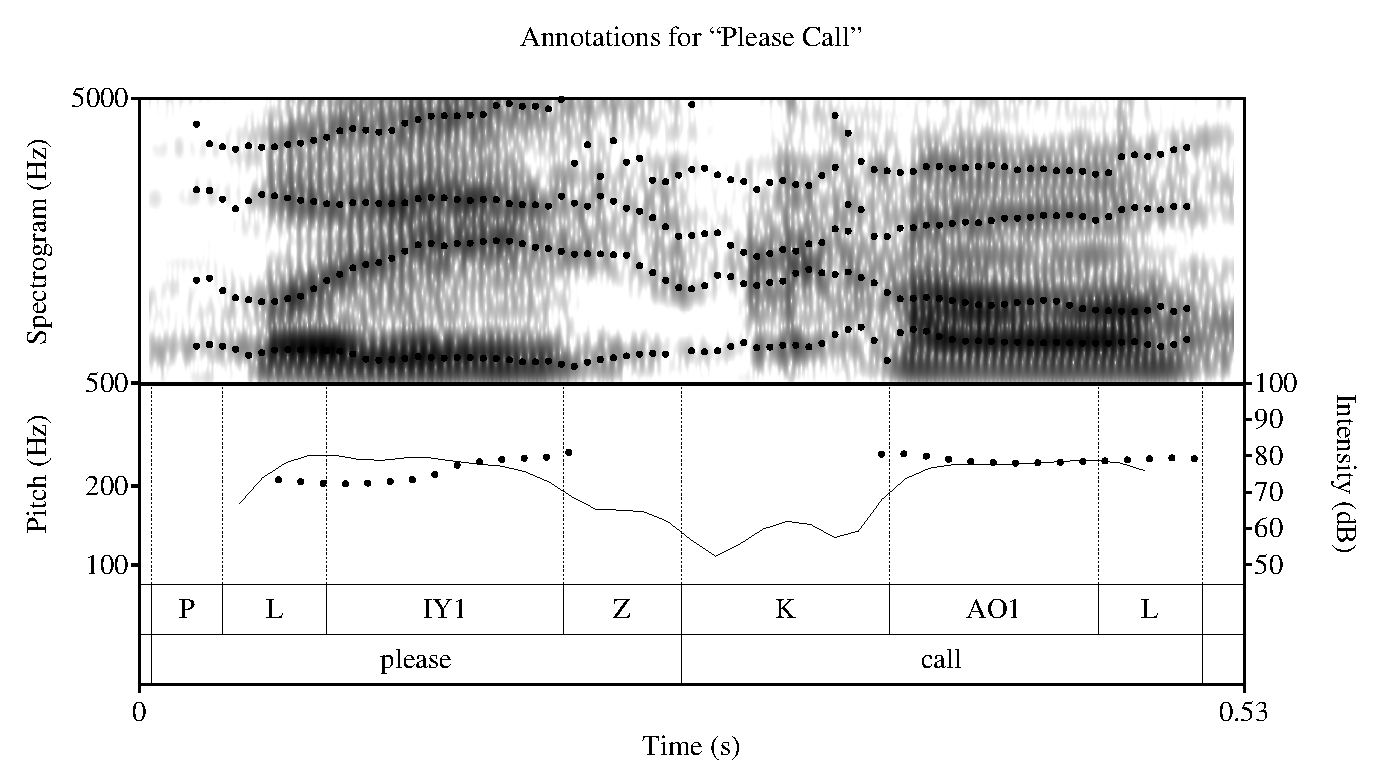
\includegraphics[width=0.8\textwidth]{figures/seg.eps}
    \caption{Illustration of Auto-segmentation}
    \label{fig:seg}
  \figSpace
\end{figure}

\subsection{Plosives}

Six L2 speech samples selected by the current study contained plosive-related mismatches as indicated by their respective IPA transcriptions. The following describes how the mismatches were verified by acoustic measurements. Duration of voice onset time (VOT) was used as the benchmark acoustic measurement for plosives. VOT duration of L2 segments and mean VOT duration of L1 segments were measured. 

VOT is defined as the interval between the onset of a plosive burst and the onset of the following vocalic onset. There are numerous claims that VOT directly affects accentedness perception \citep{Major_1987, Riney_1999}. Six L2 stimuli were therefore selected to verify these claims made in previous research. Following the practice of \citet{Chodroff_2017}, the beginning of the VOT was placed at the beginning of a plosive burst release; and the endpoint was placed at the beginning of periodicity in the waveform or a visible pitch track, whichever came first. VOT labeling was initially achieved in PRAAT with the AutoVOT plugin \citep{Keshet_2014}. Labeling errors were manually corrected in PRAAT based on waveforms and spectrograms. 

Contexts “\textit{please call},” “\textit{small plastic}” and “\textit{six spoons}” were used for the investigation of VOT-related consonant mismatches. Six L2 speech samples that were identified as having VOT-related mismatches were extracted for analysis. Two speech samples involved VOT-shortening on [kʰ] in the word “call,” one speech sample involves VOT-shortening on [pʰ] in the word “please,” one speech sample involves VOT-shortening on [pʰ] in the word “\textit{plastic},” two speech sample involve VOT-lengthening on [p] in the word “\textit{spoons}.” In addition to the L2 speech samples, VOTs of 50 L1 speech samples were measured for comparison. 

Table \ref{table:vot} illustrates the type of VOT-related consonant mismatches and the contexts where they occurred. Every row in Table \ref{table:vot} represents the VOT of a plosive segment. The mismatch column lists the type of VOT-related mismatches and the segments involved. The L2 VOT column contains durational measurements of the six L2 VOTs. L2 VOTs were converted to z-scores with regard to L1 English VOT means and standard deviations (SD). A z-score represents how many standard deviations an L2 VOT mean is from the mean L1 VOTs. A positive z-score means an L2 VOT is longer than the mean L1 VOT, while a negative z-score means an L2 VOT is shorter than the mean L1 VOT.

For example, the first row of Table \ref{table:vot} shows that an L2 stimulus “\textit{please call}” involves the de-aspiration of [kʰ] in the word “call.” The L2 segment [k] has a VOT of 33.01 milliseconds (ms). Calculation based on 50 L1 American English productions of “\textit{please call}” shows that the mean VOT of L1 [kʰ]s is 52.78 ms with a standard deviation of 13.71 ms. The z-score shows that the L2 VOT is 1.44 standard deviations below the L1 mean. 

\begin{table}[!h]
  \figSpace
  \centering
  \caption{L1 and L2 VOT Comparisons}
\label{table:vot}
    \begin{tabular}{llrrr}
    \toprule
   Contexts & Mismatches & L2 VOT (ms) & L1 (English) VOT (ms) & Z \\
    \midrule
    \textit{please call} & [kʰ]$\rightarrow$[k] & 33.01 & M=52.78; SD=13.71 & -1.44 \\
    \textit{please call} & [kʰ]$\rightarrow$[k] & 21.26 & M=52.78; SD=13.71 & -2.30 \\
    \textit{please call} & [pʰ]$\rightarrow$[p] & 10.05 & M=62.50; SD=18.06 & -2.91 \\
    \textit{small plastic} & [pʰ]$\rightarrow$[p] & 20.86 & M=62.84; SD=15.53 & -2.70 \\
    \textit{six spoons} & [p]$\rightarrow$[pʰ] & 45.33 & M=14.46; SD=7.15 & +4.32 \\
    \textit{six spoons} & [p]$\rightarrow$[pʰ] & 68.53 & M=14.46; SD=7.15 & +7.56 \\
    \bottomrule
    \end{tabular}%
  \figSpace
\end{table}%


As shown in Table 3.2, the shortened VOTs are indeed shorter than the L1 means, while the lengthened VOTs are indeed longer than the L1 means. Therefore, VOT differences between the L1 and L2 speech samples were successfully captured by the IPA transcriptions of the L2 speech sam- ples. These L2 speech samples were therefore chosen to represent VOT-related phonetic mismatches in L2 speech.

\subsection{Fricatives} 

Seven L2 stimuli were selected to investigate the perceptual accentedness of fricative-related mismatches. Four stimuli involve replacing L1 fricatives with other fricatives (e.g., [z]$\rightarrow$[s], [θ]$\rightarrow$[f]). Three stimuli involve replacing the interdental fricative /θ/ with /t/. The seven stimuli are listed in Table \ref{table:cog}. Analysis in this session concerns three types of benchmark acoustic signals, namely, Center of Gravity, pitch context, and noise ratio. These acoustic signals were selected to approximate differences in place and manner of articulation.

\subsubsection{Center of Gravity}

Previous research on the acoustic correlates of English fricatives has discovered that the Center of Gravity (COG) of fricatives is a reliable cue for place of articulation \citep{Jongman_2000}. COG is a measurement of energy concentration. Energy of a speech sound, as measured by amplitude, could be concentrated in either the higher frequencies or the lower frequencies of the sound. A smaller COG implies that the energy of a sound is concentrated in the lower frequencies. 

As a measurement for place of articulation, COG value decreases as place of articulation moves further back in the oral cavity. For example, alveolar fricatives (e.g., /s/ and /z/) have lower COGs than dental fricatives (e.g., /θ/ and /ð/), whose COGs are lower than labiodental fricatives (e.g., /f/ and /v/) (Jongman et al., 2000). Although COG is traditionally thought of as a cue for place of articulation, \citet{Jongman_2000} reported that COG is also a good indicator for voicing, with voiceless English fricatives having significantly higher COGs than their voiced counterparts. Table \ref{table:cog} lists the COGs of segments in the seven L2 and L1 stimuli selected by the current study.

% Table generated by Excel2LaTeX from sheet 'cog'
\begin{table}[h]
  \figSpace
  \centering
  \caption{L1 and L2 COG Comparisons}
\label{table:cog}
    \begin{tabular}{llrlr}
    \toprule
    Contexts & Mismatches & L2 COG (Semitone) & L1 COG (Semitone)&Z \\
    \midrule
    \textit{please call} & [z]$\rightarrow$[s] & 77.68 & M=71.14; SD=5.31 & +1.23 \\
    \textit{small plastic} & [s]$\rightarrow$[z] & 64.39 & M=71.30; SD=7.28 & -0.95 \\
    \textit{five thick} & [θ]$\rightarrow$[f] & 73.77 & M=64.37; SD=11.40 & +0.82 \\
    \textit{six spoons} & [z]$\rightarrow$[ʃ] & 71.10  & M=64.56; SD=8.86 & +0.73 \\
\textit{five thick}& [θ]$\rightarrow$[t̪] & 59.63 & M=64.37; SD=11.40 & -0.42 \\
\textit{five thick}& [θ]$\rightarrow$[t̪] & 63.27 & M=64.37; SD=11.40 & -0.10 \\
  \textit{five thick}& [θ]$\rightarrow$[t̪] & 42.63 & M=64.86; SD=9.71 & -2.29 \\
    \bottomrule
    \end{tabular}%
  \figSpace
\end{table}%

Every row of Table \ref{table:cog} shows the COGs of an L2 segment and the corresponding mean L1 COG value. For example, the first L2 stimulus is “\textit{please call}.” The coda of “\textit{please}” was transcribed as [s]. The L2 production therefore involves the devoicing of the [z] in “\textit{please}” (i.e., [z]$\rightarrow$[s]). The COG of the L2 segment [s] is 77.68 semitones, while its corresponding L1 segment [z] has a mean COG of 71.14 semitones with a standard deviation of 5.31. The L2 segment [s] is thus 1.23 standard deviations above the mean. This result is consistent with previous claims that COGs of voiceless fricatives are higher than COGs of their voiced counterparts. Therefore, the [s] was accepted by the current study as a correct transcription.

The second L2 stimulus “\textit{small plastic}” replaced the [s] in “\textit{small}” with a voiced [z]. The COG of this L2 segment [z] is lower than the mean COG of the corresponding L1 [s]s. This finding is also consistent with previous research, which showed that voiced fricatives have lower COGs than voiceless fricatives \citep{Jongman_2000}. Acoustic measurements for the third stimulus  show that the L2 segment [f] has a higher COG than its L1 target segment /θ/, which is consistent with previous findings that COG value increases as the place of articulation moves further front in the oral cavity \citep{Jongman_2000}. Given these results, the IPA transcriptions for the first three stimuli in Table \ref{table:cog} were considered accurate by the current study. The difference between the remaining four L2 stimuli and their corresponding L1 productions cannot be explained via the COG measurement. The following section discusses two additional acoustic measurements that could capture the difference between the remaining four L2 stimuli and their corresponding L1 productions.  

\subsubsection{Pitch Context}

The fourth L2 stimulus “\textit{six spoons}” changed the final consonant in “\textit{spoons}” from [z] to [ʃ]. The COG of the voiceless L2 segment [ʃ] is higher than the mean COG of its target L1 segment [z]. Previous research claimed that the COG of the post-alveolar fricative [ʃ] should be lower than both alveolar fricatives /s/ and /z/ \citep{Jongman_2000}. Based on the COG measurement, [ʃ] is perhaps not a correct transcription. However, acoustic correlates of English phonemes are multidimensional. COG values alone cannot explain why the final consonant of “\textit{spoons}” was transcribed as [ʃ]. 

In addition to COG values. the perception of /s/ and /ʃ/ could be affected by the pitch values of the preceding segments \citep{Niebuhr_2017}. Specifically, /s/ is more likely to be perceived as /ʃ/ when its preceding segment carries a higher pitch. In other words, the final consonant in “\textit{spoons}” could be an /s/, but was perceived and transcribed as [ʃ] because the penultimate segment /n/ carries a relatively higher pitch. To investigate whether the preceding pitch context of the final consonant in “\textit{spoons}” potentially affected transcribers’ perceptions, pitch values of the /n/s were extracted in PRAAT. Pitch values were extracted at the location of the energy peak in the amplitude spectrum, using methods described in \citet{De_Jong_2009}. Pitch values were converted to semitones relative to 100 Hertz to approximate the non-linear mapping between Hertz values and human perception. 

The L2 stimulus “\textit{six spoons}” was produced by a male Lamaholot speaker. The [n] of the L2 stimulus carries a pitch of 20.98 semitones. To calculate pitch values of the natively produced /n/s, productions of 25 male L1 American English speakers were similarly processed in PRAAT. Results showed L1 male speakers’ productions of the /n/ carry a mean pitch of 14.93 semitones, with the standard deviation of 3.27 semitones. The L2 /n/ thus indeed carries a relatively higher pitch than mean pitch values of the L1 /n/s. Therefore, there is a reason to believe that the pitch value of the penultimate consonant [n] in the L2 production of “\textit{spoons}” affected transcribers’ perception of the final consonant. This finding does not necessarily imply that the IPA transcriptions of the L2 stimulus are incorrect, but affirms the fact that acoustic correlates of phonemes are multidimensional. Therefore, the current study accepted the [ʃ] as a correct transcription.

\subsubsection{Noise Ratio}

In addition to the four stimuli analyzed above, there are three stimuli that involve the replacement of the dental fricative /θ/ with a dentalized [t̪]. As discussed above, COGs increase as the place of articulation moves farther front in the oral cavity. Therefore, dental [θ]s should have higher COGs than [t̪]s. Table \ref{table:cog} shows that the mean L1 COG of [θ]s is indeed higher than COGs of the [t̪]s. However, the difference between /θ/ and /t/ lies primarily on their respective manners of articulation, which is not captured by COG measurements. To inspect whether the [t̪]s are reliable transcriptions, the current study opted to use noise ratio to investigate the manner difference between fricative and plosive consonants.

Plosive consonants, such as the alveolar /t/, consist of a silent closure interval, which is followed by a frication noise burst and an interval of aspiration noise. Fricative consonants, such as /θ/, also consist of a silent closure interval, which is followed by a period of friction noise. The longer the closure interval, the more likely a fricative is perceived as an affricate \citep{Dorman_1980}. The shorter the duration of friction noise, the more likely a fricative is perceived as a plosive \citep{Dorman_1980}. 

To investigate durational measurements of the American English /θ/, the same 50 American English speakers’ productions of “\textit{five thick}” were used. Male and female samples were analyzed separately, because frication noise of females tends to be shorter than males \citep{Jongman_2000}. 

A possible confounding factor of durational measurements is speech rate. Intervals of closure and frication noise might be shortened in fast speech. In slow speech, the intervals could be lengthened. To control for speech rate, noise ratios were calculated. Noise ratios were defined as the ratio of fricative noise duration over the duration of the whole word \citep{Jongman_2000}. Word duration was defined as the interval between the onset of the frication to the end of the word. Closure intervals were not included in the total duration of a word, because the L1 and L2 segments are word initial. It is difficult to distinguish closure intervals of word-initial segments from speech pauses between words. Tabel \ref{table:nr} illustrates the noise ratios of the L1 and L2 segments.

% Table generated by Excel2LaTeX from sheet 'noise'
\begin{table}[!h]
  \figSpace
  \centering
  \caption{L1 and L2 Noise Ratio Comparisons}
\label{table:nr}
    \begin{tabular}{lllrr}
    \toprule
    Phrases & Gender & Mismatches & L2 Noise Ratio & L1 Noise Ratio \\
    \midrule
    \textit{five thick} & male  &  [θ]$\rightarrow$[t̪] & 0.17  & 0.25 \\
   \textit{five thick} & male  & [θ]$\rightarrow$[t̪] & 0.15  & 0.25 \\
   \textit{five thick} & female & [θ]$\rightarrow$[t̪] & 0.16  & 0.20 \\
    \bottomrule
    \end{tabular}%
  \figSpace
\end{table}%

The mean noise ratio for male L1 speakers is 0.25 (SD=0.06), and the mean noise ratio for female L1 speakers is 0.20 (SD=0.08). For the three L2 stimuli that replaced /θ/ with [t] or [t̪], noise durations were defined as the duration of the release burst and the aspiration noise. Word durations were defined as the interval from the onset of the release burst to the end of a word. As shown in Table \ref{table:nr}, the noise ratios for [t̪]s are 0.17, 0.15, and 0.16 respectively. In other words, L1 [θ]s, in general, have a longer frication noise duration than the noise durations (i.e. burst and aspiration noise) of the three corresponding L2 segments. Since shorter noise duration of a segment increases the chance for it to be perceived as a plosive consonant \citep{Jongman_1989}, there is reason to believe that the three L2 segments were transcribed correctly. These L2 stimuli were therefore accepted by the current study as representatives of /θ/-stopping (i.e., /θ/$\rightarrow$/t/). 

\subsection{Liquids}

In addition to plosives and fricatives, the current study also aims to investigate the accentedness of liquid productions in L2 speech. L2 speech involving the alternation between /ɹ/ and /l/ was often perceived by L1 American English listeners as very accented \citep{Riney_2005}. Eight L2 speech samples were selected to investigate the accentedness of syllable final /l/s and /ɹ/s. Based on findings in previous research, the degree of /l/-velarization was approximated by the difference between F1 and F2 \citep{Riney_2005} values. The degree of /ɹ/-rhoticity was approximated by the difference between F2 and the third formant frequencies (F3) \citep{Ohala_2001}. The F1, F2, and F2 values were extracted at the energy peak in the amplitude spectrum of the liquids.The following section discusses the analysis on L1 and L2 liquid productions in the phonological contexts of “\textit{small plastic}” and “\textit{ask her}.”

\subsubsection{Formant Information of L1 Liquids}

Previous acoustic research has shown that the velarization of the English word-final /l/ causes an increase in F1 and a decrease in F2, with respect to non-velarized /l/s \citep{Riney_2005}. Previous literature on world-final /ɹ/ often associates rhoticity with the lowering of F3. In addition to the English  /ɹ/s, low F3 for rhoticity was shown to hold for Malayalam rhotic trills, Toda trills, Tamil retroflex /ɭ/ and Hindi retroflex plosives \citep{Ohala_2001}. Indeed, the difference between F2 and F3 has been recommended as a reliable acoustic cue for automated measurement of rhotics \citep{Campbell_2018}. The current study therefore operationalized rhoticity by taking the difference between F2 and F3. 

The labeling of liquid segments was achieved via the Montreal Forced Aligner with manual adjustments afterwards. The beginning of a word-final liquid was set at the start of the F2 transition, while the end of a word-final liquid was set at the beginning of a pause between words or the following segment (whichever occurred first). F1, F2 and F3 values of each liquid were then extracted with PRAAT at the location of the energy peak in the amplitude spectrum, using methods described in \citep{De_Jong_2009}. Formant frequencies were then converted to semitones relative to 100 Hertz. 

Figure \ref{fig:l1_liquid} demonstrates the spectral information of word-final /l/s and /ɹ/s produced by the 50 native speakers of American English, where the bold phonetic symbols represent the means and the shaded areas represent one standard deviation around the means. The small gray symbols represent productions of the 50 native speakers of American English. Male and female productions were presented separately, because male voice frequencies are generally lower than female voice frequencies. In general, the /ɹ/s show a relatively smaller F3-F2 difference, demonstrating that the English word-final /ɹ/s are more rhotic than word-final /l/s. The word-final /l/s show a relatively small F2-F1 difference, demonstrating that the word-final /l/s have a higher degree of velarization than word-final /ɹ/s. 

\begin{figure}[h]
  \figSpace
    \centering
        \input{figures/chp3/liq1.tex}
	%\includegraphics[width=0.75\textwidth]{figures/liquids_native.png}
    \caption{Formant Information of L1 Liquids}
    \label{fig:l1_liquid}
  \figSpace
\end{figure}

\subsubsection{Formant Information of L2 Liquids}

Eight L2 speech samples were selected based on the vetted transcriptions, five of which involved the replacing of English word-final /ɹ/ with a trill /r/; the remaining three were /l/-related variations: two of the three replaced English word-final /l/ with a retroflexed /ɭ/, the third replaced /l/ with a flap /ɾ/. Labeling of L2 segments followed the same method as mentioned above. F1, F2, and F3 values were similarly extracted with PRAAT. Figure \ref{fig:l2_liquid} demonstrates the spectral information of both the L1 and L2 segments, while the phonetic symbols with a gray background represent L1 segments and the phonetic symbol without background represent the eight L2 segments. 

As Figure \ref{fig:l2_liquid} shows, both of the retroflexed [ɭ]s have a relatively smaller F3-F2 difference than English [l]s, showing that the [ɭ]s are likely to be more rhotic than their L1 counterparts. The L2 /r/s, on the other hand, have a relatively larger F3-F2 difference than the L1 /ɹ/s, showing that the L2 /r/s are less rhotic than their L1 counterparts. The eight L2 speech samples were therefore considered as correctly transcribed. They were consequently chosen to represent L2 liquid mismatches.

\begin{figure}[h]
  \figSpace
    \centering
            % Created by tikzDevice version 0.12.3 on 2019-11-29 00:11:10
% !TEX encoding = UTF-8 Unicode
\begin{tikzpicture}[x=1pt,y=1pt]
\definecolor{fillColor}{RGB}{255,255,255}
\path[use as bounding box,fill=fillColor,fill opacity=0.00] (0,0) rectangle (361.35,289.08);
\begin{scope}
\path[clip] (  0.00,  0.00) rectangle (361.35,289.08);
\definecolor{drawColor}{RGB}{255,255,255}
\definecolor{fillColor}{RGB}{255,255,255}

\path[draw=drawColor,line width= 0.6pt,line join=round,line cap=round,fill=fillColor] (  0.00,  0.00) rectangle (361.35,289.08);
\end{scope}
\begin{scope}
\path[clip] ( 31.71, 30.69) rectangle (191.03,267.01);
\definecolor{fillColor}{RGB}{255,255,255}

\path[fill=fillColor] ( 31.71, 30.69) rectangle (191.03,267.01);
\definecolor{drawColor}{gray}{0.92}

\path[draw=drawColor,line width= 0.3pt,line join=round] ( 31.71, 57.80) --
	(191.03, 57.80);

\path[draw=drawColor,line width= 0.3pt,line join=round] ( 31.71,108.00) --
	(191.03,108.00);

\path[draw=drawColor,line width= 0.3pt,line join=round] ( 31.71,158.20) --
	(191.03,158.20);

\path[draw=drawColor,line width= 0.3pt,line join=round] ( 31.71,208.39) --
	(191.03,208.39);

\path[draw=drawColor,line width= 0.3pt,line join=round] ( 31.71,258.59) --
	(191.03,258.59);

\path[draw=drawColor,line width= 0.3pt,line join=round] ( 52.12, 30.69) --
	( 52.12,267.01);

\path[draw=drawColor,line width= 0.3pt,line join=round] ( 93.62, 30.69) --
	( 93.62,267.01);

\path[draw=drawColor,line width= 0.3pt,line join=round] (135.11, 30.69) --
	(135.11,267.01);

\path[draw=drawColor,line width= 0.3pt,line join=round] (176.60, 30.69) --
	(176.60,267.01);

\path[draw=drawColor,line width= 0.6pt,line join=round] ( 31.71, 32.70) --
	(191.03, 32.70);

\path[draw=drawColor,line width= 0.6pt,line join=round] ( 31.71, 82.90) --
	(191.03, 82.90);

\path[draw=drawColor,line width= 0.6pt,line join=round] ( 31.71,133.10) --
	(191.03,133.10);

\path[draw=drawColor,line width= 0.6pt,line join=round] ( 31.71,183.30) --
	(191.03,183.30);

\path[draw=drawColor,line width= 0.6pt,line join=round] ( 31.71,233.49) --
	(191.03,233.49);

\path[draw=drawColor,line width= 0.6pt,line join=round] ( 72.87, 30.69) --
	( 72.87,267.01);

\path[draw=drawColor,line width= 0.6pt,line join=round] (114.36, 30.69) --
	(114.36,267.01);

\path[draw=drawColor,line width= 0.6pt,line join=round] (155.86, 30.69) --
	(155.86,267.01);
\definecolor{drawColor}{RGB}{190,190,190}

\node[text=drawColor,text opacity=0.80,anchor=base,inner sep=0pt, outer sep=0pt, scale=  1.14] at (173.47,155.07) {ɹ};

\node[text=drawColor,text opacity=0.80,anchor=base,inner sep=0pt, outer sep=0pt, scale=  1.14] at (181.98, 99.49) {ɹ};

\node[text=drawColor,text opacity=0.80,anchor=base,inner sep=0pt, outer sep=0pt, scale=  1.14] at (145.61,187.13) {ɹ};

\node[text=drawColor,text opacity=0.80,anchor=base,inner sep=0pt, outer sep=0pt, scale=  1.14] at (160.08,131.65) {ɹ};

\node[text=drawColor,text opacity=0.80,anchor=base,inner sep=0pt, outer sep=0pt, scale=  1.14] at (122.10,173.96) {ɹ};

\node[text=drawColor,text opacity=0.80,anchor=base,inner sep=0pt, outer sep=0pt, scale=  1.14] at (179.05,120.17) {ɹ};

\node[text=drawColor,text opacity=0.80,anchor=base,inner sep=0pt, outer sep=0pt, scale=  1.14] at (155.79,175.41) {ɹ};

\node[text=drawColor,text opacity=0.80,anchor=base,inner sep=0pt, outer sep=0pt, scale=  1.14] at (183.01,170.11) {ɹ};

\node[text=drawColor,text opacity=0.80,anchor=base,inner sep=0pt, outer sep=0pt, scale=  1.14] at (158.45, 62.95) {ɹ};

\node[text=drawColor,text opacity=0.80,anchor=base,inner sep=0pt, outer sep=0pt, scale=  1.14] at (159.07,129.23) {ɹ};

\node[text=drawColor,text opacity=0.80,anchor=base,inner sep=0pt, outer sep=0pt, scale=  1.14] at (162.33,128.61) {ɹ};

\node[text=drawColor,text opacity=0.80,anchor=base,inner sep=0pt, outer sep=0pt, scale=  1.14] at (156.64, 82.87) {ɹ};

\node[text=drawColor,text opacity=0.80,anchor=base,inner sep=0pt, outer sep=0pt, scale=  1.14] at (151.22,116.87) {ɹ};

\node[text=drawColor,text opacity=0.80,anchor=base,inner sep=0pt, outer sep=0pt, scale=  1.14] at (155.93,107.34) {ɹ};

\node[text=drawColor,text opacity=0.80,anchor=base,inner sep=0pt, outer sep=0pt, scale=  1.14] at (156.00,116.52) {ɹ};

\node[text=drawColor,text opacity=0.80,anchor=base,inner sep=0pt, outer sep=0pt, scale=  1.14] at (163.24, 80.75) {ɹ};

\node[text=drawColor,text opacity=0.80,anchor=base,inner sep=0pt, outer sep=0pt, scale=  1.14] at (164.70,139.50) {ɹ};

\node[text=drawColor,text opacity=0.80,anchor=base,inner sep=0pt, outer sep=0pt, scale=  1.14] at (162.53,105.34) {ɹ};

\node[text=drawColor,text opacity=0.80,anchor=base,inner sep=0pt, outer sep=0pt, scale=  1.14] at (171.49,174.14) {ɹ};

\node[text=drawColor,text opacity=0.80,anchor=base,inner sep=0pt, outer sep=0pt, scale=  1.14] at (169.28,196.18) {ɹ};

\node[text=drawColor,text opacity=0.80,anchor=base,inner sep=0pt, outer sep=0pt, scale=  1.14] at (161.48, 78.85) {ɹ};

\node[text=drawColor,text opacity=0.80,anchor=base,inner sep=0pt, outer sep=0pt, scale=  1.14] at (148.83,117.05) {ɹ};

\node[text=drawColor,text opacity=0.80,anchor=base,inner sep=0pt, outer sep=0pt, scale=  1.14] at (161.35,147.57) {ɹ};

\node[text=drawColor,text opacity=0.80,anchor=base,inner sep=0pt, outer sep=0pt, scale=  1.14] at (160.01, 88.93) {ɹ};

\node[text=drawColor,text opacity=0.80,anchor=base,inner sep=0pt, outer sep=0pt, scale=  1.14] at (162.13, 37.51) {ɹ};

\node[text=drawColor,text opacity=0.80,anchor=base,inner sep=0pt, outer sep=0pt, scale=  1.14] at (172.85,112.33) {ɹ};

\node[text=drawColor,text opacity=0.80,anchor=base,inner sep=0pt, outer sep=0pt, scale=  1.14] at (171.66,130.14) {ɹ};

\node[text=drawColor,text opacity=0.80,anchor=base,inner sep=0pt, outer sep=0pt, scale=  1.14] at (169.93, 72.60) {ɹ};

\node[text=drawColor,text opacity=0.80,anchor=base,inner sep=0pt, outer sep=0pt, scale=  1.14] at (133.66,135.45) {ɹ};

\node[text=drawColor,text opacity=0.80,anchor=base,inner sep=0pt, outer sep=0pt, scale=  1.14] at (181.08,186.81) {ɹ};

\node[text=drawColor,text opacity=0.80,anchor=base,inner sep=0pt, outer sep=0pt, scale=  1.14] at (177.43, 45.11) {ɹ};

\node[text=drawColor,text opacity=0.80,anchor=base,inner sep=0pt, outer sep=0pt, scale=  1.14] at (183.79,145.30) {ɹ};

\node[text=drawColor,text opacity=0.80,anchor=base,inner sep=0pt, outer sep=0pt, scale=  1.14] at (160.01, 41.39) {ɹ};

\node[text=drawColor,text opacity=0.80,anchor=base,inner sep=0pt, outer sep=0pt, scale=  1.14] at (152.51, 80.21) {ɹ};

\node[text=drawColor,text opacity=0.80,anchor=base,inner sep=0pt, outer sep=0pt, scale=  1.14] at (155.79,116.16) {ɹ};

\node[text=drawColor,text opacity=0.80,anchor=base,inner sep=0pt, outer sep=0pt, scale=  1.14] at (124.01,122.19) {ɹ};

\node[text=drawColor,text opacity=0.80,anchor=base,inner sep=0pt, outer sep=0pt, scale=  1.14] at (161.54,110.45) {ɹ};

\node[text=drawColor,text opacity=0.80,anchor=base,inner sep=0pt, outer sep=0pt, scale=  1.14] at (177.16,117.75) {ɹ};

\node[text=drawColor,text opacity=0.80,anchor=base,inner sep=0pt, outer sep=0pt, scale=  1.14] at (168.09,135.16) {ɹ};

\node[text=drawColor,text opacity=0.80,anchor=base,inner sep=0pt, outer sep=0pt, scale=  1.14] at (165.02,111.96) {ɹ};

\node[text=drawColor,text opacity=0.80,anchor=base,inner sep=0pt, outer sep=0pt, scale=  1.14] at (164.51, 88.69) {ɹ};

\node[text=drawColor,text opacity=0.80,anchor=base,inner sep=0pt, outer sep=0pt, scale=  1.14] at (164.38,111.96) {ɹ};

\node[text=drawColor,text opacity=0.80,anchor=base,inner sep=0pt, outer sep=0pt, scale=  1.14] at (157.55,182.43) {ɹ};

\node[text=drawColor,text opacity=0.80,anchor=base,inner sep=0pt, outer sep=0pt, scale=  1.14] at (172.46, 81.28) {ɹ};

\node[text=drawColor,text opacity=0.80,anchor=base,inner sep=0pt, outer sep=0pt, scale=  1.14] at (170.10, 81.02) {ɹ};

\node[text=drawColor,text opacity=0.80,anchor=base,inner sep=0pt, outer sep=0pt, scale=  1.14] at (168.80,176.40) {ɹ};

\node[text=drawColor,text opacity=0.80,anchor=base,inner sep=0pt, outer sep=0pt, scale=  1.14] at (178.11,187.68) {ɹ};

\node[text=drawColor,text opacity=0.80,anchor=base,inner sep=0pt, outer sep=0pt, scale=  1.14] at (162.79, 66.81) {ɹ};

\node[text=drawColor,text opacity=0.80,anchor=base,inner sep=0pt, outer sep=0pt, scale=  1.14] at (133.37,215.53) {l};

\node[text=drawColor,text opacity=0.80,anchor=base,inner sep=0pt, outer sep=0pt, scale=  1.14] at (148.28,216.83) {l};

\node[text=drawColor,text opacity=0.80,anchor=base,inner sep=0pt, outer sep=0pt, scale=  1.14] at (123.68,237.04) {l};

\node[text=drawColor,text opacity=0.80,anchor=base,inner sep=0pt, outer sep=0pt, scale=  1.14] at ( 88.20,233.73) {l};

\node[text=drawColor,text opacity=0.80,anchor=base,inner sep=0pt, outer sep=0pt, scale=  1.14] at (170.97,198.08) {l};

\node[text=drawColor,text opacity=0.80,anchor=base,inner sep=0pt, outer sep=0pt, scale=  1.14] at (154.57,229.58) {l};

\node[text=drawColor,text opacity=0.80,anchor=base,inner sep=0pt, outer sep=0pt, scale=  1.14] at (111.03,235.02) {l};

\node[text=drawColor,text opacity=0.80,anchor=base,inner sep=0pt, outer sep=0pt, scale=  1.14] at (125.22,235.24) {l};

\node[text=drawColor,text opacity=0.80,anchor=base,inner sep=0pt, outer sep=0pt, scale=  1.14] at ( 78.42,225.01) {l};

\node[text=drawColor,text opacity=0.80,anchor=base,inner sep=0pt, outer sep=0pt, scale=  1.14] at ( 75.65,238.71) {l};

\node[text=drawColor,text opacity=0.80,anchor=base,inner sep=0pt, outer sep=0pt, scale=  1.14] at ( 44.20,230.92) {l};

\node[text=drawColor,text opacity=0.80,anchor=base,inner sep=0pt, outer sep=0pt, scale=  1.14] at ( 79.05,242.92) {l};

\node[text=drawColor,text opacity=0.80,anchor=base,inner sep=0pt, outer sep=0pt, scale=  1.14] at ( 45.54,247.80) {l};

\node[text=drawColor,text opacity=0.80,anchor=base,inner sep=0pt, outer sep=0pt, scale=  1.14] at ( 95.33,207.56) {l};

\node[text=drawColor,text opacity=0.80,anchor=base,inner sep=0pt, outer sep=0pt, scale=  1.14] at ( 78.00,224.08) {l};

\node[text=drawColor,text opacity=0.80,anchor=base,inner sep=0pt, outer sep=0pt, scale=  1.14] at ( 94.33,223.26) {l};

\node[text=drawColor,text opacity=0.80,anchor=base,inner sep=0pt, outer sep=0pt, scale=  1.14] at (109.68,229.92) {l};

\node[text=drawColor,text opacity=0.80,anchor=base,inner sep=0pt, outer sep=0pt, scale=  1.14] at ( 89.47,204.64) {l};

\node[text=drawColor,text opacity=0.80,anchor=base,inner sep=0pt, outer sep=0pt, scale=  1.14] at (127.27,224.75) {l};

\node[text=drawColor,text opacity=0.80,anchor=base,inner sep=0pt, outer sep=0pt, scale=  1.14] at (151.15,244.11) {l};

\node[text=drawColor,text opacity=0.80,anchor=base,inner sep=0pt, outer sep=0pt, scale=  1.14] at ( 76.51,242.83) {l};

\node[text=drawColor,text opacity=0.80,anchor=base,inner sep=0pt, outer sep=0pt, scale=  1.14] at (117.51,222.58) {l};

\node[text=drawColor,text opacity=0.80,anchor=base,inner sep=0pt, outer sep=0pt, scale=  1.14] at ( 86.72,220.08) {l};

\node[text=drawColor,text opacity=0.80,anchor=base,inner sep=0pt, outer sep=0pt, scale=  1.14] at ( 64.36,212.99) {l};

\node[text=drawColor,text opacity=0.80,anchor=base,inner sep=0pt, outer sep=0pt, scale=  1.14] at (103.60,224.70) {l};

\node[text=drawColor,text opacity=0.80,anchor=base,inner sep=0pt, outer sep=0pt, scale=  1.14] at ( 94.16,223.77) {l};

\node[text=drawColor,text opacity=0.80,anchor=base,inner sep=0pt, outer sep=0pt, scale=  1.14] at ( 60.70,231.92) {l};

\node[text=drawColor,text opacity=0.80,anchor=base,inner sep=0pt, outer sep=0pt, scale=  1.14] at (158.93,212.47) {l};

\node[text=drawColor,text opacity=0.80,anchor=base,inner sep=0pt, outer sep=0pt, scale=  1.14] at (135.10,220.72) {l};

\node[text=drawColor,text opacity=0.80,anchor=base,inner sep=0pt, outer sep=0pt, scale=  1.14] at (142.51,191.74) {l};

\node[text=drawColor,text opacity=0.80,anchor=base,inner sep=0pt, outer sep=0pt, scale=  1.14] at ( 96.48,237.17) {l};

\node[text=drawColor,text opacity=0.80,anchor=base,inner sep=0pt, outer sep=0pt, scale=  1.14] at (104.19,235.38) {l};

\node[text=drawColor,text opacity=0.80,anchor=base,inner sep=0pt, outer sep=0pt, scale=  1.14] at ( 99.82,231.96) {l};

\node[text=drawColor,text opacity=0.80,anchor=base,inner sep=0pt, outer sep=0pt, scale=  1.14] at ( 70.69,245.98) {l};

\node[text=drawColor,text opacity=0.80,anchor=base,inner sep=0pt, outer sep=0pt, scale=  1.14] at ( 38.95,252.35) {l};

\node[text=drawColor,text opacity=0.80,anchor=base,inner sep=0pt, outer sep=0pt, scale=  1.14] at (106.78,209.41) {l};

\node[text=drawColor,text opacity=0.80,anchor=base,inner sep=0pt, outer sep=0pt, scale=  1.14] at (153.10,215.87) {l};

\node[text=drawColor,text opacity=0.80,anchor=base,inner sep=0pt, outer sep=0pt, scale=  1.14] at ( 64.61,232.48) {l};

\node[text=drawColor,text opacity=0.80,anchor=base,inner sep=0pt, outer sep=0pt, scale=  1.14] at (137.81,239.88) {l};

\node[text=drawColor,text opacity=0.80,anchor=base,inner sep=0pt, outer sep=0pt, scale=  1.14] at (114.15,223.26) {l};

\node[text=drawColor,text opacity=0.80,anchor=base,inner sep=0pt, outer sep=0pt, scale=  1.14] at (115.16,232.29) {l};

\node[text=drawColor,text opacity=0.80,anchor=base,inner sep=0pt, outer sep=0pt, scale=  1.14] at ( 87.46,233.78) {l};

\node[text=drawColor,text opacity=0.80,anchor=base,inner sep=0pt, outer sep=0pt, scale=  1.14] at (128.84,208.05) {l};

\node[text=drawColor,text opacity=0.80,anchor=base,inner sep=0pt, outer sep=0pt, scale=  1.14] at (137.07,219.10) {l};

\node[text=drawColor,text opacity=0.80,anchor=base,inner sep=0pt, outer sep=0pt, scale=  1.14] at (133.56,238.75) {l};

\node[text=drawColor,text opacity=0.80,anchor=base,inner sep=0pt, outer sep=0pt, scale=  1.14] at (121.30,230.16) {l};

\node[text=drawColor,text opacity=0.80,anchor=base,inner sep=0pt, outer sep=0pt, scale=  1.14] at ( 85.02,194.53) {l};
\definecolor{drawColor}{RGB}{0,0,0}
\definecolor{fillColor}{RGB}{190,190,190}

\path[draw=drawColor,line width= 0.3pt,line join=round,line cap=round,fill=fillColor] (105.21,221.86) --
	(112.36,221.86) --
	(112.29,221.86) --
	(112.58,221.88) --
	(112.86,221.93) --
	(113.13,222.04) --
	(113.38,222.18) --
	(113.61,222.37) --
	(113.80,222.58) --
	(113.96,222.83) --
	(114.07,223.10) --
	(114.14,223.38) --
	(114.17,223.67) --
	(114.17,223.67) --
	(114.17,237.84) --
	(114.17,237.84) --
	(114.14,238.12) --
	(114.07,238.41) --
	(113.96,238.67) --
	(113.80,238.92) --
	(113.61,239.14) --
	(113.38,239.32) --
	(113.13,239.47) --
	(112.86,239.57) --
	(112.58,239.63) --
	(112.36,239.64) --
	(105.21,239.64) --
	(105.43,239.63) --
	(105.14,239.64) --
	(104.85,239.61) --
	(104.57,239.52) --
	(104.31,239.40) --
	(104.07,239.23) --
	(103.86,239.03) --
	(103.68,238.80) --
	(103.55,238.54) --
	(103.45,238.27) --
	(103.41,237.98) --
	(103.40,237.84) --
	(103.40,223.67) --
	(103.41,223.81) --
	(103.41,223.52) --
	(103.45,223.24) --
	(103.55,222.96) --
	(103.68,222.70) --
	(103.86,222.47) --
	(104.07,222.27) --
	(104.31,222.10) --
	(104.57,221.98) --
	(104.85,221.90) --
	(105.14,221.86) --
	cycle;
\end{scope}
\begin{scope}
\path[clip] ( 31.71, 30.69) rectangle (191.03,267.01);
\definecolor{drawColor}{RGB}{0,0,0}

\node[text=drawColor,anchor=base,inner sep=0pt, outer sep=0pt, scale=  1.5] at (108.78,224.87) {l};
\definecolor{fillColor}{RGB}{190,190,190}

\path[draw=drawColor,line width= 0.3pt,line join=round,line cap=round,fill=fillColor] (159.31,110.62) --
	(168.40,110.62) --
	(168.33,110.62) --
	(168.62,110.64) --
	(168.91,110.69) --
	(169.18,110.80) --
	(169.43,110.94) --
	(169.65,111.13) --
	(169.85,111.34) --
	(170.00,111.59) --
	(170.12,111.86) --
	(170.19,112.14) --
	(170.21,112.43) --
	(170.21,112.43) --
	(170.21,126.59) --
	(170.21,126.59) --
	(170.19,126.88) --
	(170.12,127.17) --
	(170.00,127.43) --
	(169.85,127.68) --
	(169.65,127.90) --
	(169.43,128.08) --
	(169.18,128.23) --
	(168.91,128.33) --
	(168.62,128.39) --
	(168.40,128.40) --
	(159.31,128.40) --
	(159.53,128.39) --
	(159.24,128.40) --
	(158.95,128.37) --
	(158.67,128.28) --
	(158.41,128.16) --
	(158.17,127.99) --
	(157.96,127.79) --
	(157.78,127.56) --
	(157.65,127.30) --
	(157.56,127.03) --
	(157.51,126.74) --
	(157.50,126.59) --
	(157.50,112.43) --
	(157.51,112.57) --
	(157.51,112.28) --
	(157.56,112.00) --
	(157.65,111.72) --
	(157.78,111.46) --
	(157.96,111.23) --
	(158.17,111.03) --
	(158.41,110.86) --
	(158.67,110.74) --
	(158.95,110.66) --
	(159.24,110.62) --
	cycle;
\end{scope}
\begin{scope}
\path[clip] ( 31.71, 30.69) rectangle (191.03,267.01);
\definecolor{drawColor}{RGB}{0,0,0}

\node[text=drawColor,anchor=base,inner sep=0pt, outer sep=0pt, scale=  1.5] at (163.86,113.63) {ɹ};
\definecolor{fillColor}{RGB}{255,255,255}

%\path[draw=drawColor,line width= 0.0pt,line join=round,line cap=round,fill=fillColor] (161.05,174.84) --
	(179.62,174.84) --
	(179.55,174.84) --
	(179.84,174.85) --
	(180.12,174.91) --
	(180.40,175.02) --
	(180.65,175.16) --
	(180.87,175.34) --
	(181.07,175.56) --
	(181.22,175.81) --
	(181.33,176.08) --
	(181.40,176.36) --
	(181.43,176.65) --
	(181.43,176.65) --
	(181.43,190.81) --
	(181.43,190.81) --
	(181.40,191.10) --
	(181.33,191.39) --
	(181.22,191.65) --
	(181.07,191.90) --
	(180.87,192.12) --
	(180.65,192.30) --
	(180.40,192.45) --
	(180.12,192.55) --
	(179.84,192.61) --
	(179.62,192.62) --
	(161.05,192.62) --
	(161.26,192.61) --
	(160.97,192.62) --
	(160.69,192.58) --
	(160.41,192.50) --
	(160.14,192.38) --
	(159.90,192.21) --
	(159.69,192.01) --
	(159.52,191.78) --
	(159.38,191.52) --
	(159.29,191.25) --
	(159.25,190.96) --
	(159.24,190.81) --
	(159.24,176.65) --
	(159.25,176.79) --
	(159.25,176.50) --
	(159.29,176.22) --
	(159.38,175.94) --
	(159.52,175.68) --
	(159.69,175.45) --
	(159.90,175.25) --
	(160.14,175.08) --
	(160.41,174.96) --
	(160.69,174.88) --
	(160.97,174.84) --
	cycle;
\end{scope}
\begin{scope}
\path[clip] ( 31.71, 30.69) rectangle (191.03,267.01);
\definecolor{drawColor}{RGB}{0,0,0}

\node[text=drawColor,anchor=base,inner sep=0pt, outer sep=0pt, scale=  1.5] at (170.33,177.85) {r};

%\path[draw=drawColor,line width= 0.0pt,line join=round,line cap=round] (167.41,190.50) --
	(179.30,190.50) --
	(179.23,190.50) --
	(179.52,190.51) --
	(179.80,190.57) --
	(180.08,190.67) --
	(180.33,190.82) --
	(180.55,191.00) --
	(180.75,191.22) --
	(180.90,191.47) --
	(181.02,191.73) --
	(181.09,192.02) --
	(181.11,192.31) --
	(181.11,192.31) --
	(181.11,206.47) --
	(181.11,206.47) --
	(181.09,206.76) --
	(181.02,207.04) --
	(180.90,207.31) --
	(180.75,207.56) --
	(180.55,207.77) --
	(180.33,207.96) --
	(180.08,208.10) --
	(179.80,208.21) --
	(179.52,208.27) --
	(179.30,208.28) --
	(167.41,208.28) --
	(167.63,208.27) --
	(167.34,208.28) --
	(167.05,208.24) --
	(166.77,208.16) --
	(166.51,208.04) --
	(166.27,207.87) --
	(166.06,207.67) --
	(165.89,207.44) --
	(165.75,207.18) --
	(165.66,206.90) --
	(165.61,206.62) --
	(165.61,206.47) --
	(165.61,192.31) --
	(165.61,192.45) --
	(165.61,192.16) --
	(165.66,191.87) --
	(165.75,191.60) --
	(165.89,191.34) --
	(166.06,191.11) --
	(166.27,190.91) --
	(166.51,190.74) --
	(166.77,190.62) --
	(167.05,190.54) --
	(167.34,190.50) --
	(167.41,190.50);
\end{scope}
\begin{scope}
\path[clip] ( 31.71, 30.69) rectangle (191.03,267.01);
\definecolor{drawColor}{RGB}{0,0,0}

\node[text=drawColor,anchor=base,inner sep=0pt, outer sep=0pt, scale=  1.5] at (173.36,193.51) {ɭ};

%\path[draw=drawColor,line width= 0.0pt,line join=round,line cap=round] (170.68,181.84) --
	(189.26,181.84) --
	(189.18,181.84) --
	(189.47,181.86) --
	(189.76,181.91) --
	(190.03,182.02) --
	(190.28,182.16) --
	(190.51,182.35) --
	(190.70,182.56) --
	(190.86,182.81) --
	(190.97,183.08) --
	(191.04,183.36) --
	(191.06,183.65) --
	(191.06,183.65) --
	(191.06,197.82) --
	(191.06,197.82) --
	(191.04,198.11) --
	(190.97,198.39) --
	(190.86,198.66) --
	(190.70,198.90) --
	(190.51,199.12) --
	(190.28,199.30) --
	(190.03,199.45) --
	(189.76,199.55) --
	(189.47,199.61) --
	(189.26,199.62) --
	(170.68,199.62) --
	(170.90,199.61) --
	(170.61,199.62) --
	(170.32,199.59) --
	(170.04,199.50) --
	(169.78,199.38) --
	(169.54,199.21) --
	(169.33,199.01) --
	(169.16,198.78) --
	(169.02,198.52) --
	(168.93,198.25) --
	(168.88,197.96) --
	(168.88,197.82) --
	(168.88,183.65) --
	(168.88,183.80) --
	(168.88,183.50) --
	(168.93,183.22) --
	(169.02,182.94) --
	(169.16,182.68) --
	(169.33,182.45) --
	(169.54,182.25) --
	(169.78,182.09) --
	(170.04,181.96) --
	(170.32,181.88) --
	(170.61,181.84) --
	(170.68,181.84);
\end{scope}
\begin{scope}
\path[clip] ( 31.71, 30.69) rectangle (191.03,267.01);
\definecolor{drawColor}{RGB}{0,0,0}

\node[text=drawColor,anchor=base,inner sep=0pt, outer sep=0pt, scale=  1.5] at (179.97,184.85) {r};
\definecolor{drawColor}{RGB}{190,190,190}
\definecolor{fillColor}{RGB}{255,255,255}

\path[draw=drawColor,line width= 0.6pt,line join=round,line cap=round,fill=fillColor,fill opacity=0.10] (148.74,224.18) --
	(148.41,226.23) --
	(147.43,228.35) --
	(145.81,230.52) --
	(143.59,232.69) --
	(140.79,234.83) --
	(137.45,236.92) --
	(133.62,238.92) --
	(129.37,240.80) --
	(124.76,242.54) --
	(119.86,244.10) --
	(114.74,245.46) --
	(109.47,246.60) --
	(104.15,247.51) --
	( 98.85,248.17) --
	( 93.65,248.57) --
	( 88.62,248.70) --
	( 83.86,248.56) --
	( 79.42,248.16) --
	( 75.37,247.51) --
	( 71.78,246.60) --
	( 68.71,245.45) --
	( 66.19,244.09) --
	( 64.26,242.53) --
	( 62.97,240.80) --
	( 62.31,238.91) --
	( 62.31,236.91) --
	( 62.97,234.82) --
	( 64.26,232.68) --
	( 66.19,230.50) --
	( 68.71,228.34) --
	( 71.78,226.22) --
	( 75.37,224.17) --
	( 79.42,222.23) --
	( 83.86,220.41) --
	( 88.62,218.77) --
	( 93.65,217.30) --
	( 98.85,216.05) --
	(104.15,215.02) --
	(109.47,214.24) --
	(114.74,213.71) --
	(119.86,213.44) --
	(124.76,213.44) --
	(129.37,213.71) --
	(133.62,214.24) --
	(137.45,215.03) --
	(140.79,216.05) --
	(143.59,217.31) --
	(145.81,218.77) --
	(147.43,220.42) --
	(148.41,222.24) --
	(148.74,224.18) --
	cycle;

\path[draw=drawColor,line width= 0.6pt,line join=round,line cap=round,fill=fillColor,fill opacity=0.10] (179.02,125.33) --
	(178.91,132.09) --
	(178.56,138.67) --
	(178.00,144.98) --
	(177.22,150.93) --
	(176.23,156.41) --
	(175.06,161.36) --
	(173.72,165.68) --
	(172.22,169.33) --
	(170.61,172.24) --
	(168.88,174.37) --
	(167.08,175.68) --
	(165.24,176.16) --
	(163.37,175.80) --
	(161.51,174.61) --
	(159.68,172.59) --
	(157.92,169.79) --
	(156.24,166.25) --
	(154.68,162.02) --
	(153.26,157.16) --
	(152.00,151.74) --
	(150.92,145.86) --
	(150.04,139.59) --
	(149.36,133.04) --
	(148.91,126.30) --
	(148.68,119.48) --
	(148.68,112.68) --
	(148.91,105.99) --
	(149.36, 99.53) --
	(150.04, 93.39) --
	(150.92, 87.67) --
	(152.00, 82.44) --
	(153.26, 77.80) --
	(154.68, 73.80) --
	(156.24, 70.52) --
	(157.92, 68.00) --
	(159.68, 66.27) --
	(161.51, 65.37) --
	(163.37, 65.31) --
	(165.24, 66.09) --
	(167.08, 67.70) --
	(168.88, 70.11) --
	(170.61, 73.29) --
	(172.22, 77.18) --
	(173.72, 81.74) --
	(175.06, 86.88) --
	(176.23, 92.54) --
	(177.22, 98.63) --
	(178.00,105.05) --
	(178.56,111.71) --
	(178.91,118.50) --
	(179.02,125.33) --
	cycle;
\definecolor{drawColor}{gray}{0.20}

\path[draw=drawColor,line width= 0.6pt,line join=round,line cap=round] ( 31.71, 30.69) rectangle (191.03,267.01);
\end{scope}
\begin{scope}
\path[clip] (196.53, 30.69) rectangle (355.85,267.01);
\definecolor{fillColor}{RGB}{255,255,255}

\path[fill=fillColor] (196.53, 30.69) rectangle (355.85,267.01);
\definecolor{drawColor}{gray}{0.92}

\path[draw=drawColor,line width= 0.3pt,line join=round] (196.53, 57.80) --
	(355.85, 57.80);

\path[draw=drawColor,line width= 0.3pt,line join=round] (196.53,108.00) --
	(355.85,108.00);

\path[draw=drawColor,line width= 0.3pt,line join=round] (196.53,158.20) --
	(355.85,158.20);

\path[draw=drawColor,line width= 0.3pt,line join=round] (196.53,208.39) --
	(355.85,208.39);

\path[draw=drawColor,line width= 0.3pt,line join=round] (196.53,258.59) --
	(355.85,258.59);

\path[draw=drawColor,line width= 0.3pt,line join=round] (216.94, 30.69) --
	(216.94,267.01);

\path[draw=drawColor,line width= 0.3pt,line join=round] (258.44, 30.69) --
	(258.44,267.01);

\path[draw=drawColor,line width= 0.3pt,line join=round] (299.93, 30.69) --
	(299.93,267.01);

\path[draw=drawColor,line width= 0.3pt,line join=round] (341.42, 30.69) --
	(341.42,267.01);

\path[draw=drawColor,line width= 0.6pt,line join=round] (196.53, 32.70) --
	(355.85, 32.70);

\path[draw=drawColor,line width= 0.6pt,line join=round] (196.53, 82.90) --
	(355.85, 82.90);

\path[draw=drawColor,line width= 0.6pt,line join=round] (196.53,133.10) --
	(355.85,133.10);

\path[draw=drawColor,line width= 0.6pt,line join=round] (196.53,183.30) --
	(355.85,183.30);

\path[draw=drawColor,line width= 0.6pt,line join=round] (196.53,233.49) --
	(355.85,233.49);

\path[draw=drawColor,line width= 0.6pt,line join=round] (237.69, 30.69) --
	(237.69,267.01);

\path[draw=drawColor,line width= 0.6pt,line join=round] (279.18, 30.69) --
	(279.18,267.01);

\path[draw=drawColor,line width= 0.6pt,line join=round] (320.68, 30.69) --
	(320.68,267.01);
\definecolor{drawColor}{RGB}{190,190,190}

\node[text=drawColor,text opacity=0.80,anchor=base,inner sep=0pt, outer sep=0pt, scale=  1.14] at (338.29,155.07) {ɹ};

\node[text=drawColor,text opacity=0.80,anchor=base,inner sep=0pt, outer sep=0pt, scale=  1.14] at (346.80, 99.49) {ɹ};

\node[text=drawColor,text opacity=0.80,anchor=base,inner sep=0pt, outer sep=0pt, scale=  1.14] at (310.43,187.13) {ɹ};

\node[text=drawColor,text opacity=0.80,anchor=base,inner sep=0pt, outer sep=0pt, scale=  1.14] at (324.90,131.65) {ɹ};

\node[text=drawColor,text opacity=0.80,anchor=base,inner sep=0pt, outer sep=0pt, scale=  1.14] at (286.92,173.96) {ɹ};

\node[text=drawColor,text opacity=0.80,anchor=base,inner sep=0pt, outer sep=0pt, scale=  1.14] at (343.87,120.17) {ɹ};

\node[text=drawColor,text opacity=0.80,anchor=base,inner sep=0pt, outer sep=0pt, scale=  1.14] at (320.61,175.41) {ɹ};

\node[text=drawColor,text opacity=0.80,anchor=base,inner sep=0pt, outer sep=0pt, scale=  1.14] at (347.83,170.11) {ɹ};

\node[text=drawColor,text opacity=0.80,anchor=base,inner sep=0pt, outer sep=0pt, scale=  1.14] at (323.27, 62.95) {ɹ};

\node[text=drawColor,text opacity=0.80,anchor=base,inner sep=0pt, outer sep=0pt, scale=  1.14] at (323.89,129.23) {ɹ};

\node[text=drawColor,text opacity=0.80,anchor=base,inner sep=0pt, outer sep=0pt, scale=  1.14] at (327.15,128.61) {ɹ};

\node[text=drawColor,text opacity=0.80,anchor=base,inner sep=0pt, outer sep=0pt, scale=  1.14] at (321.46, 82.87) {ɹ};

\node[text=drawColor,text opacity=0.80,anchor=base,inner sep=0pt, outer sep=0pt, scale=  1.14] at (316.04,116.87) {ɹ};

\node[text=drawColor,text opacity=0.80,anchor=base,inner sep=0pt, outer sep=0pt, scale=  1.14] at (320.75,107.34) {ɹ};

\node[text=drawColor,text opacity=0.80,anchor=base,inner sep=0pt, outer sep=0pt, scale=  1.14] at (320.82,116.52) {ɹ};

\node[text=drawColor,text opacity=0.80,anchor=base,inner sep=0pt, outer sep=0pt, scale=  1.14] at (328.06, 80.75) {ɹ};

\node[text=drawColor,text opacity=0.80,anchor=base,inner sep=0pt, outer sep=0pt, scale=  1.14] at (329.52,139.50) {ɹ};

\node[text=drawColor,text opacity=0.80,anchor=base,inner sep=0pt, outer sep=0pt, scale=  1.14] at (327.34,105.34) {ɹ};

\node[text=drawColor,text opacity=0.80,anchor=base,inner sep=0pt, outer sep=0pt, scale=  1.14] at (336.31,174.14) {ɹ};

\node[text=drawColor,text opacity=0.80,anchor=base,inner sep=0pt, outer sep=0pt, scale=  1.14] at (334.10,196.18) {ɹ};

\node[text=drawColor,text opacity=0.80,anchor=base,inner sep=0pt, outer sep=0pt, scale=  1.14] at (326.30, 78.85) {ɹ};

\node[text=drawColor,text opacity=0.80,anchor=base,inner sep=0pt, outer sep=0pt, scale=  1.14] at (313.65,117.05) {ɹ};

\node[text=drawColor,text opacity=0.80,anchor=base,inner sep=0pt, outer sep=0pt, scale=  1.14] at (326.17,147.57) {ɹ};

\node[text=drawColor,text opacity=0.80,anchor=base,inner sep=0pt, outer sep=0pt, scale=  1.14] at (324.83, 88.93) {ɹ};

\node[text=drawColor,text opacity=0.80,anchor=base,inner sep=0pt, outer sep=0pt, scale=  1.14] at (326.95, 37.51) {ɹ};

\node[text=drawColor,text opacity=0.80,anchor=base,inner sep=0pt, outer sep=0pt, scale=  1.14] at (337.67,112.33) {ɹ};

\node[text=drawColor,text opacity=0.80,anchor=base,inner sep=0pt, outer sep=0pt, scale=  1.14] at (336.48,130.14) {ɹ};

\node[text=drawColor,text opacity=0.80,anchor=base,inner sep=0pt, outer sep=0pt, scale=  1.14] at (334.74, 72.60) {ɹ};

\node[text=drawColor,text opacity=0.80,anchor=base,inner sep=0pt, outer sep=0pt, scale=  1.14] at (298.48,135.45) {ɹ};

\node[text=drawColor,text opacity=0.80,anchor=base,inner sep=0pt, outer sep=0pt, scale=  1.14] at (345.90,186.81) {ɹ};

\node[text=drawColor,text opacity=0.80,anchor=base,inner sep=0pt, outer sep=0pt, scale=  1.14] at (342.25, 45.11) {ɹ};

\node[text=drawColor,text opacity=0.80,anchor=base,inner sep=0pt, outer sep=0pt, scale=  1.14] at (348.61,145.30) {ɹ};

\node[text=drawColor,text opacity=0.80,anchor=base,inner sep=0pt, outer sep=0pt, scale=  1.14] at (324.83, 41.39) {ɹ};

\node[text=drawColor,text opacity=0.80,anchor=base,inner sep=0pt, outer sep=0pt, scale=  1.14] at (317.32, 80.21) {ɹ};

\node[text=drawColor,text opacity=0.80,anchor=base,inner sep=0pt, outer sep=0pt, scale=  1.14] at (320.61,116.16) {ɹ};

\node[text=drawColor,text opacity=0.80,anchor=base,inner sep=0pt, outer sep=0pt, scale=  1.14] at (288.83,122.19) {ɹ};

\node[text=drawColor,text opacity=0.80,anchor=base,inner sep=0pt, outer sep=0pt, scale=  1.14] at (326.36,110.45) {ɹ};

\node[text=drawColor,text opacity=0.80,anchor=base,inner sep=0pt, outer sep=0pt, scale=  1.14] at (341.98,117.75) {ɹ};

\node[text=drawColor,text opacity=0.80,anchor=base,inner sep=0pt, outer sep=0pt, scale=  1.14] at (332.90,135.16) {ɹ};

\node[text=drawColor,text opacity=0.80,anchor=base,inner sep=0pt, outer sep=0pt, scale=  1.14] at (329.83,111.96) {ɹ};

\node[text=drawColor,text opacity=0.80,anchor=base,inner sep=0pt, outer sep=0pt, scale=  1.14] at (329.33, 88.69) {ɹ};

\node[text=drawColor,text opacity=0.80,anchor=base,inner sep=0pt, outer sep=0pt, scale=  1.14] at (329.20,111.96) {ɹ};

\node[text=drawColor,text opacity=0.80,anchor=base,inner sep=0pt, outer sep=0pt, scale=  1.14] at (322.37,182.43) {ɹ};

\node[text=drawColor,text opacity=0.80,anchor=base,inner sep=0pt, outer sep=0pt, scale=  1.14] at (337.28, 81.28) {ɹ};

\node[text=drawColor,text opacity=0.80,anchor=base,inner sep=0pt, outer sep=0pt, scale=  1.14] at (334.92, 81.02) {ɹ};

\node[text=drawColor,text opacity=0.80,anchor=base,inner sep=0pt, outer sep=0pt, scale=  1.14] at (333.62,176.40) {ɹ};

\node[text=drawColor,text opacity=0.80,anchor=base,inner sep=0pt, outer sep=0pt, scale=  1.14] at (342.93,187.68) {ɹ};

\node[text=drawColor,text opacity=0.80,anchor=base,inner sep=0pt, outer sep=0pt, scale=  1.14] at (327.60, 66.81) {ɹ};

\node[text=drawColor,text opacity=0.80,anchor=base,inner sep=0pt, outer sep=0pt, scale=  1.14] at (298.19,215.53) {l};

\node[text=drawColor,text opacity=0.80,anchor=base,inner sep=0pt, outer sep=0pt, scale=  1.14] at (313.10,216.83) {l};

\node[text=drawColor,text opacity=0.80,anchor=base,inner sep=0pt, outer sep=0pt, scale=  1.14] at (288.50,237.04) {l};

\node[text=drawColor,text opacity=0.80,anchor=base,inner sep=0pt, outer sep=0pt, scale=  1.14] at (253.02,233.73) {l};

\node[text=drawColor,text opacity=0.80,anchor=base,inner sep=0pt, outer sep=0pt, scale=  1.14] at (335.79,198.08) {l};

\node[text=drawColor,text opacity=0.80,anchor=base,inner sep=0pt, outer sep=0pt, scale=  1.14] at (319.39,229.58) {l};

\node[text=drawColor,text opacity=0.80,anchor=base,inner sep=0pt, outer sep=0pt, scale=  1.14] at (275.84,235.02) {l};

\node[text=drawColor,text opacity=0.80,anchor=base,inner sep=0pt, outer sep=0pt, scale=  1.14] at (290.04,235.24) {l};

\node[text=drawColor,text opacity=0.80,anchor=base,inner sep=0pt, outer sep=0pt, scale=  1.14] at (243.24,225.01) {l};

\node[text=drawColor,text opacity=0.80,anchor=base,inner sep=0pt, outer sep=0pt, scale=  1.14] at (240.47,238.71) {l};

\node[text=drawColor,text opacity=0.80,anchor=base,inner sep=0pt, outer sep=0pt, scale=  1.14] at (209.02,230.92) {l};

\node[text=drawColor,text opacity=0.80,anchor=base,inner sep=0pt, outer sep=0pt, scale=  1.14] at (243.87,242.92) {l};

\node[text=drawColor,text opacity=0.80,anchor=base,inner sep=0pt, outer sep=0pt, scale=  1.14] at (210.36,247.80) {l};

\node[text=drawColor,text opacity=0.80,anchor=base,inner sep=0pt, outer sep=0pt, scale=  1.14] at (260.15,207.56) {l};

\node[text=drawColor,text opacity=0.80,anchor=base,inner sep=0pt, outer sep=0pt, scale=  1.14] at (242.82,224.08) {l};

\node[text=drawColor,text opacity=0.80,anchor=base,inner sep=0pt, outer sep=0pt, scale=  1.14] at (259.15,223.26) {l};

\node[text=drawColor,text opacity=0.80,anchor=base,inner sep=0pt, outer sep=0pt, scale=  1.14] at (274.50,229.92) {l};

\node[text=drawColor,text opacity=0.80,anchor=base,inner sep=0pt, outer sep=0pt, scale=  1.14] at (254.29,204.64) {l};

\node[text=drawColor,text opacity=0.80,anchor=base,inner sep=0pt, outer sep=0pt, scale=  1.14] at (292.09,224.75) {l};

\node[text=drawColor,text opacity=0.80,anchor=base,inner sep=0pt, outer sep=0pt, scale=  1.14] at (315.97,244.11) {l};

\node[text=drawColor,text opacity=0.80,anchor=base,inner sep=0pt, outer sep=0pt, scale=  1.14] at (241.33,242.83) {l};

\node[text=drawColor,text opacity=0.80,anchor=base,inner sep=0pt, outer sep=0pt, scale=  1.14] at (282.33,222.58) {l};

\node[text=drawColor,text opacity=0.80,anchor=base,inner sep=0pt, outer sep=0pt, scale=  1.14] at (251.54,220.08) {l};

\node[text=drawColor,text opacity=0.80,anchor=base,inner sep=0pt, outer sep=0pt, scale=  1.14] at (229.18,212.99) {l};

\node[text=drawColor,text opacity=0.80,anchor=base,inner sep=0pt, outer sep=0pt, scale=  1.14] at (268.42,224.70) {l};

\node[text=drawColor,text opacity=0.80,anchor=base,inner sep=0pt, outer sep=0pt, scale=  1.14] at (258.98,223.77) {l};

\node[text=drawColor,text opacity=0.80,anchor=base,inner sep=0pt, outer sep=0pt, scale=  1.14] at (225.52,231.92) {l};

\node[text=drawColor,text opacity=0.80,anchor=base,inner sep=0pt, outer sep=0pt, scale=  1.14] at (323.75,212.47) {l};

\node[text=drawColor,text opacity=0.80,anchor=base,inner sep=0pt, outer sep=0pt, scale=  1.14] at (299.92,220.72) {l};

\node[text=drawColor,text opacity=0.80,anchor=base,inner sep=0pt, outer sep=0pt, scale=  1.14] at (307.33,191.74) {l};

\node[text=drawColor,text opacity=0.80,anchor=base,inner sep=0pt, outer sep=0pt, scale=  1.14] at (261.30,237.17) {l};

\node[text=drawColor,text opacity=0.80,anchor=base,inner sep=0pt, outer sep=0pt, scale=  1.14] at (269.01,235.38) {l};

\node[text=drawColor,text opacity=0.80,anchor=base,inner sep=0pt, outer sep=0pt, scale=  1.14] at (264.64,231.96) {l};

\node[text=drawColor,text opacity=0.80,anchor=base,inner sep=0pt, outer sep=0pt, scale=  1.14] at (235.51,245.98) {l};

\node[text=drawColor,text opacity=0.80,anchor=base,inner sep=0pt, outer sep=0pt, scale=  1.14] at (203.77,252.35) {l};

\node[text=drawColor,text opacity=0.80,anchor=base,inner sep=0pt, outer sep=0pt, scale=  1.14] at (271.60,209.41) {l};

\node[text=drawColor,text opacity=0.80,anchor=base,inner sep=0pt, outer sep=0pt, scale=  1.14] at (317.92,215.87) {l};

\node[text=drawColor,text opacity=0.80,anchor=base,inner sep=0pt, outer sep=0pt, scale=  1.14] at (229.43,232.48) {l};

\node[text=drawColor,text opacity=0.80,anchor=base,inner sep=0pt, outer sep=0pt, scale=  1.14] at (302.63,239.88) {l};

\node[text=drawColor,text opacity=0.80,anchor=base,inner sep=0pt, outer sep=0pt, scale=  1.14] at (278.97,223.26) {l};

\node[text=drawColor,text opacity=0.80,anchor=base,inner sep=0pt, outer sep=0pt, scale=  1.14] at (279.98,232.29) {l};

\node[text=drawColor,text opacity=0.80,anchor=base,inner sep=0pt, outer sep=0pt, scale=  1.14] at (252.28,233.78) {l};

\node[text=drawColor,text opacity=0.80,anchor=base,inner sep=0pt, outer sep=0pt, scale=  1.14] at (293.66,208.05) {l};

\node[text=drawColor,text opacity=0.80,anchor=base,inner sep=0pt, outer sep=0pt, scale=  1.14] at (301.89,219.10) {l};

\node[text=drawColor,text opacity=0.80,anchor=base,inner sep=0pt, outer sep=0pt, scale=  1.14] at (298.38,238.75) {l};

\node[text=drawColor,text opacity=0.80,anchor=base,inner sep=0pt, outer sep=0pt, scale=  1.14] at (286.11,230.16) {l};

\node[text=drawColor,text opacity=0.80,anchor=base,inner sep=0pt, outer sep=0pt, scale=  1.14] at (249.84,194.53) {l};
\definecolor{drawColor}{RGB}{0,0,0}
\definecolor{fillColor}{RGB}{190,190,190}

\path[draw=drawColor,line width= 0.3pt,line join=round,line cap=round,fill=fillColor] (263.01,220.40) --
	(270.16,220.40) --
	(270.09,220.40) --
	(270.38,220.41) --
	(270.66,220.47) --
	(270.94,220.57) --
	(271.19,220.72) --
	(271.41,220.90) --
	(271.61,221.12) --
	(271.76,221.36) --
	(271.88,221.63) --
	(271.95,221.91) --
	(271.97,222.20) --
	(271.97,222.20) --
	(271.97,236.37) --
	(271.97,236.37) --
	(271.95,236.66) --
	(271.88,236.94) --
	(271.76,237.21) --
	(271.61,237.45) --
	(271.41,237.67) --
	(271.19,237.86) --
	(270.94,238.00) --
	(270.66,238.10) --
	(270.38,238.16) --
	(270.16,238.18) --
	(263.01,238.18) --
	(263.23,238.16) --
	(262.94,238.17) --
	(262.65,238.14) --
	(262.37,238.06) --
	(262.11,237.93) --
	(261.87,237.77) --
	(261.66,237.57) --
	(261.49,237.33) --
	(261.35,237.08) --
	(261.26,236.80) --
	(261.21,236.51) --
	(261.21,236.37) --
	(261.21,222.20) --
	(261.21,222.35) --
	(261.21,222.06) --
	(261.26,221.77) --
	(261.35,221.50) --
	(261.49,221.24) --
	(261.66,221.01) --
	(261.87,220.80) --
	(262.11,220.64) --
	(262.37,220.51) --
	(262.65,220.43) --
	(262.94,220.40) --
	cycle;
\end{scope}
\begin{scope}
\path[clip] (196.53, 30.69) rectangle (355.85,267.01);
\definecolor{drawColor}{RGB}{0,0,0}

\node[text=drawColor,anchor=base,inner sep=0pt, outer sep=0pt, scale=  1.5] at (266.59,223.41) {l};
\definecolor{fillColor}{RGB}{190,190,190}

\path[draw=drawColor,line width= 0.3pt,line join=round,line cap=round,fill=fillColor] (322.12,119.93) --
	(331.22,119.93) --
	(331.14,119.93) --
	(331.44,119.94) --
	(331.72,120.00) --
	(331.99,120.10) --
	(332.24,120.25) --
	(332.47,120.43) --
	(332.66,120.65) --
	(332.82,120.89) --
	(332.93,121.16) --
	(333.00,121.44) --
	(333.02,121.73) --
	(333.02,121.73) --
	(333.02,135.90) --
	(333.02,135.90) --
	(333.00,136.19) --
	(332.93,136.47) --
	(332.82,136.74) --
	(332.66,136.99) --
	(332.47,137.20) --
	(332.24,137.39) --
	(331.99,137.53) --
	(331.72,137.64) --
	(331.44,137.69) --
	(331.22,137.71) --
	(322.12,137.71) --
	(322.34,137.69) --
	(322.05,137.70) --
	(321.76,137.67) --
	(321.48,137.59) --
	(321.22,137.46) --
	(320.98,137.30) --
	(320.77,137.10) --
	(320.60,136.87) --
	(320.46,136.61) --
	(320.37,136.33) --
	(320.32,136.05) --
	(320.32,135.90) --
	(320.32,121.73) --
	(320.32,121.88) --
	(320.32,121.59) --
	(320.37,121.30) --
	(320.46,121.03) --
	(320.60,120.77) --
	(320.77,120.54) --
	(320.98,120.33) --
	(321.22,120.17) --
	(321.48,120.04) --
	(321.76,119.96) --
	(322.05,119.93) --
	cycle;
\end{scope}
\begin{scope}
\path[clip] (196.53, 30.69) rectangle (355.85,267.01);
\definecolor{drawColor}{RGB}{0,0,0}

\node[text=drawColor,anchor=base,inner sep=0pt, outer sep=0pt, scale=  1.5] at (326.67,122.94) {ɹ};

%\path[draw=drawColor,line width= 0.0pt,line join=round,line cap=round] (331.20,149.18) --
	(349.77,149.18) --
	(349.70,149.18) --
	(349.99,149.19) --
	(350.27,149.25) --
	(350.55,149.35) --
	(350.80,149.50) --
	(351.02,149.68) --
	(351.22,149.90) --
	(351.37,150.15) --
	(351.49,150.41) --
	(351.56,150.70) --
	(351.58,150.99) --
	(351.58,150.99) --
	(351.58,165.15) --
	(351.58,165.15) --
	(351.56,165.44) --
	(351.49,165.72) --
	(351.37,165.99) --
	(351.22,166.24) --
	(351.02,166.46) --
	(350.80,166.64) --
	(350.55,166.78) --
	(350.27,166.89) --
	(349.99,166.95) --
	(349.77,166.96) --
	(331.20,166.96) --
	(331.42,166.95) --
	(331.12,166.96) --
	(330.84,166.92) --
	(330.56,166.84) --
	(330.29,166.72) --
	(330.06,166.55) --
	(329.85,166.35) --
	(329.67,166.12) --
	(329.54,165.86) --
	(329.44,165.58) --
	(329.40,165.30) --
	(329.39,165.15) --
	(329.39,150.99) --
	(329.40,151.13) --
	(329.40,150.84) --
	(329.44,150.55) --
	(329.54,150.28) --
	(329.67,150.02) --
	(329.85,149.79) --
	(330.06,149.59) --
	(330.29,149.42) --
	(330.56,149.30) --
	(330.84,149.22) --
	(331.12,149.18) --
	(331.20,149.18);
\end{scope}
\begin{scope}
\path[clip] (196.53, 30.69) rectangle (355.85,267.01);
\definecolor{drawColor}{RGB}{0,0,0}

\node[text=drawColor,anchor=base,inner sep=0pt, outer sep=0pt, scale=  1.5] at (340.48,152.19) {r};
\definecolor{fillColor}{RGB}{255,255,255}

%\path[draw=drawColor,line width= 0.0pt,line join=round,line cap=round,fill=fillColor] (331.25,164.47) --
	(349.83,164.47) --
	(349.75,164.47) --
	(350.04,164.48) --
	(350.33,164.54) --
	(350.60,164.64) --
	(350.85,164.79) --
	(351.08,164.97) --
	(351.27,165.19) --
	(351.43,165.43) --
	(351.54,165.70) --
	(351.61,165.98) --
	(351.63,166.27) --
	(351.63,166.27) --
	(351.63,180.44) --
	(351.63,180.44) --
	(351.61,180.73) --
	(351.54,181.01) --
	(351.43,181.28) --
	(351.27,181.52) --
	(351.08,181.74) --
	(350.85,181.92) --
	(350.60,182.07) --
	(350.33,182.17) --
	(350.04,182.23) --
	(349.83,182.24) --
	(331.25,182.24) --
	(331.47,182.23) --
	(331.18,182.24) --
	(330.89,182.21) --
	(330.61,182.13) --
	(330.35,182.00) --
	(330.11,181.84) --
	(329.90,181.64) --
	(329.72,181.40) --
	(329.59,181.15) --
	(329.50,180.87) --
	(329.45,180.58) --
	(329.45,180.44) --
	(329.45,166.27) --
	(329.45,166.42) --
	(329.45,166.13) --
	(329.50,165.84) --
	(329.59,165.56) --
	(329.72,165.31) --
	(329.90,165.07) --
	(330.11,164.87) --
	(330.35,164.71) --
	(330.61,164.58) --
	(330.89,164.50) --
	(331.18,164.47) --
	cycle;
\end{scope}
\begin{scope}
\path[clip] (196.53, 30.69) rectangle (355.85,267.01);
\definecolor{drawColor}{RGB}{0,0,0}

\node[text=drawColor,anchor=base,inner sep=0pt, outer sep=0pt, scale=  1.5] at (340.54,167.48) {r};

%\path[draw=drawColor,line width= 0.0pt,line join=round,line cap=round] (317.75,215.48) --
	(333.52,215.48) --
	(333.45,215.48) --
	(333.74,215.50) --
	(334.03,215.55) --
	(334.30,215.66) --
	(334.55,215.80) --
	(334.78,215.99) --
	(334.97,216.20) --
	(335.12,216.45) --
	(335.24,216.72) --
	(335.31,217.00) --
	(335.33,217.29) --
	(335.33,217.29) --
	(335.33,231.45) --
	(335.33,231.45) --
	(335.31,231.74) --
	(335.24,232.03) --
	(335.12,232.29) --
	(334.97,232.54) --
	(334.78,232.76) --
	(334.55,232.94) --
	(334.30,233.09) --
	(334.03,233.19) --
	(333.74,233.25) --
	(333.52,233.26) --
	(317.75,233.26) --
	(317.96,233.25) --
	(317.67,233.26) --
	(317.39,233.22) --
	(317.11,233.14) --
	(316.84,233.02) --
	(316.60,232.85) --
	(316.39,232.65) --
	(316.22,232.42) --
	(316.08,232.16) --
	(315.99,231.89) --
	(315.95,231.60) --
	(315.94,231.45) --
	(315.94,217.29) --
	(315.95,217.43) --
	(315.95,217.14) --
	(315.99,216.86) --
	(316.08,216.58) --
	(316.22,216.32) --
	(316.39,216.09) --
	(316.60,215.89) --
	(316.84,215.72) --
	(317.11,215.60) --
	(317.39,215.52) --
	(317.67,215.48) --
	(317.75,215.48);
\end{scope}
\begin{scope}
\path[clip] (196.53, 30.69) rectangle (355.85,267.01);
\definecolor{drawColor}{RGB}{0,0,0}

\node[text=drawColor,anchor=base,inner sep=0pt, outer sep=0pt, scale=  1.5] at (325.64,218.49) {ɾ};

%\path[draw=drawColor,line width= 0.0pt,line join=round,line cap=round] (302.66,204.62) --
	(314.55,204.62) --
	(314.47,204.62) --
	(314.76,204.63) --
	(315.05,204.69) --
	(315.32,204.79) --
	(315.57,204.94) --
	(315.80,205.12) --
	(315.99,205.34) --
	(316.15,205.59) --
	(316.26,205.85) --
	(316.33,206.14) --
	(316.35,206.43) --
	(316.35,206.43) --
	(316.35,220.59) --
	(316.35,220.59) --
	(316.33,220.88) --
	(316.26,221.16) --
	(316.15,221.43) --
	(315.99,221.68) --
	(315.80,221.89) --
	(315.57,222.08) --
	(315.32,222.22) --
	(315.05,222.33) --
	(314.76,222.39) --
	(314.55,222.40) --
	(302.66,222.40) --
	(302.87,222.39) --
	(302.58,222.40) --
	(302.30,222.36) --
	(302.02,222.28) --
	(301.75,222.16) --
	(301.51,221.99) --
	(301.30,221.79) --
	(301.13,221.56) --
	(300.99,221.30) --
	(300.90,221.02) --
	(300.86,220.74) --
	(300.85,220.59) --
	(300.85,206.43) --
	(300.86,206.57) --
	(300.86,206.28) --
	(300.90,205.99) --
	(300.99,205.72) --
	(301.13,205.46) --
	(301.30,205.23) --
	(301.51,205.03) --
	(301.75,204.86) --
	(302.02,204.74) --
	(302.30,204.66) --
	(302.58,204.62) --
	(302.66,204.62);
\end{scope}
\begin{scope}
\path[clip] (196.53, 30.69) rectangle (355.85,267.01);
\definecolor{drawColor}{RGB}{0,0,0}

\node[text=drawColor,anchor=base,inner sep=0pt, outer sep=0pt, scale=  1.5] at (308.60,207.63) {ɭ};

%\path[draw=drawColor,line width= 0.0pt,line join=round,line cap=round] (301.39,189.42) --
	(319.97,189.42) --
	(319.89,189.42) --
	(320.18,189.43) --
	(320.47,189.49) --
	(320.74,189.59) --
	(320.99,189.74) --
	(321.22,189.92) --
	(321.41,190.14) --
	(321.57,190.39) --
	(321.68,190.65) --
	(321.75,190.94) --
	(321.77,191.22) --
	(321.77,191.22) --
	(321.77,205.39) --
	(321.77,205.39) --
	(321.75,205.68) --
	(321.68,205.96) --
	(321.57,206.23) --
	(321.41,206.48) --
	(321.22,206.69) --
	(320.99,206.88) --
	(320.74,207.02) --
	(320.47,207.13) --
	(320.18,207.18) --
	(319.97,207.20) --
	(301.39,207.20) --
	(301.61,207.18) --
	(301.32,207.20) --
	(301.03,207.16) --
	(300.75,207.08) --
	(300.49,206.95) --
	(300.25,206.79) --
	(300.04,206.59) --
	(299.87,206.36) --
	(299.73,206.10) --
	(299.64,205.82) --
	(299.59,205.54) --
	(299.59,205.39) --
	(299.59,191.22) --
	(299.59,191.37) --
	(299.59,191.08) --
	(299.64,190.79) --
	(299.73,190.52) --
	(299.87,190.26) --
	(300.04,190.03) --
	(300.25,189.83) --
	(300.49,189.66) --
	(300.75,189.54) --
	(301.03,189.45) --
	(301.32,189.42) --
	(301.39,189.42);
\end{scope}
\begin{scope}
\path[clip] (196.53, 30.69) rectangle (355.85,267.01);
\definecolor{drawColor}{RGB}{0,0,0}

\node[text=drawColor,anchor=base,inner sep=0pt, outer sep=0pt, scale=  1.5] at (310.68,192.43) {r};
\definecolor{drawColor}{RGB}{190,190,190}
\definecolor{fillColor}{RGB}{255,255,255}

\path[draw=drawColor,line width= 0.6pt,line join=round,line cap=round,fill=fillColor,fill opacity=0.10] (313.55,224.18) --
	(313.23,226.23) --
	(312.25,228.35) --
	(310.63,230.52) --
	(308.41,232.69) --
	(305.60,234.83) --
	(302.27,236.92) --
	(298.44,238.92) --
	(294.19,240.80) --
	(289.58,242.54) --
	(284.68,244.10) --
	(279.55,245.46) --
	(274.29,246.60) --
	(268.97,247.51) --
	(263.67,248.17) --
	(258.46,248.57) --
	(253.44,248.70) --
	(248.67,248.56) --
	(244.23,248.16) --
	(240.19,247.51) --
	(236.60,246.60) --
	(233.53,245.45) --
	(231.01,244.09) --
	(229.08,242.53) --
	(227.78,240.80) --
	(227.13,238.91) --
	(227.13,236.91) --
	(227.78,234.82) --
	(229.08,232.68) --
	(231.01,230.50) --
	(233.53,228.34) --
	(236.60,226.22) --
	(240.19,224.17) --
	(244.23,222.23) --
	(248.67,220.41) --
	(253.44,218.77) --
	(258.46,217.30) --
	(263.67,216.05) --
	(268.97,215.02) --
	(274.29,214.24) --
	(279.55,213.71) --
	(284.68,213.44) --
	(289.58,213.44) --
	(294.19,213.71) --
	(298.44,214.24) --
	(302.27,215.03) --
	(305.60,216.05) --
	(308.41,217.31) --
	(310.63,218.77) --
	(312.25,220.42) --
	(313.23,222.24) --
	(313.55,224.18) --
	cycle;

\path[draw=drawColor,line width= 0.6pt,line join=round,line cap=round,fill=fillColor,fill opacity=0.10] (343.84,125.33) --
	(343.73,132.09) --
	(343.38,138.67) --
	(342.82,144.98) --
	(342.03,150.93) --
	(341.05,156.41) --
	(339.88,161.36) --
	(338.54,165.68) --
	(337.04,169.33) --
	(335.42,172.24) --
	(333.70,174.37) --
	(331.90,175.68) --
	(330.06,176.16) --
	(328.19,175.80) --
	(326.33,174.61) --
	(324.50,172.59) --
	(322.74,169.79) --
	(321.06,166.25) --
	(319.50,162.02) --
	(318.08,157.16) --
	(316.82,151.74) --
	(315.74,145.86) --
	(314.86,139.59) --
	(314.18,133.04) --
	(313.73,126.30) --
	(313.50,119.48) --
	(313.50,112.68) --
	(313.73,105.99) --
	(314.18, 99.53) --
	(314.86, 93.39) --
	(315.74, 87.67) --
	(316.82, 82.44) --
	(318.08, 77.80) --
	(319.50, 73.80) --
	(321.06, 70.52) --
	(322.74, 68.00) --
	(324.50, 66.27) --
	(326.33, 65.37) --
	(328.19, 65.31) --
	(330.06, 66.09) --
	(331.90, 67.70) --
	(333.70, 70.11) --
	(335.42, 73.29) --
	(337.04, 77.18) --
	(338.54, 81.74) --
	(339.88, 86.88) --
	(341.05, 92.54) --
	(342.03, 98.63) --
	(342.82,105.05) --
	(343.38,111.71) --
	(343.73,118.50) --
	(343.84,125.33) --
	cycle;
\definecolor{drawColor}{gray}{0.20}

\path[draw=drawColor,line width= 0.6pt,line join=round,line cap=round] (196.53, 30.69) rectangle (355.85,267.01);
\end{scope}
\begin{scope}
\path[clip] ( 31.71,267.01) rectangle (191.03,283.58);
\definecolor{drawColor}{gray}{0.20}
\definecolor{fillColor}{gray}{0.85}

\path[draw=drawColor,line width= 0.6pt,line join=round,line cap=round,fill=fillColor] ( 31.71,267.01) rectangle (191.03,283.58);
\definecolor{drawColor}{gray}{0.10}

\node[text=drawColor,anchor=base,inner sep=0pt, outer sep=0pt, scale=  1] at (111.37,272.26) {female};
\end{scope}
\begin{scope}
\path[clip] (196.53,267.01) rectangle (355.85,283.58);
\definecolor{drawColor}{gray}{0.20}
\definecolor{fillColor}{gray}{0.85}

\path[draw=drawColor,line width= 0.6pt,line join=round,line cap=round,fill=fillColor] (196.53,267.01) rectangle (355.85,283.58);
\definecolor{drawColor}{gray}{0.10}

\node[text=drawColor,anchor=base,inner sep=0pt, outer sep=0pt, scale=  1] at (276.19,272.26) {male};
\end{scope}
\begin{scope}
\path[clip] (  0.00,  0.00) rectangle (361.35,289.08);
\definecolor{drawColor}{gray}{0.20}

\path[draw=drawColor,line width= 0.6pt,line join=round] ( 72.87, 27.94) --
	( 72.87, 30.69);

\path[draw=drawColor,line width= 0.6pt,line join=round] (114.36, 27.94) --
	(114.36, 30.69);

\path[draw=drawColor,line width= 0.6pt,line join=round] (155.86, 27.94) --
	(155.86, 30.69);
\end{scope}
\begin{scope}
\path[clip] (  0.00,  0.00) rectangle (361.35,289.08);
\definecolor{drawColor}{gray}{0.30}

\node[text=drawColor,anchor=base,inner sep=0pt, outer sep=0pt, scale=  0.88] at ( 72.87, 19.68) {20};

\node[text=drawColor,anchor=base,inner sep=0pt, outer sep=0pt, scale=  0.88] at (114.36, 19.68) {30};

\node[text=drawColor,anchor=base,inner sep=0pt, outer sep=0pt, scale=  0.88] at (155.86, 19.68) {40};
\end{scope}
\begin{scope}
\path[clip] (  0.00,  0.00) rectangle (361.35,289.08);
\definecolor{drawColor}{gray}{0.20}

\path[draw=drawColor,line width= 0.6pt,line join=round] (237.69, 27.94) --
	(237.69, 30.69);

\path[draw=drawColor,line width= 0.6pt,line join=round] (279.18, 27.94) --
	(279.18, 30.69);

\path[draw=drawColor,line width= 0.6pt,line join=round] (320.68, 27.94) --
	(320.68, 30.69);
\end{scope}
\begin{scope}
\path[clip] (  0.00,  0.00) rectangle (361.35,289.08);
\definecolor{drawColor}{gray}{0.30}

\node[text=drawColor,anchor=base,inner sep=0pt, outer sep=0pt, scale=  0.88] at (237.69, 19.68) {20};

\node[text=drawColor,anchor=base,inner sep=0pt, outer sep=0pt, scale=  0.88] at (279.18, 19.68) {30};

\node[text=drawColor,anchor=base,inner sep=0pt, outer sep=0pt, scale=  0.88] at (320.68, 19.68) {40};
\end{scope}
\begin{scope}
\path[clip] (  0.00,  0.00) rectangle (361.35,289.08);
\definecolor{drawColor}{gray}{0.30}

\node[text=drawColor,anchor=base east,inner sep=0pt, outer sep=0pt, scale=  0.88] at ( 26.76, 29.67) {10};

\node[text=drawColor,anchor=base east,inner sep=0pt, outer sep=0pt, scale=  0.88] at ( 26.76, 79.87) {20};

\node[text=drawColor,anchor=base east,inner sep=0pt, outer sep=0pt, scale=  0.88] at ( 26.76,130.07) {30};

\node[text=drawColor,anchor=base east,inner sep=0pt, outer sep=0pt, scale=  0.88] at ( 26.76,180.26) {40};

\node[text=drawColor,anchor=base east,inner sep=0pt, outer sep=0pt, scale=  0.88] at ( 26.76,230.46) {50};
\end{scope}
\begin{scope}
\path[clip] (  0.00,  0.00) rectangle (361.35,289.08);
\definecolor{drawColor}{gray}{0.20}

\path[draw=drawColor,line width= 0.6pt,line join=round] ( 28.96, 32.70) --
	( 31.71, 32.70);

\path[draw=drawColor,line width= 0.6pt,line join=round] ( 28.96, 82.90) --
	( 31.71, 82.90);

\path[draw=drawColor,line width= 0.6pt,line join=round] ( 28.96,133.10) --
	( 31.71,133.10);

\path[draw=drawColor,line width= 0.6pt,line join=round] ( 28.96,183.30) --
	( 31.71,183.30);

\path[draw=drawColor,line width= 0.6pt,line join=round] ( 28.96,233.49) --
	( 31.71,233.49);
\end{scope}
\begin{scope}
\path[clip] (  0.00,  0.00) rectangle (361.35,289.08);
\definecolor{drawColor}{RGB}{0,0,0}

\node[text=drawColor,anchor=base,inner sep=0pt, outer sep=0pt, scale=  1] at (193.78,  7.64) {F3-F2 (Semitone)};
\end{scope}
\begin{scope}
\path[clip] (  0.00,  0.00) rectangle (361.35,289.08);
\definecolor{drawColor}{RGB}{0,0,0}

\node[text=drawColor,rotate= 90.00,anchor=base,inner sep=0pt, outer sep=0pt, scale=  1] at ( 13.08,148.85) {F2-F1 (Semitone)};
\end{scope}
\end{tikzpicture}

%\includegraphics[width=0.75\textwidth]{figures/liquids_nonnative.png}
    \caption{Formant Information of L2 Liquids}
    \label{fig:l2_liquid}
  \figSpace
\end{figure}

\subsection{Vowels}

Labeling of vowels was done in PRAAT. The transitioning periods in and out of a vowel were included in the label. Following methods described in \citet{De_Jong_2009}, F1 and F2 values were estimated at the location of the energy peak in the amplitude spectrum of a vowel. Female spectral information was extracted at a pitch range from 100 Hz to 500 Hz, with the maximum frequency set at 5500 Hz. Male spectral information was extracted at a pitch range from 75 Hz to 300 Hz, with the maximum frequency set at 5000 Hz. Formant frequency Hertz values were converted to semitones relative to 100 Hz. 

Since formant frequencies of a vowel vary considerably depending on the adjacent phonological context, the comparisons between L1 and L2 vowel productions were therefore carried out in each phonological context. The following sections focus mainly on vowel space, a two-dimensional area bounded by lines connecting the F1 and F2 coordinates of a vowel. F1 and F2 values are inversely related to vowel height and vowel frontness. Prosodic elements such as vowel intensity, pitch contour and vowel duration are not discussed. 

\subsubsection{Context 1: “\textit{ask her}”}

According to data in the SAA, the most common L1 production for “\textit{ask}” is [æsk], which was considered by the current study as the L1 target production. L2 speech samples that were transcribed as [æsk] were termed as the match stimuli. L2 speech samples that were not transcribed as [æsk] were the mismatch stimuli. The current study selected five L2 speech samples that contain vowel mismatches. These L2 speech samples were transcribed as [æ̞sk həɹ] (i.e., vowel lowering), [æ̝sk  həɹ] (i.e., vowel raising), [ɑsk həɹ] (i.e., vowel backing), and two incidences of [a:sk həɹ] (i.e., vowel lowering and lengthening).

To evaluate whether these IPA transcriptions are reliable, F1 and F2 values were extracted in the manner described above. Figure \ref{fig:ask} illustrates the formant frequencies of the 50 L1 and the five L2 productions of /æ/, where the F2 values represent vowel frontness and the F1 values represent vowel height. The /æ/s in gray squares represent mean values of L1 productions. The small gray symbols represent the 50 L1 speakers’ productions. The five large emboldened symbols represent the five L2  productions of /æ/. 

\begin{figure}[h]
  \figSpace
    \centering
    
\begin{tikzpicture}
  \begin{axis}[
  title={Mean Accentedness Ratings},
     % xbar,
   ytick={1,2,3,4,5,6,7,8},
     y=1cm,
  bar width=0.7 cm,
  xmin=0,
  xmax=7.1,
    axis y line*=left,
   axis x line=bottom,
    tickwidth         = 1pt,
    enlarge y limits  = 0.1,
    enlarge x limits  = 0.02,
  legend style={at={(1.2,0.55)},
  anchor=north},
  legend cell align=left,
      yticklabels from table={figures/sup/data_askher.txt}{label},
      xtick distance=2,
      every axis plot/.append style={
          xbar,
          bar shift=0pt,
          fill
        }
    ]
\addplot [fill=red,color=mycolor3,select coords between index={0}{0}] table  [x=x,y=y] {figures/sup/data_askher.txt};
\addplot [fill=red,color=mycolor1,select coords between index={1}{1}] table  [x=x,y=y] {figures/sup/data_askher.txt};
\addplot [fill=blue,color=mycolor3,select coords between index={2}{4}] table [x=x, y=y] {figures/sup/data_askher.txt};
\addplot [fill=blue,color=mycolor4,select coords between index={5}{5}] table [x=x, y=y] {figures/sup/data_askher.txt};
\addplot [fill=blue,color=mycolor2,select coords between index={6}{7}] table [x=x, y=y] {figures/sup/data_askher.txt};

 \addplot [color=black, only marks, mark=o]
 plot [error bars/.cd, x dir = both, x explicit]
 table[x =x, y =y, x error =err]{figures/sup/data_askher.txt};
 \end{axis}
\node[] at (7.5,7.7) {6.96};
\node[] at (7.08,6.7) {6.54};
\node[] at (6.45,5.7) {6.00};
\node[] at (6.4,4.7) {5.77};
\node[] at (6.14,3.7) {5.49};
\node[] at (5.65,2.7) {5.10};
\node[] at (5.31,1.7) {4.85};
\node[] at (5.15,0.7) {4.45};
\end{tikzpicture}
%\includegraphics[width=0.75\textwidth]{figures/chp3/askher.eps}
    \caption{Formant Comparison between L1 and L2 Vowels in “\textit{ask her}”}
    \label{fig:ask}
  \figSpace
\end{figure}

Figure \ref{fig:ask} shows that the vetted transcriptions are generally accurate in describing the L2 segments. Discrepancies, however, do exist between the current production analysis and the transcribers’ perception. Spectral information indicates that the L1 /æ/s are more front than all the L2 productions. Therefore, the difference between the L1 [æ]s and the L2 [a]s, should lie in the frontness of the vowel, rather than the height. Despite the discrepancies, all the L2 vowels are at least one standard deviation apart from the L1 means (i.e., the shaded area), showing that the L2 vowels are very likely to be different from the L1 target production /æ/. Transcriptions of the five L2 stimuli were accepted by the current study as representations of vowel mismatch. The two L2 [a]s were considered a problem of vowel backing, rather than vowel lowering.

\subsubsection{Context 2: “\textit{small plastic}”}

In the context “\textit{small plastic},” three types of vowel mismatches were investigated, namely vowel raising, vowel fronting and vowel lowering. Two L2 speech samples were selected to represent the raising of [ɑ] in “\textit{small}.” The two L2 vowels for  [ɑ] were transcribed as [o] and [ɔ]. The L1 target production for “plastic” was determined as [pʰlæstɪk]. One L2 speech sample was chosen to represent the fronting or the tensing of [ɪ]. The L2 vowel for [ɪ] was transcribed as [i]. Two other L2  speech samples represent the lowering of [æ] in “\textit{plastic}.” These two L2 vowels were transcribed as [a] and [a̝]. Figure \ref{fig:small} illustrates the formant information of the L1 and L2 segments. 

\begin{figure}[h]
  \figSpace
    \centering
    % Created by tikzDevice version 0.12.3 on 2019-11-27 22:29:49
% !TEX encoding = UTF-8 Unicode
\begin{tikzpicture}[x=1pt,y=1pt]
\definecolor{fillColor}{RGB}{255,255,255}
\path[use as bounding box,fill=fillColor,fill opacity=0.00] (0,0) rectangle (361.35,289.08);
\begin{scope}
\path[clip] (  0.00,  0.00) rectangle (361.35,289.08);
\definecolor{drawColor}{RGB}{255,255,255}
\definecolor{fillColor}{RGB}{255,255,255}

\path[draw=drawColor,line width= 0.6pt,line join=round,line cap=round,fill=fillColor] (  0.00, -0.00) rectangle (361.35,289.08);
\end{scope}
\begin{scope}
\path[clip] ( 31.71, 30.69) rectangle (188.36,227.94);
\definecolor{fillColor}{RGB}{255,255,255}

\path[fill=fillColor] ( 31.71, 30.69) rectangle (188.36,227.94);
\definecolor{drawColor}{gray}{0.92}

\path[draw=drawColor,line width= 0.3pt,line join=round] ( 31.71,204.50) --
	(188.36,204.50);

\path[draw=drawColor,line width= 0.3pt,line join=round] ( 31.71,170.74) --
	(188.36,170.74);

\path[draw=drawColor,line width= 0.3pt,line join=round] ( 31.71,136.98) --
	(188.36,136.98);

\path[draw=drawColor,line width= 0.3pt,line join=round] ( 31.71,103.22) --
	(188.36,103.22);

\path[draw=drawColor,line width= 0.3pt,line join=round] ( 31.71, 69.46) --
	(188.36, 69.46);

\path[draw=drawColor,line width= 0.3pt,line join=round] ( 31.71, 35.70) --
	(188.36, 35.70);

\path[draw=drawColor,line width= 0.3pt,line join=round] (163.01, 30.69) --
	(163.01,227.94);

\path[draw=drawColor,line width= 0.3pt,line join=round] (104.89, 30.69) --
	(104.89,227.94);

\path[draw=drawColor,line width= 0.3pt,line join=round] ( 46.77, 30.69) --
	( 46.77,227.94);

\path[draw=drawColor,line width= 0.6pt,line join=round] ( 31.71,221.38) --
	(188.36,221.38);

\path[draw=drawColor,line width= 0.6pt,line join=round] ( 31.71,187.62) --
	(188.36,187.62);

\path[draw=drawColor,line width= 0.6pt,line join=round] ( 31.71,153.86) --
	(188.36,153.86);

\path[draw=drawColor,line width= 0.6pt,line join=round] ( 31.71,120.10) --
	(188.36,120.10);

\path[draw=drawColor,line width= 0.6pt,line join=round] ( 31.71, 86.34) --
	(188.36, 86.34);

\path[draw=drawColor,line width= 0.6pt,line join=round] ( 31.71, 52.58) --
	(188.36, 52.58);

\path[draw=drawColor,line width= 0.6pt,line join=round] (133.95, 30.69) --
	(133.95,227.94);

\path[draw=drawColor,line width= 0.6pt,line join=round] ( 75.83, 30.69) --
	( 75.83,227.94);
\definecolor{drawColor}{RGB}{190,190,190}

\node[text=drawColor,text opacity=0.80,anchor=base,inner sep=0pt, outer sep=0pt, scale=  1] at (122.67, 51.05) {ɑ};

\node[text=drawColor,text opacity=0.80,anchor=base,inner sep=0pt, outer sep=0pt, scale=  1] at ( 84.23, 75.07) {æ};

\node[text=drawColor,text opacity=0.80,anchor=base,inner sep=0pt, outer sep=0pt, scale=  1] at (121.94, 69.46) {ɑ};

\node[text=drawColor,text opacity=0.80,anchor=base,inner sep=0pt, outer sep=0pt, scale=  1] at (100.87, 49.67) {æ};

\node[text=drawColor,text opacity=0.80,anchor=base,inner sep=0pt, outer sep=0pt, scale=  1] at ( 47.08,117.74) {ɪ};

\node[text=drawColor,text opacity=0.80,anchor=base,inner sep=0pt, outer sep=0pt, scale=  1] at (110.60, 70.37) {ɑ};

\node[text=drawColor,text opacity=0.80,anchor=base,inner sep=0pt, outer sep=0pt, scale=  1] at ( 84.92, 83.96) {æ};

\node[text=drawColor,text opacity=0.80,anchor=base,inner sep=0pt, outer sep=0pt, scale=  1] at ( 71.36,146.60) {ɪ};

\node[text=drawColor,text opacity=0.80,anchor=base,inner sep=0pt, outer sep=0pt, scale=  1] at (130.86, 63.63) {ɑ};

\node[text=drawColor,text opacity=0.80,anchor=base,inner sep=0pt, outer sep=0pt, scale=  1] at ( 85.28, 67.21) {æ};

\node[text=drawColor,text opacity=0.80,anchor=base,inner sep=0pt, outer sep=0pt, scale=  1] at ( 54.37, 91.98) {ɑ};

\node[text=drawColor,text opacity=0.80,anchor=base,inner sep=0pt, outer sep=0pt, scale=  1] at ( 78.11,185.04) {ɪ};

\node[text=drawColor,text opacity=0.80,anchor=base,inner sep=0pt, outer sep=0pt, scale=  1] at (137.46,124.13) {ɑ};

\node[text=drawColor,text opacity=0.80,anchor=base,inner sep=0pt, outer sep=0pt, scale=  1] at ( 99.39, 56.93) {æ};

\node[text=drawColor,text opacity=0.80,anchor=base,inner sep=0pt, outer sep=0pt, scale=  1] at ( 54.30,129.48) {ɪ};

\node[text=drawColor,text opacity=0.80,anchor=base,inner sep=0pt, outer sep=0pt, scale=  1] at ( 79.96, 70.57) {æ};

\node[text=drawColor,text opacity=0.80,anchor=base,inner sep=0pt, outer sep=0pt, scale=  1] at (131.10, 69.61) {ɑ};

\node[text=drawColor,text opacity=0.80,anchor=base,inner sep=0pt, outer sep=0pt, scale=  1] at ( 98.61, 80.90) {æ};

\node[text=drawColor,text opacity=0.80,anchor=base,inner sep=0pt, outer sep=0pt, scale=  1] at ( 63.92,146.25) {ɪ};

\node[text=drawColor,text opacity=0.80,anchor=base,inner sep=0pt, outer sep=0pt, scale=  1] at (121.45, 78.46) {ɑ};

\node[text=drawColor,text opacity=0.80,anchor=base,inner sep=0pt, outer sep=0pt, scale=  1] at ( 73.95,100.36) {æ};

\node[text=drawColor,text opacity=0.80,anchor=base,inner sep=0pt, outer sep=0pt, scale=  1] at ( 69.69,133.50) {ɪ};

\node[text=drawColor,text opacity=0.80,anchor=base,inner sep=0pt, outer sep=0pt, scale=  1] at (112.42, 81.28) {ɑ};

\node[text=drawColor,text opacity=0.80,anchor=base,inner sep=0pt, outer sep=0pt, scale=  1] at ( 70.79, 81.02) {æ};

\node[text=drawColor,text opacity=0.80,anchor=base,inner sep=0pt, outer sep=0pt, scale=  1] at ( 51.66,136.32) {ɪ};

\node[text=drawColor,text opacity=0.80,anchor=base,inner sep=0pt, outer sep=0pt, scale=  1] at (124.41, 62.68) {ɑ};

\node[text=drawColor,text opacity=0.80,anchor=base,inner sep=0pt, outer sep=0pt, scale=  1] at ( 86.63, 64.87) {æ};

\node[text=drawColor,text opacity=0.80,anchor=base,inner sep=0pt, outer sep=0pt, scale=  1] at ( 53.42,112.56) {ɪ};

\node[text=drawColor,text opacity=0.80,anchor=base,inner sep=0pt, outer sep=0pt, scale=  1] at ( 88.83, 72.71) {æ};

\node[text=drawColor,text opacity=0.80,anchor=base,inner sep=0pt, outer sep=0pt, scale=  1] at ( 38.83,152.53) {ɪ};

\node[text=drawColor,text opacity=0.80,anchor=base,inner sep=0pt, outer sep=0pt, scale=  1] at ( 58.70, 89.63) {æ};

\node[text=drawColor,text opacity=0.80,anchor=base,inner sep=0pt, outer sep=0pt, scale=  1] at ( 58.83,128.51) {ɪ};

\node[text=drawColor,text opacity=0.80,anchor=base,inner sep=0pt, outer sep=0pt, scale=  1] at (129.84, 87.49) {ɑ};

\node[text=drawColor,text opacity=0.80,anchor=base,inner sep=0pt, outer sep=0pt, scale=  1] at (108.62, 76.54) {æ};

\node[text=drawColor,text opacity=0.80,anchor=base,inner sep=0pt, outer sep=0pt, scale=  1] at ( 58.13,126.37) {ɪ};

\node[text=drawColor,text opacity=0.80,anchor=base,inner sep=0pt, outer sep=0pt, scale=  1] at ( 92.70, 77.93) {æ};

\node[text=drawColor,text opacity=0.80,anchor=base,inner sep=0pt, outer sep=0pt, scale=  1] at ( 74.58,141.07) {ɪ};

\node[text=drawColor,text opacity=0.80,anchor=base,inner sep=0pt, outer sep=0pt, scale=  1] at ( 85.12, 69.19) {æ};

\node[text=drawColor,text opacity=0.80,anchor=base,inner sep=0pt, outer sep=0pt, scale=  1] at ( 41.20,149.54) {ɪ};

\node[text=drawColor,text opacity=0.80,anchor=base,inner sep=0pt, outer sep=0pt, scale=  1] at (119.97, 83.17) {ɑ};

\node[text=drawColor,text opacity=0.80,anchor=base,inner sep=0pt, outer sep=0pt, scale=  1] at ( 65.92, 64.55) {æ};

\node[text=drawColor,text opacity=0.80,anchor=base,inner sep=0pt, outer sep=0pt, scale=  1] at ( 71.45,123.66) {ɪ};

\node[text=drawColor,text opacity=0.80,anchor=base,inner sep=0pt, outer sep=0pt, scale=  1] at (119.88, 87.07) {ɑ};

\node[text=drawColor,text opacity=0.80,anchor=base,inner sep=0pt, outer sep=0pt, scale=  1] at ( 68.66, 86.05) {æ};

\node[text=drawColor,text opacity=0.80,anchor=base,inner sep=0pt, outer sep=0pt, scale=  1] at ( 49.62,151.60) {ɪ};

\node[text=drawColor,text opacity=0.80,anchor=base,inner sep=0pt, outer sep=0pt, scale=  1] at (133.76, 72.97) {ɑ};

\node[text=drawColor,text opacity=0.80,anchor=base,inner sep=0pt, outer sep=0pt, scale=  1] at ( 79.18, 87.88) {æ};

\node[text=drawColor,text opacity=0.80,anchor=base,inner sep=0pt, outer sep=0pt, scale=  1] at ( 68.74,126.31) {ɪ};

\node[text=drawColor,text opacity=0.80,anchor=base,inner sep=0pt, outer sep=0pt, scale=  1] at (106.14, 50.14) {ɑ};

\node[text=drawColor,text opacity=0.80,anchor=base,inner sep=0pt, outer sep=0pt, scale=  1] at ( 57.34,145.48) {ɪ};

\node[text=drawColor,text opacity=0.80,anchor=base,inner sep=0pt, outer sep=0pt, scale=  1] at ( 96.86, 45.21) {æ};

\node[text=drawColor,text opacity=0.80,anchor=base,inner sep=0pt, outer sep=0pt, scale=  1] at ( 55.20,165.30) {ɪ};

\node[text=drawColor,text opacity=0.80,anchor=base,inner sep=0pt, outer sep=0pt, scale=  1] at ( 79.98, 78.70) {ɑ};

\node[text=drawColor,text opacity=0.80,anchor=base,inner sep=0pt, outer sep=0pt, scale=  1] at ( 76.15, 81.61) {æ};

\node[text=drawColor,text opacity=0.80,anchor=base,inner sep=0pt, outer sep=0pt, scale=  1] at (133.98,100.03) {ɑ};

\node[text=drawColor,text opacity=0.80,anchor=base,inner sep=0pt, outer sep=0pt, scale=  1] at (109.68, 77.75) {æ};

\node[text=drawColor,text opacity=0.80,anchor=base,inner sep=0pt, outer sep=0pt, scale=  1] at ( 98.57, 68.94) {ɑ};

\node[text=drawColor,text opacity=0.80,anchor=base,inner sep=0pt, outer sep=0pt, scale=  1] at ( 84.03, 66.14) {æ};

\node[text=drawColor,text opacity=0.80,anchor=base,inner sep=0pt, outer sep=0pt, scale=  1] at ( 66.62,146.53) {ɪ};

\node[text=drawColor,text opacity=0.80,anchor=base,inner sep=0pt, outer sep=0pt, scale=  1] at (114.30, 35.73) {ɑ};

\node[text=drawColor,text opacity=0.80,anchor=base,inner sep=0pt, outer sep=0pt, scale=  1] at ( 78.92, 66.98) {æ};

\node[text=drawColor,text opacity=0.80,anchor=base,inner sep=0pt, outer sep=0pt, scale=  1] at ( 56.80,122.50) {ɪ};

\node[text=drawColor,text opacity=0.80,anchor=base,inner sep=0pt, outer sep=0pt, scale=  1] at ( 71.57,109.81) {æ};

\node[text=drawColor,text opacity=0.80,anchor=base,inner sep=0pt, outer sep=0pt, scale=  1] at ( 64.41,131.26) {ɪ};

\node[text=drawColor,text opacity=0.80,anchor=base,inner sep=0pt, outer sep=0pt, scale=  1] at ( 91.67, 74.09) {æ};

\node[text=drawColor,text opacity=0.80,anchor=base,inner sep=0pt, outer sep=0pt, scale=  1] at ( 85.55,167.63) {ɪ};
\definecolor{drawColor}{RGB}{0,0,0}
\definecolor{fillColor}{RGB}{190,190,190}

\path[draw=drawColor,line width= 0.3pt,line join=round,line cap=round,fill=fillColor] ( 79.85, 70.09) --
	( 89.85, 70.09) --
	( 89.77, 70.10) --
	( 90.06, 70.11) --
	( 90.35, 70.17) --
	( 90.62, 70.27) --
	( 90.87, 70.41) --
	( 91.10, 70.60) --
	( 91.29, 70.82) --
	( 91.45, 71.06) --
	( 91.56, 71.33) --
	( 91.63, 71.61) --
	( 91.65, 71.90) --
	( 91.65, 71.90) --
	( 91.65, 86.07) --
	( 91.65, 86.07) --
	( 91.63, 86.36) --
	( 91.56, 86.64) --
	( 91.45, 86.91) --
	( 91.29, 87.15) --
	( 91.10, 87.37) --
	( 90.87, 87.55) --
	( 90.62, 87.70) --
	( 90.35, 87.80) --
	( 90.06, 87.86) --
	( 89.85, 87.87) --
	( 79.85, 87.87) --
	( 80.07, 87.86) --
	( 79.78, 87.87) --
	( 79.49, 87.84) --
	( 79.21, 87.76) --
	( 78.95, 87.63) --
	( 78.71, 87.47) --
	( 78.50, 87.26) --
	( 78.32, 87.03) --
	( 78.19, 86.77) --
	( 78.10, 86.50) --
	( 78.05, 86.21) --
	( 78.05, 86.07) --
	( 78.05, 71.90) --
	( 78.05, 72.05) --
	( 78.05, 71.76) --
	( 78.10, 71.47) --
	( 78.19, 71.19) --
	( 78.32, 70.94) --
	( 78.50, 70.70) --
	( 78.71, 70.50) --
	( 78.95, 70.34) --
	( 79.21, 70.21) --
	( 79.49, 70.13) --
	( 79.78, 70.10) --
	cycle;
\end{scope}
\begin{scope}
\path[clip] ( 31.71, 30.69) rectangle (188.36,227.94);
\definecolor{drawColor}{RGB}{0,0,0}

\node[text=drawColor,anchor=base,inner sep=0pt, outer sep=0pt, scale=  1.5] at ( 84.85, 73.11) {æ};
\definecolor{fillColor}{RGB}{190,190,190}

\path[draw=drawColor,line width= 0.3pt,line join=round,line cap=round,fill=fillColor] (110.51, 70.13) --
	(121.45, 70.13) --
	(121.38, 70.13) --
	(121.67, 70.14) --
	(121.96, 70.20) --
	(122.23, 70.30) --
	(122.48, 70.45) --
	(122.71, 70.63) --
	(122.90, 70.85) --
	(123.05, 71.10) --
	(123.17, 71.36) --
	(123.24, 71.65) --
	(123.26, 71.94) --
	(123.26, 71.94) --
	(123.26, 86.10) --
	(123.26, 86.10) --
	(123.24, 86.39) --
	(123.17, 86.67) --
	(123.05, 86.94) --
	(122.90, 87.19) --
	(122.71, 87.40) --
	(122.48, 87.59) --
	(122.23, 87.73) --
	(121.96, 87.84) --
	(121.67, 87.89) --
	(121.45, 87.91) --
	(110.51, 87.91) --
	(110.73, 87.89) --
	(110.44, 87.91) --
	(110.15, 87.87) --
	(109.87, 87.79) --
	(109.61, 87.67) --
	(109.37, 87.50) --
	(109.16, 87.30) --
	(108.99, 87.07) --
	(108.85, 86.81) --
	(108.76, 86.53) --
	(108.71, 86.25) --
	(108.71, 86.10) --
	(108.71, 71.94) --
	(108.71, 72.08) --
	(108.71, 71.79) --
	(108.76, 71.50) --
	(108.85, 71.23) --
	(108.99, 70.97) --
	(109.16, 70.74) --
	(109.37, 70.54) --
	(109.61, 70.37) --
	(109.87, 70.25) --
	(110.15, 70.17) --
	(110.44, 70.13) --
	cycle;
\end{scope}
\begin{scope}
\path[clip] ( 31.71, 30.69) rectangle (188.36,227.94);
\definecolor{drawColor}{RGB}{0,0,0}

\node[text=drawColor,anchor=base,inner sep=0pt, outer sep=0pt, scale=  1.5] at (115.98, 73.14) {ɑ};
\definecolor{fillColor}{RGB}{190,190,190}

\path[draw=drawColor,line width= 0.3pt,line join=round,line cap=round,fill=fillColor] ( 56.48,135.29) --
	( 65.05,135.29) --
	( 64.98,135.29) --
	( 65.27,135.30) --
	( 65.55,135.36) --
	( 65.83,135.47) --
	( 66.08,135.61) --
	( 66.30,135.80) --
	( 66.50,136.01) --
	( 66.65,136.26) --
	( 66.77,136.53) --
	( 66.83,136.81) --
	( 66.86,137.10) --
	( 66.86,137.10) --
	( 66.86,151.26) --
	( 66.86,151.26) --
	( 66.83,151.55) --
	( 66.77,151.84) --
	( 66.65,152.10) --
	( 66.50,152.35) --
	( 66.30,152.57) --
	( 66.08,152.75) --
	( 65.83,152.90) --
	( 65.55,153.00) --
	( 65.27,153.06) --
	( 65.05,153.07) --
	( 56.48,153.07) --
	( 56.70,153.06) --
	( 56.41,153.07) --
	( 56.12,153.03) --
	( 55.84,152.95) --
	( 55.58,152.83) --
	( 55.34,152.66) --
	( 55.13,152.46) --
	( 54.95,152.23) --
	( 54.82,151.97) --
	( 54.73,151.70) --
	( 54.68,151.41) --
	( 54.67,151.26) --
	( 54.67,137.10) --
	( 54.68,137.24) --
	( 54.68,136.95) --
	( 54.73,136.67) --
	( 54.82,136.39) --
	( 54.95,136.13) --
	( 55.13,135.90) --
	( 55.34,135.70) --
	( 55.58,135.53) --
	( 55.84,135.41) --
	( 56.12,135.33) --
	( 56.41,135.29) --
	cycle;
\end{scope}
\begin{scope}
\path[clip] ( 31.71, 30.69) rectangle (188.36,227.94);
\definecolor{drawColor}{RGB}{0,0,0}

\node[text=drawColor,anchor=base,inner sep=0pt, outer sep=0pt, scale=  1.5] at ( 60.77,138.30) {ɪ};

%\path[draw=drawColor,line width= 0.0pt,line join=round,line cap=round] (146.52,101.94) --
	(166.94,101.94) --
	(166.87,101.94) --
	(167.16,101.95) --
	(167.44,102.01) --
	(167.71,102.11) --
	(167.97,102.26) --
	(168.19,102.44) --
	(168.38,102.66) --
	(168.54,102.91) --
	(168.65,103.17) --
	(168.72,103.46) --
	(168.75,103.74) --
	(168.75,103.74) --
	(168.75,117.91) --
	(168.75,117.91) --
	(168.72,118.20) --
	(168.65,118.48) --
	(168.54,118.75) --
	(168.38,119.00) --
	(168.19,119.21) --
	(167.97,119.40) --
	(167.71,119.54) --
	(167.44,119.65) --
	(167.16,119.70) --
	(166.94,119.72) --
	(146.52,119.72) --
	(146.73,119.70) --
	(146.44,119.72) --
	(146.15,119.68) --
	(145.88,119.60) --
	(145.61,119.48) --
	(145.37,119.31) --
	(145.16,119.11) --
	(144.99,118.88) --
	(144.85,118.62) --
	(144.76,118.34) --
	(144.72,118.06) --
	(144.71,117.91) --
	(144.71,103.74) --
	(144.72,103.89) --
	(144.72,103.60) --
	(144.76,103.31) --
	(144.85,103.04) --
	(144.99,102.78) --
	(145.16,102.55) --
	(145.37,102.35) --
	(145.61,102.18) --
	(145.88,102.06) --
	(146.15,101.97) --
	(146.44,101.94) --
	(146.52,101.94);
\end{scope}
\begin{scope}
\path[clip] ( 31.71, 30.69) rectangle (188.36,227.94);
\definecolor{drawColor}{RGB}{0,0,0}

\node[text=drawColor,anchor=base,inner sep=0pt, outer sep=0pt, scale=  1.5] at (156.73,104.95) {a̝};

%\path[draw=drawColor,line width= 0.0pt,line join=round,line cap=round] ( 40.17,150.47) --
	( 47.32,150.47) --
	( 47.24,150.47) --
	( 47.53,150.48) --
	( 47.82,150.54) --
	( 48.09,150.64) --
	( 48.34,150.79) --
	( 48.57,150.97) --
	( 48.76,151.19) --
	( 48.92,151.43) --
	( 49.03,151.70) --
	( 49.10,151.98) --
	( 49.12,152.27) --
	( 49.12,152.27) --
	( 49.12,166.44) --
	( 49.12,166.44) --
	( 49.10,166.73) --
	( 49.03,167.01) --
	( 48.92,167.28) --
	( 48.76,167.52) --
	( 48.57,167.74) --
	( 48.34,167.92) --
	( 48.09,168.07) --
	( 47.82,168.17) --
	( 47.53,168.23) --
	( 47.32,168.24) --
	( 40.17,168.24) --
	( 40.38,168.23) --
	( 40.09,168.24) --
	( 39.80,168.21) --
	( 39.53,168.13) --
	( 39.26,168.00) --
	( 39.02,167.84) --
	( 38.81,167.64) --
	( 38.64,167.40) --
	( 38.50,167.15) --
	( 38.41,166.87) --
	( 38.37,166.58) --
	( 38.36,166.44) --
	( 38.36,152.27) --
	( 38.37,152.42) --
	( 38.37,152.13) --
	( 38.41,151.84) --
	( 38.50,151.56) --
	( 38.64,151.31) --
	( 38.81,151.07) --
	( 39.02,150.87) --
	( 39.26,150.71) --
	( 39.53,150.58) --
	( 39.80,150.50) --
	( 40.09,150.47) --
	( 40.17,150.47);
\end{scope}
\begin{scope}
\path[clip] ( 31.71, 30.69) rectangle (188.36,227.94);
\definecolor{drawColor}{RGB}{0,0,0}

\node[text=drawColor,anchor=base,inner sep=0pt, outer sep=0pt, scale=  1.5] at ( 43.74,153.48) {i};

%\path[draw=drawColor,line width= 0.0pt,line join=round,line cap=round] (155.03,178.52) --
	(174.98,178.52) --
	(174.90,178.53) --
	(175.19,178.54) --
	(175.48,178.60) --
	(175.75,178.70) --
	(176.00,178.84) --
	(176.23,179.03) --
	(176.42,179.25) --
	(176.58,179.49) --
	(176.69,179.76) --
	(176.76,180.04) --
	(176.78,180.33) --
	(176.78,180.33) --
	(176.78,194.50) --
	(176.78,194.50) --
	(176.76,194.79) --
	(176.69,195.07) --
	(176.58,195.34) --
	(176.42,195.58) --
	(176.23,195.80) --
	(176.00,195.98) --
	(175.75,196.13) --
	(175.48,196.23) --
	(175.19,196.29) --
	(174.98,196.30) --
	(155.03,196.30) --
	(155.24,196.29) --
	(154.95,196.30) --
	(154.67,196.27) --
	(154.39,196.19) --
	(154.12,196.06) --
	(153.88,195.90) --
	(153.67,195.69) --
	(153.50,195.46) --
	(153.36,195.20) --
	(153.27,194.93) --
	(153.23,194.64) --
	(153.22,194.50) --
	(153.22,180.33) --
	(153.23,180.48) --
	(153.23,180.19) --
	(153.27,179.90) --
	(153.36,179.62) --
	(153.50,179.37) --
	(153.67,179.13) --
	(153.88,178.93) --
	(154.12,178.77) --
	(154.39,178.64) --
	(154.67,178.56) --
	(154.95,178.53) --
	(155.03,178.52);
\end{scope}
\begin{scope}
\path[clip] ( 31.71, 30.69) rectangle (188.36,227.94);
\definecolor{drawColor}{RGB}{0,0,0}

\node[text=drawColor,anchor=base,inner sep=0pt, outer sep=0pt, scale=  1.5] at (165.00,181.54) {o};

%\path[draw=drawColor,line width= 0.0pt,line join=round,line cap=round] (175.77,137.18) --
	(186.71,137.18) --
	(186.64,137.18) --
	(186.93,137.19) --
	(187.21,137.25) --
	(187.49,137.35) --
	(187.74,137.50) --
	(187.96,137.68) --
	(188.16,137.90) --
	(188.31,138.14) --
	(188.43,138.41) --
	(188.49,138.69) --
	(188.52,138.98) --
	(188.52,138.98) --
	(188.52,153.15) --
	(188.52,153.15) --
	(188.49,153.44) --
	(188.43,153.72) --
	(188.31,153.99) --
	(188.16,154.23) --
	(187.96,154.45) --
	(187.74,154.63) --
	(187.49,154.78) --
	(187.21,154.88) --
	(186.93,154.94) --
	(186.71,154.95) --
	(175.77,154.95) --
	(175.99,154.94) --
	(175.70,154.95) --
	(175.41,154.92) --
	(175.13,154.84) --
	(174.87,154.71) --
	(174.63,154.55) --
	(174.42,154.35) --
	(174.24,154.11) --
	(174.11,153.86) --
	(174.02,153.58) --
	(173.97,153.29) --
	(173.96,153.15) --
	(173.96,138.98) --
	(173.97,139.13) --
	(173.97,138.84) --
	(174.02,138.55) --
	(174.11,138.27) --
	(174.24,138.02) --
	(174.42,137.78) --
	(174.63,137.58) --
	(174.87,137.42) --
	(175.13,137.29) --
	(175.41,137.21) --
	(175.70,137.18) --
	(175.77,137.18);
\end{scope}
\begin{scope}
\path[clip] ( 31.71, 30.69) rectangle (188.36,227.94);
\definecolor{drawColor}{RGB}{0,0,0}

\node[text=drawColor,anchor=base,inner sep=0pt, outer sep=0pt, scale=  1.5] at (181.24,140.19) {ɔ};
\definecolor{drawColor}{RGB}{190,190,190}
\definecolor{fillColor}{RGB}{190,190,190}

\path[draw=drawColor,line width= 0.6pt,line join=round,line cap=round,fill=fillColor,fill opacity=0.10] (140.35, 81.51) --
	(140.19, 84.41) --
	(139.72, 87.19) --
	(138.95, 89.84) --
	(137.88, 92.29) --
	(136.53, 94.52) --
	(134.92, 96.49) --
	(133.08, 98.18) --
	(131.04, 99.55) --
	(128.82,100.59) --
	(126.46,101.28) --
	(124.00,101.61) --
	(121.47,101.57) --
	(118.91,101.17) --
	(116.36,100.41) --
	(113.86, 99.30) --
	(111.44, 97.87) --
	(109.15, 96.12) --
	(107.01, 94.09) --
	(105.07, 91.81) --
	(103.34, 89.32) --
	(101.86, 86.64) --
	(100.65, 83.83) --
	( 99.72, 80.92) --
	( 99.10, 77.96) --
	( 98.79, 74.99) --
	( 98.79, 72.07) --
	( 99.10, 69.22) --
	( 99.72, 66.50) --
	(100.65, 63.95) --
	(101.86, 61.60) --
	(103.34, 59.49) --
	(105.07, 57.66) --
	(107.01, 56.13) --
	(109.15, 54.92) --
	(111.44, 54.06) --
	(113.86, 53.55) --
	(116.36, 53.40) --
	(118.91, 53.62) --
	(121.47, 54.20) --
	(124.00, 55.14) --
	(126.46, 56.41) --
	(128.82, 58.01) --
	(131.04, 59.90) --
	(133.08, 62.05) --
	(134.92, 64.45) --
	(136.53, 67.04) --
	(137.88, 69.78) --
	(138.95, 72.65) --
	(139.72, 75.59) --
	(140.19, 78.56) --
	(140.35, 81.51) --
	cycle;

\path[draw=drawColor,line width= 0.6pt,line join=round,line cap=round,fill=fillColor,fill opacity=0.10] (101.15, 69.68) --
	(101.02, 71.73) --
	(100.64, 73.87) --
	(100.02, 76.09) --
	( 99.17, 78.34) --
	( 98.09, 80.59) --
	( 96.81, 82.81) --
	( 95.34, 84.96) --
	( 93.71, 87.01) --
	( 91.94, 88.93) --
	( 90.05, 90.69) --
	( 88.09, 92.27) --
	( 86.07, 93.63) --
	( 84.02, 94.76) --
	( 81.98, 95.65) --
	( 79.99, 96.27) --
	( 78.06, 96.62) --
	( 76.23, 96.69) --
	( 74.52, 96.49) --
	( 72.97, 96.02) --
	( 71.59, 95.27) --
	( 70.41, 94.27) --
	( 69.44, 93.03) --
	( 68.70, 91.57) --
	( 68.20, 89.90) --
	( 67.95, 88.07) --
	( 67.95, 86.08) --
	( 68.20, 83.98) --
	( 68.70, 81.80) --
	( 69.44, 79.56) --
	( 70.41, 77.30) --
	( 71.59, 75.06) --
	( 72.97, 72.88) --
	( 74.52, 70.77) --
	( 76.23, 68.78) --
	( 78.06, 66.94) --
	( 79.99, 65.27) --
	( 81.98, 63.80) --
	( 84.02, 62.55) --
	( 86.07, 61.54) --
	( 88.09, 60.78) --
	( 90.05, 60.29) --
	( 91.94, 60.08) --
	( 93.71, 60.14) --
	( 95.34, 60.48) --
	( 96.81, 61.10) --
	( 98.09, 61.97) --
	( 99.17, 63.09) --
	(100.02, 64.45) --
	(100.64, 66.01) --
	(101.02, 67.77) --
	(101.15, 69.68) --
	cycle;

\path[draw=drawColor,line width= 0.6pt,line join=round,line cap=round,fill=fillColor,fill opacity=0.10] ( 75.86,145.90) --
	( 75.74,148.53) --
	( 75.40,151.05) --
	( 74.84,153.43) --
	( 74.05,155.63) --
	( 73.07,157.61) --
	( 71.90,159.35) --
	( 70.56,160.81) --
	( 69.07,161.99) --
	( 67.45,162.85) --
	( 65.73,163.39) --
	( 63.93,163.60) --
	( 62.08,163.47) --
	( 60.22,163.01) --
	( 58.36,162.22) --
	( 56.53,161.12) --
	( 54.77,159.72) --
	( 53.10,158.04) --
	( 51.54,156.12) --
	( 50.12,153.97) --
	( 48.86,151.63) --
	( 47.78,149.14) --
	( 46.90,146.53) --
	( 46.22,143.84) --
	( 45.77,141.12) --
	( 45.54,138.41) --
	( 45.54,135.74) --
	( 45.77,133.16) --
	( 46.22,130.70) --
	( 46.90,128.41) --
	( 47.78,126.32) --
	( 48.86,124.46) --
	( 50.12,122.85) --
	( 51.54,121.53) --
	( 53.10,120.51) --
	( 54.77,119.80) --
	( 56.53,119.43) --
	( 58.36,119.39) --
	( 60.22,119.69) --
	( 62.08,120.31) --
	( 63.93,121.26) --
	( 65.73,122.51) --
	( 67.45,124.05) --
	( 69.07,125.86) --
	( 70.56,127.90) --
	( 71.90,130.15) --
	( 73.07,132.57) --
	( 74.05,135.12) --
	( 74.84,137.77) --
	( 75.40,140.48) --
	( 75.74,143.20) --
	( 75.86,145.90) --
	cycle;
\definecolor{drawColor}{gray}{0.20}

\path[draw=drawColor,line width= 0.6pt,line join=round,line cap=round] ( 31.71, 30.69) rectangle (188.36,227.94);
\end{scope}
\begin{scope}
\path[clip] (199.20, 30.69) rectangle (355.85,227.94);
\definecolor{fillColor}{RGB}{255,255,255}

\path[fill=fillColor] (199.20, 30.69) rectangle (355.85,227.94);
\definecolor{drawColor}{gray}{0.92}

\path[draw=drawColor,line width= 0.3pt,line join=round] (199.20,204.50) --
	(355.85,204.50);

\path[draw=drawColor,line width= 0.3pt,line join=round] (199.20,170.74) --
	(355.85,170.74);

\path[draw=drawColor,line width= 0.3pt,line join=round] (199.20,136.98) --
	(355.85,136.98);

\path[draw=drawColor,line width= 0.3pt,line join=round] (199.20,103.22) --
	(355.85,103.22);

\path[draw=drawColor,line width= 0.3pt,line join=round] (199.20, 69.46) --
	(355.85, 69.46);

\path[draw=drawColor,line width= 0.3pt,line join=round] (199.20, 35.70) --
	(355.85, 35.70);

\path[draw=drawColor,line width= 0.3pt,line join=round] (330.50, 30.69) --
	(330.50,227.94);

\path[draw=drawColor,line width= 0.3pt,line join=round] (272.38, 30.69) --
	(272.38,227.94);

\path[draw=drawColor,line width= 0.3pt,line join=round] (214.26, 30.69) --
	(214.26,227.94);

\path[draw=drawColor,line width= 0.6pt,line join=round] (199.20,221.38) --
	(355.85,221.38);

\path[draw=drawColor,line width= 0.6pt,line join=round] (199.20,187.62) --
	(355.85,187.62);

\path[draw=drawColor,line width= 0.6pt,line join=round] (199.20,153.86) --
	(355.85,153.86);

\path[draw=drawColor,line width= 0.6pt,line join=round] (199.20,120.10) --
	(355.85,120.10);

\path[draw=drawColor,line width= 0.6pt,line join=round] (199.20, 86.34) --
	(355.85, 86.34);

\path[draw=drawColor,line width= 0.6pt,line join=round] (199.20, 52.58) --
	(355.85, 52.58);

\path[draw=drawColor,line width= 0.6pt,line join=round] (301.44, 30.69) --
	(301.44,227.94);

\path[draw=drawColor,line width= 0.6pt,line join=round] (243.32, 30.69) --
	(243.32,227.94);
\definecolor{drawColor}{RGB}{190,190,190}

\node[text=drawColor,text opacity=0.80,anchor=base,inner sep=0pt, outer sep=0pt, scale=  1] at (289.94, 81.06) {ɑ};

\node[text=drawColor,text opacity=0.80,anchor=base,inner sep=0pt, outer sep=0pt, scale=  1] at (269.96, 67.35) {æ};

\node[text=drawColor,text opacity=0.80,anchor=base,inner sep=0pt, outer sep=0pt, scale=  1] at (240.14,131.92) {ɪ};

\node[text=drawColor,text opacity=0.80,anchor=base,inner sep=0pt, outer sep=0pt, scale=  1] at (288.43,114.67) {æ};

\node[text=drawColor,text opacity=0.80,anchor=base,inner sep=0pt, outer sep=0pt, scale=  1] at (252.95,143.37) {ɪ};

\node[text=drawColor,text opacity=0.80,anchor=base,inner sep=0pt, outer sep=0pt, scale=  1] at (268.56, 95.55) {æ};

\node[text=drawColor,text opacity=0.80,anchor=base,inner sep=0pt, outer sep=0pt, scale=  1] at (233.94,186.44) {ɪ};

\node[text=drawColor,text opacity=0.80,anchor=base,inner sep=0pt, outer sep=0pt, scale=  1] at (311.59,112.31) {ɑ};

\node[text=drawColor,text opacity=0.80,anchor=base,inner sep=0pt, outer sep=0pt, scale=  1] at (286.77,111.52) {æ};

\node[text=drawColor,text opacity=0.80,anchor=base,inner sep=0pt, outer sep=0pt, scale=  1] at (235.94,178.07) {ɪ};

\node[text=drawColor,text opacity=0.80,anchor=base,inner sep=0pt, outer sep=0pt, scale=  1] at (287.98, 94.21) {ɑ};

\node[text=drawColor,text opacity=0.80,anchor=base,inner sep=0pt, outer sep=0pt, scale=  1] at (295.80,114.77) {æ};

\node[text=drawColor,text opacity=0.80,anchor=base,inner sep=0pt, outer sep=0pt, scale=  1] at (243.47,159.33) {ɪ};

\node[text=drawColor,text opacity=0.80,anchor=base,inner sep=0pt, outer sep=0pt, scale=  1] at (316.32,109.37) {ɑ};

\node[text=drawColor,text opacity=0.80,anchor=base,inner sep=0pt, outer sep=0pt, scale=  1] at (257.02,110.60) {æ};

\node[text=drawColor,text opacity=0.80,anchor=base,inner sep=0pt, outer sep=0pt, scale=  1] at (238.50,165.76) {ɪ};

\node[text=drawColor,text opacity=0.80,anchor=base,inner sep=0pt, outer sep=0pt, scale=  1] at (280.86, 96.66) {ɑ};

\node[text=drawColor,text opacity=0.80,anchor=base,inner sep=0pt, outer sep=0pt, scale=  1] at (252.10, 85.43) {æ};

\node[text=drawColor,text opacity=0.80,anchor=base,inner sep=0pt, outer sep=0pt, scale=  1] at (230.65,128.54) {ɪ};

\node[text=drawColor,text opacity=0.80,anchor=base,inner sep=0pt, outer sep=0pt, scale=  1] at (300.91,116.16) {ɑ};

\node[text=drawColor,text opacity=0.80,anchor=base,inner sep=0pt, outer sep=0pt, scale=  1] at (268.61,103.81) {æ};

\node[text=drawColor,text opacity=0.80,anchor=base,inner sep=0pt, outer sep=0pt, scale=  1] at (300.04, 67.07) {ɑ};

\node[text=drawColor,text opacity=0.80,anchor=base,inner sep=0pt, outer sep=0pt, scale=  1] at (265.23,112.70) {æ};

\node[text=drawColor,text opacity=0.80,anchor=base,inner sep=0pt, outer sep=0pt, scale=  1] at (309.21, 96.19) {ɑ};

\node[text=drawColor,text opacity=0.80,anchor=base,inner sep=0pt, outer sep=0pt, scale=  1] at (276.77, 89.50) {æ};

\node[text=drawColor,text opacity=0.80,anchor=base,inner sep=0pt, outer sep=0pt, scale=  1] at (231.59,151.50) {ɪ};

\node[text=drawColor,text opacity=0.80,anchor=base,inner sep=0pt, outer sep=0pt, scale=  1] at (288.93, 81.20) {ɑ};

\node[text=drawColor,text opacity=0.80,anchor=base,inner sep=0pt, outer sep=0pt, scale=  1] at (306.22,102.61) {ɑ};

\node[text=drawColor,text opacity=0.80,anchor=base,inner sep=0pt, outer sep=0pt, scale=  1] at (252.07,104.15) {æ};

\node[text=drawColor,text opacity=0.80,anchor=base,inner sep=0pt, outer sep=0pt, scale=  1] at (310.09,112.72) {ɑ};

\node[text=drawColor,text opacity=0.80,anchor=base,inner sep=0pt, outer sep=0pt, scale=  1] at (260.16,100.14) {æ};

\node[text=drawColor,text opacity=0.80,anchor=base,inner sep=0pt, outer sep=0pt, scale=  1] at (239.53,160.66) {ɪ};

\node[text=drawColor,text opacity=0.80,anchor=base,inner sep=0pt, outer sep=0pt, scale=  1] at (310.27,104.14) {ɑ};

\node[text=drawColor,text opacity=0.80,anchor=base,inner sep=0pt, outer sep=0pt, scale=  1] at (257.18,104.22) {æ};

\node[text=drawColor,text opacity=0.80,anchor=base,inner sep=0pt, outer sep=0pt, scale=  1] at (231.76,169.91) {ɪ};

\node[text=drawColor,text opacity=0.80,anchor=base,inner sep=0pt, outer sep=0pt, scale=  1] at (308.22,111.26) {ɑ};

\node[text=drawColor,text opacity=0.80,anchor=base,inner sep=0pt, outer sep=0pt, scale=  1] at (266.73,102.66) {æ};

\node[text=drawColor,text opacity=0.80,anchor=base,inner sep=0pt, outer sep=0pt, scale=  1] at (241.82,152.46) {ɪ};

\node[text=drawColor,text opacity=0.80,anchor=base,inner sep=0pt, outer sep=0pt, scale=  1] at (274.57, 89.87) {ɑ};

\node[text=drawColor,text opacity=0.80,anchor=base,inner sep=0pt, outer sep=0pt, scale=  1] at (261.31, 94.40) {æ};

\node[text=drawColor,text opacity=0.80,anchor=base,inner sep=0pt, outer sep=0pt, scale=  1] at (236.62,181.48) {ɪ};

\node[text=drawColor,text opacity=0.80,anchor=base,inner sep=0pt, outer sep=0pt, scale=  1] at (327.10,119.57) {ɑ};

\node[text=drawColor,text opacity=0.80,anchor=base,inner sep=0pt, outer sep=0pt, scale=  1] at (260.68,117.13) {æ};

\node[text=drawColor,text opacity=0.80,anchor=base,inner sep=0pt, outer sep=0pt, scale=  1] at (249.96,141.39) {ɪ};

\node[text=drawColor,text opacity=0.80,anchor=base,inner sep=0pt, outer sep=0pt, scale=  1] at (281.81, 72.09) {ɑ};

\node[text=drawColor,text opacity=0.80,anchor=base,inner sep=0pt, outer sep=0pt, scale=  1] at (271.94, 79.87) {æ};

\node[text=drawColor,text opacity=0.80,anchor=base,inner sep=0pt, outer sep=0pt, scale=  1] at (313.45, 97.72) {ɑ};

\node[text=drawColor,text opacity=0.80,anchor=base,inner sep=0pt, outer sep=0pt, scale=  1] at (278.59, 93.44) {æ};

\node[text=drawColor,text opacity=0.80,anchor=base,inner sep=0pt, outer sep=0pt, scale=  1] at (244.97,156.19) {ɪ};

\node[text=drawColor,text opacity=0.80,anchor=base,inner sep=0pt, outer sep=0pt, scale=  1] at (313.79,104.34) {ɑ};

\node[text=drawColor,text opacity=0.80,anchor=base,inner sep=0pt, outer sep=0pt, scale=  1] at (297.59,102.88) {æ};

\node[text=drawColor,text opacity=0.80,anchor=base,inner sep=0pt, outer sep=0pt, scale=  1] at (238.74,176.82) {ɪ};

\node[text=drawColor,text opacity=0.80,anchor=base,inner sep=0pt, outer sep=0pt, scale=  1] at (319.03,122.71) {ɑ};

\node[text=drawColor,text opacity=0.80,anchor=base,inner sep=0pt, outer sep=0pt, scale=  1] at (264.18,115.85) {æ};

\node[text=drawColor,text opacity=0.80,anchor=base,inner sep=0pt, outer sep=0pt, scale=  1] at (247.17,152.97) {ɪ};

\node[text=drawColor,text opacity=0.80,anchor=base,inner sep=0pt, outer sep=0pt, scale=  1] at (305.73,101.57) {ɑ};

\node[text=drawColor,text opacity=0.80,anchor=base,inner sep=0pt, outer sep=0pt, scale=  1] at (305.27,106.09) {ɑ};

\node[text=drawColor,text opacity=0.80,anchor=base,inner sep=0pt, outer sep=0pt, scale=  1] at (279.10, 85.47) {æ};

\node[text=drawColor,text opacity=0.80,anchor=base,inner sep=0pt, outer sep=0pt, scale=  1] at (244.99,147.79) {ɑ};

\node[text=drawColor,text opacity=0.80,anchor=base,inner sep=0pt, outer sep=0pt, scale=  1] at (277.70,152.23) {æ};

\node[text=drawColor,text opacity=0.80,anchor=base,inner sep=0pt, outer sep=0pt, scale=  1] at (251.59,215.05) {ɪ};
\definecolor{drawColor}{RGB}{0,0,0}
\definecolor{fillColor}{RGB}{190,190,190}

\path[draw=drawColor,line width= 0.3pt,line join=round,line cap=round,fill=fillColor] (265.75, 97.68) --
	(275.75, 97.68) --
	(275.67, 97.68) --
	(275.96, 97.69) --
	(276.25, 97.75) --
	(276.52, 97.86) --
	(276.77, 98.00) --
	(277.00, 98.19) --
	(277.19, 98.40) --
	(277.35, 98.65) --
	(277.46, 98.92) --
	(277.53, 99.20) --
	(277.55, 99.49) --
	(277.55, 99.49) --
	(277.55,113.65) --
	(277.55,113.65) --
	(277.53,113.94) --
	(277.46,114.23) --
	(277.35,114.49) --
	(277.19,114.74) --
	(277.00,114.96) --
	(276.77,115.14) --
	(276.52,115.29) --
	(276.25,115.39) --
	(275.96,115.45) --
	(275.75,115.46) --
	(265.75,115.46) --
	(265.97,115.45) --
	(265.68,115.46) --
	(265.39,115.42) --
	(265.11,115.34) --
	(264.85,115.22) --
	(264.61,115.05) --
	(264.40,114.85) --
	(264.22,114.62) --
	(264.09,114.36) --
	(264.00,114.09) --
	(263.95,113.80) --
	(263.94,113.65) --
	(263.94, 99.49) --
	(263.95, 99.63) --
	(263.95, 99.34) --
	(264.00, 99.06) --
	(264.09, 98.78) --
	(264.22, 98.52) --
	(264.40, 98.29) --
	(264.61, 98.09) --
	(264.85, 97.92) --
	(265.11, 97.80) --
	(265.39, 97.72) --
	(265.68, 97.68) --
	cycle;
\end{scope}
\begin{scope}
\path[clip] (199.20, 30.69) rectangle (355.85,227.94);
\definecolor{drawColor}{RGB}{0,0,0}

\node[text=drawColor,anchor=base,inner sep=0pt, outer sep=0pt, scale=  1.5] at (270.75,100.69) {æ};
\definecolor{fillColor}{RGB}{190,190,190}

\path[draw=drawColor,line width= 0.3pt,line join=round,line cap=round,fill=fillColor] (294.82, 97.15) --
	(305.76, 97.15) --
	(305.69, 97.15) --
	(305.98, 97.17) --
	(306.26, 97.22) --
	(306.53, 97.33) --
	(306.78, 97.47) --
	(307.01, 97.66) --
	(307.20, 97.87) --
	(307.36, 98.12) --
	(307.47, 98.39) --
	(307.54, 98.67) --
	(307.56, 98.96) --
	(307.56, 98.96) --
	(307.56,113.12) --
	(307.56,113.12) --
	(307.54,113.41) --
	(307.47,113.70) --
	(307.36,113.96) --
	(307.20,114.21) --
	(307.01,114.43) --
	(306.78,114.61) --
	(306.53,114.76) --
	(306.26,114.86) --
	(305.98,114.92) --
	(305.76,114.93) --
	(294.82,114.93) --
	(295.03,114.92) --
	(294.74,114.93) --
	(294.45,114.90) --
	(294.18,114.81) --
	(293.91,114.69) --
	(293.67,114.52) --
	(293.46,114.32) --
	(293.29,114.09) --
	(293.15,113.83) --
	(293.06,113.56) --
	(293.02,113.27) --
	(293.01,113.12) --
	(293.01, 98.96) --
	(293.02, 99.10) --
	(293.02, 98.81) --
	(293.06, 98.53) --
	(293.15, 98.25) --
	(293.29, 97.99) --
	(293.46, 97.76) --
	(293.67, 97.56) --
	(293.91, 97.39) --
	(294.18, 97.27) --
	(294.45, 97.19) --
	(294.74, 97.15) --
	cycle;
\end{scope}
\begin{scope}
\path[clip] (199.20, 30.69) rectangle (355.85,227.94);
\definecolor{drawColor}{RGB}{0,0,0}

\node[text=drawColor,anchor=base,inner sep=0pt, outer sep=0pt, scale=  1.5] at (300.29,100.16) {ɑ};
\definecolor{fillColor}{RGB}{190,190,190}

\path[draw=drawColor,line width= 0.3pt,line join=round,line cap=round,fill=fillColor] (236.26,156.90) --
	(244.84,156.90) --
	(244.76,156.91) --
	(245.05,156.92) --
	(245.34,156.98) --
	(245.61,157.08) --
	(245.86,157.22) --
	(246.09,157.41) --
	(246.28,157.63) --
	(246.44,157.87) --
	(246.55,158.14) --
	(246.62,158.42) --
	(246.64,158.71) --
	(246.64,158.71) --
	(246.64,172.88) --
	(246.64,172.88) --
	(246.62,173.17) --
	(246.55,173.45) --
	(246.44,173.72) --
	(246.28,173.96) --
	(246.09,174.18) --
	(245.86,174.36) --
	(245.61,174.51) --
	(245.34,174.61) --
	(245.05,174.67) --
	(244.84,174.68) --
	(236.26,174.68) --
	(236.48,174.67) --
	(236.19,174.68) --
	(235.90,174.65) --
	(235.62,174.57) --
	(235.36,174.44) --
	(235.12,174.28) --
	(234.91,174.07) --
	(234.74,173.84) --
	(234.60,173.59) --
	(234.51,173.31) --
	(234.46,173.02) --
	(234.46,172.88) --
	(234.46,158.71) --
	(234.46,158.86) --
	(234.46,158.57) --
	(234.51,158.28) --
	(234.60,158.00) --
	(234.74,157.75) --
	(234.91,157.51) --
	(235.12,157.31) --
	(235.36,157.15) --
	(235.62,157.02) --
	(235.90,156.94) --
	(236.19,156.91) --
	cycle;
\end{scope}
\begin{scope}
\path[clip] (199.20, 30.69) rectangle (355.85,227.94);
\definecolor{drawColor}{RGB}{0,0,0}

\node[text=drawColor,anchor=base,inner sep=0pt, outer sep=0pt, scale=  1.5] at (240.55,159.92) {ɪ};

%\path[draw=drawColor,line width= 0.0pt,line join=round,line cap=round] (277.13, 64.48) --
	(288.07, 64.48) --
	(288.00, 64.48) --
	(288.29, 64.49) --
	(288.58, 64.55) --
	(288.85, 64.65) --
	(289.10, 64.80) --
	(289.32, 64.98) --
	(289.52, 65.20) --
	(289.67, 65.44) --
	(289.79, 65.71) --
	(289.86, 65.99) --
	(289.88, 66.28) --
	(289.88, 66.28) --
	(289.88, 80.45) --
	(289.88, 80.45) --
	(289.86, 80.74) --
	(289.79, 81.02) --
	(289.67, 81.29) --
	(289.52, 81.53) --
	(289.32, 81.75) --
	(289.10, 81.94) --
	(288.85, 82.08) --
	(288.58, 82.18) --
	(288.29, 82.24) --
	(288.07, 82.26) --
	(277.13, 82.26) --
	(277.35, 82.24) --
	(277.06, 82.25) --
	(276.77, 82.22) --
	(276.49, 82.14) --
	(276.23, 82.01) --
	(275.99, 81.85) --
	(275.78, 81.65) --
	(275.60, 81.41) --
	(275.47, 81.16) --
	(275.38, 80.88) --
	(275.33, 80.59) --
	(275.32, 80.45) --
	(275.32, 66.28) --
	(275.33, 66.43) --
	(275.33, 66.14) --
	(275.38, 65.85) --
	(275.47, 65.57) --
	(275.60, 65.32) --
	(275.78, 65.09) --
	(275.99, 64.88) --
	(276.23, 64.72) --
	(276.49, 64.59) --
	(276.77, 64.51) --
	(277.06, 64.48) --
	(277.13, 64.48);
\end{scope}
\begin{scope}
\path[clip] (199.20, 30.69) rectangle (355.85,227.94);
\definecolor{drawColor}{RGB}{0,0,0}

\node[text=drawColor,anchor=base,inner sep=0pt, outer sep=0pt, scale=  1.5] at (282.60, 67.49) {a};
\definecolor{drawColor}{RGB}{190,190,190}
\definecolor{fillColor}{RGB}{190,190,190}

\path[draw=drawColor,line width= 0.6pt,line join=round,line cap=round,fill=fillColor,fill opacity=0.10] (323.79,118.18) --
	(323.64,120.00) --
	(323.21,121.62) --
	(322.49,122.99) --
	(321.49,124.11) --
	(320.25,124.96) --
	(318.76,125.52) --
	(317.06,125.79) --
	(315.16,125.75) --
	(313.11,125.42) --
	(310.93,124.80) --
	(308.65,123.89) --
	(306.30,122.71) --
	(303.93,121.28) --
	(301.57,119.62) --
	(299.25,117.75) --
	(297.02,115.71) --
	(294.89,113.52) --
	(292.92,111.22) --
	(291.12,108.84) --
	(289.52,106.41) --
	(288.15,103.99) --
	(287.03,101.59) --
	(286.17, 99.26) --
	(285.59, 97.04) --
	(285.30, 94.95) --
	(285.30, 93.03) --
	(285.59, 91.31) --
	(286.17, 89.81) --
	(287.03, 88.56) --
	(288.15, 87.58) --
	(289.52, 86.87) --
	(291.12, 86.46) --
	(292.92, 86.34) --
	(294.89, 86.52) --
	(297.02, 87.00) --
	(299.25, 87.77) --
	(301.57, 88.82) --
	(303.93, 90.12) --
	(306.30, 91.67) --
	(308.65, 93.44) --
	(310.93, 95.40) --
	(313.11, 97.52) --
	(315.16, 99.77) --
	(317.06,102.11) --
	(318.76,104.52) --
	(320.25,106.95) --
	(321.49,109.37) --
	(322.49,111.73) --
	(323.21,114.01) --
	(323.64,116.17) --
	(323.79,118.18) --
	cycle;

\path[draw=drawColor,line width= 0.6pt,line join=round,line cap=round,fill=fillColor,fill opacity=0.10] (287.10,106.85) --
	(286.97,109.35) --
	(286.56,111.80) --
	(285.90,114.15) --
	(284.97,116.37) --
	(283.81,118.42) --
	(282.43,120.28) --
	(280.85,121.92) --
	(279.09,123.31) --
	(277.18,124.43) --
	(275.15,125.26) --
	(273.03,125.80) --
	(270.85,126.03) --
	(268.64,125.94) --
	(266.45,125.55) --
	(264.30,124.86) --
	(262.22,123.87) --
	(260.24,122.60) --
	(258.40,121.08) --
	(256.73,119.32) --
	(255.24,117.35) --
	(253.97,115.20) --
	(252.93,112.91) --
	(252.13,110.50) --
	(251.59,108.02) --
	(251.32,105.50) --
	(251.32,102.99) --
	(251.59,100.51) --
	(252.13, 98.11) --
	(252.93, 95.82) --
	(253.97, 93.67) --
	(255.24, 91.71) --
	(256.73, 89.96) --
	(258.40, 88.44) --
	(260.24, 87.19) --
	(262.22, 86.21) --
	(264.30, 85.52) --
	(266.45, 85.14) --
	(268.64, 85.07) --
	(270.85, 85.31) --
	(273.03, 85.85) --
	(275.15, 86.69) --
	(277.18, 87.82) --
	(279.09, 89.22) --
	(280.85, 90.87) --
	(282.43, 92.73) --
	(283.81, 94.80) --
	(284.97, 97.02) --
	(285.90, 99.37) --
	(286.56,101.82) --
	(286.97,104.33) --
	(287.10,106.85) --
	cycle;

\path[draw=drawColor,line width= 0.6pt,line join=round,line cap=round,fill=fillColor,fill opacity=0.10] (249.29,158.61) --
	(249.22,161.69) --
	(249.01,164.83) --
	(248.68,167.97) --
	(248.21,171.08) --
	(247.62,174.10) --
	(246.92,176.99) --
	(246.12,179.70) --
	(245.23,182.20) --
	(244.27,184.44) --
	(243.24,186.39) --
	(242.17,188.03) --
	(241.07,189.32) --
	(239.95,190.25) --
	(238.85,190.80) --
	(237.76,190.97) --
	(236.70,190.75) --
	(235.71,190.15) --
	(234.78,189.17) --
	(233.93,187.83) --
	(233.18,186.15) --
	(232.54,184.16) --
	(232.01,181.88) --
	(231.61,179.36) --
	(231.33,176.62) --
	(231.20,173.71) --
	(231.20,170.67) --
	(231.33,167.56) --
	(231.61,164.41) --
	(232.01,161.28) --
	(232.54,158.21) --
	(233.18,155.25) --
	(233.93,152.45) --
	(234.78,149.84) --
	(235.71,147.46) --
	(236.70,145.36) --
	(237.76,143.56) --
	(238.85,142.10) --
	(239.95,140.98) --
	(241.07,140.24) --
	(242.17,139.88) --
	(243.24,139.90) --
	(244.27,140.32) --
	(245.23,141.11) --
	(246.12,142.27) --
	(246.92,143.78) --
	(247.62,145.62) --
	(248.21,147.76) --
	(248.68,150.17) --
	(249.01,152.80) --
	(249.22,155.63) --
	(249.29,158.61) --
	cycle;
\definecolor{drawColor}{gray}{0.20}

\path[draw=drawColor,line width= 0.6pt,line join=round,line cap=round] (199.20, 30.69) rectangle (355.85,227.94);
\end{scope}
\begin{scope}
\path[clip] ( 31.71,227.94) rectangle (188.36,244.51);
\definecolor{drawColor}{gray}{0.20}
\definecolor{fillColor}{gray}{0.85}

\path[draw=drawColor,line width= 0.6pt,line join=round,line cap=round,fill=fillColor] ( 31.71,227.94) rectangle (188.36,244.51);
\definecolor{drawColor}{gray}{0.10}

\node[text=drawColor,anchor=base,inner sep=0pt, outer sep=0pt, scale=  1] at (110.04,233.19) {female};
\end{scope}
\begin{scope}
\path[clip] (199.20,227.94) rectangle (355.85,244.51);
\definecolor{drawColor}{gray}{0.20}
\definecolor{fillColor}{gray}{0.85}

\path[draw=drawColor,line width= 0.6pt,line join=round,line cap=round,fill=fillColor] (199.20,227.94) rectangle (355.85,244.51);
\definecolor{drawColor}{gray}{0.10}

\node[text=drawColor,anchor=base,inner sep=0pt, outer sep=0pt, scale=  1] at (277.53,233.19) {male};
\end{scope}
\begin{scope}
\path[clip] (  0.00,  0.00) rectangle (361.35,289.08);
\definecolor{drawColor}{gray}{0.20}

\path[draw=drawColor,line width= 0.6pt,line join=round] (133.95, 27.94) --
	(133.95, 30.69);

\path[draw=drawColor,line width= 0.6pt,line join=round] ( 75.83, 27.94) --
	( 75.83, 30.69);
\end{scope}
\begin{scope}
\path[clip] (  0.00,  0.00) rectangle (361.35,289.08);
\definecolor{drawColor}{gray}{0.30}

\node[text=drawColor,anchor=base,inner sep=0pt, outer sep=0pt, scale=  0.88] at (133.95, 19.68) {40};

\node[text=drawColor,anchor=base,inner sep=0pt, outer sep=0pt, scale=  0.88] at ( 75.83, 19.68) {50};
\end{scope}
\begin{scope}
\path[clip] (  0.00,  0.00) rectangle (361.35,289.08);
\definecolor{drawColor}{gray}{0.20}

\path[draw=drawColor,line width= 0.6pt,line join=round] (301.44, 27.94) --
	(301.44, 30.69);

\path[draw=drawColor,line width= 0.6pt,line join=round] (243.32, 27.94) --
	(243.32, 30.69);
\end{scope}
\begin{scope}
\path[clip] (  0.00,  0.00) rectangle (361.35,289.08);
\definecolor{drawColor}{gray}{0.30}

\node[text=drawColor,anchor=base,inner sep=0pt, outer sep=0pt, scale=  0.88] at (301.44, 19.68) {40};

\node[text=drawColor,anchor=base,inner sep=0pt, outer sep=0pt, scale=  0.88] at (243.32, 19.68) {50};
\end{scope}
\begin{scope}
\path[clip] (  0.00,  0.00) rectangle (361.35,289.08);
\definecolor{drawColor}{gray}{0.30}

\node[text=drawColor,anchor=base east,inner sep=0pt, outer sep=0pt, scale=  0.88] at ( 26.76,218.34) {15};

\node[text=drawColor,anchor=base east,inner sep=0pt, outer sep=0pt, scale=  0.88] at ( 26.76,184.59) {20};

\node[text=drawColor,anchor=base east,inner sep=0pt, outer sep=0pt, scale=  0.88] at ( 26.76,150.83) {25};

\node[text=drawColor,anchor=base east,inner sep=0pt, outer sep=0pt, scale=  0.88] at ( 26.76,117.07) {30};

\node[text=drawColor,anchor=base east,inner sep=0pt, outer sep=0pt, scale=  0.88] at ( 26.76, 83.31) {35};

\node[text=drawColor,anchor=base east,inner sep=0pt, outer sep=0pt, scale=  0.88] at ( 26.76, 49.55) {40};
\end{scope}
\begin{scope}
\path[clip] (  0.00,  0.00) rectangle (361.35,289.08);
\definecolor{drawColor}{gray}{0.20}

\path[draw=drawColor,line width= 0.6pt,line join=round] ( 28.96,221.38) --
	( 31.71,221.38);

\path[draw=drawColor,line width= 0.6pt,line join=round] ( 28.96,187.62) --
	( 31.71,187.62);

\path[draw=drawColor,line width= 0.6pt,line join=round] ( 28.96,153.86) --
	( 31.71,153.86);

\path[draw=drawColor,line width= 0.6pt,line join=round] ( 28.96,120.10) --
	( 31.71,120.10);

\path[draw=drawColor,line width= 0.6pt,line join=round] ( 28.96, 86.34) --
	( 31.71, 86.34);

\path[draw=drawColor,line width= 0.6pt,line join=round] ( 28.96, 52.58) --
	( 31.71, 52.58);
\end{scope}
\begin{scope}
\path[clip] (  0.00,  0.00) rectangle (361.35,289.08);
\definecolor{drawColor}{RGB}{0,0,0}

\node[text=drawColor,anchor=base,inner sep=0pt, outer sep=0pt, scale=  1.00] at (193.78,  7.64) {F2 (Semitone)};
\end{scope}
\begin{scope}
\path[clip] (  0.00,  0.00) rectangle (361.35,289.08);
\definecolor{drawColor}{RGB}{0,0,0}

\node[text=drawColor,rotate= 90.00,anchor=base,inner sep=0pt, outer sep=0pt, scale=  1.00] at ( 13.08,129.31) {F1 (Semitone)};
\end{scope}
\begin{scope}
\path[clip] (  0.00,  0.00) rectangle (361.35,289.08);
\definecolor{fillColor}{RGB}{255,255,255}

\path[fill=fillColor] ( 95.37,255.51) rectangle (292.19,283.58);
\end{scope}
\begin{scope}
\path[clip] (  0.00,  0.00) rectangle (361.35,289.08);
\definecolor{fillColor}{RGB}{255,255,255}

\path[fill=fillColor] (115.10,261.01) rectangle (132.17,278.08);
\end{scope}
\begin{scope}
\path[clip] (  0.00,  0.00) rectangle (361.35,289.08);
\definecolor{fillColor}{RGB}{190,190,190}

\path[fill=fillColor] (115.10,261.01) rectangle (132.17,275.08);
\definecolor{drawColor}{RGB}{0,0,0}

\node[text=drawColor,anchor=base,inner sep=0pt, outer sep=0pt, scale=  1.5] at (123.63,263.67) {æ};
\end{scope}
\begin{scope}
\path[clip] (  0.00,  0.00) rectangle (361.35,289.08);
\definecolor{fillColor}{RGB}{255,255,255}

\path[fill=fillColor] (208.01,261.01) rectangle (225.08,276.08);
\end{scope}
\begin{scope}
\path[clip] (  0.00,  0.00) rectangle (361.35,289.08);

\path[] (208.01,261.01) rectangle (225.08,276.08);
\definecolor{drawColor}{RGB}{0,0,0}

\node[text=drawColor,anchor=base,inner sep=0pt, outer sep=0pt, scale=  1.5] at (216.54,263.67) {æ};
\end{scope}
\begin{scope}
\path[clip] (  0.00,  0.00) rectangle (361.35,289.08);
\definecolor{drawColor}{RGB}{0,0,0}

\node[text=drawColor,anchor=base west,inner sep=0pt, outer sep=0pt, scale=  1] at (146.39,263.67) {L1 segments};
\end{scope}
\begin{scope}
\path[clip] (  0.00,  0.00) rectangle (361.35,289.08);
\definecolor{drawColor}{RGB}{0,0,0}

\node[text=drawColor,anchor=base west,inner sep=0pt, outer sep=0pt, scale=  1] at (235.31,263.67) {L2 segments};
\end{scope}
\end{tikzpicture}

	%\includegraphics[width=0.75\textwidth]{figures/chp3/smallplastic.png}
    \caption{Formant Comparison between L1 and L2 Vowels in “\textit{small plastic}”}
    \label{fig:small}
  \figSpace
\end{figure}

Figure \ref{fig:small} illustrates that the IPA transcriptions for L2 segments are accurate in describing formant information of the L2 segments. These five L2 speech samples were therefore chosen to represent vowel raising, vowel fronting, and vowel lowering in the context of “\textit{small plastic}.” 

\subsubsection{Context 3: “\textit{please call}”}

In the context of “\textit{please call},”  five L2 speech samples were chosen to represent the raising of /ɑ/. Only the productions of the vowel /ɑ/ in “\textit{call}” were investigated. The five L2 productions of the vowel /i/ in ``\textit{please}" were all transcribed as [i], which matches transcriptions of the match stimuli. Therefore, analysis in this section focuses only on the vowel in “\textit{call}”. Formant frequencies of L1 and L2 vowels are plotted in Figure \ref{fig:call}, where the two large emboldened /ɑ/s epresent the L1 mean values. The small gray symbols represent the 50 L1 speakers’ productions of /ɑ/. The [ɔ]s and [o]s represent the five L2 productions of /ɑ/. Figure \ref{fig:call} shows that the L2 vowels for /ɑ/ are indeed more back and higher than the L1 norms. 

\begin{figure}[h]
  \figSpace
    \centering
     
\begin{tikzpicture}
  \begin{axis}[
  title={Mean Accentedness Ratings},
     % xbar,
   ytick={1,2,3,4,5,6,7,8,9},
     y=1cm,
  bar width=0.7 cm,
  xmin=0,
  xmax=7.5,
    axis y line*=left,
   axis x line=bottom,
    tickwidth         = 1pt,
    enlarge y limits  = 0.1,
    enlarge x limits  = 0.02,
  legend style={at={(1.2,0.55)},
  anchor=north},
  legend cell align=left,
      yticklabels from table={figures/results/exp2/data_plc.txt}{label},
      xtick distance=2,
      every axis plot/.append style={
          xbar,
          bar shift=0pt,
          fill
        }
    ]
\addplot [fill=red,color=mycolor3,select coords between index={0}{0}] table  [x=x,y=y] {figures/results/exp2/data_plc.txt};
\addplot [fill=red,color=mycolor1,select coords between index={1}{1}] table  [x=x,y=y] {figures/results/exp2/data_plc.txt};
\addplot [fill=blue,color=mycolor2,select coords between index={2}{3}] table [x=x, y=y] {figures/results/exp2/data_plc.txt};
\addplot [fill=blue,color=mycolor3,select coords between index={4}{4}] table [x=x, y=y] {figures/results/exp2/data_plc.txt};
\addplot [fill=blue,color=mycolor4,select coords between index={5}{6}] table [x=x, y=y] {figures/results/exp2/data_plc.txt};
\addplot [fill=blue,color=mycolor2,select coords between index={7}{7}] table [x=x, y=y] {figures/results/exp2/data_plc.txt};
\addplot [fill=blue,color=mycolor4,select coords between index={8}{8}] table [x=x, y=y] {figures/results/exp2/data_plc.txt};
 \addplot [color=black, only marks, mark=o]
 plot [error bars/.cd, x dir = both, x explicit]
 table[x =x, y =y, x error =err]{figures/results/exp2/data_plc.txt};
 \end{axis}
 \node[] at (7.50,8.7) {7.03};
\node[] at (6.83,7.7) {6.33};
\node[] at (5.98,6.7) {5.46};
\node[] at (5.69,5.7) {5.03};
\node[] at (5.53,4.7) {5.03};
\node[] at (5.23,3.7) {4.55};
\node[] at (4.60,2.7) {3.90};
\node[] at (4.35,1.7) {3.86};
\node[] at (4.39,0.7) {3.83};


\end{tikzpicture}

	%\includegraphics[width=0.75\textwidth]{figures/chp3/pleasecall.png}
    \caption{Formant Comparison between L1 and L2 Vowels in “\textit{call}”}
    \label{fig:call}
  \figSpace
\end{figure}

\subsubsection{Context 4: “\textit{five thick}”}

Five L2 speech samples were chosen to investigate the vowels in the context of “\textit{five thick},” three of which contain L2 vowels for the lax vowel /ɪ/ in “\textit{thick},” while the remaining two contain L2 vowels for the diphthong /aɪ/ in “\textit{five}.” Figure \ref{fig:five} demonstrates the vowel space of the L1 and L2 vowels. Four of the five L2 vowels are at least one standard deviation away from the L1 means. The fifth L2 vowel was transcribed as [a], and its vowel space is very close to the L1 mean of /aɪ/. 

The SAA classified the L2 [a] as a shortened L2 variation of the L1 [aɪ]s. The difference between [a] and [aɪ] is that [aɪ] contains an off-glide, which requires the raising of the tongue near the end of the articulation. The English [aɪ] is a falling diphthong, which starts with a segment that carries higher prosodic prominence (i.e., higher pitch and/or loudness) and ends in an off-glide that carries less prominence. As mentioned above, the current study opted to extract F1 and F2 values at the spectral peak of a vowel. The vowel space of [aɪ] illustrated in Figure \ref{fig:five}, therefore, mainly shows the vowel space of the [a] in [aɪ], which is normally where the spectral peak is located. Therefore, the F2 and F1 values extracted by the current study cannot successfully distinguish [aɪ] from its L2 segment [a].  

\begin{figure}[h]
  \figSpace
    \centering
    
\begin{tikzpicture}
  \begin{axis}[
  title={Mean Accentedness Ratings},
     % xbar,
   ytick={1,2,3,4,5,6,7,8,9},
     y=1cm,
  bar width=0.7 cm,
  xmin=0,
  xmax=7.5,
    axis y line*=left,
   axis x line=bottom,
    tickwidth         = 1pt,
    enlarge y limits  = 0.1,
    enlarge x limits  = 0.02,
  legend style={at={(1.2,0.55)},
  anchor=north},
  legend cell align=left,
      yticklabels from table={figures/bar2/data_fth.txt}{label},
      xtick distance=2,
      every axis plot/.append style={
          xbar,
          bar shift=0pt,
          fill
        }
    ]
\addplot [fill=red,color=mycolor3,select coords between index={0}{0}] table  [x=x,y=y] {figures/bar2/data_fth.txt};
\addplot [fill=red,color=mycolor1,select coords between index={1}{1}] table  [x=x,y=y] {figures/bar2/data_fth.txt};
\addplot [fill=blue,color=mycolor3,select coords between index={2}{9}] table [x=x, y=y] {figures/bar2/data_fth.txt};
 \addplot [color=black, only marks, mark=o]
 plot [error bars/.cd, x dir = both, x explicit]
 table[x =x, y =y, x error =err]{figures/bar2/data_fth.txt};
 \end{axis}
 \node[] at (6.91,8.7) {6.35};
\node[] at (6.75,7.7) {6.11};
\node[] at (6.67,6.7) {6.03};
\node[] at (5.93,5.7) {5.42};
\node[] at (6.01,4.7) {5.36};
\node[] at (5.65,3.7) {4.14};
\node[] at (5.62,2.7) {4.92};
\node[] at (4.92,1.7) {4.43};
\node[] at (4.91,0.7) {4.40};


\end{tikzpicture}

  %\includegraphics[width=0.75\textwidth]{figures/chp3/fivethick.png}
    \caption{Formant Comparison between L1 and L2 Vowels in “\textit{five thick}”}
    \label{fig:five}
  \figSpace
\end{figure}

The [a] was produced by a Mandarin speaker. The [ɑɪ] was produced by a German speaker. To measure the dynamic spectral difference between [aɪ] and [a] in the environment of  “\textit{five},” dynamic spectral information needs to be investigated. Since [ɪ] is more front and higher than [a], an F1 decrease and an F2 increase is expected toward the end of [aɪ]. F1 and F2 contours of the L2 vowel [a] would remain relatively flat. Since [ɑɪ] starts with a back vowel [ɑ] and ends in an off-glide, an F2 increase would be expected. However, since [ɑɪ] starts with a back vowel [ɑ], F2 values of [ɑɪ] should be, in general, lower than F2 values of [aɪ]. 

To evaluate the dynamic spectral difference between the L1 diphthong /aɪ/ and its two L2 counterparts (i.e. [a] and [ɑɪ]), F1 and F2 contours for each L1 [aɪ] were extracted using PRAAT. The contours were then divided into 10 equally spaced time points, from which F1 and F2 values were extracted and converted to semitones relative to 100 Hz. Smoothing Spline ANOVA (SSANOVA) was implemented on the F1 and F2 contours of L1 [aɪ]s using the \textit{gss} package in R \citep{Gu_2013} with 95\% Bayesian confidence intervals. 

\begin{figure}[h]
  \figSpace
    \centering
    % Created by tikzDevice version 0.12.3 on 2019-11-28 19:00:29
% !TEX encoding = UTF-8 Unicode
\begin{tikzpicture}[x=1pt,y=1pt]
\definecolor{fillColor}{RGB}{255,255,255}
\path[use as bounding box,fill=fillColor,fill opacity=0.00] (0,0) rectangle (361.35,289.08);
\begin{scope}
\path[clip] (  0.00,  0.00) rectangle (361.35,289.08);
\definecolor{drawColor}{RGB}{255,255,255}
\definecolor{fillColor}{RGB}{255,255,255}

\path[draw=drawColor,line width= 0.6pt,line join=round,line cap=round,fill=fillColor] (  0.00,  0.00) rectangle (361.35,289.08);
\end{scope}
\begin{scope}
\path[clip] ( 36.11, 30.69) rectangle (139.02,267.01);
\definecolor{fillColor}{RGB}{255,255,255}

\path[fill=fillColor] ( 36.11, 30.69) rectangle (139.02,267.01);
\definecolor{drawColor}{gray}{0.92}

\path[draw=drawColor,line width= 0.3pt,line join=round] ( 36.11, 67.93) --
	(139.02, 67.93);

\path[draw=drawColor,line width= 0.3pt,line join=round] ( 36.11,126.51) --
	(139.02,126.51);

\path[draw=drawColor,line width= 0.3pt,line join=round] ( 36.11,185.08) --
	(139.02,185.08);

\path[draw=drawColor,line width= 0.3pt,line join=round] ( 36.11,243.66) --
	(139.02,243.66);

\path[draw=drawColor,line width= 0.3pt,line join=round] ( 40.79, 30.69) --
	( 40.79,267.01);

\path[draw=drawColor,line width= 0.3pt,line join=round] ( 61.58, 30.69) --
	( 61.58,267.01);

\path[draw=drawColor,line width= 0.3pt,line join=round] ( 82.37, 30.69) --
	( 82.37,267.01);

\path[draw=drawColor,line width= 0.3pt,line join=round] (103.16, 30.69) --
	(103.16,267.01);

\path[draw=drawColor,line width= 0.3pt,line join=round] (123.95, 30.69) --
	(123.95,267.01);

\path[draw=drawColor,line width= 0.6pt,line join=round] ( 36.11, 38.64) --
	(139.02, 38.64);

\path[draw=drawColor,line width= 0.6pt,line join=round] ( 36.11, 97.22) --
	(139.02, 97.22);

\path[draw=drawColor,line width= 0.6pt,line join=round] ( 36.11,155.79) --
	(139.02,155.79);

\path[draw=drawColor,line width= 0.6pt,line join=round] ( 36.11,214.37) --
	(139.02,214.37);

\path[draw=drawColor,line width= 0.6pt,line join=round] ( 51.18, 30.69) --
	( 51.18,267.01);

\path[draw=drawColor,line width= 0.6pt,line join=round] ( 71.97, 30.69) --
	( 71.97,267.01);

\path[draw=drawColor,line width= 0.6pt,line join=round] ( 92.77, 30.69) --
	( 92.77,267.01);

\path[draw=drawColor,line width= 0.6pt,line join=round] (113.56, 30.69) --
	(113.56,267.01);

\path[draw=drawColor,line width= 0.6pt,line join=round] (134.35, 30.69) --
	(134.35,267.01);
\definecolor{drawColor}{RGB}{0,0,0}

\path[draw=drawColor,draw opacity=0.50,line width= 1.1pt,line join=round] ( 40.79,190.59) --
	( 51.18,197.35) --
	( 61.58,204.11) --
	( 71.97,210.87) --
	( 82.37,217.62) --
	( 92.77,224.38) --
	(103.16,231.14) --
	(113.56,237.90) --
	(123.95,244.66) --
	(134.35,251.41);

\path[draw=drawColor,draw opacity=0.50,line width= 1.1pt,line join=round] ( 40.79, 69.10) --
	( 51.18, 75.35) --
	( 61.58, 80.56) --
	( 71.97, 83.67) --
	( 82.37, 84.09) --
	( 92.77, 81.45) --
	(103.16, 75.92) --
	(113.56, 68.23) --
	(123.95, 59.52) --
	(134.35, 50.60);
\definecolor{fillColor}{RGB}{51,51,51}

\path[fill=fillColor,fill opacity=0.50] ( 40.79,195.44) --
	( 51.18,201.46) --
	( 61.58,207.57) --
	( 71.97,213.81) --
	( 82.37,220.27) --
	( 92.77,227.03) --
	(103.16,234.09) --
	(113.56,241.36) --
	(123.95,248.77) --
	(134.35,256.27) --
	(134.35,246.56) --
	(123.95,240.54) --
	(113.56,234.44) --
	(103.16,228.19) --
	( 92.77,221.73) --
	( 82.37,214.97) --
	( 71.97,207.92) --
	( 61.58,200.65) --
	( 51.18,193.23) --
	( 40.79,185.74) --
	cycle;

\path[draw=drawColor,draw opacity=0.50,line width= 1.1pt,line join=round] ( 40.79,190.59) --
	( 51.18,197.35) --
	( 61.58,204.11) --
	( 71.97,210.87) --
	( 82.37,217.62) --
	( 92.77,224.38) --
	(103.16,231.14) --
	(113.56,237.90) --
	(123.95,244.66) --
	(134.35,251.41);

\path[fill=fillColor,fill opacity=0.50] ( 40.79, 78.27) --
	( 51.18, 81.89) --
	( 61.58, 86.41) --
	( 71.97, 89.47) --
	( 82.37, 89.83) --
	( 92.77, 87.26) --
	(103.16, 81.66) --
	(113.56, 74.09) --
	(123.95, 66.06) --
	(134.35, 59.77) --
	(134.35, 41.43) --
	(123.95, 52.98) --
	(113.56, 62.38) --
	(103.16, 70.19) --
	( 92.77, 75.63) --
	( 82.37, 78.34) --
	( 71.97, 77.87) --
	( 61.58, 74.70) --
	( 51.18, 68.80) --
	( 40.79, 59.93) --
	cycle;
\definecolor{drawColor}{RGB}{0,0,0}

\node[text=drawColor,anchor=base,inner sep=0pt, outer sep=0pt, scale=  1.50] at ( 82.37,120.63) {aɪ};
\definecolor{drawColor}{gray}{0.20}

\path[draw=drawColor,line width= 0.6pt,line join=round,line cap=round] ( 36.11, 30.69) rectangle (139.02,267.01);
\end{scope}
\begin{scope}
\path[clip] (144.52, 30.69) rectangle (247.44,267.01);
\definecolor{fillColor}{RGB}{255,255,255}

\path[fill=fillColor] (144.52, 30.69) rectangle (247.44,267.01);
\definecolor{drawColor}{gray}{0.92}

\path[draw=drawColor,line width= 0.3pt,line join=round] (144.52, 67.93) --
	(247.44, 67.93);

\path[draw=drawColor,line width= 0.3pt,line join=round] (144.52,126.51) --
	(247.44,126.51);

\path[draw=drawColor,line width= 0.3pt,line join=round] (144.52,185.08) --
	(247.44,185.08);

\path[draw=drawColor,line width= 0.3pt,line join=round] (144.52,243.66) --
	(247.44,243.66);

\path[draw=drawColor,line width= 0.3pt,line join=round] (149.20, 30.69) --
	(149.20,267.01);

\path[draw=drawColor,line width= 0.3pt,line join=round] (169.99, 30.69) --
	(169.99,267.01);

\path[draw=drawColor,line width= 0.3pt,line join=round] (190.78, 30.69) --
	(190.78,267.01);

\path[draw=drawColor,line width= 0.3pt,line join=round] (211.57, 30.69) --
	(211.57,267.01);

\path[draw=drawColor,line width= 0.3pt,line join=round] (232.36, 30.69) --
	(232.36,267.01);

\path[draw=drawColor,line width= 0.6pt,line join=round] (144.52, 38.64) --
	(247.44, 38.64);

\path[draw=drawColor,line width= 0.6pt,line join=round] (144.52, 97.22) --
	(247.44, 97.22);

\path[draw=drawColor,line width= 0.6pt,line join=round] (144.52,155.79) --
	(247.44,155.79);

\path[draw=drawColor,line width= 0.6pt,line join=round] (144.52,214.37) --
	(247.44,214.37);

\path[draw=drawColor,line width= 0.6pt,line join=round] (159.60, 30.69) --
	(159.60,267.01);

\path[draw=drawColor,line width= 0.6pt,line join=round] (180.39, 30.69) --
	(180.39,267.01);

\path[draw=drawColor,line width= 0.6pt,line join=round] (201.18, 30.69) --
	(201.18,267.01);

\path[draw=drawColor,line width= 0.6pt,line join=round] (221.97, 30.69) --
	(221.97,267.01);

\path[draw=drawColor,line width= 0.6pt,line join=round] (242.76, 30.69) --
	(242.76,267.01);
\definecolor{drawColor}{RGB}{0,0,0}

\path[draw=drawColor,draw opacity=0.50,line width= 1.1pt,line join=round] (149.20,166.48) --
	(159.60,158.89) --
	(169.99,163.15) --
	(180.39,155.28) --
	(190.78,151.53) --
	(201.18,153.65) --
	(211.57,158.28) --
	(221.97,174.56) --
	(232.36,193.53) --
	(242.76,215.09);

\path[draw=drawColor,draw opacity=0.50,line width= 1.1pt,line join=round] (149.20, 67.23) --
	(159.60, 77.58) --
	(169.99, 81.36) --
	(180.39, 64.21) --
	(190.78, 55.42) --
	(201.18, 49.57) --
	(211.57, 46.58) --
	(221.97, 54.71) --
	(232.36, 51.37) --
	(242.76, 45.61);

\path[draw=drawColor,draw opacity=0.50,line width= 1.1pt,line join=round] (149.20,166.48) --
	(159.60,158.89) --
	(169.99,163.15) --
	(180.39,155.28) --
	(190.78,151.53) --
	(201.18,153.65) --
	(211.57,158.28) --
	(221.97,174.56) --
	(232.36,193.53) --
	(242.76,215.09);
\definecolor{drawColor}{RGB}{0,0,0}

\node[text=drawColor,anchor=base,inner sep=0pt, outer sep=0pt, scale=  1.50] at (190.78,120.63) {ɑɪ};
\definecolor{drawColor}{gray}{0.20}

\path[draw=drawColor,line width= 0.6pt,line join=round,line cap=round] (144.52, 30.69) rectangle (247.44,267.01);
\end{scope}
\begin{scope}
\path[clip] (252.94, 30.69) rectangle (355.85,267.01);
\definecolor{fillColor}{RGB}{255,255,255}

\path[fill=fillColor] (252.94, 30.69) rectangle (355.85,267.01);
\definecolor{drawColor}{gray}{0.92}

\path[draw=drawColor,line width= 0.3pt,line join=round] (252.94, 67.93) --
	(355.85, 67.93);

\path[draw=drawColor,line width= 0.3pt,line join=round] (252.94,126.51) --
	(355.85,126.51);

\path[draw=drawColor,line width= 0.3pt,line join=round] (252.94,185.08) --
	(355.85,185.08);

\path[draw=drawColor,line width= 0.3pt,line join=round] (252.94,243.66) --
	(355.85,243.66);

\path[draw=drawColor,line width= 0.3pt,line join=round] (257.61, 30.69) --
	(257.61,267.01);

\path[draw=drawColor,line width= 0.3pt,line join=round] (278.41, 30.69) --
	(278.41,267.01);

\path[draw=drawColor,line width= 0.3pt,line join=round] (299.20, 30.69) --
	(299.20,267.01);

\path[draw=drawColor,line width= 0.3pt,line join=round] (319.99, 30.69) --
	(319.99,267.01);

\path[draw=drawColor,line width= 0.3pt,line join=round] (340.78, 30.69) --
	(340.78,267.01);

\path[draw=drawColor,line width= 0.6pt,line join=round] (252.94, 38.64) --
	(355.85, 38.64);

\path[draw=drawColor,line width= 0.6pt,line join=round] (252.94, 97.22) --
	(355.85, 97.22);

\path[draw=drawColor,line width= 0.6pt,line join=round] (252.94,155.79) --
	(355.85,155.79);

\path[draw=drawColor,line width= 0.6pt,line join=round] (252.94,214.37) --
	(355.85,214.37);

\path[draw=drawColor,line width= 0.6pt,line join=round] (268.01, 30.69) --
	(268.01,267.01);

\path[draw=drawColor,line width= 0.6pt,line join=round] (288.80, 30.69) --
	(288.80,267.01);

\path[draw=drawColor,line width= 0.6pt,line join=round] (309.59, 30.69) --
	(309.59,267.01);

\path[draw=drawColor,line width= 0.6pt,line join=round] (330.38, 30.69) --
	(330.38,267.01);

\path[draw=drawColor,line width= 0.6pt,line join=round] (351.17, 30.69) --
	(351.17,267.01);
\definecolor{drawColor}{RGB}{0,0,0}

\path[draw=drawColor,draw opacity=0.50,line width= 1.1pt,line join=round] (257.61,248.89) --
	(268.01,246.49) --
	(278.41,245.23) --
	(288.80,244.79) --
	(299.20,244.70) --
	(309.59,244.90) --
	(319.99,245.90) --
	(330.38,245.24) --
	(340.78,243.38) --
	(351.17,242.22);

\path[draw=drawColor,draw opacity=0.50,line width= 1.1pt,line join=round] (257.61, 47.71) --
	(268.01, 52.30) --
	(278.41, 64.49) --
	(288.80, 81.04) --
	(299.20, 75.57) --
	(309.59, 69.14) --
	(319.99, 66.39) --
	(330.38, 61.64) --
	(340.78, 55.34) --
	(351.17, 75.84);

\path[draw=drawColor,draw opacity=0.50,line width= 1.1pt,line join=round] (257.61,248.89) --
	(268.01,246.49) --
	(278.41,245.23) --
	(288.80,244.79) --
	(299.20,244.70) --
	(309.59,244.90) --
	(319.99,245.90) --
	(330.38,245.24) --
	(340.78,243.38) --
	(351.17,242.22);
\definecolor{drawColor}{RGB}{0,0,0}

\node[text=drawColor,anchor=base,inner sep=0pt, outer sep=0pt, scale=  1.50] at (299.20,120.63) {a};
\definecolor{drawColor}{gray}{0.20}

\path[draw=drawColor,line width= 0.6pt,line join=round,line cap=round] (252.94, 30.69) rectangle (355.85,267.01);
\end{scope}
\begin{scope}
\path[clip] ( 36.11,267.01) rectangle (139.02,283.58);
\definecolor{drawColor}{gray}{0.20}
\definecolor{fillColor}{gray}{0.85}

\path[draw=drawColor,line width= 0.6pt,line join=round,line cap=round,fill=fillColor] ( 36.11,267.01) rectangle (139.02,283.58);
\definecolor{drawColor}{gray}{0.10}

\node[text=drawColor,anchor=base,inner sep=0pt, outer sep=0pt, scale=  0.88] at ( 87.57,272.26) {English};
\end{scope}
\begin{scope}
\path[clip] (144.52,267.01) rectangle (247.44,283.58);
\definecolor{drawColor}{gray}{0.20}
\definecolor{fillColor}{gray}{0.85}

\path[draw=drawColor,line width= 0.6pt,line join=round,line cap=round,fill=fillColor] (144.52,267.01) rectangle (247.44,283.58);
\definecolor{drawColor}{gray}{0.10}

\node[text=drawColor,anchor=base,inner sep=0pt, outer sep=0pt, scale=  0.88] at (195.98,272.26) {German23};
\end{scope}
\begin{scope}
\path[clip] (252.94,267.01) rectangle (355.85,283.58);
\definecolor{drawColor}{gray}{0.20}
\definecolor{fillColor}{gray}{0.85}

\path[draw=drawColor,line width= 0.6pt,line join=round,line cap=round,fill=fillColor] (252.94,267.01) rectangle (355.85,283.58);
\definecolor{drawColor}{gray}{0.10}

\node[text=drawColor,anchor=base,inner sep=0pt, outer sep=0pt, scale=  0.88] at (304.39,272.26) {Mandarin17};
\end{scope}
\begin{scope}
\path[clip] (  0.00,  0.00) rectangle (361.35,289.08);
\definecolor{drawColor}{gray}{0.20}

\path[draw=drawColor,line width= 0.6pt,line join=round] ( 51.18, 27.94) --
	( 51.18, 30.69);

\path[draw=drawColor,line width= 0.6pt,line join=round] ( 71.97, 27.94) --
	( 71.97, 30.69);

\path[draw=drawColor,line width= 0.6pt,line join=round] ( 92.77, 27.94) --
	( 92.77, 30.69);

\path[draw=drawColor,line width= 0.6pt,line join=round] (113.56, 27.94) --
	(113.56, 30.69);

\path[draw=drawColor,line width= 0.6pt,line join=round] (134.35, 27.94) --
	(134.35, 30.69);
\end{scope}
\begin{scope}
\path[clip] (  0.00,  0.00) rectangle (361.35,289.08);
\definecolor{drawColor}{gray}{0.30}

\node[text=drawColor,anchor=base,inner sep=0pt, outer sep=0pt, scale=  0.88] at ( 51.18, 19.68) {2};

\node[text=drawColor,anchor=base,inner sep=0pt, outer sep=0pt, scale=  0.88] at ( 71.97, 19.68) {4};

\node[text=drawColor,anchor=base,inner sep=0pt, outer sep=0pt, scale=  0.88] at ( 92.77, 19.68) {6};

\node[text=drawColor,anchor=base,inner sep=0pt, outer sep=0pt, scale=  0.88] at (113.56, 19.68) {8};

\node[text=drawColor,anchor=base,inner sep=0pt, outer sep=0pt, scale=  0.88] at (134.35, 19.68) {10};
\end{scope}
\begin{scope}
\path[clip] (  0.00,  0.00) rectangle (361.35,289.08);
\definecolor{drawColor}{gray}{0.20}

\path[draw=drawColor,line width= 0.6pt,line join=round] (159.60, 27.94) --
	(159.60, 30.69);

\path[draw=drawColor,line width= 0.6pt,line join=round] (180.39, 27.94) --
	(180.39, 30.69);

\path[draw=drawColor,line width= 0.6pt,line join=round] (201.18, 27.94) --
	(201.18, 30.69);

\path[draw=drawColor,line width= 0.6pt,line join=round] (221.97, 27.94) --
	(221.97, 30.69);

\path[draw=drawColor,line width= 0.6pt,line join=round] (242.76, 27.94) --
	(242.76, 30.69);
\end{scope}
\begin{scope}
\path[clip] (  0.00,  0.00) rectangle (361.35,289.08);
\definecolor{drawColor}{gray}{0.30}

\node[text=drawColor,anchor=base,inner sep=0pt, outer sep=0pt, scale=  0.88] at (159.60, 19.68) {2};

\node[text=drawColor,anchor=base,inner sep=0pt, outer sep=0pt, scale=  0.88] at (180.39, 19.68) {4};

\node[text=drawColor,anchor=base,inner sep=0pt, outer sep=0pt, scale=  0.88] at (201.18, 19.68) {6};

\node[text=drawColor,anchor=base,inner sep=0pt, outer sep=0pt, scale=  0.88] at (221.97, 19.68) {8};

\node[text=drawColor,anchor=base,inner sep=0pt, outer sep=0pt, scale=  0.88] at (242.76, 19.68) {10};
\end{scope}
\begin{scope}
\path[clip] (  0.00,  0.00) rectangle (361.35,289.08);
\definecolor{drawColor}{gray}{0.20}

\path[draw=drawColor,line width= 0.6pt,line join=round] (268.01, 27.94) --
	(268.01, 30.69);

\path[draw=drawColor,line width= 0.6pt,line join=round] (288.80, 27.94) --
	(288.80, 30.69);

\path[draw=drawColor,line width= 0.6pt,line join=round] (309.59, 27.94) --
	(309.59, 30.69);

\path[draw=drawColor,line width= 0.6pt,line join=round] (330.38, 27.94) --
	(330.38, 30.69);

\path[draw=drawColor,line width= 0.6pt,line join=round] (351.17, 27.94) --
	(351.17, 30.69);
\end{scope}
\begin{scope}
\path[clip] (  0.00,  0.00) rectangle (361.35,289.08);
\definecolor{drawColor}{gray}{0.30}

\node[text=drawColor,anchor=base,inner sep=0pt, outer sep=0pt, scale=  0.88] at (268.01, 19.68) {2};

\node[text=drawColor,anchor=base,inner sep=0pt, outer sep=0pt, scale=  0.88] at (288.80, 19.68) {4};

\node[text=drawColor,anchor=base,inner sep=0pt, outer sep=0pt, scale=  0.88] at (309.59, 19.68) {6};

\node[text=drawColor,anchor=base,inner sep=0pt, outer sep=0pt, scale=  0.88] at (330.38, 19.68) {8};

\node[text=drawColor,anchor=base,inner sep=0pt, outer sep=0pt, scale=  0.88] at (351.17, 19.68) {10};
\end{scope}
\begin{scope}
\path[clip] (  0.00,  0.00) rectangle (361.35,289.08);
\definecolor{drawColor}{gray}{0.30}

\node[text=drawColor,anchor=base east,inner sep=0pt, outer sep=0pt, scale=  0.88] at ( 31.16, 35.61) {110};

\node[text=drawColor,anchor=base east,inner sep=0pt, outer sep=0pt, scale=  0.88] at ( 31.16, 94.19) {115};

\node[text=drawColor,anchor=base east,inner sep=0pt, outer sep=0pt, scale=  0.88] at ( 31.16,152.76) {120};

\node[text=drawColor,anchor=base east,inner sep=0pt, outer sep=0pt, scale=  0.88] at ( 31.16,211.34) {125};
\end{scope}
\begin{scope}
\path[clip] (  0.00,  0.00) rectangle (361.35,289.08);
\definecolor{drawColor}{gray}{0.20}

\path[draw=drawColor,line width= 0.6pt,line join=round] ( 33.36, 38.64) --
	( 36.11, 38.64);

\path[draw=drawColor,line width= 0.6pt,line join=round] ( 33.36, 97.22) --
	( 36.11, 97.22);

\path[draw=drawColor,line width= 0.6pt,line join=round] ( 33.36,155.79) --
	( 36.11,155.79);

\path[draw=drawColor,line width= 0.6pt,line join=round] ( 33.36,214.37) --
	( 36.11,214.37);
\end{scope}
\begin{scope}
\path[clip] (  0.00,  0.00) rectangle (361.35,289.08);
\definecolor{drawColor}{RGB}{0,0,0}

\node[text=drawColor,anchor=base,inner sep=0pt, outer sep=0pt, scale=  1.00] at (195.98,  7.64) {Point Number};
\end{scope}
\begin{scope}
\path[clip] (  0.00,  0.00) rectangle (361.35,289.08);
\definecolor{drawColor}{RGB}{0,0,0}

\node[text=drawColor,rotate= 90.00,anchor=base,inner sep=0pt, outer sep=0pt, scale=  1.00] at ( 13.08,148.85) {Formant Frequencies (Semitone)};
\end{scope}
\end{tikzpicture}

%\includegraphics[width=0.75\textwidth]{figures/five_ay.png}
    \caption{Dynamic Formant Comparisons between L1 and L2 Vowels in “Five”}
    \label{fig:ay}
  \figSpace
\end{figure}

F1 and F2 contours for the Mandarin speaker's [a] and the German speaker's [ɑɪ] were similarly extracted. Figure \ref{fig:ay} shows the F1 and F2 contours of L1 English [aɪ]s and the L2 vowels [ɑɪ] and [a] \footnote{\noindent Note: Both the German and Mandarin speakers are male. The “English” contours represent mean values of 25 male L1 speakers.} Contours on the top represent F2 changes across 10 time points, while the contours on the bottom represent F1 changes across 10 time points. As expected, the L1 [aɪ] exhibits a rising F2 contour, while the L2 vowel [a] shows a relatively flat F2 contour. The L2 vowel [ɑɪ] also exhibits a rising F2 contour. Its general F2 values, however, are lower than the L1 [aɪ]s, showing that L2 [ɑɪ] are indeed more back than [aɪ]s. These results show that the IPA transcriptions for the two L2 vowels have successfully captured the spectral differences between the two L2 vowels and their corresponding L1 productions. These two L2 speech samples were accepted as representations for off-glide deletion and vowel backing in the context of ``\textit{five thick}."

\subsubsection{Context 5: “\textit{six spoons}”}

\begin{figure}[h!]
  \figSpace
    \centering
    % Created by tikzDevice version 0.12.3 on 2019-11-29 00:50:31
% !TEX encoding = UTF-8 Unicode
\begin{tikzpicture}[x=1pt,y=1pt]
\definecolor{fillColor}{RGB}{255,255,255}
\path[use as bounding box,fill=fillColor,fill opacity=0.00] (0,0) rectangle (361.35,289.08);
\begin{scope}
\path[clip] (  0.00,  0.00) rectangle (361.35,289.08);
\definecolor{drawColor}{RGB}{255,255,255}
\definecolor{fillColor}{RGB}{255,255,255}

\path[draw=drawColor,line width= 0.6pt,line join=round,line cap=round,fill=fillColor] (  0.00, -0.00) rectangle (361.35,289.08);
\end{scope}
\begin{scope}
\path[clip] ( 31.71, 30.69) rectangle (188.36,227.94);
\definecolor{fillColor}{RGB}{255,255,255}

\path[fill=fillColor] ( 31.71, 30.69) rectangle (188.36,227.94);
\definecolor{drawColor}{gray}{0.92}

\path[draw=drawColor,line width= 0.3pt,line join=round] ( 31.71,191.17) --
	(188.36,191.17);

\path[draw=drawColor,line width= 0.3pt,line join=round] ( 31.71,141.23) --
	(188.36,141.23);

\path[draw=drawColor,line width= 0.3pt,line join=round] ( 31.71, 91.30) --
	(188.36, 91.30);

\path[draw=drawColor,line width= 0.3pt,line join=round] ( 31.71, 41.36) --
	(188.36, 41.36);

\path[draw=drawColor,line width= 0.3pt,line join=round] (169.71, 30.69) --
	(169.71,227.94);

\path[draw=drawColor,line width= 0.3pt,line join=round] (135.25, 30.69) --
	(135.25,227.94);

\path[draw=drawColor,line width= 0.3pt,line join=round] (100.78, 30.69) --
	(100.78,227.94);

\path[draw=drawColor,line width= 0.3pt,line join=round] ( 66.32, 30.69) --
	( 66.32,227.94);

\path[draw=drawColor,line width= 0.3pt,line join=round] ( 31.85, 30.69) --
	( 31.85,227.94);

\path[draw=drawColor,line width= 0.6pt,line join=round] ( 31.71,216.14) --
	(188.36,216.14);

\path[draw=drawColor,line width= 0.6pt,line join=round] ( 31.71,166.20) --
	(188.36,166.20);

\path[draw=drawColor,line width= 0.6pt,line join=round] ( 31.71,116.27) --
	(188.36,116.27);

\path[draw=drawColor,line width= 0.6pt,line join=round] ( 31.71, 66.33) --
	(188.36, 66.33);

\path[draw=drawColor,line width= 0.6pt,line join=round] (186.95, 30.69) --
	(186.95,227.94);

\path[draw=drawColor,line width= 0.6pt,line join=round] (152.48, 30.69) --
	(152.48,227.94);

\path[draw=drawColor,line width= 0.6pt,line join=round] (118.02, 30.69) --
	(118.02,227.94);

\path[draw=drawColor,line width= 0.6pt,line join=round] ( 83.55, 30.69) --
	( 83.55,227.94);

\path[draw=drawColor,line width= 0.6pt,line join=round] ( 49.09, 30.69) --
	( 49.09,227.94);
\definecolor{drawColor}{RGB}{190,190,190}

\node[text=drawColor,text opacity=0.80,anchor=base,inner sep=0pt, outer sep=0pt, scale=  1] at ( 50.50, 80.48) {ɪ};

\node[text=drawColor,text opacity=0.80,anchor=base,inner sep=0pt, outer sep=0pt, scale=  1] at ( 76.25, 93.67) {ũ};

\node[text=drawColor,text opacity=0.80,anchor=base,inner sep=0pt, outer sep=0pt, scale=  1] at ( 68.81, 88.20) {ɪ};

\node[text=drawColor,text opacity=0.80,anchor=base,inner sep=0pt, outer sep=0pt, scale=  1] at (108.49, 77.33) {ũ};

\node[text=drawColor,text opacity=0.80,anchor=base,inner sep=0pt, outer sep=0pt, scale=  1] at ( 74.33,190.54) {ɪ};

\node[text=drawColor,text opacity=0.80,anchor=base,inner sep=0pt, outer sep=0pt, scale=  1] at (100.35, 55.46) {ũ};

\node[text=drawColor,text opacity=0.80,anchor=base,inner sep=0pt, outer sep=0pt, scale=  1] at ( 55.83, 96.98) {ɪ};

\node[text=drawColor,text opacity=0.80,anchor=base,inner sep=0pt, outer sep=0pt, scale=  1] at ( 76.79, 94.49) {ũ};

\node[text=drawColor,text opacity=0.80,anchor=base,inner sep=0pt, outer sep=0pt, scale=  1] at ( 81.62,158.17) {ɪ};

\node[text=drawColor,text opacity=0.80,anchor=base,inner sep=0pt, outer sep=0pt, scale=  1] at (123.57,146.16) {ũ};

\node[text=drawColor,text opacity=0.80,anchor=base,inner sep=0pt, outer sep=0pt, scale=  1] at ( 55.52, 49.40) {ɪ};

\node[text=drawColor,text opacity=0.80,anchor=base,inner sep=0pt, outer sep=0pt, scale=  1] at ( 68.49, 83.58) {ũ};

\node[text=drawColor,text opacity=0.80,anchor=base,inner sep=0pt, outer sep=0pt, scale=  1] at ( 65.66, 99.78) {ɪ};

\node[text=drawColor,text opacity=0.80,anchor=base,inner sep=0pt, outer sep=0pt, scale=  1] at (120.40,133.98) {ũ};

\node[text=drawColor,text opacity=0.80,anchor=base,inner sep=0pt, outer sep=0pt, scale=  1] at ( 81.28, 81.07) {ɪ};

\node[text=drawColor,text opacity=0.80,anchor=base,inner sep=0pt, outer sep=0pt, scale=  1] at ( 68.77, 87.79) {ɪ};

\node[text=drawColor,text opacity=0.80,anchor=base,inner sep=0pt, outer sep=0pt, scale=  1] at ( 89.77, 91.35) {ũ};

\node[text=drawColor,text opacity=0.80,anchor=base,inner sep=0pt, outer sep=0pt, scale=  1] at ( 43.65,120.83) {ɪ};

\node[text=drawColor,text opacity=0.80,anchor=base,inner sep=0pt, outer sep=0pt, scale=  1] at ( 83.87, 77.21) {ũ};

\node[text=drawColor,text opacity=0.80,anchor=base,inner sep=0pt, outer sep=0pt, scale=  1] at ( 56.58, 65.50) {ɪ};

\node[text=drawColor,text opacity=0.80,anchor=base,inner sep=0pt, outer sep=0pt, scale=  1] at ( 68.99, 35.73) {ũ};

\node[text=drawColor,text opacity=0.80,anchor=base,inner sep=0pt, outer sep=0pt, scale=  1] at ( 60.54, 76.75) {ɪ};

\node[text=drawColor,text opacity=0.80,anchor=base,inner sep=0pt, outer sep=0pt, scale=  1] at (110.30,100.99) {ũ};

\node[text=drawColor,text opacity=0.80,anchor=base,inner sep=0pt, outer sep=0pt, scale=  1] at ( 66.91, 75.55) {ɪ};

\node[text=drawColor,text opacity=0.80,anchor=base,inner sep=0pt, outer sep=0pt, scale=  1] at ( 79.84, 75.64) {ũ};

\node[text=drawColor,text opacity=0.80,anchor=base,inner sep=0pt, outer sep=0pt, scale=  1] at ( 78.75, 46.11) {ɪ};

\node[text=drawColor,text opacity=0.80,anchor=base,inner sep=0pt, outer sep=0pt, scale=  1] at ( 87.66, 70.49) {ũ};

\node[text=drawColor,text opacity=0.80,anchor=base,inner sep=0pt, outer sep=0pt, scale=  1] at ( 58.25, 91.11) {ɪ};

\node[text=drawColor,text opacity=0.80,anchor=base,inner sep=0pt, outer sep=0pt, scale=  1] at ( 76.57, 98.83) {ũ};

\node[text=drawColor,text opacity=0.80,anchor=base,inner sep=0pt, outer sep=0pt, scale=  1] at ( 50.29, 49.97) {ɪ};

\node[text=drawColor,text opacity=0.80,anchor=base,inner sep=0pt, outer sep=0pt, scale=  1] at ( 60.30,113.31) {ɪ};

\node[text=drawColor,text opacity=0.80,anchor=base,inner sep=0pt, outer sep=0pt, scale=  1] at ( 87.40,112.63) {ũ};

\node[text=drawColor,text opacity=0.80,anchor=base,inner sep=0pt, outer sep=0pt, scale=  1] at ( 79.32, 92.05) {ɪ};

\node[text=drawColor,text opacity=0.80,anchor=base,inner sep=0pt, outer sep=0pt, scale=  1] at (153.54,123.76) {ũ};

\node[text=drawColor,text opacity=0.80,anchor=base,inner sep=0pt, outer sep=0pt, scale=  1] at ( 58.41, 96.53) {ɪ};

\node[text=drawColor,text opacity=0.80,anchor=base,inner sep=0pt, outer sep=0pt, scale=  1] at (100.19, 91.58) {ũ};

\node[text=drawColor,text opacity=0.80,anchor=base,inner sep=0pt, outer sep=0pt, scale=  1] at ( 59.64, 71.89) {ɪ};

\node[text=drawColor,text opacity=0.80,anchor=base,inner sep=0pt, outer sep=0pt, scale=  1] at ( 67.48, 73.62) {ɪ};

\node[text=drawColor,text opacity=0.80,anchor=base,inner sep=0pt, outer sep=0pt, scale=  1] at ( 85.62,106.73) {ũ};

\node[text=drawColor,text opacity=0.80,anchor=base,inner sep=0pt, outer sep=0pt, scale=  1] at ( 67.63,115.05) {ɪ};

\node[text=drawColor,text opacity=0.80,anchor=base,inner sep=0pt, outer sep=0pt, scale=  1] at ( 70.19, 92.33) {ɪ};

\node[text=drawColor,text opacity=0.80,anchor=base,inner sep=0pt, outer sep=0pt, scale=  1] at ( 56.88, 60.19) {ɪ};

\node[text=drawColor,text opacity=0.80,anchor=base,inner sep=0pt, outer sep=0pt, scale=  1] at ( 80.44, 76.71) {ũ};

\node[text=drawColor,text opacity=0.80,anchor=base,inner sep=0pt, outer sep=0pt, scale=  1] at ( 64.15, 86.33) {ɪ};

\node[text=drawColor,text opacity=0.80,anchor=base,inner sep=0pt, outer sep=0pt, scale=  1] at (122.64, 95.74) {ũ};

\node[text=drawColor,text opacity=0.80,anchor=base,inner sep=0pt, outer sep=0pt, scale=  1] at ( 65.53,117.51) {ɪ};

\node[text=drawColor,text opacity=0.80,anchor=base,inner sep=0pt, outer sep=0pt, scale=  1] at ( 95.92,116.72) {ũ};

\node[text=drawColor,text opacity=0.80,anchor=base,inner sep=0pt, outer sep=0pt, scale=  1] at ( 95.03,115.70) {ũ};
\definecolor{drawColor}{RGB}{0,0,0}
\definecolor{fillColor}{RGB}{190,190,190}

\path[draw=drawColor,line width= 0.3pt,line join=round,line cap=round,fill=fillColor] ( 59.82, 86.45) --
	( 68.39, 86.45) --
	( 68.32, 86.46) --
	( 68.61, 86.47) --
	( 68.90, 86.53) --
	( 69.17, 86.63) --
	( 69.42, 86.77) --
	( 69.65, 86.96) --
	( 69.84, 87.18) --
	( 69.99, 87.42) --
	( 70.11, 87.69) --
	( 70.18, 87.97) --
	( 70.20, 88.26) --
	( 70.20, 88.26) --
	( 70.20,102.43) --
	( 70.20,102.43) --
	( 70.18,102.72) --
	( 70.11,103.00) --
	( 69.99,103.27) --
	( 69.84,103.51) --
	( 69.65,103.73) --
	( 69.42,103.91) --
	( 69.17,104.06) --
	( 68.90,104.16) --
	( 68.61,104.22) --
	( 68.39,104.23) --
	( 59.82,104.23) --
	( 60.04,104.22) --
	( 59.75,104.23) --
	( 59.46,104.20) --
	( 59.18,104.12) --
	( 58.92,103.99) --
	( 58.68,103.83) --
	( 58.47,103.62) --
	( 58.30,103.39) --
	( 58.16,103.13) --
	( 58.07,102.86) --
	( 58.02,102.57) --
	( 58.02,102.43) --
	( 58.02, 88.26) --
	( 58.02, 88.41) --
	( 58.02, 88.12) --
	( 58.07, 87.83) --
	( 58.16, 87.55) --
	( 58.30, 87.30) --
	( 58.47, 87.06) --
	( 58.68, 86.86) --
	( 58.92, 86.70) --
	( 59.18, 86.57) --
	( 59.46, 86.49) --
	( 59.75, 86.46) --
	cycle;
\end{scope}
\begin{scope}
\path[clip] ( 31.71, 30.69) rectangle (188.36,227.94);
\definecolor{drawColor}{RGB}{0,0,0}

\node[text=drawColor,anchor=base,inner sep=0pt, outer sep=0pt, scale=  1.50] at ( 64.11, 89.47) {ɪ};
\definecolor{fillColor}{RGB}{190,190,190}

\path[draw=drawColor,line width= 0.3pt,line join=round,line cap=round,fill=fillColor] ( 89.15, 89.32) --
	(101.04, 89.32) --
	(100.97, 89.33) --
	(101.26, 89.34) --
	(101.54, 89.40) --
	(101.82, 89.50) --
	(102.07, 89.64) --
	(102.29, 89.83) --
	(102.49, 90.05) --
	(102.64, 90.29) --
	(102.76, 90.56) --
	(102.83, 90.84) --
	(102.85, 91.13) --
	(102.85, 91.13) --
	(102.85,105.30) --
	(102.85,105.30) --
	(102.83,105.59) --
	(102.76,105.87) --
	(102.64,106.14) --
	(102.49,106.38) --
	(102.29,106.60) --
	(102.07,106.78) --
	(101.82,106.93) --
	(101.54,107.03) --
	(101.26,107.09) --
	(101.04,107.10) --
	( 89.15,107.10) --
	( 89.37,107.09) --
	( 89.08,107.10) --
	( 88.79,107.07) --
	( 88.51,106.99) --
	( 88.25,106.86) --
	( 88.01,106.70) --
	( 87.80,106.49) --
	( 87.63,106.26) --
	( 87.49,106.00) --
	( 87.40,105.73) --
	( 87.35,105.44) --
	( 87.35,105.30) --
	( 87.35, 91.13) --
	( 87.35, 91.28) --
	( 87.35, 90.99) --
	( 87.40, 90.70) --
	( 87.49, 90.42) --
	( 87.63, 90.17) --
	( 87.80, 89.93) --
	( 88.01, 89.73) --
	( 88.25, 89.57) --
	( 88.51, 89.44) --
	( 88.79, 89.36) --
	( 89.08, 89.33) --
	cycle;
\end{scope}
\begin{scope}
\path[clip] ( 31.71, 30.69) rectangle (188.36,227.94);
\definecolor{drawColor}{RGB}{0,0,0}

\node[text=drawColor,anchor=base,inner sep=0pt, outer sep=0pt, scale=  1.50] at ( 95.10, 92.34) {ũ};
\definecolor{drawColor}{RGB}{190,190,190}
\definecolor{fillColor}{RGB}{190,190,190}

\path[draw=drawColor,line width= 0.6pt,line join=round,line cap=round,fill=fillColor,fill opacity=0.10] ( 75.52,101.57) --
	( 75.43,105.65) --
	( 75.15,109.52) --
	( 74.70,113.12) --
	( 74.08,116.38) --
	( 73.29,119.27) --
	( 72.35,121.74) --
	( 71.28,123.75) --
	( 70.08,125.28) --
	( 68.79,126.29) --
	( 67.41,126.77) --
	( 65.97,126.72) --
	( 64.50,126.13) --
	( 63.00,125.02) --
	( 61.51,123.40) --
	( 60.05,121.30) --
	( 58.64,118.75) --
	( 57.31,115.78) --
	( 56.06,112.45) --
	( 54.92,108.79) --
	( 53.92,104.88) --
	( 53.05,100.76) --
	( 52.35, 96.51) --
	( 51.81, 92.17) --
	( 51.44, 87.83) --
	( 51.26, 83.54) --
	( 51.26, 79.38) --
	( 51.44, 75.39) --
	( 51.81, 71.65) --
	( 52.35, 68.22) --
	( 53.05, 65.13) --
	( 53.92, 62.45) --
	( 54.92, 60.20) --
	( 56.06, 58.43) --
	( 57.31, 57.16) --
	( 58.64, 56.42) --
	( 60.05, 56.20) --
	( 61.51, 56.52) --
	( 63.00, 57.37) --
	( 64.50, 58.74) --
	( 65.97, 60.60) --
	( 67.41, 62.93) --
	( 68.79, 65.70) --
	( 70.08, 68.85) --
	( 71.28, 72.35) --
	( 72.35, 76.14) --
	( 73.29, 80.17) --
	( 74.08, 84.36) --
	( 74.70, 88.67) --
	( 75.15, 93.01) --
	( 75.43, 97.34) --
	( 75.52,101.57) --
	cycle;

\path[draw=drawColor,line width= 0.6pt,line join=round,line cap=round,fill=fillColor,fill opacity=0.10] (117.81,113.80) --
	(117.62,117.13) --
	(117.03,120.15) --
	(116.07,122.84) --
	(114.73,125.14) --
	(113.05,127.03) --
	(111.05,128.47) --
	(108.76,129.44) --
	(106.22,129.92) --
	(103.46,129.92) --
	(100.52,129.43) --
	( 97.45,128.45) --
	( 94.30,127.00) --
	( 91.11,125.11) --
	( 87.94,122.81) --
	( 84.82,120.11) --
	( 81.82,117.08) --
	( 78.96,113.75) --
	( 76.30,110.18) --
	( 73.88,106.41) --
	( 71.73,102.52) --
	( 69.89, 98.54) --
	( 68.38, 94.55) --
	( 67.23, 90.61) --
	( 66.45, 86.77) --
	( 66.06, 83.10) --
	( 66.06, 79.65) --
	( 66.45, 76.46) --
	( 67.23, 73.60) --
	( 68.38, 71.10) --
	( 69.89, 69.00) --
	( 71.73, 67.34) --
	( 73.88, 66.13) --
	( 76.30, 65.40) --
	( 78.96, 65.16) --
	( 81.82, 65.41) --
	( 84.82, 66.15) --
	( 87.94, 67.36) --
	( 91.11, 69.03) --
	( 94.30, 71.13) --
	( 97.45, 73.64) --
	(100.52, 76.51) --
	(103.46, 79.69) --
	(106.22, 83.15) --
	(108.76, 86.83) --
	(111.05, 90.67) --
	(113.05, 94.61) --
	(114.73, 98.60) --
	(116.07,102.57) --
	(117.03,106.47) --
	(117.62,110.23) --
	(117.81,113.80) --
	cycle;
\definecolor{drawColor}{RGB}{0,0,0}

%\path[draw=drawColor,line width= 0.0pt,line join=round,line cap=round] ( 35.26,107.52) --
	( 42.41,107.52) --
	( 42.33,107.52) --
	( 42.63,107.53) --
	( 42.91,107.59) --
	( 43.18,107.69) --
	( 43.43,107.84) --
	( 43.66,108.02) --
	( 43.85,108.24) --
	( 44.01,108.49) --
	( 44.12,108.75) --
	( 44.19,109.04) --
	( 44.21,109.33) --
	( 44.21,109.33) --
	( 44.21,123.49) --
	( 44.21,123.49) --
	( 44.19,123.78) --
	( 44.12,124.06) --
	( 44.01,124.33) --
	( 43.85,124.58) --
	( 43.66,124.79) --
	( 43.43,124.98) --
	( 43.18,125.12) --
	( 42.91,125.23) --
	( 42.63,125.28) --
	( 42.41,125.30) --
	( 35.26,125.30) --
	( 35.48,125.28) --
	( 35.19,125.30) --
	( 34.90,125.26) --
	( 34.62,125.18) --
	( 34.35,125.06) --
	( 34.12,124.89) --
	( 33.91,124.69) --
	( 33.73,124.46) --
	( 33.60,124.20) --
	( 33.50,123.92) --
	( 33.46,123.64) --
	( 33.45,123.49) --
	( 33.45,109.33) --
	( 33.46,109.47) --
	( 33.46,109.18) --
	( 33.50,108.89) --
	( 33.60,108.62) --
	( 33.73,108.36) --
	( 33.91,108.13) --
	( 34.12,107.93) --
	( 34.35,107.76) --
	( 34.62,107.64) --
	( 34.90,107.56) --
	( 35.19,107.52) --
	( 35.26,107.52);
\end{scope}
\begin{scope}
\path[clip] ( 31.71, 30.69) rectangle (188.36,227.94);
\definecolor{drawColor}{RGB}{0,0,0}

\node[text=drawColor,anchor=base,inner sep=0pt, outer sep=0pt, scale=  1.50] at ( 38.83,110.53) {i};

%\path[draw=drawColor,line width= 0.0pt,line join=round,line cap=round] ( 40.46, 97.65) --
	( 47.61, 97.65) --
	( 47.53, 97.65) --
	( 47.82, 97.66) --
	( 48.11, 97.72) --
	( 48.38, 97.82) --
	( 48.63, 97.97) --
	( 48.86, 98.15) --
	( 49.05, 98.37) --
	( 49.21, 98.62) --
	( 49.32, 98.88) --
	( 49.39, 99.17) --
	( 49.41, 99.46) --
	( 49.41, 99.46) --
	( 49.41,113.62) --
	( 49.41,113.62) --
	( 49.39,113.91) --
	( 49.32,114.19) --
	( 49.21,114.46) --
	( 49.05,114.71) --
	( 48.86,114.92) --
	( 48.63,115.11) --
	( 48.38,115.25) --
	( 48.11,115.36) --
	( 47.82,115.41) --
	( 47.61,115.43) --
	( 40.46,115.43) --
	( 40.67,115.41) --
	( 40.38,115.43) --
	( 40.10,115.39) --
	( 39.82,115.31) --
	( 39.55,115.19) --
	( 39.31,115.02) --
	( 39.10,114.82) --
	( 38.93,114.59) --
	( 38.79,114.33) --
	( 38.70,114.05) --
	( 38.66,113.77) --
	( 38.65,113.62) --
	( 38.65, 99.46) --
	( 38.66, 99.60) --
	( 38.66, 99.31) --
	( 38.70, 99.02) --
	( 38.79, 98.75) --
	( 38.93, 98.49) --
	( 39.10, 98.26) --
	( 39.31, 98.06) --
	( 39.55, 97.89) --
	( 39.82, 97.77) --
	( 40.10, 97.69) --
	( 40.38, 97.65) --
	( 40.46, 97.65);
\end{scope}
\begin{scope}
\path[clip] ( 31.71, 30.69) rectangle (188.36,227.94);
\definecolor{drawColor}{RGB}{0,0,0}

\node[text=drawColor,anchor=base,inner sep=0pt, outer sep=0pt, scale=  1.50] at ( 44.03,100.66) {i};

%\path[draw=drawColor,line width= 0.0pt,line join=round,line cap=round] ( 63.43, 78.54) --
	( 70.58, 78.54) --
	( 70.51, 78.54) --
	( 70.80, 78.55) --
	( 71.09, 78.61) --
	( 71.36, 78.72) --
	( 71.61, 78.86) --
	( 71.83, 79.05) --
	( 72.03, 79.26) --
	( 72.18, 79.51) --
	( 72.30, 79.78) --
	( 72.37, 80.06) --
	( 72.39, 80.35) --
	( 72.39, 80.35) --
	( 72.39, 94.51) --
	( 72.39, 94.51) --
	( 72.37, 94.80) --
	( 72.30, 95.09) --
	( 72.18, 95.35) --
	( 72.03, 95.60) --
	( 71.83, 95.82) --
	( 71.61, 96.00) --
	( 71.36, 96.15) --
	( 71.09, 96.25) --
	( 70.80, 96.31) --
	( 70.58, 96.32) --
	( 63.43, 96.32) --
	( 63.65, 96.31) --
	( 63.36, 96.32) --
	( 63.07, 96.28) --
	( 62.79, 96.20) --
	( 62.53, 96.08) --
	( 62.29, 95.91) --
	( 62.08, 95.71) --
	( 61.91, 95.48) --
	( 61.77, 95.22) --
	( 61.68, 94.95) --
	( 61.63, 94.66) --
	( 61.63, 94.51) --
	( 61.63, 80.35) --
	( 61.63, 80.49) --
	( 61.63, 80.20) --
	( 61.68, 79.92) --
	( 61.77, 79.64) --
	( 61.91, 79.38) --
	( 62.08, 79.15) --
	( 62.29, 78.95) --
	( 62.53, 78.78) --
	( 62.79, 78.66) --
	( 63.07, 78.58) --
	( 63.36, 78.54) --
	( 63.43, 78.54);
\end{scope}
\begin{scope}
\path[clip] ( 31.71, 30.69) rectangle (188.36,227.94);
\definecolor{drawColor}{RGB}{0,0,0}

\node[text=drawColor,anchor=base,inner sep=0pt, outer sep=0pt, scale=  1.50] at ( 67.01, 81.55) {i};
\definecolor{drawColor}{gray}{0.20}

\path[draw=drawColor,line width= 0.6pt,line join=round,line cap=round] ( 31.71, 30.69) rectangle (188.36,227.94);
\end{scope}
\begin{scope}
\path[clip] (199.20, 30.69) rectangle (355.85,227.94);
\definecolor{fillColor}{RGB}{255,255,255}

\path[fill=fillColor] (199.20, 30.69) rectangle (355.85,227.94);
\definecolor{drawColor}{gray}{0.92}

\path[draw=drawColor,line width= 0.3pt,line join=round] (199.20,191.17) --
	(355.85,191.17);

\path[draw=drawColor,line width= 0.3pt,line join=round] (199.20,141.23) --
	(355.85,141.23);

\path[draw=drawColor,line width= 0.3pt,line join=round] (199.20, 91.30) --
	(355.85, 91.30);

\path[draw=drawColor,line width= 0.3pt,line join=round] (199.20, 41.36) --
	(355.85, 41.36);

\path[draw=drawColor,line width= 0.3pt,line join=round] (337.20, 30.69) --
	(337.20,227.94);

\path[draw=drawColor,line width= 0.3pt,line join=round] (302.74, 30.69) --
	(302.74,227.94);

\path[draw=drawColor,line width= 0.3pt,line join=round] (268.27, 30.69) --
	(268.27,227.94);

\path[draw=drawColor,line width= 0.3pt,line join=round] (233.81, 30.69) --
	(233.81,227.94);

\path[draw=drawColor,line width= 0.3pt,line join=round] (199.34, 30.69) --
	(199.34,227.94);

\path[draw=drawColor,line width= 0.6pt,line join=round] (199.20,216.14) --
	(355.85,216.14);

\path[draw=drawColor,line width= 0.6pt,line join=round] (199.20,166.20) --
	(355.85,166.20);

\path[draw=drawColor,line width= 0.6pt,line join=round] (199.20,116.27) --
	(355.85,116.27);

\path[draw=drawColor,line width= 0.6pt,line join=round] (199.20, 66.33) --
	(355.85, 66.33);

\path[draw=drawColor,line width= 0.6pt,line join=round] (354.44, 30.69) --
	(354.44,227.94);

\path[draw=drawColor,line width= 0.6pt,line join=round] (319.97, 30.69) --
	(319.97,227.94);

\path[draw=drawColor,line width= 0.6pt,line join=round] (285.51, 30.69) --
	(285.51,227.94);

\path[draw=drawColor,line width= 0.6pt,line join=round] (251.04, 30.69) --
	(251.04,227.94);

\path[draw=drawColor,line width= 0.6pt,line join=round] (216.58, 30.69) --
	(216.58,227.94);
\definecolor{drawColor}{RGB}{190,190,190}

\node[text=drawColor,text opacity=0.80,anchor=base,inner sep=0pt, outer sep=0pt, scale=  1] at (242.97, 91.84) {ɪ};

\node[text=drawColor,text opacity=0.80,anchor=base,inner sep=0pt, outer sep=0pt, scale=  1] at (303.17,122.25) {ũ};

\node[text=drawColor,text opacity=0.80,anchor=base,inner sep=0pt, outer sep=0pt, scale=  1] at (255.39, 94.18) {ɪ};

\node[text=drawColor,text opacity=0.80,anchor=base,inner sep=0pt, outer sep=0pt, scale=  1] at (283.16,156.67) {ũ};

\node[text=drawColor,text opacity=0.80,anchor=base,inner sep=0pt, outer sep=0pt, scale=  1] at (243.95,119.89) {ɪ};

\node[text=drawColor,text opacity=0.80,anchor=base,inner sep=0pt, outer sep=0pt, scale=  1] at (307.89,167.89) {ũ};

\node[text=drawColor,text opacity=0.80,anchor=base,inner sep=0pt, outer sep=0pt, scale=  1] at (237.75,151.67) {ɪ};

\node[text=drawColor,text opacity=0.80,anchor=base,inner sep=0pt, outer sep=0pt, scale=  1] at (266.74, 99.51) {ũ};

\node[text=drawColor,text opacity=0.80,anchor=base,inner sep=0pt, outer sep=0pt, scale=  1] at (289.37,130.73) {ũ};

\node[text=drawColor,text opacity=0.80,anchor=base,inner sep=0pt, outer sep=0pt, scale=  1] at (253.55,125.09) {ɪ};

\node[text=drawColor,text opacity=0.80,anchor=base,inner sep=0pt, outer sep=0pt, scale=  1] at (290.11,162.18) {ũ};

\node[text=drawColor,text opacity=0.80,anchor=base,inner sep=0pt, outer sep=0pt, scale=  1] at (259.69,128.81) {ɪ};

\node[text=drawColor,text opacity=0.80,anchor=base,inner sep=0pt, outer sep=0pt, scale=  1] at (284.70, 95.89) {ũ};

\node[text=drawColor,text opacity=0.80,anchor=base,inner sep=0pt, outer sep=0pt, scale=  1] at (239.14, 81.48) {ɪ};

\node[text=drawColor,text opacity=0.80,anchor=base,inner sep=0pt, outer sep=0pt, scale=  1] at (348.73,100.94) {ũ};

\node[text=drawColor,text opacity=0.80,anchor=base,inner sep=0pt, outer sep=0pt, scale=  1] at (252.68,133.80) {ɪ};

\node[text=drawColor,text opacity=0.80,anchor=base,inner sep=0pt, outer sep=0pt, scale=  1] at (286.38, 86.57) {ũ};

\node[text=drawColor,text opacity=0.80,anchor=base,inner sep=0pt, outer sep=0pt, scale=  1] at (270.41,140.28) {ũ};

\node[text=drawColor,text opacity=0.80,anchor=base,inner sep=0pt, outer sep=0pt, scale=  1] at (245.71,117.10) {ɪ};

\node[text=drawColor,text opacity=0.80,anchor=base,inner sep=0pt, outer sep=0pt, scale=  1] at (271.69,114.68) {ũ};

\node[text=drawColor,text opacity=0.80,anchor=base,inner sep=0pt, outer sep=0pt, scale=  1] at (242.01, 99.65) {ɪ};

\node[text=drawColor,text opacity=0.80,anchor=base,inner sep=0pt, outer sep=0pt, scale=  1] at (278.44,116.48) {ũ};

\node[text=drawColor,text opacity=0.80,anchor=base,inner sep=0pt, outer sep=0pt, scale=  1] at (257.25,116.44) {ɪ};

\node[text=drawColor,text opacity=0.80,anchor=base,inner sep=0pt, outer sep=0pt, scale=  1] at (281.46,118.31) {ũ};

\node[text=drawColor,text opacity=0.80,anchor=base,inner sep=0pt, outer sep=0pt, scale=  1] at (261.49,102.97) {ɪ};

\node[text=drawColor,text opacity=0.80,anchor=base,inner sep=0pt, outer sep=0pt, scale=  1] at (284.47,103.80) {ũ};

\node[text=drawColor,text opacity=0.80,anchor=base,inner sep=0pt, outer sep=0pt, scale=  1] at (261.28, 93.08) {ũ};

\node[text=drawColor,text opacity=0.80,anchor=base,inner sep=0pt, outer sep=0pt, scale=  1] at (237.85,134.59) {ɪ};

\node[text=drawColor,text opacity=0.80,anchor=base,inner sep=0pt, outer sep=0pt, scale=  1] at (281.37,179.89) {ũ};

\node[text=drawColor,text opacity=0.80,anchor=base,inner sep=0pt, outer sep=0pt, scale=  1] at (246.32,107.93) {ɪ};

\node[text=drawColor,text opacity=0.80,anchor=base,inner sep=0pt, outer sep=0pt, scale=  1] at (264.94,134.27) {ũ};

\node[text=drawColor,text opacity=0.80,anchor=base,inner sep=0pt, outer sep=0pt, scale=  1] at (245.59,133.95) {ɪ};

\node[text=drawColor,text opacity=0.80,anchor=base,inner sep=0pt, outer sep=0pt, scale=  1] at (268.68,215.05) {ũ};

\node[text=drawColor,text opacity=0.80,anchor=base,inner sep=0pt, outer sep=0pt, scale=  1] at (257.30, 94.97) {ɪ};

\node[text=drawColor,text opacity=0.80,anchor=base,inner sep=0pt, outer sep=0pt, scale=  1] at (331.37,144.42) {ũ};

\node[text=drawColor,text opacity=0.80,anchor=base,inner sep=0pt, outer sep=0pt, scale=  1] at (239.59,121.61) {ɪ};

\node[text=drawColor,text opacity=0.80,anchor=base,inner sep=0pt, outer sep=0pt, scale=  1] at (267.50,116.03) {ũ};

\node[text=drawColor,text opacity=0.80,anchor=base,inner sep=0pt, outer sep=0pt, scale=  1] at (260.24,106.98) {ɪ};

\node[text=drawColor,text opacity=0.80,anchor=base,inner sep=0pt, outer sep=0pt, scale=  1] at (277.92, 92.05) {ũ};

\node[text=drawColor,text opacity=0.80,anchor=base,inner sep=0pt, outer sep=0pt, scale=  1] at (244.97,138.30) {ɪ};

\node[text=drawColor,text opacity=0.80,anchor=base,inner sep=0pt, outer sep=0pt, scale=  1] at (282.43,173.84) {ũ};

\node[text=drawColor,text opacity=0.80,anchor=base,inner sep=0pt, outer sep=0pt, scale=  1] at (263.45,105.59) {ɪ};

\node[text=drawColor,text opacity=0.80,anchor=base,inner sep=0pt, outer sep=0pt, scale=  1] at (292.02,112.72) {ũ};

\node[text=drawColor,text opacity=0.80,anchor=base,inner sep=0pt, outer sep=0pt, scale=  1] at (245.38, 83.90) {ɪ};

\node[text=drawColor,text opacity=0.80,anchor=base,inner sep=0pt, outer sep=0pt, scale=  1] at (265.50, 88.36) {ũ};

\node[text=drawColor,text opacity=0.80,anchor=base,inner sep=0pt, outer sep=0pt, scale=  1] at (271.56,141.06) {ɪ};

\node[text=drawColor,text opacity=0.80,anchor=base,inner sep=0pt, outer sep=0pt, scale=  1] at (306.13,157.14) {ũ};
\definecolor{drawColor}{RGB}{0,0,0}
\definecolor{fillColor}{RGB}{190,190,190}

\path[draw=drawColor,line width= 0.3pt,line join=round,line cap=round,fill=fillColor] (245.89,110.11) --
	(254.46,110.11) --
	(254.39,110.11) --
	(254.68,110.13) --
	(254.96,110.18) --
	(255.23,110.29) --
	(255.49,110.43) --
	(255.71,110.62) --
	(255.90,110.83) --
	(256.06,111.08) --
	(256.17,111.35) --
	(256.24,111.63) --
	(256.27,111.92) --
	(256.27,111.92) --
	(256.27,126.08) --
	(256.27,126.08) --
	(256.24,126.37) --
	(256.17,126.66) --
	(256.06,126.92) --
	(255.90,127.17) --
	(255.71,127.39) --
	(255.49,127.57) --
	(255.23,127.72) --
	(254.96,127.82) --
	(254.68,127.88) --
	(254.46,127.89) --
	(245.89,127.89) --
	(246.11,127.88) --
	(245.82,127.89) --
	(245.53,127.85) --
	(245.25,127.77) --
	(244.98,127.65) --
	(244.75,127.48) --
	(244.54,127.28) --
	(244.36,127.05) --
	(244.23,126.79) --
	(244.13,126.52) --
	(244.09,126.23) --
	(244.08,126.08) --
	(244.08,111.92) --
	(244.09,112.06) --
	(244.09,111.77) --
	(244.13,111.49) --
	(244.23,111.21) --
	(244.36,110.95) --
	(244.54,110.72) --
	(244.75,110.52) --
	(244.98,110.35) --
	(245.25,110.23) --
	(245.53,110.15) --
	(245.82,110.11) --
	cycle;
\end{scope}
\begin{scope}
\path[clip] (199.20, 30.69) rectangle (355.85,227.94);
\definecolor{drawColor}{RGB}{0,0,0}

\node[text=drawColor,anchor=base,inner sep=0pt, outer sep=0pt, scale=  1.50] at (250.17,113.12) {ɪ};
\definecolor{fillColor}{RGB}{190,190,190}

\path[draw=drawColor,line width= 0.3pt,line join=round,line cap=round,fill=fillColor] (279.89,123.95) --
	(291.78,123.95) --
	(291.71,123.95) --
	(292.00,123.96) --
	(292.28,124.02) --
	(292.55,124.13) --
	(292.81,124.27) --
	(293.03,124.45) --
	(293.22,124.67) --
	(293.38,124.92) --
	(293.49,125.19) --
	(293.56,125.47) --
	(293.59,125.76) --
	(293.59,125.76) --
	(293.59,139.92) --
	(293.59,139.92) --
	(293.56,140.21) --
	(293.49,140.50) --
	(293.38,140.76) --
	(293.22,141.01) --
	(293.03,141.23) --
	(292.81,141.41) --
	(292.55,141.56) --
	(292.28,141.66) --
	(292.00,141.72) --
	(291.78,141.73) --
	(279.89,141.73) --
	(280.11,141.72) --
	(279.82,141.73) --
	(279.53,141.69) --
	(279.25,141.61) --
	(278.99,141.49) --
	(278.75,141.32) --
	(278.54,141.12) --
	(278.36,140.89) --
	(278.23,140.63) --
	(278.13,140.36) --
	(278.09,140.07) --
	(278.08,139.92) --
	(278.08,125.76) --
	(278.09,125.90) --
	(278.09,125.61) --
	(278.13,125.33) --
	(278.23,125.05) --
	(278.36,124.79) --
	(278.54,124.56) --
	(278.75,124.36) --
	(278.99,124.19) --
	(279.25,124.07) --
	(279.53,123.99) --
	(279.82,123.95) --
	cycle;
\end{scope}
\begin{scope}
\path[clip] (199.20, 30.69) rectangle (355.85,227.94);
\definecolor{drawColor}{RGB}{0,0,0}

\node[text=drawColor,anchor=base,inner sep=0pt, outer sep=0pt, scale=  1.50] at (285.83,126.96) {ũ};
\definecolor{drawColor}{RGB}{190,190,190}
\definecolor{fillColor}{RGB}{190,190,190}

\path[draw=drawColor,line width= 0.6pt,line join=round,line cap=round,fill=fillColor,fill opacity=0.10] (262.99,116.87) --
	(262.89,120.16) --
	(262.60,123.42) --
	(262.12,126.62) --
	(261.45,129.69) --
	(260.61,132.60) --
	(259.61,135.30) --
	(258.47,137.75) --
	(257.20,139.91) --
	(255.82,141.75) --
	(254.35,143.25) --
	(252.82,144.37) --
	(251.25,145.10) --
	(249.66,145.44) --
	(248.07,145.37) --
	(246.52,144.90) --
	(245.02,144.03) --
	(243.59,142.77) --
	(242.26,141.16) --
	(241.05,139.20) --
	(239.98,136.94) --
	(239.06,134.40) --
	(238.31,131.62) --
	(237.73,128.65) --
	(237.34,125.53) --
	(237.15,122.30) --
	(237.15,119.03) --
	(237.34,115.74) --
	(237.73,112.51) --
	(238.31,109.37) --
	(239.06,106.37) --
	(239.98,103.56) --
	(241.05,100.98) --
	(242.26, 98.67) --
	(243.59, 96.66) --
	(245.02, 94.99) --
	(246.52, 93.68) --
	(248.07, 92.75) --
	(249.66, 92.22) --
	(251.25, 92.08) --
	(252.82, 92.36) --
	(254.35, 93.03) --
	(255.82, 94.09) --
	(257.20, 95.53) --
	(258.47, 97.32) --
	(259.61, 99.43) --
	(260.61,101.84) --
	(261.45,104.50) --
	(262.12,107.38) --
	(262.60,110.43) --
	(262.89,113.61) --
	(262.99,116.87) --
	cycle;

\path[draw=drawColor,line width= 0.6pt,line join=round,line cap=round,fill=fillColor,fill opacity=0.10] (306.24,140.07) --
	(306.06,145.26) --
	(305.53,150.22) --
	(304.65,154.86) --
	(303.44,159.12) --
	(301.92,162.92) --
	(300.11,166.21) --
	(298.03,168.94) --
	(295.72,171.08) --
	(293.22,172.58) --
	(290.55,173.42) --
	(287.77,173.60) --
	(284.91,173.11) --
	(282.02,171.95) --
	(279.14,170.14) --
	(276.31,167.72) --
	(273.58,164.72) --
	(270.99,161.18) --
	(268.58,157.15) --
	(266.38,152.71) --
	(264.44,147.91) --
	(262.76,142.83) --
	(261.40,137.54) --
	(260.35,132.13) --
	(259.64,126.68) --
	(259.29,121.26) --
	(259.29,115.97) --
	(259.64,110.89) --
	(260.35,106.08) --
	(261.40,101.62) --
	(262.76, 97.59) --
	(264.44, 94.03) --
	(266.38, 91.01) --
	(268.58, 88.58) --
	(270.99, 86.76) --
	(273.58, 85.58) --
	(276.31, 85.07) --
	(279.14, 85.23) --
	(282.02, 86.06) --
	(284.91, 87.54) --
	(287.77, 89.66) --
	(290.55, 92.38) --
	(293.22, 95.65) --
	(295.72, 99.44) --
	(298.03,103.69) --
	(300.11,108.32) --
	(301.92,113.27) --
	(303.44,118.46) --
	(304.65,123.82) --
	(305.53,129.26) --
	(306.06,134.70) --
	(306.24,140.07) --
	cycle;
\definecolor{drawColor}{RGB}{0,0,0}

%\path[draw=drawColor,line width= 0.0pt,line join=round,line cap=round] (257.62,176.48) --
	(278.99,176.48) --
	(278.92,176.48) --
	(279.21,176.50) --
	(279.50,176.55) --
	(279.77,176.66) --
	(280.02,176.80) --
	(280.24,176.99) --
	(280.44,177.20) --
	(280.59,177.45) --
	(280.71,177.72) --
	(280.78,178.00) --
	(280.80,178.29) --
	(280.80,178.29) --
	(280.80,192.45) --
	(280.80,192.45) --
	(280.78,192.74) --
	(280.71,193.03) --
	(280.59,193.29) --
	(280.44,193.54) --
	(280.24,193.76) --
	(280.02,193.94) --
	(279.77,194.09) --
	(279.50,194.19) --
	(279.21,194.25) --
	(278.99,194.26) --
	(257.62,194.26) --
	(257.84,194.25) --
	(257.55,194.26) --
	(257.26,194.22) --
	(256.98,194.14) --
	(256.72,194.02) --
	(256.48,193.85) --
	(256.27,193.65) --
	(256.10,193.42) --
	(255.96,193.16) --
	(255.87,192.89) --
	(255.82,192.60) --
	(255.82,192.45) --
	(255.82,178.29) --
	(255.82,178.43) --
	(255.82,178.14) --
	(255.87,177.86) --
	(255.96,177.58) --
	(256.10,177.32) --
	(256.27,177.09) --
	(256.48,176.89) --
	(256.72,176.72) --
	(256.98,176.60) --
	(257.26,176.52) --
	(257.55,176.48) --
	(257.62,176.48);
\end{scope}
\begin{scope}
\path[clip] (199.20, 30.69) rectangle (355.85,227.94);
\definecolor{drawColor}{RGB}{0,0,0}

\node[text=drawColor,anchor=base,inner sep=0pt, outer sep=0pt, scale=  1.50] at (268.31,179.49) {ũ̟};

%\path[draw=drawColor,line width= 0.0pt,line join=round,line cap=round] (294.14,152.64) --
	(312.76,152.64) --
	(312.69,152.64) --
	(312.98,152.65) --
	(313.26,152.71) --
	(313.53,152.81) --
	(313.79,152.96) --
	(314.01,153.14) --
	(314.20,153.36) --
	(314.36,153.61) --
	(314.47,153.87) --
	(314.54,154.15) --
	(314.57,154.44) --
	(314.57,154.44) --
	(314.57,168.61) --
	(314.57,168.61) --
	(314.54,168.90) --
	(314.47,169.18) --
	(314.36,169.45) --
	(314.20,169.70) --
	(314.01,169.91) --
	(313.79,170.10) --
	(313.53,170.24) --
	(313.26,170.35) --
	(312.98,170.40) --
	(312.76,170.42) --
	(294.14,170.42) --
	(294.36,170.40) --
	(294.06,170.42) --
	(293.78,170.38) --
	(293.50,170.30) --
	(293.23,170.17) --
	(293.00,170.01) --
	(292.79,169.81) --
	(292.61,169.58) --
	(292.48,169.32) --
	(292.38,169.04) --
	(292.34,168.76) --
	(292.33,168.61) --
	(292.33,154.44) --
	(292.34,154.59) --
	(292.34,154.30) --
	(292.38,154.01) --
	(292.48,153.74) --
	(292.61,153.48) --
	(292.79,153.25) --
	(293.00,153.05) --
	(293.23,152.88) --
	(293.50,152.76) --
	(293.78,152.67) --
	(294.06,152.64) --
	(294.14,152.64);
\end{scope}
\begin{scope}
\path[clip] (199.20, 30.69) rectangle (355.85,227.94);
\definecolor{drawColor}{RGB}{0,0,0}

\node[text=drawColor,anchor=base,inner sep=0pt, outer sep=0pt, scale=  1.50] at (303.45,155.65) {ʊ};
\definecolor{drawColor}{gray}{0.20}

\path[draw=drawColor,line width= 0.6pt,line join=round,line cap=round] (199.20, 30.69) rectangle (355.85,227.94);
\end{scope}
\begin{scope}
\path[clip] ( 31.71,227.94) rectangle (188.36,244.51);
\definecolor{drawColor}{gray}{0.20}
\definecolor{fillColor}{gray}{0.85}

\path[draw=drawColor,line width= 0.6pt,line join=round,line cap=round,fill=fillColor] ( 31.71,227.94) rectangle (188.36,244.51);
\definecolor{drawColor}{gray}{0.10}

\node[text=drawColor,anchor=base,inner sep=0pt, outer sep=0pt, scale=  1] at (110.04,233.19) {female};
\end{scope}
\begin{scope}
\path[clip] (199.20,227.94) rectangle (355.85,244.51);
\definecolor{drawColor}{gray}{0.20}
\definecolor{fillColor}{gray}{0.85}

\path[draw=drawColor,line width= 0.6pt,line join=round,line cap=round,fill=fillColor] (199.20,227.94) rectangle (355.85,244.51);
\definecolor{drawColor}{gray}{0.10}

\node[text=drawColor,anchor=base,inner sep=0pt, outer sep=0pt, scale=  1] at (277.53,233.19) {male};
\end{scope}
\begin{scope}
\path[clip] (  0.00,  0.00) rectangle (361.35,289.08);
\definecolor{drawColor}{gray}{0.20}

\path[draw=drawColor,line width= 0.6pt,line join=round] (186.95, 27.94) --
	(186.95, 30.69);

\path[draw=drawColor,line width= 0.6pt,line join=round] (152.48, 27.94) --
	(152.48, 30.69);

\path[draw=drawColor,line width= 0.6pt,line join=round] (118.02, 27.94) --
	(118.02, 30.69);

\path[draw=drawColor,line width= 0.6pt,line join=round] ( 83.55, 27.94) --
	( 83.55, 30.69);

\path[draw=drawColor,line width= 0.6pt,line join=round] ( 49.09, 27.94) --
	( 49.09, 30.69);
\end{scope}
\begin{scope}
\path[clip] (  0.00,  0.00) rectangle (361.35,289.08);
\definecolor{drawColor}{gray}{0.30}

\node[text=drawColor,anchor=base,inner sep=0pt, outer sep=0pt, scale=  1] at (186.95, 19.68) {35};

\node[text=drawColor,anchor=base,inner sep=0pt, outer sep=0pt, scale=  1] at (152.48, 19.68) {40};

\node[text=drawColor,anchor=base,inner sep=0pt, outer sep=0pt, scale=  1] at (118.02, 19.68) {45};

\node[text=drawColor,anchor=base,inner sep=0pt, outer sep=0pt, scale=  1] at ( 83.55, 19.68) {50};

\node[text=drawColor,anchor=base,inner sep=0pt, outer sep=0pt, scale=  1] at ( 49.09, 19.68) {55};
\end{scope}
\begin{scope}
\path[clip] (  0.00,  0.00) rectangle (361.35,289.08);
\definecolor{drawColor}{gray}{0.20}

\path[draw=drawColor,line width= 0.6pt,line join=round] (354.44, 27.94) --
	(354.44, 30.69);

\path[draw=drawColor,line width= 0.6pt,line join=round] (319.97, 27.94) --
	(319.97, 30.69);

\path[draw=drawColor,line width= 0.6pt,line join=round] (285.51, 27.94) --
	(285.51, 30.69);

\path[draw=drawColor,line width= 0.6pt,line join=round] (251.04, 27.94) --
	(251.04, 30.69);

\path[draw=drawColor,line width= 0.6pt,line join=round] (216.58, 27.94) --
	(216.58, 30.69);
\end{scope}
\begin{scope}
\path[clip] (  0.00,  0.00) rectangle (361.35,289.08);
\definecolor{drawColor}{gray}{0.30}

\node[text=drawColor,anchor=base,inner sep=0pt, outer sep=0pt, scale=  0.88] at (354.44, 19.68) {35};

\node[text=drawColor,anchor=base,inner sep=0pt, outer sep=0pt, scale=  0.88] at (319.97, 19.68) {40};

\node[text=drawColor,anchor=base,inner sep=0pt, outer sep=0pt, scale=  0.88] at (285.51, 19.68) {45};

\node[text=drawColor,anchor=base,inner sep=0pt, outer sep=0pt, scale=  0.88] at (251.04, 19.68) {50};

\node[text=drawColor,anchor=base,inner sep=0pt, outer sep=0pt, scale=  0.88] at (216.58, 19.68) {55};
\end{scope}
\begin{scope}
\path[clip] (  0.00,  0.00) rectangle (361.35,289.08);
\definecolor{drawColor}{gray}{0.30}

\node[text=drawColor,anchor=base east,inner sep=0pt, outer sep=0pt, scale=  0.88 ] at ( 26.76,213.11) {15};

\node[text=drawColor,anchor=base east,inner sep=0pt, outer sep=0pt, scale=  0.88] at ( 26.76,163.17) {20};

\node[text=drawColor,anchor=base east,inner sep=0pt, outer sep=0pt, scale=  0.88] at ( 26.76,113.23) {25};

\node[text=drawColor,anchor=base east,inner sep=0pt, outer sep=0pt, scale=  0.88] at ( 26.76, 63.30) {30};
\end{scope}
\begin{scope}
\path[clip] (  0.00,  0.00) rectangle (361.35,289.08);
\definecolor{drawColor}{gray}{0.20}

\path[draw=drawColor,line width= 0.6pt,line join=round] ( 28.96,216.14) --
	( 31.71,216.14);

\path[draw=drawColor,line width= 0.6pt,line join=round] ( 28.96,166.20) --
	( 31.71,166.20);

\path[draw=drawColor,line width= 0.6pt,line join=round] ( 28.96,116.27) --
	( 31.71,116.27);

\path[draw=drawColor,line width= 0.6pt,line join=round] ( 28.96, 66.33) --
	( 31.71, 66.33);
\end{scope}
\begin{scope}
\path[clip] (  0.00,  0.00) rectangle (361.35,289.08);
\definecolor{drawColor}{RGB}{0,0,0}

\node[text=drawColor,anchor=base,inner sep=0pt, outer sep=0pt, scale=  1] at (193.78,  7.64) {F2 (Semitone)};
\end{scope}
\begin{scope}
\path[clip] (  0.00,  0.00) rectangle (361.35,289.08);
\definecolor{drawColor}{RGB}{0,0,0}

\node[text=drawColor,rotate= 90.00,anchor=base,inner sep=0pt, outer sep=0pt, scale=  1] at ( 13.08,129.31) {F1 (Semitone)};
\end{scope}
\begin{scope}
\path[clip] (  0.00,  0.00) rectangle (361.35,289.08);
\definecolor{fillColor}{RGB}{255,255,255}

\path[fill=fillColor] ( 95.37,255.51) rectangle (292.19,283.58);
\end{scope}
\begin{scope}
\path[clip] (  0.00,  0.00) rectangle (361.35,289.08);
\definecolor{fillColor}{RGB}{255,255,255}

\path[fill=fillColor] (115.10,261.01) rectangle (132.17,275.08);
\end{scope}
\begin{scope}
\path[clip] (  0.00,  0.00) rectangle (361.35,289.08);
\definecolor{fillColor}{RGB}{190,190,190}

\path[fill=fillColor] (115.10,261.01) rectangle (132.17,275.08);
\definecolor{drawColor}{RGB}{0,0,0}

\node[text=drawColor,anchor=base,inner sep=0pt, outer sep=0pt, scale=  1.50] at (123.63,263.67) {æ};
\end{scope}
\begin{scope}
\path[clip] (  0.00,  0.00) rectangle (361.35,289.08);
\definecolor{fillColor}{RGB}{255,255,255}

\path[fill=fillColor] (208.01,261.01) rectangle (225.08,275.08);
\end{scope}
\begin{scope}
\path[clip] (  0.00,  0.00) rectangle (361.35,289.08);

\path[] (208.01,261.01) rectangle (225.08,278.08);
\definecolor{drawColor}{RGB}{0,0,0}

\node[text=drawColor,anchor=base,inner sep=0pt, outer sep=0pt, scale=  1.50] at (216.54,263.67) {æ};
\end{scope}
\begin{scope}
\path[clip] (  0.00,  0.00) rectangle (361.35,289.08);
\definecolor{drawColor}{RGB}{0,0,0}

\node[text=drawColor,anchor=base west,inner sep=0pt, outer sep=0pt, scale=  1] at (146.39,263.67) {L1 segments};
\end{scope}
\begin{scope}
\path[clip] (  0.00,  0.00) rectangle (361.35,289.08);
\definecolor{drawColor}{RGB}{0,0,0}

\node[text=drawColor,anchor=base west,inner sep=0pt, outer sep=0pt, scale=  1] at (235.31,263.67) {L2 segments};
\end{scope}
\end{tikzpicture}

% \includegraphics[width=0.75\textwidth]{figures/chp3/sixspoons.png}
    \caption{Formant Comparison between L1 and L2 Vowels in “\textit{six spoons}”}
    \label{fig:six}
  \figSpace
\end{figure}

Five L2 speech samples were selected for the investigations of [ɪ] and [ũ] in “\textit{six spoons},” three of which represent the tensing or fronting of [ɪ] to [i], two represent the raising or de-nasalization of [ũ]. Vowel spaces of the L1 and L2 vowels are plotted in Figure \ref{fig:six}. The finding that [ʊ] is higher than [ũ] is not unexpected, because nasalized vowels are often observed to have significantly lower F1 values \citep{Carignan_2017, Hawkins_1985}. 

Figure \ref{fig:six} also demonstrates that four of the five speech samples contain vowels that are quite different from the native norms. One L2 speech sample that contains a [i] that is spectrally very close to the mean of L1 [ɪ]s. A question remains as to why this specific L2 segment was perceived as a tensed vowel by SAA transcribers. Voice quality was found as a correlate of English tense/lax contrast. The following section measures voice quality of the L2 [i]. 

\paragraph{Voice Quality of [i]}

Formant information mainly approximates how the vocal tract modifies the sound made by the vocal folds.  The movement of vocal folds generates sounds that could be perceptually “breathier” or “creakier”. Both breathy and creaky voice could be produced with a certain amount of vocal fold vibration (i.e., voiced sounds). Compared to creaky voice, breathy voice is produced with a relatively larger space between the vocal fold (i.e., larger glottis opening). The difference in voice quality, such as “breathiness” or “creakiness”, is of some relevance to the distinction between English lax and tensed vowels. 

Research on English tense and lax vowels has shown that voice quality might be used to perceptually distinguish the English tense-lax contrast in the absence of F1/F2 difference \citep{Di_Paolo_1990, Lotto_1997}. More specifically, a high front vowel with more breathy quality is more likely to be perceived as the tense vowel /i/. 

To investigate whether voice quality has affected SAA transcribers’ perception of tensing, it is necessary to measure the voice quality of the lax vowel [ɪ] in “\textit{six}.” A reliable acoustic parameter for voice quality in many languages is spectral tilt, which measures the degree of amplitude change as frequency increases. Previous research has identified several acoustic parameters as measurements for voice quality \citep{Garellek_2019}. The current study opted to quantify spectral tilt by comparing the amplitude of the first harmonics (H1) to the second harmonics (H2), which is the most commonly used and typically most reliable measurement for voice quality.\footnote{Several studies reported that H1-H2 might not be reliable in nasal environments. See \citet{Garellek_2019} for a more thorough review} Breathy voice usually correlates with stronger amplitude on the lower harmonics and weaker amplitude on higher ones. Creaky voice is the opposite. Voice quality, therefore, is often measured by subtracting H2 from H1.

L1 and L2 speech samples of “\textit{six spoons}” were analyzed using the VoiceSauce package \citep{Shue_2011} in MatLab R2017b. The frequencies of harmonics and fundamental frequencies were estimated by the STRAIGHT algorithm \citep{Kawahara_2009}. The Snack Sound Toolkit \citep{Sjolander_2004} was used to locate the formants. 

\begin{figure}[ht]
  \figSpace
    \centering
  % Created by tikzDevice version 0.12.3 on 2019-11-29 23:49:46
% !TEX encoding = UTF-8 Unicode
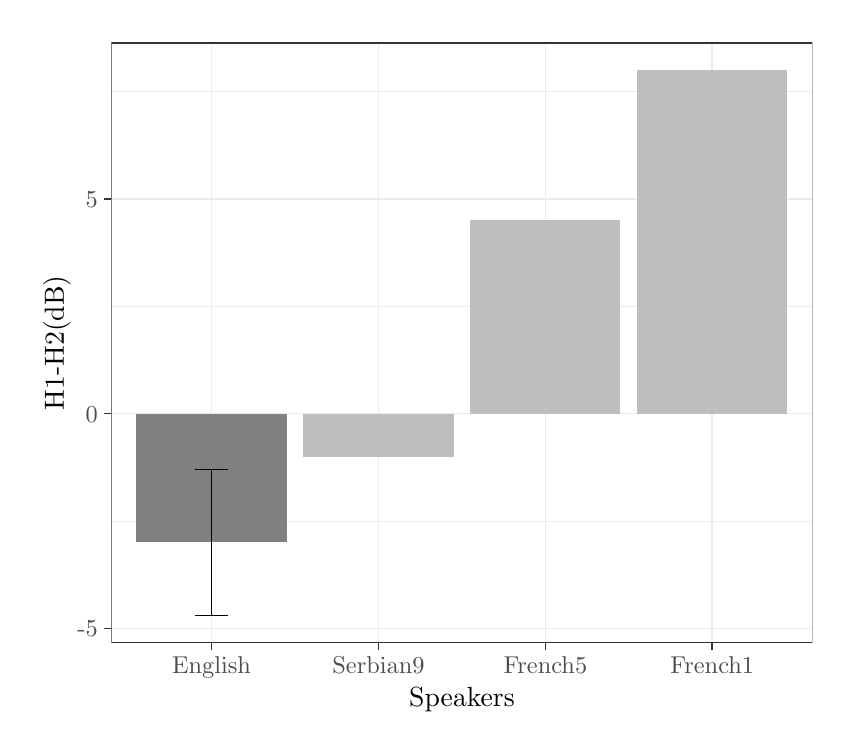
\begin{tikzpicture}[x=1pt,y=1pt]
\definecolor{fillColor}{RGB}{255,255,255}
\path[use as bounding box,fill=fillColor,fill opacity=0.00] (0,0) rectangle (289.08,252.94);
\begin{scope}
\path[clip] (  0.00,  0.00) rectangle (289.08,252.94);
\definecolor{drawColor}{RGB}{255,255,255}
\definecolor{fillColor}{RGB}{255,255,255}

\path[draw=drawColor,line width= 0.6pt,line join=round,line cap=round,fill=fillColor] (  0.00,  0.00) rectangle (289.08,252.94);
\end{scope}
\begin{scope}
\path[clip] ( 30.25, 30.69) rectangle (283.58,247.45);
\definecolor{fillColor}{RGB}{255,255,255}

\path[fill=fillColor] ( 30.25, 30.69) rectangle (283.58,247.45);
\definecolor{drawColor}{gray}{0.92}

\path[draw=drawColor,line width= 0.3pt,line join=round] ( 30.25, 74.67) --
	(283.58, 74.67);

\path[draw=drawColor,line width= 0.3pt,line join=round] ( 30.25,152.25) --
	(283.58,152.25);

\path[draw=drawColor,line width= 0.3pt,line join=round] ( 30.25,229.83) --
	(283.58,229.83);

\path[draw=drawColor,line width= 0.6pt,line join=round] ( 30.25, 35.88) --
	(283.58, 35.88);

\path[draw=drawColor,line width= 0.6pt,line join=round] ( 30.25,113.46) --
	(283.58,113.46);

\path[draw=drawColor,line width= 0.6pt,line join=round] ( 30.25,191.04) --
	(283.58,191.04);

\path[draw=drawColor,line width= 0.6pt,line join=round] ( 66.44, 30.69) --
	( 66.44,247.45);

\path[draw=drawColor,line width= 0.6pt,line join=round] (126.75, 30.69) --
	(126.75,247.45);

\path[draw=drawColor,line width= 0.6pt,line join=round] (187.07, 30.69) --
	(187.07,247.45);

\path[draw=drawColor,line width= 0.6pt,line join=round] (247.39, 30.69) --
	(247.39,247.45);
\definecolor{fillColor}{gray}{0.50}

\path[fill=fillColor] ( 39.29, 66.92) rectangle ( 93.58,113.46);
\definecolor{fillColor}{RGB}{190,190,190}

\path[fill=fillColor] ( 99.61, 97.95) rectangle (153.90,113.46);

\path[fill=fillColor] (159.93,113.46) rectangle (214.21,183.29);

\path[fill=fillColor] (220.25,113.46) rectangle (274.53,237.59);
\definecolor{drawColor}{RGB}{0,0,0}

\path[draw=drawColor,line width= 0.6pt,line join=round] ( 60.40, 93.29) --
	( 72.47, 93.29);

\path[draw=drawColor,line width= 0.6pt,line join=round] ( 66.44, 93.29) --
	( 66.44, 40.54);

\path[draw=drawColor,line width= 0.6pt,line join=round] ( 60.40, 40.54) --
	( 72.47, 40.54);

\definecolor{drawColor}{gray}{0.20}

\path[draw=drawColor,line width= 0.6pt,line join=round,line cap=round] ( 30.25, 30.69) rectangle (283.58,247.45);
\end{scope}
\begin{scope}
\path[clip] (  0.00,  0.00) rectangle (289.08,252.94);
\definecolor{drawColor}{gray}{0.30}

\node[text=drawColor,anchor=base east,inner sep=0pt, outer sep=0pt, scale=  0.88] at ( 25.30, 32.85) {-5};

\node[text=drawColor,anchor=base east,inner sep=0pt, outer sep=0pt, scale=  0.88] at ( 25.30,110.43) {0};

\node[text=drawColor,anchor=base east,inner sep=0pt, outer sep=0pt, scale=  0.88] at ( 25.30,188.01) {5};
\end{scope}
\begin{scope}
\path[clip] (  0.00,  0.00) rectangle (289.08,252.94);
\definecolor{drawColor}{gray}{0.20}

\path[draw=drawColor,line width= 0.6pt,line join=round] ( 27.50, 35.88) --
	( 30.25, 35.88);

\path[draw=drawColor,line width= 0.6pt,line join=round] ( 27.50,113.46) --
	( 30.25,113.46);

\path[draw=drawColor,line width= 0.6pt,line join=round] ( 27.50,191.04) --
	( 30.25,191.04);
\end{scope}
\begin{scope}
\path[clip] (  0.00,  0.00) rectangle (289.08,252.94);
\definecolor{drawColor}{gray}{0.20}

\path[draw=drawColor,line width= 0.6pt,line join=round] ( 66.44, 27.94) --
	( 66.44, 30.69);

\path[draw=drawColor,line width= 0.6pt,line join=round] (126.75, 27.94) --
	(126.75, 30.69);

\path[draw=drawColor,line width= 0.6pt,line join=round] (187.07, 27.94) --
	(187.07, 30.69);

\path[draw=drawColor,line width= 0.6pt,line join=round] (247.39, 27.94) --
	(247.39, 30.69);
\end{scope}
\begin{scope}
\path[clip] (  0.00,  0.00) rectangle (289.08,252.94);
\definecolor{drawColor}{gray}{0.30}

\node[text=drawColor,anchor=base,inner sep=0pt, outer sep=0pt, scale=  0.88] at ( 66.44, 19.68) {English};

\node[text=drawColor,anchor=base,inner sep=0pt, outer sep=0pt, scale=  0.88] at (126.75, 19.68) {Serbian9};

\node[text=drawColor,anchor=base,inner sep=0pt, outer sep=0pt, scale=  0.88] at (187.07, 19.68) {French5};

\node[text=drawColor,anchor=base,inner sep=0pt, outer sep=0pt, scale=  0.88] at (247.39, 19.68) {French1};
\end{scope}
\begin{scope}
\path[clip] (  0.00,  0.00) rectangle (289.08,252.94);
\definecolor{drawColor}{RGB}{0,0,0}

\node[text=drawColor,anchor=base,inner sep=0pt, outer sep=0pt, scale=  1.00] at (156.91,  7.64) {Speakers};
\end{scope}
\begin{scope}
\path[clip] (  0.00,  0.00) rectangle (289.08,252.94);
\definecolor{drawColor}{RGB}{0,0,0}

\node[text=drawColor,rotate= 90.00,anchor=base,inner sep=0pt, outer sep=0pt, scale=  1.00] at ( 13.08,139.07) {H1-H2(dB)};
\end{scope}
\end{tikzpicture}

  %\includegraphics[width=0.75\textwidth]{figures/phonation.png}
    \caption{Voice Quality Comparisons between L1 and L2 Productions of /ɪ/}
    \label{fig:h1h2}
  \figSpace
\end{figure}

Figure \ref{fig:h1h2} shows the average H1-H2 values of L1 and L2 segments. The three L2 speech samples involving the raising of [ɪ] in “\textit{six}” were all produced by females. Therefore, the comparison below illustrates only the difference between the three female L2 productions and all female L1 productions. As the figure shows, all three L2 speakers’ pronunciation had a relatively higher degree of breathiness (i.e., higher H1-H2 values) than the L1 speaker norm. The Serbian speaker’s production is less breathy than the other two L2 speakers; it is nevertheless breathier than the native mean. The fact that the SAA transcribers perceived high vowels with breathy quality as [i] is consistent with previous findings on the effect of voice quality on vowel height perception \citep{Lotto_1997}. The IPA transcriptions for these L2 speech samples were therefore accepted by the current study to represent vowel tensing. 



\subsection{Summary of Segmental Analysis}

The current study selected four types of L2 speech samples. Stimuli selection was based on IPA transcriptions available in the SAA. The most common L1 productions in the SAA were considered the L1 target productions. L2 speech samples that were transcribed the same as their L1 target productions were termed as the match stimuli. L2 speech samples whose IPA transcriptions differ from transcriptions of their L1 target productions were termed as the mismatch stimuli. The sections above described two types of mismatch stimuli. The first type consists of 25 L2 speech samples that were termed consonant mismatch. IPA transcriptions for these L2 speech samples differ from their L1 target productions by only one consonant. The second type consists of 25 L2 speech samples that were termed vowel mismatch. IPA transcriptions for these L2 speech samples differ from their L1 target productions by only one vowel. 

Acoustic analysis was conducted to examine the reliability of the IPA transcriptions. As shown in the analysis above, acoustic differences between the L2 speech samples and their corresponding L1 speech samples could be captured by IPA transcriptions of the L2 speech samples. The current study, therefore, considered these IPA transcriptions reliable. Audio files of these L2 speech samples were thus used by the current study as stimuli in two perception studies (Chapters 4 and 5). 

The third type of mismatch was termed syllable mismatch, because it concerns syllable structure differences between an L2 speech sample and its L1 target production. While consonant or vowel changes preserve the original syllable structure, segment deletion or segment epenthesis changes the original structure. The next section describes the selection of the 25 speech samples with syllable mismatches.

\subsection{Syllable Structures}

Structural variations investigated by the current study involve vowel epenthesis and consonant deletion. Co-articulatory properties and/or L1 phonotactics could, to some degree, generate a perceptual illusion of segment insertion, often termed as the “ghost segments” or “illusory segments” \citep{Dupoux_1999}. To select stimuli with potential structural problems, L2 audio samples were inspected in PRAAT to rule out possible cases of illusory perception. The following section uses two examples to illustrate how the inspections were carried out. As mentioned previously, the most common L1 productions in the SAA were considered representatives of L1 target productions. For example, the majority of the 100 surveyed L1 speakers of American English pronounced the word “\textit{ask}” in phrase “\textit{ask her}” as [æsk], while only one of the 100 L1 speakers pronounced the “\textit{ask}” as [æs]. [æsk] was therefore considered the L1 target production. [æs] was considered as a production with syllable mismatch. In other words, productions with mismatches are uncommon in L1 speech, but they are not necessarily unique to L2 speakers. 

To select L2 speech samples whose syllable structure differ from L1 target productions, the current study selected 25 L2 speech samples from the SAA based on their respective IPA transcriptions. To further inspect the reliability of the IPA transcriptions, acoustic information of the L2 speech samples were examined in PRAAT. If spectral information of a segment was missing from an L2 speech sample but existed in L1 target productions, then the L2 speech sample was considered as a stimulus with syllable mismatch. More specifically, it was considered a stimulus with segment deletion. Alternatively, if spectral information of a segment existed in an L2 speech sample but was missing from L1 target productions, then the L2 speech sample was considered as a stimulus with segment insertion.

\subsubsection{Segment Deletion}

Figure \ref{fig:del} shows the spectrogram of an L1 production and an L2 production of “\textit{ask her}”, where the dotted lines represent pitch contours and the solid lines represent intensity contours. The graph on the left illustrates an L1 production, which shows visible stop closure and burst after /s/. These characteristics are absent from the L2 production on the right, indicating that coda /k/ was dropped by the L2 speaker.

\begin{figure}[h!]
  \figSpace
    \centering
	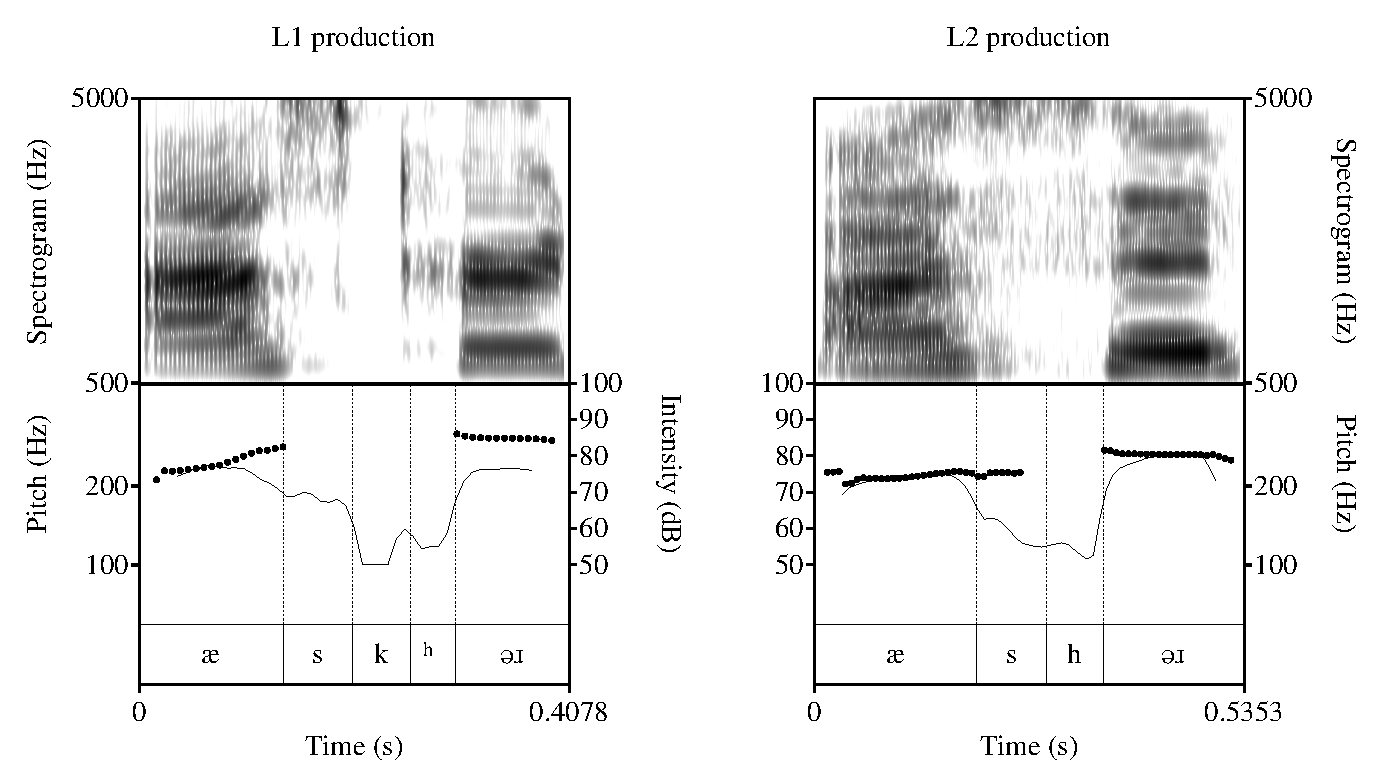
\includegraphics[width=1\textwidth]{figures/chp3/kdel.eps}
    \caption{/k/-Deletion in “\textit{ask her}”}
    \label{fig:del}
  \figSpace
\end{figure}

\subsubsection{Segment Insertion}

Eight stimuli were included in the current study to represent three types of segment insertions. Two stimuli involved prothesis of s-clusters (i.e., [sp]$\rightarrow$[əsp] in “\textit{six spoons}”); three stimuli involved anaptyxis of /pl/-clusters (i.e., /pl/ to /pəl/ in “\textit{please call}”); two stimuli represent paragoge at the end of “\textit{ask}” (i.e., [æsk]$\rightarrow$[æskə]), and one stimulus represents paragoge at the end of “five” (i.e. [faɪv] to [faɪvə]). The SAA transcribers marked discourse fillers and epenthetic vowels differently. A space was added between discourse fillers and their adjacent segments (e.g., [æsk ə həɹ]). No space was added between epenthetic vowels and the segment they epenthesize to (e.g., [æskə həɹ]). Speech samples with discourse fillers were not selected. The eight stimuli all contain epenthetic vowels as indicated by their respective IPA transcriptions. 

Figure \ref{fig:epen} illustrates a case of paragoge. The speech sample was produced by a Korean speaker who inserted a /ə/-like vocoid at the end of the word “\textit{ask}.” The epenthesized vocoid was transcribed by the SAA transcribers as a [ə]. 

\begin{figure}[h!]
  \figSpace
    \centering
	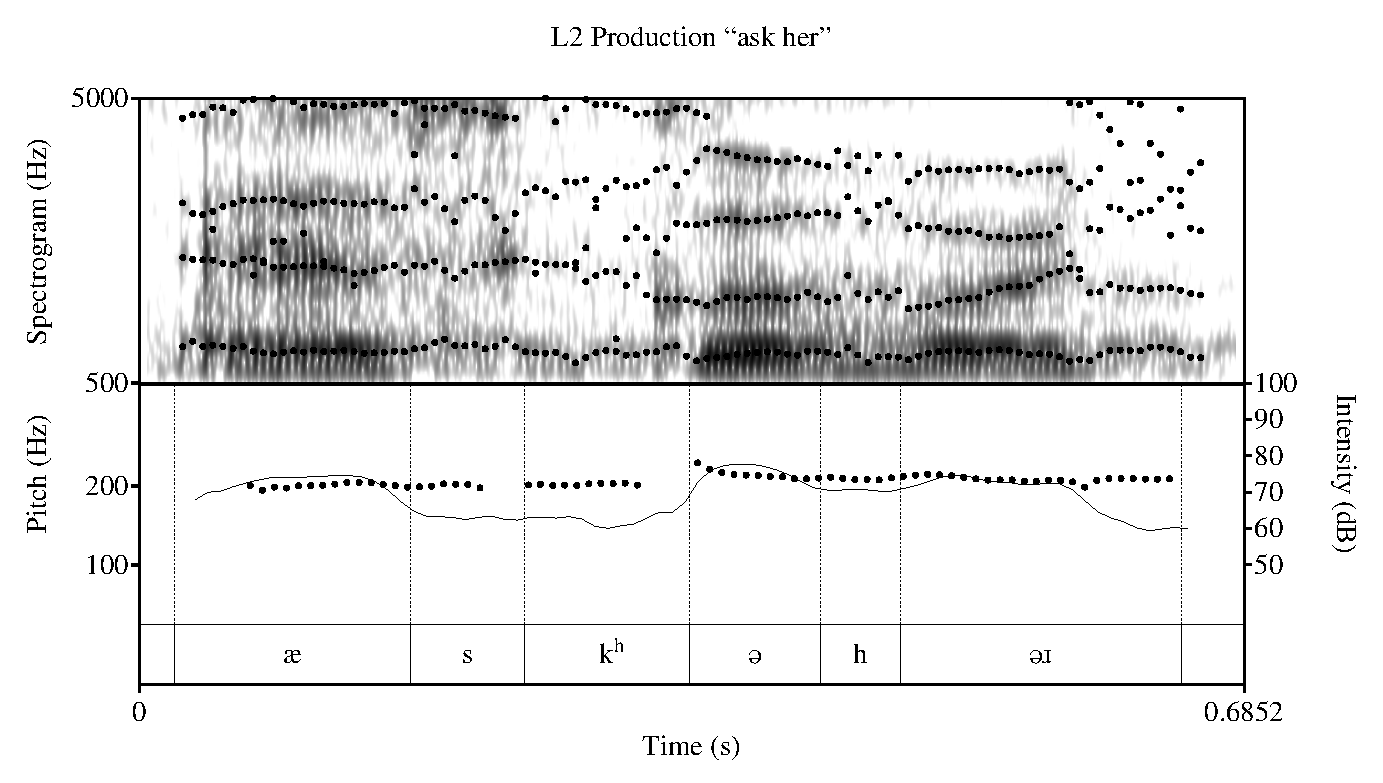
\includegraphics[width=0.8\textwidth]{figures/chp3/insert.eps}
    \caption{Paragoge after “\textit{ask}”}
    \label{fig:epen}
  \figSpace
\end{figure}

Spectral inspection carried out by the current study has successfully identified the epenthesized vocoid because it shows clear formant structures, carries pitch, and contains an intensity peak. These characteristics were utilized in the inspection of all other cases of segment insertion. Of the eight cases inspected, seven of them satisfy the aforementioned criteria. The prothetic vocoid of /sp/ does not carry pitch, yet it contains clear formant structures and an intensity peak. One could argue against defining such vocoid, and indeed all the other seven vocoids, as epenthetic vowels. As previous research often shows, epenthetic vowels, transitional vowels and extended sonorants are sometimes difficult to distinguish, and definitions of epenthetic vowels vary from language to language \citep{Gouskova_2009, Hall_2011, Hall_2003}. 

The current study took an impressionistic approach with regard to vowel epenthesis. As long as the epenthesized segment has clear formant structure and was transcribed with a [ə] or [ɪ], it is considered an epenthetic vocoid.  In summary, IPA transcriptions of the 25 L2 speech samples were verified via the process discussed above. The 25 L2 speech samples were selected as stimuli with syllable mismatches. 

\section{Summary}

The current study selected 100 L2 speech samples as stimuli in two perception studies. The L2 speech samples were chosen based primarily on their IPA transcriptions in the SAA. To observe the potential effects of phonological context on accentedness perception, five phonological contexts from the so-called “Stella” passage were chosen. Each context was represented by 20 L2 speech samples, yielding 100 L2 speech samples in total. To determine the L1 target productions for the five contexts, IPA transcriptions of 100 L1 speakers of American English from the SAA were surveyed to find the most common productions (e.g., [pʰliz kʰɑl] for “\textit{please call}”). L2 speech samples that were transcribed the same as their L1 target productions were termed as the match stimuli. L2 speech samples that were not transcribed as the same as their L1 target productions were termed as the mismatch stimuli. 

Among the 20 L2 speech samples for each of the five contexts, five speech samples were the match stimuli (e.g., [pʰliz kʰɑl] for “\textit{please call}”). The rest 15 L2 speech samples were the mismatch stimuli. Among the 15 mismatch stimuli, five differed from their L1 target production by only one consonant (e.g., [pʰlis kʰɑl] for “\textit{please call}”), five differed from their L1target production by only one vowel (e.g., [pʰliz kʰol] for “\textit{please call}”). Another five L2 speech samples, did not differ from their L1 target production segmentally, but contained either one more or one less segment than their L1 target productions (e.g., [pʰəliz kʰɑl] or [pʰliz kʰɑ] for “\textit{please call}”). These three types of stimuli were termed consonant mismatch, vowel mismatch, and syllable mismatch respectively. 

To verify the reliability of the IPA transcriptions for the 100 L2 stimuli, acoustic analysis was performed to compare L2 speech samples with their L1 counterparts. Speech samples from 50 L1 speakers of American English were extracted from the SAA for the analysis of native speaker pronunciation norms, which were approximated by the mean L1 values of relevant benchmark acoustic measurements (e.g., mean L1 VOT duration, mean L1 COG, mean L1 F1/F2/F3 values etc.). Results showed that acoustic differences between the L2 stimuli and native speaker norms were successfully captured by the IPA transcriptions. The current study therefore concluded that these IPA transcriptions for the 100 L2 stimuli are reliable. These stimuli were then used in two perception studies to elicit accentedness judgment from L1 listeners of American English. 

































\chapter{Experiment 1}
\label{ch:4}

\section{Introduction}

Experiment 1 of the current study investigates the accentedness of various phonetic patterns in non- native (L2) English speech. The current study considers the most common native (L1) English productions observed in one hundred L1 speakers of American English as the L1 target productions (e.g., [æsk] for “\textit{ask}”). L2 speech productions that differ from the L1 target productions were considered mismatches. The mismatch stimuli, therefore, represent patterns in L2 speech that do not match the most common L1 productions.

Eleven types of consonant mismatches, 5 types of vowel mismatches and 2 types of syllable structure mismatches were assembled to enable a detailed comparison between different types of speech patterns in L2 speech. The stimuli were chosen based on their phonetic transcriptions (IPA transcriptions), which were vetted by at least 3 professional transcribers and were further examined by acoustic analysis conducted by the current study, as described in Chapter \ref{ch:3}.

L1 American English raters were recruited from the Amazon Mechanical Turk (MTurk) platform to provide accentedness judgments on the stimuli. The results provide direct comparisons between the accentendess of different types of consonant, vowel and syllable structural patterns in L2 speech.


\section{Stimuli}

Stimuli for the current study were selected based on their respective phonetic transcriptions, which were verified by acoustic analysis conducted as part of the current study (Chapters \ref{ch:3}). An example of the four types of stimuli were introduced in Chapter \ref{ch:3} and are re-listed here in Table 4.1, where the “Contexts” column specifies the five phonological contexts. There are 20 stimuli for each of the 5 contexts, yielding 100 stimuli in total.

% Table generated by Excel2LaTeX from sheet 'stimuli'
\begin{table}[!h]
  \figSpace
  \centering
  \caption{Types of Stimuli}
\label{table:tos2}
    \begin{tabular}{p{5.2em}llll}
    \toprule
    Contexts & \multicolumn{1}{p{5.2em}}{Match} & \multicolumn{1}{p{5em}}{Consonant\quad Mismatch} & \multicolumn{1}{p{5em}}{Vowel\quad Mismatch} & \multicolumn{1}{p{5em}}{Syllable\quad Mismatch} \\
    \midrule
    \textit{please call} &[pʰliz kʰɑl]&[\textbf{p}liz kʰɑl]&[pʰliz kʰ\textbf{o}l]&[pʰ\textbf{ə}liz kʰɑl] \\
     \textit{ask her} &[æsk (h)əɹ] &[æsk hə\textbf{r}]&[\textbf{ɑ}sk həɹ]&[æs\underline{ } həɹ]\\
     \textit{six spoons} &[sɪks spunz]&[sɪks spun\textbf{ʃ}]&[s\textbf{i}ks spunz]&[sɪks \textbf{ə}spunz] \\
     \textit{five thick} &[faɪv θɪk]&[faɪv \textbf{t}ɪk] &[f\textbf{a}v θɪk]&[faɪv\textbf{ə} θɪk]\\
     \textit{small plastic} &[smɑl pʰlæstɪk]&[smɑ\textbf{ɭ} pʰlæstɪk]&[smɑl pʰlæst\textbf{i}k]&[smɑl pʰlæs\underline{ }ɪk] \\
    \bottomrule
    \end{tabular}%
      \figSpace
\end{table}%

IPA transcriptions of the match stimuli are the same as IPA transcriptions of their L1 target productions (e.g.  [θɪk] for “\textit{thick}”), meaning that the IPA transcriptions of the match stimuli match IPA transcriptions of their L1 target productions. L2 speech samples that do not match their L1 target productions were termed the mismatch stimuli. The mismatch stimuli were further divided into three groups based on three types of mismatches, namely, stimuli with consonant mismatches (e.g., [tɪk] for “\textit{thick}”), stimuli with vowel mismatches (e.g., [θik] for “\textit{thick}”), and stimuli with syllable structure mismatches (e.g., [faɪvə] for “\textit{five}”). Experiment 1 therefore investigates four types of stimuli (i.e., the match stimuli and the three types of mismatch stimuli).


\section{Procedure}
 
Experiment 1 recruited L1 listeners of American English to provide accentedness ratings of the 100 stimuli. Participants (i.e., raters) heard each of the 100 audio stimuli and were then asked to judge the degree of the foreign accent exhibited in the stimulus on a 9-point Likert-like scale (Figure \ref{fig:exp1}). Following the practice of similar studies (e.g., McCullough, 2013), only the endpoints of the scale were marked. 

The raters heard the 100 audio stimuli without knowing the intended meaning of the stimuli. A rating of one means the stimulus has no foreign accent at all. A rating of nine means the stimulus has a very strong foreign accent.

The interface of the experiment provided a button and a 9-point rating scale. Raters were instructed to wear headphones or earbuds to listen to the stimuli\footnote{Since the experiment was conducted online, we cannot ensure that all the raters wore headphones or earbuds during the experiment. This could be a potential methodological limitation. Readers could consult \citet{Woods_2017} for a psychophysical test that helps to determine whether online experiment participants are wearing headphones.}. A stimulus was played once the rater hit the button, after which the rating scale would appear. Raters provided their accentedness judgment by choosing a number from one to nine on the rating scale, and then moved on to the next trial. There was no time limit for each trial. The maximum time allowed for completing the entire experiment was 30 minutes. Figure \ref{fig:exp1} illustrates the interface of the experiment.

\begin{figure}[!h]
  \figSpace
    \centering
	\includegraphics[width=0.75\textwidth]{figures/exp1.jpg}
    \caption{Interface of Experiment 1}
    \label{fig:exp1}
  \figSpace
\end{figure}

To reduce the order-effect, a block randomization technique was implemented. The 100 stimuli were divided into five blocks, each of which contained one token per type per context, yielding 20 stimuli per block (five contexts × four types). The order of blocks and the stimuli in each block were randomized for each participant via JavaScript using the Fisher-Yates Shuffle algorithm \citep{Fisher_1963}. 

 Raters of Experiment 1 were not required to identify or locate the specific type of mismatch in each stimulus, because the mismatch had already been determined by the vetted transcriptions.

There were 100 trials in total. At the end of the experiment, the raters were asked to take a demo- graphics survey, which collected information on the raters’ age, gender, L1/L2 status, occupation, current residence and birthplace. Raters on average spent 12.3 minutes (SD=3.2 minutes) on the experiment. Raters were compensated \$0.50 upon completion of the experiment. The experiment was programmed with HTML, CSS and JavaScript.

Previous studies often provide a training session to familiarize participants with the range of accents in the experiment \citep{Major_1986, Munro_1999}. However, the conundrum is that there is no way to obtain the full range of accents without testing the raters first. Experimenters could subjectively select a few representative stimuli for the training session, but ex- perimenters’ own biases could be introduced in the process. Experiment 1 therefore opted to omit the training session. The Result section of this chapter discusses how the absence of training affects raters’ accentedness judgments.


\section{Raters}
\label{rater:1}
Participants (i.e., raters) were 110 adult L1 American English speakers recruited via Amazon Me- chanical Turk (MTurk), a web-application that allows researchers to conduct survey-based experi- ments. Previous literature has shown that results of behavioral experiments conducted on MTurk are comparable to results of similar experiments conducted in lab settings \citep{Enochson_2015, Sprouse_2010}. \citet{Difallah_2018} recently showed that there are about 2,000 participants active on MTurk at any given time. 51\% of them are female, 49\% of them are male. About 75\% of the participants are from the United States. Indian participants represent 16\% of the population. The rest are from Canada, Great Britain, the Philippines and Germany.

Since Experiment 1 aims to investigate accentedness judgments of American English listeners, the experiment was made accessible only to people with a U.S. IP address. To increase the reliability of responses, the experiment required participants to have an approval rating of at least 95\%. That is, at least 95\% of each participant’s previous work on MTurk has met the requirements of the people who assigned the work.  All of the participants reported their birth location and residence as being in the United States. All of them reported that that they are L1 speakers of English. We therefore assumed that the participants are L1 speakers of American English. Two of the participants reported having speech or hearing related disorders. Responses from these two participants were thus removed, yielding 108 participants in total, among which 61 were female, 45 were male, and two did not report their gender. The age of the 108 participants ranged from 20 to 66. The mean age was 33.50 (SD=12.51) (See rater demographics in Appendix B).

\section{Control for Prosody}
\label{ch4:prosody}

The current study focuses specifically on segmental and syllable structure information. However, prosodic information has often been shown to affect foreign accent perception (e.g., \citealp{Magen_1998, Munro_1995}). It is therefore important for the current study to control for prosodic information of the selected stimuli. The following section first reviews the methods used by previous studies and then describes the method implemented by the current study.

 Two types of methods were often used in previous research to account for prosodic information. One method, usually termed \textit{prosody cloning} or \textit{prosody transplantation}, involves the superimposing of prosody of one utterance onto another \citep{Mareuil_2006, Yoon_2007}. At least two utterances are required with this method. Usually, highly controlled read speech samples are used, so that the two utterances contain exactly the same number of segments. The duration, fundamental frequency (F0), or intensity of segments in one utterance (the “donor”) can be automatically superimposed on the other utterance (the “recipient”) via the PSOLA algorithm \citep{Moulines_1990}. In this way, the recipient sample may have similar or even identical prosodic characteristics as the donor. 

The drawback of this method is that the number of segments in the donor and the recipient should be the same, which might cause problems for imposing L1 prosody on L2 speech with epenthesis or segment deletion. Moreover, acoustic manipulations of prosody will probably alter the acoustic characteristics in segmental dimensions, which might artificially increase or decrease accentedness of the original speech. Therefore, it might not be ideal to implement this method in studies that investigate segmental characteristics of foreign accent. 

An alternative method measures the prosodic differences without acoustic manipulation. This method implements the Dynamic Time Warping (DTW) alignment algorithm to account for the prosodic difference between two utterances \citep{Adami_2003, Rilliard_2011, Sharpe_2015}. DTW is a non-linear algorithm that looks for the dissimilarity between two temporal sequences of data and calculates the costs to align one with the other.  It generates a DTW score that represents the dissimilarity between two sets of data. The greater the DTW score, the more dissimilar the two sets of data are. 

The advantages of the DTW method are that (1) it does not involve any acoustic manipulation of the original speech files; (2) it does not require that the two utterances compared contain the same number of segments, which make it suitable for comparing L1 and L2 speech samples that differ in syllable structure; and (3) the calculation not only compares F0 and/or intensity values at different time points, but also takes into account the durational difference between two utterances, where larger differences will lead to a greater DTW score. In other words, the DTW score might, to some degree, represent the global prosodic differences of two utterances. The DTW method could thus be more suitable for the current study. 

In the current study, the DTW algorithm took F0 values of L1 speech samples as the reference and F0 values of an L2 speech sample as the input. The algorithm generated DTW scores, which represent the intonational and durational dissimilarities between the L1 and L2 speech samples.  L1 productions were first analyzed to find L1 F0 contours. Male and female speech samples were separately processed. For each gender, speech samples were grouped by the five contexts. F0 contours of the speech samples were extracted using the PRAAT auto-correlation algorithm \citep{Boersma_2015}. The contours were then divided into 300 equally spaced time points for every second (i.e., 3.33 ms per point), from which an F0 value was extracted. Following \citet{Morrill_2015}, gaps in the contour were interpolated from the points on either side of the gap. Artifacts were removed by smoothing with a bandwidth of 5 Hz. F0 values were then converted to semitones relative to 100 Hz. Pitch range for female speech samples was set between 100 Hz and 500 Hz. Pitch range for male speech samples was set between 75 Hz and 300 Hz. To allow for cross-speaker comparison, the semitones were then normalized for each speaker. 

F0 values of the 100 L2 stimuli were similarly extracted and normalized. The DTW algorithm was then implemented in R with the \textit{dtw} package \citep{Giorgino_2009} to calculate the degree of prosodic dissimilarity between L1 and L2 speech samples. For every L2 stimulus, 25 DTW scores were generated to represent the warping cost between the L2 stimulus and each of its corresponding 25 L1 speech samples. The mean DTW scores for each L2 stimulus were then calculated to account for prosodic information of the stimulus. The mean DTW scores for all of the 100 L2 stimuli were recorded for further statistical analysis. 

\section{Results}
\subsection{Experiment 1 Hypotheses}
Based on previous research on speech perception and lexical identification, Experiment 1 hypothesizes that stimuli with consonant mismatches are perceptually more foreign-accented than stimuli with vowel mismatches, because consonants are more susceptible to categorical perception than vowels and are more important in lexical identification. Based on previous empirical findings on L2 speech perception, Experiment 1 predicts that segment epenthesis is perceptually more foreign-accented than segment deletion, because segment deletion is sometimes allowed in L1 speech, while segment epenthesis rarely occurs. Experiment 1 also predicts that stimuli with mismatches should be generally more foreign-accented than stimuli without mismatches (i.e., the match stimuli).

\subsection{Segmental and Structural Mismatches}

The mean ratings across all four stimulus types (each stimulus was rated on a scale from 1 to 9) was 4.81 (SD=2.21). The larger the number, the more foreign-accented a stimulus was judged. As expected, raters assigned higher ratings for stimuli with mismatches (M=5.10, SD=2.15) than for stimuli without mismatches (M=3.94, SD=2.16). Ratings of stimuli with consonant mismatches (M=5.66, SD=2.04) were on average higher than ratings of stimuli with syllable structural mismatches (M=4.96, SD=2.17), which were on average higher than ratings of stimuli with vowel mismatches (M=4.69, SD=2.13). Figure \ref{fig:bar1} demonstrates the mean ratings of the four types of stimuli, where the error bars represent the 95\% confidence intervals. 

\begin{figure}[!h]
  \figSpace
\centering
%bar1 for Exp1
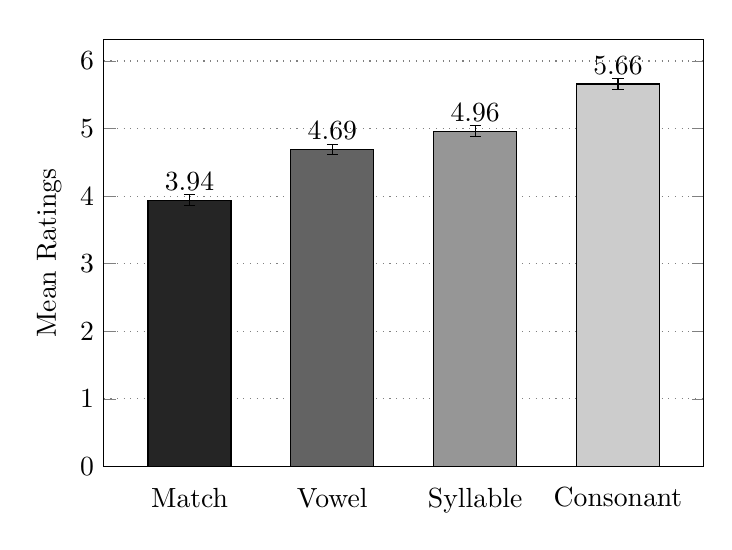
\begin{tikzpicture}
  \begin{axis}[
  ylabel={Mean Ratings},
width=9.2cm,
   height = 7cm,
    ytick distance=1,
        nodes near coords,
      major x tick style = transparent,
    ybar=3*\pgflinewidth,
      bar width=30pt,
      ymajorgrids = true,
      symbolic x coords={Match,Vowel,Syllable,Consonant},
      xtick ={Match,Vowel, Syllable, Consonant},
      scaled y ticks = false,
        legend style={at={(1.2,0.55)},
  anchor=north},
  legend cell align=left,
      enlarge x limits=0.20,
      ymin=0,
       every axis plot/.append style={
          ybar,
          bar shift=0pt,
          fill
        }
    ]
\addplot [fill=mycolor4,error bars/.cd, y dir=both, y explicit,error bar style=black] 
  coordinates {
          (Match, 3.94) += (0,0.08) -= (0,0.08)};
\addplot [fill=mycolor3,error bars/.cd, y dir=both, y explicit,error bar style=black] 
  coordinates {
          (Vowel, 4.69) += (0,0.08) -= (0,0.08)};
\addplot [fill=mycolor2,error bars/.cd, y dir=both, y explicit,error bar style=black] 
  coordinates {
          (Syllable, 4.96) += (0,0.08) -= (0,0.08)};
 \addplot [fill=mycolor1,error bars/.cd, y dir=both, y explicit,error bar style=black] 
  coordinates {
          (Consonant, 5.66) += (0,0.08) -= (0,0.08)};
 \end{axis}
\end{tikzpicture}



\caption{Mean Ratings by Type of Stimuli on the Scale from 1 to 9}
\label{fig:bar1}
\figSpace
\end{figure}

Linear mixed-effects models were employed with the \textit{lme4} package in R \citep{Bates_2014} to investigate the possible influence of the segmental and syllable mismatches on foreign accent ratings. In the full model, the dependent variable was the ratings. Type of stimuli (consonant mismatch vs. vowel mismatches vs. syllable mismatch vs. match) was Helmert contrast-coded to examine whether the four types of stimuli affect accentedness rating differently. Three stimuli contrasts were created. The first contrast compared consonant mismatch with syllable mismatch; the second contrast compared vowel mismatch with consonant and syllable mismatch; and the third contrast compared the three types of mismatch stimuli with the match stimuli. To investigate accentedness ratings across the 100 trials, trial numbers were also included as a fixed effect. To control for prosody, the mean DTW score of each stimulus was included as a fixed effect. The interactions among the three stimuli contrasts, the trial number and the DTW scores were also included as fixed effects. Raters were included as a random effect with the “type of stimuli” as its random slope. Stimuli were included as another random effect.

The effects of fixed effect factors were investigated by comparing models using the likelihood ratio test. The full model was as described above. The likelihood ratio test is a test of the goodness-of-fit between two models. It produces a chi-square and a p-value to indicate whether one model fits a particular set of data significantly better than the other model. To investigate the contribution of a particular fixed effect to model fit, the fixed effect needs to be removed from the full model to construct a new model. The new model, therefore, differs from the full model only by the exclusion of one single parameter (i.e., the particular fixed effect factor). If the full model indeed fits the dataset significantly better than the new model, then one could conclude that the exclusion of the specific fixed effect factor significantly changed the model fit, which implies that the fixed effect factor in question is statistically significant. 

To investigate the effect of DTW scores, the fixed effect factor DTW cores was removed from the full model to construct a new model.  The new model was compared to the full model using the likelihood ratio test. The result showed that the full model did not fit the dataset significantly better than the new model (χ2 = 2.87, p =.09), indicating that the contribution of DTW scores to model fit was not significant. The same method was applied to the investigation on other fixed effects. The results show that none of the interactions involving DTW scores achieved significant contribution to model fit, suggesting that the intonation of the stimuli might not be a major factor affecting accentedness ratings. 

The contrast between consonant and syllable mismatches significantly contributed to model fit (χ2 = 6.35, p < .05), showing that stimuli with consonant mismatches were rated as being more accented than stimuli with syllable mismatches. The second contrast, which compares vowel mismatches with consonant and syllable mismatches, contributed significantly to model fit (χ2 = 6.95, p < .01), showing that stimuli with consonant mismatches and syllable mismatches were rated as being more accented than stimuli with vowel mismatches. The third contrast, which compares the match stimuli with the three types of mismatch stimuli, also contributed significantly to model fit (χ2 = 13.32, p < .001), showing that stimuli with segmental and structural mismatches were perceived as being more accented than the match stimuli. 

These results suggest that all of the three types of mismatches contributed to the perception of foreign accent. However, stimuli with consonant mismatches were perceived as being more accented than the other two. Among the three types of mismatches, stimuli with vowel mismatches were perceived to be the least accented. The DTW scores, which represent prosodic differences between L1 and L2 productions, positively correlated with accentedness ratings. The contribution of the DTW scores to model fit was only marginally significant, suggesting that prosodic influence might not be a major factor that affected accentedness ratings. 

\subsection{Ratings across Time}

The comparison of models also revealed a significant effect of trial numbers on accentedness ratings (β=0.03, χ2 = 46.80, p < .001), suggesting that ratings were not consistent across the 100 trials. That is, the same stimuli might receive different ratings depending on when it occurred during the experiment. More specifically, the later a stimulus occurred in the experiment, the more accented the stimulus was rated. The interaction between trial number and the third contrast contributed significantly to model fit (β=0.04, χ2 = 9.87, p < .01), showing that stimuli with segmental and structural mismatches became more accented than the match stimuli as the experiment progressed. Figure \ref{fig:trial1} demonstrates the accentedness rating across time, where the ribbons represent the 95\% confidence intervals. The accentedness ratings increased as the experiment progressed. 

\begin{figure}[h!]
  \figSpace
    \centering
% Created by tikzDevice version 0.12.3 on 2019-11-24 19:33:25
% !TEX encoding = UTF-8 Unicode
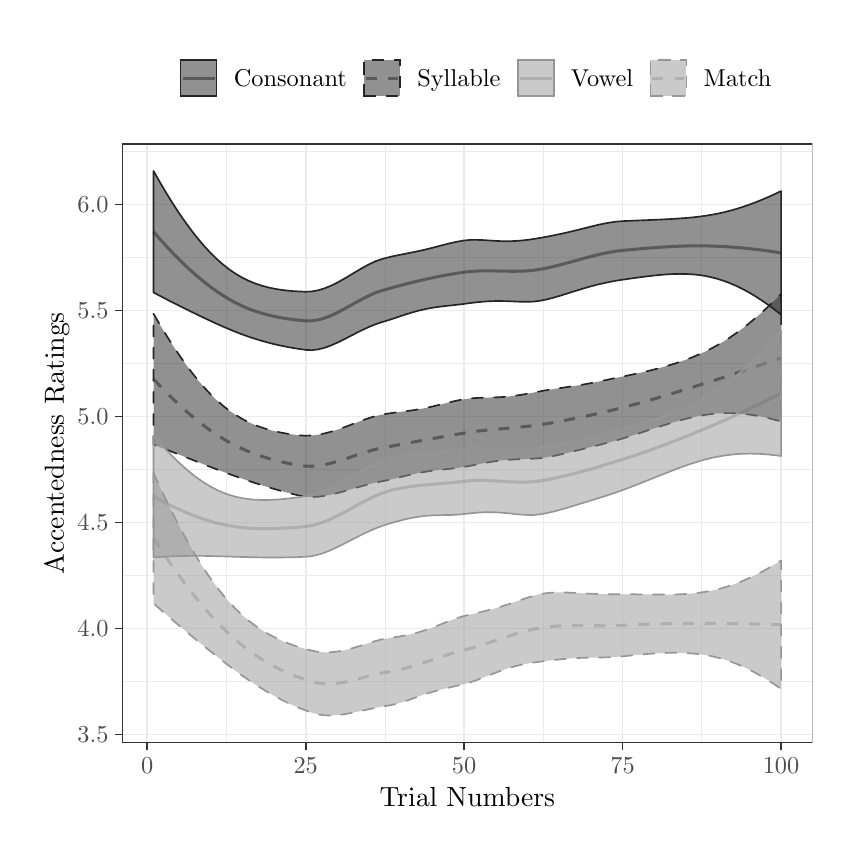
\begin{tikzpicture}[x=1pt,y=1pt]
\definecolor{fillColor}{RGB}{255,255,255}
\path[use as bounding box,fill=fillColor,fill opacity=0.00] (0,0) rectangle (289.08,289.08);
\begin{scope}
\path[clip] (  0.00,  0.00) rectangle (289.08,289.08);
\definecolor{drawColor}{RGB}{255,255,255}
\definecolor{fillColor}{RGB}{255,255,255}

\path[draw=drawColor,line width= 0.6pt,line join=round,line cap=round,fill=fillColor] (  0.00,  0.00) rectangle (289.08,289.08);
\end{scope}
\begin{scope}
\path[clip] ( 34.16, 30.69) rectangle (283.58,247.13);
\definecolor{fillColor}{RGB}{255,255,255}

\path[fill=fillColor] ( 34.16, 30.69) rectangle (283.58,247.13);
\definecolor{drawColor}{gray}{0.92}

\path[draw=drawColor,line width= 0.3pt,line join=round] ( 34.16, 52.87) --
	(283.58, 52.87);

\path[draw=drawColor,line width= 0.3pt,line join=round] ( 34.16, 91.17) --
	(283.58, 91.17);

\path[draw=drawColor,line width= 0.3pt,line join=round] ( 34.16,129.47) --
	(283.58,129.47);

\path[draw=drawColor,line width= 0.3pt,line join=round] ( 34.16,167.77) --
	(283.58,167.77);

\path[draw=drawColor,line width= 0.3pt,line join=round] ( 34.16,206.07) --
	(283.58,206.07);

\path[draw=drawColor,line width= 0.3pt,line join=round] ( 34.16,244.37) --
	(283.58,244.37);

\path[draw=drawColor,line width= 0.3pt,line join=round] ( 71.83, 30.69) --
	( 71.83,247.13);

\path[draw=drawColor,line width= 0.3pt,line join=round] (129.09, 30.69) --
	(129.09,247.13);

\path[draw=drawColor,line width= 0.3pt,line join=round] (186.35, 30.69) --
	(186.35,247.13);

\path[draw=drawColor,line width= 0.3pt,line join=round] (243.61, 30.69) --
	(243.61,247.13);

\path[draw=drawColor,line width= 0.6pt,line join=round] ( 34.16, 33.72) --
	(283.58, 33.72);

\path[draw=drawColor,line width= 0.6pt,line join=round] ( 34.16, 72.02) --
	(283.58, 72.02);

\path[draw=drawColor,line width= 0.6pt,line join=round] ( 34.16,110.32) --
	(283.58,110.32);

\path[draw=drawColor,line width= 0.6pt,line join=round] ( 34.16,148.62) --
	(283.58,148.62);

\path[draw=drawColor,line width= 0.6pt,line join=round] ( 34.16,186.92) --
	(283.58,186.92);

\path[draw=drawColor,line width= 0.6pt,line join=round] ( 34.16,225.22) --
	(283.58,225.22);

\path[draw=drawColor,line width= 0.6pt,line join=round] ( 43.20, 30.69) --
	( 43.20,247.13);

\path[draw=drawColor,line width= 0.6pt,line join=round] (100.46, 30.69) --
	(100.46,247.13);

\path[draw=drawColor,line width= 0.6pt,line join=round] (157.72, 30.69) --
	(157.72,247.13);

\path[draw=drawColor,line width= 0.6pt,line join=round] (214.98, 30.69) --
	(214.98,247.13);

\path[draw=drawColor,line width= 0.6pt,line join=round] (272.24, 30.69) --
	(272.24,247.13);
\definecolor{drawColor}{RGB}{37,37,37}

\path[draw=drawColor,draw opacity=0.50,line width= 1.1pt,line join=round] ( 45.49,215.33) --
	( 47.78,212.70) --
	( 50.07,210.17) --
	( 52.36,207.73) --
	( 54.66,205.39) --
	( 56.95,203.16) --
	( 59.24,201.04) --
	( 61.53,199.04) --
	( 63.82,197.15) --
	( 66.11,195.38) --
	( 68.40,193.73) --
	( 70.69,192.22) --
	( 72.98,190.83) --
	( 75.27,189.59) --
	( 77.56,188.49) --
	( 79.85,187.52) --
	( 82.14,186.67) --
	( 84.43,185.93) --
	( 86.72,185.30) --
	( 89.01,184.76) --
	( 91.30,184.31) --
	( 93.59,183.93) --
	( 95.88,183.62) --
	( 98.17,183.36) --
	(100.46,183.15) --
	(102.75,183.16) --
	(105.04,183.51) --
	(107.33,184.16) --
	(109.62,185.05) --
	(111.91,186.13) --
	(114.21,187.32) --
	(116.50,188.59) --
	(118.79,189.88) --
	(121.08,191.12) --
	(123.37,192.27) --
	(125.66,193.27) --
	(127.95,194.06) --
	(130.24,194.71) --
	(132.53,195.35) --
	(134.82,195.97) --
	(137.11,196.57) --
	(139.40,197.14) --
	(141.69,197.69) --
	(143.98,198.21) --
	(146.27,198.71) --
	(148.56,199.18) --
	(150.85,199.61) --
	(153.14,200.02) --
	(155.43,200.39) --
	(157.72,200.72) --
	(160.01,200.98) --
	(162.30,201.13) --
	(164.59,201.20) --
	(166.88,201.20) --
	(169.17,201.16) --
	(171.47,201.11) --
	(173.76,201.07) --
	(176.05,201.06) --
	(178.34,201.09) --
	(180.63,201.21) --
	(182.92,201.42) --
	(185.21,201.76) --
	(187.50,202.20) --
	(189.79,202.71) --
	(192.08,203.28) --
	(194.37,203.89) --
	(196.66,204.52) --
	(198.95,205.16) --
	(201.24,205.79) --
	(203.53,206.40) --
	(205.82,206.98) --
	(208.11,207.50) --
	(210.40,207.95) --
	(212.69,208.32) --
	(214.98,208.59) --
	(217.27,208.80) --
	(219.56,209.01) --
	(221.85,209.22) --
	(224.14,209.41) --
	(226.43,209.59) --
	(228.73,209.75) --
	(231.02,209.89) --
	(233.31,210.02) --
	(235.60,210.12) --
	(237.89,210.19) --
	(240.18,210.24) --
	(242.47,210.25) --
	(244.76,210.23) --
	(247.05,210.17) --
	(249.34,210.09) --
	(251.63,209.97) --
	(253.92,209.83) --
	(256.21,209.65) --
	(258.50,209.45) --
	(260.79,209.22) --
	(263.08,208.97) --
	(265.37,208.68) --
	(267.66,208.38) --
	(269.95,208.05) --
	(272.24,207.70);

\path[draw=drawColor,draw opacity=0.50,line width= 1.1pt,dash pattern=on 4pt off 4pt ,line join=round] ( 45.49,162.06) --
	( 47.78,159.65) --
	( 50.07,157.31) --
	( 52.36,155.05) --
	( 54.66,152.87) --
	( 56.95,150.79) --
	( 59.24,148.80) --
	( 61.53,146.91) --
	( 63.82,145.13) --
	( 66.11,143.46) --
	( 68.40,141.91) --
	( 70.69,140.48) --
	( 72.98,139.17) --
	( 75.27,137.98) --
	( 77.56,136.90) --
	( 79.85,135.92) --
	( 82.14,135.03) --
	( 84.43,134.23) --
	( 86.72,133.51) --
	( 89.01,132.86) --
	( 91.30,132.28) --
	( 93.59,131.76) --
	( 95.88,131.30) --
	( 98.17,130.88) --
	(100.46,130.62) --
	(102.75,130.60) --
	(105.04,130.80) --
	(107.33,131.18) --
	(109.62,131.71) --
	(111.91,132.35) --
	(114.21,133.07) --
	(116.50,133.84) --
	(118.79,134.62) --
	(121.08,135.38) --
	(123.37,136.08) --
	(125.66,136.70) --
	(127.95,137.20) --
	(130.24,137.63) --
	(132.53,138.05) --
	(134.82,138.48) --
	(137.11,138.91) --
	(139.40,139.33) --
	(141.69,139.75) --
	(143.98,140.17) --
	(146.27,140.59) --
	(148.56,141.00) --
	(150.85,141.40) --
	(153.14,141.80) --
	(155.43,142.20) --
	(157.72,142.59) --
	(160.01,142.94) --
	(162.30,143.25) --
	(164.59,143.52) --
	(166.88,143.76) --
	(169.17,143.97) --
	(171.47,144.17) --
	(173.76,144.37) --
	(176.05,144.57) --
	(178.34,144.79) --
	(180.63,145.03) --
	(182.92,145.30) --
	(185.21,145.60) --
	(187.50,145.96) --
	(189.79,146.36) --
	(192.08,146.77) --
	(194.37,147.20) --
	(196.66,147.65) --
	(198.95,148.11) --
	(201.24,148.59) --
	(203.53,149.09) --
	(205.82,149.61) --
	(208.11,150.13) --
	(210.40,150.68) --
	(212.69,151.24) --
	(214.98,151.81) --
	(217.27,152.40) --
	(219.56,153.01) --
	(221.85,153.64) --
	(224.14,154.29) --
	(226.43,154.95) --
	(228.73,155.62) --
	(231.02,156.31) --
	(233.31,157.01) --
	(235.60,157.71) --
	(237.89,158.42) --
	(240.18,159.14) --
	(242.47,159.86) --
	(244.76,160.58) --
	(247.05,161.30) --
	(249.34,162.03) --
	(251.63,162.77) --
	(253.92,163.51) --
	(256.21,164.27) --
	(258.50,165.03) --
	(260.79,165.80) --
	(263.08,166.58) --
	(265.37,167.37) --
	(267.66,168.17) --
	(269.95,168.98) --
	(272.24,169.81);
\definecolor{drawColor}{RGB}{150,150,150}

\path[draw=drawColor,draw opacity=0.50,line width= 1.1pt,line join=round] ( 45.49,119.69) --
	( 47.78,118.44) --
	( 50.07,117.24) --
	( 52.36,116.10) --
	( 54.66,115.03) --
	( 56.95,114.02) --
	( 59.24,113.07) --
	( 61.53,112.20) --
	( 63.82,111.41) --
	( 66.11,110.69) --
	( 68.40,110.07) --
	( 70.69,109.53) --
	( 72.98,109.08) --
	( 75.27,108.72) --
	( 77.56,108.44) --
	( 79.85,108.24) --
	( 82.14,108.10) --
	( 84.43,108.03) --
	( 86.72,108.02) --
	( 89.01,108.06) --
	( 91.30,108.15) --
	( 93.59,108.28) --
	( 95.88,108.43) --
	( 98.17,108.62) --
	(100.46,108.83) --
	(102.75,109.18) --
	(105.04,109.78) --
	(107.33,110.58) --
	(109.62,111.56) --
	(111.91,112.66) --
	(114.21,113.86) --
	(116.50,115.11) --
	(118.79,116.38) --
	(121.08,117.62) --
	(123.37,118.80) --
	(125.66,119.88) --
	(127.95,120.83) --
	(130.24,121.59) --
	(132.53,122.19) --
	(134.82,122.69) --
	(137.11,123.09) --
	(139.40,123.42) --
	(141.69,123.69) --
	(143.98,123.91) --
	(146.27,124.10) --
	(148.56,124.28) --
	(150.85,124.46) --
	(153.14,124.66) --
	(155.43,124.89) --
	(157.72,125.16) --
	(160.01,125.40) --
	(162.30,125.50) --
	(164.59,125.50) --
	(166.88,125.42) --
	(169.17,125.30) --
	(171.47,125.15) --
	(173.76,125.01) --
	(176.05,124.90) --
	(178.34,124.85) --
	(180.63,124.88) --
	(182.92,125.03) --
	(185.21,125.32) --
	(187.50,125.71) --
	(189.79,126.15) --
	(192.08,126.64) --
	(194.37,127.16) --
	(196.66,127.73) --
	(198.95,128.32) --
	(201.24,128.95) --
	(203.53,129.60) --
	(205.82,130.27) --
	(208.11,130.96) --
	(210.40,131.67) --
	(212.69,132.38) --
	(214.98,133.10) --
	(217.27,133.83) --
	(219.56,134.58) --
	(221.85,135.36) --
	(224.14,136.16) --
	(226.43,136.97) --
	(228.73,137.81) --
	(231.02,138.67) --
	(233.31,139.55) --
	(235.60,140.45) --
	(237.89,141.36) --
	(240.18,142.29) --
	(242.47,143.23) --
	(244.76,144.19) --
	(247.05,145.16) --
	(249.34,146.15) --
	(251.63,147.15) --
	(253.92,148.17) --
	(256.21,149.21) --
	(258.50,150.27) --
	(260.79,151.35) --
	(263.08,152.44) --
	(265.37,153.55) --
	(267.66,154.68) --
	(269.95,155.83) --
	(272.24,157.00);

\path[draw=drawColor,draw opacity=0.50,line width= 1.1pt,dash pattern=on 4pt off 4pt ,line join=round] ( 45.49,104.65) --
	( 47.78,101.10) --
	( 50.07, 97.66) --
	( 52.36, 94.32) --
	( 54.66, 91.11) --
	( 56.95, 88.01) --
	( 59.24, 85.03) --
	( 61.53, 82.17) --
	( 63.82, 79.44) --
	( 66.11, 76.83) --
	( 68.40, 74.36) --
	( 70.69, 72.02) --
	( 72.98, 69.82) --
	( 75.27, 67.76) --
	( 77.56, 65.85) --
	( 79.85, 64.08) --
	( 82.14, 62.44) --
	( 84.43, 60.94) --
	( 86.72, 59.55) --
	( 89.01, 58.28) --
	( 91.30, 57.12) --
	( 93.59, 56.06) --
	( 95.88, 55.10) --
	( 98.17, 54.23) --
	(100.46, 53.45) --
	(102.75, 52.74) --
	(105.04, 52.21) --
	(107.33, 51.97) --
	(109.62, 51.96) --
	(111.91, 52.16) --
	(114.21, 52.51) --
	(116.50, 52.99) --
	(118.79, 53.56) --
	(121.08, 54.16) --
	(123.37, 54.78) --
	(125.66, 55.36) --
	(127.95, 55.88) --
	(130.24, 56.28) --
	(132.53, 56.68) --
	(134.82, 57.18) --
	(137.11, 57.78) --
	(139.40, 58.44) --
	(141.69, 59.16) --
	(143.98, 59.91) --
	(146.27, 60.68) --
	(148.56, 61.45) --
	(150.85, 62.21) --
	(153.14, 62.93) --
	(155.43, 63.59) --
	(157.72, 64.19) --
	(160.01, 64.79) --
	(162.30, 65.45) --
	(164.59, 66.16) --
	(166.88, 66.91) --
	(169.17, 67.68) --
	(171.47, 68.44) --
	(173.76, 69.20) --
	(176.05, 69.92) --
	(178.34, 70.60) --
	(180.63, 71.21) --
	(182.92, 71.75) --
	(185.21, 72.19) --
	(187.50, 72.52) --
	(189.79, 72.75) --
	(192.08, 72.90) --
	(194.37, 72.99) --
	(196.66, 73.03) --
	(198.95, 73.04) --
	(201.24, 73.02) --
	(203.53, 72.99) --
	(205.82, 72.96) --
	(208.11, 72.95) --
	(210.40, 72.96) --
	(212.69, 73.01) --
	(214.98, 73.11) --
	(217.27, 73.24) --
	(219.56, 73.35) --
	(221.85, 73.44) --
	(224.14, 73.52) --
	(226.43, 73.59) --
	(228.73, 73.65) --
	(231.02, 73.69) --
	(233.31, 73.73) --
	(235.60, 73.76) --
	(237.89, 73.78) --
	(240.18, 73.79) --
	(242.47, 73.80) --
	(244.76, 73.80) --
	(247.05, 73.80) --
	(249.34, 73.79) --
	(251.63, 73.78) --
	(253.92, 73.76) --
	(256.21, 73.74) --
	(258.50, 73.70) --
	(260.79, 73.66) --
	(263.08, 73.61) --
	(265.37, 73.55) --
	(267.66, 73.48) --
	(269.95, 73.41) --
	(272.24, 73.32);
\definecolor{drawColor}{RGB}{37,37,37}
\definecolor{fillColor}{RGB}{37,37,37}

\path[draw=drawColor,line width= 0.6pt,line join=round,line cap=round,fill=fillColor,fill opacity=0.50] ( 45.49,237.29) --
	( 47.78,233.24) --
	( 50.07,229.36) --
	( 52.36,225.67) --
	( 54.66,222.15) --
	( 56.95,218.84) --
	( 59.24,215.72) --
	( 61.53,212.82) --
	( 63.82,210.13) --
	( 66.11,207.66) --
	( 68.40,205.42) --
	( 70.69,203.41) --
	( 72.98,201.63) --
	( 75.27,200.08) --
	( 77.56,198.74) --
	( 79.85,197.62) --
	( 82.14,196.68) --
	( 84.43,195.90) --
	( 86.72,195.27) --
	( 89.01,194.77) --
	( 91.30,194.39) --
	( 93.59,194.10) --
	( 95.88,193.89) --
	( 98.17,193.75) --
	(100.46,193.66) --
	(102.75,193.77) --
	(105.04,194.20) --
	(107.33,194.91) --
	(109.62,195.85) --
	(111.91,196.98) --
	(114.21,198.26) --
	(116.50,199.61) --
	(118.79,201.00) --
	(121.08,202.34) --
	(123.37,203.58) --
	(125.66,204.65) --
	(127.95,205.46) --
	(130.24,206.07) --
	(132.53,206.60) --
	(134.82,207.06) --
	(137.11,207.51) --
	(139.40,207.96) --
	(141.69,208.45) --
	(143.98,208.97) --
	(146.27,209.54) --
	(148.56,210.14) --
	(150.85,210.74) --
	(153.14,211.30) --
	(155.43,211.79) --
	(157.72,212.18) --
	(160.01,212.39) --
	(162.30,212.41) --
	(164.59,212.32) --
	(166.88,212.18) --
	(169.17,212.03) --
	(171.47,211.93) --
	(173.76,211.91) --
	(176.05,211.99) --
	(178.34,212.15) --
	(180.63,212.41) --
	(182.92,212.73) --
	(185.21,213.12) --
	(187.50,213.53) --
	(189.79,213.98) --
	(192.08,214.45) --
	(194.37,214.95) --
	(196.66,215.49) --
	(198.95,216.05) --
	(201.24,216.62) --
	(203.53,217.19) --
	(205.82,217.75) --
	(208.11,218.25) --
	(210.40,218.67) --
	(212.69,218.99) --
	(214.98,219.17) --
	(217.27,219.27) --
	(219.56,219.37) --
	(221.85,219.46) --
	(224.14,219.55) --
	(226.43,219.65) --
	(228.73,219.75) --
	(231.02,219.86) --
	(233.31,219.99) --
	(235.60,220.14) --
	(237.89,220.31) --
	(240.18,220.52) --
	(242.47,220.78) --
	(244.76,221.08) --
	(247.05,221.45) --
	(249.34,221.89) --
	(251.63,222.39) --
	(253.92,222.97) --
	(256.21,223.62) --
	(258.50,224.35) --
	(260.79,225.14) --
	(263.08,226.00) --
	(265.37,226.92) --
	(267.66,227.90) --
	(269.95,228.94) --
	(272.24,230.04) --
	(272.24,185.36) --
	(269.95,187.16) --
	(267.66,188.86) --
	(265.37,190.45) --
	(263.08,191.94) --
	(260.79,193.31) --
	(258.50,194.56) --
	(256.21,195.69) --
	(253.92,196.69) --
	(251.63,197.56) --
	(249.34,198.29) --
	(247.05,198.90) --
	(244.76,199.37) --
	(242.47,199.72) --
	(240.18,199.95) --
	(237.89,200.07) --
	(235.60,200.10) --
	(233.31,200.05) --
	(231.02,199.93) --
	(228.73,199.75) --
	(226.43,199.52) --
	(224.14,199.26) --
	(221.85,198.97) --
	(219.56,198.66) --
	(217.27,198.34) --
	(214.98,198.01) --
	(212.69,197.65) --
	(210.40,197.23) --
	(208.11,196.74) --
	(205.82,196.21) --
	(203.53,195.61) --
	(201.24,194.96) --
	(198.95,194.27) --
	(196.66,193.55) --
	(194.37,192.83) --
	(192.08,192.11) --
	(189.79,191.45) --
	(187.50,190.87) --
	(185.21,190.40) --
	(182.92,190.11) --
	(180.63,190.01) --
	(178.34,190.03) --
	(176.05,190.13) --
	(173.76,190.23) --
	(171.47,190.29) --
	(169.17,190.30) --
	(166.88,190.22) --
	(164.59,190.07) --
	(162.30,189.85) --
	(160.01,189.58) --
	(157.72,189.27) --
	(155.43,188.98) --
	(153.14,188.73) --
	(150.85,188.49) --
	(148.56,188.21) --
	(146.27,187.87) --
	(143.98,187.45) --
	(141.69,186.93) --
	(139.40,186.32) --
	(137.11,185.62) --
	(134.82,184.87) --
	(132.53,184.10) --
	(130.24,183.35) --
	(127.95,182.65) --
	(125.66,181.89) --
	(123.37,180.96) --
	(121.08,179.90) --
	(118.79,178.76) --
	(116.50,177.57) --
	(114.21,176.39) --
	(111.91,175.27) --
	(109.62,174.25) --
	(107.33,173.42) --
	(105.04,172.83) --
	(102.75,172.54) --
	(100.46,172.64) --
	( 98.17,172.97) --
	( 95.88,173.34) --
	( 93.59,173.75) --
	( 91.30,174.22) --
	( 89.01,174.74) --
	( 86.72,175.32) --
	( 84.43,175.96) --
	( 82.14,176.66) --
	( 79.85,177.41) --
	( 77.56,178.23) --
	( 75.27,179.10) --
	( 72.98,180.04) --
	( 70.69,181.02) --
	( 68.40,182.04) --
	( 66.11,183.09) --
	( 63.82,184.16) --
	( 61.53,185.26) --
	( 59.24,186.37) --
	( 56.95,187.49) --
	( 54.66,188.64) --
	( 52.36,189.80) --
	( 50.07,190.97) --
	( 47.78,192.17) --
	( 45.49,193.38) --
	cycle;

\path[draw=drawColor,line width= 0.6pt,dash pattern=on 4pt off 4pt ,line join=round,line cap=round,fill=fillColor,fill opacity=0.50] ( 45.49,185.70) --
	( 47.78,181.77) --
	( 50.07,177.99) --
	( 52.36,174.37) --
	( 54.66,170.92) --
	( 56.95,167.65) --
	( 59.24,164.57) --
	( 61.53,161.70) --
	( 63.82,159.03) --
	( 66.11,156.59) --
	( 68.40,154.37) --
	( 70.69,152.37) --
	( 72.98,150.61) --
	( 75.27,149.05) --
	( 77.56,147.69) --
	( 79.85,146.51) --
	( 82.14,145.50) --
	( 84.43,144.64) --
	( 86.72,143.92) --
	( 89.01,143.31) --
	( 91.30,142.81) --
	( 93.59,142.39) --
	( 95.88,142.05) --
	( 98.17,141.77) --
	(100.46,141.63) --
	(102.75,141.72) --
	(105.04,142.01) --
	(107.33,142.47) --
	(109.62,143.08) --
	(111.91,143.81) --
	(114.21,144.62) --
	(116.50,145.49) --
	(118.79,146.37) --
	(121.08,147.24) --
	(123.37,148.03) --
	(125.66,148.72) --
	(127.95,149.25) --
	(130.24,149.64) --
	(132.53,149.96) --
	(134.82,150.25) --
	(137.11,150.55) --
	(139.40,150.87) --
	(141.69,151.25) --
	(143.98,151.69) --
	(146.27,152.19) --
	(148.56,152.75) --
	(150.85,153.32) --
	(153.14,153.88) --
	(155.43,154.39) --
	(157.72,154.82) --
	(160.01,155.11) --
	(162.30,155.28) --
	(164.59,155.37) --
	(166.88,155.43) --
	(169.17,155.50) --
	(171.47,155.61) --
	(173.76,155.80) --
	(176.05,156.07) --
	(178.34,156.41) --
	(180.63,156.81) --
	(182.92,157.25) --
	(185.21,157.68) --
	(187.50,158.09) --
	(189.79,158.46) --
	(192.08,158.80) --
	(194.37,159.13) --
	(196.66,159.46) --
	(198.95,159.82) --
	(201.24,160.21) --
	(203.53,160.63) --
	(205.82,161.08) --
	(208.11,161.56) --
	(210.40,162.05) --
	(212.69,162.54) --
	(214.98,163.01) --
	(217.27,163.48) --
	(219.56,163.97) --
	(221.85,164.48) --
	(224.14,165.02) --
	(226.43,165.59) --
	(228.73,166.20) --
	(231.02,166.85) --
	(233.31,167.54) --
	(235.60,168.29) --
	(237.89,169.11) --
	(240.18,169.99) --
	(242.47,170.95) --
	(244.76,172.00) --
	(247.05,173.15) --
	(249.34,174.40) --
	(251.63,175.76) --
	(253.92,177.23) --
	(256.21,178.82) --
	(258.50,180.51) --
	(260.79,182.32) --
	(263.08,184.23) --
	(265.37,186.25) --
	(267.66,188.36) --
	(269.95,190.57) --
	(272.24,192.87) --
	(272.24,146.75) --
	(269.95,147.40) --
	(267.66,147.98) --
	(265.37,148.49) --
	(263.08,148.92) --
	(260.79,149.27) --
	(258.50,149.54) --
	(256.21,149.71) --
	(253.92,149.79) --
	(251.63,149.78) --
	(249.34,149.67) --
	(247.05,149.46) --
	(244.76,149.15) --
	(242.47,148.76) --
	(240.18,148.28) --
	(237.89,147.74) --
	(235.60,147.13) --
	(233.31,146.47) --
	(231.02,145.77) --
	(228.73,145.05) --
	(226.43,144.31) --
	(224.14,143.56) --
	(221.85,142.80) --
	(219.56,142.06) --
	(217.27,141.33) --
	(214.98,140.61) --
	(212.69,139.94) --
	(210.40,139.31) --
	(208.11,138.71) --
	(205.82,138.13) --
	(203.53,137.55) --
	(201.24,136.98) --
	(198.95,136.41) --
	(196.66,135.84) --
	(194.37,135.28) --
	(192.08,134.74) --
	(189.79,134.26) --
	(187.50,133.83) --
	(185.21,133.53) --
	(182.92,133.34) --
	(180.63,133.24) --
	(178.34,133.16) --
	(176.05,133.08) --
	(173.76,132.94) --
	(171.47,132.73) --
	(169.17,132.45) --
	(166.88,132.09) --
	(164.59,131.67) --
	(162.30,131.22) --
	(160.01,130.78) --
	(157.72,130.36) --
	(155.43,130.01) --
	(153.14,129.73) --
	(150.85,129.49) --
	(148.56,129.25) --
	(146.27,128.98) --
	(143.98,128.65) --
	(141.69,128.26) --
	(139.40,127.79) --
	(137.11,127.27) --
	(134.82,126.71) --
	(132.53,126.14) --
	(130.24,125.61) --
	(127.95,125.15) --
	(125.66,124.68) --
	(123.37,124.13) --
	(121.08,123.51) --
	(118.79,122.86) --
	(116.50,122.18) --
	(114.21,121.52) --
	(111.91,120.89) --
	(109.62,120.34) --
	(107.33,119.89) --
	(105.04,119.59) --
	(102.75,119.48) --
	(100.46,119.60) --
	( 98.17,119.99) --
	( 95.88,120.54) --
	( 93.59,121.13) --
	( 91.30,121.75) --
	( 89.01,122.41) --
	( 86.72,123.10) --
	( 84.43,123.81) --
	( 82.14,124.56) --
	( 79.85,125.32) --
	( 77.56,126.11) --
	( 75.27,126.92) --
	( 72.98,127.74) --
	( 70.69,128.58) --
	( 68.40,129.45) --
	( 66.11,130.33) --
	( 63.82,131.22) --
	( 61.53,132.12) --
	( 59.24,133.02) --
	( 56.95,133.93) --
	( 54.66,134.83) --
	( 52.36,135.73) --
	( 50.07,136.63) --
	( 47.78,137.52) --
	( 45.49,138.41) --
	cycle;
\definecolor{drawColor}{gray}{0.59}
\definecolor{fillColor}{RGB}{150,150,150}

\path[draw=drawColor,line width= 0.6pt,line join=round,line cap=round,fill=fillColor,fill opacity=0.50] ( 45.49,141.72) --
	( 47.78,139.07) --
	( 50.07,136.54) --
	( 52.36,134.16) --
	( 54.66,131.92) --
	( 56.95,129.84) --
	( 59.24,127.92) --
	( 61.53,126.18) --
	( 63.82,124.61) --
	( 66.11,123.23) --
	( 68.40,122.03) --
	( 70.69,121.02) --
	( 72.98,120.20) --
	( 75.27,119.55) --
	( 77.56,119.06) --
	( 79.85,118.72) --
	( 82.14,118.51) --
	( 84.43,118.41) --
	( 86.72,118.41) --
	( 89.01,118.50) --
	( 91.30,118.66) --
	( 93.59,118.88) --
	( 95.88,119.15) --
	( 98.17,119.45) --
	(100.46,119.78) --
	(102.75,120.23) --
	(105.04,120.90) --
	(107.33,121.76) --
	(109.62,122.78) --
	(111.91,123.93) --
	(114.21,125.18) --
	(116.50,126.51) --
	(118.79,127.86) --
	(121.08,129.20) --
	(123.37,130.48) --
	(125.66,131.65) --
	(127.95,132.65) --
	(130.24,133.43) --
	(132.53,133.98) --
	(134.82,134.35) --
	(137.11,134.60) --
	(139.40,134.78) --
	(141.69,134.95) --
	(143.98,135.13) --
	(146.27,135.36) --
	(148.56,135.64) --
	(150.85,135.96) --
	(153.14,136.32) --
	(155.43,136.67) --
	(157.72,137.00) --
	(160.01,137.19) --
	(162.30,137.19) --
	(164.59,137.05) --
	(166.88,136.85) --
	(169.17,136.65) --
	(171.47,136.50) --
	(173.76,136.42) --
	(176.05,136.45) --
	(178.34,136.57) --
	(180.63,136.78) --
	(182.92,137.07) --
	(185.21,137.41) --
	(187.50,137.77) --
	(189.79,138.13) --
	(192.08,138.50) --
	(194.37,138.90) --
	(196.66,139.34) --
	(198.95,139.83) --
	(201.24,140.37) --
	(203.53,140.97) --
	(205.82,141.60) --
	(208.11,142.26) --
	(210.40,142.93) --
	(212.69,143.58) --
	(214.98,144.20) --
	(217.27,144.80) --
	(219.56,145.43) --
	(221.85,146.09) --
	(224.14,146.77) --
	(226.43,147.49) --
	(228.73,148.25) --
	(231.02,149.06) --
	(233.31,149.93) --
	(235.60,150.85) --
	(237.89,151.85) --
	(240.18,152.93) --
	(242.47,154.09) --
	(244.76,155.36) --
	(247.05,156.74) --
	(249.34,158.23) --
	(251.63,159.85) --
	(253.92,161.58) --
	(256.21,163.45) --
	(258.50,165.43) --
	(260.79,167.54) --
	(263.08,169.76) --
	(265.37,172.09) --
	(267.66,174.53) --
	(269.95,177.07) --
	(272.24,179.72) --
	(272.24,134.29) --
	(269.95,134.59) --
	(267.66,134.84) --
	(265.37,135.01) --
	(263.08,135.12) --
	(260.79,135.16) --
	(258.50,135.11) --
	(256.21,134.98) --
	(253.92,134.76) --
	(251.63,134.46) --
	(249.34,134.06) --
	(247.05,133.58) --
	(244.76,133.01) --
	(242.47,132.36) --
	(240.18,131.65) --
	(237.89,130.87) --
	(235.60,130.04) --
	(233.31,129.18) --
	(231.02,128.28) --
	(228.73,127.37) --
	(226.43,126.46) --
	(224.14,125.54) --
	(221.85,124.62) --
	(219.56,123.73) --
	(217.27,122.85) --
	(214.98,121.99) --
	(212.69,121.18) --
	(210.40,120.41) --
	(208.11,119.66) --
	(205.82,118.94) --
	(203.53,118.23) --
	(201.24,117.53) --
	(198.95,116.82) --
	(196.66,116.12) --
	(194.37,115.43) --
	(192.08,114.77) --
	(189.79,114.17) --
	(187.50,113.65) --
	(185.21,113.23) --
	(182.92,113.00) --
	(180.63,112.99) --
	(178.34,113.13) --
	(176.05,113.35) --
	(173.76,113.59) --
	(171.47,113.80) --
	(169.17,113.94) --
	(166.88,113.99) --
	(164.59,113.95) --
	(162.30,113.81) --
	(160.01,113.60) --
	(157.72,113.33) --
	(155.43,113.11) --
	(153.14,113.00) --
	(150.85,112.96) --
	(148.56,112.93) --
	(146.27,112.85) --
	(143.98,112.69) --
	(141.69,112.43) --
	(139.40,112.06) --
	(137.11,111.58) --
	(134.82,111.02) --
	(132.53,110.40) --
	(130.24,109.75) --
	(127.95,109.00) --
	(125.66,108.12) --
	(123.37,107.13) --
	(121.08,106.05) --
	(118.79,104.90) --
	(116.50,103.72) --
	(114.21,102.54) --
	(111.91,101.40) --
	(109.62,100.34) --
	(107.33, 99.40) --
	(105.04, 98.65) --
	(102.75, 98.13) --
	(100.46, 97.88) --
	( 98.17, 97.79) --
	( 95.88, 97.72) --
	( 93.59, 97.67) --
	( 91.30, 97.64) --
	( 89.01, 97.63) --
	( 86.72, 97.63) --
	( 84.43, 97.66) --
	( 82.14, 97.70) --
	( 79.85, 97.75) --
	( 77.56, 97.82) --
	( 75.27, 97.88) --
	( 72.98, 97.95) --
	( 70.69, 98.03) --
	( 68.40, 98.10) --
	( 66.11, 98.16) --
	( 63.82, 98.20) --
	( 61.53, 98.22) --
	( 59.24, 98.22) --
	( 56.95, 98.19) --
	( 54.66, 98.14) --
	( 52.36, 98.05) --
	( 50.07, 97.94) --
	( 47.78, 97.81) --
	( 45.49, 97.65) --
	cycle;

\path[draw=drawColor,line width= 0.6pt,dash pattern=on 4pt off 4pt ,line join=round,line cap=round,fill=fillColor,fill opacity=0.50] ( 45.49,128.28) --
	( 47.78,123.20) --
	( 50.07,118.31) --
	( 52.36,113.62) --
	( 54.66,109.13) --
	( 56.95,104.85) --
	( 59.24,100.80) --
	( 61.53, 96.96) --
	( 63.82, 93.36) --
	( 66.11, 89.99) --
	( 68.40, 86.87) --
	( 70.69, 83.98) --
	( 72.98, 81.33) --
	( 75.27, 78.93) --
	( 77.56, 76.76) --
	( 79.85, 74.81) --
	( 82.14, 73.06) --
	( 84.43, 71.50) --
	( 86.72, 70.12) --
	( 89.01, 68.88) --
	( 91.30, 67.79) --
	( 93.59, 66.82) --
	( 95.88, 65.97) --
	( 98.17, 65.21) --
	(100.46, 64.54) --
	(102.75, 63.96) --
	(105.04, 63.53) --
	(107.33, 63.36) --
	(109.62, 63.40) --
	(111.91, 63.65) --
	(114.21, 64.06) --
	(116.50, 64.62) --
	(118.79, 65.28) --
	(121.08, 66.00) --
	(123.37, 66.74) --
	(125.66, 67.43) --
	(127.95, 68.03) --
	(130.24, 68.46) --
	(132.53, 68.80) --
	(134.82, 69.18) --
	(137.11, 69.61) --
	(139.40, 70.12) --
	(141.69, 70.74) --
	(143.98, 71.46) --
	(146.27, 72.29) --
	(148.56, 73.19) --
	(150.85, 74.12) --
	(153.14, 75.02) --
	(155.43, 75.83) --
	(157.72, 76.49) --
	(160.01, 77.04) --
	(162.30, 77.57) --
	(164.59, 78.12) --
	(166.88, 78.69) --
	(169.17, 79.31) --
	(171.47, 80.00) --
	(173.76, 80.75) --
	(176.05, 81.54) --
	(178.34, 82.34) --
	(180.63, 83.12) --
	(182.92, 83.82) --
	(185.21, 84.38) --
	(187.50, 84.76) --
	(189.79, 84.95) --
	(192.08, 85.01) --
	(194.37, 84.98) --
	(196.66, 84.89) --
	(198.95, 84.77) --
	(201.24, 84.64) --
	(203.53, 84.53) --
	(205.82, 84.44) --
	(208.11, 84.38) --
	(210.40, 84.34) --
	(212.69, 84.32) --
	(214.98, 84.33) --
	(217.27, 84.33) --
	(219.56, 84.32) --
	(221.85, 84.30) --
	(224.14, 84.27) --
	(226.43, 84.25) --
	(228.73, 84.23) --
	(231.02, 84.23) --
	(233.31, 84.26) --
	(235.60, 84.33) --
	(237.89, 84.45) --
	(240.18, 84.63) --
	(242.47, 84.88) --
	(244.76, 85.21) --
	(247.05, 85.63) --
	(249.34, 86.14) --
	(251.63, 86.76) --
	(253.92, 87.48) --
	(256.21, 88.30) --
	(258.50, 89.21) --
	(260.79, 90.23) --
	(263.08, 91.33) --
	(265.37, 92.51) --
	(267.66, 93.78) --
	(269.95, 95.13) --
	(272.24, 96.54) --
	(272.24, 50.10) --
	(269.95, 51.69) --
	(267.66, 53.19) --
	(265.37, 54.59) --
	(263.08, 55.89) --
	(260.79, 57.09) --
	(258.50, 58.19) --
	(256.21, 59.17) --
	(253.92, 60.05) --
	(251.63, 60.80) --
	(249.34, 61.45) --
	(247.05, 61.98) --
	(244.76, 62.40) --
	(242.47, 62.72) --
	(240.18, 62.95) --
	(237.89, 63.10) --
	(235.60, 63.18) --
	(233.31, 63.20) --
	(231.02, 63.16) --
	(228.73, 63.07) --
	(226.43, 62.94) --
	(224.14, 62.78) --
	(221.85, 62.59) --
	(219.56, 62.38) --
	(217.27, 62.15) --
	(214.98, 61.90) --
	(212.69, 61.70) --
	(210.40, 61.58) --
	(208.11, 61.52) --
	(205.82, 61.48) --
	(203.53, 61.45) --
	(201.24, 61.40) --
	(198.95, 61.31) --
	(196.66, 61.18) --
	(194.37, 61.01) --
	(192.08, 60.79) --
	(189.79, 60.55) --
	(187.50, 60.28) --
	(185.21, 60.00) --
	(182.92, 59.68) --
	(180.63, 59.31) --
	(178.34, 58.86) --
	(176.05, 58.31) --
	(173.76, 57.65) --
	(171.47, 56.89) --
	(169.17, 56.04) --
	(166.88, 55.13) --
	(164.59, 54.21) --
	(162.30, 53.33) --
	(160.01, 52.54) --
	(157.72, 51.89) --
	(155.43, 51.36) --
	(153.14, 50.83) --
	(150.85, 50.29) --
	(148.56, 49.71) --
	(146.27, 49.07) --
	(143.98, 48.36) --
	(141.69, 47.58) --
	(139.40, 46.76) --
	(137.11, 45.94) --
	(134.82, 45.19) --
	(132.53, 44.56) --
	(130.24, 44.10) --
	(127.95, 43.73) --
	(125.66, 43.30) --
	(123.37, 42.82) --
	(121.08, 42.33) --
	(118.79, 41.83) --
	(116.50, 41.37) --
	(114.21, 40.97) --
	(111.91, 40.67) --
	(109.62, 40.52) --
	(107.33, 40.58) --
	(105.04, 40.89) --
	(102.75, 41.52) --
	(100.46, 42.35) --
	( 98.17, 43.25) --
	( 95.88, 44.24) --
	( 93.59, 45.31) --
	( 91.30, 46.45) --
	( 89.01, 47.68) --
	( 86.72, 48.99) --
	( 84.43, 50.37) --
	( 82.14, 51.82) --
	( 79.85, 53.34) --
	( 77.56, 54.93) --
	( 75.27, 56.59) --
	( 72.98, 58.30) --
	( 70.69, 60.06) --
	( 68.40, 61.85) --
	( 66.11, 63.67) --
	( 63.82, 65.51) --
	( 61.53, 67.37) --
	( 59.24, 69.26) --
	( 56.95, 71.16) --
	( 54.66, 73.08) --
	( 52.36, 75.03) --
	( 50.07, 77.00) --
	( 47.78, 79.00) --
	( 45.49, 81.03) --
	cycle;
\definecolor{drawColor}{gray}{0.20}

\path[draw=drawColor,line width= 0.6pt,line join=round,line cap=round] ( 34.16, 30.69) rectangle (283.58,247.13);
\end{scope}
\begin{scope}
\path[clip] (  0.00,  0.00) rectangle (289.08,289.08);
\definecolor{drawColor}{gray}{0.30}

\node[text=drawColor,anchor=base east,inner sep=0pt, outer sep=0pt, scale=  0.88] at ( 29.21, 30.69) {3.5};

\node[text=drawColor,anchor=base east,inner sep=0pt, outer sep=0pt, scale=  0.88] at ( 29.21, 68.99) {4.0};

\node[text=drawColor,anchor=base east,inner sep=0pt, outer sep=0pt, scale=  0.88] at ( 29.21,107.29) {4.5};

\node[text=drawColor,anchor=base east,inner sep=0pt, outer sep=0pt, scale=  0.88] at ( 29.21,145.59) {5.0};

\node[text=drawColor,anchor=base east,inner sep=0pt, outer sep=0pt, scale=  0.88] at ( 29.21,183.89) {5.5};

\node[text=drawColor,anchor=base east,inner sep=0pt, outer sep=0pt, scale=  0.88] at ( 29.21,222.19) {6.0};
\end{scope}
\begin{scope}
\path[clip] (  0.00,  0.00) rectangle (289.08,289.08);
\definecolor{drawColor}{gray}{0.20}

\path[draw=drawColor,line width= 0.6pt,line join=round] ( 31.41, 33.72) --
	( 34.16, 33.72);

\path[draw=drawColor,line width= 0.6pt,line join=round] ( 31.41, 72.02) --
	( 34.16, 72.02);

\path[draw=drawColor,line width= 0.6pt,line join=round] ( 31.41,110.32) --
	( 34.16,110.32);

\path[draw=drawColor,line width= 0.6pt,line join=round] ( 31.41,148.62) --
	( 34.16,148.62);

\path[draw=drawColor,line width= 0.6pt,line join=round] ( 31.41,186.92) --
	( 34.16,186.92);

\path[draw=drawColor,line width= 0.6pt,line join=round] ( 31.41,225.22) --
	( 34.16,225.22);
\end{scope}
\begin{scope}
\path[clip] (  0.00,  0.00) rectangle (289.08,289.08);
\definecolor{drawColor}{gray}{0.20}

\path[draw=drawColor,line width= 0.6pt,line join=round] ( 43.20, 27.94) --
	( 43.20, 30.69);

\path[draw=drawColor,line width= 0.6pt,line join=round] (100.46, 27.94) --
	(100.46, 30.69);

\path[draw=drawColor,line width= 0.6pt,line join=round] (157.72, 27.94) --
	(157.72, 30.69);

\path[draw=drawColor,line width= 0.6pt,line join=round] (214.98, 27.94) --
	(214.98, 30.69);

\path[draw=drawColor,line width= 0.6pt,line join=round] (272.24, 27.94) --
	(272.24, 30.69);
\end{scope}
\begin{scope}
\path[clip] (  0.00,  0.00) rectangle (289.08,289.08);
\definecolor{drawColor}{gray}{0.30}

\node[text=drawColor,anchor=base,inner sep=0pt, outer sep=0pt, scale=  0.88] at ( 43.20, 19.68) {0};

\node[text=drawColor,anchor=base,inner sep=0pt, outer sep=0pt, scale=  0.88] at (100.46, 19.68) {25};

\node[text=drawColor,anchor=base,inner sep=0pt, outer sep=0pt, scale=  0.88] at (157.72, 19.68) {50};

\node[text=drawColor,anchor=base,inner sep=0pt, outer sep=0pt, scale=  0.88] at (214.98, 19.68) {75};

\node[text=drawColor,anchor=base,inner sep=0pt, outer sep=0pt, scale=  0.88] at (272.24, 19.68) {100};
\end{scope}
\begin{scope}
\path[clip] (  0.00,  0.00) rectangle (289.08,289.08);
\definecolor{drawColor}{RGB}{0,0,0}

\node[text=drawColor,anchor=base,inner sep=0pt, outer sep=0pt, scale=  1] at (158.87,  7.64) {Trial Numbers};
\end{scope}
\begin{scope}
\path[clip] (  0.00,  0.00) rectangle (289.08,289.08);
\definecolor{drawColor}{RGB}{0,0,0}

\node[text=drawColor,rotate= 90.00,anchor=base,inner sep=0pt, outer sep=0pt, scale=  1] at ( 13.08,138.91) {Accentedness Ratings};
\end{scope}
\begin{scope}
\path[clip] (  0.00,  0.00) rectangle (289.08,289.08);
\definecolor{fillColor}{RGB}{255,255,255}

\path[fill=fillColor] ( 43.54,258.13) rectangle (274.20,283.58);
\end{scope}
\begin{scope}
\path[clip] (  0.00,  0.00) rectangle (289.08,289.08);
\definecolor{fillColor}{RGB}{255,255,255}

\path[fill=fillColor] ( 54.54,263.63) rectangle ( 68.99,278.08);
\end{scope}
\begin{scope}
\path[clip] (  0.00,  0.00) rectangle (289.08,289.08);
\definecolor{drawColor}{RGB}{37,37,37}

\path[draw=drawColor,draw opacity=0.50,line width= 1.1pt,line join=round] ( 55.98,270.85) -- ( 67.55,270.85);
\end{scope}
\begin{scope}
\path[clip] (  0.00,  0.00) rectangle (289.08,289.08);
\definecolor{drawColor}{RGB}{37,37,37}
\definecolor{fillColor}{RGB}{37,37,37}

\path[draw=drawColor,line width= 0.6pt,line cap=rect,fill=fillColor,fill opacity=0.50] ( 55.25,264.34) rectangle ( 68.28,277.37);
\end{scope}
\begin{scope}
\path[clip] (  0.00,  0.00) rectangle (289.08,289.08);
\definecolor{fillColor}{RGB}{255,255,255}

\path[fill=fillColor] (120.85,263.63) rectangle (135.31,278.08);
\end{scope}
\begin{scope}
\path[clip] (  0.00,  0.00) rectangle (289.08,289.08);
\definecolor{drawColor}{RGB}{37,37,37}

\path[draw=drawColor,draw opacity=0.50,line width= 1.1pt,dash pattern=on 4pt off 4pt ,line join=round] (122.30,270.85) -- (133.86,270.85);
\end{scope}
\begin{scope}
\path[clip] (  0.00,  0.00) rectangle (289.08,289.08);
\definecolor{drawColor}{RGB}{37,37,37}
\definecolor{fillColor}{RGB}{37,37,37}

\path[draw=drawColor,line width= 0.6pt,dash pattern=on 4pt off 4pt ,line cap=rect,fill=fillColor,fill opacity=0.50] (121.57,264.34) rectangle (134.60,277.37);
\end{scope}
\begin{scope}
\path[clip] (  0.00,  0.00) rectangle (289.08,289.08);
\definecolor{fillColor}{RGB}{255,255,255}

\path[fill=fillColor] (176.37,263.63) rectangle (190.82,278.08);
\end{scope}
\begin{scope}
\path[clip] (  0.00,  0.00) rectangle (289.08,289.08);
\definecolor{drawColor}{RGB}{150,150,150}

\path[draw=drawColor,draw opacity=0.50,line width= 1.1pt,line join=round] (177.81,270.85) -- (189.38,270.85);
\end{scope}
\begin{scope}
\path[clip] (  0.00,  0.00) rectangle (289.08,289.08);
\definecolor{drawColor}{gray}{0.59}
\definecolor{fillColor}{RGB}{150,150,150}

\path[draw=drawColor,line width= 0.6pt,line cap=rect,fill=fillColor,fill opacity=0.50] (177.08,264.34) rectangle (190.11,277.37);
\end{scope}
\begin{scope}
\path[clip] (  0.00,  0.00) rectangle (289.08,289.08);
\definecolor{fillColor}{RGB}{255,255,255}

\path[fill=fillColor] (224.30,263.63) rectangle (238.76,278.08);
\end{scope}
\begin{scope}
\path[clip] (  0.00,  0.00) rectangle (289.08,289.08);
\definecolor{drawColor}{RGB}{150,150,150}

\path[draw=drawColor,draw opacity=0.50,line width= 1.1pt,dash pattern=on 4pt off 4pt ,line join=round] (225.75,270.85) -- (237.31,270.85);
\end{scope}
\begin{scope}
\path[clip] (  0.00,  0.00) rectangle (289.08,289.08);
\definecolor{drawColor}{gray}{0.59}
\definecolor{fillColor}{RGB}{150,150,150}

\path[draw=drawColor,line width= 0.6pt,dash pattern=on 4pt off 4pt ,line cap=rect,fill=fillColor,fill opacity=0.50] (225.02,264.34) rectangle (238.05,277.37);
\end{scope}
\begin{scope}
\path[clip] (  0.00,  0.00) rectangle (289.08,289.08);
\definecolor{drawColor}{RGB}{0,0,0}

\node[text=drawColor,anchor=base west,inner sep=0pt, outer sep=0pt, scale=  0.88] at ( 74.49,267.82) {Consonant};
\end{scope}
\begin{scope}
\path[clip] (  0.00,  0.00) rectangle (289.08,289.08);
\definecolor{drawColor}{RGB}{0,0,0}

\node[text=drawColor,anchor=base west,inner sep=0pt, outer sep=0pt, scale=  0.88] at (140.81,267.82) {Syllable};
\end{scope}
\begin{scope}
\path[clip] (  0.00,  0.00) rectangle (289.08,289.08);
\definecolor{drawColor}{RGB}{0,0,0}

\node[text=drawColor,anchor=base west,inner sep=0pt, outer sep=0pt, scale=  0.88] at (196.32,267.82) {Vowel};
\end{scope}
\begin{scope}
\path[clip] (  0.00,  0.00) rectangle (289.08,289.08);
\definecolor{drawColor}{RGB}{0,0,0}

\node[text=drawColor,anchor=base west,inner sep=0pt, outer sep=0pt, scale=  0.88] at (244.26,267.82) {Match};
\end{scope}
\end{tikzpicture}

    \caption{Ratings across Time}
    \label{fig:trial1}
  \figSpace
\end{figure}

Figure \ref{fig:trial1}, in general, confirms the findings in the previous section. That is, stimuli with segmental and structural mismatches were rated as more accented than the match stimuli, and consonant mismatches had higher ratings than the other two types of mismatches. The ratings for all stimuli gradually decreased during the first 20 to 25 trials, and then began to increase. 

\subsection{Individual Mismatches}
The analysis above showed that consonant mismatches were judged to be more accented in general. It might be too hasty to draw the conclusion that all consonant mismatches are more accented than the other two types of mismatch stimuli. As mentioned in Chapter 3, stimuli of the current study included 11 types of consonant mismatches, 5 types of vowel mismatches, and 2 types of syllable structure mismatches. The phonological context for each mismatch could have had an effect on whether the mismatch was rated as foreign accented. It is, therefore, important to further examine the possible effect of phonological context on accentedness perception.

Recall that the mismatches occurred in five contexts, namely “\textit{ask her},” “\textit{please call},” “\textit{six spoons},” “\textit{five thick},” and “\textit{small plastic}.” The following session uses context “\textit{ask her}” as an example to discuss the statistical method. Since statistical methods used for the other four contexts were the same as the one used for “\textit{ask her},” the details for these four contexts are omitted.


\subsubsection{Context 1: “\textit{Ask her}”}

For “\textit{ask her},” there were seven types of mismatch as listed on the y-axis of Figure \ref{fig:ah1}. In general, syllable mismatches such as vowel epenthesis (i.e., [æsk]$\rightarrow$[æskə]) and /ɹ/-trilling (i.e., [ɹ]$\rightarrow$[r]) received the highest ratings. Coda-deletion (i.e., [æsk]$\rightarrow$[æs]) received a relatively higher mean rating. Arithmetic mean ratings of the seven types of mismatches and the match stimuli are presented in Figure \ref{fig:ah1}, where the error bars represent the 95\% confidence intervals.

Mixed-effects linear regression models were constructed to investigate the effect of individual mismatch on accentedness. The ratings were the dependent variable. The eight types of stimuli and trial number were entered as fixed effects. Raters were entered as a random effect with the type of stimuli as the random slope. Stimuli were entered as another random effect.


\begin{figure}[h!]
  \figSpace
\centering

\begin{tikzpicture}
  \begin{axis}[
  title={Mean Accentedness Ratings},
     % xbar,
   ytick={1,2,3,4,5,6,7,8},
     y=1cm,
  bar width=0.7 cm,
  xmin=0,
  xmax=7.1,
    axis y line*=left,
   axis x line=bottom,
    tickwidth         = 1pt,
    enlarge y limits  = 0.1,
    enlarge x limits  = 0.02,
  legend style={at={(1.2,0.55)},
  anchor=north},
  legend cell align=left,
      yticklabels from table={figures/bar1/data_askher.txt}{label},
      xtick distance=2,
      every axis plot/.append style={
          xbar,
          bar shift=0pt,
          fill
        }
    ]
\addplot [fill=red,color=mycolor3,select coords between index={0}{0}] table  [x=x,y=y] {figures/bar1/data_askher.txt};
\addplot [fill=red,color=mycolor1,select coords between index={1}{1}] table  [x=x,y=y] {figures/bar1/data_askher.txt};
\addplot [fill=blue,color=mycolor3,select coords between index={2}{8}] table [x=x, y=y] {figures/bar1/data_askher.txt};
 \addplot [color=black, only marks, mark=o]
 plot [error bars/.cd, x dir = both, x explicit]
 table[x =x, y =y, x error =err]{figures/bar1/data_askher.txt};
 \end{axis}
\node[] at (6.7,7.7) {5.99};
\node[] at (6.6,6.7) {5.82};
\node[] at (6.45,5.7) {5.78};
\node[] at (6.4,4.7) {5.73};
\node[] at (6.14,3.7) {5.01};
\node[] at (5.65,2.7) {4.71};
\node[] at (5.31,1.7) {4.08};
\node[] at (5.15,0.7) {3.90};


\end{tikzpicture}
\caption{Mean Accentedness Ratings of Stimuli in “\textit{Ask her}”}
\label{fig:ah1}
\figSpace
\end{figure}

Model comparisons using likelihood ratio tests revealed that the type of stimuli contributed significantly to model fit (χ2 = 18.40, p < .01), showing that the eight types of stimuli were indeed rated differently.  Trial number was another significant contributing factor to model fit (χ2 = 7.84, p < .01), showing that the same stimulus would be considered more accented if it occurred late in the experiment. The interaction between type of stimuli and trial numbers did not contribute significantly to model fit (χ2 = 5.04, p =.66), showing that rating differences of the stimuli were consistent overtime. To further investigate the rating differences between the eight type of stimuli, Helmert-contrast-coding was implemented to create seven contrasts (Table \ref{table:contr1}).

% Table generated by Excel2LaTeX from sheet 'Sheet6'
\begin{table}[h!]
  \centering
    \figSpace
  \caption{Stimuli Contrasts}
  \label{table:contr1}%
    \begin{tabular}{lrrrrrrr}
    \toprule
 Levels & Contrast1 & Contrast2 & Contrast3 & Contrast4 & Contrast5 & Contrast6 & Contrast7 \\
    \midrule
    æ$\rightarrow$æ̞    & -0.5  & -0.333 & -0.25 & -0.2  & -0.167 & -0.143 & -0.125 \\
    Match     & 0.5   & -0.333 & -0.25 & -0.2  & -0.167 & -0.143 & -0.125 \\
    æ$\rightarrow$a     & 0     & 0.667 & -0.25 & -0.2  & -0.167 & -0.143 & -0.125 \\
    æ$\rightarrow$æ̝     & 0     & 0     & 0.75  & -0.2  & -0.167 & -0.143 & -0.125 \\
    æ$\rightarrow$ɑ     & 0     & 0     & 0     & 0.8   & -0.167 & -0.143 & -0.125 \\
    æsk$\rightarrow$æs     & 0     & 0     & 0     & 0     & 0.833 & -0.143 & -0.125 \\
    ɹ$\rightarrow$r     & 0     & 0     & 0     & 0     & 0     & 0.857 & -0.125 \\
    æsk$\rightarrow$æskə    & 0     & 0     & 0     & 0     & 0     & 0     & 0.875 \\
    \bottomrule
    \end{tabular}%
      \figSpace
\end{table}%

Helmert-contrast coding was used to achieve comparisons among the eight types of stimuli. For example, the first contrast in Table \ref{table:contr1} (i.e., Contrast1) compares ratings of [æ]$\rightarrow$[æ̞] to ratings of the match stimuli, while the second contrast (i.e., Contrast2) compares ratings of [æ]$\rightarrow$[a] to ratings of both [æ]$\rightarrow$[æ̞] and the match stimuli. Since the seven contrasts were entered into the model as fixed effect factors, model comparisons using the likelihood ratio test could show whether any of the contrasts contributed significantly to model fit. 

The full model took accentedness ratings as the dependent variable, the seven contrasts as fixed effects. Trial number and the interactions between trial number and the seven contrasts were also entered as fixed effects. Raters and stimuli were used as random effects. Model comparisons were achieved by excluding one contrast from the full model, and then comparing the new model to the full model, using the likelihood ratio test. 

The results show the first contrast did not contribute significantly to model fit (χ2 = 0.02, p =.90), indicating that the ratings of [æ]$\rightarrow$[æ̞] did not differ significantly from ratings of the match stimuli. The second contrast did not contribute significantly to model fit (χ2 = 0.78, p =.38), indicating that the ratings of [æ]$\rightarrow$[a] did not differ significantly from ratings of both [æ]$\rightarrow$[æ̞] and the match stimuli. With the current coding scheme, only the fifth contrasts contributed significantly to model fit  (χ2 = 8.04, p <.01), showing that ratings of [æsk]$\rightarrow$[æs] were, in general, higher than ratings of vowel mismatches and the match stimuli. 

To further achieve pairwise comparisons among the eight types of stimuli, reference levels for Helmert-contrast coding were manipulated in several different ways. For example, in order to directly investigate whether ratings of [æ]$\rightarrow$[ɑ] were higher than ratings of the match stimuli, the coding scheme was rearranged, as shown in Table \ref{table:contr21}. The first contrast now directly compares ratings of [æ]$\rightarrow$[ɑ] to ratings of the match stimuli.

\begin{table}[h!]
  \figSpace
  \centering
  \caption{Rearranged Stimuli Contrasts}
  \label{table:contr21}%
    \begin{tabular}{lrrrrrrr}
    \toprule
  Levels & Contrast1 & Contrast2 & Contrast3 & Contrast4 & Contrast5 & Contrast6 & Contrast7 \\
    \midrule
    æ$\rightarrow$ɑ    & -0.5  & -0.333 & -0.25 & -0.2  & -0.167 & -0.143 & -0.125 \\
    Match     & 0.5   & -0.333 & -0.25 & -0.2  & -0.167 & -0.143 & -0.125 \\
    æ$\rightarrow$æ̞& 0     & 0.667 & -0.25 & -0.2  & -0.167 & -0.143 & -0.125 \\
    æ$\rightarrow$a& 0     & 0     & 0.75  & -0.2  & -0.167 & -0.143 & -0.125 \\
    æ$\rightarrow$æ̝ & 0     & 0     & 0     & 0.8   & -0.167 & -0.143 & -0.125 \\
    æsk$\rightarrow$æs     & 0     & 0     & 0     & 0     & 0.833 & -0.143 & -0.125 \\
    ɹ$\rightarrow$r     & 0     & 0     & 0     & 0     & 0     & 0.857 & -0.125 \\
    æsk$\rightarrow$æskə    & 0     & 0     & 0     & 0     & 0     & 0     & 0.875 \\
    \bottomrule
    \end{tabular}%
      \figSpace
\end{table}%

The full model was rebuilt using the rearranged seven contrasts as fixed effects. Trial number and the interactions between trial number and the contrasts were also fixed effects, while raters and the stimuli were entered as random effects. The dependent variable was still the accentedness ratings. Model comparisons using likelihood ratio tests show that the first contrast contributed significantly to model fit (χ2 = 4.06, p <.05), indicating that ratings of [æ]$\rightarrow$[ɑ] are significantly higher than ratings of the match stimuli.

Contrasts were reconstructed in several other ways to allow pairwise comparisons of all the eight types of stimuli. The results are listed below in Table \ref{table:ah1} where the “$\gg$” symbol indicates significant differences. The type of stimuli on the left side of “$\gg$” are more accented than the type of stimuli on the right side of “$\gg$.” The type of stimuli on the same side of the “$\gg$” did not differ significantly from one another.

\begin{table}[!h]
  \figSpace
  \centering
  \caption{Accentedness Ratings for “\textit{Ask her}” }
  \label{table:ah1}%
    \begin{tabular}{lcl}
    \toprule
 	æsk$\rightarrow$æs; æsk$\rightarrow$æskə; ɹ$\rightarrow$r; æ$\rightarrow$ɑ &$\gg$ & æ$\rightarrow$a; Match; æ$\rightarrow$æ̞; æ$\rightarrow$ æ̝;\\
    \bottomrule
    \end{tabular}%
    \figSpace
\end{table}%

As shown in Table \ref{table:ah1}, coda deletion [æsk]$\rightarrow$[æs], vowel paragoge [æsk]$\rightarrow$[æskə], /ɹ/-trilling [ɹ]$\rightarrow$[r] and vowel backing [æ]$\rightarrow$[ɑ] received significantly higher rating than [æ]$\rightarrow$[a], the match stimuli, vowel raising [æ]$\rightarrow$[æ̝] and vowel lowering [æ]$\rightarrow$[æ̞]. The diacritic marks of [æ̞] and [æ̝] means that these two pronunciations are sub-phonemic variations of /æ/. The results in Table \ref{table:ah1} shows that these two sub-phonemic variations of /æ/ do not differ in accentedness.  These results show that syllable structure mismatches and consonant mismatches were judged as being more accented than most vowel mismatches. Among the stimuli with vowel mismatches, only vowel backing [æ]$\rightarrow$[ɑ] was judged as being more accented than the match stimuli. Ratings of other types of vowel mismatches are not significantly different from ratings of the match stimuli. 

\subsubsection{Context 2: “\textit{Please call}”}

\begin{figure}[!h]
  \figSpace
\centering
\begin{tikzpicture}
  \begin{axis}[
  title={Mean Accentedness Ratings},
     % xbar,
   ytick={1,2,3,4,5,6,7,8,9},
     y=1cm,
  bar width=0.7 cm,
  xmin=0,
  xmax=7.5,
    axis y line*=left,
   axis x line=bottom,
    tickwidth         = 1pt,
    enlarge y limits  = 0.1,
    enlarge x limits  = 0.02,
  legend style={at={(1.2,0.55)},
  anchor=north},
  legend cell align=left,
      yticklabels from table={figures/bar1/data_plc.txt}{label},
      xtick distance=2,
      every axis plot/.append style={
          xbar,
          bar shift=0pt,
          fill
        }
    ]
\addplot [fill=red,color=mycolor3,select coords between index={0}{0}] table  [x=x,y=y] {figures/bar1/data_plc.txt};
\addplot [fill=red,color=mycolor1,select coords between index={1}{1}] table  [x=x,y=y] {figures/bar1/data_plc.txt};
\addplot [fill=blue,color=mycolor3,select coords between index={2}{9}] table [x=x, y=y] {figures/bar1/data_plc.txt};
 \addplot [color=black, only marks, mark=o]
 plot [error bars/.cd, x dir = both, x explicit]
 table[x =x, y =y, x error =err]{figures/bar1/data_plc.txt};
 \end{axis}
 \node[] at (7.50,8.7) {7.11};
\node[] at (6.83,7.7) {6.04};
\node[] at (5.98,6.7) {5.42};
\node[] at (5.69,5.7) {5.06};
\node[] at (5.00,4.7) {4.50};
\node[] at (4.50,3.7) {3.42};
\node[] at (4.30,2.7) {3.09};
\node[] at (4.10,1.7) {2.87};
\node[] at (4.00,0.7) {2.76};


\end{tikzpicture}
\caption{Mean Accentedness Ratings of Stimuli in “\textit{Please Call}”}
\label{fig:pc1}
\figSpace
\end{figure}

Figure \ref{fig:pc1} summarizes the results for stimuli in the context of “\textit{please call}.” VOT-shortening on /p/ and /k/, vowel anaptyxis [pʰl]$\rightarrow$[pʰəl] and coda devoicing [z]$\rightarrow$[s] received realatively higher accentedness ratings than other types of mismatches. By comparison, vowel raising [ɑ]$\rightarrow$[ɔ] and [ɑ]$\rightarrow$[o], /l/-deletion in “\textit{call}” and “\textit{please}” and the match stimuli received relatively lower ratings. 

Linear mixed-effects regression models were built to achieve pairwise comparisons between the different types of stimuli. Table \ref{table:pc1} summarizes the results. There are three rankings for the different type of stimuli in the context of “\textit{please call}.” The ranking in the top row of Table \ref{table:pc1} shows that VOT-shortening [pʰl]$\rightarrow$[pl] and vowel anaptyxis [pʰl]$\rightarrow$[pʰəl] were judged as being significantly more accented than vowel raising [ɑ]$\rightarrow$[o], which was judged as being significantly more accented than the match stimuli, /l/-deletion in cluster [pʰl] and vowel raising [ɑ]$\rightarrow$[ɔ]. 

\begin{table}[!h]
  \figSpace
  \centering
  \caption{Accentedness Ratings for “\textit{Please call}” }
  \label{table:pc1}%
    \begin{tabular}{lclcl}
    \toprule
  pʰl$\rightarrow$pl; pʰl$\rightarrow$pʰəl  &$\gg$ &  ɑ$\rightarrow$o &$\gg$ & Match; pʰl$\rightarrow$pʰ; ɑ$\rightarrow$ɔ\\
  \multicolumn{2}{l}{pʰl$\rightarrow$pl; pʰl$\rightarrow$pʰəl; z$\rightarrow$s; kʰ$\rightarrow$k}&$\gg$&&kʰɑl$\rightarrow$kʰɑ; Match; pʰl$\rightarrow$pʰ; ɑ$\rightarrow$ɔ\\
  \multicolumn{5}{l}{ɑ$\rightarrow$o; z$\rightarrow$s; kʰ$\rightarrow$k (No significant difference)} \\
    \bottomrule
    \end{tabular}%
    \figSpace
\end{table}%

A few types of stimuli are missing from the top row, because these stimuli did not receive either a significantly lower rating than [ɑ]$\rightarrow$[o] or a significantly higher rating than the match stimuli. These stimuli are listed in the second and the third rows to specify their accentedness ratings in relation to other types of stimuli.

The second ranking in Table \ref{table:pc1} shows that coda devoicing [z]$\rightarrow$[s] and VOT-shortening [kʰ]$\rightarrow$[k] were not judged as significantly more accented than VOT-shortening [pʰl]$\rightarrow$[pl] and vowel anaptyxis [pʰl]$\rightarrow$[pʰəl], but were significantly more accented than /l/-deletion in “\textit{call}” (i.e., [kʰɑl]$\rightarrow$[kʰɑ]). The third ranking in Table \ref{table:pc1} shows that ratings of vowel raising [ɑ]$\rightarrow$[o],VOT-shortening [kʰ]$\rightarrow$[k] and [z]$\rightarrow$[s] did not differ significantly from one another.

\subsubsection{Context 3: “\textit{Six spoons}”}

Figure \ref{fig:ssp1} demonstrates the mean ratings of stimuli in the context of “\textit{six spoons}.” Consonant mismatches such as pronouncing coda /z/ as [ʃ] (i.e., [spũnz]$\rightarrow$[spũnʃ]) and VOT-lengthening in /sp/ (i.e., [spũnz]$\rightarrow$[spʰũn]) were judged to be more accented than other types of stimuli. Vowel mismatches, in general, were judged as relatively less accented.

\begin{figure}[!h]
  \figSpace
\centering

\begin{tikzpicture}
  \begin{axis}[
  title={Mean Accentedness Ratings},
     % xbar,
   ytick={1,2,3,4,5,6,7,8},
     y=1cm,
  bar width=0.7 cm,
  xmin=0,
  xmax=7.1,
    axis y line*=left,
   axis x line=bottom,
    tickwidth         = 1pt,
    enlarge y limits  = 0.1,
    enlarge x limits  = 0.02,
  legend style={at={(1.2,0.55)},
  anchor=north},
  legend cell align=left,
      yticklabels from table={figures/bar1/data_ssp.txt}{label},
      xtick distance=2,
      every axis plot/.append style={
          xbar,
          bar shift=0pt,
          fill
        }
    ]
\addplot [fill=red,color=mycolor3,select coords between index={0}{0}] table  [x=x,y=y] {figures/bar1/data_ssp.txt};
\addplot [fill=red,color=mycolor1,select coords between index={1}{1}] table  [x=x,y=y] {figures/bar1/data_ssp.txt};
\addplot [fill=blue,color=mycolor3,select coords between index={2}{8}] table [x=x, y=y] {figures/bar1/data_ssp.txt};
 \addplot [color=black, only marks, mark=o]
 plot [error bars/.cd, x dir = both, x explicit]
 table[x =x, y =y, x error =err]{figures/bar1/data_ssp.txt};
 \end{axis}
\node[] at (6.32,7.7) {5.71};
\node[] at (6.00,6.7) {5.28};
\node[] at (5.60,5.7) {4.76};
\node[] at (5.50,4.7) {4..45};
\node[] at (5.11,3.7) {4.41};
\node[] at (4.90,2.7) {4.17};
\node[] at (4.69,1.7) {3.84};
\node[] at (4.50,0.7) {3.38};


\end{tikzpicture}

\caption{Mean Accentedness Ratings of Stimuli in “\textit{Six spoons}”}
\label{fig:ssp1}
\figSpace
\end{figure}

Table \ref{table:ssp1} lists the three accentedness rankings for the different types of stimuli. Ratings of [spũnz]$\rightarrow$[spũnʃ] were significantly higher than other types of mismatches. Ratings of the various types of vowel mismatches were not significantly different from the match stimuli. For syllable mismatches, /n/-deletion in "spoons" (i.e.,[spũnz]$\rightarrow$[spũz]) was judged as being more accented than the match stimuli; prothesis in /sp/ (i.e., [spũnz]$\rightarrow$[əspũnz]), however, did not receive a significant higher rating than the match stimuli. 

\begin{table}[h]
  \figSpace
  \centering
  \caption{Accentedness Ratings for “\textit{Six spoons}” }
  \label{table:ssp1}%
    \begin{tabular}{lclcl}
    \toprule
 	spũnz$\rightarrow$spũnʃ   &$\gg$ &  spũnz$\rightarrow$spʰũnz; spũnz$\rightarrow$spũz &$\gg$ & ũ$\rightarrow$ʊ;  Match\\
	spũnz$\rightarrow$spũnʃ&$\gg$& \multicolumn{2}{c}{spũnz$\rightarrow$spũz; spũnz$\rightarrow$əspũnz; sɪks$\rightarrow$siks; ũ$\rightarrow$ũ̟}\\
	spũnz$\rightarrow$spʰũnz &$\gg$& \multicolumn{2}{c}{spũnz$\rightarrow$əspũnz; sɪks$\rightarrow$siks; ũ$\rightarrow$ũ̟; ũ$\rightarrow$ʊ; Match}\\
    \bottomrule
    \end{tabular}%
      \figSpace
\end{table}%

\subsubsection{Context 4: “\textit{Five thick}”}

\begin{figure}[!h]
  \figSpace
\centering

\begin{tikzpicture}
  \begin{axis}[
  title={Mean Accentedness Ratings},
     % xbar,
   ytick={1,2,3,4,5,6,7,8,9},
     y=1cm,
  bar width=0.7 cm,
  xmin=0,
  xmax=7.5,
    axis y line*=left,
   axis x line=bottom,
    tickwidth         = 1pt,
    enlarge y limits  = 0.1,
    enlarge x limits  = 0.02,
  legend style={at={(1.2,0.55)},
  anchor=north},
  legend cell align=left,
      yticklabels from table={figures/bar1/data_fth.txt}{label},
      xtick distance=2,
      every axis plot/.append style={
          xbar,
          bar shift=0pt,
          fill
        }
    ]
\addplot [fill=red,color=mycolor3,select coords between index={0}{0}] table  [x=x,y=y] {figures/bar1/data_fth.txt};
\addplot [fill=red,color=mycolor1,select coords between index={1}{1}] table  [x=x,y=y] {figures/bar1/data_fth.txt};
\addplot [fill=blue,color=mycolor3,select coords between index={2}{9}] table [x=x, y=y] {figures/bar1/data_fth.txt};
 \addplot [color=black, only marks, mark=o]
 plot [error bars/.cd, x dir = both, x explicit]
 table[x =x, y =y, x error =err]{figures/bar1/data_fth.txt};
 \end{axis}
 \node[] at (7.06,8.7) {6.56};
\node[] at (6.35,7.7) {5.88};
\node[] at (6.27,6.7) {5.78};
\node[] at (6.25,5.7) {5.75};
\node[] at (6.07,4.7) {5.57};
\node[] at (5.84,3.7) {5.34};
\node[] at (5.25,2.7) {4.75};
\node[] at (5.17,1.7) {4.67};
\node[] at (4.90,0.7) {4.40};


\end{tikzpicture}
\caption{Mean Accentedness Ratings of Stimuli in “\textit{Five thick}”}
\label{fig:ft1}
\figSpace
\end{figure}

Figure \ref{fig:ft1} demonstrates the mean ratings of stimuli in the context of  “\textit{five thick}.” Consonant mismatch [θ]$\rightarrow$[s̪t̪] received the highest ratings. This type of mismatch was classified by the SAA as a type of consonant variation. The current study followed the SAA classification. However, changing /θ/ to /st/ also alters syllable structure. In other words, the L2 production [s̪t̪ɪk] contains both a consonant mismatch and a syllable structure mismatch. Therefore, it was expected that [θ]$\rightarrow$[s̪t̪] would receive a higher mean accentedness rating.

Table \ref{table:ft1} shows that [θ]$\rightarrow$[s̪t̪] received significantly higher accentedness ratings than other types of stimuli. Off-glide deletion [aɪ]$\rightarrow$[a], vowel paragoge [faɪv]$\rightarrow$[faɪvə] and vowel tensing [θɪk]$\rightarrow$[θik] were judged as significantly more accented than [θ]$\rightarrow$[t̪], the match stimuli, and [θ]$\rightarrow$[f]. 

\begin{table}[!h]
  \figSpace
  \centering
  \caption{Accentedness Ratings for “\textit{Five thick}” }
  \label{table:ft1}%
    \begin{tabular}{lclcl}
    \toprule
  θ$\rightarrow$s̪t̪   &$\gg$ &  aɪ$\rightarrow$a; faɪv$\rightarrow$faɪvə ; θɪk$\rightarrow$θik &$\gg$& θ$\rightarrow$t̪; faɪv$\rightarrow$faɪ; Match;  θ$\rightarrow$f\\
    \bottomrule
    \end{tabular}%
      \figSpace
\end{table}%

As shown in Table 4.8, the most accented stimuli were the ones with a non-English phoneme (i.e., [smɑl$\rightarrow$smɑɭ], [pʰl$\rightarrow$pʰɭ]). Alternations between English phonemes were not as accented.

\subsubsection{Context 5: “\textit{Small plastic}”}

\begin{figure}[!h]
  \figSpace
\centering

\begin{tikzpicture}
  \begin{axis}[
  title={Mean Accentedness Ratings},
     % xbar,
   ytick={1,2,3,4,5,6,7,8,9,10,11},
     y=1cm,
  bar width=0.7 cm,
  xmin=0,
  xmax=7.5,
    axis y line*=left,
   axis x line=bottom,
    tickwidth         = 1pt,
    enlarge y limits  = 0.1,
    enlarge x limits  = 0.02,
  legend style={at={(1.2,0.55)},
  anchor=north},
  legend cell align=left,
      yticklabels from table={figures/bar1/data_smp.txt}{label},
      xtick distance=2,
      every axis plot/.append style={
          xbar,
          bar shift=0pt,
          fill
        }
    ]
\addplot [fill=red,color=mycolor3,select coords between index={0}{1}] table  [x=x,y=y] {figures/bar1/data_smp.txt};
\addplot [fill=red,color=mycolor1,select coords between index={2}{2}] table  [x=x,y=y] {figures/bar1/data_smp.txt};
\addplot [fill=blue,color=mycolor3,select coords between index={3}{11}] table [x=x, y=y] {figures/bar1/data_smp.txt};
 \addplot [color=black, only marks, mark=o]
 plot [error bars/.cd, x dir = both, x explicit]
 table[x =x, y =y, x error =err]{figures/bar1/data_smp.txt};
 \end{axis}
 \node[] at (7.38,11) {6.98};
\node[] at (7.38,10) {6.98};
\node[] at (7.04,9) {6.54};
\node[] at (6.03,8) {5.53};
\node[] at (5.68,7) {5.18};
\node[] at (5.54,6) {5.04};
\node[] at (5.40,5) {4.90};
\node[] at (5.20,4) {4.70};
\node[] at (4.94,3) {4.44};
\node[] at (4.67,2) {4.17};
\node[] at (4.17,1) {3.67};


\end{tikzpicture}

\caption{Mean Accentedness Ratings of Stimuli in “\textit{Small plastic}”}
\label{fig:smp1}
\figSpace
\end{figure}

Figure \ref{fig:smp1} demonstrates the mean ratings of stimuli in the context of “\textit{small plastic}.” Consonant mismatches [pʰl]$\rightarrow$[pʰɾ],[smɑl]$\rightarrow$[smɑɭ] and [pʰl]$\rightarrow$[pʰɭ] were rated as the most accented. Vowel mismatches were relatively less accented. /t/-deletion in “\textit{plastic}” (i.e., [pʰlæstɪk]$\rightarrow$[pʰlæsɪk]) received almost the same mean rating as the match stimuli. 

Table \ref{table:smp1} shows that ratings of [pʰl]$\rightarrow$[pʰɾ], [smɑl]$\rightarrow$[smɑɭ] and [pʰl]$\rightarrow$[pʰɭ] were significantly higher than other types of stimuli. Ratings of VOT-shortening in “\textit{plastic}” (i.e., [pʰl]$\rightarrow$[pl]), vowel tensing in “\textit{plastic}”  (i.e.,[ɪ]$\rightarrow$[i]), consonant voicing in “\textit{small}” (i.e., [sm]$\rightarrow$[zm]) and various vowel mismatches are not significantly higher than ratings of the match stimuli. 

\begin{table}[!h]
  \figSpace
  \centering
  \caption{Accentedness Ratings for “\textit{Small plastic}” }
  \label{table:smp1}%
    \begin{tabular}{lcp{40mm}}
    \toprule
  smɑl$\rightarrow$smɑɭ; pʰl$\rightarrow$pʰɭ; pʰl$\rightarrow$pʰɾ   &$\gg$ & pʰl$\rightarrow$pl; ɑ$\rightarrow$ɔ; æ$\rightarrow$a; 
  Match; ɪ$\rightarrow$i; sm$\rightarrow$zm; pʰlæstɪk$\rightarrow$pʰlæsɪk; ɑ$\rightarrow$o; \\
    \bottomrule
    \end{tabular}%
    \figSpace
\end{table}%

\subsection{Effects of Phonological Context}

The analysis above shows that stimuli with consonant mismatches were rated as generally more accented than stimuli with vowel mismatches in all five contexts. However, phonological contexts also seem to have affected raters' accentedness judgment. 

For example, the accentedness of VOT-shortening might be affected by where the shortening happened, as illustrated in Figure \ref{fig:vot}, where the \** marks the statistically significant difference between accentedness ratings of a given stimulus (e.g., [pl]) and its L1 target form (e.g., [pʰl]). VOT shortening in “\textit{please call}” (i.e., [pʰl]$\rightarrow$[pl]) was assigned higher ratings than the match stimuli. However, ratings of VOT shortening in “\textit{small plastic}” (i.e., [pʰl]$\rightarrow$[pl]) and in “\textit{call}” (i.e., [kʰ]$\rightarrow$[k]) was not significantly higher than the match stimuli.

\begin{figure}[!h]
  \figSpace
\centering
\begin{tikzpicture}
  \begin{axis}[
  title={Mean Accentedness Ratings},
     % xbar,
   ytick={1,2,3},
     y=-1.5cm,
  bar width=1cm,
  xmin=0,
  xmax=7.5,
    axis y line*=left,
   axis x line=bottom,
    tickwidth         = 1pt,
    enlarge y limits  = 0.2,
    enlarge x limits  = 0.02,
  legend style={at={(1.2,0.55)},
  anchor=north},
  legend cell align=left,
      yticklabels from table={figures/bar1/data.txt}{label},
      xtick distance=2,
      every axis plot/.append style={
          xbar,
          bar shift=0pt,
          fill
        }
    ]
\addplot [fill=red,color=mycolor1,select coords between index={0}{0}] table  [x=x,y=y] {figures/bar1/data.txt};
\addplot [fill=blue,color=mycolor3,select coords between index={1}{2}] table [x=x, y=y] {figures/bar1/data.txt};
 \addplot [color=black, only marks, mark=o]
 plot [error bars/.cd, x dir = both, x explicit]
 table[x =x, y =y, x error =err]{figures/bar1/data.txt};
 \legend{Phrase-initial,Phrase-medial}
 \end{axis}
\node[] at (6.8,3.5) {*};
\end{tikzpicture}
\caption{Mean Accentedness Ratings of VOT shortening}
\label{fig:vot}
\figSpace
\end{figure}

The effect of phonological context was also observed on the accentedness of vowel mismatches. Figure \ref{fig:tense} shows the accentedness ratings of vowel tensing (i.e., [ɪ]$\rightarrow$[i]) in three contexts. Only vowel tensing in “\textit{thick}” was rated as more accented than the match stimuli. 

\begin{figure}[!h]
  \figSpace
\centering
\input{figures/bar1/tense}
\caption{Mean Accentedness Ratings of Vowel Tensing}
\label{fig:tense}
\figSpace
\end{figure}

\begin{figure}[!h]
  \figSpace
\centering
%consonant0deletion
\begin{tikzpicture}
  \begin{axis}[
  title={Mean Accentedness Ratings},
     % xbar,
   ytick={1,2,3,4},
     y=-1.2cm,
  bar width=0.8cm,
  xmin=0,
  xmax=6,
     %y axis line style = { opacity = 0 },
     axis y line*=left,
   axis x line=bottom,
    tickwidth         = 1pt,
    enlarge y limits  = 0.2,
    enlarge x limits  = 0.02,
  legend style={at={(1.2,0.55)},
  anchor=north},
  legend cell align=left,
      yticklabels from table={figures/bar1/cdel.txt}{label},
      xtick distance=2,
      every axis plot/.append style={
          xbar,
          bar shift=0pt,
          fill
        }
    ]
\addplot [fill=red,color=mycolor1,select coords between index={0}{0}] table  [x=x,y=y] {figures/bar1/cdel.txt};
\addplot [fill=blue,color=mycolor3,select coords between index={1}{3}] table [x=x, y=y] {figures/bar1/cdel.txt};
 \addplot [color=black, only marks, mark=o]
 plot [error bars/.cd, x dir = both, x explicit]
 table[x =x, y =y, x error =err]{figures/bar1/cdel.txt};
 \end{axis}
 \node[] at (7.2,2.8){*};
\end{tikzpicture}
\caption{Mean Accentedness ratings of Coda Deletion}
\label{fig:cdel}
\figSpace
\end{figure}

Similar effects of phonological context have been found on syllable mismatches (Figure \ref{fig:cdel}. Coda deletion is often allowed in L1 speech. In most contexts, coda deletion was indeed rated to be less accented than other types of mismatches (e.g., [faɪv]$\rightarrow$[faɪ] in context “\textit{five thick}”). Interestingly, obstruent coda deletion in “\textit{ask her}” (i.e., [æsk]$\rightarrow$[æs]) was rated as accented, showing that raters were sensitive to the phonological context where coda deletion could happen. 

\begin{figure}[!h]
  \figSpace
\centering
%insert
\begin{tikzpicture}
  \begin{axis}[
  title={Mean Accentedness Ratings},
     % xbar,
   ytick={1,2,3,4},
     y=-1.2cm,
  bar width=0.8cm,
  xmin=0,
  xmax=6.5,
     %y axis line style = { opacity = 0 },
     axis y line*=left,
   axis x line=bottom,
    tickwidth         = 1pt,
    enlarge y limits  = 0.2,
    enlarge x limits  = 0.02,
  legend style={at={(1.2,0.55)},
  anchor=north},
  legend cell align=left,
      yticklabels from table={figures/bar1/vi.txt}{label},
      xtick distance=2,
      every axis plot/.append style={
          xbar,
          bar shift=0pt,
          fill
        }
    ]
\addplot [fill=red,color=mycolor1,select coords between index={0}{0}] table  [x=x,y=y] {figures/bar1/vi.txt};
\addplot [fill=blue,color=mycolor3,select coords between index={1}{2}] table [x=x, y=y] {figures/bar1/vi.txt};
\addplot [fill=orange,color=mycolor2,select coords between index={3}{3}] table [x=x, y=y] {figures/bar1/vi.txt};
 \addplot [color=black, only marks, mark=o]
 plot [error bars/.cd, x dir = both, x explicit]
 table[x =x, y =y, x error =err]{figures/bar1/vi.txt};
  \legend{Anaptyxis,Paragoge,Prothesis}
 
 \end{axis}
   \node[] at (6.7, 4.3) {*};
 \node[] at (6.7, 3.1) {*};
 \node[] at (6.6, 1.9) {*};
\end{tikzpicture}
\caption{Mean Accentedness Ratings of Vowel Epenthesis}
\label{fig:epe1}
\figSpace
\end{figure}

Stimuli with anaptyxis (i.e., [pʰl]$\rightarrow$[pʰəl]) and stimuli with paragoge (i.e., [æsk]$\rightarrow$[æskə]) were rated as more accented than stimuli with consonant mismatches in their respective contexts. Prothesis of /sp/ was not rated as accented as anaptyxis or paragoge (See Figure \ref{fig:epe1}). These results show that the effect of syllable mismatches on accentedness concerns both the specific type of mismatches and the phonological contexts the mismatches are in. 

\subsection{Summary}

The first part of the analyses focused on ratings of four types of stimuli, namely stimuli with consonant mismatches, vowel mismatches, syllable structure mismatches, and stimuli without mismatches (i.e., the match stimuli). The results show that stimuli with consonant mismatches were rated as more accented than stimuli with vowel and syllable structure mismatches, which in turn were rated as more accented than the match stimuli. During the entirety of the experiment, consonant mismatches were always rated higher than other types of mismatches. The match stimuli always received lower accentedness ratings. Syllable structure and vowel mismatches were always rated lower than consonant mismatches and higher than the match stimuli. Further analysis show that accentedness ratings of the same type of mismatches may vary depending on the phonological context of the mismatches. 

\section{Discussion}

As shown in the analysis on individual mismatches, the most accented stimuli are the ones with a non-English sound (e.g., retroflex [ɭ], and trill [r]). By comparison, the alternations between English consonant phonemes were rated as relatively less accented (i.e., [θ]$\rightarrow$[f]). The judgments on the alternation betwen sounds of the same phoneme were not as clear. For example, the effect of VOT-shortening (e.g., [pʰl]$\rightarrow$[pl]) on accentedness judgments is more prominent phrase-initially than phrase-medially. The reason for such a phenomenon could be attributed to L1 listeners’ sensitivity to the existence/absence of the domain-initial strengthening effect on domain-initial aspirated plosives, which might also account for conflicting findings on the accentedness of VOT-shortening/lengthening in the previous literature \citep{Gonzalez-Bueno_1997, Magen_1998, Riney_1999}. 

The effect of vowel mismatches on accentedness judgment is not as clear as that of consonant mismatches. Several reasons might account for the mixed findings presented here. First, accentedness of some vowel mismatches was also affected by phonological contexts. Second, vowel quality change might often be perceived as dialectal rather than foreign accented. Depending on the raters’ own dialects and their exposure to other varieties of English, many types of mismatches could be native-like. The current study classified it as a case of vowel mismatch simply because it does not match the most common L1 production [kʰɑl]. The relative lower accentedness ratings of [ɑ]$\rightarrow$[ɔ] indeed show that the raters probably judged [kʰɔl] as a relatively more native-like production. Since most of the consonant mismatches are not L1 dialectal variations (except [θ]$\rightarrow$[t] and [θ]$\rightarrow$[t]), the general claim that consonant mismatches are more accented than vowel mismatches could be misleading. To further investigate this issue, the types of mismatch should be examined so that dialectal variations do not skew the results. Chapter 6 discusses an experiment that resolves this issue. 

Although stimuli with syllable mismatches were judged as less accented than stimuli with consonant mismatches, and more accented than the match stimuli, different types of syllable mismatches seem to affect accentedness rating differently. For example, stimuli with anaptyxis (i.e., [pʰl]$\rightarrow$[pʰəl]) and paragoge (i.e., [æsk]$\rightarrow$[æskə]) were rated as being more accented than the match stimuli in their respective contexts. Prothesis of /sp/ was not as accented as the other two types of epenthesis. The reason could be attributed to the similar sonority profile between the prothesized \textit{s}-cluster (i.e., [əsp]) and the L1 target (i.e., [sp]). As Gouskova (2001) claims, prothesis of \textit{s}-clusters exhibits a falling sonority profile, which does not alter the sonority profile of the original \textit{s}-cluster. Anaptyxis and paragoge of consonant clusters, on the other hand, change the sonority profile of the original clusters. Raters’ sensitivity to sonority profile could have affected their accentedness judgment. 

Consonant deletions also exhibit a different degree of impact on accentedness judgment. Coda /v/ deletion in “\textit{five thick}” and coda /l/ deletion in “\textit{please call}” did not contribute much to accentedness ratings. However, coda /k/ deletion in “\textit{ask her}” was judged as being relatively more accented. These results show that the accentedness of syllable mismatches associates with both the specific type of mismatches and the phonological contexts the mismatches are in. 

\section{Limitations}

Experiment 1 has several limitations. First, no training session was presented to the raters. Since the raters were not aware of the full range of accentedness at the beginning, most of the ratings were around five (i.e., the middle point on a 9-point scale), showing that the raters were not committing themselves to extreme opinions. As the experiment progressed, more native-sounding stimuli (i.e., the match stimuli) were being heard, which could have affected the accentedness perception of other types of L2 stimuli. Such a result is consistent with findings in \citet{Flege_1992}, which showed that the proportion of native (or near-native) stimuli in an experiment positively correlates with the perceived accentedness of L2 stimuli. It is therefore necessary to include a training session that could familiarize raters with the full range of accents presented in the experiment. 

Second, raters of Experiment 1 could only listen to the stimuli, without knowing what the speakers were trying to say. In other words, intelligibility could have affected accentedness ratings. For example, pronouncing “\textit{six}” as [siks] could indeed be considered native-like, since “\textit{seeks}”([siks]) is an English word. Raters could only realize the intended meaning of each stimulus as the experiment progressed, which might have contributed to the increase of ratings during the whole experiment. It is therefore necessary for future experimental design to separate intelligibility from accentedness. 

Third, the analysis presented in this chapter did not examine sub-phonemic acoustic information, which could have biased the results. For example, VOT-shortening in phrase-initial environments were rated as more strongly accented than VOT-shortening in phrase-medial environments. The current analysis attributes this phenomenon to contextual effect without concerning how much the VOTs were shortened. Alternative arguments could indeed speculate on whether the degree of VOT-shortening could correlate with the degree of accentedness. As shown in \citet{Goldinger_1998} and \citet{Nielsen_2011}, acoustic signals that were thought as idiosyncratic (e.g., sub-phonemic VOT duration) could potentially be perceivable, raising questions on whether and how sub-phonemic information affects accentedness judgments. 

Experiment 1 also found that prothesis of /sp/ was rated as less accented than the other two types of vowel epenthesis. The reason was attributed to the sonority profile of the prothesized \textit{s}-cluster. Another reason for why prothesis of \textit{s}-clusters was rated as less accented could potentially lie in the saliency of the epenthetic vowel. That is, the prothesized vowel could be very short in duration, making the vowel less noticeable to raters. 

Experiment 1 classified phonetic patterns in L2 speech based on whether they match their L1 target productions. The most common L1 productions were considered as the L1 target productions. Such treatment was based on the assumption that L1 listeners would be familiar with the most common L1 productions and consequently consider the most common L1 productions as exhibiting “no foreign accent at all” (i.e., a rating of 1 on the 9-point scale). 

Some of the mismatches, although they did not match the most common L1 productions, did match some L1 productions. For example, among the 100 L1 speakers surveyed by the current study, one person pronounced “\textit{ask}” as [æs]. As discussed previously, the word “\textit{ask}” occurred in the context of “\textit{ask her}.” [k]-dropping is not usually allowed in this context. Since there is at least one L1 speaker who dropped the [k], we did not term [æs] as an “L2” variation of “\textit{ask}” in the context of “\textit{ask her}.” The question for the current study is instead whether uncommon and non-dialectal productions such as the [æs] would be judged as foreign accented. Results from Experiment 1 seem to have provided an affirmative answer. However, Experiment 1 did not carefully examine the relationship between accentedness and the frequency of occurrence of a phonetic pattern in L1 speech. A more detailed study is needed to further explore this issue. 

This dissertation addresses these limitations in Experiment 2 (Chapter \ref{ch:5}) and Experiment 3 (Chapter \ref{ch:6}). 















\chapter{Experiment 2}
\label{ch:5}
\section{Introduction}

Experiment 1 (Chapter \ref{ch:4}) of the current study investigates the accentedness of various speech patterns in non-native (L2) English speech. The most common native (L1) productions were defined as the L1 target productions. L2 speech that differs from its L1 target production was considered as having mismatches. Results of Experiment 1 show that L2 stimuli with consonant mismatches were judged as being more accented than L2 stimuli with syllable and vowel mismatches. Raters of Experiment 1 did not receive any training before the experiment and were not aware of the intended meaning of each stimulus. These experimental limitations could have affected raters’ accentedness judgments. In addition, sub-phonemic acoustic information of the stimuli was not examined. Questions remain as to whether and how the experimental limitations and sub-phonemic information of the stimuli affected accentedness perception. Experiment 2 of the current study aims to address the potential shortcomings of Experiment 1. 

The same 100 stimuli from Experiment 1 were used in Experiment 2. An additional 150 raters were recruited on Amazon Mechanical Turk (MTurk). In addition to ranking the accentedness of different types of mismatches, Experiment 2 also investigates the effect of sub-phonemic acoustic information on accentedness perception.


\section{Procedure}
To familiarize raters with the full range of accents, a training phase was added at the beginning of the experiment, consisting of ten trials. Ten stimuli were selected for the training phase based on the accentedness ratings collected in Experiment 1. Raters of Experiment 1 judged the accentedness of a stimulus on a 9-point Likert-like scale. Among the ten stimuli, two received the highest accentedness ratings in Experiment 1, two received the lowest ratings, two received an average rating at around 6, two received an average rating at around 5, another two received an average rating at around 4. Table 5.1 illustrates the ten stimuli and their mean accentedness ratings obtained in Experiment 1. To familiarize raters with the five contexts, each context occurred twice during the training phase. The same ten stimuli were used during the training phase for all raters. The presentation of the ten training phase stimuli was randomized for each rater.

% Table generated by Excel2LaTeX from sheet 'exp2train'
\begin{table}[!h]
  \figSpace
  \centering
  \caption{Mean Ratings of the Ten Training Session Stimuli}
    \begin{tabular}{lcll}
    \toprule
     Contexts & Mean Ratings & Types of Stimuli \\
    \midrule
     \textit{please call} & 2.22  & Match \\
     \textit{ask her} & 3.61  & Match \\
   \textit{small plastic} & 3.96  & Vowel Mismatch \\
     \textit{six spoons} & 4.10   & Syllable Mismatch \\
     \textit{five thick} & 4.89  & Vowel Mismatch \\
     \textit{five thick} & 5.07  & Syllable Mismatch \\
    \textit{small plastic} & 5.73  & Syllable Mismatch \\
     \textit{six spoons} & 5.71  & Consonant Mismatch \\
     \textit{please call} & 6.10   & Syllable Mismatch \\
     \textit{ask her} & 7.27  & Consonant Mismatch \\
    \bottomrule
    \end{tabular}%
  \label{tab:train}%
    \figSpace
\end{table}%

To control for the effect of intelligibility, the script of each stimulus was shown on the screen together with the instructions. The raters were instructed to click on a button to hear each stimulus, after which a 9-point Likert-like scale would appear.  Raters then rated the accentedness of the stimulus and moved on to the next trial. 

After the training phase, raters were informed that the actual experiment would begin. This section of the experiment (the testing phase, henceforth) consisted of 100 trials. The presentation of the 100 trials was randomized in the same manner as in Experiment 1. The stimuli used for the testing phase were the same 100 speech samples used for Experiment 1, which included the ten stimuli used for the training phase. After the 100 trials, raters filled out the same demographic questionnaire as in Experiment 1. The maximum time allowed to complete the experiment was 40 minutes. The raters could only listen to each stimulus once. Figure \ref{fig:exp2} demonstrates the interface of the experiment.

\begin{figure}[!h]
  \figSpace
    \centering
	\includegraphics[width=0.75\textwidth]{figures/exp2.jpg}
    \caption{Interface of Experiment 2}
    \label{fig:exp2}
  \figSpace
\end{figure}

\section{Raters}

150 raters were recruited on the MTurk platform. Among the 150 raters, 17 raters self-reported as being an L2 English speaker, or having speech or hearing related problems, or being born outside of the United States. These 17 raters’ responses were excluded from the final analysis. The remaining 133 raters self-reported as L1 English speakers who were born and currently reside in the United States. Among the 133 raters, 68 were male, 58 were female; seven raters did not report their gender\footnote{Some of these raters conveyed to the experimenter their dissatisfaction with the male/female dichotomy implied by the questionnaire.}. The mean age of the 133 raters was 38.42 (SD = 11.84). The raters were from 33 states and the District of Columbia in the continental United States (See Appendix B for rater demographics). The average time for the 133 raters to complete the experiment was 15.96 minutes (SD = 5.47 minutes). All 150 raters were paid \$0.50 for their participation.

\section{Results}
\subsection{Experiment 2: Predictions}

Results of Experiment 1 show that ratings of the 100 stimuli were not consistent over time. Detailed analysis show that raters were making adjustments during the first few trials of the experiment, probably due to their unfamiliarity with the procedure of the experiment and the range of accents. Since Experiment 1 did not inform raters of the intended meaning of each stimulus, intelligibility of the stimuli could have affected raters’ judgment. Experiment 2 accounted for these issues by including a training phase and directly informing raters of the intended meaning of each stimulus. It is, thus, expected that the ratings during the testing phase of Experiment 2 would be more consistent than ratings of Experiment 1. 

Experiment 1 shows that stimuli with consonant mismatches were judged to be more accented than stimuli with vowel and syllable mismatches. Experiment 1 also shows that phonological context potentially affected how accented a stimulus was judged. The same results are expected for Experiment 2. 

\subsection{Segmental and Structural Mismatches}
Ratings from the training phase were excluded from the analysis. Only ratings during the testing phase were analyzed. All the stimuli were rated on a scale from 1 to 9: the larger the number, the more foreign-accented a stimulus was judged. As mentioned in previous chapters, the most common L1 productions in the SAA were considered L1 target productions. 25 of the 100 L2 speech samples were transcribed the same as their respective L1 target productions. These 25 speech samples were termed the match stimuli. IPA transcriptions of the remaining 75 stimuli were not the same as their respective L1 target productions. These 75 stimuli were termed the mismatch stimuli. The mismatch stimuli were further grouped into four types to reflect how they differ from L1 target productions.

There were 5 phonological contexts and 4 types (i.e., consonant vs. vowel vs. syllable vs. match) for the 100 stimuli. There were 20 stimuli for each context, five of which contained only one consonant mismatch, five contained only one vowel mismatch, five contained only one syllable structural mismatch, and another five did not contain any segmental or syllable mismatches (i.e., the match stimuli).


The mean ratings of all of the 100 stimuli was 5.13 (SD=2.29). Raters assigned higher ratings to stimuli with segmental and syllable structural mismatches (M=5.36, SD=2.21) than the match stimuli (M=4.42, SD=2.35). Ratings of stimuli with consonant mismatches (M=5.70, SD=2.11) were on average higher than ratings of stimuli with syllable mismatches (M=5.40, SD=2.29), which was on average higher than stimuli with vowel mismatches (M=5.00, SD=2.18). The general trend is similar to results of Experiment 1. Figure \ref{fig:bar2} demonstrates the mean ratings of each type, where the error bars represent the 95\% confidence intervals.

\begin{figure}[!h]
  \figSpace
\centering
\begin{center}
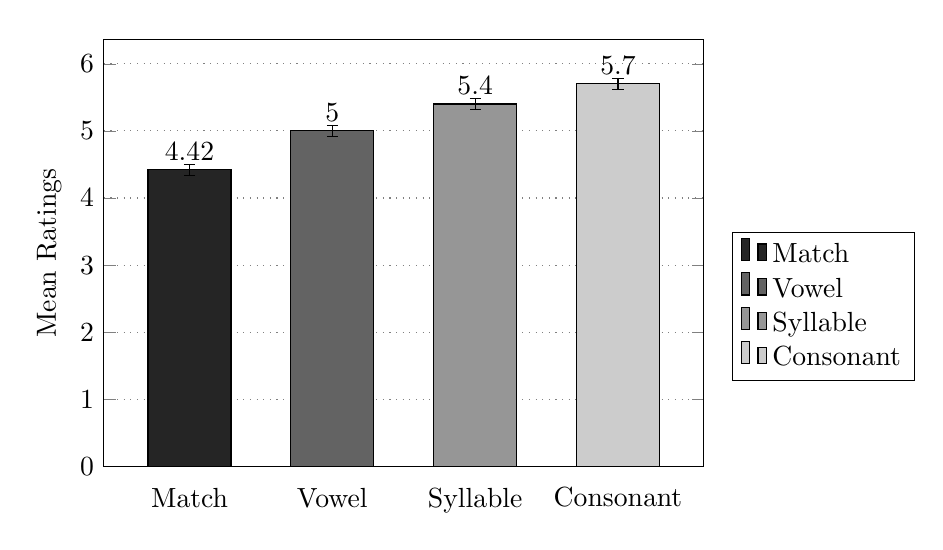
\begin{tikzpicture}
  \begin{axis}[
  ylabel={Mean Ratings},
width=9.2cm,
   height = 7cm,
    ytick distance=1,
        nodes near coords,
      major x tick style = transparent,
    ybar=3*\pgflinewidth,
      bar width=30pt,
      ymajorgrids = true,
      symbolic x coords={Match,Vowel,Syllable,Consonant},
      xtick ={Match,Vowel, Syllable, Consonant},
      scaled y ticks = false,
        legend style={at={(1.2,0.55)},
  anchor=north},
  legend cell align=left,
      enlarge x limits=0.20,
      ymin=0,
       every axis plot/.append style={
          ybar,
          bar shift=0pt,
          fill
        }
    ]
\addplot [fill=mycolor4,error bars/.cd, y dir=both, y explicit,error bar style=black] 
  coordinates {
          (Match, 4.42) += (0,0.08) -= (0,0.08)};
\addplot [fill=mycolor3,error bars/.cd, y dir=both, y explicit,error bar style=black] 
  coordinates {
          (Vowel, 5.00) += (0,0.08) -= (0,0.08)};
\addplot [fill=mycolor2,error bars/.cd, y dir=both, y explicit,error bar style=black] 
  coordinates {
          (Syllable, 5.40) += (0,0.08) -= (0,0.08)};
 \addplot [fill=mycolor1,error bars/.cd, y dir=both, y explicit,error bar style=black] 
  coordinates {
          (Consonant, 5.70) += (0,0.08) -= (0,0.08)};
  \legend{Match,Vowel,Syllable,Consonant}
 \end{axis}
\end{tikzpicture}
\end{center}



\caption{Mean Ratings by Type of Stimuli on the Scale from 1 to 9}
\label{fig:bar2}
\figSpace
\end{figure}

Linear mixed-effects regression models were employed with the \textit{lme4} package in R \citep{Bates_2014} to investigate segmental and syllable influences on foreign accent perception. The regression models were built the same way as the ones used for Experiment 1. Model comparisons were conducted using the Likelihood Ratio Test as described in Chapter 4. The results show that the DTW scores, which represent prosodic differences between L1 and L2 speech samples, and the interactions involving the DTW scores did not contribute significantly to model fit, showing that prosodic information of the stimuli might not be a major contributing factor to accentedness judgment. 

Just as in Experiment 1, types of stimuli were coded using Helmert contrasts. Results show that the contrast between consonant and syllable mismatches did not achieve significant contribution to model fit (χ2=1.60, p=.21), indicating that ratings of stimuli with consonant and syllable mismatches did not differ significantly from each other. The second contrast, which compared vowel mismatches with consonant and syllable mismatches, contributed significantly to model fit (χ2 = 5.15, p < .02), showing that stimuli with consonant and syllable mismatches were rated as being more accented than stimuli with vowel mismatches. The third contrast, which compares the match stimuli with the three types of mismatch stimuli contributed significantly to model fit (χ2 = 19.84, p < .001), showing that stimuli with mismatches were rated as being more foreign-accented than the match stimuli.

These results suggest that all three types of mismatches contributed to perceived foreign-accentedness. Among the three types of mismatches, vowel mismatches were rated to be the least accented. 

\subsection{Ratings across Time}

Just as in Experiment 1, trial number, which represented time, contributed significantly to model fit (β=0.6, χ2 = 69.91, p < .001), while the interactions between trial number and the three contrasts did not contribute significantly to model fit. These results show that ratings of the four types of stimuli increased over time.

Unlike Experiment 1, Experiment 2 included a training phase, containing ten stimuli covering the range of accents included in the experiment. Ratings obtained by Experiment 1 show that the raters were making adjustments during the first few trials. To investigate whether the inclusion of a training phase and the controlling of intelligibility had affected accentedness judgment, a Smoothing Spline ANOVA (SSANOVA) method was implemented with the \textit{gss} package in R \citep{Gu_2013}. The results are shown in Figure \ref{fig:tr2}, where the solid line represents ratings from Experiment 1 and the dotted line represents ratings from Experiment 2. The shaded areas represent 95\% Bayesian confidence intervals. As Figure \ref{fig:tr2} shows, ratings of Experiment 1 experienced a sudden drop during the first 10 to 15 trials and then the ratings went up. However, ratings obtained by Experiment 2 were more consistent. In other words, no adjustment was observed during the testing phase of Experiment 2. Ratings of Experiment 2 were also generally higher than ratings of Experiment 1.

\begin{figure}[!h]
  \figSpace
    \centering
% Created by tikzDevice version 0.12.3 on 2019-11-25 17:34:11
% !TEX encoding = UTF-8 Unicode
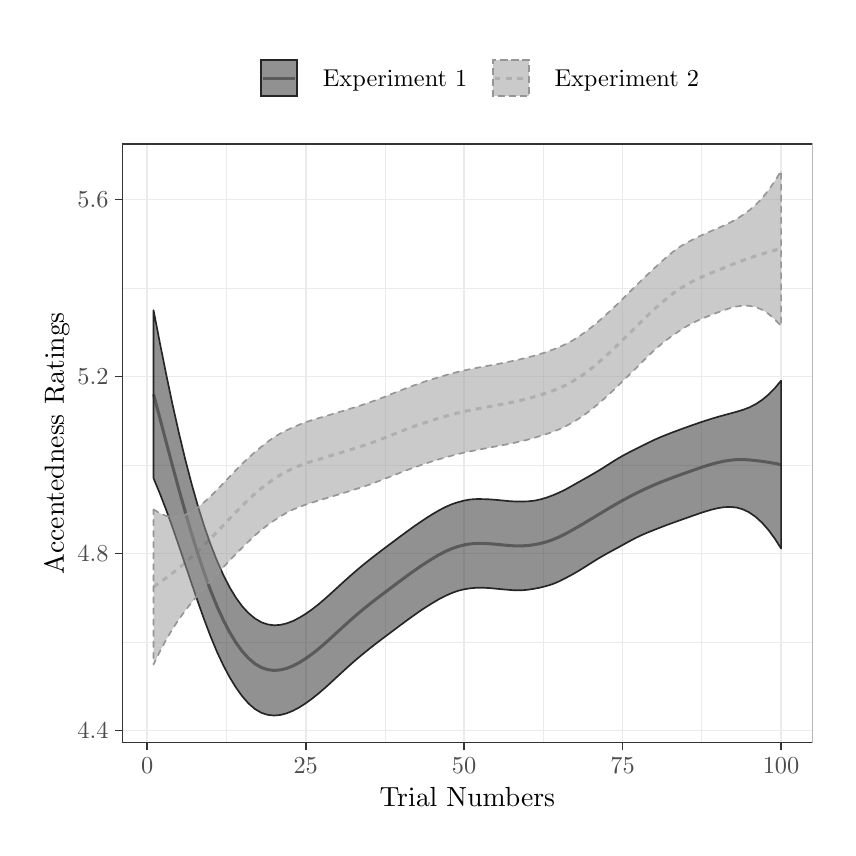
\begin{tikzpicture}[x=1pt,y=1pt]
\definecolor{fillColor}{RGB}{255,255,255}
\path[use as bounding box,fill=fillColor,fill opacity=0.00] (0,0) rectangle (289.08,289.08);
\begin{scope}
\path[clip] (  0.00,  0.00) rectangle (289.08,289.08);
\definecolor{drawColor}{RGB}{255,255,255}
\definecolor{fillColor}{RGB}{255,255,255}

\path[draw=drawColor,line width= 0.6pt,line join=round,line cap=round,fill=fillColor] (  0.00,  0.00) rectangle (289.08,289.08);
\end{scope}
\begin{scope}
\path[clip] ( 34.16, 30.69) rectangle (283.58,247.13);
\definecolor{fillColor}{RGB}{255,255,255}

\path[fill=fillColor] ( 34.16, 30.69) rectangle (283.58,247.13);
\definecolor{drawColor}{gray}{0.92}

\path[draw=drawColor,line width= 0.3pt,line join=round] ( 34.16, 67.10) --
	(283.58, 67.10);

\path[draw=drawColor,line width= 0.3pt,line join=round] ( 34.16,131.06) --
	(283.58,131.06);

\path[draw=drawColor,line width= 0.3pt,line join=round] ( 34.16,195.01) --
	(283.58,195.01);

\path[draw=drawColor,line width= 0.3pt,line join=round] ( 71.83, 30.69) --
	( 71.83,247.13);

\path[draw=drawColor,line width= 0.3pt,line join=round] (129.09, 30.69) --
	(129.09,247.13);

\path[draw=drawColor,line width= 0.3pt,line join=round] (186.35, 30.69) --
	(186.35,247.13);

\path[draw=drawColor,line width= 0.3pt,line join=round] (243.61, 30.69) --
	(243.61,247.13);

\path[draw=drawColor,line width= 0.6pt,line join=round] ( 34.16, 35.13) --
	(283.58, 35.13);

\path[draw=drawColor,line width= 0.6pt,line join=round] ( 34.16, 99.08) --
	(283.58, 99.08);

\path[draw=drawColor,line width= 0.6pt,line join=round] ( 34.16,163.03) --
	(283.58,163.03);

\path[draw=drawColor,line width= 0.6pt,line join=round] ( 34.16,226.99) --
	(283.58,226.99);

\path[draw=drawColor,line width= 0.6pt,line join=round] ( 43.20, 30.69) --
	( 43.20,247.13);

\path[draw=drawColor,line width= 0.6pt,line join=round] (100.46, 30.69) --
	(100.46,247.13);

\path[draw=drawColor,line width= 0.6pt,line join=round] (157.72, 30.69) --
	(157.72,247.13);

\path[draw=drawColor,line width= 0.6pt,line join=round] (214.98, 30.69) --
	(214.98,247.13);

\path[draw=drawColor,line width= 0.6pt,line join=round] (272.24, 30.69) --
	(272.24,247.13);
\definecolor{drawColor}{RGB}{37,37,37}

\path[draw=drawColor,draw opacity=0.50,line width= 1.1pt,line join=round] ( 45.49,156.60) --
	( 47.78,147.92) --
	( 50.07,139.25) --
	( 52.36,130.63) --
	( 54.66,122.19) --
	( 56.95,114.02) --
	( 59.24,106.21) --
	( 61.53, 98.84) --
	( 63.82, 91.98) --
	( 66.11, 85.68) --
	( 68.40, 80.02) --
	( 70.69, 75.00) --
	( 72.98, 70.61) --
	( 75.27, 66.84) --
	( 77.56, 63.69) --
	( 79.85, 61.16) --
	( 82.14, 59.22) --
	( 84.43, 57.88) --
	( 86.72, 57.10) --
	( 89.01, 56.83) --
	( 91.30, 57.00) --
	( 93.59, 57.57) --
	( 95.88, 58.47) --
	( 98.17, 59.67) --
	(100.46, 61.10) --
	(102.75, 62.75) --
	(105.04, 64.56) --
	(107.33, 66.51) --
	(109.62, 68.57) --
	(111.91, 70.69) --
	(114.21, 72.80) --
	(116.50, 74.86) --
	(118.79, 76.86) --
	(121.08, 78.78) --
	(123.37, 80.63) --
	(125.66, 82.42) --
	(127.95, 84.17) --
	(130.24, 85.88) --
	(132.53, 87.60) --
	(134.82, 89.32) --
	(137.11, 91.01) --
	(139.40, 92.66) --
	(141.69, 94.26) --
	(143.98, 95.78) --
	(146.27, 97.23) --
	(148.56, 98.57) --
	(150.85, 99.77) --
	(153.14,100.78) --
	(155.43,101.58) --
	(157.72,102.17) --
	(160.01,102.55) --
	(162.30,102.72) --
	(164.59,102.72) --
	(166.88,102.60) --
	(169.17,102.41) --
	(171.47,102.19) --
	(173.76,101.97) --
	(176.05,101.82) --
	(178.34,101.80) --
	(180.63,101.94) --
	(182.92,102.23) --
	(185.21,102.68) --
	(187.50,103.30) --
	(189.79,104.09) --
	(192.08,105.06) --
	(194.37,106.20) --
	(196.66,107.45) --
	(198.95,108.76) --
	(201.24,110.11) --
	(203.53,111.48) --
	(205.82,112.87) --
	(208.11,114.25) --
	(210.40,115.62) --
	(212.69,116.96) --
	(214.98,118.25) --
	(217.27,119.49) --
	(219.56,120.67) --
	(221.85,121.80) --
	(224.14,122.86) --
	(226.43,123.88) --
	(228.73,124.83) --
	(231.02,125.73) --
	(233.31,126.59) --
	(235.60,127.42) --
	(237.89,128.24) --
	(240.18,129.05) --
	(242.47,129.85) --
	(244.76,130.61) --
	(247.05,131.32) --
	(249.34,131.93) --
	(251.63,132.43) --
	(253.92,132.79) --
	(256.21,132.99) --
	(258.50,133.01) --
	(260.79,132.88) --
	(263.08,132.66) --
	(265.37,132.37) --
	(267.66,132.03) --
	(269.95,131.63) --
	(272.24,131.19);
\definecolor{drawColor}{RGB}{150,150,150}

\path[draw=drawColor,draw opacity=0.50,line width= 1.1pt,dash pattern=on 2pt off 2pt ,line join=round] ( 45.49, 87.00) --
	( 47.78, 88.64) --
	( 50.07, 90.32) --
	( 52.36, 92.03) --
	( 54.66, 93.84) --
	( 56.95, 95.76) --
	( 59.24, 97.78) --
	( 61.53, 99.92) --
	( 63.82,102.15) --
	( 66.11,104.47) --
	( 68.40,106.85) --
	( 70.69,109.26) --
	( 72.98,111.68) --
	( 75.27,114.06) --
	( 77.56,116.37) --
	( 79.85,118.58) --
	( 82.14,120.67) --
	( 84.43,122.62) --
	( 86.72,124.41) --
	( 89.01,126.03) --
	( 91.30,127.45) --
	( 93.59,128.71) --
	( 95.88,129.81) --
	( 98.17,130.77) --
	(100.46,131.62) --
	(102.75,132.38) --
	(105.04,133.07) --
	(107.33,133.75) --
	(109.62,134.43) --
	(111.91,135.12) --
	(114.21,135.82) --
	(116.50,136.53) --
	(118.79,137.25) --
	(121.08,137.99) --
	(123.37,138.77) --
	(125.66,139.60) --
	(127.95,140.47) --
	(130.24,141.37) --
	(132.53,142.28) --
	(134.82,143.19) --
	(137.11,144.07) --
	(139.40,144.92) --
	(141.69,145.72) --
	(143.98,146.49) --
	(146.27,147.23) --
	(148.56,147.94) --
	(150.85,148.61) --
	(153.14,149.24) --
	(155.43,149.83) --
	(157.72,150.37) --
	(160.01,150.86) --
	(162.30,151.31) --
	(164.59,151.74) --
	(166.88,152.17) --
	(169.17,152.59) --
	(171.47,153.02) --
	(173.76,153.48) --
	(176.05,153.95) --
	(178.34,154.47) --
	(180.63,155.04) --
	(182.92,155.67) --
	(185.21,156.34) --
	(187.50,157.08) --
	(189.79,157.90) --
	(192.08,158.81) --
	(194.37,159.87) --
	(196.66,161.10) --
	(198.95,162.50) --
	(201.24,164.07) --
	(203.53,165.81) --
	(205.82,167.69) --
	(208.11,169.69) --
	(210.40,171.78) --
	(212.69,173.94) --
	(214.98,176.16) --
	(217.27,178.42) --
	(219.56,180.70) --
	(221.85,182.96) --
	(224.14,185.18) --
	(226.43,187.34) --
	(228.73,189.39) --
	(231.02,191.33) --
	(233.31,193.11) --
	(235.60,194.72) --
	(237.89,196.13) --
	(240.18,197.37) --
	(242.47,198.48) --
	(244.76,199.50) --
	(247.05,200.46) --
	(249.34,201.39) --
	(251.63,202.31) --
	(253.92,203.23) --
	(256.21,204.15) --
	(258.50,205.02) --
	(260.79,205.84) --
	(263.08,206.59) --
	(265.37,207.31) --
	(267.66,207.98) --
	(269.95,208.64) --
	(272.24,209.28);
\definecolor{drawColor}{RGB}{37,37,37}
\definecolor{fillColor}{RGB}{37,37,37}

\path[draw=drawColor,line width= 0.6pt,line join=round,line cap=round,fill=fillColor,fill opacity=0.50] ( 45.49,186.96) --
	( 47.78,175.12) --
	( 50.07,163.72) --
	( 52.36,152.84) --
	( 54.66,142.58) --
	( 56.95,133.04) --
	( 59.24,124.23) --
	( 61.53,116.17) --
	( 63.82,108.85) --
	( 66.11,102.31) --
	( 68.40, 96.50) --
	( 70.69, 91.34) --
	( 72.98, 86.86) --
	( 75.27, 83.07) --
	( 77.56, 79.95) --
	( 79.85, 77.48) --
	( 82.14, 75.59) --
	( 84.43, 74.23) --
	( 86.72, 73.44) --
	( 89.01, 73.13) --
	( 91.30, 73.28) --
	( 93.59, 73.82) --
	( 95.88, 74.69) --
	( 98.17, 75.86) --
	(100.46, 77.27) --
	(102.75, 78.88) --
	(105.04, 80.67) --
	(107.33, 82.62) --
	(109.62, 84.67) --
	(111.91, 86.77) --
	(114.21, 88.88) --
	(116.50, 90.92) --
	(118.79, 92.92) --
	(121.08, 94.85) --
	(123.37, 96.69) --
	(125.66, 98.47) --
	(127.95,100.23) --
	(130.24,101.94) --
	(132.53,103.65) --
	(134.82,105.37) --
	(137.11,107.06) --
	(139.40,108.72) --
	(141.69,110.30) --
	(143.98,111.83) --
	(146.27,113.28) --
	(148.56,114.62) --
	(150.85,115.83) --
	(153.14,116.82) --
	(155.43,117.59) --
	(157.72,118.20) --
	(160.01,118.61) --
	(162.30,118.75) --
	(164.59,118.73) --
	(166.88,118.64) --
	(169.17,118.46) --
	(171.47,118.24) --
	(173.76,118.01) --
	(176.05,117.87) --
	(178.34,117.84) --
	(180.63,117.91) --
	(182.92,118.14) --
	(185.21,118.60) --
	(187.50,119.27) --
	(189.79,120.12) --
	(192.08,121.10) --
	(194.37,122.21) --
	(196.66,123.49) --
	(198.95,124.80) --
	(201.24,126.08) --
	(203.53,127.37) --
	(205.82,128.71) --
	(208.11,130.13) --
	(210.40,131.59) --
	(212.69,133.04) --
	(214.98,134.38) --
	(217.27,135.59) --
	(219.56,136.73) --
	(221.85,137.88) --
	(224.14,139.03) --
	(226.43,140.14) --
	(228.73,141.14) --
	(231.02,142.07) --
	(233.31,142.96) --
	(235.60,143.80) --
	(237.89,144.64) --
	(240.18,145.45) --
	(242.47,146.24) --
	(244.76,147.01) --
	(247.05,147.74) --
	(249.34,148.42) --
	(251.63,149.06) --
	(253.92,149.67) --
	(256.21,150.30) --
	(258.50,151.00) --
	(260.79,151.87) --
	(263.08,153.04) --
	(265.37,154.56) --
	(267.66,156.46) --
	(269.95,158.78) --
	(272.24,161.52) --
	(272.24,100.87) --
	(269.95,104.48) --
	(267.66,107.59) --
	(265.37,110.19) --
	(263.08,112.28) --
	(260.79,113.89) --
	(258.50,115.01) --
	(256.21,115.67) --
	(253.92,115.91) --
	(251.63,115.81) --
	(249.34,115.45) --
	(247.05,114.89) --
	(244.76,114.21) --
	(242.47,113.45) --
	(240.18,112.66) --
	(237.89,111.85) --
	(235.60,111.05) --
	(233.31,110.22) --
	(231.02,109.39) --
	(228.73,108.52) --
	(226.43,107.61) --
	(224.14,106.70) --
	(221.85,105.72) --
	(219.56,104.62) --
	(217.27,103.40) --
	(214.98,102.13) --
	(212.69,100.88) --
	(210.40, 99.65) --
	(208.11, 98.37) --
	(205.82, 97.02) --
	(203.53, 95.59) --
	(201.24, 94.13) --
	(198.95, 92.72) --
	(196.66, 91.41) --
	(194.37, 90.18) --
	(192.08, 89.02) --
	(189.79, 88.06) --
	(187.50, 87.33) --
	(185.21, 86.76) --
	(182.92, 86.31) --
	(180.63, 85.96) --
	(178.34, 85.77) --
	(176.05, 85.77) --
	(173.76, 85.94) --
	(171.47, 86.14) --
	(169.17, 86.36) --
	(166.88, 86.57) --
	(164.59, 86.71) --
	(162.30, 86.69) --
	(160.01, 86.50) --
	(157.72, 86.14) --
	(155.43, 85.57) --
	(153.14, 84.74) --
	(150.85, 83.72) --
	(148.56, 82.53) --
	(146.27, 81.17) --
	(143.98, 79.74) --
	(141.69, 78.22) --
	(139.40, 76.61) --
	(137.11, 74.96) --
	(134.82, 73.26) --
	(132.53, 71.54) --
	(130.24, 69.83) --
	(127.95, 68.11) --
	(125.66, 66.37) --
	(123.37, 64.57) --
	(121.08, 62.72) --
	(118.79, 60.81) --
	(116.50, 58.81) --
	(114.21, 56.72) --
	(111.91, 54.61) --
	(109.62, 52.48) --
	(107.33, 50.40) --
	(105.04, 48.44) --
	(102.75, 46.61) --
	(100.46, 44.94) --
	( 98.17, 43.47) --
	( 95.88, 42.26) --
	( 93.59, 41.32) --
	( 91.30, 40.72) --
	( 89.01, 40.52) --
	( 86.72, 40.77) --
	( 84.43, 41.52) --
	( 82.14, 42.85) --
	( 79.85, 44.83) --
	( 77.56, 47.43) --
	( 75.27, 50.62) --
	( 72.98, 54.35) --
	( 70.69, 58.65) --
	( 68.40, 63.55) --
	( 66.11, 69.06) --
	( 63.82, 75.10) --
	( 61.53, 81.51) --
	( 59.24, 88.20) --
	( 56.95, 95.00) --
	( 54.66,101.79) --
	( 52.36,108.42) --
	( 50.07,114.78) --
	( 47.78,120.71) --
	( 45.49,126.25) --
	cycle;
\definecolor{drawColor}{gray}{0.59}
\definecolor{fillColor}{RGB}{150,150,150}

\path[draw=drawColor,line width= 0.6pt,dash pattern=on 2pt off 2pt ,line join=round,line cap=round,fill=fillColor,fill opacity=0.50] ( 45.49,115.03) --
	( 47.78,113.59) --
	( 50.07,112.65) --
	( 52.36,112.24) --
	( 54.66,112.37) --
	( 56.95,113.04) --
	( 59.24,114.20) --
	( 61.53,115.76) --
	( 63.82,117.65) --
	( 66.11,119.76) --
	( 68.40,122.05) --
	( 70.69,124.44) --
	( 72.98,126.82) --
	( 75.27,129.20) --
	( 77.56,131.53) --
	( 79.85,133.70) --
	( 82.14,135.72) --
	( 84.43,137.64) --
	( 86.72,139.45) --
	( 89.01,141.09) --
	( 91.30,142.45) --
	( 93.59,143.61) --
	( 95.88,144.66) --
	( 98.17,145.64) --
	(100.46,146.53) --
	(102.75,147.28) --
	(105.04,147.96) --
	(107.33,148.62) --
	(109.62,149.29) --
	(111.91,149.99) --
	(114.21,150.67) --
	(116.50,151.39) --
	(118.79,152.08) --
	(121.08,152.82) --
	(123.37,153.62) --
	(125.66,154.42) --
	(127.95,155.27) --
	(130.24,156.20) --
	(132.53,157.13) --
	(134.82,158.03) --
	(137.11,158.93) --
	(139.40,159.76) --
	(141.69,160.57) --
	(143.98,161.35) --
	(146.27,162.07) --
	(148.56,162.78) --
	(150.85,163.46) --
	(153.14,164.09) --
	(155.43,164.68) --
	(157.72,165.22) --
	(160.01,165.71) --
	(162.30,166.15) --
	(164.59,166.59) --
	(166.88,167.00) --
	(169.17,167.40) --
	(171.47,167.86) --
	(173.76,168.33) --
	(176.05,168.80) --
	(178.34,169.32) --
	(180.63,169.90) --
	(182.92,170.50) --
	(185.21,171.16) --
	(187.50,171.92) --
	(189.79,172.75) --
	(192.08,173.66) --
	(194.37,174.71) --
	(196.66,175.91) --
	(198.95,177.33) --
	(201.24,178.92) --
	(203.53,180.65) --
	(205.82,182.54) --
	(208.11,184.55) --
	(210.40,186.65) --
	(212.69,188.80) --
	(214.98,191.02) --
	(217.27,193.33) --
	(219.56,195.62) --
	(221.85,197.83) --
	(224.14,200.00) --
	(226.43,202.14) --
	(228.73,204.26) --
	(231.02,206.30) --
	(233.31,208.20) --
	(235.60,209.85) --
	(237.89,211.22) --
	(240.18,212.42) --
	(242.47,213.56) --
	(244.76,214.63) --
	(247.05,215.63) --
	(249.34,216.60) --
	(251.63,217.61) --
	(253.92,218.71) --
	(256.21,219.96) --
	(258.50,221.43) --
	(260.79,223.11) --
	(263.08,225.07) --
	(265.37,227.44) --
	(267.66,230.28) --
	(269.95,233.58) --
	(272.24,237.29) --
	(272.24,181.28) --
	(269.95,183.70) --
	(267.66,185.69) --
	(265.37,187.17) --
	(263.08,188.11) --
	(260.79,188.56) --
	(258.50,188.62) --
	(256.21,188.34) --
	(253.92,187.76) --
	(251.63,187.01) --
	(249.34,186.18) --
	(247.05,185.29) --
	(244.76,184.36) --
	(242.47,183.40) --
	(240.18,182.32) --
	(237.89,181.04) --
	(235.60,179.59) --
	(233.31,178.03) --
	(231.02,176.36) --
	(228.73,174.53) --
	(226.43,172.53) --
	(224.14,170.36) --
	(221.85,168.08) --
	(219.56,165.77) --
	(217.27,163.51) --
	(214.98,161.30) --
	(212.69,159.08) --
	(210.40,156.90) --
	(208.11,154.82) --
	(205.82,152.85) --
	(203.53,150.97) --
	(201.24,149.22) --
	(198.95,147.67) --
	(196.66,146.29) --
	(194.37,145.04) --
	(192.08,143.96) --
	(189.79,143.05) --
	(187.50,142.25) --
	(185.21,141.53) --
	(182.92,140.83) --
	(180.63,140.19) --
	(178.34,139.63) --
	(176.05,139.10) --
	(173.76,138.62) --
	(171.47,138.19) --
	(169.17,137.78) --
	(166.88,137.33) --
	(164.59,136.89) --
	(162.30,136.47) --
	(160.01,136.01) --
	(157.72,135.52) --
	(155.43,134.99) --
	(153.14,134.39) --
	(150.85,133.76) --
	(148.56,133.10) --
	(146.27,132.39) --
	(143.98,131.64) --
	(141.69,130.87) --
	(139.40,130.07) --
	(137.11,129.22) --
	(134.82,128.35) --
	(132.53,127.43) --
	(130.24,126.54) --
	(127.95,125.66) --
	(125.66,124.77) --
	(123.37,123.92) --
	(121.08,123.16) --
	(118.79,122.41) --
	(116.50,121.67) --
	(114.21,120.97) --
	(111.91,120.26) --
	(109.62,119.58) --
	(107.33,118.88) --
	(105.04,118.18) --
	(102.75,117.47) --
	(100.46,116.71) --
	( 98.17,115.90) --
	( 95.88,114.95) --
	( 93.59,113.81) --
	( 91.30,112.46) --
	( 89.01,110.97) --
	( 86.72,109.36) --
	( 84.43,107.59) --
	( 82.14,105.61) --
	( 79.85,103.45) --
	( 77.56,101.20) --
	( 75.27, 98.92) --
	( 72.98, 96.53) --
	( 70.69, 94.08) --
	( 68.40, 91.65) --
	( 66.11, 89.17) --
	( 63.82, 86.64) --
	( 61.53, 84.07) --
	( 59.24, 81.36) --
	( 56.95, 78.47) --
	( 54.66, 75.31) --
	( 52.36, 71.83) --
	( 50.07, 67.98) --
	( 47.78, 63.70) --
	( 45.49, 58.97) --
	cycle;
\definecolor{drawColor}{gray}{0.20}

\path[draw=drawColor,line width= 0.6pt,line join=round,line cap=round] ( 34.16, 30.69) rectangle (283.58,247.13);
\end{scope}
\begin{scope}
\path[clip] (  0.00,  0.00) rectangle (289.08,289.08);
\definecolor{drawColor}{gray}{0.30}

\node[text=drawColor,anchor=base east,inner sep=0pt, outer sep=0pt, scale=  0.88] at ( 29.21, 32.10) {4.4};

\node[text=drawColor,anchor=base east,inner sep=0pt, outer sep=0pt, scale=  0.88] at ( 29.21, 96.05) {4.8};

\node[text=drawColor,anchor=base east,inner sep=0pt, outer sep=0pt, scale=  0.88] at ( 29.21,160.00) {5.2};

\node[text=drawColor,anchor=base east,inner sep=0pt, outer sep=0pt, scale=  0.88] at ( 29.21,223.96) {5.6};
\end{scope}
\begin{scope}
\path[clip] (  0.00,  0.00) rectangle (289.08,289.08);
\definecolor{drawColor}{gray}{0.20}

\path[draw=drawColor,line width= 0.6pt,line join=round] ( 31.41, 35.13) --
	( 34.16, 35.13);

\path[draw=drawColor,line width= 0.6pt,line join=round] ( 31.41, 99.08) --
	( 34.16, 99.08);

\path[draw=drawColor,line width= 0.6pt,line join=round] ( 31.41,163.03) --
	( 34.16,163.03);

\path[draw=drawColor,line width= 0.6pt,line join=round] ( 31.41,226.99) --
	( 34.16,226.99);
\end{scope}
\begin{scope}
\path[clip] (  0.00,  0.00) rectangle (289.08,289.08);
\definecolor{drawColor}{gray}{0.20}

\path[draw=drawColor,line width= 0.6pt,line join=round] ( 43.20, 27.94) --
	( 43.20, 30.69);

\path[draw=drawColor,line width= 0.6pt,line join=round] (100.46, 27.94) --
	(100.46, 30.69);

\path[draw=drawColor,line width= 0.6pt,line join=round] (157.72, 27.94) --
	(157.72, 30.69);

\path[draw=drawColor,line width= 0.6pt,line join=round] (214.98, 27.94) --
	(214.98, 30.69);

\path[draw=drawColor,line width= 0.6pt,line join=round] (272.24, 27.94) --
	(272.24, 30.69);
\end{scope}
\begin{scope}
\path[clip] (  0.00,  0.00) rectangle (289.08,289.08);
\definecolor{drawColor}{gray}{0.30}

\node[text=drawColor,anchor=base,inner sep=0pt, outer sep=0pt, scale=  0.88] at ( 43.20, 19.68) {0};

\node[text=drawColor,anchor=base,inner sep=0pt, outer sep=0pt, scale=  0.88] at (100.46, 19.68) {25};

\node[text=drawColor,anchor=base,inner sep=0pt, outer sep=0pt, scale=  0.88] at (157.72, 19.68) {50};

\node[text=drawColor,anchor=base,inner sep=0pt, outer sep=0pt, scale=  0.88] at (214.98, 19.68) {75};

\node[text=drawColor,anchor=base,inner sep=0pt, outer sep=0pt, scale=  0.88] at (272.24, 19.68) {100};
\end{scope}
\begin{scope}
\path[clip] (  0.00,  0.00) rectangle (289.08,289.08);
\definecolor{drawColor}{RGB}{0,0,0}

\node[text=drawColor,anchor=base,inner sep=0pt, outer sep=0pt, scale=  1.00] at (158.87,  7.64) {Trial Numbers};
\end{scope}
\begin{scope}
\path[clip] (  0.00,  0.00) rectangle (289.08,289.08);
\definecolor{drawColor}{RGB}{0,0,0}

\node[text=drawColor,rotate= 90.00,anchor=base,inner sep=0pt, outer sep=0pt, scale=  1.00] at ( 13.08,138.91) {Accentedness Ratings};
\end{scope}
\begin{scope}
\path[clip] (  0.00,  0.00) rectangle (289.08,289.08);
\definecolor{fillColor}{RGB}{255,255,255}

\path[fill=fillColor] ( 69.64,258.13) rectangle (248.09,283.58);
\end{scope}
\begin{scope}
\path[clip] (  0.00,  0.00) rectangle (289.08,289.08);
\definecolor{fillColor}{RGB}{255,255,255}

\path[fill=fillColor] ( 83.68,263.63) rectangle ( 98.13,278.08);
\end{scope}
\begin{scope}
\path[clip] (  0.00,  0.00) rectangle (289.08,289.08);
\definecolor{drawColor}{RGB}{37,37,37}

\path[draw=drawColor,draw opacity=0.50,line width= 1.1pt,line join=round] ( 85.12,270.85) -- ( 96.69,270.85);
\end{scope}
\begin{scope}
\path[clip] (  0.00,  0.00) rectangle (289.08,289.08);
\definecolor{drawColor}{RGB}{37,37,37}
\definecolor{fillColor}{RGB}{37,37,37}

\path[draw=drawColor,line width= 0.6pt,line cap=rect,fill=fillColor,fill opacity=0.50] ( 84.39,264.34) rectangle ( 97.42,277.37);
\end{scope}
\begin{scope}
\path[clip] (  0.00,  0.00) rectangle (289.08,289.08);
\definecolor{fillColor}{RGB}{255,255,255}

\path[fill=fillColor] (167.40,263.63) rectangle (181.86,278.08);
\end{scope}
\begin{scope}
\path[clip] (  0.00,  0.00) rectangle (289.08,289.08);
\definecolor{drawColor}{RGB}{150,150,150}

\path[draw=drawColor,draw opacity=0.50,line width= 1.1pt,dash pattern=on 2pt off 2pt ,line join=round] (168.85,270.85) -- (180.41,270.85);
\end{scope}
\begin{scope}
\path[clip] (  0.00,  0.00) rectangle (289.08,289.08);
\definecolor{drawColor}{gray}{0.59}
\definecolor{fillColor}{RGB}{150,150,150}

\path[draw=drawColor,line width= 0.6pt,dash pattern=on 2pt off 2pt ,line cap=rect,fill=fillColor,fill opacity=0.50] (168.12,264.34) rectangle (181.15,277.37);
\end{scope}
\begin{scope}
\path[clip] (  0.00,  0.00) rectangle (289.08,289.08);
\definecolor{drawColor}{RGB}{0,0,0}

\node[text=drawColor,anchor=base west,inner sep=0pt, outer sep=0pt, scale=  0.88] at (106.67,267.82) {Experiment 1};
\end{scope}
\begin{scope}
\path[clip] (  0.00,  0.00) rectangle (289.08,289.08);
\definecolor{drawColor}{RGB}{0,0,0}

\node[text=drawColor,anchor=base west,inner sep=0pt, outer sep=0pt, scale=  0.88] at (190.39,267.82) {Experiment 2};
\end{scope}
\end{tikzpicture}

    \caption{Ratings across Time (Experiment 1 and Experiment 2)}
    \label{fig:tr2}
  \figSpace
\end{figure}

The ten training phase stimuli were also used in the testing phase.  It is possible that the raters' judgments on these ten stimuli during the testing phase are different from their judgments on other stimuli, simply because the ten stimuli were heard during the training phase. Linear mixed-effects model was run to investigate whether ratings on the ten stimuli during the testing phase are different from ratings on the remaining 90 stimuli. The ratings were the dependent variable.The times a stimulus was heard (once vs. twice), the four types of stimuli, trial number and the interactions between these factors were included as fixed effects. The raters and the stimuli were entered as two random effects. The results show that the times a stimulus was heard did not contribute significantly to model fit (χ2 = 0.01, p = .93). Therefore, ratings of the ten stimuli during the testing phase might not have been affected by the fact that the ten stimuli were included the training phase.


\subsection{Individual Mismatches}

The analysis above focuses on broad categories such as consonant, vowel, and syllable mismatches. However, there were 11 types of consonant mismatches, five types of vowel mismatches and two types of syllable mismatches involved in the experiment. Although consonant mismatches appeared in general to be more accented than the other two types of mismatches, it might be too hasty to draw the conclusion that all consonant mismatches are more accented than the other two types. This section presents a more detailed analysis, which focuses on individual mismatches within a given phonological context. The following section first discusses the statistical methods using one phonological context as an example. Since statistical methods used for the other four phonological contexts are the same as methods used for the first context, the details for these four contexts are omitted. 

\subsubsection{Context 1: “\textit{Ask her}”}

For the context “\textit{ask her},” syllable mismatches such as consonant deletion (i.e., [æsk]$\rightarrow$[æs]) and vowel epenthesis (i.e., [æsk]$\rightarrow$[æskə]) received the highest ratings (i.e., most accented), while vowel mismatches received relatively lower ratings. Figure \ref{fig:ah2} demonstrates the mean ratings of the seven individual mismatches and the match stimuli, where the error bars represent 95\% confidence intervals. 

\begin{figure}[!h]
  \figSpace
\centering

\begin{tikzpicture}
  \begin{axis}[
  title={Mean Accentedness Ratings},
     % xbar,
   ytick={1,2,3,4,5,6,7,8},
     y=1cm,
  bar width=0.7 cm,
  xmin=0,
  xmax=7.1,
    axis y line*=left,
   axis x line=bottom,
    tickwidth         = 1pt,
    enlarge y limits  = 0.1,
    enlarge x limits  = 0.02,
  legend style={at={(1.2,0.55)},
  anchor=north},
  legend cell align=left,
      yticklabels from table={figures/sup/data_askher.txt}{label},
      xtick distance=2,
      every axis plot/.append style={
          xbar,
          bar shift=0pt,
          fill
        }
    ]
\addplot [fill=red,color=mycolor3,select coords between index={0}{0}] table  [x=x,y=y] {figures/sup/data_askher.txt};
\addplot [fill=red,color=mycolor1,select coords between index={1}{1}] table  [x=x,y=y] {figures/sup/data_askher.txt};
\addplot [fill=blue,color=mycolor3,select coords between index={2}{4}] table [x=x, y=y] {figures/sup/data_askher.txt};
\addplot [fill=blue,color=mycolor4,select coords between index={5}{5}] table [x=x, y=y] {figures/sup/data_askher.txt};
\addplot [fill=blue,color=mycolor2,select coords between index={6}{7}] table [x=x, y=y] {figures/sup/data_askher.txt};

 \addplot [color=black, only marks, mark=o]
 plot [error bars/.cd, x dir = both, x explicit]
 table[x =x, y =y, x error =err]{figures/sup/data_askher.txt};
 \end{axis}
\node[] at (7.5,7.7) {6.96};
\node[] at (7.08,6.7) {6.54};
\node[] at (6.45,5.7) {6.00};
\node[] at (6.4,4.7) {5.77};
\node[] at (6.14,3.7) {5.49};
\node[] at (5.65,2.7) {5.10};
\node[] at (5.31,1.7) {4.85};
\node[] at (5.15,0.7) {4.45};
\end{tikzpicture}
\caption{Mean Accentedness Ratings of Stimuli in “\textit{Ask her}”}
\label{fig:ah2}
\figSpace
\end{figure}

Ratings in Figure \ref{fig:ah2} showed that consonant deletion (i.e., [æsk]$\rightarrow$[as]) and vowel epenthesis (i.e., [æsk]$\rightarrow$[æskə]) received the highest ratings, while the match stimuli and vowel lowering (i.e., [æ]$\rightarrow$[æ̞]) received the lowest ratings. Vowel backing (i.e., [æ]$\rightarrow$[ɑ]) and vowel raisings (i.e., [æ]$\rightarrow$[æ̝]) received relatively higher ratings than vowel lowering. The mean rating for consonant change (i.e., [ɹ]$\rightarrow$[r]) was relatively lower than the two syllable mismatches, but higher than all the vowel mismatches. To evaluate whether the rating differences observed in Figure \ref{fig:ah2} are statistically significant, mixed-effects linear regression models were constructed to investigate the effect of individual mismatches on accentedness.

Ratings were the dependent variable. The eight types of stimuli and trial number were entered as fixed effects. Raters were entered as a random effect with types of stimuli as the random slope. Stimuli were entered as another random effect. DTW scores were not included in the model since analysis in the previous section found no evidence of the effect of DTW on accentedness ratings. Model comparisons using likelihood ratio tests revealed that type of stimuli contributed significantly to model fit (χ2 = 26.42, p < .001), showing that the eight types of stimuli were indeed rated differently. Trial number was another significant contributing factor to model fit (β=0.03, χ2 = 10.20, p < .001), showing that the same stimulus would be considered more accented if it occurred late in the experiment. The interaction between the type of stimuli and trial numbers did not contribute significantly to model fit (χ2 = 6.28, p =.51), showing that rating differences between the four types of stimuli were consistent overt ime. 

To further investigate pairwise rating differences between the eight type of stimuli, Helmert-contrast-coding was implemented to create seven contrasts (Table \ref{table:contr2}), which were entered into another mixed-effects model as seven fixed effects. Trial number and the interactions between trial number and the seven contrasts were also entered as fixed effects. Raters and stimuli were used as random effects. 

\begin{table}[!h]
  \figSpace
\centering
  \caption{Stimuli Contrasts}
  \label{table:contr2}%
\begin{tabular}{lrrrrrrr}
	\toprule
  Levels & Contrast1 & Contrast2 & Contrast3 & Contrast4 & Contrast5 & Contrast6 & Contrast7 \\
    \midrule
    æ$\rightarrow$æ̞    & -0.5  & -0.333 & -0.25 & -0.2  & -0.167 & -0.143 & -0.125 \\
    Match     & 0.5   & -0.333 & -0.25 & -0.2  & -0.167 & -0.143 & -0.125 \\
    æ$\rightarrow$a     & 0     & 0.667 & -0.25 & -0.2  & -0.167 & -0.143 & -0.125 \\
    æ$\rightarrow$æ̝     & 0     & 0     & 0.75  & -0.2  & -0.167 & -0.143 & -0.125 \\
    æ$\rightarrow$ɑ     & 0     & 0     & 0     & 0.8   & -0.167 & -0.143 & -0.125 \\
    æsk$\rightarrow$æs     & 0     & 0     & 0     & 0     & 0.833 & -0.143 & -0.125 \\
    ɹ$\rightarrow$r     & 0     & 0     & 0     & 0     & 0     & 0.857 & -0.125 \\
    æsk$\rightarrow$æskə    & 0     & 0     & 0     & 0     & 0     & 0     & 0.875 \\
    \bottomrule     
\end{tabular}
  \figSpace
\end{table}

Model comparisons were achieved using likelihood ratio tests as described previously in Chapter 4. The results show that the fifth, the sixth and the seventh contrasts contributed significantly to model fit, while the other four contrasts did not contribute significantly to model fit. These results show that syllable mismatches (i.e., [æsk]$\rightarrow$[æskə], [æsk]$\rightarrow$[æs]) and /ɹ/-trilling in “her” were more accented than other types of stimuli. Contrasts were reconstructed in several different ways to allow pairwise comparisons of different types of stimuli. 

The results are listed in Table \ref{table:ah2} where the “$\gg$” symbol indicates significant differences. The types of stimuli on the left side of “$\gg$” were judged as being more accented than types of stimuli on the right side of “$\gg$”. The types of stimuli on the same side of the “$\gg$” did not differ significantly from one another.

\begin{table}[!h]
  \figSpace
  \centering
  \caption{Accentedness Ratings for “\textit{Ask her}” }
  \label{table:ah2}%
    \begin{tabular}{lclcl}
    \toprule
 	æsk$\rightarrow$æs & $\gg$ & æsk$\rightarrow$æskə &$\gg$& æ$\rightarrow$a; Match; æ$\rightarrow$æ̞;\\
 	æsk$\rightarrow$æs & $\gg$ & æ$\rightarrow$æ̝ &$\gg$& Match; æ$\rightarrow$æ̞\\
 	\multicolumn{5}{l}{æ$\rightarrow$æ̝; æ$\rightarrow$ɑ; ɹ$\rightarrow$r; æ$\rightarrow$a (no significant difference)}\\
    \bottomrule
    \end{tabular}%
      \figSpace
\end{table}%

Table \ref{table:ah2} lists three rankings. The first row shows that ratings of [æsk]$\rightarrow$[æs] were significantly higher than ratings of [æsk]$\rightarrow$[æskə], which were significantly higher than ratings of [æ]$\rightarrow$[a], the match stimuli or [æ]-[æ̞]. 

 [æ]$\rightarrow$[ɑ] and [ɹ]$\rightarrow$[r] are missing from the first row, because ratings of these two stimuli were not significantly lower than ratings of [æsk]$\rightarrow$[æskə] or significantly higher than ratings of [æ]$\rightarrow$[a]. Therefore, [æ]$\rightarrow$[ɑ] and [ɹ]$\rightarrow$[r] could not be placed at any side of the “$\gg$”s. [æ]$\rightarrow$[æ̝] was also missing from the first row, because its ratings were not significantly higher than [æ]$\rightarrow$[a], but significantly higher than ratings of the match stimuli or [æ]$\rightarrow$[æ̞]. 

Two more rankings were therefore created to specify accentedness rankings regarding  [æ]$\rightarrow$[ɑ], [ɹ]$\rightarrow$[r] and [æ]$\rightarrow$[æ̞]. The second row lists the second ranking that shows that ratings of these three stimuli were significantly lower than ratings of [æsk]$\rightarrow$[æs], but significantly higher than ratings of the match stimuli or [æ]$\rightarrow$[æ̞]. The third row lists the third ranking, showing that ratings of [æ]$\rightarrow$[æ̝] were significantly lower than [æsk]$\rightarrow$[æskə]. The fourth row shows that ratings of [æ]$\rightarrow$[æ̝], [æ]$\rightarrow$[ɑ], [ɹ]$\rightarrow$[r], [æ]$\rightarrow$[a] did not differ significantly from one another. 

The rankings above show that [æsk]$\rightarrow$[æs] and [æsk]$\rightarrow$[æskə] are the two types of mismatches that were judged as being the most accented. The deletion of /k/ in “\textit{ask}” was considered more accented than vowel epenthesis. Four mismatches of “\textit{ask}” were included in the experiment, namely [ask, æsk, æ̝sk, æ̞sk, ɑsk]. The diacritic marks of [æ̝] and [æ̞] indicate that these two pronunciations are sub-phonemic variations of /æ/. In Experiment 1, ratings of the various vowel mismatches in the context of "ask her" did not show any significant difference. In Experiment 2, vowel raising (i.e., [æ̝]) was rated as more accented than vowel lowering (i.e., [æ̞]). Ratings of [ask] and [æ̞sk] were not significantly different from ratings of the match stimuli, which seems to indicate that the lowering of /æ/ in “\textit{ask}” is not as accented as vowel raising. 

\subsubsection{Context 2: “\textit{Please call}”}
Mean accentedness ratings are summarized in Figure \ref{fig:pc2}. The general trend for the mean ratings of stimuli in the context of “\textit{please call}” as shown in Figure \ref{fig:pc2} is identical to the one found by Experiment 1 (See Figure \ref{fig:pc1}). 

\begin{figure}[!h]
  \figSpace
\centering

\begin{tikzpicture}
  \begin{axis}[
  title={Mean Accentedness Ratings},
     % xbar,
   ytick={1,2,3,4,5,6,7,8,9},
     y=1cm,
  bar width=0.7 cm,
  xmin=0,
  xmax=7.5,
    axis y line*=left,
   axis x line=bottom,
    tickwidth         = 1pt,
    enlarge y limits  = 0.1,
    enlarge x limits  = 0.02,
  legend style={at={(1.2,0.55)},
  anchor=north},
  legend cell align=left,
      yticklabels from table={figures/results/exp2/data_plc.txt}{label},
      xtick distance=2,
      every axis plot/.append style={
          xbar,
          bar shift=0pt,
          fill
        }
    ]
\addplot [fill=red,color=mycolor3,select coords between index={0}{0}] table  [x=x,y=y] {figures/results/exp2/data_plc.txt};
\addplot [fill=red,color=mycolor1,select coords between index={1}{1}] table  [x=x,y=y] {figures/results/exp2/data_plc.txt};
\addplot [fill=blue,color=mycolor2,select coords between index={2}{3}] table [x=x, y=y] {figures/results/exp2/data_plc.txt};
\addplot [fill=blue,color=mycolor3,select coords between index={4}{4}] table [x=x, y=y] {figures/results/exp2/data_plc.txt};
\addplot [fill=blue,color=mycolor4,select coords between index={5}{6}] table [x=x, y=y] {figures/results/exp2/data_plc.txt};
\addplot [fill=blue,color=mycolor2,select coords between index={7}{7}] table [x=x, y=y] {figures/results/exp2/data_plc.txt};
\addplot [fill=blue,color=mycolor4,select coords between index={8}{8}] table [x=x, y=y] {figures/results/exp2/data_plc.txt};
 \addplot [color=black, only marks, mark=o]
 plot [error bars/.cd, x dir = both, x explicit]
 table[x =x, y =y, x error =err]{figures/results/exp2/data_plc.txt};
 \end{axis}
 \node[] at (7.50,8.7) {7.03};
\node[] at (6.83,7.7) {6.33};
\node[] at (5.98,6.7) {5.46};
\node[] at (5.69,5.7) {5.03};
\node[] at (5.53,4.7) {5.03};
\node[] at (5.23,3.7) {4.55};
\node[] at (4.60,2.7) {3.90};
\node[] at (4.35,1.7) {3.86};
\node[] at (4.39,0.7) {3.83};


\end{tikzpicture}

\caption{Mean Accentedness Ratings of Stimuli in “\textit{Please call}”}
\label{fig:pc2}
\figSpace
\end{figure}

Linear mixed-effects regression models were built to achieve pairwise comparisons between the different types of stimuli. Table \ref{table:pc2} lists the accentedness rankings for stimuli in the context of “\textit{please call}”. In the context of “\textit{please call}”, consonant mismatches and vowel epenthesis (i.e., [pʰl]$\rightarrow$[pʰəl]) were in general rated as more accented than vowel mismatches. The only vowel mismatch being rated as significantly more accented than the match stimuli was [ɑ]$\rightarrow$[o]. Rating differences between [ɑ]$\rightarrow$[ɔ] and the match stimuli were not significant, probably because /kʰɔl/ is a possible L1 dialectal variation of “\textit{call}.” Notably, phrase-initial VOT shortening (i.e., [pʰl]$\rightarrow$[pl]) was rated more accented than phrase-medial VOT shortening (i.e., [kʰ]$\rightarrow$[k]). Such a finding is consistent with the findings in the Experiment 1.

\begin{table}[!h]
  \figSpace
  \centering
  \caption{Accentedness Ratings for “\textit{please call}” }
  \label{table:pc2}%
    \begin{tabular}{lclcl}
    \toprule
 	pʰl$\rightarrow$pl; pʰl$\rightarrow$pʰəl  & $\gg$ &z$\rightarrow$s; ɑ$\rightarrow$o & $\gg$ & æ$\rightarrow$ɑ; Match \\
 	pʰl$\rightarrow$pl& $\gg$ &kʰ$\rightarrow$k& $\gg$ & ɑ$\rightarrow$ɔ; Match;pʰl$\rightarrow$pʰ; kʰɑl$\rightarrow$kʰɑ \\
	\multicolumn{3}{l}{pʰl$\rightarrow$pʰəl; kʰ$\rightarrow$k}&$\gg$&ɑ$\rightarrow$ɔ; Match; pʰl$\rightarrow$pʰ; kʰɑl$\rightarrow$kʰɑ\\
  \multicolumn{5}{l}{z$\rightarrow$s; ɑ$\rightarrow$o; kʰ$\rightarrow$k (No significant difference)} \\
    \bottomrule
    \end{tabular}%
      \figSpace
\end{table}%

\subsubsection{Context 3: “\textit{Six spoons}”}
Figure \ref{fig:ssp2} demonstrates the mean accentedness ratings for stimuli in the context of “\textit{six spoons}”. The general trend for the mean ratings is identical to the one found by Experiment 1. 
\begin{figure}[!h]
  \figSpace
\centering

\begin{tikzpicture}
  \begin{axis}[
  title={Mean Accentedness Ratings},
     % xbar,
   ytick={1,2,3,4,5,6,7,8},
     y=1cm,
  bar width=0.7 cm,
  xmin=0,
  xmax=7.1,
    axis y line*=left,
   axis x line=bottom,
    tickwidth         = 1pt,
    enlarge y limits  = 0.1,
    enlarge x limits  = 0.02,
  legend style={at={(1.2,0.55)},
  anchor=north},
  legend cell align=left,
      yticklabels from table={figures/bar2/data_ssp.txt}{label},
      xtick distance=2,
      every axis plot/.append style={
          xbar,
          bar shift=0pt,
          fill
        }
    ]
\addplot [fill=red,color=mycolor3,select coords between index={0}{0}] table  [x=x,y=y] {figures/bar2/data_ssp.txt};
\addplot [fill=red,color=mycolor1,select coords between index={1}{1}] table  [x=x,y=y] {figures/bar2/data_ssp.txt};
\addplot [fill=blue,color=mycolor3,select coords between index={2}{8}] table [x=x, y=y] {figures/bar2/data_ssp.txt};
 \addplot [color=black, only marks, mark=o]
 plot [error bars/.cd, x dir = both, x explicit]
 table[x =x, y =y, x error =err]{figures/bar2/data_ssp.txt};
 \end{axis}
\node[] at (6.42,7.7) {5.88};
\node[] at (6.10,6.7) {5.59};
\node[] at (5.80,5.7) {5.29};
\node[] at (5.64,4.7) {5.07};
\node[] at (5.11,3.7) {4.59};
\node[] at (4.90,2.7) {4.24};
\node[] at (4.69,1.7) {4.22};
\node[] at (4.63,0.7) {4.95};


\end{tikzpicture}

\caption{Mean Accentedness Ratings of Stimuli in “\textit{Six spoons}”}
\label{fig:ssp2}
\figSpace
\end{figure}

Table \ref{table:ssp2} lists the accentedness rankings. Only [spũnz]$\rightarrow$[spũnʃ],[spũnz]$\rightarrow$[spũz] and  [spũnz]$\rightarrow$[spʰũnz] received significantly higher accentedness ratings than the match stimuli. In Experiment 1, [spũnz]$\rightarrow$[spũnʃ] received significant higher ratings than [spũnz]$\rightarrow$[spʰũnz]. In Experiment 2, the rating difference between the two was not statistically significant. Ratings of prothesis in /sp/ (i.e. [spũnz]$\rightarrow$[əspũnz]) and various vowel mismatches were not significantly different from ratings of the match stimuli.

In general, the results show that consonant mismatches were rated as being more accented than vowel mismatches. Analysis on vowel epenthesis in the context “\textit{please call}” shows that vowel anaptyxis (i.e., [pʰl]$\rightarrow$[pʰəl]) received significantly higher ratings than ratings of the match stimuli. In the context of “\textit{six spoons}”, however, the rating difference between vowel prothesis (i.e., spũnz$\rightarrow$əspũnz) and the match stimuli is only marginally significant (χ2 = 3.2, p =.06). These results show that vowel anaptyxis and vowel prothesis might not carry equal weight in accentedness perception.

\begin{table}[!h]
  \figSpace
  \centering
  \caption{Accentedness Ratings for “\textit{Six spoons}” }
  \label{table:ssp2}%
    \begin{tabular}{p{90mm}ll}
    \toprule
 	spũnz$\rightarrow$spũnʃ;  spũnz$\rightarrow$spũz;  spũnz$\rightarrow$spʰũnz & $\gg$ & Match; ũ$\rightarrow$ʊ;  \\
 	spũnz$\rightarrow$spũnʃ;  spũnz$\rightarrow$spũz;  spũnz$\rightarrow$spʰũnz; \newline
 	spũnz$\rightarrow$əspũnz; ũ$\rightarrow$ũ̟; sɪks$\rightarrow$siks&\multicolumn{2}{l}{(No significant difference)} \\
	ũ$\rightarrow$ʊ; Match; ũ$\rightarrow$ũ̟; sɪks$\rightarrow$siks; spũnz$\rightarrow$əspũnz&\multicolumn{2}{l}{(No significant difference)}\\
    \bottomrule
    \end{tabular}%
      \figSpace
\end{table}%

 \subsubsection{Context 4: “\textit{Five thick}”}
Figure \ref{fig:ft2} demonstrates the mean ratings of stimuli in the context of "Five Thick." 
[θ]$\rightarrow$[s̪t̪] was rated as the most accented, probably because [θ]$\rightarrow$[s̪t̝] involves not only segment replacement but also structural change. This result is consistent with findings in Experiment 1. Interestingly, changing /θɪk/ to /stɪk/ is not a violation of English phonotactics. In fact, the sound sequence /stɪk/ has a higher likelihood to exist in L1 English speech than the sound sequence /θɪk/ \citep{Vitevitch_2004}. Therefore, raters of the current experiment had probably taken into consideration the lexical outcome (i.e., ``\textit{thick}") of the L2 sound sequence (i.e., [s̪t̪ɪk]) while making their accentedness judgment. 

\begin{figure}[!h]
  \figSpace
\centering

\begin{tikzpicture}
  \begin{axis}[
  title={Mean Accentedness Ratings},
     % xbar,
   ytick={1,2,3,4,5,6,7,8,9},
     y=1cm,
  bar width=0.7 cm,
  xmin=0,
  xmax=7.5,
    axis y line*=left,
   axis x line=bottom,
    tickwidth         = 1pt,
    enlarge y limits  = 0.1,
    enlarge x limits  = 0.02,
  legend style={at={(1.2,0.55)},
  anchor=north},
  legend cell align=left,
      yticklabels from table={figures/bar2/data_fth.txt}{label},
      xtick distance=2,
      every axis plot/.append style={
          xbar,
          bar shift=0pt,
          fill
        }
    ]
\addplot [fill=red,color=mycolor3,select coords between index={0}{0}] table  [x=x,y=y] {figures/bar2/data_fth.txt};
\addplot [fill=red,color=mycolor1,select coords between index={1}{1}] table  [x=x,y=y] {figures/bar2/data_fth.txt};
\addplot [fill=blue,color=mycolor3,select coords between index={2}{9}] table [x=x, y=y] {figures/bar2/data_fth.txt};
 \addplot [color=black, only marks, mark=o]
 plot [error bars/.cd, x dir = both, x explicit]
 table[x =x, y =y, x error =err]{figures/bar2/data_fth.txt};
 \end{axis}
 \node[] at (6.91,8.7) {6.35};
\node[] at (6.75,7.7) {6.11};
\node[] at (6.67,6.7) {6.03};
\node[] at (5.93,5.7) {5.42};
\node[] at (6.01,4.7) {5.36};
\node[] at (5.65,3.7) {4.14};
\node[] at (5.62,2.7) {4.92};
\node[] at (4.92,1.7) {4.43};
\node[] at (4.91,0.7) {4.40};


\end{tikzpicture}

\caption{Mean Accentedness Ratings of Stimuli in “\textit{Five thick}”}
\label{fig:ft2}
\figSpace
\end{figure}

\begin{table}[!h]
  \figSpace
  \centering
  \caption{Accentedness Ratings for “\textit{Five thick}” }
  \label{table:ft2}%
    \begin{tabular}{lclcl}
    \toprule
  θ$\rightarrow$s̪t̪   & $\gg$ &  faɪv$\rightarrow$faɪvə; θɪk$\rightarrow$θik&$\gg$& faɪv$\rightarrow$faɪ;  Match\\
    θ$\rightarrow$s̪t̪ &$\gg$& \multicolumn{3}{l}{faɪv$\rightarrow$faɪ; Match; θ$\rightarrow$f;  θ$\rightarrow$t̪}\\
    aɪ$\rightarrow$ɑɪ; aɪ$\rightarrow$a&$\gg$& \multicolumn{3}{l}{faɪv$\rightarrow$faɪ; Match; θ$\rightarrow$f} \\
    \multicolumn{5}{l}{aɪ$\rightarrow$ɑɪ; aɪ$\rightarrow$a; faɪv$\rightarrow$faɪvə; θɪk$\rightarrow$θik (no significant difference)}\\
    \bottomrule
    \end{tabular}%
      \figSpace
\end{table}%

Experiment 1 found that vowel mismatches [aɪ]$\rightarrow$[ɑɪ] and [aɪ]$\rightarrow$[a] were rated as being more accented than the match stimuli. The same finding was replicated here (Table \ref{table:ft2}). Previous analysis on “\textit{six spoons}” shows that pronouncing “\textit{six}” as [siks] was not significantly more accented than its target pronunciation [sɪks] (i.e., the pronunciation of the match stimuli). Analysis on “\textit{five thick}” shows that L2 production [θik] was rated as being significantly more accented than the target production [θɪk]. Therefore, the accentedness of vowel tensing (i.e., [ɪ]$\rightarrow$[i]) seems to differ depending on phonological contexts.



\subsubsection{Context 5: “\textit{Small plastic}”}

Figure \ref{fig:smp2} demonstrates the mean ratings of stimuli in the context of ``\textit{small plastic}." Consonant mismatches [pʰl]$\rightarrow$[pʰɾ],[smɑl]$\rightarrow$[smɑɭ] and [pʰl]$\rightarrow$[pʰɭ] were rated as the most accented. Vowel mismatches were relatively less accented. 

Table \ref{table:smp2} shows that /l/-retroflexing and /l/-flapping were rated as the most accented. Ratings of the other types of stimuli were not significantly different from one another. Unlike VOT-shortening on /pl/ in “\textit{please call}”, VOT-shortening on /pl/ in the word “\textit{plastic}” was not rated as significantly higher than the match stimuli. These results, again, show that phonological context could have affected accentedness judgment.

\begin{figure}[p]
  \figSpace
\centering

\begin{tikzpicture}
  \begin{axis}[
  title={Mean Accentedness Ratings},
     % xbar,
   ytick={1,2,3,4,5,6,7,8,9,10,11},
     y=1cm,
  bar width=0.7 cm,
  xmin=0,
  xmax=7.5,
    axis y line*=left,
   axis x line=bottom,
    tickwidth         = 1pt,
    enlarge y limits  = 0.1,
    enlarge x limits  = 0.02,
  legend style={at={(1.2,0.55)},
  anchor=north},
  legend cell align=left,
      yticklabels from table={figures/sup/data_smp.txt}{label},
      xtick distance=2,
      every axis plot/.append style={
          xbar,
          bar shift=0pt,
          fill
        }
    ]
\addplot [fill=red,color=mycolor4,select coords between index={0}{0}] table  [x=x,y=y] {figures/sup/data_smp.txt};
\addplot [fill=red,color=mycolor3,select coords between index={1}{1}] table  [x=x,y=y] {figures/sup/data_smp.txt};
\addplot [fill=red,color=mycolor1,select coords between index={2}{2}] table  [x=x,y=y] {figures/sup/data_smp.txt};
\addplot [fill=blue,color=mycolor3,select coords between index={3}{3}] table [x=x, y=y] {figures/sup/data_smp.txt};
\addplot [fill=blue,color=mycolor4,select coords between index={4}{4}] table [x=x, y=y] {figures/sup/data_smp.txt};
\addplot [fill=blue,color=mycolor2,select coords between index={5}{5}] table [x=x, y=y] {figures/sup/data_smp.txt};
\addplot [fill=blue,color=mycolor3,select coords between index={6}{7}] table [x=x, y=y] {figures/sup/data_smp.txt};
\addplot [fill=blue,color=mycolor4,select coords between index={8}{10}] table [x=x, y=y] {figures/sup/data_smp.txt};
 \addplot [color=black, only marks, mark=o]
 plot [error bars/.cd, x dir = both, x explicit]
 table[x =x, y =y, x error =err]{figures/sup/data_smp.txt};
 \end{axis}
 \node[] at (7.23,11) {6.61};
\node[] at (7.11,10) {6.48};
\node[] at (6.75,9) {6.14};
\node[] at (6.20,8) {5.61};
\node[] at (5.91,7) {5.36};
\node[] at (5.70,6) {5.24};
\node[] at (5.80,5) {5.15};
\node[] at (5.61,4) {4.96};
\node[] at (5.31,3) {4.85};
\node[] at (5.26,2) {4.60};
\node[] at (5.07,1) {4.42};


\end{tikzpicture}

\caption{Mean Accentedness Ratings of Stimuli in “\textit{small plastic}”}
\label{fig:smp2}
\figSpace
\end{figure}

\begin{table}[p]
  \figSpace
  \centering
  \caption{Accentedness Ratings for “\textit{Small plastic}” }
  \label{table:smp2}%
    \begin{tabular}{lcp{40mm}}
    \toprule
  smɑl$\rightarrow$smɑɭ; pʰl$\rightarrow$pʰɭ; pʰl$\rightarrow$pʰɾ& $\gg$ &pʰl$\rightarrow$pl; ɑ$\rightarrow$ɔ; æ$\rightarrow$a; 
  Match; ɪ$\rightarrow$i; sm$\rightarrow$zm; pʰlæstɪk$\rightarrow$pʰlæsɪk; ɑ$\rightarrow$o; \\
    \bottomrule
    \end{tabular}%
      \figSpace
\end{table}%

\subsection{Effects of Acoustic Differences}

The stimuli of the current study were selected based on the IPA transcriptions, rather than the acoustic information of the segments. IPA transcriptions, in a sense, represent categorical changes in perception, while acoustic information could represent gradient differences in production. Although speech perception for adults is generally categorical, gradient differences in production should not be disregarded. As shown in some previous research, gradient acoustic differences could, to some degree, affect accentedness judgment \citep{McCullough_2013}. 

This section discusses the analysis on the effect of gradient acoustic differences on acccentedness perception. As mentioned in the literature review (Chapter \ref{ch:2}) and the stimuli selection chapter (Chapter \ref{ch:3}), acoustic correlates of a phoneme are multidimensional. One single acoustic measurement might not be representative enough. However, the stimuli used for the current study are limited in their types and tokens, which might not warrant a full investigation of all the relevant acoustic signals. The current study, therefore, investigates only the most commonly used acoustic benchmarks uncovered by previous literature to compare the acoustic difference between an L2 segment and its L1 target. The current study fully acknowledges that some other acoustic signals could also affect how a speech sound is perceived.

As discussed extensively in previous research, phonological contexts have crucial impacts on acoustic signals of segments. It is therefore essential for the current study to control for phonological context. Due to the limitation of the current research design, acoustic analysis could only focuse on four types of patterns in L2 speech, namely VOT-shortening, /θ/-related stimuli, /æ/-related stimuli, and stimuli with vowel epenthesis. For plosive segments with VOT-related variations, the durations of the VOTs were measured and subsequently compared to mean L1 VOT duration values. Absolute z-scores were calculated to approximate the acoustic distance between an L2 plosive and its L1 target. 

For fricatives, Center of Gravity values (COG), which represent place of articulation and voicing, were calculated and compared to mean L1 COG values. Absolute z-scores were calculated to approximate the acoustic differences between L2 fricatives and their L1 targets. For manner of articulation, noise ratio was used to approximate L2 pronunciation [t]s to their L1 target production [θ]. The definition of noise ratio is the same as described in Chapter 3. 

For vowel /æ/, F1 and F2 values were calculated to approximate tongue position. The Euclidean distances between L1 and L2 F1/F2 values were calculated to represent the acoustic difference between L1 and L2 vowels. Male and female speech samples were compared separately. The details of the method and calculation are as described in Chapter 3. 

Both Experiment 1 and Experiment 2 show that the prothesis of /sp/ in the context of “\textit{six spoons}” (i.e., [sp]$\rightarrow$[əsp]) was not judged as being more accented than the match stimuli, while vowel anaptyxis of /pl/ in the context of “\textit{please call}” (i.e., [pʰl]$\rightarrow$[pʰəl]) and vowel paragoge in contexts of “\textit{five thick}” (i.e., [faɪv]$\rightarrow$[faɪvə]) and “\textit{ask her}” (i.e., [æsk]$\rightarrow$[æskə]) were rated as being significantly more accented than their respective match stimuli. This section introduces an investigation on whether epenthetic vowel duration had an effect on accentedness judgment. 

\subsubsection{VOT-Shortening}
For the investigation of gradient differences of VOT, the context “\textit{please call}” was chosen. Three stimuli with VOT-shortening and five match stimuli were chosen for the analysis. Table \ref{tab:vot2} illustrates the three stimuli with VOT-shortening. For example, the first row shows the specific stimulus is in the context of “\textit{please call}”, the type of mismatch is the shortening of VOT on the /k/ of “\textit{call}”. The VOT duration of this specific [k] is 33 ms and the VOT duration for the [p] in “\textit{please}” is 40 ms. 

% Table generated by Excel2LaTeX from sheet 'vot_exp2'
\begin{table}[h]
  \figSpace
  \centering
  \caption{L2 Stimuli with VOT-related Mismatches}
    \begin{tabular}{llll}
    \toprule
    Context & Type of Stimuli & VOT (ms) \\
    \midrule
    \textit{please call} & VOT-shortening on /k/ & [p] = 40; [k] = 33 \\
    \textit{please call} & VOT-shortening on /k/ & [p] = 32; [k] = 21 \\
    \textit{please call} & VOT-shortening on /p/ & [p] = 10, [k] = 62 \\
    \textit{please call} & match & [p] = 48; [k] = 51 \\
    \textit{please call} & match & [p] = 63; [k] = 55 \\
    \textit{please call} & match & [p] = 54; [k] = 62 \\
    \textit{please call} & match & [p] = 55; [k] = 63 \\
    \textit{please call} & match & [p] = 50; [k] = 42 \\
    \bottomrule
    \end{tabular}%
  \label{tab:vot2}%
    \figSpace
\end{table}%

VOT durations of the [p]s and [k]s for all eight stimuli were measured. Absolute z-scores were calculated by comparing VOT length values of the stimuli to L1 VOT values. As introduced in the stimuli selection chapter (Chapter 3), mean L1 VOT length and its standard deviation were calculated based on 50 L1 American English speakers’ productions. The mean L1 VOT duration for the /p/ in “\textit{please}” is 62.5 ms (SD=18.60). The mean L1 VOT duration for the /k/ in “\textit{call}” is 52.78 ms (SD=13.71).

Mixed effects linear regression models were used to investigate the effect of acoustic distances on accentedness. Ratings were the dependent variable. Absolute Z-scores for [p]s and [k]s were entered as a fixed effect. Type of stimuli (i.e., match vs. VOT-shortening) was another fixed effect. Type of segments (i.e., /p/ vs. /k/) was the third fixed effect. The two-way and three-way interactions of the aforementioned three fixed effects were also entered as fixed effects. Raters were entered as a random effect with “type of stimuli” as the random slope. The stimuli were entered as another random effect. 

Model comparisons using the likelihood ratio test revealed that the type of stimuli (i.e., match vs. VOT-shortening) as the only factor that significantly affected model fit (χ2 = 7.01, p < .05). Absolute Z-scores and type of segments did not contribute to model fit significantly. These results indicate that VOT durations of /p, k/s in the context of “\textit{please call}” did not significantly affect accentedness ratings. 

\subsubsection{Fricatives}
\paragraph{Place of Articulation}

The phrase “\textit{five thick}” was chosen to investigate the pronunciation of /θ/. Four mismatch and five match stimuli were chosen for the following analysis. Three of the four mismatch stimuli involve pronouncing /θ/ as [t̪] or [t]; One involves pronouncing /θ/ as [f]. The /θ/s of the match stimuli were all transcribed with [θ]. As introduced in Chapter 3, Center of Gravity (COG) could represent place of articulation and voicing differences between fricatives. At the same time, plosives in general have a lower COG than fricatives. COG was therefore chosen as a benchmark acoustic measurement to represent gradient place difference between the L1 and L2 segments. 

The L1 COG values were calculated based on 50 L1 American English speakers’ productions selected from the SAA. L2 COGs were compared to L1 COGs according to the gender of the speaker. Absolute z-scores were computed to represent how much the L2 segments differ from the L1 means. L1 mean COGs were calculated using 50 L1 American English speakers’ production of “\textit{five thick}”. The mean COG for male L1 speakers’ production of /θ/ is 64.37 semitones (SD=11.40). The mean COG of female L1 speakers is 64.86 semitones (SD=9.71). Details of the data were introduced in Chapter 3 and re-listed below in Table \ref{tab:cog2}.

\begin{table}[h]
  \figSpace
  \centering
  \caption{L2 COGs (Semitone)}
    \begin{tabular}{lllr}
    \toprule
   Context & Type of Stimuli & L2 COGs\\
    \midrule
    \textit{five thick} & mismatch (/θ/$\rightarrow$[f]) & 73.77 \\
    \textit{five thick} & mismatch (/θ/$\rightarrow$[t̪]) & 59.63 \\
    \textit{five thick} & mismatch (/θ/$\rightarrow$[t̪]) & 63.27 \\
    \textit{five thick} & mismatch (/θ/$\rightarrow$[t̪]) & 42.63 \\
    \textit{five thick} & match & 70.53 \\
    \textit{five thick} & match & 61.7 \\
    \textit{five thick} & match & 80.6 \\
    \textit{five thick} & match & 55.53 \\
    \textit{five thick} & match & 78.1 \\
    \bottomrule
    \end{tabular}%
  \label{tab:cog2}%
    \figSpace
\end{table}%

Linear mixed-effects regression models were employed to investigate the effect of gradient COG values on accentedness ratings. Ratings were used as the dependent variable. Absolute z-score values, the type of stimuli (i.e., match vs. mismatch) and the interaction between the two were entered as fixed effects. Raters were entered as a random effect with “type of stimuli” as the random slope. Stimuli were entered as another random effect. Model comparisons using the likelihood ratio tests revealed that “type of stimuli” is the only factor that contributed significantly to model fit (χ2 = 4.44, p < .05). Absolute z-scores and the interaction between absolute z-scores and “type of stimuli” did not contribute significantly to model fit. In other words, no evidence could support the claim that gradient COG differences affected accentedness judgments. 

\paragraph{Manner of Articulation}

As discussed in Chapter \ref{ch:3}, the difference between /t/ and /θ/ lies in their respective manner of articulation, which was not captured by the COG measurements. The manner difference between English fricatives and plosives could potentially be approximated by the duration of frication noise. As Jongman (1989) discovered, the shorter the duration of friction noise, the more likely a fricative is perceived as a plosive. Noise ratio were calculated to approximate the gradient acoustic difference between /θ/s and the /t/s. Noise ratio was defined as the ratio of noise duration over the duration of the whole word \citep{Jongman_2000}. Noise duration for /t/s was defined as the interval from the beginning of the bursts to the beginning of the following vowel. Noise duration for /θ/s was defined as the duration of the frication noise of the /θ/s. The mean noise ratio for male L1 speakers is 0.25 (SD=0.06), while the mean noise ratio for female L1 speakers is 0.20 (SD=0.08). Absolute z-scores were computed to represent how much the L2 segments differ from the L1 means. Details of the measurement and calculation are introduced in Chapter 3. Table \ref{tab:nr2} lists the details of the data.

% Table generated by Excel2LaTeX from sheet 'noise2'
\begin{table}[!h]
  \figSpace
  \centering
  \caption{L2 Noise Ratios}
    \begin{tabular}{llr}
    \toprule
    Context & Type of Stimuli & Noise Ratio \\
    \midrule
    \textit{five thick} & mismatch (/θ/$\rightarrow$[t̪]) & 0.15 \\
    \textit{five thick} & mismatch (/θ/$\rightarrow$[t̪]) & 0.17 \\
    \textit{five thick} & mismatch (/θ/$\rightarrow$[t̪]) & 0.16 \\
    \textit{five thick} & match & 0.21 \\
    \textit{five thick} & match & 0.37 \\
    \textit{five thick} & match & 0.17 \\
    \textit{five thick} & match & 0.32 \\
    \textit{five thick} & match & 0.18 \\
    \bottomrule
    \end{tabular}%
  \label{tab:nr2}%
    \figSpace
\end{table}%

Linear mixed-effects regression models were employed to investigate the effect of noise ratio on accentedness ratings. Ratings were used as the dependent variable. Absolute z-scores for noise ratio, Type of stimuli (i.e., match vs. mismatch) and the interaction between the two were entered as fixed effects. Raters were entered as a random effect with type of stimuli as the random slope. Stimuli were entered as another random effect. Model comparison using likelihood ratio tests revealed that “type of stimuli” is the only factor that contributed significantly to model fit (χ2 = 5.04, p < .05). Absolute z-scores for noise ratio and the interaction between absolute z-scores and  “type of stimuli” did not contribute significantly to model fit. In other words, no evidence could support the claim that gradient differences in noise ratio affected accentedness judgment. 

\subsubsection{Vowels}

The context “\textit{ask her}” was chosen to investigate the effect of spectral information on vowel accentedness. Ten stimuli were chosen for the analysis. Five of them involve the raising, lowering, and backing of the phoneme /æ/ in “\textit{ask}” as indicated by their respective IPA transcriptions. Another five stimuli are L2 productions containing no segmental or structural mismatches (i.e., the match stimuli). 50 L1 American English speech samples were selected to extract L1 F1 and F2 values for the /æ/ in “\textit{ask}”. L1 Mean F1 and F2 values were calculated for comparisons. Acoustic distances between L2 segments and L1 productions were defined as the Euclidean distances in the F1-F2 space,. The F1 and F2 values of the ten L2 productions of /æ/ were compared to L1 mean F1 and F2 values using Equation \ref{eq:dist}. The “distances” column in Table \ref{tab:dist} shows the Euclidean distance from each L2 production of the /æ/ to L1 mean values. 
  \figSpace
\begin{align}
\label{eq:dist}
Distance = \sqrt[]{(L1\; Mean  \; F1 - Stimulus \; F1)^2 + (L1 Mean\; F2 - Stimulus \; F2)^2}
\end{align}
\begin{table}[h]
  \figSpace
  \centering
  \caption{Euclidean Distances between L2 Vowels and L1 Means}
    \begin{tabular}{llr}
    \toprule
    Context & Type of Stimuli & Distances \\
    \midrule
    \textit{ask her} & mismatch (/æ/$\rightarrow$[ɑ]) & 7.30 \\
    \textit{ask her} & mismatch (/æ/$\rightarrow$[æ̞]) & 6.57 \\
    \textit{ask her} & mismatch (/æ/$\rightarrow$[a]) & 5.63 \\
    \textit{ask her} & match & 4.82 \\
    \textit{ask her} & mismatch (/æ/$\rightarrow$[a]) & 4.55 \\
    \textit{ask her} & match & 4.32 \\
    \textit{ask her} & mismatch (/æ/$\rightarrow$[æ̝]) & 2.44 \\
    \textit{ask her} & match & 2.12 \\
    \textit{ask her} & match & 1.55 \\
    \bottomrule
    \end{tabular}%
  \label{tab:dist}%
    \figSpace
\end{table}%

Linear mixed-effects regression models were again employed to investigate whether acoustic distance affects accentedness ratings. Ratings were dependent variables. Euclidean distances, type of stimuli (i.e., match vs. mismatch), and the interaction between the two were entered as fixed effects. Raters were a random effect with “type of stimuli” as the random slope. Stimuli were another random effect. Model comparisons using likelihood ratio tests revealed no significant effects to model fit. That is, no evidence was found to support the claim that gradient acoustic distance effected accentedness perception. Unlike findings for obstruent consonants, “type of stimuli” was not found to be a significant contributing factor. That is, L2 productions [ask, ɑsk, æ̝sk, æ̞sk] as a whole were not judged to be more accented than /æsk/. 

\subsubsection{Vowel Epenthesis}

Experiment 1 and 2 investigated the effect of vowel epenthesis on accentedness judgment. Three types of vowel epenthesis were included, namely prothesis of an s-cluster (i.e., [sp]$\rightarrow$[əsp]), anaptyxis of /pl/ (i.e., [pʰl]$\rightarrow$[pʰəl]) and paragoge (i.e., [faɪv]$\rightarrow$[faɪvə], [æsk]$\rightarrow$[æskə]). Durations of the epenthetic vowels could have affected accentedness judgment. Therefore, durations of the epenthetic vowels were measured. To account for speech rate, epenthetic vowel ratios were calculated by taking the ratio of the epenthetic vowel duration over the duration of the whole word. Table \ref{tab:epen2} below lists the details of the data.
% Table generated by Excel2LaTeX from sheet 'vowel epen'
\begin{table}[h]
  \figSpace
  \centering
  \caption{Duration of the epenthetic vowels}
    \begin{tabular}{llll}
    \toprule
    Mismatches & Contexts & Ratio & Type of Stimuli \\
    \midrule
    pʰl$\rightarrow$pʰəl     & \textit{please call}& 0.11  & anaptyxis \\
     pʰl$\rightarrow$pʰəl    & \textit{please call} & 0.09  & anaptyxis \\
      pʰl$\rightarrow$pʰəl  & \textit{please call} & 0.06  & anaptyxis \\
     faɪv$\rightarrow$faɪvə     & \textit{five thick} & 0.13  & paragoge \\
      æsk$\rightarrow$æskə      & \textit{ask her}& 0.19  & paragoge \\
      æsk$\rightarrow$æskə    & \textit{ask her} & 0.34  & paragoge \\
     spũnz$\rightarrow$əspũnz     & \textit{six spoons} & 0.07  & prothesis \\
     spũnz$\rightarrow$əspũnz     & \textit{six spoons} & 0.03  & prothesis \\
     \bottomrule
    \end{tabular}%
  \label{tab:epen2}%
    \figSpace
\end{table}%

There were three tokens for [pʰl]$\rightarrow$[pʰəl] in the context of “\textit{please call}”, one token for [faɪv]$\rightarrow$[faɪvə] in the context of “\textit{five thick}”, two tokens for [æsk]$\rightarrow$[æskə] in the context of “\textit{ask her}”, and two tokens [spũnz]$\rightarrow$[əspũnz] in the context of “\textit{six spoons}”. The “Ratio” column listed the ratio of epenthetic vowel duration over the duration of the whole word. Data in Table \ref{tab:epen2} shows that the durations of the prothetic vowels in context “\textit{six spoons}” were generally shorter than other types of epenthetic vowels, which might explain why [əspũnz] was judged as relatively less accented. 

In order to investigate the effect of epenthetic vowel duration on accentedness perception, the eight stimuli were grouped into three types, as shown in the “Type of Stimuli” column in Table \ref{tab:epen2}. Since the three types of epenthesis happened in four contexts, ratings of the match stimuli in these four contexts were also included. Since the match stimuli do not contain vowel epenthesis, the epenthetic vowel ratios for these match stimuli were defined as 0. 

Linear mixed-effects models were used for the analysis. Ratings were the dependent variable. Epenthetic vowel ratios, type of stimuli (i.e., match vs. anaptyxis vs. paragoge vs. prothesis) and the interaction between the two were used as fixed effects. Raters were a random effect with type of stimuli as the random slope. Stimuli were another random effect. To achieve pairwise comparisons of the four type of stimuli, the “type of stimuli” variable was contrast-coded using Helmert contrasts. The first contrast compares anaptyxis with paragoge, the second contrast compares prothesis with the other two types of vowel epenthesis, and the third contrast compares the three types of vowel epenthesis with the match stimuli.

Model comparisons using likelihood ratio tests show that the third contrast contributed significantly to model fit  (χ2 = 11.40, p < .01), showing that the match stimuli in the four contexts received significantly lower ratings than the three types of vowel epenthesis. The contribution of epenthetic vowel ratio to model fit was not significant (χ2 = 0.53, p = .47). In other words, no evidence was found to support the claim that the duration of epenthetic vowels affected raters' accentedness judgment.

\subsection{Summary}

Results of Experiment 2 generally agree with results of Experiment 1. Consonant and syllable mismatches were judged to be more accented than vowel mismatches, which were judged as being more accented than the match stimuli. Analysis on individual mismatches demonstrates that not all mismatches were weighted the same in acccentedness perception. The same type of mismatch (e.g., VOT-shortening) could be weighted differently depending on where it occurred. Trial number positively correlated with ratings, showing that raters became less lenient as the experiment progressed. The same pattern was also observed in Experiment 1. 

Experiment 2 also investigated the possible effect of gradient acoustic differences on accentedness. Since the data of the current study are limited in their types and tokens, no conclusive results can be reported at this time. It is highly possible that sub-phonemic acoustic differences were not a deciding factor for accentedness judgments, especially not for the judgment on obstruent consonants.

\section{Discussion}
Like Experiment 1, Experiment 2 shows that different types of mismatches did not carry the same weight in the raters’ accentedness judgment. Three observations can be reached from the results of Experiment 1 and Experiment 2.

First, mismatches that could be considered L1 dialectal variations were rated as less accented. For example, pronouncing “\textit{thick}” as [tɪk] or [fɪk] was not judged to be more accented than pronouncing “\textit{thick}” as [θɪk] (i.e., the match stimuli). Substituting /θ/ with /f/ or /t/ is a prominent feature in many varieties of African American Vernacular English \citep{Green_2002}. In addition, /θ/ is sometimes realized as /t/ or /tθ/ in New York City, Philadelphia and other northern cities in the U.S. \citep{Gordon_2008}. Substituting /θ/ with /f/ or /t/ is also found in varieties of British English \citep{Altendorf_2004}, Australian English \citep{Horvath_2008} and Newfoundland English \citep{Clarke_2008}.  Raters who are familiar with L1 dialectal variations of /θ/ would probably consider [tɪk] or [fɪk] less foreign accented. On the other hand, pronouncing “spoons” as [spũnʃ] is not an L1 dialectal variation. [spũnʃ] was indeed judged to be very accented. 

Raters of the current study assigned lower accentedness ratings to [kʰɔl] and [smɔl] (i.e., less accented), probably because [kʰɔl] and [smɔl] are possible L1 variations for “\textit{call}” and “small”. Over 70\% of the 100 L1 American English speakers surveyed by the current study pronounced “\textit{call}” and “small” as [kʰɑl] and [smɑl], which could be a result of the COT-CAUGHT merger found in many varieties of American English \citep{Labov_2005}. The COT-CAUGHT merger refers to the merging of vowel phonemes [ɑ] and [ɔ] into the same phoneme [ɑ]. L1 English varieties that do not have the COT-CAUGHT merger could pronounce “\textit{call}” and “\textit{small}” as [kʰɔl] and [smɔl]. The lower accentedness ratings of [kʰɔl] could have resulted from raters' familiar with L1 English varieties that do not have the COT-CAUGHT merger. 

Other than the COT-CAUGHT merger, the current study also included a case of off-glide deletion (i.e., [faɪv]$\rightarrow$[fav]) that resembles the off-glide deletion phenomenon observed in many varieties of Southern American English \citep{Labov_2005}. Off-glide deletion of [aɪ] in Southern American English deletes the glide [ɪ] and lengthens the [a]. The word “\textit{five}” in Southern American English could be pronounced as [fa:v], but not [fav]. Therefore, [fav] is, strictly speaking, not native-like. Raters of Experiments 1 and 2 indeed assigned higher accentedness ratings to [fav] (i.e., more accented). The difference between [fa:v] and [fav] lies in the duration of the [a]. The current study did not measure vowel duration. Further study is needed to investigate the effect of vowel duration on accentedness perception. 

The second observation one could reach from results of Experiments 1 and 2 is that phonological context affects perceptual accentedness. For example, VOT shortening on /pl/ clusters was judged as very accented phrase-initially, but less accented phrase-medially. In the context “\textit{please call},” pronouncing the word “\textit{please}” as [pliz] was judged as being more accented than pronouncing it as [pʰliz]. In the context “\textit{small plastic}”, pronouncing the word “\textit{plastic}” as [plæstɪk] was not significantly more accented than pronouncing it as [pʰlæstɪk]. This result agrees with the L1 speech data in the SAA. Among the 100 L1 speakers of American English surveyed by the current study, only 11 of them pronounced the “\textit{p}” in “\textit{please}” (in context “\textit{please call}”) as an unaspirated [p]; while 30 of them pronounced the “\textit{p}” in “\textit{plastic}” (in context “\textit{small plastic}") as an unaspirated [p]. Since VOT-shortening is more likely to happen phrase-medially than phrase-initially in L1 speech, it is therefore understandable that phrase-medial VOT-shortening was judged as less accented. 

The accentedness of vowel tensing was also different depending on the phonological context. For example, pronouncing “\textit{thick}” as [θik] was judged as more accented than the L1 target production [θɪk]. However, pronouncing “\textit{six}” as [siks] was not judged as more accented than its target L1 production [sɪks]. This phenomenon could be attributed to English phonotactics. Although [siks] is not a native-like production of “\textit{six}”, the pronunciation itself exists in English (e.g., “seeks”). Sound sequence [θik], on the other hand, rarely occurs in English.\footnote{None of the 133031 English words collected by the CMU English pronunciation dictionary contains sound sequence [θik] (Weide, 1998)} It is, therefore, possible that the sound sequence [θik] sounded more accented to the raters. Alternatively, the degree of vowel tensing could have affected accentedness perception. It is possible that the [i] in [θik] is more tensed than the [i] in [siks]. Stimuli of the current study are limited in their types and tokens, which cannot warrant a detailed acoustic investigation on the tenseness of the vowels. Future study is needed to uncover the relationship between the degree of vowel tenseness and accentedness perception.

For stimuli with syllable mismatches, Experiments 1 and 2 predicted that stimuli with coda consonant deletion should be less accented than stimuli with vowel epenthesis, because coda consonant deletion is allowed in L1 English speech. Results of Experiment 1 and 2 show that pronouncing “\textit{five}” as [faɪ] was not judged as significantly more accented than pronouncing “\textit{five}” as [faɪv]. On the other hand, stimuli with vowel epenthesis such as [pʰl]$\rightarrow$[pʰəl] and [æsk]$\rightarrow$[æskə] was judged to be relatively more accented.  Although coda consonant deletion often happens in L1 English speech, pronouncing “\textit{ask}” as [æs] was judged to be very accented. The specific phonological context for the “\textit{ask}” is “\textit{ask her}”, which does not usually allow [k]-dropping in L1 speech. The relatively higher accentedness ratings of [æs], therefore, indicated that the raters have taken into consideration the phonological context when making accentedness judgments. 

The third observation is that ratings of both Experiments 1 and 2 increased over time. Since raters of  Experiment 1 were not aware of the intended meaning of each stimulus, it is possible that intelligibility could have played a role in raters’ accentedness judgment. That is, the raters could have made their judgment based on whether they could understand the stimuli. For example, pronouncing [sɪks] as [siks] might be considered native-like when the raters did not know the correct lexical outcome at the earlier stage of the experiment. [siks] would be considered accented when raters became aware of the correct lexical outcome later in the experiment. Experiment 2 controlled for the impact of intelligibility by explicitly telling raters what they were going to hear before they were exposed to the audio stimuli. Therefore, the effect of intelligibility might not be sufficient to explain the increasing of ratings over time.

The reason for the increase in ratings could have resulted from the presentation of the stimuli. As stated earlier, a block randomization strategy was implemented to counterbalance order effects. The presentation of stimuli was organized in the way that a native-like stimulus (i.e., the match stimuli) occurs in every five trials. Participants’ exposure to native-like stimuli, thus, gradually increased as the experiment progressed. The increased exposure to native-like stimuli could have made the mismatches contained in the stimuli perceptually more salient, which would lead to higher accentedness ratings. Such a finding is consistent with \citet{Flege_1992}, who similarly reported that the portion of native-like stimuli included in an experiment affects raters’ judgments on the accentedness of L2 stimuli.

Although Experiments 1 and 2 produced similar results, the two experiments do differ in their respective research designs. A training phase was added to Experiment 2 to familiarize raters with the range of accentedness contained in the experiment. The training phase has, to some degree, facilitated the testing phase. As shown in Figure \ref{fig:tr2}, the ratings of Experiment 2 were more consistent and less variable than ratings of Experiment 1. However, the ten stimuli used in the training phase could also have potentially biased raters’ judgments during the testing session. The ten training session stimuli were selected based on their accentedness ratings obtained by the Experiment 1. By including such a training phase, raters of Experiment 2 were therefore encouraged to behave more like raters of Experiment 1. 

Experiment 2 also controlled for intelligibility by explicitly informing raters of the lexical outcomes of the stimuli. It should be noted that informing raters of the lexical outcomes is not necessarily a better design. In real life situations, it is not always the case that a naïve L1 listener is aware of the intended meaning of an L2 pronunciation. Therefore, the two experiments represented two possible scenarios in real life. Experiment 1 represents the situation when the listeners are not aware of the intended meaning. Experiment 2 represents the situation when the listeners are aware of the intended meaning. Analysis in the current chapter shows that accentedness judgment becomes harsher when the intended meaning is known. However, miscommunication could arise when the intended meaning of an L2 speech is unknown. The current study focuses only on the accentedness, rather than the intelligibility of an L2 speech. Further research is needed to investigate the relationship between accentedness and intelligibility, and their respective sociolinguistic consequences. 

Several previous studies had attempted to separately investigate accentedness, nativelikeness, intelligibility and comprehensibility \citep{Derwing_1997,Kennedy_2008,McCullough_2013}. It is undeniable that these terms refer to different aspects of human speech. The question is if a naïve L1 listener would be aware of the subtle differences between these aspects and make his or her accentedness judgment accordingly. In lab-settings, clear definitions could be given. Experimenters could then force raters to abide by these definitions. Many previous studies have indeed implemented such a practice. 

The current study, although it provided a definition of “foreign accent” in Chapter 1, did not define this term for the raters. In fact, no definition of “accentedness” or “foreign accent” was given at any point of the two experiments. The experiments simply instructed raters to rate how “foreign accented” the stimuli sounded. The purpose for such design was to emulate real life situations when no rules and definitions are given. A naïve L1 listener would have to rely on his or her own understanding of accentedness to make the judgment. 

The raters recruited by the current study undoubtedly have their own definitions of foreign accentedness and these definitions could be very different from one another. This situation is very much like what might happen in real life when a naïve listener has to make the judgment based on his or her intuition. It is the responsibility of the researchers to understand naïve listeners’ intuition, rather than to impose academic guidelines onto them for the purpose of experimental control. 

From the perspective of phonology and phonetics, one possible component of naïve L1 listeners’ intuition is undoubtedly their L1 phonological/phonetic knowledge. An L2 speech pattern would be considered accented once it deviates from what is considered native-speaker norms. Or in \citet[p.1]{Major_2012}’s words, foreign accent is “\textit{a pronunciation deviating from what a native speaker expects another native speaker to sound like.}” If Major’s definition is accepted, then the issues at hand are to investigate what an L1 speaker should sound like and to formulate a method for the measurement of phonological/phonetic deviation. The next chapter will address these two issues and further attempts to uncover the possible mechanisms underlying the perception of foreign accentedness. 







\chapter{Experiment 3}
\label{ch:6}

\section{Introduction}

Results of Experiments 1 and 2 demonstrates that phonetic, phonological, and lexical information was being taken into consideration in raters' accentedness judgments. For example, /æ/-raising in “\textit{ask}” was found by Experiment 2 to be more accented than /æ/-lowering, showing that sub-phonemic vowel information could potentially be perceived and rated differently. VOT-shortening was rated as more accented phrase-initially than phrase-medially, showing that phonological context plays a role in accentedness judgments. 

Previous literature often defines the “accent” of a pronunciation in terms of phonetics and phonology, without regard to the lexical aspect of the pronunciation \citep{Wells_1982}. Although accentedness is not equivalent to intelligibility or comprehensibility, naïve raters recruited by the current study seem to have utilized lexical information in their accentedness judgment. More specifically, non-native (L2) stimuli were rated as being more accented once their intended meanings were known. Therefore, the current study hypothesizes that lexical information of the stimuli together with English phonetic and phonological grammar (L1 knowledge) could have affected raters' accentedness judgment.

To investigate this hypothesis, Experiment 3 was conducted. This chapter discusses Experiment 3, which computationally models raters' knowledge of English phonetics and phonology with regard to the five phonological contexts (i.e., “\textit{ask her},” “\textit{please call},” “\textit{five thick},” “\textit{small plastic},” “\textit{six spoons}”). Lexical information of the five contexts was also taken into consideration. The 100 L2 stimuli used by Experiments 1 and 2 were evaluated by the model to generate dissimilarity scores, approximating the degree of dissimilarity between the L2 stimuli and their corresponding L1 productions. Ratings from Experiment 2 were further compared against the dissimilarity scores to investigate whether and how raters' L1 knowledge affected their accentedness judgment.

\section{Dissimilarity Measurements}

Previous research on foreign-accented speech has often investigates dissimilarities between L1 and L2 speech based on their respective benchmark acoustic signals (e.g., VOT, vowel formant frequencies, etc.) (e.g., \citealp{McCullough_2013}). Experiment 2 (Chapter \ref{ch:5}) of the current study attempted comparing acoustic signals of a selection of L1 and L2 speech samples. The results, however, are not entirely conclusive due to the limited types and tokens of mismatches portrayed by the 100 audio stimuli of the current study. 

Instead of analyzing acoustic signals, some studies in the field of dialectology measured the degree of dissimilarity between dialects/languages in terms of  “phonetic distances” (e.g., \citealp{Nerbonne_1996}). These studies usually obtained ``phonetic distances" by instructing speakers of different dialects/languages to read the same list of words (e.g., \citealp{Nerbonne_1996}). Their pronunciations of the words were then transcribed into IPA symbols. These transcriptions for different speakers were compared against each other using alignment algorithms such as the Levenshtein distance measurement \citep{Nerbonne_1996, Wieling_2014b} or the Dynamic Time Warping approach (e.g., \citealp{Johnson_2004}). The alignment costs were usually termed ``phonetic distances” and were used to approximate the degree of dissimilarity between dialects/languages. The calculation of the phonetic distance was not based on acoustic measurements, but IPA transcriptions. The dissimilarity measurement was termed ``phonetic distance" or ``pronunciation distance, " because it was based on pronunciations of the same list of words, rather than morphological or syntactic differences between dialects/languages. 

It is worth noting that “phonetics” as a field of study concerns the production and perception of  both segmental and prosodic information of human speech. ``Phonetic distance" in the aforementioned studies was only a measurement of perceptual differences between speech samples, because it resulted from comparisons between IPA transcriptions, which mostly rely on transcribers’ perception of speech sounds. In addition, the calculation of ``phonetic distance" was based on phonetic segments rather than prosody.  In other words, ``phonetic distance" is a measurement in segmental dimensions. The measurement of phonetic distance has been adopted to compare L1 English speech with foreign-accented English speech using either the Levenshtein distance (e.g., \citealp{Wieling_2014b, schaden_2006}) or a Dynamic Time Warping approach (e.g., \citealp{shen_2013}). However, these methods are not cognitively grounded, and merely serve as conveniences for computation. No arguments have been offered to support the claim that algorithms of these methods are representative of human perception. We therefore need a dissimilarity measurement that could potentially reflect human speech perception.

\section{The Naïve Discriminative Learning Model}

Although debates still exist, most research on speech perception considers statistical learning one of the mechanisms underlying the acquisition and processing of language (e.g., \citealp{Romberg_2010}). That is, learners use distributional properties of linguistic input to discover patterns. Several computational models within the framework of statistical learning have been proposed to approximate English phonetic and phonological grammar based on either co-occurrences of distinctive features \citep{Hayes_2008} or co-occurrences of phonetic segments \citep{Vitevitch_2004, Wieling_2014}.

The Naïve Discriminative Learning (NDL) approach, as implemented by \citet{Baayen_2011}, is a method within the framework of statistical learning. It attempts to find the statistical relationship between certain phonetic cues (e.g., [æsk]) and lexical outcomes (e.g., “\textit{ask}”).  The NDL approach is based on the Rescorla-Wagner learning theory \citep{Rescorla_1972}, which assumes that learners attempt to predict an outcome based on available cues. The association strength from a set of cues to a certain outcome increases if the set of cues often associates with the outcome. Alternatively, if a set of cues rarely associates with a certain outcome, the association strength from the set of cues to the outcome is weaker. \citet{Rescorla_1972} formulated such process into Equations \ref{eq:v1} and \ref{eq:v2}.

\begin{equation} 
\label{eq:v1}
V_i^{t+1} = V_i^t+{\Delta}V_i^t
\end{equation} 

Equation \ref{eq:v1} defines the association strength at time \textit{t + 1} (i.e., $V_i^{t+1}$) as the previous association strength at time \textit{t} (i.e., $V_i^t$) modified by some change in association strength ${\Delta}V_i^t$. The change of association strength ${\Delta}V_i^t$ is further defined in Equation \ref{eq:v2}.

\begin{equation}
\label{eq:v2}
{\Delta}V_i^t = \begin{cases}
  0 & if _{ABSENT} (C_i,t)\\
  {\alpha}_i{\beta}_1({\lambda}-\sum_{present(C_j,t)}V_j) & if _{PRESENT} (C_j,t) \& _{PRESENT} (O,t),\\
  {\alpha}_i{\beta}_2({\lambda}-\sum_{present(C_j,t)}V_j) & if _{PRESENT} (C_j,t) \& _{ABSENT} (O,t),\\
  \end{cases}
\end{equation}

Equation \ref{eq:v2} defines the change in association strength ${\Delta}{V_i^t}$ in terms of the relationship between cues (C) and a certain outcome (O). If a cue is absent at time \textit{t}, then the association strength is unchanged. If both the cue and the outcome are present, then the association strength increases. If the cue is present in the absence of the outcome, then the association strength decreases. 

By way of example, consider the top five most likely L1 pronunciations for the word “\textit{ask},” as shown in Table \ref{tab:top5}. Data in Table \ref{tab:top5} were extracted from productions of 100 L1 speakers of American English in the SAA. For illustration, only the top five most likely pronunciations of “\textit{ask}” are listed. 

% Table generated by Excel2LaTeX from sheet 'top6'
\begin{table}[!h]
  \figSpace
  \centering
  \caption{The Top Five most likely L1 Pronunciations of “\textit{Ask}”}
    \begin{tabular}{ccr}
    \toprule
    Outcome & Cues  & Frequencies \\
    \midrule
    \textit{ask}  & æsk & 77 \\
    \textit{ask}  & æ̝sk  & 9 \\
    \textit{ask}  & æ̞sk & 3 \\
    \textit{ask}  & æks  & 2 \\
    \textit{ask}  & æ̝̃sk & 2\\
    \bottomrule
    \end{tabular}%
  \label{tab:top5}%
    \figSpace
\end{table}%

For an infant exposed to these possible pronunciations of “\textit{ask},” Rescorla-Wagner’s theory would predict that the association strength from phonetic cues [æsk] to the lexical outcome “\textit{ask}” increases every time the infant hears “\textit{ask}” being pronounced as [æsk]. At the same time, the association strength from other cues (e.g., [æks] ) to the lexical outcome “\textit{ask}” would be less. The frequency data in Table \ref{tab:top5} indicate that the association strength from  [æsk] to “\textit{ask}” is the strongest, because [æsk] associates more often with “ask.” 

For infants whose L1 system is not stable, the association strength between the outcome and its possible cues (e.g., pronunciations) is constantly updating, depending on the type and the amount of language input. For adults whose L1 system is relatively stable, further L1 language input will no longer substantially alter the association strengths from cues to outcomes \citep{Chamorro_2016}. That is, one could define association strengths for adults by assuming that the association strength at time \textit{t+1} is always the same as the association strength at time \textit{t}. Based on Rescorla-Wagner’s learning theory, \citet{Danks_2003} derived a set of equations defining stable stage association strengths from cues to outcomes. \citet{Baayen_2011} further applied \citet{Rescorla_1972} and Danks’ (2003) equations to the analysis of association strength from linguistic cues to lexical outcomes. Details of the computation can be found in \citet{Baayen_2011}.

\citet{Wieling_2014} applied \citet{Baayen_2011}’s NDL approach in accentedness reasearch. Their model mainly concerns two types of frequencies: (1) frequency of a lexical outcome in L1 speech (e.g. how often the word “\textit{ask}” is used in English); (2) trigram frequencies of segment sequences that occur with the outcome (e.g. how often a pronunciation of “\textit{ask}” contains sound sequence [æsk]). To examine the validity of the NDL approach, \citet{Wieling_2014} first obtained IPA transcriptions from 115 L1 American English speech samples and 280 L2 speech samples in the SAA. 58 L1 speech samples were randomly selected to construct a “native speaker model.” Each possible pronunciation (e.g. [æks, ɑsk, æsk, æs]) for its lexical outcome (e.g. “\textit{ask}”) was assigned an “association strength” based on two types of frequencies mentioned above, representing the probability of an L1 American English speaker producing the word using that specific pronunciation. The “native speaker model” was therefore a matrix of association strengths, mapping pronunciations to lexical outcomes.

The rest of the 57 L2 speech samples were evaluated using the constructed native speaker model to generate a matrix of association strengths for speech productions of an “average” L1 American English speaker. 280 L2 speakers' productions were also evaluated by the native speaker model to generate association strengths for speech productions of each L2 speaker. Association strengths for each of the L2 productions were then compared to association strengths of the average L1 speaker's production. The model then generated a “pronunciation distance,” representing how much each L2 production differs from an average L1 American English speaker's production. The larger the pronunciation distance, the more different a given L2 speech production would be from an average L1 American English speaker's production. Presumably, the larger the pronunciation distance, the less native-like a given L2 speech sample is. 

\citet{Wieling_2014} conducted a perception study to further evaluate his NDL model. The perception experiment obtained native-likeness ratings of the L1 and L2 speech samples. Results show that the pronunciation distances (i.e., non-nativelikeness) strongly correlate with native-likeness ratings provided by 1143 L1 American English listeners (\textit{r} = -0.72), lending support to the validity of the NDL approach. 

Although the NDL-based pronunciation distances correlate well with empirical perception ratings, a question remains as to whether the NDL approach truly represents accentedness perception. \citet{Wieling_2014}’s pronunciation distances were generated based on speech samples each consisting of 69 words with more than 200 segments (i.e., the “Stella” passage in the SAA). It is doubtful that a listener could remember all the segments and further mentally calculate their phonological and phonetic departures from an average L1 production. 

Previous empirical research on accentedness detection has shown that L2 accent could be detected within a very short amount of time \citep{Flege_1984, Park_2013}. It is possible that accentedness judgment could have been formulated after hearing just the first few words or sentences. On the other hand, the storage of short-term memory is limited and memory itself is subject to decay over time \citep{Berman_2009, Miller_1956}. It is, thus, equally possible that accentedness judgment was based on the last few words or sentences heard. No matter what the scenario is, it is unlikely that acccentedness ratings obtained by \citet{Wieling_2014} were based on the whole 69-word-long utterance. 

In summary, the NDL approach is in the framework of statistical learning. More specifically, it assumes that humans are capable of generalizing patterns in their native language and use these patterns to evaluate the accentedness of an L2 speech utterance. The NDL approach considers phonetic segments as the building block of L1 phonological and phonetic grammar. Applications of this approach have achieved moderate success in predicting accentedness. However, questions remain as to whether it can predict accentedness of shorter utterances. 

Experiments 1 and 2 have shown that stimuli with consonant and syllable mismatches were rated as more accented than stimuli with vowel mismatches. One possible explanation for such finding is that consonants are contextually less variable than vowels. Consonant mismatches, especially the ones that do not occur in L1 English, could therefore be more salient to listeners and consequently be judged as being more accented. The following section discusses Experiment 3, which adopted an NDL approach in its estimation of L1 and L2 differences. The experiment investigates whether raters' L1 knowledge affected their accentedness judgments.

\section{The Experiment}

Experiment 3 employed an NDL method to test whether L1 knowledge affects accentedness perception. IPA transcriptions from 100 L1 American English speakers were selected from the SAA to computationally approximate raters' L1 knoweldge. IPA transcriptions of the 100 L2 stimuli used in the two perception experiments were evaluated by the model to estimate the degree of dissimilarity between the L2 stimuli and their corresponding L1 productions. The degree of dissimilarity was termed the “NDL-distance.” Accentedness ratings collected in Experiment 2 were compared against the NDL-distances to evaluate whether L1 knowlege could have affected accentedness judgment. 

\subsection{Materials}

Experiments 1 and 2 focus on L2 productions in five phonological contexts namely “\textit{please call},” “\textit{ask her},” “\textit{six spoons},” “\textit{five thick}” and “\textit{small plastic}.” To investigate L1 productions of the five contexts, IPA transcriptions for 100 L1American English speakers were selected from SAA. For each L1 American English speaker, IPA transcriptions for the aforementioned five contexts were chosen, yielding 500 IPA transcriptions for L1 American English speakers (See Section \ref{dem:native} of Appendix \ref{ap:A} for Demographic information of these 100 native speakers). Speech samples from L1 speakers of non-American L1 English varieties were not selected mainly because most of these speech samples were not yet transcribed.

\subsection{Procedure}

The 500 IPA transcriptions from the SAA were used to build a model that could potentially approximate L1 knowledge of the raters. Following \citet{Wieling_2014}, every word was considered a lexical outcome. For each word, trigram combinations of segments were considered cues. For example, for the word “\textit{ask}” and its associated pronunciation [æsk], the outcome is the word “\textit{ask},” and its cues were represented as “\textit{\#æs},” “\textit{æsk}” and “\textit{sk\#},” where the “\textit{\#}” symbol represents word boundaries. The trigram cues were constructed following recommendations by \citet{Baayen_2016}. 

According to \citet{Baayen_2016}, there are three reasons for such a treatment. First, human perception of a phonetic segment is affected by its adjacent segments. Perception of voiceless plosives, for example, are discriminated by formant transitions of adjacent vowels in addition to acoustic properties of the plosives. In other words, the perception of voiceless plosives depends on both the stops and their adjacent segments, rather than the plosives alone. Using trigrams as cues is therefore potentially reflective of human perception of continuous speech. 

Second, sequences of three segments reflect which segment combinations are permissible in English (i.e., English phonotactics). The analysis of trigrams, therefore, provide insights into phonotactic constraints of English. Third, learning algorithms using trigrams as cues have a lower chance of overfitting.\footnote{Overfitting is a modeling error which occurs when a function is too closely fit to a limited set of data points. When a model is too specific about a given dataset, it often fails to predict future observations.} According to \citet{Baayen_2016}, learning algorithms such as the NDL have a higher chance of overfitting the data if unigrams (e.g., one segment) are used as cues. \citet{Baayen_2016} recommended using the trigram structure as listed in the previous paragraph for the analysis of English, because it “\textit{provides excellent discrimination without overfitting}.” 

Experiment 3 investigates sub-phonemic information by including diacritic marks in the analysis.  A diacritic was not considered an independent segment, but part of a segment. For example, [æ] and [æ̝] were treated as two independent segments. The inclusion of diacritic symbols in the model is based on previous findings that sub-phonemic information could potentially affect accentedness judgment. Trigram cues were constructed to account for English phonotactics. The NDL model also incorporated lexical information by calculating the association strength from trigram phonetic cues to their corresponding lexical outcomes. Therefore, the NDL model adopted in Experiment 3 considers the phonetic, phonological and lexical information of the speech samples.

The whole model-building process was performed 100 times. Each time, IPA transcriptions from 50 L1 speakers were randomly chosen for building an L1 production model. It is not desirable to include speech samples from all the 100 L1 speakers in the model, because such treatment would increase the chance of overfitting. The L1 production model was constructed based on the associated strength from each cue (e.g. “\textit{\#æs}”) to its lexical outcome (e.g. “\textit{ask}”). The association strengths could be intuitively defined as the probability for a cue to associate with a certain outcome. Association strengths were calculated in R with the \textit{estimateWeight} function in the \textit{ndl} package (Arppe et al., 2018), using the Danks’ equilibrium equation \citep{Danks_2003}. Table \ref{tab:strength} illustrates the association strength from each cue to its outcome.

\begin{table}[!h]
  \figSpace
  \centering
  \caption{Association Strengths}
    \begin{tabular}{llr}
 \toprule
    Cues & Outcomes  & Association Strengths \\
    \midrule
     \textit{\#æs}  & \textit{ask} & 0.166 \\
      \textit{æsk}  & \textit{ask} &0.167 \\
     \textit{sk\#}  & \textit{ask}&0.667 \\
     \textit{\#æ̞s} & \textit{ask} &0.147\\
     \textit{æ̞sk} & \textit{ask} &0.147\\
     \textit{\#ɚ\#}  & \textit{ask} & 1.000 \\
     \textit{\#hɚ}  & \textit{ask}&0.500 \\
     \textit{hɚ\#}  & \textit{ask} & 0.500 \\
    \bottomrule
    \end{tabular}%
  \label{tab:strength}%
    \figSpace
\end{table}%

Table \ref{tab:strength} shows that “\textit{sk\#}” has a higher association strength than “\textit{\#æs}” or “\textit{æsk}.” It is understandable given the fact that the selected 100 L1 American English speakers did not always pronounce the “\textit{a}” in “\textit{ask}” as [æ]. They did, however, almost always pronounce the “\textit{sk}” in “\textit{ask}” as /sk/. In other words, the pronunciations for the “\textit{a}” in “\textit{ask}” were more variable than pronunciations of “\textit{sk}.”  For the word “\textit{her},” the consonant /h/ could be dropped in context “\textit{ask her}”. Therefore, the association strength from “\textit{\#ɚ\#}” to “her” is 1.000, showing that “\textit{\#ɚ\#}” has a 100\% chance of predicting “her” in the context of “\textit{ask her}”. Given the calculated associated strengths, the association strength from [æsk.ɚ] to the outcome “\textit{ask her}” was calculated by summing association strengths of all the trigram cues (i.e., ``\textit{\#æs}," ``\textit{æsk}," ``\textit{sk\#}," ``\textit{\#ɚ\#}"") and then divide it by the number of words, which was 2 in this case. The association strength for [æsk.ɚ] is therefore:

$(0.166+0.167+0.667+1.000)\div 2 = 1.000 $

For L2 productions containing cues that were not observed in L1 speech data, the association strengths for the unobserved cues were defined as 0. For example, L2 production [ask.hɚ] contains cues ``\textit{\#as}," ``\textit{ask}," ``\textit{sk\#}," ``\textit{\#hɚ}," ``\textit{hɚ\#}". Since “\textit{\#as}” and “\textit{ask}” were not observed in L1 speech data, their association strengths were considered 0. The association strength from [ask.hɚ] to its outcome “\textit{ask her}” is therefore:

$(0+0+0.667+0.500+0.500)\div 2 = 0.834 $

The association strength for an L2 production could be intuitively interpreted as how much the L2 production meets the L1 listeners' expectations or how probable the L2 production could correctly convey its intended meaning to L1 listeners.  For example, [ask.hɚ] has an 83.4\% chance of conveying its intended meaning “\textit{ask her}” to L1 listeners. This study assumed that the L1 pronunciations of “\textit{ask her}” has an 100\% chance of conveying its intended meaning to L1 listeners. In other words, the association strengths from L1 pronunciations to their corresponding lexical outcomes were defined as 1.000. The degree of dissimilarity between L2 production [ask.hɚ] and its corresponding L1 productions is therefore 0.166 (i.e., 1.000 – 0.834). 

 In some previous studies, similar dissimilarity measurements were often term phonetic distance or pronunciation distance (e.g., \citealp{Wieling_2014, Baayen_2016}). To avoid confusion and to emphasize the fact that the NDL-based dissimilarity measurement was more than just phonetic dissimilarity, the current study opted to term the NDL-based dissimilarity measurement as “NDL-distance.” 

The NDL model was run on the data from 50 of the 100 L1 American English speakers. The model was run 100 times. Each time, a different set of 50 L1 American English speakers were randomly chosen to build a slightly different L1 production model, which generated a slightly different association strength for each trigram cue. Consequently, the NDL-distance between an L2 production and its corresponding L1 productions was slightly different each time the model estimation was run. The averaged NDL-distances calculated by the NDL method across 100 runs were recorded for further analysis as approximations for dissimilarity.\footnote{For the illustration of this NDL model, a web application was made by the current study and it is available on \url{https://gaozhiyan.shinyapps.io/ndl_calculator}} 

\subsection{Results}

The NDL-distance approximated the degree of dissimilarity between an L2 stimulus and the corre- sponding 100 L1 productions. The larger the NDL-distance, the more dissimilar an L2 stimulus is from L1 productions. The current study expects that the NDL-distance, as a measurement for the degree of dissimilarity between L1 and L2 speech, could predict the degree of foreign accentedness. Results from Experiment 2 show that stimuli with consonant and syllable mismatches were more accented than stimuli with vowel mismatches. However, if accentedness is purely decided by NDL-distances, then there should be no difference between the three types of mismatches once NDL-distances are controlled for. Alternatively, if consonant and syllable mismatches are perceptually more accented because of some inherent cognitive biases, then consonant and syllable mismatches will be more accented than vowel mismatches, even when NDL-distances are controlled for.


The following section first discusses the correlation between the NDL-distances and the accetedness ratings obtained by Experiment 2. It then discusses the linear mixed-effects models that further investigated whether stimuli with consonant and syllable mismatches are more accented than stimuli with vowel mismatches when NDL-distances are controlled for. 

\subsubsection{Correlation between Acccentedness Ratings and NDL-Distances}

The NDL model implemented in Experiment 3 assumes that lexical outcomes of the trigram cues are known to the listeners. Data from Experiment 2 were therefore chosen for the evaluation of the NDL-distances, because raters of Experiment 2 had a clear expectation of the lexical outcome for each stimulus before the stimulus was heard. Figure 6.1 below illustrates the mean accentedness ratings for the 100 stimuli obtained in Experiment 2 against the NDL-distances. The gray dots represent accentedness ratings against NDL-distances. The solid line represents the fitted linear regression line. Mean accentedness ratings represent the accentedness judgments on the stimuli. On the y-axis, the larger the accentedness rating, the more accented a stimulus was judged. The NDL-distances on the x-axis approximate the degree of dissimilarity between an L2 stimulus and its corresponding L1 productions.

\begin{figure}[!h]
  \figSpace
    \centering
  % Created by tikzDevice version 0.12.3 on 2019-11-25 14:05:33
% !TEX encoding = UTF-8 Unicode
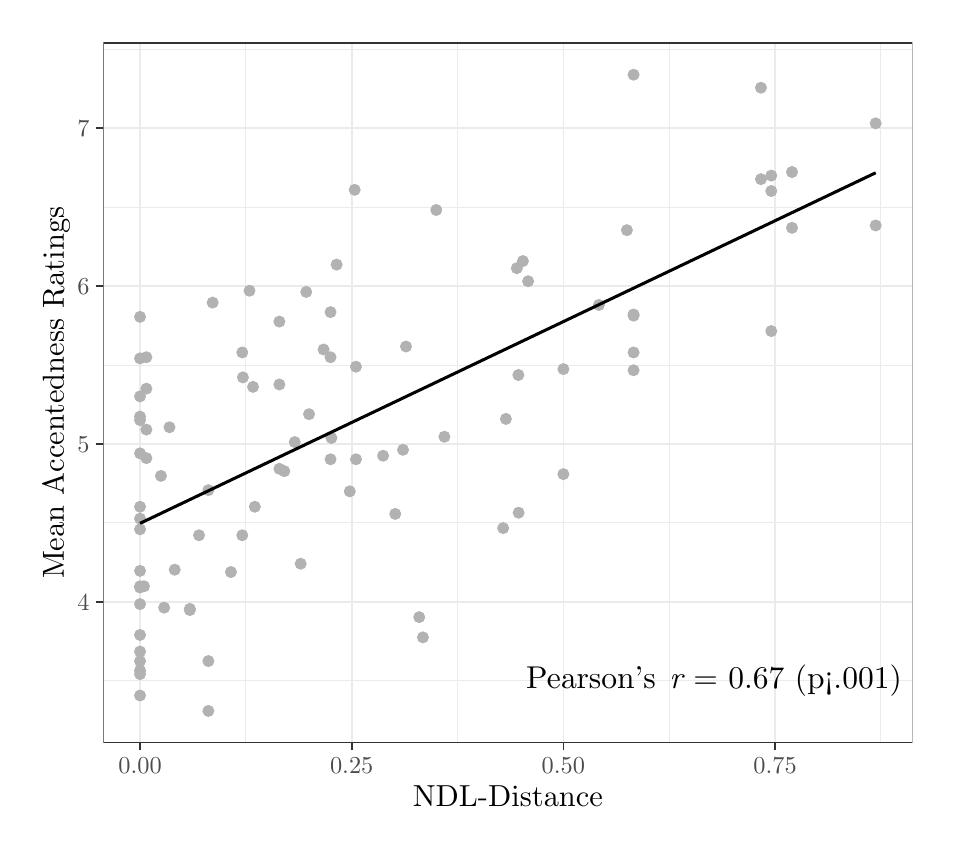
\begin{tikzpicture}[x=1pt,y=1pt]
\definecolor{fillColor}{RGB}{255,255,255}
\path[use as bounding box,fill=fillColor,fill opacity=0.00] (0,0) rectangle (325.21,289.08);
\begin{scope}
\path[clip] (  0.00,  0.00) rectangle (325.21,289.08);
\definecolor{drawColor}{RGB}{255,255,255}
\definecolor{fillColor}{RGB}{255,255,255}

\path[draw=drawColor,line width= 0.6pt,line join=round,line cap=round,fill=fillColor] (  0.00,  0.00) rectangle (325.21,289.08);
\end{scope}
\begin{scope}
\path[clip] ( 27.31, 30.69) rectangle (319.71,283.58);
\definecolor{fillColor}{RGB}{255,255,255}

\path[fill=fillColor] ( 27.31, 30.69) rectangle (319.71,283.58);
\definecolor{drawColor}{gray}{0.92}

\path[draw=drawColor,line width= 0.3pt,line join=round] ( 27.31, 53.12) --
	(319.71, 53.12);

\path[draw=drawColor,line width= 0.3pt,line join=round] ( 27.31,110.17) --
	(319.71,110.17);

\path[draw=drawColor,line width= 0.3pt,line join=round] ( 27.31,167.21) --
	(319.71,167.21);

\path[draw=drawColor,line width= 0.3pt,line join=round] ( 27.31,224.26) --
	(319.71,224.26);

\path[draw=drawColor,line width= 0.3pt,line join=round] ( 27.31,281.31) --
	(319.71,281.31);

\path[draw=drawColor,line width= 0.3pt,line join=round] ( 78.85, 30.69) --
	( 78.85,283.58);

\path[draw=drawColor,line width= 0.3pt,line join=round] (155.34, 30.69) --
	(155.34,283.58);

\path[draw=drawColor,line width= 0.3pt,line join=round] (231.82, 30.69) --
	(231.82,283.58);

\path[draw=drawColor,line width= 0.3pt,line join=round] (308.31, 30.69) --
	(308.31,283.58);

\path[draw=drawColor,line width= 0.6pt,line join=round] ( 27.31, 81.64) --
	(319.71, 81.64);

\path[draw=drawColor,line width= 0.6pt,line join=round] ( 27.31,138.69) --
	(319.71,138.69);

\path[draw=drawColor,line width= 0.6pt,line join=round] ( 27.31,195.74) --
	(319.71,195.74);

\path[draw=drawColor,line width= 0.6pt,line join=round] ( 27.31,252.78) --
	(319.71,252.78);

\path[draw=drawColor,line width= 0.6pt,line join=round] ( 40.60, 30.69) --
	( 40.60,283.58);

\path[draw=drawColor,line width= 0.6pt,line join=round] (117.09, 30.69) --
	(117.09,283.58);

\path[draw=drawColor,line width= 0.6pt,line join=round] (193.58, 30.69) --
	(193.58,283.58);

\path[draw=drawColor,line width= 0.6pt,line join=round] (270.07, 30.69) --
	(270.07,283.58);
\definecolor{drawColor}{gray}{0.70}
\definecolor{fillColor}{gray}{0.70}

\path[draw=drawColor,line width= 0.4pt,line join=round,line cap=round,fill=fillColor] ( 96.50,139.33) circle (  1.96);

\path[draw=drawColor,line width= 0.4pt,line join=round,line cap=round,fill=fillColor] (306.42,217.61) circle (  1.96);

\path[draw=drawColor,line width= 0.4pt,line join=round,line cap=round,fill=fillColor] (118.62,133.11) circle (  1.96);

\path[draw=drawColor,line width= 0.4pt,line join=round,line cap=round,fill=fillColor] ( 61.91,105.66) circle (  1.96);

\path[draw=drawColor,line width= 0.4pt,line join=round,line cap=round,fill=fillColor] (218.94,185.44) circle (  1.96);

\path[draw=drawColor,line width= 0.4pt,line join=round,line cap=round,fill=fillColor] ( 40.60, 60.20) circle (  1.96);

\path[draw=drawColor,line width= 0.4pt,line join=round,line cap=round,fill=fillColor] (136.70,173.86) circle (  1.96);

\path[draw=drawColor,line width= 0.4pt,line join=round,line cap=round,fill=fillColor] (218.94,171.72) circle (  1.96);

\path[draw=drawColor,line width= 0.4pt,line join=round,line cap=round,fill=fillColor] ( 58.60, 79.07) circle (  1.96);

\path[draw=drawColor,line width= 0.4pt,line join=round,line cap=round,fill=fillColor] (106.93,172.79) circle (  1.96);

\path[draw=drawColor,line width= 0.4pt,line join=round,line cap=round,fill=fillColor] (306.42,254.50) circle (  1.96);

\path[draw=drawColor,line width= 0.4pt,line join=round,line cap=round,fill=fillColor] ( 77.54,171.72) circle (  1.96);

\path[draw=drawColor,line width= 0.4pt,line join=round,line cap=round,fill=fillColor] ( 66.83,189.73) circle (  1.96);

\path[draw=drawColor,line width= 0.4pt,line join=round,line cap=round,fill=fillColor] (218.94,272.08) circle (  1.96);

\path[draw=drawColor,line width= 0.4pt,line join=round,line cap=round,fill=fillColor] ( 40.60,107.81) circle (  1.96);

\path[draw=drawColor,line width= 0.4pt,line join=round,line cap=round,fill=fillColor] (132.81,113.38) circle (  1.96);

\path[draw=drawColor,line width= 0.4pt,line join=round,line cap=round,fill=fillColor] ( 92.73,128.82) circle (  1.96);

\path[draw=drawColor,line width= 0.4pt,line join=round,line cap=round,fill=fillColor] (264.97,234.34) circle (  1.96);

\path[draw=drawColor,line width= 0.4pt,line join=round,line cap=round,fill=fillColor] ( 42.89,170.00) circle (  1.96);

\path[draw=drawColor,line width= 0.4pt,line join=round,line cap=round,fill=fillColor] ( 40.60,155.85) circle (  1.96);

\path[draw=drawColor,line width= 0.4pt,line join=round,line cap=round,fill=fillColor] (268.70,179.44) circle (  1.96);

\path[draw=drawColor,line width= 0.4pt,line join=round,line cap=round,fill=fillColor] ( 90.95,129.68) circle (  1.96);

\path[draw=drawColor,line width= 0.4pt,line join=round,line cap=round,fill=fillColor] ( 98.65, 95.37) circle (  1.96);

\path[draw=drawColor,line width= 0.4pt,line join=round,line cap=round,fill=fillColor] ( 90.95,160.14) circle (  1.96);

\path[draw=drawColor,line width= 0.4pt,line join=round,line cap=round,fill=fillColor] ( 40.60,184.58) circle (  1.96);

\path[draw=drawColor,line width= 0.4pt,line join=round,line cap=round,fill=fillColor] ( 82.08,115.96) circle (  1.96);

\path[draw=drawColor,line width= 0.4pt,line join=round,line cap=round,fill=fillColor] (141.48, 76.07) circle (  1.96);

\path[draw=drawColor,line width= 0.4pt,line join=round,line cap=round,fill=fillColor] ( 40.60, 56.76) circle (  1.96);

\path[draw=drawColor,line width= 0.4pt,line join=round,line cap=round,fill=fillColor] (177.40,113.81) circle (  1.96);

\path[draw=drawColor,line width= 0.4pt,line join=round,line cap=round,fill=fillColor] ( 40.60, 87.22) circle (  1.96);

\path[draw=drawColor,line width= 0.4pt,line join=round,line cap=round,fill=fillColor] (135.63,136.54) circle (  1.96);

\path[draw=drawColor,line width= 0.4pt,line join=round,line cap=round,fill=fillColor] (177.31,163.57) circle (  1.96);

\path[draw=drawColor,line width= 0.4pt,line join=round,line cap=round,fill=fillColor] (216.53,215.90) circle (  1.96);

\path[draw=drawColor,line width= 0.4pt,line join=round,line cap=round,fill=fillColor] ( 40.60, 80.78) circle (  1.96);

\path[draw=drawColor,line width= 0.4pt,line join=round,line cap=round,fill=fillColor] ( 53.13, 93.22) circle (  1.96);

\path[draw=drawColor,line width= 0.4pt,line join=round,line cap=round,fill=fillColor] ( 40.60,111.67) circle (  1.96);

\path[draw=drawColor,line width= 0.4pt,line join=round,line cap=round,fill=fillColor] ( 49.31, 79.50) circle (  1.96);

\path[draw=drawColor,line width= 0.4pt,line join=round,line cap=round,fill=fillColor] (180.83,197.45) circle (  1.96);

\path[draw=drawColor,line width= 0.4pt,line join=round,line cap=round,fill=fillColor] (109.44,186.30) circle (  1.96);

\path[draw=drawColor,line width= 0.4pt,line join=round,line cap=round,fill=fillColor] (147.64,223.19) circle (  1.96);

\path[draw=drawColor,line width= 0.4pt,line join=round,line cap=round,fill=fillColor] (218.94,165.28) circle (  1.96);

\path[draw=drawColor,line width= 0.4pt,line join=round,line cap=round,fill=fillColor] (268.70,235.63) circle (  1.96);

\path[draw=drawColor,line width= 0.4pt,line join=round,line cap=round,fill=fillColor] (118.62,166.57) circle (  1.96);

\path[draw=drawColor,line width= 0.4pt,line join=round,line cap=round,fill=fillColor] ( 81.43,159.28) circle (  1.96);

\path[draw=drawColor,line width= 0.4pt,line join=round,line cap=round,fill=fillColor] (118.16,230.48) circle (  1.96);

\path[draw=drawColor,line width= 0.4pt,line join=round,line cap=round,fill=fillColor] (109.44,133.11) circle (  1.96);

\path[draw=drawColor,line width= 0.4pt,line join=round,line cap=round,fill=fillColor] ( 58.60, 78.64) circle (  1.96);

\path[draw=drawColor,line width= 0.4pt,line join=round,line cap=round,fill=fillColor] ( 40.60, 47.76) circle (  1.96);

\path[draw=drawColor,line width= 0.4pt,line join=round,line cap=round,fill=fillColor] (109.44,170.00) circle (  1.96);

\path[draw=drawColor,line width= 0.4pt,line join=round,line cap=round,fill=fillColor] ( 42.02, 87.22) circle (  1.96);

\path[draw=drawColor,line width= 0.4pt,line join=round,line cap=round,fill=fillColor] ( 40.60,148.55) circle (  1.96);

\path[draw=drawColor,line width= 0.4pt,line join=round,line cap=round,fill=fillColor] (276.19,236.91) circle (  1.96);

\path[draw=drawColor,line width= 0.4pt,line join=round,line cap=round,fill=fillColor] (206.42,188.87) circle (  1.96);

\path[draw=drawColor,line width= 0.4pt,line join=round,line cap=round,fill=fillColor] ( 77.54,105.66) circle (  1.96);

\path[draw=drawColor,line width= 0.4pt,line join=round,line cap=round,fill=fillColor] (176.75,202.17) circle (  1.96);

\path[draw=drawColor,line width= 0.4pt,line join=round,line cap=round,fill=fillColor] (101.66,149.41) circle (  1.96);

\path[draw=drawColor,line width= 0.4pt,line join=round,line cap=round,fill=fillColor] (193.58,127.75) circle (  1.96);

\path[draw=drawColor,line width= 0.4pt,line join=round,line cap=round,fill=fillColor] ( 40.60,115.96) circle (  1.96);

\path[draw=drawColor,line width= 0.4pt,line join=round,line cap=round,fill=fillColor] (116.39,121.53) circle (  1.96);

\path[draw=drawColor,line width= 0.4pt,line join=round,line cap=round,fill=fillColor] ( 40.60, 69.63) circle (  1.96);

\path[draw=drawColor,line width= 0.4pt,line join=round,line cap=round,fill=fillColor] ( 42.89,133.54) circle (  1.96);

\path[draw=drawColor,line width= 0.4pt,line join=round,line cap=round,fill=fillColor] (128.44,134.40) circle (  1.96);

\path[draw=drawColor,line width= 0.4pt,line join=round,line cap=round,fill=fillColor] (172.80,147.70) circle (  1.96);

\path[draw=drawColor,line width= 0.4pt,line join=round,line cap=round,fill=fillColor] ( 40.60,135.26) circle (  1.96);

\path[draw=drawColor,line width= 0.4pt,line join=round,line cap=round,fill=fillColor] ( 40.60,169.57) circle (  1.96);

\path[draw=drawColor,line width= 0.4pt,line join=round,line cap=round,fill=fillColor] (111.63,203.46) circle (  1.96);

\path[draw=drawColor,line width= 0.4pt,line join=round,line cap=round,fill=fillColor] ( 90.95,182.87) circle (  1.96);

\path[draw=drawColor,line width= 0.4pt,line join=round,line cap=round,fill=fillColor] (100.65,193.59) circle (  1.96);

\path[draw=drawColor,line width= 0.4pt,line join=round,line cap=round,fill=fillColor] (218.94,185.01) circle (  1.96);

\path[draw=drawColor,line width= 0.4pt,line join=round,line cap=round,fill=fillColor] ( 73.45, 92.37) circle (  1.96);

\path[draw=drawColor,line width= 0.4pt,line join=round,line cap=round,fill=fillColor] ( 40.60, 86.79) circle (  1.96);

\path[draw=drawColor,line width= 0.4pt,line join=round,line cap=round,fill=fillColor] ( 48.16,127.11) circle (  1.96);

\path[draw=drawColor,line width= 0.4pt,line join=round,line cap=round,fill=fillColor] (142.82, 68.77) circle (  1.96);

\path[draw=drawColor,line width= 0.4pt,line join=round,line cap=round,fill=fillColor] (264.97,267.37) circle (  1.96);

\path[draw=drawColor,line width= 0.4pt,line join=round,line cap=round,fill=fillColor] ( 80.15,194.02) circle (  1.96);

\path[draw=drawColor,line width= 0.4pt,line join=round,line cap=round,fill=fillColor] ( 40.60, 63.63) circle (  1.96);

\path[draw=drawColor,line width= 0.4pt,line join=round,line cap=round,fill=fillColor] ( 40.60, 92.79) circle (  1.96);

\path[draw=drawColor,line width= 0.4pt,line join=round,line cap=round,fill=fillColor] ( 40.60,147.27) circle (  1.96);

\path[draw=drawColor,line width= 0.4pt,line join=round,line cap=round,fill=fillColor] ( 77.78,162.71) circle (  1.96);

\path[draw=drawColor,line width= 0.4pt,line join=round,line cap=round,fill=fillColor] (171.82,108.24) circle (  1.96);

\path[draw=drawColor,line width= 0.4pt,line join=round,line cap=round,fill=fillColor] ( 42.89,143.84) circle (  1.96);

\path[draw=drawColor,line width= 0.4pt,line join=round,line cap=round,fill=fillColor] ( 65.29, 60.20) circle (  1.96);

\path[draw=drawColor,line width= 0.4pt,line join=round,line cap=round,fill=fillColor] (276.19,216.75) circle (  1.96);

\path[draw=drawColor,line width= 0.4pt,line join=round,line cap=round,fill=fillColor] (193.58,165.71) circle (  1.96);

\path[draw=drawColor,line width= 0.4pt,line join=round,line cap=round,fill=fillColor] ( 42.89,158.63) circle (  1.96);

\path[draw=drawColor,line width= 0.4pt,line join=round,line cap=round,fill=fillColor] ( 40.60, 55.48) circle (  1.96);

\path[draw=drawColor,line width= 0.4pt,line join=round,line cap=round,fill=fillColor] (178.95,204.74) circle (  1.96);

\path[draw=drawColor,line width= 0.4pt,line join=round,line cap=round,fill=fillColor] ( 51.25,144.69) circle (  1.96);

\path[draw=drawColor,line width= 0.4pt,line join=round,line cap=round,fill=fillColor] (268.70,230.05) circle (  1.96);

\path[draw=drawColor,line width= 0.4pt,line join=round,line cap=round,fill=fillColor] (150.58,141.26) circle (  1.96);

\path[draw=drawColor,line width= 0.4pt,line join=round,line cap=round,fill=fillColor] ( 65.29, 42.18) circle (  1.96);

\path[draw=drawColor,line width= 0.4pt,line join=round,line cap=round,fill=fillColor] ( 65.29,121.96) circle (  1.96);

\path[draw=drawColor,line width= 0.4pt,line join=round,line cap=round,fill=fillColor] (109.76,140.83) circle (  1.96);
\definecolor{drawColor}{RGB}{0,0,0}

\path[draw=drawColor,line width= 1.1pt,line join=round] ( 40.60,109.96) --
	( 43.97,111.57) --
	( 47.33,113.17) --
	( 50.70,114.78) --
	( 54.06,116.38) --
	( 57.43,117.98) --
	( 60.79,119.59) --
	( 64.16,121.19) --
	( 67.52,122.79) --
	( 70.89,124.40) --
	( 74.25,126.00) --
	( 77.62,127.60) --
	( 80.98,129.21) --
	( 84.35,130.81) --
	( 87.71,132.41) --
	( 91.08,134.02) --
	( 94.44,135.62) --
	( 97.81,137.22) --
	(101.17,138.83) --
	(104.54,140.43) --
	(107.90,142.03) --
	(111.27,143.64) --
	(114.63,145.24) --
	(117.99,146.85) --
	(121.36,148.45) --
	(124.72,150.05) --
	(128.09,151.66) --
	(131.45,153.26) --
	(134.82,154.86) --
	(138.18,156.47) --
	(141.55,158.07) --
	(144.91,159.67) --
	(148.28,161.28) --
	(151.64,162.88) --
	(155.01,164.48) --
	(158.37,166.09) --
	(161.74,167.69) --
	(165.10,169.29) --
	(168.47,170.90) --
	(171.83,172.50) --
	(175.20,174.10) --
	(178.56,175.71) --
	(181.93,177.31) --
	(185.29,178.92) --
	(188.66,180.52) --
	(192.02,182.12) --
	(195.39,183.73) --
	(198.75,185.33) --
	(202.11,186.93) --
	(205.48,188.54) --
	(208.84,190.14) --
	(212.21,191.74) --
	(215.57,193.35) --
	(218.94,194.95) --
	(222.30,196.55) --
	(225.67,198.16) --
	(229.03,199.76) --
	(232.40,201.36) --
	(235.76,202.97) --
	(239.13,204.57) --
	(242.49,206.17) --
	(245.86,207.78) --
	(249.22,209.38) --
	(252.59,210.99) --
	(255.95,212.59) --
	(259.32,214.19) --
	(262.68,215.80) --
	(266.05,217.40) --
	(269.41,219.00) --
	(272.78,220.61) --
	(276.14,222.21) --
	(279.51,223.81) --
	(282.87,225.42) --
	(286.24,227.02) --
	(289.60,228.62) --
	(292.96,230.23) --
	(296.33,231.83) --
	(299.69,233.43) --
	(303.06,235.04) --
	(306.42,236.64);

\node[text=drawColor,anchor=base west,inner sep=0pt, outer sep=0pt, scale=  1.14] at (180.13, 50.27) {Pearson's};

\node[text=drawColor,anchor=base west,inner sep=0pt, outer sep=0pt, scale=  1.14] at (231.90, 50.27) {\itshape  r};

\node[text=drawColor,anchor=base west,inner sep=0pt, outer sep=0pt, scale=  1.14] at (240.51, 50.27) { = 0.67 (p<.001)};
\definecolor{drawColor}{gray}{0.20}

\path[draw=drawColor,line width= 0.6pt,line join=round,line cap=round] ( 27.31, 30.69) rectangle (319.71,283.58);
\end{scope}
\begin{scope}
\path[clip] (  0.00,  0.00) rectangle (325.21,289.08);
\definecolor{drawColor}{gray}{0.30}

\node[text=drawColor,anchor=base east,inner sep=0pt, outer sep=0pt, scale=  0.88] at ( 22.36, 78.61) {4};

\node[text=drawColor,anchor=base east,inner sep=0pt, outer sep=0pt, scale=  0.88] at ( 22.36,135.66) {5};

\node[text=drawColor,anchor=base east,inner sep=0pt, outer sep=0pt, scale=  0.88] at ( 22.36,192.71) {6};

\node[text=drawColor,anchor=base east,inner sep=0pt, outer sep=0pt, scale=  0.88] at ( 22.36,249.75) {7};
\end{scope}
\begin{scope}
\path[clip] (  0.00,  0.00) rectangle (325.21,289.08);
\definecolor{drawColor}{gray}{0.20}

\path[draw=drawColor,line width= 0.6pt,line join=round] ( 24.56, 81.64) --
	( 27.31, 81.64);

\path[draw=drawColor,line width= 0.6pt,line join=round] ( 24.56,138.69) --
	( 27.31,138.69);

\path[draw=drawColor,line width= 0.6pt,line join=round] ( 24.56,195.74) --
	( 27.31,195.74);

\path[draw=drawColor,line width= 0.6pt,line join=round] ( 24.56,252.78) --
	( 27.31,252.78);
\end{scope}
\begin{scope}
\path[clip] (  0.00,  0.00) rectangle (325.21,289.08);
\definecolor{drawColor}{gray}{0.20}

\path[draw=drawColor,line width= 0.6pt,line join=round] ( 40.60, 27.94) --
	( 40.60, 30.69);

\path[draw=drawColor,line width= 0.6pt,line join=round] (117.09, 27.94) --
	(117.09, 30.69);

\path[draw=drawColor,line width= 0.6pt,line join=round] (193.58, 27.94) --
	(193.58, 30.69);

\path[draw=drawColor,line width= 0.6pt,line join=round] (270.07, 27.94) --
	(270.07, 30.69);
\end{scope}
\begin{scope}
\path[clip] (  0.00,  0.00) rectangle (325.21,289.08);
\definecolor{drawColor}{gray}{0.30}

\node[text=drawColor,anchor=base,inner sep=0pt, outer sep=0pt, scale=  0.88] at ( 40.60, 19.68) {0.00};

\node[text=drawColor,anchor=base,inner sep=0pt, outer sep=0pt, scale=  0.88] at (117.09, 19.68) {0.25};

\node[text=drawColor,anchor=base,inner sep=0pt, outer sep=0pt, scale=  0.88] at (193.58, 19.68) {0.50};

\node[text=drawColor,anchor=base,inner sep=0pt, outer sep=0pt, scale=  0.88] at (270.07, 19.68) {0.75};
\end{scope}
\begin{scope}
\path[clip] (  0.00,  0.00) rectangle (325.21,289.08);
\definecolor{drawColor}{RGB}{0,0,0}

\node[text=drawColor,anchor=base,inner sep=0pt, outer sep=0pt, scale=  1.10] at (173.51,  7.64) {NDL-Distance};
\end{scope}
\begin{scope}
\path[clip] (  0.00,  0.00) rectangle (325.21,289.08);
\definecolor{drawColor}{RGB}{0,0,0}

\node[text=drawColor,rotate= 90.00,anchor=base,inner sep=0pt, outer sep=0pt, scale=  1.10] at ( 13.08,157.13) {Mean Accentedness Ratings};
\end{scope}
\end{tikzpicture}

	%\includegraphics[width=0.75\textwidth]{figures/ndl/all.png}
    \caption{Relationship between Accentedness and NDL-Distance}
    \label{fig:all}
  \figSpace
\end{figure}

Overall, there is a clear positive relationship between the accentedness ratings and the NDL-distances (Pearson’s r = .67, p <.001). This result generally agrees with the prediction that the larger the NDL-distance between an L2 stimulus and its corresponding L1 productions, the more accented the L2 stimulus will be judged.

\subsubsection{Types of Mismatches}

Linear mixed-effects regression models were constructed to investigate the effects of the four types of stimuli (i.e., consonant vs. syllable vs. vowel vs. match), while controlling for NDL-distances. Rating data from Experiment 2 were used for the analysis. Accentednss ratings were the dependent variable. Helmert-contrast-coding was again performed on the “types of stimuli” variable to create three contrasts. The first contrast compares stimuli with consonant mismatches and stimuli with syllable mismatches, the second contrast compares vowel mismatches with consonant and syllable mismatches, and the third contrast compares the match stimuli with the three types of mismatch stimuli. The three contrasts, trial numbers and NDL-distances for the stimuli were entered as fixed effects. Two-way and three-way interactions of the fixed effects were also entered as fixed effects. Raters and stimuli were entered as random effects.

Model comparisons using likelihood ratio tests showed that (1) NDL-distances significantly contributed to model fit ($\beta$ = 1.74, χ2 = 8.79, p<.01), showing that the degree of dissimilarity between L1 and L2 speech samples could have affected accentedness perception; (2) trial number contributed significantly to model fit ($\beta$ = 0.6, χ2 = 72.24, p<.001), showing that the accentedness ratings increased overtime; and (3) the three contrasts did not contribute significantly to model fit, showing that accentedness differences between the four types of stimuli diminished once NDL-distances were controlled for.

To further investigate the interactions between NDL-distances and the types of mismatches, mean accentedness ratings of each type of mismatch were plotted against NDL-distances. Figure \ref{fig:con} demonstrates the relationship between NDL-distances and accentedness ratings of stimuli with consonant and syllable mismatches.

\begin{figure}[!h]
  \figSpace
    \centering
    % Created by tikzDevice version 0.12.3 on 2019-11-25 15:09:07
% !TEX encoding = UTF-8 Unicode
\begin{tikzpicture}[x=1pt,y=1pt]
\definecolor{fillColor}{RGB}{255,255,255}
\path[use as bounding box,fill=fillColor,fill opacity=0.00] (0,0) rectangle (325.21,289.08);
\begin{scope}
\path[clip] (  0.00,  0.00) rectangle (325.21,289.08);
\definecolor{drawColor}{RGB}{255,255,255}
\definecolor{fillColor}{RGB}{255,255,255}

\path[draw=drawColor,line width= 0.6pt,line join=round,line cap=round,fill=fillColor] (  0.00,  0.00) rectangle (325.21,289.08);
\end{scope}
\begin{scope}
\path[clip] ( 27.31, 30.69) rectangle (319.71,267.01);
\definecolor{fillColor}{RGB}{255,255,255}

\path[fill=fillColor] ( 27.31, 30.69) rectangle (319.71,267.01);
\definecolor{drawColor}{gray}{0.92}

\path[draw=drawColor,line width= 0.3pt,line join=round] ( 27.31, 65.30) --
	(319.71, 65.30);

\path[draw=drawColor,line width= 0.3pt,line join=round] ( 27.31,113.04) --
	(319.71,113.04);

\path[draw=drawColor,line width= 0.3pt,line join=round] ( 27.31,160.78) --
	(319.71,160.78);

\path[draw=drawColor,line width= 0.3pt,line join=round] ( 27.31,208.52) --
	(319.71,208.52);

\path[draw=drawColor,line width= 0.3pt,line join=round] ( 27.31,256.27) --
	(319.71,256.27);

\path[draw=drawColor,line width= 0.3pt,line join=round] ( 73.83, 30.69) --
	( 73.83,267.01);

\path[draw=drawColor,line width= 0.3pt,line join=round] (140.29, 30.69) --
	(140.29,267.01);

\path[draw=drawColor,line width= 0.3pt,line join=round] (206.74, 30.69) --
	(206.74,267.01);

\path[draw=drawColor,line width= 0.3pt,line join=round] (273.20, 30.69) --
	(273.20,267.01);

\path[draw=drawColor,line width= 0.6pt,line join=round] ( 27.31, 41.43) --
	(319.71, 41.43);

\path[draw=drawColor,line width= 0.6pt,line join=round] ( 27.31, 89.17) --
	(319.71, 89.17);

\path[draw=drawColor,line width= 0.6pt,line join=round] ( 27.31,136.91) --
	(319.71,136.91);

\path[draw=drawColor,line width= 0.6pt,line join=round] ( 27.31,184.65) --
	(319.71,184.65);

\path[draw=drawColor,line width= 0.6pt,line join=round] ( 27.31,232.40) --
	(319.71,232.40);

\path[draw=drawColor,line width= 0.6pt,line join=round] ( 40.60, 30.69) --
	( 40.60,267.01);

\path[draw=drawColor,line width= 0.6pt,line join=round] (107.06, 30.69) --
	(107.06,267.01);

\path[draw=drawColor,line width= 0.6pt,line join=round] (173.51, 30.69) --
	(173.51,267.01);

\path[draw=drawColor,line width= 0.6pt,line join=round] (239.97, 30.69) --
	(239.97,267.01);

\path[draw=drawColor,line width= 0.6pt,line join=round] (306.42, 30.69) --
	(306.42,267.01);
\definecolor{fillColor}{gray}{0.10}

\path[fill=fillColor] ( 89.17,137.45) circle (  1.96);

\path[fill=fillColor] (271.56,202.96) circle (  1.96);

\path[fill=fillColor] ( 59.11,109.27) circle (  1.96);

\path[fill=fillColor] (195.55,176.04) circle (  1.96);

\path[fill=fillColor] (195.55,164.55) circle (  1.96);

\path[fill=fillColor] (271.56,233.83) circle (  1.96);

\path[fill=fillColor] ( 72.69,164.55) circle (  1.96);

\path[fill=fillColor] (195.55,248.55) circle (  1.96);

\path[fill=fillColor] (193.45,201.52) circle (  1.96);

\path[fill=fillColor] (133.60,207.63) circle (  1.96);

\path[fill=fillColor] (195.55,159.17) circle (  1.96);

\path[fill=fillColor] (107.99,213.73) circle (  1.96);

\path[fill=fillColor] (184.67,178.91) circle (  1.96);

\path[fill=fillColor] ( 72.69,109.27) circle (  1.96);

\path[fill=fillColor] (116.92,133.32) circle (  1.96);

\path[fill=fillColor] (155.46,144.45) circle (  1.96);

\path[fill=fillColor] (102.31,191.11) circle (  1.96);

\path[fill=fillColor] (195.55,175.68) circle (  1.96);

\path[fill=fillColor] ( 72.91,157.01) circle (  1.96);

\path[fill=fillColor] (154.60,111.43) circle (  1.96);

\path[fill=fillColor] (160.80,192.19) circle (  1.96);

\path[fill=fillColor] (100.69,138.71) circle (  1.96);
\definecolor{drawColor}{RGB}{26,26,26}

\node[text=drawColor,text opacity=0.80,anchor=base,inner sep=0pt, outer sep=0pt, scale=  0.85] at ( 89.17,130.57) {kʰ$\rightarrow$k};

\node[text=drawColor,text opacity=0.80,anchor=base,inner sep=0pt, outer sep=0pt, scale=  0.85] at (271.56,197.08) {pʰl$\rightarrow$pl};

\node[text=drawColor,text opacity=0.80,anchor=base,inner sep=0pt, outer sep=0pt, scale=  0.85] at ( 59.11,103.39) {pʰl$\rightarrow$pl};

\node[text=drawColor,text opacity=0.80,anchor=base,inner sep=0pt, outer sep=0pt, scale=  0.85] at (195.55,170.16) {ɹ$\rightarrow$r};

\node[text=drawColor,text opacity=0.80,anchor=base,inner sep=0pt, outer sep=0pt, scale=  0.85] at (195.55,158.67) {ɹ$\rightarrow$r};

\node[text=drawColor,text opacity=0.80,anchor=base,inner sep=0pt, outer sep=0pt, scale=  0.85] at (271.56,227.95) {pʰl$\rightarrow$pl};

\node[text=drawColor,text opacity=0.80,anchor=base,inner sep=0pt, outer sep=0pt, scale=  0.85] at ( 72.69,158.67) {θ$\rightarrow$t̪};

\node[text=drawColor,text opacity=0.80,anchor=base,inner sep=0pt, outer sep=0pt, scale=  0.85] at (195.55,242.67) {ɹ$\rightarrow$r};

\node[text=drawColor,text opacity=0.80,anchor=base,inner sep=0pt, outer sep=0pt, scale=  0.85] at (193.45,195.65) {θ$\rightarrow$st};

\node[text=drawColor,text opacity=0.80,anchor=base,inner sep=0pt, outer sep=0pt, scale=  0.85] at (133.60,201.75) {pʰl$\rightarrow$pʰll};

\node[text=drawColor,text opacity=0.80,anchor=base,inner sep=0pt, outer sep=0pt, scale=  0.85] at (195.55,153.29) {ɹ$\rightarrow$r};

\node[text=drawColor,text opacity=0.80,anchor=base,inner sep=0pt, outer sep=0pt, scale=  0.85] at (107.99,207.85) {pʰl$\rightarrow$pʰɾ};

\node[text=drawColor,text opacity=0.80,anchor=base,inner sep=0pt, outer sep=0pt, scale=  0.85] at (184.67,173.03) {spũnz$\rightarrow$spũnʃ};

\node[text=drawColor,text opacity=0.80,anchor=base,inner sep=0pt, outer sep=0pt, scale=  0.85] at ( 72.69,103.39) {θ$\rightarrow$t̪};

\node[text=drawColor,text opacity=0.80,anchor=base,inner sep=0pt, outer sep=0pt, scale=  0.85] at (116.92,127.44) {θ$\rightarrow$f};

\node[text=drawColor,text opacity=0.80,anchor=base,inner sep=0pt, outer sep=0pt, scale=  0.85] at (155.46,138.57) {sm$\rightarrow$zm};

\node[text=drawColor,text opacity=0.80,anchor=base,inner sep=0pt, outer sep=0pt, scale=  0.85] at (102.31,185.24) {smɑl$\rightarrow$smɑɭ};

\node[text=drawColor,text opacity=0.80,anchor=base,inner sep=0pt, outer sep=0pt, scale=  0.85] at (195.55,169.80) {ɹ$\rightarrow$r};

\node[text=drawColor,text opacity=0.80,anchor=base,inner sep=0pt, outer sep=0pt, scale=  0.85] at ( 72.91,151.13) {θ$\rightarrow$t̪};

\node[text=drawColor,text opacity=0.80,anchor=base,inner sep=0pt, outer sep=0pt, scale=  0.85] at (154.60,105.55) {sp$\rightarrow$spʰ};

\node[text=drawColor,text opacity=0.80,anchor=base,inner sep=0pt, outer sep=0pt, scale=  0.85] at (160.80,186.31) {sp$\rightarrow$spʰ};

\node[text=drawColor,text opacity=0.80,anchor=base,inner sep=0pt, outer sep=0pt, scale=  0.85] at (100.69,138.83) {pʰliz$\rightarrow$pʰlis};
\definecolor{drawColor}{RGB}{0,0,0}

\path[draw=drawColor,line width= 1.1pt,line join=round] ( 59.11,137.33) --
	( 61.80,138.32) --
	( 64.49,139.30) --
	( 67.18,140.28) --
	( 69.87,141.26) --
	( 72.56,142.25) --
	( 75.25,143.23) --
	( 77.94,144.21) --
	( 80.63,145.20) --
	( 83.32,146.18) --
	( 86.00,147.16) --
	( 88.69,148.14) --
	( 91.38,149.13) --
	( 94.07,150.11) --
	( 96.76,151.09) --
	( 99.45,152.08) --
	(102.14,153.06) --
	(104.83,154.04) --
	(107.52,155.02) --
	(110.21,156.01) --
	(112.90,156.99) --
	(115.59,157.97) --
	(118.27,158.95) --
	(120.96,159.94) --
	(123.65,160.92) --
	(126.34,161.90) --
	(129.03,162.89) --
	(131.72,163.87) --
	(134.41,164.85) --
	(137.10,165.83) --
	(139.79,166.82) --
	(142.48,167.80) --
	(145.17,168.78) --
	(147.85,169.77) --
	(150.54,170.75) --
	(153.23,171.73) --
	(155.92,172.71) --
	(158.61,173.70) --
	(161.30,174.68) --
	(163.99,175.66) --
	(166.68,176.65) --
	(169.37,177.63) --
	(172.06,178.61) --
	(174.75,179.59) --
	(177.44,180.58) --
	(180.12,181.56) --
	(182.81,182.54) --
	(185.50,183.53) --
	(188.19,184.51) --
	(190.88,185.49) --
	(193.57,186.47) --
	(196.26,187.46) --
	(198.95,188.44) --
	(201.64,189.42) --
	(204.33,190.41) --
	(207.02,191.39) --
	(209.71,192.37) --
	(212.39,193.35) --
	(215.08,194.34) --
	(217.77,195.32) --
	(220.46,196.30) --
	(223.15,197.28) --
	(225.84,198.27) --
	(228.53,199.25) --
	(231.22,200.23) --
	(233.91,201.22) --
	(236.60,202.20) --
	(239.29,203.18) --
	(241.97,204.16) --
	(244.66,205.15) --
	(247.35,206.13) --
	(250.04,207.11) --
	(252.73,208.10) --
	(255.42,209.08) --
	(258.11,210.06) --
	(260.80,211.04) --
	(263.49,212.03) --
	(266.18,213.01) --
	(268.87,213.99) --
	(271.56,214.98);

\node[text=drawColor,anchor=base west,inner sep=0pt, outer sep=0pt, scale=  1.14] at (155.88, 62.45) {Pearson's};

\node[text=drawColor,anchor=base west,inner sep=0pt, outer sep=0pt, scale=  1.14] at (207.66, 62.45) {\itshape  r};

\node[text=drawColor,anchor=base west,inner sep=0pt, outer sep=0pt, scale=  1.14] at (217.26, 62.45) { = 0.58 (p<.01)};
\definecolor{drawColor}{gray}{0.20}

\path[draw=drawColor,line width= 0.6pt,line join=round,line cap=round] ( 27.31, 30.69) rectangle (319.71,267.01);
\end{scope}
\begin{scope}
\path[clip] ( 27.31,267.01) rectangle (319.71,283.58);
\definecolor{drawColor}{gray}{0.20}
\definecolor{fillColor}{gray}{0.85}

\path[draw=drawColor,line width= 0.6pt,line join=round,line cap=round,fill=fillColor] ( 27.31,267.01) rectangle (319.71,283.58);
\definecolor{drawColor}{gray}{0.10}

\node[text=drawColor,anchor=base,inner sep=0pt, outer sep=0pt, scale=  0.88] at (173.51,272.26) {Consonant};
\end{scope}
\begin{scope}
\path[clip] (  0.00,  0.00) rectangle (325.21,289.08);
\definecolor{drawColor}{gray}{0.20}

\path[draw=drawColor,line width= 0.6pt,line join=round] ( 40.60, 27.94) --
	( 40.60, 30.69);

\path[draw=drawColor,line width= 0.6pt,line join=round] (107.06, 27.94) --
	(107.06, 30.69);

\path[draw=drawColor,line width= 0.6pt,line join=round] (173.51, 27.94) --
	(173.51, 30.69);

\path[draw=drawColor,line width= 0.6pt,line join=round] (239.97, 27.94) --
	(239.97, 30.69);

\path[draw=drawColor,line width= 0.6pt,line join=round] (306.42, 27.94) --
	(306.42, 30.69);
\end{scope}
\begin{scope}
\path[clip] (  0.00,  0.00) rectangle (325.21,289.08);
\definecolor{drawColor}{gray}{0.30}

\node[text=drawColor,anchor=base,inner sep=0pt, outer sep=0pt, scale=  0.88] at ( 40.60, 19.68) {0.00};

\node[text=drawColor,anchor=base,inner sep=0pt, outer sep=0pt, scale=  0.88] at (107.06, 19.68) {0.25};

\node[text=drawColor,anchor=base,inner sep=0pt, outer sep=0pt, scale=  0.88] at (173.51, 19.68) {0.50};

\node[text=drawColor,anchor=base,inner sep=0pt, outer sep=0pt, scale=  0.88] at (239.97, 19.68) {0.75};

\node[text=drawColor,anchor=base,inner sep=0pt, outer sep=0pt, scale=  0.88] at (306.42, 19.68) {1.00};
\end{scope}
\begin{scope}
\path[clip] (  0.00,  0.00) rectangle (325.21,289.08);
\definecolor{drawColor}{gray}{0.30}

\node[text=drawColor,anchor=base east,inner sep=0pt, outer sep=0pt, scale=  0.88] at ( 22.36, 38.40) {3};

\node[text=drawColor,anchor=base east,inner sep=0pt, outer sep=0pt, scale=  0.88] at ( 22.36, 86.14) {4};

\node[text=drawColor,anchor=base east,inner sep=0pt, outer sep=0pt, scale=  0.88] at ( 22.36,133.88) {5};

\node[text=drawColor,anchor=base east,inner sep=0pt, outer sep=0pt, scale=  0.88] at ( 22.36,181.62) {6};

\node[text=drawColor,anchor=base east,inner sep=0pt, outer sep=0pt, scale=  0.88] at ( 22.36,229.37) {7};
\end{scope}
\begin{scope}
\path[clip] (  0.00,  0.00) rectangle (325.21,289.08);
\definecolor{drawColor}{gray}{0.20}

\path[draw=drawColor,line width= 0.6pt,line join=round] ( 24.56, 41.43) --
	( 27.31, 41.43);

\path[draw=drawColor,line width= 0.6pt,line join=round] ( 24.56, 89.17) --
	( 27.31, 89.17);

\path[draw=drawColor,line width= 0.6pt,line join=round] ( 24.56,136.91) --
	( 27.31,136.91);

\path[draw=drawColor,line width= 0.6pt,line join=round] ( 24.56,184.65) --
	( 27.31,184.65);

\path[draw=drawColor,line width= 0.6pt,line join=round] ( 24.56,232.40) --
	( 27.31,232.40);
\end{scope}
\begin{scope}
\path[clip] (  0.00,  0.00) rectangle (325.21,289.08);
\definecolor{drawColor}{RGB}{0,0,0}

\node[text=drawColor,anchor=base,inner sep=0pt, outer sep=0pt, scale=  1.10] at (173.51,  7.64) {NDL-Distance};
\end{scope}
\begin{scope}
\path[clip] (  0.00,  0.00) rectangle (325.21,289.08);
\definecolor{drawColor}{RGB}{0,0,0}

\node[text=drawColor,rotate= 90.00,anchor=base,inner sep=0pt, outer sep=0pt, scale=  1.10] at ( 13.08,148.85) {Mean Accentedness Ratings};
\end{scope}
\end{tikzpicture}

	%\includegraphics[width=1\textwidth]{figures/ndl/con_syl.png}
    \caption{Relationship between Accentedness and NDL-Distance (Consonant)}
    \label{fig:con}
  \figSpace
\end{figure}

Figure \ref{fig:con} shows that the mean accentedness ratings of different types of consonant mismatches positively correlates with NDL-distances (Pearson’s r = 0.58, p<.01). For example, the two instances of VOT-shortening on consonant cluster /pl/ in the context of “\textit{please call}” had an NDL-distance as large as 0.886 and the two instances were judged as being relatively more accented. The instance for VOT-shortening on /pl/ in the context of “\textit{small plastic}” had an NDL-distance as small as 0.070, and it was judged as being less accented. 

\begin{figure}[!h]
  \figSpace
    \centering
    % Created by tikzDevice version 0.12.3 on 2019-11-25 15:43:46
% !TEX encoding = UTF-8 Unicode
\begin{tikzpicture}[x=1pt,y=1pt]
\definecolor{fillColor}{RGB}{255,255,255}
\path[use as bounding box,fill=fillColor,fill opacity=0.00] (0,0) rectangle (339.67,289.08);
\begin{scope}
\path[clip] (  0.00,  0.00) rectangle (339.67,289.08);
\definecolor{drawColor}{RGB}{255,255,255}
\definecolor{fillColor}{RGB}{255,255,255}

\path[draw=drawColor,line width= 0.6pt,line join=round,line cap=round,fill=fillColor] (  0.00,  0.00) rectangle (339.67,289.08);
\end{scope}
\begin{scope}
\path[clip] ( 27.31, 30.69) rectangle (334.17,267.01);
\definecolor{fillColor}{RGB}{255,255,255}

\path[fill=fillColor] ( 27.31, 30.69) rectangle (334.17,267.01);
\definecolor{drawColor}{gray}{0.92}

\path[draw=drawColor,line width= 0.3pt,line join=round] ( 27.31, 65.30) --
	(334.17, 65.30);

\path[draw=drawColor,line width= 0.3pt,line join=round] ( 27.31,113.04) --
	(334.17,113.04);

\path[draw=drawColor,line width= 0.3pt,line join=round] ( 27.31,160.78) --
	(334.17,160.78);

\path[draw=drawColor,line width= 0.3pt,line join=round] ( 27.31,208.52) --
	(334.17,208.52);

\path[draw=drawColor,line width= 0.3pt,line join=round] ( 27.31,256.27) --
	(334.17,256.27);

\path[draw=drawColor,line width= 0.3pt,line join=round] ( 76.13, 30.69) --
	( 76.13,267.01);

\path[draw=drawColor,line width= 0.3pt,line join=round] (145.87, 30.69) --
	(145.87,267.01);

\path[draw=drawColor,line width= 0.3pt,line join=round] (215.61, 30.69) --
	(215.61,267.01);

\path[draw=drawColor,line width= 0.3pt,line join=round] (285.35, 30.69) --
	(285.35,267.01);

\path[draw=drawColor,line width= 0.6pt,line join=round] ( 27.31, 41.43) --
	(334.17, 41.43);

\path[draw=drawColor,line width= 0.6pt,line join=round] ( 27.31, 89.17) --
	(334.17, 89.17);

\path[draw=drawColor,line width= 0.6pt,line join=round] ( 27.31,136.91) --
	(334.17,136.91);

\path[draw=drawColor,line width= 0.6pt,line join=round] ( 27.31,184.65) --
	(334.17,184.65);

\path[draw=drawColor,line width= 0.6pt,line join=round] ( 27.31,232.40) --
	(334.17,232.40);

\path[draw=drawColor,line width= 0.6pt,line join=round] ( 41.26, 30.69) --
	( 41.26,267.01);

\path[draw=drawColor,line width= 0.6pt,line join=round] (111.00, 30.69) --
	(111.00,267.01);

\path[draw=drawColor,line width= 0.6pt,line join=round] (180.74, 30.69) --
	(180.74,267.01);

\path[draw=drawColor,line width= 0.6pt,line join=round] (250.48, 30.69) --
	(250.48,267.01);

\path[draw=drawColor,line width= 0.6pt,line join=round] (320.22, 30.69) --
	(320.22,267.01);
\definecolor{fillColor}{gray}{0.10}

\path[fill=fillColor] (101.73,165.45) circle (  1.96);

\path[fill=fillColor] (125.33,115.73) circle (  1.96);

\path[fill=fillColor] (245.83,216.96) circle (  1.96);

\path[fill=fillColor] ( 43.35,163.12) circle (  1.96);

\path[fill=fillColor] (249.24,171.01) circle (  1.96);

\path[fill=fillColor] (133.24, 84.50) circle (  1.96);

\path[fill=fillColor] (249.24,218.04) circle (  1.96);

\path[fill=fillColor] ( 78.48,154.14) circle (  1.96);

\path[fill=fillColor] (256.06,219.11) circle (  1.96);

\path[fill=fillColor] (110.36,122.55) circle (  1.96);

\path[fill=fillColor] ( 43.35,132.60) circle (  1.96);

\path[fill=fillColor] ( 96.01,182.86) circle (  1.96);

\path[fill=fillColor] ( 71.21, 98.14) circle (  1.96);

\path[fill=fillColor] (245.83,244.60) circle (  1.96);

\path[fill=fillColor] ( 77.32,183.22) circle (  1.96);

\path[fill=fillColor] ( 43.35,141.22) circle (  1.96);

\path[fill=fillColor] ( 63.77, 71.22) circle (  1.96);

\path[fill=fillColor] (256.06,202.24) circle (  1.96);

\path[fill=fillColor] ( 43.35,153.60) circle (  1.96);

\path[fill=fillColor] (249.24,213.37) circle (  1.96);

\path[fill=fillColor] ( 63.77, 56.15) circle (  1.96);

\path[fill=fillColor] ( 63.77,122.91) circle (  1.96);
\definecolor{drawColor}{RGB}{26,26,26}

\node[text=drawColor,text opacity=0.80,anchor=base,inner sep=0pt, outer sep=0pt, scale=  0.85] at (101.73,159.57) {spũnz$\rightarrow$spuz};

\node[text=drawColor,text opacity=0.80,anchor=base,inner sep=0pt, outer sep=0pt, scale=  0.85] at (125.33,109.85) {kʰɑl$\rightarrow$kʰɑ };

\node[text=drawColor,text opacity=0.80,anchor=base,inner sep=0pt, outer sep=0pt, scale=  0.85] at (245.83,211.08) {æsk$\rightarrow$æs};

\node[text=drawColor,text opacity=0.80,anchor=base,inner sep=0pt, outer sep=0pt, scale=  0.85] at ( 43.35,157.24) {pʰlæstɪk$\rightarrow$pʰlæsik};

\node[text=drawColor,text opacity=0.80,anchor=base,inner sep=0pt, outer sep=0pt, scale=  0.85] at (249.24,165.13) {pʰl$\rightarrow$pʰəl};

\node[text=drawColor,text opacity=0.80,anchor=base,inner sep=0pt, outer sep=0pt, scale=  0.85] at (133.24, 78.62) {pʰl$\rightarrow$pʰ};

\node[text=drawColor,text opacity=0.80,anchor=base,inner sep=0pt, outer sep=0pt, scale=  0.85] at (249.24,212.16) {pʰl$\rightarrow$pʰəl};

\node[text=drawColor,text opacity=0.80,anchor=base,inner sep=0pt, outer sep=0pt, scale=  0.85] at ( 78.48,148.26) {faɪv$\rightarrow$faɪvə};

\node[text=drawColor,text opacity=0.80,anchor=base,inner sep=0pt, outer sep=0pt, scale=  0.85] at (256.06,213.24) {æsk$\rightarrow$æskə};

\node[text=drawColor,text opacity=0.80,anchor=base,inner sep=0pt, outer sep=0pt, scale=  0.85] at (110.36,116.67) {spũnz$\rightarrow$spũz};

\node[text=drawColor,text opacity=0.80,anchor=base,inner sep=0pt, outer sep=0pt, scale=  0.85] at ( 43.35,126.73) {pʰlæstɪk$\rightarrow$pʰlæsɪk};

\node[text=drawColor,text opacity=0.80,anchor=base,inner sep=0pt, outer sep=0pt, scale=  0.85] at ( 96.01,176.98) {spũnz$\rightarrow$əspũnz};

\node[text=drawColor,text opacity=0.80,anchor=base,inner sep=0pt, outer sep=0pt, scale=  0.85] at ( 71.21, 92.26) {spũnz$\rightarrow$əspũnz};

\node[text=drawColor,text opacity=0.80,anchor=base,inner sep=0pt, outer sep=0pt, scale=  0.85] at (245.83,238.72) {æsk$\rightarrow$æs};

\node[text=drawColor,text opacity=0.80,anchor=base,inner sep=0pt, outer sep=0pt, scale=  0.85] at ( 77.32,177.34) {faɪv$\rightarrow$faɪ};

\node[text=drawColor,text opacity=0.80,anchor=base,inner sep=0pt, outer sep=0pt, scale=  0.85] at ( 43.35,135.34) {pʰlæstɪk$\rightarrow$plasik};

\node[text=drawColor,text opacity=0.80,anchor=base,inner sep=0pt, outer sep=0pt, scale=  0.85] at ( 63.77, 65.34) {faɪv$\rightarrow$faɪ};

\node[text=drawColor,text opacity=0.80,anchor=base,inner sep=0pt, outer sep=0pt, scale=  0.85] at (256.06,196.36) {æsk$\rightarrow$æskə};

\node[text=drawColor,text opacity=0.80,anchor=base,inner sep=0pt, outer sep=0pt, scale=  0.85] at ( 43.35,147.72) {pʰlæstɪk$\rightarrow$pʰlæsɪk};

\node[text=drawColor,text opacity=0.80,anchor=base,inner sep=0pt, outer sep=0pt, scale=  0.85] at (249.24,207.49) {pʰl$\rightarrow$pʰəl};

\node[text=drawColor,text opacity=0.80,anchor=base,inner sep=0pt, outer sep=0pt, scale=  0.85] at ( 63.77, 50.27) {faɪv$\rightarrow$faɪ};

\node[text=drawColor,text opacity=0.80,anchor=base,inner sep=0pt, outer sep=0pt, scale=  0.85] at ( 63.77,117.03) {faɪv$\rightarrow$faɪ};
\definecolor{drawColor}{RGB}{0,0,0}

\path[draw=drawColor,line width= 1.1pt,line join=round] ( 43.35,118.35) --
	( 46.04,119.49) --
	( 48.73,120.63) --
	( 51.43,121.77) --
	( 54.12,122.91) --
	( 56.81,124.05) --
	( 59.50,125.20) --
	( 62.20,126.34) --
	( 64.89,127.48) --
	( 67.58,128.62) --
	( 70.27,129.76) --
	( 72.97,130.90) --
	( 75.66,132.04) --
	( 78.35,133.18) --
	( 81.04,134.32) --
	( 83.74,135.47) --
	( 86.43,136.61) --
	( 89.12,137.75) --
	( 91.81,138.89) --
	( 94.51,140.03) --
	( 97.20,141.17) --
	( 99.89,142.31) --
	(102.58,143.45) --
	(105.28,144.60) --
	(107.97,145.74) --
	(110.66,146.88) --
	(113.35,148.02) --
	(116.05,149.16) --
	(118.74,150.30) --
	(121.43,151.44) --
	(124.12,152.58) --
	(126.82,153.72) --
	(129.51,154.87) --
	(132.20,156.01) --
	(134.89,157.15) --
	(137.59,158.29) --
	(140.28,159.43) --
	(142.97,160.57) --
	(145.67,161.71) --
	(148.36,162.85) --
	(151.05,164.00) --
	(153.74,165.14) --
	(156.44,166.28) --
	(159.13,167.42) --
	(161.82,168.56) --
	(164.51,169.70) --
	(167.21,170.84) --
	(169.90,171.98) --
	(172.59,173.13) --
	(175.28,174.27) --
	(177.98,175.41) --
	(180.67,176.55) --
	(183.36,177.69) --
	(186.05,178.83) --
	(188.75,179.97) --
	(191.44,181.11) --
	(194.13,182.25) --
	(196.82,183.40) --
	(199.52,184.54) --
	(202.21,185.68) --
	(204.90,186.82) --
	(207.59,187.96) --
	(210.29,189.10) --
	(212.98,190.24) --
	(215.67,191.38) --
	(218.36,192.53) --
	(221.06,193.67) --
	(223.75,194.81) --
	(226.44,195.95) --
	(229.13,197.09) --
	(231.83,198.23) --
	(234.52,199.37) --
	(237.21,200.51) --
	(239.90,201.65) --
	(242.60,202.80) --
	(245.29,203.94) --
	(247.98,205.08) --
	(250.68,206.22) --
	(253.37,207.36) --
	(256.06,208.50);

\node[text=drawColor,anchor=base west,inner sep=0pt, outer sep=0pt, scale=  1.14] at (162.89, 62.45) {Pearson's};

\node[text=drawColor,anchor=base west,inner sep=0pt, outer sep=0pt, scale=  1.14] at (214.67, 62.45) {\itshape  r};

\node[text=drawColor,anchor=base west,inner sep=0pt, outer sep=0pt, scale=  1.14] at (224.27, 62.45) { = 0.69 (p<.001)};
\definecolor{drawColor}{gray}{0.20}

\path[draw=drawColor,line width= 0.6pt,line join=round,line cap=round] ( 27.31, 30.69) rectangle (334.17,267.01);
\end{scope}
\begin{scope}
\path[clip] ( 27.31,267.01) rectangle (334.17,283.58);
\definecolor{drawColor}{gray}{0.20}
\definecolor{fillColor}{gray}{0.85}

\path[draw=drawColor,line width= 0.6pt,line join=round,line cap=round,fill=fillColor] ( 27.31,267.01) rectangle (334.17,283.58);
\definecolor{drawColor}{gray}{0.10}

\node[text=drawColor,anchor=base,inner sep=0pt, outer sep=0pt, scale=  0.88] at (180.74,272.26) {Syllable};
\end{scope}
\begin{scope}
\path[clip] (  0.00,  0.00) rectangle (339.67,289.08);
\definecolor{drawColor}{gray}{0.20}

\path[draw=drawColor,line width= 0.6pt,line join=round] ( 41.26, 27.94) --
	( 41.26, 30.69);

\path[draw=drawColor,line width= 0.6pt,line join=round] (111.00, 27.94) --
	(111.00, 30.69);

\path[draw=drawColor,line width= 0.6pt,line join=round] (180.74, 27.94) --
	(180.74, 30.69);

\path[draw=drawColor,line width= 0.6pt,line join=round] (250.48, 27.94) --
	(250.48, 30.69);

\path[draw=drawColor,line width= 0.6pt,line join=round] (320.22, 27.94) --
	(320.22, 30.69);
\end{scope}
\begin{scope}
\path[clip] (  0.00,  0.00) rectangle (339.67,289.08);
\definecolor{drawColor}{gray}{0.30}

\node[text=drawColor,anchor=base,inner sep=0pt, outer sep=0pt, scale=  0.88] at ( 41.26, 19.68) {0.00};

\node[text=drawColor,anchor=base,inner sep=0pt, outer sep=0pt, scale=  0.88] at (111.00, 19.68) {0.25};

\node[text=drawColor,anchor=base,inner sep=0pt, outer sep=0pt, scale=  0.88] at (180.74, 19.68) {0.50};

\node[text=drawColor,anchor=base,inner sep=0pt, outer sep=0pt, scale=  0.88] at (250.48, 19.68) {0.75};

\node[text=drawColor,anchor=base,inner sep=0pt, outer sep=0pt, scale=  0.88] at (320.22, 19.68) {1.00};
\end{scope}
\begin{scope}
\path[clip] (  0.00,  0.00) rectangle (339.67,289.08);
\definecolor{drawColor}{gray}{0.30}

\node[text=drawColor,anchor=base east,inner sep=0pt, outer sep=0pt, scale=  0.88] at ( 22.36, 38.40) {3};

\node[text=drawColor,anchor=base east,inner sep=0pt, outer sep=0pt, scale=  0.88] at ( 22.36, 86.14) {4};

\node[text=drawColor,anchor=base east,inner sep=0pt, outer sep=0pt, scale=  0.88] at ( 22.36,133.88) {5};

\node[text=drawColor,anchor=base east,inner sep=0pt, outer sep=0pt, scale=  0.88] at ( 22.36,181.62) {6};

\node[text=drawColor,anchor=base east,inner sep=0pt, outer sep=0pt, scale=  0.88] at ( 22.36,229.37) {7};
\end{scope}
\begin{scope}
\path[clip] (  0.00,  0.00) rectangle (339.67,289.08);
\definecolor{drawColor}{gray}{0.20}

\path[draw=drawColor,line width= 0.6pt,line join=round] ( 24.56, 41.43) --
	( 27.31, 41.43);

\path[draw=drawColor,line width= 0.6pt,line join=round] ( 24.56, 89.17) --
	( 27.31, 89.17);

\path[draw=drawColor,line width= 0.6pt,line join=round] ( 24.56,136.91) --
	( 27.31,136.91);

\path[draw=drawColor,line width= 0.6pt,line join=round] ( 24.56,184.65) --
	( 27.31,184.65);

\path[draw=drawColor,line width= 0.6pt,line join=round] ( 24.56,232.40) --
	( 27.31,232.40);
\end{scope}
\begin{scope}
\path[clip] (  0.00,  0.00) rectangle (339.67,289.08);
\definecolor{drawColor}{RGB}{0,0,0}

\node[text=drawColor,anchor=base,inner sep=0pt, outer sep=0pt, scale=  1.10] at (180.74,  7.64) {NDL-Distance};
\end{scope}
\begin{scope}
\path[clip] (  0.00,  0.00) rectangle (339.67,289.08);
\definecolor{drawColor}{RGB}{0,0,0}

\node[text=drawColor,rotate= 90.00,anchor=base,inner sep=0pt, outer sep=0pt, scale=  1.10] at ( 13.08,148.85) {Mean Accentedness Ratings};
\end{scope}
\end{tikzpicture}

  %\includegraphics[width=1\textwidth]{figures/ndl/con_syl.png}
    \caption{Relationship between Accentedness and NDL-Distance (Syllable)}
    \label{fig:syl}
  \figSpace
\end{figure}

There are, however, a few discrepancies. The NDL-distance failed to model accentedness for stimuli with non-English phonemes. For example, one of the four cases for /ɹ/-trilling (i.e. /ɹ/ $\rightarrow$/r/) was assigned a relatively higher accentedness rating, but its NDL-distance was not as large as expected. The use of the retroflex [ɭ] such as [smɑl]$\rightarrow$[smɑɭ] was also rated as very accented. Possible reasons for the discrepancies are discussed in the Discussion section of this chapter. However, NDL-distances for these stimuli were smaller than expected. NDL-distances did correlate well with accentedness ratings of stimuli with consonant mismatches. 

Figure \ref{fig:syl} shows the relationship between NDL-distances and ratings of stimuli with syllable mismatches. There is also a clear positive correlation between NDL-distances and accentedness ratings of stimuli with syllable mismatches (Pearson’s r = 0.69, p<.001). For example, the NDL-distances for stimuli with vowel epenthesis are around 0.750, while the NDL-distances for stimuli with segment deletion are generally lower than 0.500. Accentedness ratings show that vowel epenthesis was indeed judged as being more accented than segment deletion. Interestingly, /k/-deletion in the context of “\textit{ask her}” was rated as relatively more accented than other types of consonant deletion. This particular exception is also captured by the NDL-distance measurement. 

The correlation between NDL-distances and accentedness ratings of vowel mismatches is also positive (Pearson’s r = 0.44, p<.05). Figure \ref{fig:vow} illustrates the relationship between NDL-distances and mean accentedness ratings of stimuli with vowel mismatches. 

\begin{figure}[!h]
  \figSpace
    \centering
        % Created by tikzDevice version 0.12.3 on 2019-11-25 15:56:25
% !TEX encoding = UTF-8 Unicode
\begin{tikzpicture}[x=1pt,y=1pt]
\definecolor{fillColor}{RGB}{255,255,255}
\path[use as bounding box,fill=fillColor,fill opacity=0.00] (0,0) rectangle (325.21,289.08);
\begin{scope}
\path[clip] (  0.00,  0.00) rectangle (325.21,289.08);
\definecolor{drawColor}{RGB}{255,255,255}
\definecolor{fillColor}{RGB}{255,255,255}

\path[draw=drawColor,line width= 0.6pt,line join=round,line cap=round,fill=fillColor] (  0.00,  0.00) rectangle (325.21,289.08);
\end{scope}
\begin{scope}
\path[clip] ( 27.31, 30.69) rectangle (319.71,283.58);
\definecolor{fillColor}{RGB}{255,255,255}

\path[fill=fillColor] ( 27.31, 30.69) rectangle (319.71,283.58);
\definecolor{drawColor}{gray}{0.92}

\path[draw=drawColor,line width= 0.3pt,line join=round] ( 27.31, 67.73) --
	(319.71, 67.73);

\path[draw=drawColor,line width= 0.3pt,line join=round] ( 27.31,118.82) --
	(319.71,118.82);

\path[draw=drawColor,line width= 0.3pt,line join=round] ( 27.31,169.91) --
	(319.71,169.91);

\path[draw=drawColor,line width= 0.3pt,line join=round] ( 27.31,221.00) --
	(319.71,221.00);

\path[draw=drawColor,line width= 0.3pt,line join=round] ( 27.31,272.08) --
	(319.71,272.08);

\path[draw=drawColor,line width= 0.3pt,line join=round] ( 73.83, 30.69) --
	( 73.83,283.58);

\path[draw=drawColor,line width= 0.3pt,line join=round] (140.29, 30.69) --
	(140.29,283.58);

\path[draw=drawColor,line width= 0.3pt,line join=round] (206.74, 30.69) --
	(206.74,283.58);

\path[draw=drawColor,line width= 0.3pt,line join=round] (273.20, 30.69) --
	(273.20,283.58);

\path[draw=drawColor,line width= 0.6pt,line join=round] ( 27.31, 42.18) --
	(319.71, 42.18);

\path[draw=drawColor,line width= 0.6pt,line join=round] ( 27.31, 93.27) --
	(319.71, 93.27);

\path[draw=drawColor,line width= 0.6pt,line join=round] ( 27.31,144.36) --
	(319.71,144.36);

\path[draw=drawColor,line width= 0.6pt,line join=round] ( 27.31,195.45) --
	(319.71,195.45);

\path[draw=drawColor,line width= 0.6pt,line join=round] ( 27.31,246.54) --
	(319.71,246.54);

\path[draw=drawColor,line width= 0.6pt,line join=round] ( 40.60, 30.69) --
	( 40.60,283.58);

\path[draw=drawColor,line width= 0.6pt,line join=round] (107.06, 30.69) --
	(107.06,283.58);

\path[draw=drawColor,line width= 0.6pt,line join=round] (173.51, 30.69) --
	(173.51,283.58);

\path[draw=drawColor,line width= 0.6pt,line join=round] (239.97, 30.69) --
	(239.97,283.58);

\path[draw=drawColor,line width= 0.6pt,line join=round] (306.42, 30.69) --
	(306.42,283.58);
\definecolor{fillColor}{gray}{0.10}

\path[fill=fillColor] (124.09,175.86) circle (  1.96);

\path[fill=fillColor] ( 56.24, 90.97) circle (  1.96);

\path[fill=fillColor] ( 63.39,190.07) circle (  1.96);

\path[fill=fillColor] ( 40.60,116.70) circle (  1.96);

\path[fill=fillColor] ( 85.89,135.53) circle (  1.96);

\path[fill=fillColor] ( 84.35,136.29) circle (  1.96);

\path[fill=fillColor] ( 91.03,105.56) circle (  1.96);

\path[fill=fillColor] ( 84.35,163.57) circle (  1.96);

\path[fill=fillColor] ( 76.64,124.00) circle (  1.96);

\path[fill=fillColor] (159.45,122.08) circle (  1.96);

\path[fill=fillColor] (123.16,142.44) circle (  1.96);

\path[fill=fillColor] (159.38,166.64) circle (  1.96);

\path[fill=fillColor] ( 40.60, 92.50) circle (  1.96);

\path[fill=fillColor] (162.44,196.99) circle (  1.96);

\path[fill=fillColor] (100.41,187.00) circle (  1.96);

\path[fill=fillColor] (108.39,169.33) circle (  1.96);

\path[fill=fillColor] (100.41,139.37) circle (  1.96);

\path[fill=fillColor] (100.41,172.40) circle (  1.96);

\path[fill=fillColor] (158.89,201.21) circle (  1.96);

\path[fill=fillColor] (173.51,134.57) circle (  1.96);

\path[fill=fillColor] ( 84.35,183.93) circle (  1.96);

\path[fill=fillColor] (129.41, 81.75) circle (  1.96);

\path[fill=fillColor] ( 40.60, 77.14) circle (  1.96);

\path[fill=fillColor] (173.51,168.56) circle (  1.96);

\path[fill=fillColor] (136.15,146.67) circle (  1.96);
\definecolor{drawColor}{RGB}{26,26,26}

\node[text=drawColor,text opacity=0.80,anchor=base,inner sep=0pt, outer sep=0pt, scale=  0.85] at (124.09,169.98) {ɑ$\rightarrow$o};

\node[text=drawColor,text opacity=0.80,anchor=base,inner sep=0pt, outer sep=0pt, scale=  0.85] at ( 56.24, 85.09) {ũ$\rightarrow$ʊ};

\node[text=drawColor,text opacity=0.80,anchor=base,inner sep=0pt, outer sep=0pt, scale=  0.85] at ( 63.39,184.19) {æ$\rightarrow$a};

\node[text=drawColor,text opacity=0.80,anchor=base,inner sep=0pt, outer sep=0pt, scale=  0.85] at ( 40.60,110.82) {æ$\rightarrow$æ̞};

\node[text=drawColor,text opacity=0.80,anchor=base,inner sep=0pt, outer sep=0pt, scale=  0.85] at ( 85.89,129.65) {æ$\rightarrow$a};

\node[text=drawColor,text opacity=0.80,anchor=base,inner sep=0pt, outer sep=0pt, scale=  0.85] at ( 84.35,130.41) {æ$\rightarrow$a};

\node[text=drawColor,text opacity=0.80,anchor=base,inner sep=0pt, outer sep=0pt, scale=  0.85] at ( 91.03, 99.68) {ũ$\rightarrow$ũ̟};

\node[text=drawColor,text opacity=0.80,anchor=base,inner sep=0pt, outer sep=0pt, scale=  0.85] at ( 84.35,157.69) {æ$\rightarrow$a};

\node[text=drawColor,text opacity=0.80,anchor=base,inner sep=0pt, outer sep=0pt, scale=  0.85] at ( 76.64,118.12) {ɑ$\rightarrow$ɔ};

\node[text=drawColor,text opacity=0.80,anchor=base,inner sep=0pt, outer sep=0pt, scale=  0.85] at (159.45,116.20) {ɪ$\rightarrow$i};

\node[text=drawColor,text opacity=0.80,anchor=base,inner sep=0pt, outer sep=0pt, scale=  0.85] at (123.16,136.56) {ɪ$\rightarrow$i};

\node[text=drawColor,text opacity=0.80,anchor=base,inner sep=0pt, outer sep=0pt, scale=  0.85] at (159.38,160.76) {ɪ$\rightarrow$i};

\node[text=drawColor,text opacity=0.80,anchor=base,inner sep=0pt, outer sep=0pt, scale=  0.85] at ( 40.60, 86.62) {ɑ$\rightarrow$ɔ};

\node[text=drawColor,text opacity=0.80,anchor=base,inner sep=0pt, outer sep=0pt, scale=  0.85] at (162.44,191.11) {aɪ$\rightarrow$ɑɪ};

\node[text=drawColor,text opacity=0.80,anchor=base,inner sep=0pt, outer sep=0pt, scale=  0.85] at (100.41,181.12) {ɪ$\rightarrow$i};

\node[text=drawColor,text opacity=0.80,anchor=base,inner sep=0pt, outer sep=0pt, scale=  0.85] at (108.39,163.45) {æ$\rightarrow$æ̝};

\node[text=drawColor,text opacity=0.80,anchor=base,inner sep=0pt, outer sep=0pt, scale=  0.85] at (100.41,133.49) {ɪ$\rightarrow$i};

\node[text=drawColor,text opacity=0.80,anchor=base,inner sep=0pt, outer sep=0pt, scale=  0.85] at (100.41,166.52) {ɪ$\rightarrow$i};

\node[text=drawColor,text opacity=0.80,anchor=base,inner sep=0pt, outer sep=0pt, scale=  0.85] at (158.89,195.33) {aɪ$\rightarrow$a};

\node[text=drawColor,text opacity=0.80,anchor=base,inner sep=0pt, outer sep=0pt, scale=  0.85] at (173.51,128.69) {ɑ$\rightarrow$o};

\node[text=drawColor,text opacity=0.80,anchor=base,inner sep=0pt, outer sep=0pt, scale=  0.85] at ( 84.35,178.05) {æ$\rightarrow$ɑ};

\node[text=drawColor,text opacity=0.80,anchor=base,inner sep=0pt, outer sep=0pt, scale=  0.85] at (129.41, 75.87) {ɪ$\rightarrow$i};

\node[text=drawColor,text opacity=0.80,anchor=base,inner sep=0pt, outer sep=0pt, scale=  0.85] at ( 40.60, 71.26) {ɑ$\rightarrow$ɔ};

\node[text=drawColor,text opacity=0.80,anchor=base,inner sep=0pt, outer sep=0pt, scale=  0.85] at (173.51,162.68) {ɑ$\rightarrow$o};

\node[text=drawColor,text opacity=0.80,anchor=base,inner sep=0pt, outer sep=0pt, scale=  0.85] at (136.15,140.79) {ɪ$\rightarrow$i};
\definecolor{drawColor}{RGB}{0,0,0}

\path[draw=drawColor,line width= 1.1pt,line join=round] ( 40.60,119.88) --
	( 42.29,120.52) --
	( 43.97,121.16) --
	( 45.65,121.79) --
	( 47.33,122.43) --
	( 49.02,123.07) --
	( 50.70,123.71) --
	( 52.38,124.35) --
	( 54.06,124.99) --
	( 55.75,125.63) --
	( 57.43,126.27) --
	( 59.11,126.91) --
	( 60.79,127.55) --
	( 62.48,128.19) --
	( 64.16,128.83) --
	( 65.84,129.47) --
	( 67.52,130.11) --
	( 69.21,130.75) --
	( 70.89,131.38) --
	( 72.57,132.02) --
	( 74.25,132.66) --
	( 75.93,133.30) --
	( 77.62,133.94) --
	( 79.30,134.58) --
	( 80.98,135.22) --
	( 82.66,135.86) --
	( 84.35,136.50) --
	( 86.03,137.14) --
	( 87.71,137.78) --
	( 89.39,138.42) --
	( 91.08,139.06) --
	( 92.76,139.70) --
	( 94.44,140.34) --
	( 96.12,140.97) --
	( 97.81,141.61) --
	( 99.49,142.25) --
	(101.17,142.89) --
	(102.85,143.53) --
	(104.54,144.17) --
	(106.22,144.81) --
	(107.90,145.45) --
	(109.58,146.09) --
	(111.27,146.73) --
	(112.95,147.37) --
	(114.63,148.01) --
	(116.31,148.65) --
	(117.99,149.29) --
	(119.68,149.93) --
	(121.36,150.56) --
	(123.04,151.20) --
	(124.72,151.84) --
	(126.41,152.48) --
	(128.09,153.12) --
	(129.77,153.76) --
	(131.45,154.40) --
	(133.14,155.04) --
	(134.82,155.68) --
	(136.50,156.32) --
	(138.18,156.96) --
	(139.87,157.60) --
	(141.55,158.24) --
	(143.23,158.88) --
	(144.91,159.52) --
	(146.60,160.15) --
	(148.28,160.79) --
	(149.96,161.43) --
	(151.64,162.07) --
	(153.33,162.71) --
	(155.01,163.35) --
	(156.69,163.99) --
	(158.37,164.63) --
	(160.05,165.27) --
	(161.74,165.91) --
	(163.42,166.55) --
	(165.10,167.19) --
	(166.78,167.83) --
	(168.47,168.47) --
	(170.15,169.11) --
	(171.83,169.74) --
	(173.51,170.38);

\node[text=drawColor,anchor=base west,inner sep=0pt, outer sep=0pt, scale=  1.14] at (182.46, 64.88) {Pearson's};

\node[text=drawColor,anchor=base west,inner sep=0pt, outer sep=0pt, scale=  1.14] at (234.24, 64.88) {\itshape  r};

\node[text=drawColor,anchor=base west,inner sep=0pt, outer sep=0pt, scale=  1.14] at (243.84, 64.88) {  = 0.44 (p<.05)};
\definecolor{drawColor}{gray}{0.20}

\path[draw=drawColor,line width= 0.6pt,line join=round,line cap=round] ( 27.31, 30.69) rectangle (319.71,283.58);
\end{scope}
\begin{scope}
\path[clip] (  0.00,  0.00) rectangle (325.21,289.08);
\definecolor{drawColor}{gray}{0.30}

\node[text=drawColor,anchor=base east,inner sep=0pt, outer sep=0pt, scale=  0.88] at ( 22.36, 39.15) {3};

\node[text=drawColor,anchor=base east,inner sep=0pt, outer sep=0pt, scale=  0.88] at ( 22.36, 90.24) {4};

\node[text=drawColor,anchor=base east,inner sep=0pt, outer sep=0pt, scale=  0.88] at ( 22.36,141.33) {5};

\node[text=drawColor,anchor=base east,inner sep=0pt, outer sep=0pt, scale=  0.88] at ( 22.36,192.42) {6};

\node[text=drawColor,anchor=base east,inner sep=0pt, outer sep=0pt, scale=  0.88] at ( 22.36,243.51) {7};
\end{scope}
\begin{scope}
\path[clip] (  0.00,  0.00) rectangle (325.21,289.08);
\definecolor{drawColor}{gray}{0.20}

\path[draw=drawColor,line width= 0.6pt,line join=round] ( 24.56, 42.18) --
	( 27.31, 42.18);

\path[draw=drawColor,line width= 0.6pt,line join=round] ( 24.56, 93.27) --
	( 27.31, 93.27);

\path[draw=drawColor,line width= 0.6pt,line join=round] ( 24.56,144.36) --
	( 27.31,144.36);

\path[draw=drawColor,line width= 0.6pt,line join=round] ( 24.56,195.45) --
	( 27.31,195.45);

\path[draw=drawColor,line width= 0.6pt,line join=round] ( 24.56,246.54) --
	( 27.31,246.54);
\end{scope}
\begin{scope}
\path[clip] (  0.00,  0.00) rectangle (325.21,289.08);
\definecolor{drawColor}{gray}{0.20}

\path[draw=drawColor,line width= 0.6pt,line join=round] ( 40.60, 27.94) --
	( 40.60, 30.69);

\path[draw=drawColor,line width= 0.6pt,line join=round] (107.06, 27.94) --
	(107.06, 30.69);

\path[draw=drawColor,line width= 0.6pt,line join=round] (173.51, 27.94) --
	(173.51, 30.69);

\path[draw=drawColor,line width= 0.6pt,line join=round] (239.97, 27.94) --
	(239.97, 30.69);

\path[draw=drawColor,line width= 0.6pt,line join=round] (306.42, 27.94) --
	(306.42, 30.69);
\end{scope}
\begin{scope}
\path[clip] (  0.00,  0.00) rectangle (325.21,289.08);
\definecolor{drawColor}{gray}{0.30}

\node[text=drawColor,anchor=base,inner sep=0pt, outer sep=0pt, scale=  0.88] at ( 40.60, 19.68) {0.00};

\node[text=drawColor,anchor=base,inner sep=0pt, outer sep=0pt, scale=  0.88] at (107.06, 19.68) {0.25};

\node[text=drawColor,anchor=base,inner sep=0pt, outer sep=0pt, scale=  0.88] at (173.51, 19.68) {0.50};

\node[text=drawColor,anchor=base,inner sep=0pt, outer sep=0pt, scale=  0.88] at (239.97, 19.68) {0.75};

\node[text=drawColor,anchor=base,inner sep=0pt, outer sep=0pt, scale=  0.88] at (306.42, 19.68) {1.00};
\end{scope}
\begin{scope}
\path[clip] (  0.00,  0.00) rectangle (325.21,289.08);
\definecolor{drawColor}{RGB}{0,0,0}

\node[text=drawColor,anchor=base,inner sep=0pt, outer sep=0pt, scale=  1.10] at (173.51,  7.64) {NDL-Distance};
\end{scope}
\begin{scope}
\path[clip] (  0.00,  0.00) rectangle (325.21,289.08);
\definecolor{drawColor}{RGB}{0,0,0}

\node[text=drawColor,rotate= 90.00,anchor=base,inner sep=0pt, outer sep=0pt, scale=  1.10] at ( 13.08,157.13) {Mean Accentedness Ratings};
\end{scope}
\end{tikzpicture}

	%\includegraphics[width=0.75\textwidth]{figures/ndl/vow.png}
    \caption{Relationship between Accentedness and NDL-Distance (Vowel)}
    \label{fig:vow}
  \figSpace
\end{figure}

Dialectal variations such as [ɑ]$\rightarrow$[ɔ] in words “\textit{small}” and “call” were assigned smaller NDL-distances. Non-dialectal variations such [aɪ]$\rightarrow$[a] and [aɪ]$\rightarrow$[ɑɪ] in word “\textit{five}” were assigned relatively larger NDL-distances. Dialectal variations indeed received relatively lower ratings than did non-dialectal variations. Therefore, the NDL-distance explains rating differences between vowel mismatches to a certain degree. However, the range of NDL-distances for stimuli with vowel mismatches is restricted to the range from 0 to 0.500. It is known in the field of statistics that a restricted range severely affects correlation. Therefore, the Pearson correlation calculated above might not be meaningful. The reason for the restriction of NDL-distances (i.e., a narrower range) was because vowels of the L1 productions exhibit a relatively higher degree of variation, especially when diacritics are considered. The NDL algorithm therefore assigned lower association strength to trigram cues involving vowels. In other words, vowels in an utterance did not contribute as much to the association strength as did consonants, unless the vowels are epenthetic, which was considered an issue of syllable mismatch. As a result, the range of NDL-distances for vowel mismatches is limited to under 0.500. In order to fully examine the possible effect of NDL-distances on accentedness of vowel mismatches, a wider range of NDL-distance is required.

\subsection{Summary}

Results of Experiments 1 and 2 show that the frequency of occurrence of a speech pattern in L1 speech could potentially affect the accentedness judgment on the phonetic pattern. For example, pronouncing “\textit{thick}” as [tɪk] or [fɪk] was observed in L1 speech data. L2 stimuli involving pronouncing “\textit{thick}” as [tɪk] or [fɪk] were judged as less accented. On the other hand, pronouncing “\textit{ask}” as [æsk] was not observed in L1 speech data. [æskə] was indeed judged as relatively more accented. These results indicate that the raters were aware of which speech patterns are allowed in L1 speech and have made their accentedness judgment based on such knowledge.  Experiments 1 and 2 made a general claim that consonant mismatches are in general more accented than syllable or vowel mismatches. However, frequency of occurrence of a speech pattern in L1 speech could have potentially skewed the result. Experiment 3 described in the current chapter implements an NDL approach to account for the raters’ phonetic and phonological knowledge with regard to the five contexts. 

Experiment 3 constructed an L1 production model and subsequently measured the NDL-distance between L2 productions and their corresponding L1 productions. The calculation was based on the notion of association strength, which was defined as the probability that a trigram phonetic cue (e.g., \textit{\#æs}, \textit{æsk}, \textit{sk\#}) is associated with a certain lexical outcome (e.g., “\textit{ask}”). The results show that the accentedness differences between consonant, syllable and vowel mismatches diminished when NDL-distance was controlled for. In other words, rating differences between the various types of mismatches can be explained by how much they differ from their respective L1 productions.

Results in this chapter show that the larger the NDL-distance between an L2 production and its corresponding L1 productions, the more accented the L2 production is perceived. This trend was particularly evident when consonant and syllable mismatches were concerned. The effect of NDL-distance on stimuli with vowel mismatches was not as clear. A possible reason for this discrepancy can be attributed to the relatively weaker association strength of a vowel in an utterance to its lexical outcome. The results show that the vowel mismatches were not necessarily judged as less accented than consonant or syllable mismatches once NDL-distance was controlled for. It is therefore possible that the L1 knowledge, as approximated by the NDL model, could be responsible for accentedness judgment.


\section{Discussion}

Foreign accent, as \citet{Major_2012} defined it, is a pronunciation deviating from what an L1 speaker expects another L1 speaker to sound like. The current study therefore first built an L1 production model to estimate what an L1 speaker should sound like. Association strengths were used to calculate the degree of difference between L1 and L2 speech samples. The NDL approach implemented by Experiment 3 is advantageous in several aspects. First, it is based on Rescorla and Wagner (1972)’s learning theory, which potentially reflects human cognition, making it more cognitively grounded than other alignment methods. Second, the NDL approach built an L1 production model based on productions of 100 L1 speakers of American English, rather than codified pronunciations in a dictionary. The L1 production model therefore potentially reflected sound changes in certain phonological contexts and dialectal variations of American English. Third, the NDL approach incorporated lexical outcomes into its algorithm, which reflects the experimental design of Experiment 2. The NDL-distance does, to some degree, explain empirical perception data. One could therefore tentatively draw the conclusion that perceptual foreign accentedness is related to association strengths from trigram cues to lexical outcomes. 

The current study investigated the effect of NDL-distance on different types of stimuli. Results show that the effect of NDL-distance is more evident on stimuli with consonant and syllable mismatches than on stimuli with vowel mismatches. Analysis of consonant mismatches revealed a few discrepancies. For example, stimuli with non-English phonemes such as the retroflex [ɭ] and the trill [ɹ], were judged as being very accented. Their corresponding NDL-distances are not as large as expected. A potential reason for such a discrepancy lies in the variability of consonants and vowels in L1 speech. For pronunciations of the word “\textit{small},” The NDL model apparently assigned lower association strength to trigram cues involving the /l/ in “\textit{small}” (i.e., ``\textit{mɑl}" and ``\textit{ɑl\#}"). L1 productions for the vowel in the word “\textit{small}” could be [ɑ, ɔ, a, ɑ̘, ɑ̝, ɑ:, ɔ:, aʊ, ɑʊ̆] according to IPA transcriptions in the SAA. On the other hand, the “sm” in “\textit{small}” was always produced as [sm]. Consequently, trigram cue ``\textit{\#sm}" was assigned a higher association strength than ``\textit{smɑ}" or “\textit{ɑl\#},” simply because ``\textit{\#sm}" always associated with “\textit{small},” while ``\textit{smɑ}" and “\textit{ɑl\#}” did not. In other words, replacing the English /l/ in ``\textit{small}" with a retroflex [ɭ] has only a limited effect on association strength. However, raters of the two perception studies judged the retroflex [ɭ] as being very accented. In order to better approximate accentedness judgment, an improved algorithm should be able to reduce association strengths to a larger degree once a non-English sound is found. 

The NDL-distances of stimuli with vowel mismatches were lower than 0.50, which might have resulted from the fact that vowels tend to be more variable than consonants in L1 speech. As mentioned previously, L1 productions of the vowel in word “\textit{small}” could be [ɑ, ɔ, a, ɑ̘, ɑ̝, ɑ:, ɔ:, aʊ, ɑʊ̆], according to IPA transcriptions in the SAA, while the consonants in the word “\textit{small}” were almost always produced as [s], [m] and [l]. The source for the variability of vowels could be either dialectal or phonological assimilation. Consonants in L1 speech also vary depending on dialects and phonological contexts. However, consonants seem to be less variable than vowels, as far as the data of the current study are concerned. 

Experiment 3 did not utilize acoustic information of L1 and L2 speech in the approximation of NDL-distance. The reason for the omission of acoustic comparison is that the L2 stimuli selected by the current study are limited in their types and tokens. Acoustic information of phonemes is multidimensional. For example, potential acoustic correlates of English plosives include but are not limited to burst intensity, closure and VOT durations. Various measurements for phonation might also be relevant. According to \citet{Lisker_1986}, 16 different phonetic cues could be relevant to the distinction between /pa/ and /ba/. Although it is possible to measure all these acoustic properties, questions remain as to which ones are perceptually relevant. To answer these questions, stimuli should be more carefully designed so that acoustic correlates of phonemes could be uncovered. The 100 stimuli selected by the current study are not suitable for such a task.

A potential problem of the NDL method in Experiment 3 is that the “association strength” of trigram cues was calculated based on L1 speakers’ productions. L2 speech might involve trigram cues that do not exist in L1 speech. As mentioned above, some L2 English speakers pronounced the coda /l/ in “\textit{small}” as a retroflex [ɭ], which was not observed in L1 speech data. The NDL algorithm provided limited insight into the association strength from the L2 utterance [smɑɭ] to its lexical outcome “\textit{small}”. Experiment 3 assigned 0 to the association strengths of trigram cues involving the retroflex [ɭ]. Results of such a treatment, however, did not correlate well with accentedness ratings.

An alternative approach of modeling could consider distinctive phonetic features of segments. The Maximum Entropy approach (MaxEnt: \citealp{Hayes_2008}), for example, utilizes distinctive phonetic features to model L1 knowledge. The retroflex /ɭ/, although does not exist in English, shares all its phonetic features with English phonemes. By measuring the co-occurrence of phonetic features in English, the phonetic distance from /ɭ/ to its L1 target /l/ could be estimated. The potential problem with the MaxEnt method is that it assumes full feature specification of phonemes, which might not be reflective of speech perception. Instead of full feature specification, the ALINE method \citep{Kondrak_2003} considers only major natural classes (e.g., place, syllabic, nasal, high, back, etc.). The natural classes can be weighted using gradual learning algorithms such as the MaxEnt model. However, empirical studies are still needed to investigate whether and how major natural classes affect perception 

In addition to not being able to account for non-English phonemes, the NDL method in Experiment 3 seems to have a problem of assuming a direct mapping from speech sounds to lexical items. Chomsky’s Minimalist program claims that phonological/phonetic processing at the phonetic form (PF) and semantic processing at the logical form (LF) do not directly exchange information, but are mediated by syntax \citep{Chomsky_1995}. There is no doubt that the direct mapping from speech sounds to lexical items has oversimplified language processing. Syntax and morphorsyntax need to be taken into consideration. For example, among the five phonological contexts selected by the current study, the contexts “\textit{five thick}” and “\textit{small plastic}” are not necessarily grammatical. How the degree of grammaticality interacts with accentedness perception was ignored by the current study. Although the NDL method did not consider syntax or morphorsyntax, it mapped pronunciation to lexical items through occurrences of segment sequences (i.e., the trigram cues). The occurrences of segment sequences potentially reflect rules of English phonotactics, which is part of L1 phonological grammar. The current study wishes to claim that the association strengths, as calculated by the NDL method, are a part of L1 knowledge that affects accentedness judgment, while fully acknowledge that the measurement of association strength is but a simplified representation of language processing.





 \chapter{Conclusion}
 \label{ch:7}

While much research has investigated the accentedness of non-native (L2) English speech, very few has attempted to rank individual phonetic and phonological patterns in L2 speech according to their perceived foreign accentedness. The current study contributes to the field of foreign accent by providing accentedness rankings of various phonetic patterns in L2 speech. And even while the previous studies in foreign accent that did focuss on specific phonetic patterns in L2 speech only dealt with a limited few, the current study investigated the perceived accentedness of a larger variety of phonetic patterns.

Based on empirical observations in Experiments 1 and 2, the current study further hypothesized that raters' knowledge of English phonetics and phonological has affected their acccentedness judgment. A Naïve Discriminative Learning (NDL) model was built to evaluate this hypothesis (Chapter \ref{ch:6}). The NDL model achieved moderate success in explaining rating differences between different types of L2 stimuli. This chapter will first summarize major findings of the current study and discuss their implications. The focus will then shift to limitations of the current study and recommendations for future research.

\section{Summary of Results}

The current study selected 100 L2 English speech samples from the Speech Accent Archive (SAA) for two perception experiments to elicit accentedness judgment on different types of phonetic patterns. A third experiment was conducted to investigate how raters’ L1 knowledge affects their accentedness judgement. In Experiments 1 and 2, native (L1) American English listeners (i.e., the raters) listened to and rated the foreign-accentedness of 100 L2 speech samples. Experiment 1 and 2 focused on the observation of accentedness ratings of the L2 speech samples in five phonological contexts, namely, “\textit{please call},” “\textit{ask her},” “\textit{five thick},” “\textit{six spoons}” and “\textit{small plastic}.” Phonetic transcriptions (IPA transcriptions) from 100 L1 American English speakers in the SAA were surveyed to find the most common L1 productions for the five contexts (e.g., [faɪv θɪk] for “\textit{ask her}”). 

L2 speech samples whose IPA transcriptions match the most common L1 productions were termed match stimuli. L2 speech samples whose IPA transcriptions that differ from the most common L1 productions were termed the mismatch stimuli. Among the mismatch stimuli, some differ from the most common L1 productions by only one consonant (e.g., [faɪv tɪk]), some differ from the most common L1 productions by only one vowel (e.g., [faɪv θik]), some differ from the most common L1 productions by only syllable structural element (e.g., [faɪvə θɪk]). These three types of stimuli were termed consonant mismatch, vowel mismatch, and syllable mismatch, respectively. Some of the mismatch stimuli contain phonetic patterns that were not observed in L1 speech (e.g., [faɪvə θɪk], [faɪv θik]); others contain phonetic patterns that exist in L1 speech (e.g., [faɪv tɪk]). Acoustic analysis was conducted to verify the reliability of the IPA transcriptions for the L2 speech samples. The current study accepted the IPA transcriptions as reliable because acoustic differences between the L2 speech samples and their corresponding L1 speech samples were captured by the IPA transcriptions for the L2 speech samples.


The results of the two perception experiments show that stimuli with consonant and syllable mismatches were judged as being more accented than stimuli with vowel mismatches. The three types of mismatch stimuli were judged as being more accented than the match stimuli. The types of mismatches that exist in L1 speech were judged as relatively less accented (e.g., [θ]$\rightarrow$[t]). The types of mismatches that do not exist in L1 speech were judged as relatively more accented (e.g., [θ]$\rightarrow$[s̪t̪]). These results show that raters were aware of which phonetic patterns are allowed in L1 speech. Analysis also show that phonological contexts could have affected the accentedness judgment on some types of mismatches. For example, VOT-shortening was rated as being more accented phrase-initially than phrase-medially. The two perception experiments therefore show that (1) different types of phonetic patterns in L2 speech do not carry equal weight in accentedness perception; (2) raters’ knowledge of L1 phonetics and phonology potentially affects accentedness judgment; and (3) phonological context potentially affects accentedness perception.


The two perception experiments differed in their respective experimental designs. Experiment 1 did not provide any training to the raters. In addition, the raters in Experiment 1 were not aware of the intended meanings of each stimulus. Unlike Experiment 1, Experiment 2 included a training phase, and it controlled for intelligibility by informing raters of the intended meaning of each stimulus. As a result, ratings obtained in Experiment 2 were more consistent than ratings obtained in Experiment 1. The stimuli were generally judged as more accented in Experiment 2 than in Experiment 1. Accentedness ratings of both Experiment 1 and Experiment 2 experienced a gradual increase during the entirety of the experiment. That is, the same stimulus might receive a higher rating (i.e., be perceived as being more accented) if it occurred later in the experiment. These results show that (1) a training phase might be valuable to familiarize raters with the procedure of the experiment and the range of the accents covered by the stimuli; (2) stimuli tend to be judged as being more accented once their intended meanings were known.

Results of the two perception studies indicate that raters’ L1 phonetic and phonological knowledge with regard to the five phonological contexts (L1 knowledge) could have affected their accentedness judgment. Experiment 3 attempted to directly investigate how raters’ judgments of accentedness were affected by their L1 knowledge. A Naïve Discriminative Learning Model (NDL) was employed to investigate raters’ L1 knowledge by examining the co-occurrences of pronunciations (e.g., [æsk]) and lexical outcomes (e.g., “\textit{ask}”) in the L1 speech of American English. The model assigned association strengths to trigram sequences (e.g., ``\textit{\#æs}," ``\textit{æsk}," ``\textit{sk\#}"), measuring the probability for each trigram to predict the intended lexical outcome (e.g., how probable it is for ``\textit{\#æs}" to predict “\textit{ask}”). Raters’ L1 knowledge was, therefore, approximated by using a matrix of association strengths, mapping trigram phonetic segment sequences to lexical outcomes.

The 100 L2 stimuli were subsequently evaluated against raters’ L1 knowledge to estimate the degree of dissimilarity (NDL-distance) between L1 and L2 speech samples. The results showed that NDL-distance correlates significantly with accentedness ratings obtained by Experiment 2, suggesting that L1 knowledge, as approximated by the NDL model, could have potentially affected accentedness judgments. Comparisons between linear mixed-effects regression models further revealed that rating differences between stimuli with consonant, vowel and syllable mismatches were not significant when NDL-distances were controlled for. These results show that rating differences between the different types of stimuli could be explained by the  association strengths from the stimuli to their intended lexical outcomes.

The NDL analysis reveals that consonants in the 100 L1 American English speakers’ speech do not vary as much as vowels. For example, L1 productions of the vowel in such a word as “\textit{small}” could be [ɑ, ɔ, a, ɑ̘ , ɑ̝, ɑ:, ɔ:, aʊ, ɑʊ̆], according to IPA transcriptions in the SAA. By comparision, the consonants in such a word as “\textit{small}” exhibit a considerably lower degree of variability. The NDL model, therefore, assigned higher association strengths to trigram cues involving consonants than to trigram cues involving vowels. Changing the consonants in a pronunciation is therefore more likely to lower its association strength to its lexical outcome. In other words, consonant changes are more likely to impair lexical identification. Previous studies in lexical identification claim that consonants are more important than vowels in identifying lexical outcomes \citep{Nespor_2003}. Findings of Experiment 3 support such a claim and further demonstrates that lexical identification potentially plays a role in accentedness judgment.

\section{Theoretical Implications and Societal Impacts}

The current study has important theoretical and applied implications. L1 English listeners’ perception of foreign accent reveals the nature of “foreign accentedness” and how the deviation from L1 grammar affects accentedness perception. Sociolinguistics research often reports that pronunciation, rather than vocabulary or syntax, is a major factor that affects communication \citep{Grant_2014}. Although L2 accents bear no relationship to one’s intelligence or personal character, they do carry a potential stigma that could cause negative social and workplace consequences \citep{Gluszek_2010}. Second language or foreign language learners, therefore, place great importance on the correctness of their pronunciation \citep{Waniek-Klimczak_2015}. However, many English language instructors are reluctant to incorporate pronunciation instruction into their teaching curriculum \citep{Thomson_2014}. One reason for such reluctance is that L2 pronunciation errors are numerous, and there is not enough time for teachers to address all of them \citep{Munro_2006, Thomson_2014}. 

By identifying phonetic patterns that are most accented to L1 English listeners, the current study could help language teachers set priorities for pronunciation instructions. The current investigation therefore could enable a much more efficient and perhaps effective strategy for pronunciation instructions and could more broadly help disadvantaged linguistic minorities to achieve their full potentials in society. The current research also endeavored to model L1 productions computationally and subsequently compare L2 productions against L1 productions. The model adopted by the current research potentially reveals the nature of “foreign accentedness” and could further help design improved speech analysis algorithms. 

\section{Discussion and Future Directions}

The current study based its analysis on IPA transcriptions rather than acoustic information of the selected speech samples. Therefore, the reliability of the IPA transcriptions was of utmost importance. Although transcribers of the SAA, from which data of the current study were extracted, were diligent in transcribing every speech sample, inaccuracies are still possible. The current study, therefore, examined the IPA transcriptions for the 100 selected stimuli by measuring benchmark acoustic signals. Results of the acoustic analysis have indeed partially validated the transcriptions, but arguments could still be made against the validity of the acoustic analysis itself. As stated in Chapter \ref{ch:3}, acoustic correlates of phonemes are multidimensional. The current study examined only one or two acoustic measurements of relevant segments, and this could have oversimplified the issue. 

On the other hand, acoustic analysis mostly concerns speech production, while IPA transcriptions in the SAA could be considered as a reflection of the transcribers' perception of the speech samples. To increase the reliability of the IPA transcriptions, the most direct approach is perhaps to recruit more trained transcribers. When there are more people transcribing the same speech samples, the most reliable transcriptions could then be determined via inter-transcriber agreement. We have undertaken such an endeavor. Preliminary results showed that 73\% of the transcriptions submitted by the 67 newly recruited transcribers matched the existing transcriptions in the Speech Accent Archive \citep{Weinberger_2019}. More trained transcribers are still needed to further improve the reliability of the IPA transcriptions.

Previous research in foreign accent often suggests that the degree of (dis)similarity between an L2 speech and its L1 counterparts is responsible for the degree of perceived foreign accentedness. The practical problem in comparing L1 and L2 speech samples is that L1 speech exhibits considerable within- and between-speaker variability. The term “native speaker norm” is often mentioned to refer to speech patterns of a hypothetical “average” L1 speaker. The current study adopted a similar concept in its selection of stimuli by classifying stimuli based on whether they match the most common L1 pronunciations in the SAA.

Pronunciations that differ from the most common L1 productions were considered as containing mismatches. The potential drawback is that some of the mismatches could be dialectal variations of L1 English (e.g., pronouncing “\textit{thick}” as [tɪk] or [fɪk]). These variations indeed received relatively lower accentedness ratings (i.e., less foreign accented). The general finding in Experiments 1 and 2 is that consonant mismatches are more accented than vowel mismatches. However, if more L1 dialectal vowel variations were included in the current study than L1 dialectal consonant variations, then the general finding should be that non-dialectal variations are more accented than dialectal variations. To investigate whether consonants are indeed more important than vowels in accentedness judgment, we need to consider how likely for a specific mismatch to exist in L1 speech. 

Experiment 3 further investigated how the frequency of occurrence of a phonetic/phonological pattern in L1 speech could affect the accentedness judgments on this phonetic/phonological pattern. The model assigned higher association strength to phonetic patterns that could be considered dialectal (i.e., spoken by a subset of the 100 L1 speakers). For example, only two out of the 100 L1 speakers pronounced “\textit{thick}” as [tɪk]. The association strength for [tɪk], as calculated by the NDL model, is 73.27\% rather than 2\%, showing that [tɪk] has a 73.27\% probability of predicting the lexical outcome “\textit{thick}.” Therefore, it was considered relatively more native-like. When the frequency of occurrence of a phonetic/phonological pattern in L1 speech was controlled for, the rating differences between consonant mismatches and vowel mismatches diminished. This finding demonstrates that consonant mismatches are not inherently more accented than vowel mismatches. Rating differences between the different types of stimuli could be explained via “association strengths” from phonetic segment sequences to their respective lexical outcomes.

Although the NDL model achieved moderate success in accounting for the data in the current study, the model was built on data from only 100 L1 speakers of American English, which are probably not representative enough. In addition to the omission of other L1 varieties of English, the 100 L1 speakers of American English were from 37 states and the District of Columbia. States such as Arizona, Colorado and Delaware were not represented (See Section \ref{dem:native} in Appendix \ref{ap:A} for detailed demographic information). To better model raters’ L1 knowledge, data from more L1 speakers are undoubtedly needed. 

With more data from L1 English speakers, the model could be tailored to approximate accentedness judgments of specific groups of listeners. For example, L1 British English listeners' accentedness judgments could be approximated by including more production data from L1 English varieties in the British Isles. Some research shows that the experience with a certain type of accent could potentially affect accentedness judgment \citep{wester_2014}. Mandarin listeners, for example, tend to judge Mandarin-accented English less accented than do L1 English listeners \citep{wester_2014}. The NDL model could therefore potentially approximate Mandarin speakers' accentedness judgment by including production data from Mandarin speakers of English.

The current study did not discuss sociolinguistic elements such as one’s own dialect and familiarity with L2 speech, both of which could potentially affect accentedness judgments. As shown in van den Doel (2006), British English speakers and American English speakers do not always agree on which phonetic patterns in L2 speech are accented. The current study focuses only on ratings from L1 listeners of American English. However, the L1 American English listeners' accentedness judgments are hardly homogeneous (See Appendix \ref{ap:C} for mean ratings from raters of each state). 

L1 listeners of southern American English or people who are familiar with southern American English might be more tolerant to monophthongizations such as [aɪ] to [a], because such sound change is similar to off-glide deletions in many varieties of southern American English \citep{Labov_2005}. Raters from regions with a large Hispanic population (e.g., California, Arizona and Texas) are very likely to have been exposed to Spanish-accented English, and thus could be more familiar with Spanish speakers’ L2 English speech patterns such as vowel prothesis of s-clusters. Due to the limited access to raters’ personal information, the current study could not warrant a detailed investigation on sociolinguistic factors. Future research is needed to further investigate how one’s sociolinguistic background affects his/her accentedness judgment. 

Overall, findings in this dissertation contribute to the field of foreign accent by providing accentedness rankings of different types of phonetic/phonological patterns in L2 speech. This disseration further investigated why these phonetic/phonological patterns were weighted differently in L1 accentedness judgment. Results show that L1 knowledge, as measured by statistical properties of phonetic segments in L1 English speech, could have contributed to the degree of perceived accentedness.



%% Note: appendix is now put before bibliography.
%% include the following directives if there are any appendices
\appendix
\appendixeqnumbering
\appchapter[Appendix A]{Speaker Demographics}
\label{ap:A}
\section{Non-native Speaker Demographics}

The 100 audio stimuli were extracted from 93 different non-native English speakers. Information of the non-native speakers' gender, age, age onset of English learning (AO), duration of residence in an English-speaking country (LoR), way of English learning (style) and native language (L1) are available on the website of the Speech Accent Archive. 

Among the 93 non-native English speakers, 41 of them are female and the remaining 52 are male. Age range is between 18 and 69. The mean age is 31.66 (SD=11.39). The AO ranges from 1 to 39. The mean AO is 13.60 (SD=7.87). The LoR ranges from 0 years to 41 years. The mean LoR is 6.28 (SD=8.30). 75 of the 93 non-native speakers learned English in academic settings. 18 of them reported to have acquired English in naturalistic ways.

The non-native speakers differed in their native languages. There are 53 different native languages represented. Table \ref{table:sd1} lists the 53 languages. The numbers in parentheses show the number of speakers of the listed languages.
\figSpace
\begin{longtable}{lllll}
\caption{L1 Background the the L2 English Speakers}\\
\hline
{[}1{]}  & afrikaans (1) & agni (1)      & albanian (2)           & amharic (1)    \\
{[}5{]}  & arabic (4)    & armenian (1)   & baga (1)               & belarusan (1)  \\
{[}9{]}  & bengali (1)   & bosnian (1)    & bulgarian (1)          & cantonese (5)  \\
{[}13{]} & catalan (1)   & czech (3)      & danish (1)             & dutch (1)      \\
{[}17{]} & farsi (2)     & french  (4)    & georgian (2)           & german (4)     \\
{[}21{]} & greek (1)     & gujarati (1)   & italian (3)            & japanese (5)   \\
{[}25{]} & kiswahili (2) & korean (2)     & lamaholot (1)          & mandarin (2)   \\
{[}29{]} & mongolian (1) & norwegian  (3) & polish (1)             & portuguese (4) \\
{[}33{]} & pulaar (1)    & punjabi (2)    & quechua (1)            & romanian (1)   \\
{[}37{]} & russian (2)   & satawalese (1) & serbian (1)            & sinhalese (1)  \\
{[}41{]} & spanish (4)   & swedish (2)    & swiss german (1) &taishan (1)            \\
{[}45{]} & taiwanese (2) & tamil (1)      & telugu (1)             & thai (1)      \\
{[}49{]} & tibetan (1)   & turkish (1)    & uzbek  (1)             & vietnamese (2) \\
{[}53{]} & zulu (1)      &            &                    &       \\
\hline    
\label{table:sd1}
\end{longtable}
\figSpace
\section{Native Speaker Demographics}
\label{dem:native}

Chapter \ref{ch:6} selected 100 native speakers of American English for the construction of the native speaker model. 

Among the 100 native speakers, 39 are female and 61 are male. Age range is between 18 to 79. The mean age is 36.65 (SD=16.93). 97 speaker reported that they reside in the United States. One speaker resides in the United States Virgin Islands. Two speakers reside in both the United States and the United Kingdom.

The 100 native speakers are from 37 states and the District of Columbia in the United States. Table \ref{table:bp3} lists the birthplaces of the native speakers. The numbers in parentheses show the number of speakers from the listed states.
\figSpace
\begin{longtable}{lllll}
\caption{Birthplace of the Native Speakers of American English}\\
\hline
{[}1{]}  & alabama (3)       & alaska (1)         & arkansas (3)             \\
{[}4{]}  & california (9)    & connecticut (2)    & district of columbia (1) \\
{[}7{]}  & florida (4)       & georgia (2)        & idaho (1)                \\
{[}10{]} & illinois (2)      & indiana (3)        & iowa (1)                 \\
{[}13{]} & kansas (1)      & kentucky (1)       & louisiana (3)            \\
{[}16{]} & maine (1)         & maryland (4)      & massachusetts (3)        \\
{[}19{]} & michigan (4)     & minnesota (4)     & mississippi (1)          \\
{[}22{]} & missouri (1)      & new hampshire  (1) & new jersey (1)           \\
{[}25{]} & new york (8)      & north carolina (3) & ohio (7)                 \\
{[}28{]} & pennsylvania (5)  & rhode island (1)   & south carolina (1)       \\
{[}31{]} & south dakota (1)  & texas (4)          & us virgin islands  (1)   \\
{[}34{]} & utah (1)          & virginia (4)      & washington (1)           \\
{[}37{]} & west virginia (1) & wisconsin (3)      &      \\
\hline               
\label{table:bp3}
\end{longtable}




\appchapter[Appendix B]{Rater Demographics}

\section{Demographics Questionnaire}

Please provide us with some information about you and how you did the experiment. We will keep this information private (it will not be associated with your worker id), and it will help us very much when we analyze the data.
\begin{enumerate}

\item Gender: 

		$\square$ male\quad $\square$ female

\item Age: \underline{\hspace{3cm}}
\item List your native language \underline{\hspace{3cm}}\\
Note: Your native language is the language you heard, grew up with, and used from a young age, typically between the ages 0 and 4. It continues to be the language you identify with, and it is considered your first language. 
\item List any other languages you speak \underline{\hspace{3cm}}
\item Please tell us your occupation \underline{\hspace{3cm}}
\item Please tell us your birth place (city/state/country) \underline{\hspace{3cm}}
\item Please tell us your current residence (city/state/country) \underline{\hspace{3cm}}
\item	Have you ever had any speech or hearing disorders (e.g., Hearing loss, aphasia, dysphasia etc.)? 
		$\square$ yes \quad $\square$ no

\item If Yes, please explain. \\
\underline{\hspace{3cm}}
\item Please provide us with any comments or suggestions you might have regarding this experiment.\\
\underline{\hspace{3cm}}
\end{enumerate}

\section{Experiment 1: Rater Demographics}

Experiment 1 recruited 110 raters. Responses from 108 of the 110 raters were used for the final analysis. As mentioned in Section \ref{rater:1} of Chapter \ref{ch:4}, 61 of the raters are female, 45 are male, and two did not report their gender. The age of the 108 participants ranges from 20 to 66. The mean age is 33.50 (SD=12.51). Table \ref{table:bp1} lists the current residences and birthplaces of these 108 raters. The raters are from 33 states in the United States. The ``Numbers (CR)" column lists the number of raters according to the raters' current residences. The ``Numbers (BP)" column lists the number of raters according to the raters' birthplaces.
 \figSpace
\begin{longtable}{lclc}
  \caption{Raters' Current Residences and Birthplaces (Experiment 1)}\\
\hline
Current Residences & Numbers (CR) & Birthplaces    & Numbers (BP) \\
\hline
arizona           & 4            & arizona        & 4            \\
arkansas          & 1            & arkansas       & 1            \\
california        & 17           & california     & 17           \\
colorado          & 1            & colorado       & 1            \\
connecticut       & 1            & connecticut    & 1            \\
florida           & 8            & florida        & 8            \\
georgia           & 4            & georgia        & 4            \\
illinois          & 1            & illinois       & 1            \\
indiana           & 1            & indiana        & 1            \\
iowa              & 1            & iowa           & 1            \\
kansas            & 2            & kansas         & 2            \\
kentucky          & 2            & kentucky       & 2            \\
louisiana         & 1            & louisiana      & 1            \\
maine             & 1            & maine          & 1            \\
maryland          & 1            & maryland       & 1            \\
massachusetts     & 4            & massachusetts  & 4            \\
michigan          & 2            & michigan       & 2            \\
minnesota         & 1            & minnesota      & 1            \\
missouri          & 3            & missouri       & 3            \\
nevada            & 2            & nevada         & 2            \\
new hampshire     & 1            & new hampshire  & 1            \\
new jersey        & 6            & new jersey     & 6            \\
new mexico        & 1            & new mexico     & 1            \\
new york          & 11           & new york       & 11           \\
north carolina    & 5            & north carolina & 5            \\
ohio              & 3            & ohio           & 3            \\
oklahoma          & 1            & oklahoma       & 1            \\
oregon            & 2            & oregon         & 2            \\
pennsylvania      & 4            & pennsylvania   & 4            \\
south carolina    & 2            & south carolina & 2            \\
tennessee         & 2            & tennessee      & 2            \\
texas             & 7            & texas          & 7            \\
washington        & 5            & washington     & 5           \\
\hline
\label{table:bp1}
\end{longtable}
\figSpace

\section{Experiment 2: Rater Demographics}

155 raters were recruited for Experiment 2. Responses from 133 of the 155 raters were used for final analysis. Only the 133 raters’ information is reported in Table \ref{table:bp2}. Among the 133 raters, 68 are male, 58 are female; seven raters did not report their gender. The mean age of the 133 raters is 38.42 (SD = 11.84). The raters are from 33 states and the District of Columbia in the continental United States. For birthplace and current residence, 12 raters only responded as “usa” without specifiying the city and state.
\figSpace
\begin{longtable}{lclc}
  \caption{Raters' Current Residences and Birthplaces (Experiment 2)}\\
Current Residences   & Numbers (CR) & Birthplace           & Numbers (BP) \\
\hline
alabama              & 2            & alabama              & 1            \\
arizona              & 1            & arizona              & 2            \\
arkansas             & 2            & arkansas             & 0            \\
california           & 15           & california           & 17           \\
colorado             & 1            & colorado             & 3            \\
delaware             & 1            & delaware             & 0            \\
district of columbia & 0            & district of columbia & 2            \\
florida              & 7            & florida              & 2            \\
georgia              & 1            & georgia              & 0            \\
idaho                & 3            & idaho                & 1            \\
illinois             & 4            & illinois             & 4            \\
indiana              & 4            & indiana              & 2            \\
iowa                 & 4            & iowa                 & 2            \\
kansas               & 1            & kansas               & 1            \\
kentucky             & 0            & kentucky             & 1            \\
maryland             & 0            & maryland             & 1            \\
michigan             & 8            & michigan             & 8            \\
minnesota            & 2            & minnesota            & 1            \\
mississippi          & 0            & mississippi          & 1            \\
nevada               & 0            & nevada               & 3            \\
new hampshire        & 0            & new hampshire        & 1            \\
nebraska             & 1            & nebraska             & 0            \\
new jersey           & 8            & new jersey           & 8            \\
new york             & 11           & new york             & 13           \\
north carolina       & 1            & north carolina       & 2            \\
ohio                 & 2            & ohio                 & 5            \\
oklahoma             & 1            & oklahoma             & 1            \\
oregon               & 1            & oregon               & 0            \\
pennsylvania         & 7            & pennsylvania         & 7            \\
rhode island         & 1            & rhode island         & 3            \\
south carolina       & 1            & south carolina       & 3            \\
south dakota         & 0            & south dakota         & 1    \\
tennessee            & 1            & tennessee            & 2            \\
texas                & 8            & texas                & 8            \\
virginia             & 15           & virginia             & 8            \\
washington           & 4            & washington           & 4            \\
west virginia        & 2            & west virginia        & 2            \\
wisconsin            & 1            & wisconsin            & 1            \\
usa                  & 12           & usa                  & 12           \\
\hline       
\label{table:bp2}
\end{longtable}
\figSpace

\appchapter[Appendix C]{Mean Ratings Across the U.S.}
\label{ap:C}

Figures \ref{fig:bp1} and \ref{fig:bp2} illustrates the arithmetic mean ratings of the 100 audio stimuli by raters from each state. The darker the color the higher the mean ratings (i.e., more accented). For example, raters from Nevada judged the same 100 stimuli as being more accented than did raters from Illinois.

  \figSpace
\begin{figure}[h]
    \centering
    \input{figures/mean_exp1.tex}
	%\includegraphics[width=0.8\textwidth]{figures/appendix/exp1.png}
    \caption{Mean Ratings by Birthplace (Experiment 1)}
    \label{fig:bp1}
  \figSpace
\end{figure}

  \figSpace
\begin{figure}[h]
    \centering
    % Created by tikzDevice version 0.12.3 on 2019-12-01 21:36:15
% !TEX encoding = UTF-8 Unicode
\begin{tikzpicture}[x=1pt,y=1pt]
\definecolor{fillColor}{RGB}{255,255,255}
\path[use as bounding box,fill=fillColor,fill opacity=0.00] (0,0) rectangle (397.48,252.94);
\begin{scope}
\path[clip] (  0.00,  0.00) rectangle (397.48,252.94);
\definecolor{drawColor}{RGB}{255,255,255}

\path[draw=drawColor,line width= 0.6pt,line join=round,line cap=round] (  0.00,  0.00) rectangle (397.48,252.94);
\end{scope}
\begin{scope}
\path[clip] (  5.50,  5.50) rectangle (302.87,247.44);

\path[] (  5.50,  5.50) rectangle (302.87,247.44);
\definecolor{drawColor}{RGB}{255,255,255}
\definecolor{fillColor}{RGB}{104,104,104}

\path[draw=drawColor,line width= 0.6pt,line join=round,line cap=round,fill=fillColor] (202.84, 64.20) --
	(202.73, 64.04) --
	(202.53, 64.04) --
	(202.51, 63.68) --
	(202.31, 63.63) --
	(202.22, 63.63) --
	(202.19, 63.47) --
	(202.19, 63.26) --
	(201.80, 63.16) --
	(201.12, 63.00) --
	(200.78, 62.90) --
	(200.58, 62.90) --
	(200.41, 62.90) --
	(200.16, 62.85) --
	(200.10, 62.95) --
	(200.13, 63.11) --
	(200.21, 63.16) --
	(200.41, 63.16) --
	(200.67, 63.21) --
	(201.03, 63.26) --
	(201.18, 63.26) --
	(201.18, 63.63) --
	(201.09, 63.78) --
	(200.98, 64.15) --
	(200.92, 64.30) --
	(200.81, 64.41) --
	(200.67, 64.51) --
	(200.55, 64.72) --
	(200.52, 65.13) --
	(200.47, 65.44) --
	(200.58, 65.76) --
	(200.61, 65.96) --
	(200.55, 66.28) --
	(200.58, 66.74) --
	(200.44, 67.00) --
	(200.24, 67.83) --
	(200.16, 67.89) --
	(200.10, 67.94) --
	(200.01, 67.83) --
	(199.96, 67.52) --
	(199.93, 67.26) --
	(199.93, 67.11) --
	(199.87, 66.90) --
	(199.85, 66.85) --
	(199.79, 66.38) --
	(199.79, 66.22) --
	(199.70, 66.17) --
	(199.65, 66.07) --
	(199.62, 65.96) --
	(199.65, 65.70) --
	(199.59, 65.03) --
	(199.59, 64.67) --
	(199.56, 64.20) --
	(199.53, 63.94) --
	(199.48, 63.78) --
	(199.39, 63.73) --
	(199.34, 63.73) --
	(199.25, 63.89) --
	(199.08, 64.09) --
	(199.02, 64.25) --
	(198.77, 64.30) --
	(198.63, 64.30) --
	(198.54, 64.30) --
	(198.46, 64.51) --
	(198.26, 64.41) --
	(198.18, 67.32) --
	(198.12, 69.71) --
	(198.06, 70.85) --
	(197.95, 73.65) --
	(197.89, 76.04) --
	(197.84, 77.81) --
	(198.06, 80.82) --
	(198.06, 81.60) --
	(198.26, 84.05) --
	(198.46, 87.16) --
	(198.52, 87.74) --
	(198.71, 90.44) --
	(198.83, 92.67) --
	(198.94, 94.54) --
	(199.17, 97.50) --
	(199.17, 97.66) --
	(199.28, 99.79) --
	(199.36,101.14) --
	(199.45,102.23) --
	(199.65,105.09) --
	(199.53,105.14) --
	(199.36,105.56) --
	(199.25,105.97) --
	(199.28,106.13) --
	(200.24,106.13) --
	(202.14,106.08) --
	(204.00,106.03) --
	(204.12,106.03) --
	(205.99,105.97) --
	(206.21,105.92) --
	(208.53,105.92) --
	(210.80,105.87) --
	(211.99,105.82) --
	(212.10,104.57) --
	(212.32,102.54) --
	(212.41,102.23) --
	(212.69, 99.32) --
	(212.89, 97.66) --
	(213.00, 96.57) --
	(213.06, 96.10) --
	(213.29, 93.87) --
	(213.46, 92.36) --
	(213.54, 91.79) --
	(213.80, 88.93) --
	(213.82, 88.83) --
	(214.05, 86.70) --
	(214.05, 86.59) --
	(214.16, 86.44) --
	(214.28, 85.97) --
	(214.36, 85.76) --
	(214.36, 85.61) --
	(214.39, 85.45) --
	(214.50, 84.93) --
	(214.50, 84.57) --
	(214.67, 84.31) --
	(214.76, 83.84) --
	(214.96, 83.58) --
	(215.07, 83.32) --
	(215.04, 83.06) --
	(215.13, 82.64) --
	(215.10, 82.23) --
	(214.98, 81.86) --
	(215.13, 81.60) --
	(215.38, 81.34) --
	(215.49, 81.08) --
	(215.35, 80.93) --
	(215.24, 80.88) --
	(215.15, 80.62) --
	(215.04, 80.46) --
	(214.76, 80.25) --
	(214.70, 79.89) --
	(214.70, 79.73) --
	(214.70, 79.58) --
	(214.70, 79.37) --
	(214.70, 79.06) --
	(214.70, 78.75) --
	(214.62, 78.43) --
	(214.48, 78.23) --
	(214.31, 77.60) --
	(214.33, 76.88) --
	(214.33, 76.77) --
	(214.36, 76.36) --
	(214.42, 75.94) --
	(214.62, 75.32) --
	(214.70, 74.80) --
	(214.70, 74.49) --
	(214.59, 74.07) --
	(214.59, 73.76) --
	(214.53, 73.45) --
	(214.53, 72.82) --
	(214.50, 72.46) --
	(214.39, 72.30) --
	(214.39, 72.04) --
	(214.45, 71.47) --
	(214.45, 71.32) --
	(214.56, 71.00) --
	(214.79, 70.74) --
	(214.82, 70.59) --
	(214.84, 70.43) --
	(214.84, 70.07) --
	(214.93, 69.76) --
	(214.93, 69.71) --
	(212.55, 69.81) --
	(212.44, 69.81) --
	(209.83, 69.81) --
	(209.07, 69.81) --
	(208.14, 69.81) --
	(206.58, 69.81) --
	(206.13, 69.81) --
	(204.23, 69.81) --
	(202.14, 69.81) --
	(202.14, 69.34) --
	(202.11, 69.13) --
	(202.00, 68.82) --
	(201.97, 68.61) --
	(202.00, 68.46) --
	(202.11, 68.30) --
	(202.42, 67.68) --
	(202.70, 67.21) --
	(202.84, 67.11) --
	(202.90, 67.00) --
	(203.04, 66.80) --
	(203.10, 66.54) --
	(203.10, 66.28) --
	(202.99, 65.96) --
	(202.84, 65.60) --
	(202.82, 65.44) --
	(202.84, 65.29) --
	(202.93, 65.13) --
	(203.16, 64.82) --
	(203.18, 64.72) --
	(203.13, 64.56) --
	(203.04, 64.56) --
	(202.96, 64.51) --
	(202.96, 64.46) --
	(202.90, 64.30) --
	(202.84, 64.20) --
	cycle;
\definecolor{fillColor}{RGB}{95,95,95}

\path[draw=drawColor,line width= 0.6pt,line join=round,line cap=round,fill=fillColor] ( 68.62,106.18) --
	( 68.60,106.96) --
	( 68.79,107.12) --
	( 68.94,107.64) --
	( 68.88,108.16) --
	( 68.82,108.57) --
	( 68.77,109.25) --
	( 68.68,109.72) --
	( 68.48,110.13) --
	( 68.51,110.55) --
	( 68.48,110.91) --
	( 68.45,111.53) --
	( 68.40,112.05) --
	( 68.31,112.47) --
	( 68.31,113.20) --
	( 68.37,114.03) --
	( 68.26,114.29) --
	( 68.14,114.70) --
	( 68.14,115.22) --
	( 68.03,115.64) --
	( 68.14,116.05) --
	( 68.31,116.16) --
	( 68.60,116.37) --
	( 69.02,116.47) --
	( 69.36,116.31) --
	( 69.81,116.31) --
	( 70.15,116.11) --
	( 70.24,115.48) --
	( 70.46,115.33) --
	( 70.78,115.27) --
	( 71.09,115.43) --
	( 71.20,115.95) --
	( 71.37,116.31) --
	( 71.51,116.99) --
	( 71.54,122.71) --
	( 71.57,124.11) --
	( 72.64,124.11) --
	( 74.06,124.16) --
	( 75.33,124.16) --
	( 76.69,124.16) --
	( 77.17,124.11) --
	( 78.05,124.16) --
	( 78.98,124.11) --
	( 79.60,124.11) --
	( 80.62,124.11) --
	( 81.90,124.16) --
	( 83.20,124.16) --
	( 84.56,124.16) --
	( 85.01,124.16) --
	( 85.35,124.11) --
	( 85.97,124.11) --
	( 87.36,124.16) --
	( 87.78,124.11) --
	( 88.15,124.11) --
	( 88.83,124.11) --
	( 90.02,124.16) --
	( 91.09,124.16) --
	( 91.49,124.16) --
	( 91.86,124.11) --
	( 92.93,124.11) --
	( 94.43,124.11) --
	( 95.73,124.11) --
	( 96.27,124.11) --
	( 96.24,115.07) --
	( 96.22,105.56) --
	( 96.22,102.13) --
	( 96.19, 94.91) --
	( 96.22, 89.71) --
	( 96.19, 85.87) --
	( 96.19, 82.64) --
	( 96.19, 72.93) --
	( 95.31, 72.93) --
	( 93.39, 72.87) --
	( 91.55, 72.93) --
	( 89.79, 72.93) --
	( 89.17, 72.93) --
	( 88.41, 72.93) --
	( 86.65, 72.87) --
	( 86.00, 72.98) --
	( 85.12, 73.50) --
	( 84.67, 73.76) --
	( 83.48, 74.43) --
	( 81.47, 75.63) --
	( 80.03, 76.46) --
	( 78.36, 77.34) --
	( 77.06, 78.12) --
	( 75.78, 78.85) --
	( 74.99, 79.32) --
	( 74.40, 79.68) --
	( 73.04, 80.51) --
	( 71.60, 81.29) --
	( 70.21, 82.07) --
	( 68.31, 83.16) --
	( 67.78, 83.47) --
	( 67.83, 84.05) --
	( 67.97, 84.88) --
	( 68.14, 85.45) --
	( 68.37, 85.55) --
	( 68.54, 85.50) --
	( 68.85, 85.50) --
	( 69.05, 85.71) --
	( 69.19, 86.28) --
	( 69.42, 86.75) --
	( 69.42, 87.27) --
	( 69.39, 87.84) --
	( 69.11, 88.26) --
	( 68.51, 88.36) --
	( 68.31, 88.62) --
	( 68.26, 89.09) --
	( 68.37, 90.28) --
	( 68.11, 90.70) --
	( 68.23, 91.11) --
	( 68.17, 91.53) --
	( 68.37, 91.79) --
	( 68.57, 92.00) --
	( 68.62, 92.26) --
	( 68.77, 92.41) --
	( 68.71, 92.67) --
	( 68.96, 92.83) --
	( 69.02, 93.09) --
	( 69.16, 93.61) --
	( 69.11, 94.18) --
	( 69.19, 94.49) --
	( 69.11, 94.96) --
	( 69.11, 96.26) --
	( 69.22, 96.62) --
	( 69.53, 96.93) --
	( 69.44, 97.09) --
	( 69.56, 97.30) --
	( 69.70, 97.66) --
	( 69.81, 97.97) --
	( 70.29, 98.34) --
	( 70.63, 98.75) --
	( 70.83, 99.17) --
	( 71.11, 99.32) --
	( 71.09, 99.63) --
	( 70.94,100.00) --
	( 70.35,100.78) --
	( 69.93,101.19) --
	( 69.78,102.28) --
	( 69.70,102.49) --
	( 69.56,103.38) --
	( 68.94,104.26) --
	( 69.05,104.52) --
	( 69.08,104.62) --
	( 68.96,104.78) --
	( 68.77,104.99) --
	( 68.65,105.66) --
	( 68.62,106.18) --
	cycle;
\definecolor{fillColor}{RGB}{78,78,78}

\path[draw=drawColor,line width= 0.6pt,line join=round,line cap=round,fill=fillColor] (170.30, 88.20) --
	(170.30, 90.59) --
	(170.27, 93.09) --
	(170.16, 93.19) --
	(170.10, 93.30) --
	(169.96, 93.24) --
	(169.82, 93.19) --
	(169.79, 93.19) --
	(169.62, 93.40) --
	(169.54, 93.45) --
	(169.45, 93.40) --
	(169.42, 93.30) --
	(169.37, 93.09) --
	(169.25, 93.19) --
	(169.17, 93.19) --
	(169.08, 93.09) --
	(169.03, 93.04) --
	(168.74, 93.09) --
	(168.58, 93.04) --
	(168.55, 93.09) --
	(168.46, 93.30) --
	(168.32, 93.30) --
	(168.26, 93.45) --
	(168.21, 93.61) --
	(168.18, 93.82) --
	(168.09, 93.92) --
	(168.12, 94.02) --
	(168.12, 96.62) --
	(168.15, 98.86) --
	(168.18,101.77) --
	(168.24,103.74) --
	(168.29,105.87) --
	(168.38,109.61) --
	(168.35,110.03) --
	(168.18,111.95) --
	(168.07,112.94) --
	(167.78,116.11) --
	(167.73,116.68) --
	(167.47,119.69) --
	(170.13,119.64) --
	(170.16,119.59) --
	(171.09,119.64) --
	(171.18,119.59) --
	(172.54,119.64) --
	(172.57,119.59) --
	(173.84,119.64) --
	(173.90,119.59) --
	(173.98,119.64) --
	(174.01,119.59) --
	(176.24,119.64) --
	(176.27,119.64) --
	(176.61,119.64) --
	(176.64,119.64) --
	(177.72,119.64) --
	(179.64,119.59) --
	(179.78,119.59) --
	(182.05,119.64) --
	(183.06,119.59) --
	(183.09,119.59) --
	(183.29,119.59) --
	(183.32,119.64) --
	(184.65,119.64) --
	(186.40,119.64) --
	(187.48,119.69) --
	(189.20,119.69) --
	(189.46,119.64) --
	(189.63,119.38) --
	(189.69,118.76) --
	(189.80,118.70) --
	(189.97,118.60) --
	(189.97,118.24) --
	(189.86,117.67) --
	(189.71,117.56) --
	(189.63,117.04) --
	(189.37,116.89) --
	(189.37,116.68) --
	(189.01,116.26) --
	(188.44,115.12) --
	(188.41,115.12) --
	(188.84,115.07) --
	(190.45,115.07) --
	(190.48,115.12) --
	(191.33,115.12) --
	(191.53,115.12) --
	(191.70,115.12) --
	(191.72,114.96) --
	(191.86,114.81) --
	(192.01,114.60) --
	(192.03,114.39) --
	(191.98,114.29) --
	(191.75,114.24) --
	(191.61,114.18) --
	(191.61,113.98) --
	(191.64,113.77) --
	(191.64,113.56) --
	(191.58,113.46) --
	(191.38,113.30) --
	(191.30,113.20) --
	(191.30,113.04) --
	(191.16,112.94) --
	(190.76,112.78) --
	(190.62,112.68) --
	(190.59,112.42) --
	(190.62,112.26) --
	(190.73,112.05) --
	(190.93,112.05) --
	(190.99,111.95) --
	(190.96,111.85) --
	(190.82,111.43) --
	(190.79,111.22) --
	(190.76,111.01) --
	(190.76,110.86) --
	(190.73,110.75) --
	(190.51,110.70) --
	(190.39,110.70) --
	(190.34,110.49) --
	(190.25,109.97) --
	(190.17,109.82) --
	(190.08,109.72) --
	(189.97,109.77) --
	(189.91,109.87) --
	(189.88,110.29) --
	(189.83,110.34) --
	(189.71,110.29) --
	(189.69,110.08) --
	(189.63,109.97) --
	(189.52,109.87) --
	(189.40,109.77) --
	(189.37,109.61) --
	(189.37,109.51) --
	(189.49,109.35) --
	(189.57,109.35) --
	(189.77,109.61) --
	(189.80,109.35) --
	(189.86,109.30) --
	(189.83,109.14) --
	(189.83,108.78) --
	(189.88,108.31) --
	(189.97,108.00) --
	(190.03,107.79) --
	(189.97,107.64) --
	(189.94,107.48) --
	(190.00,107.27) --
	(189.88,107.01) --
	(189.80,106.81) --
	(189.71,106.75) --
	(189.57,106.75) --
	(189.43,106.81) --
	(189.35,106.75) --
	(189.29,106.55) --
	(189.23,106.39) --
	(189.04,106.34) --
	(188.98,106.34) --
	(188.89,106.23) --
	(188.92,105.97) --
	(189.01,105.66) --
	(189.06,105.51) --
	(189.09,105.40) --
	(189.04,105.30) --
	(188.89,105.04) --
	(188.75,104.88) --
	(188.58,104.73) --
	(188.27,104.57) --
	(188.21,104.47) --
	(188.19,104.31) --
	(188.19,104.10) --
	(188.10,103.95) --
	(188.04,103.79) --
	(187.96,103.79) --
	(187.73,103.84) --
	(187.68,103.84) --
	(187.62,103.58) --
	(187.68,103.58) --
	(187.93,103.43) --
	(187.99,103.27) --
	(188.02,103.06) --
	(188.02,102.91) --
	(187.93,102.91) --
	(187.87,103.01) --
	(187.68,103.17) --
	(187.56,103.06) --
	(187.48,102.75) --
	(187.51,102.54) --
	(187.68,102.23) --
	(187.68,102.02) --
	(187.65,101.97) --
	(187.54,101.71) --
	(187.48,101.61) --
	(187.51,100.99) --
	(187.45,100.78) --
	(187.31,100.57) --
	(187.08,100.47) --
	(186.97,100.41) --
	(186.77,100.47) --
	(186.66,100.41) --
	(186.60,100.21) --
	(186.63, 99.95) --
	(186.74, 99.74) --
	(186.66, 99.63) --
	(186.52, 99.63) --
	(186.37, 99.58) --
	(186.26, 99.32) --
	(186.18, 99.17) --
	(186.06, 99.12) --
	(185.87, 99.17) --
	(185.81, 99.06) --
	(185.81, 98.86) --
	(185.89, 98.80) --
	(186.21, 98.70) --
	(186.26, 98.60) --
	(186.21, 98.34) --
	(186.04, 98.34) --
	(185.75, 98.49) --
	(185.55, 98.49) --
	(185.47, 98.34) --
	(185.64, 98.08) --
	(185.72, 97.92) --
	(185.72, 97.61) --
	(185.64, 97.30) --
	(185.55, 97.14) --
	(185.47, 96.93) --
	(185.44, 96.78) --
	(185.33, 96.78) --
	(185.16, 97.09) --
	(185.07, 97.09) --
	(185.02, 97.04) --
	(185.02, 96.78) --
	(185.10, 96.57) --
	(185.13, 96.26) --
	(185.07, 96.10) --
	(185.04, 95.89) --
	(185.10, 95.48) --
	(185.04, 95.22) --
	(184.90, 95.06) --
	(184.71, 94.85) --
	(184.68, 94.59) --
	(184.71, 94.54) --
	(184.99, 94.44) --
	(185.04, 94.18) --
	(184.99, 94.13) --
	(184.82, 94.07) --
	(184.68, 94.13) --
	(184.45, 94.44) --
	(184.37, 94.49) --
	(184.28, 94.33) --
	(184.34, 94.13) --
	(184.37, 93.97) --
	(184.51, 93.66) --
	(184.56, 93.50) --
	(184.54, 93.35) --
	(184.31, 93.24) --
	(184.20, 93.09) --
	(184.22, 92.83) --
	(184.31, 92.67) --
	(184.34, 92.57) --
	(184.25, 92.36) --
	(184.22, 92.15) --
	(184.25, 92.00) --
	(184.34, 92.00) --
	(184.45, 92.20) --
	(184.54, 92.36) --
	(184.65, 92.41) --
	(184.71, 92.31) --
	(184.71, 92.15) --
	(184.56, 92.00) --
	(184.45, 91.74) --
	(184.45, 91.53) --
	(184.48, 91.42) --
	(184.56, 91.42) --
	(184.68, 91.53) --
	(184.82, 91.84) --
	(184.90, 91.89) --
	(184.99, 91.89) --
	(185.02, 91.74) --
	(184.90, 91.48) --
	(184.73, 91.27) --
	(184.56, 91.11) --
	(184.54, 90.96) --
	(184.59, 90.80) --
	(184.76, 90.18) --
	(184.82, 90.13) --
	(184.88, 90.18) --
	(184.93, 90.39) --
	(185.02, 90.44) --
	(185.10, 90.49) --
	(185.13, 90.39) --
	(185.16, 90.18) --
	(185.07, 89.97) --
	(185.02, 89.81) --
	(184.99, 89.61) --
	(184.93, 89.40) --
	(184.73, 89.19) --
	(184.54, 89.19) --
	(184.48, 89.09) --
	(184.45, 88.93) --
	(184.68, 88.57) --
	(184.71, 88.41) --
	(184.65, 88.26) --
	(184.45, 87.89) --
	(184.42, 87.84) --
	(183.94, 87.89) --
	(183.18, 87.89) --
	(183.06, 87.89) --
	(180.12, 87.89) --
	(180.01, 87.89) --
	(176.84, 88.00) --
	(175.54, 88.05) --
	(174.32, 88.05) --
	(173.07, 88.05) --
	(172.90, 88.05) --
	(171.38, 88.10) --
	(170.30, 88.20) --
	cycle;
\definecolor{fillColor}{RGB}{113,113,113}

\path[draw=drawColor,line width= 0.6pt,line join=round,line cap=round,fill=fillColor] ( 42.11,169.57) --
	( 42.11,162.25) --
	( 42.11,148.63) --
	( 42.17,146.30) --
	( 42.11,145.15) --
	( 42.11,143.75) --
	( 42.11,143.33) --
	( 42.11,142.87) --
	( 42.17,142.19) --
	( 42.79,141.46) --
	( 44.26,139.54) --
	( 45.45,138.03) --
	( 46.38,136.84) --
	( 49.95,132.16) --
	( 52.78,128.47) --
	( 56.06,124.00) --
	( 62.40,115.12) --
	( 63.50,113.56) --
	( 68.62,106.18) --
	( 68.65,105.66) --
	( 68.77,104.99) --
	( 68.96,104.78) --
	( 69.08,104.62) --
	( 69.05,104.52) --
	( 68.94,104.26) --
	( 69.56,103.38) --
	( 69.70,102.49) --
	( 69.78,102.28) --
	( 69.93,101.19) --
	( 70.35,100.78) --
	( 70.94,100.00) --
	( 71.09, 99.63) --
	( 71.11, 99.32) --
	( 70.83, 99.17) --
	( 70.63, 98.75) --
	( 70.29, 98.34) --
	( 69.81, 97.97) --
	( 69.70, 97.66) --
	( 69.56, 97.30) --
	( 69.44, 97.09) --
	( 69.53, 96.93) --
	( 69.22, 96.62) --
	( 69.11, 96.26) --
	( 69.11, 94.96) --
	( 69.19, 94.49) --
	( 69.11, 94.18) --
	( 69.16, 93.61) --
	( 69.02, 93.09) --
	( 68.96, 92.83) --
	( 68.71, 92.67) --
	( 68.77, 92.41) --
	( 68.62, 92.26) --
	( 68.57, 92.00) --
	( 68.37, 91.79) --
	( 68.17, 91.53) --
	( 68.23, 91.11) --
	( 68.11, 90.70) --
	( 68.37, 90.28) --
	( 68.26, 89.09) --
	( 68.31, 88.62) --
	( 68.51, 88.36) --
	( 69.11, 88.26) --
	( 69.39, 87.84) --
	( 69.42, 87.27) --
	( 69.42, 86.75) --
	( 69.19, 86.28) --
	( 69.05, 85.71) --
	( 68.85, 85.50) --
	( 68.54, 85.50) --
	( 68.37, 85.55) --
	( 68.14, 85.45) --
	( 61.38, 84.46) --
	( 56.40, 83.68) --
	( 56.40, 84.20) --
	( 56.40, 84.41) --
	( 56.34, 84.62) --
	( 56.17, 84.83) --
	( 56.14, 84.98) --
	( 56.20, 85.03) --
	( 56.46, 84.62) --
	( 56.54, 84.51) --
	( 56.54, 84.72) --
	( 56.48, 85.03) --
	( 56.34, 85.19) --
	( 56.23, 85.35) --
	( 56.17, 85.45) --
	( 56.06, 85.45) --
	( 55.97, 85.19) --
	( 55.92, 85.14) --
	( 55.83, 85.24) --
	( 55.81, 85.61) --
	( 55.92, 85.76) --
	( 55.95, 85.92) --
	( 55.92, 86.02) --
	( 55.83, 86.12) --
	( 55.72, 86.28) --
	( 55.69, 86.54) --
	( 55.81, 86.75) --
	( 55.83, 87.11) --
	( 55.75, 87.79) --
	( 55.72, 88.15) --
	( 55.55, 88.83) --
	( 55.38, 89.24) --
	( 55.21, 89.81) --
	( 54.96, 90.28) --
	( 54.81, 90.70) --
	( 54.62, 90.96) --
	( 54.36, 91.27) --
	( 54.16, 91.53) --
	( 54.08, 91.79) --
	( 53.77, 92.05) --
	( 53.60, 92.26) --
	( 53.43, 92.46) --
	( 53.29, 92.78) --
	( 53.06, 93.19) --
	( 52.83, 93.50) --
	( 52.66, 93.61) --
	( 52.55, 93.61) --
	( 52.35, 93.87) --
	( 51.98, 94.44) --
	( 51.73, 94.70) --
	( 51.62, 94.80) --
	( 51.56, 94.91) --
	( 51.33, 95.01) --
	( 51.16, 95.06) --
	( 50.99, 94.91) --
	( 50.85, 94.91) --
	( 50.85, 94.70) --
	( 50.80, 94.54) --
	( 50.63, 94.54) --
	( 50.51, 94.65) --
	( 50.40, 94.70) --
	( 50.20, 94.80) --
	( 50.09, 94.96) --
	( 50.09, 95.17) --
	( 50.17, 95.37) --
	( 50.20, 95.63) --
	( 50.09, 96.15) --
	( 49.83, 96.78) --
	( 49.78, 97.04) --
	( 49.64, 97.19) --
	( 49.38, 97.30) --
	( 48.76, 97.40) --
	( 48.42, 97.30) --
	( 48.19, 97.24) --
	( 48.02, 97.30) --
	( 47.43, 97.56) --
	( 47.34, 97.66) --
	( 47.12, 97.76) --
	( 46.95, 98.02) --
	( 46.81, 98.02) --
	( 46.58, 97.97) --
	( 46.30, 98.34) --
	( 46.10, 99.01) --
	( 45.96, 99.37) --
	( 45.90, 99.58) --
	( 45.45, 99.84) --
	( 45.14,100.26) --
	( 44.91,100.62) --
	( 44.66,100.73) --
	( 44.43,100.88) --
	( 44.20,100.93) --
	( 43.78,100.73) --
	( 43.50,100.83) --
	( 43.24,100.88) --
	( 42.93,100.83) --
	( 42.70,100.93) --
	( 42.39,101.14) --
	( 42.17,101.19) --
	( 41.83,101.19) --
	( 41.51,101.25) --
	( 40.78,101.19) --
	( 40.16,101.14) --
	( 40.01,101.25) --
	( 39.84,101.61) --
	( 39.67,101.97) --
	( 39.34,102.13) --
	( 39.14,102.23) --
	( 39.08,102.65) --
	( 39.25,103.17) --
	( 39.25,103.69) --
	( 39.11,104.05) --
	( 39.14,104.42) --
	( 39.31,104.78) --
	( 39.17,105.09) --
	( 39.11,105.25) --
	( 39.02,105.45) --
	( 39.08,105.66) --
	( 39.08,106.13) --
	( 39.17,106.49) --
	( 39.19,107.17) --
	( 39.08,107.53) --
	( 38.91,107.69) --
	( 38.74,107.74) --
	( 38.71,107.58) --
	( 38.60,107.58) --
	( 38.37,107.90) --
	( 38.12,108.10) --
	( 37.92,108.57) --
	( 37.92,108.83) --
	( 38.06,109.14) --
	( 38.12,109.14) --
	( 38.20,109.04) --
	( 38.26,109.09) --
	( 38.12,109.66) --
	( 37.98,110.03) --
	( 37.95,110.23) --
	( 37.75,110.23) --
	( 37.35,110.29) --
	( 37.18,110.60) --
	( 36.84,111.22) --
	( 36.59,111.74) --
	( 36.39,111.90) --
	( 36.14,112.21) --
	( 35.97,112.42) --
	( 35.85,112.78) --
	( 35.85,113.14) --
	( 35.68,113.25) --
	( 35.54,113.56) --
	( 35.35,113.82) --
	( 35.18,114.03) --
	( 35.01,114.34) --
	( 34.89,114.91) --
	( 34.75,115.27) --
	( 34.55,115.48) --
	( 34.38,115.95) --
	( 34.13,116.57) --
	( 33.90,116.83) --
	( 33.76,117.09) --
	( 33.59,117.15) --
	( 33.34,117.35) --
	( 33.11,117.72) --
	( 32.94,117.98) --
	( 32.94,118.24) --
	( 32.94,118.55) --
	( 32.80,119.28) --
	( 32.77,119.59) --
	( 32.60,119.85) --
	( 32.60,119.95) --
	( 32.71,120.00) --
	( 32.66,120.32) --
	( 32.60,120.37) --
	( 32.69,120.73) --
	( 32.80,120.89) --
	( 33.00,120.83) --
	( 33.08,120.78) --
	( 33.28,121.04) --
	( 33.39,121.61) --
	( 33.45,122.13) --
	( 33.42,122.71) --
	( 33.39,122.81) --
	( 33.42,123.07) --
	( 33.25,123.33) --
	( 33.08,123.69) --
	( 32.83,123.90) --
	( 32.71,124.00) --
	( 32.63,123.85) --
	( 32.49,123.85) --
	( 32.40,123.95) --
	( 32.20,123.85) --
	( 32.09,123.85) --
	( 31.75,124.00) --
	( 31.47,124.32) --
	( 31.21,124.63) --
	( 31.10,124.99) --
	( 30.99,125.15) --
	( 30.82,125.25) --
	( 30.76,125.46) --
	( 30.68,125.56) --
	( 30.59,125.87) --
	( 30.42,126.13) --
	( 30.34,126.50) --
	( 30.36,126.97) --
	( 30.42,127.38) --
	( 30.39,127.85) --
	( 30.28,127.95) --
	( 30.19,128.21) --
	( 30.19,128.58) --
	( 30.14,128.73) --
	( 29.94,128.84) --
	( 29.86,129.15) --
	( 29.86,129.36) --
	( 29.86,129.72) --
	( 30.00,129.88) --
	( 30.00,130.03) --
	( 29.94,130.24) --
	( 30.00,130.50) --
	( 29.94,130.66) --
	( 29.88,131.07) --
	( 29.88,131.28) --
	( 30.00,131.33) --
	( 30.05,131.33) --
	( 30.22,131.54) --
	( 30.28,131.43) --
	( 30.36,131.43) --
	( 30.56,131.43) --
	( 30.56,131.28) --
	( 30.59,131.07) --
	( 30.68,130.81) --
	( 30.56,130.76) --
	( 30.48,130.66) --
	( 30.48,130.50) --
	( 30.53,130.29) --
	( 30.62,130.14) --
	( 30.59,129.93) --
	( 30.56,129.72) --
	( 30.73,129.62) --
	( 31.02,129.51) --
	( 31.19,129.36) --
	( 31.30,129.15) --
	( 31.50,128.99) --
	( 31.69,128.89) --
	( 31.81,128.73) --
	( 31.86,128.68) --
	( 31.95,128.52) --
	( 32.03,128.42) --
	( 32.23,128.32) --
	( 32.40,128.32) --
	( 32.52,128.47) --
	( 32.49,128.47) --
	( 32.49,128.63) --
	( 32.26,128.73) --
	( 32.03,128.94) --
	( 31.89,129.10) --
	( 31.81,129.51) --
	( 31.69,130.03) --
	( 31.55,130.50) --
	( 31.33,130.81) --
	( 31.07,131.07) --
	( 30.90,131.33) --
	( 30.93,131.69) --
	( 30.90,131.85) --
	( 30.90,132.06) --
	( 30.90,132.32) --
	( 30.76,132.47) --
	( 30.62,132.58) --
	( 30.48,132.63) --
	( 30.39,132.89) --
	( 30.45,132.94) --
	( 30.53,133.15) --
	( 30.59,133.36) --
	( 30.59,133.46) --
	( 30.82,133.46) --
	( 30.96,133.46) --
	( 31.04,133.67) --
	( 31.19,133.77) --
	( 31.10,133.77) --
	( 31.50,133.72) --
	( 31.64,133.67) --
	( 31.58,133.82) --
	( 31.38,133.93) --
	( 31.19,134.08) --
	( 31.02,134.24) --
	( 31.02,134.50) --
	( 30.85,134.60) --
	( 30.73,134.50) --
	( 30.53,134.66) --
	( 30.42,134.81) --
	( 30.31,134.86) --
	( 30.19,134.71) --
	( 30.17,134.50) --
	( 30.08,134.45) --
	( 29.94,134.50) --
	( 29.80,134.50) --
	( 29.88,134.34) --
	( 29.97,134.34) --
	( 29.94,133.93) --
	( 29.88,133.72) --
	( 29.88,133.46) --
	( 29.94,133.41) --
	( 30.08,133.31) --
	( 30.14,133.25) --
	( 30.14,133.10) --
	( 30.00,133.05) --
	( 29.97,132.89) --
	( 30.00,132.73) --
	( 30.05,132.58) --
	( 30.17,132.42) --
	( 30.25,132.32) --
	( 30.25,132.16) --
	( 30.19,132.11) --
	( 30.08,132.27) --
	( 30.00,132.32) --
	( 29.94,132.27) --
	( 30.00,132.06) --
	( 30.02,131.85) --
	( 30.00,131.75) --
	( 29.86,131.80) --
	( 29.77,131.85) --
	( 29.63,132.01) --
	( 29.54,132.16) --
	( 29.32,132.27) --
	( 29.20,132.47) --
	( 29.12,132.58) --
	( 29.06,132.58) --
	( 29.01,132.47) --
	( 28.95,132.58) --
	( 28.72,132.79) --
	( 28.53,132.94) --
	( 28.41,133.20) --
	( 28.16,133.46) --
	( 27.93,133.57) --
	( 27.90,133.67) --
	( 27.87,133.88) --
	( 27.70,133.72) --
	( 27.65,133.41) --
	( 27.59,133.31) --
	( 27.48,133.25) --
	( 27.39,133.41) --
	( 27.42,133.72) --
	( 27.56,134.24) --
	( 27.62,134.50) --
	( 27.59,134.92) --
	( 27.51,135.23) --
	( 27.62,135.28) --
	( 27.73,135.02) --
	( 27.87,134.92) --
	( 27.93,135.02) --
	( 27.87,135.38) --
	( 27.68,135.70) --
	( 27.59,135.96) --
	( 27.48,136.06) --
	( 27.34,136.22) --
	( 27.17,136.22) --
	( 27.05,136.68) --
	( 26.88,137.25) --
	( 26.63,137.72) --
	( 26.29,137.93) --
	( 25.98,138.14) --
	( 25.72,138.61) --
	( 25.55,139.18) --
	( 25.30,139.70) --
	( 25.07,139.85) --
	( 24.96,140.06) --
	( 24.87,140.27) --
	( 24.68,140.53) --
	( 24.51,140.74) --
	( 24.42,141.05) --
	( 24.14,141.26) --
	( 23.91,141.67) --
	( 23.77,141.93) --
	( 23.83,142.24) --
	( 23.94,142.66) --
	( 24.00,142.97) --
	( 23.71,143.75) --
	( 23.43,144.79) --
	( 23.35,145.41) --
	( 23.32,146.24) --
	( 23.43,146.82) --
	( 23.57,147.39) --
	( 23.54,147.91) --
	( 23.57,148.32) --
	( 23.49,148.63) --
	( 23.35,149.10) --
	( 23.35,149.62) --
	( 23.09,150.09) --
	( 22.87,150.19) --
	( 22.81,150.61) --
	( 22.64,150.92) --
	( 22.50,151.13) --
	( 22.38,151.44) --
	( 22.24,151.65) --
	( 22.16,151.80) --
	( 22.02,152.17) --
	( 21.99,152.48) --
	( 21.76,152.69) --
	( 21.62,152.84) --
	( 21.39,153.15) --
	( 21.14,153.52) --
	( 20.88,153.73) --
	( 20.66,154.04) --
	( 20.63,154.25) --
	( 20.74,154.71) --
	( 20.69,155.13) --
	( 20.49,155.44) --
	( 20.52,156.06) --
	( 20.74,157.00) --
	( 20.97,157.73) --
	( 21.34,158.71) --
	( 21.62,159.60) --
	( 21.82,160.27) --
	( 21.93,160.79) --
	( 21.76,161.31) --
	( 21.62,161.83) --
	( 21.68,162.09) --
	( 21.73,162.35) --
	( 21.93,162.14) --
	( 21.99,162.35) --
	( 21.93,162.97) --
	( 22.10,163.55) --
	( 22.16,164.12) --
	( 22.19,164.53) --
	( 22.19,164.64) --
	( 22.10,165.05) --
	( 22.04,165.21) --
	( 22.02,165.42) --
	( 22.19,165.42) --
	( 22.10,165.73) --
	( 21.90,166.09) --
	( 21.85,166.61) --
	( 21.73,166.98) --
	( 21.62,167.34) --
	( 21.45,167.50) --
	( 21.28,167.76) --
	( 21.22,168.12) --
	( 21.28,168.53) --
	( 21.39,168.95) --
	( 21.45,169.26) --
	( 21.48,169.52) --
	( 23.15,169.57) --
	( 24.62,169.57) --
	( 26.15,169.57) --
	( 30.76,169.57) --
	( 34.86,169.57) --
	( 37.75,169.68) --
	( 42.11,169.57) --
	cycle;
\definecolor{fillColor}{gray}{0.70}

\path[draw=drawColor,line width= 0.6pt,line join=round,line cap=round,fill=fillColor] (130.77,151.44) --
	(130.74,151.39) --
	(130.77,147.54) --
	(130.77,147.44) --
	(130.77,143.49) --
	(130.77,142.76) --
	(130.80,139.49) --
	(130.80,138.76) --
	(130.80,135.54) --
	(130.82,130.81) --
	(130.82,130.03) --
	(130.80,127.64) --
	(130.80,124.16) --
	(130.43,124.00) --
	(129.66,124.00) --
	(128.65,124.00) --
	(127.34,124.00) --
	(126.66,124.00) --
	(126.07,124.16) --
	(125.67,124.11) --
	(125.28,124.00) --
	(124.17,124.00) --
	(122.96,124.00) --
	(121.77,124.00) --
	(121.09,124.00) --
	(120.61,124.00) --
	(119.19,124.00) --
	(117.21,124.00) --
	(115.71,124.00) --
	(115.03,124.00) --
	(114.30,124.00) --
	(113.25,124.00) --
	(112.66,124.00) --
	(111.24,124.00) --
	(108.95,124.00) --
	(108.33,124.00) --
	(106.80,124.00) --
	(104.99,124.11) --
	(104.17,124.00) --
	(104.08,124.11) --
	(103.63,124.11) --
	(101.82,124.11) --
	(100.06,124.11) --
	( 99.47,124.11) --
	( 98.99,124.16) --
	( 98.00,124.11) --
	( 96.87,124.11) --
	( 96.27,124.11) --
	( 96.22,129.88) --
	( 96.24,132.01) --
	( 96.22,134.60) --
	( 96.19,137.83) --
	( 96.19,145.57) --
	( 96.16,146.82) --
	( 96.19,148.22) --
	( 96.19,153.36) --
	( 96.19,157.31) --
	( 96.22,160.38) --
	( 96.19,160.32) --
	(101.79,160.58) --
	(104.82,160.58) --
	(107.05,160.53) --
	(109.66,160.48) --
	(110.28,160.48) --
	(110.25,160.53) --
	(114.81,160.48) --
	(116.51,160.53) --
	(120.86,160.48) --
	(123.27,160.48) --
	(124.26,160.48) --
	(127.80,160.48) --
	(127.99,160.48) --
	(130.74,160.43) --
	(130.74,158.14) --
	(130.71,157.73) --
	(130.74,157.62) --
	(130.71,155.34) --
	(130.71,154.51) --
	(130.77,151.44) --
	cycle;
\definecolor{fillColor}{RGB}{85,85,85}

\path[draw=drawColor,line width= 0.6pt,line join=round,line cap=round,fill=fillColor] (271.81,169.94) --
	(274.07,169.89) --
	(274.21,169.89) --
	(275.18,169.83) --
	(275.18,169.57) --
	(275.46,169.52) --
	(275.52,169.83) --
	(276.48,169.78) --
	(276.73,169.83) --
	(278.57,169.83) --
	(278.71,169.78) --
	(280.18,169.83) --
	(280.27,169.57) --
	(280.30,166.98) --
	(280.30,166.25) --
	(280.30,165.88) --
	(280.30,164.59) --
	(280.27,164.33) --
	(280.16,164.33) --
	(280.02,164.22) --
	(279.99,164.07) --
	(279.96,163.96) --
	(279.99,163.55) --
	(279.31,163.44) --
	(279.19,163.29) --
	(278.97,163.23) --
	(278.80,163.29) --
	(278.69,163.29) --
	(278.60,163.18) --
	(278.49,163.18) --
	(278.37,163.29) --
	(278.23,163.29) --
	(278.18,163.13) --
	(278.03,163.13) --
	(277.84,162.97) --
	(277.72,162.92) --
	(277.61,162.97) --
	(277.44,163.39) --
	(277.33,163.23) --
	(277.33,163.13) --
	(277.36,162.97) --
	(277.30,162.87) --
	(277.21,162.77) --
	(276.99,162.92) --
	(276.85,162.87) --
	(276.59,162.77) --
	(276.34,162.77) --
	(276.11,162.87) --
	(276.00,162.87) --
	(275.86,162.87) --
	(275.74,162.77) --
	(275.60,162.77) --
	(275.35,162.77) --
	(275.15,162.77) --
	(274.92,162.72) --
	(274.78,162.66) --
	(274.69,163.13) --
	(274.53,163.13) --
	(274.41,162.77) --
	(274.33,162.51) --
	(274.16,162.25) --
	(273.93,162.20) --
	(273.79,162.09) --
	(273.73,161.99) --
	(273.70,161.83) --
	(273.65,161.73) --
	(273.53,161.73) --
	(273.36,161.88) --
	(273.22,161.88) --
	(273.08,161.73) --
	(272.97,161.52) --
	(272.88,161.47) --
	(272.49,161.52) --
	(272.35,161.52) --
	(272.29,161.47) --
	(272.18,161.21) --
	(272.06,161.05) --
	(271.89,160.84) --
	(271.75,160.84) --
	(271.72,160.69) --
	(271.50,160.58) --
	(271.16,160.53) --
	(270.96,160.64) --
	(270.70,161.42) --
	(271.61,162.20) --
	(271.81,162.40) --
	(271.50,163.18) --
	(271.53,163.75) --
	(271.58,165.26) --
	(271.64,166.56) --
	(271.81,169.94) --
	cycle;
\definecolor{fillColor}{gray}{0.40}

\path[draw=drawColor,line width= 0.6pt,line join=round,line cap=round,fill=fillColor] (214.93, 69.71) --
	(215.01, 69.39) --
	(215.13, 69.03) --
	(215.27, 68.82) --
	(215.30, 68.72) --
	(215.27, 68.46) --
	(215.30, 67.78) --
	(215.47, 67.42) --
	(215.61, 67.26) --
	(215.66, 67.16) --
	(218.10, 66.90) --
	(218.41, 66.90) --
	(219.51, 66.80) --
	(219.88, 66.74) --
	(221.13, 66.64) --
	(221.95, 66.54) --
	(222.99, 66.38) --
	(223.47, 66.38) --
	(224.27, 66.28) --
	(226.33, 66.02) --
	(226.84, 65.96) --
	(227.55, 65.86) --
	(228.77, 65.76) --
	(228.71, 65.55) --
	(228.62, 65.44) --
	(228.68, 65.29) --
	(228.77, 65.13) --
	(228.79, 64.92) --
	(228.79, 64.25) --
	(228.94, 64.04) --
	(229.02, 63.94) --
	(229.22, 63.94) --
	(229.39, 63.89) --
	(229.59, 63.94) --
	(229.59, 64.15) --
	(229.64, 64.67) --
	(229.67, 65.34) --
	(229.70, 65.70) --
	(229.67, 65.96) --
	(229.59, 66.28) --
	(229.56, 67.06) --
	(229.56, 67.32) --
	(229.59, 67.47) --
	(229.70, 67.63) --
	(229.70, 67.83) --
	(229.76, 67.89) --
	(229.90, 67.83) --
	(229.95, 67.89) --
	(230.01, 67.99) --
	(230.10, 68.15) --
	(230.18, 68.15) --
	(230.35, 68.20) --
	(230.44, 67.99) --
	(230.63, 67.83) --
	(230.80, 67.83) --
	(230.95, 67.63) --
	(231.06, 67.68) --
	(231.14, 67.57) --
	(231.34, 67.32) --
	(231.45, 67.42) --
	(231.54, 67.42) --
	(231.62, 67.26) --
	(231.79, 67.21) --
	(232.02, 67.16) --
	(232.11, 66.90) --
	(232.16, 66.90) --
	(232.25, 66.80) --
	(232.28, 66.74) --
	(232.39, 66.80) --
	(232.47, 66.85) --
	(232.53, 66.85) --
	(232.53, 66.74) --
	(232.47, 66.48) --
	(232.45, 66.28) --
	(232.42, 66.07) --
	(232.50, 65.81) --
	(232.50, 65.70) --
	(232.53, 65.50) --
	(232.53, 65.34) --
	(232.59, 65.08) --
	(232.61, 64.82) --
	(232.59, 64.41) --
	(232.50, 64.20) --
	(232.53, 64.04) --
	(232.59, 63.99) --
	(232.67, 64.04) --
	(232.78, 64.20) --
	(232.84, 64.15) --
	(232.93, 63.57) --
	(232.95, 62.90) --
	(233.01, 62.38) --
	(233.12, 61.55) --
	(233.32, 60.35) --
	(233.38, 59.94) --
	(233.32, 59.57) --
	(233.44, 59.42) --
	(233.52, 59.16) --
	(233.52, 58.74) --
	(233.55, 58.17) --
	(233.61, 57.96) --
	(233.72, 57.86) --
	(233.78, 57.70) --
	(233.78, 57.44) --
	(233.97, 56.61) --
	(234.23, 55.52) --
	(234.34, 55.05) --
	(234.34, 54.84) --
	(234.79, 53.44) --
	(234.91, 53.08) --
	(234.96, 52.66) --
	(234.96, 52.14) --
	(235.02, 52.09) --
	(235.11, 52.09) --
	(235.22, 51.99) --
	(235.25, 51.73) --
	(235.25, 51.31) --
	(235.47, 50.64) --
	(235.81, 49.86) --
	(235.95, 49.44) --
	(235.93, 49.28) --
	(235.84, 49.28) --
	(235.61, 49.65) --
	(235.53, 49.65) --
	(235.50, 49.54) --
	(235.67, 48.45) --
	(235.84, 47.36) --
	(236.15, 45.60) --
	(236.52, 44.04) --
	(236.77, 43.15) --
	(237.11, 41.85) --
	(237.34, 41.18) --
	(237.51, 40.66) --
	(237.65, 39.98) --
	(237.82, 39.36) --
	(237.94, 39.00) --
	(238.05, 38.42) --
	(238.08, 38.06) --
	(238.08, 37.70) --
	(238.16, 37.39) --
	(238.36, 36.66) --
	(238.50, 36.14) --
	(238.64, 35.77) --
	(238.73, 35.26) --
	(238.67, 35.00) --
	(238.67, 34.84) --
	(238.81, 34.74) --
	(238.95, 34.68) --
	(239.04, 34.53) --
	(239.12, 34.16) --
	(239.24, 33.59) --
	(239.29, 33.07) --
	(239.35, 32.66) --
	(239.43, 31.93) --
	(239.46, 31.31) --
	(239.49, 30.58) --
	(239.46, 29.90) --
	(239.41, 29.07) --
	(239.32, 28.03) --
	(239.27, 27.25) --
	(239.27, 26.94) --
	(239.21, 25.90) --
	(239.15, 25.49) --
	(239.10, 25.23) --
	(239.07, 24.86) --
	(239.07, 24.45) --
	(239.04, 24.03) --
	(239.01, 23.51) --
	(239.07, 23.04) --
	(239.07, 22.73) --
	(239.07, 22.52) --
	(239.04, 22.42) --
	(238.98, 22.37) --
	(238.90, 22.42) --
	(238.87, 22.58) --
	(238.87, 22.78) --
	(238.90, 23.10) --
	(238.84, 23.10) --
	(238.78, 23.04) --
	(238.73, 22.89) --
	(238.70, 22.47) --
	(238.67, 22.16) --
	(238.61, 22.01) --
	(238.44, 21.85) --
	(238.39, 21.64) --
	(238.33, 21.12) --
	(238.22, 21.02) --
	(238.16, 20.91) --
	(238.10, 20.76) --
	(238.10, 20.45) --
	(238.10, 20.29) --
	(238.05, 20.08) --
	(237.96, 19.82) --
	(237.94, 19.51) --
	(237.99, 19.15) --
	(238.08, 18.89) --
	(238.08, 18.68) --
	(238.05, 18.52) --
	(237.79, 18.32) --
	(237.77, 18.06) --
	(237.71, 17.95) --
	(237.60, 17.80) --
	(237.54, 17.48) --
	(237.51, 17.33) --
	(237.37, 17.43) --
	(237.28, 17.38) --
	(237.23, 17.17) --
	(237.14, 17.17) --
	(236.94, 17.43) --
	(236.80, 17.48) --
	(236.75, 17.43) --
	(236.77, 17.17) --
	(236.69, 17.07) --
	(236.58, 17.07) --
	(236.35, 16.97) --
	(236.18, 16.76) --
	(235.78, 16.76) --
	(235.61, 16.91) --
	(235.50, 16.97) --
	(235.27, 16.97) --
	(235.02, 16.65) --
	(234.94, 16.60) --
	(234.79, 16.55) --
	(234.54, 16.60) --
	(234.34, 16.50) --
	(234.23, 16.55) --
	(234.11, 16.76) --
	(233.94, 17.17) --
	(233.89, 17.48) --
	(233.86, 17.74) --
	(233.89, 18.06) --
	(233.94, 18.21) --
	(234.06, 18.26) --
	(234.17, 18.21) --
	(234.26, 18.06) --
	(234.37, 17.80) --
	(234.51, 17.54) --
	(234.65, 17.43) --
	(234.79, 17.33) --
	(234.96, 17.43) --
	(235.08, 17.54) --
	(235.13, 17.64) --
	(235.11, 17.85) --
	(235.13, 18.00) --
	(235.16, 18.16) --
	(235.16, 18.26) --
	(235.11, 18.32) --
	(234.94, 18.26) --
	(234.85, 18.26) --
	(234.82, 18.32) --
	(234.77, 18.52) --
	(234.68, 18.58) --
	(234.65, 18.58) --
	(234.45, 18.78) --
	(234.40, 18.78) --
	(234.26, 18.73) --
	(234.20, 18.78) --
	(234.00, 18.94) --
	(233.92, 19.15) --
	(233.89, 19.62) --
	(233.80, 19.77) --
	(233.69, 19.98) --
	(233.66, 20.08) --
	(233.72, 20.29) --
	(233.69, 20.39) --
	(233.55, 20.50) --
	(233.52, 20.65) --
	(233.35, 21.28) --
	(233.21, 21.54) --
	(233.12, 21.69) --
	(232.98, 22.27) --
	(232.87, 22.58) --
	(232.73, 22.84) --
	(232.47, 23.15) --
	(232.28, 23.30) --
	(232.16, 23.36) --
	(232.08, 23.56) --
	(231.96, 23.56) --
	(231.91, 23.46) --
	(231.74, 23.62) --
	(231.62, 23.56) --
	(231.54, 23.62) --
	(231.43, 23.67) --
	(231.34, 23.62) --
	(231.26, 23.62) --
	(231.20, 23.67) --
	(231.06, 23.82) --
	(230.89, 24.40) --
	(230.69, 25.59) --
	(230.58, 26.53) --
	(230.55, 27.05) --
	(230.55, 27.36) --
	(230.55, 27.77) --
	(230.55, 27.98) --
	(230.44, 28.14) --
	(230.44, 28.29) --
	(230.44, 28.50) --
	(230.38, 28.50) --
	(230.24, 28.40) --
	(230.15, 28.45) --
	(229.98, 28.81) --
	(229.87, 28.81) --
	(229.79, 29.02) --
	(229.79, 29.12) --
	(229.90, 29.28) --
	(229.87, 29.38) --
	(229.73, 29.38) --
	(229.59, 29.38) --
	(229.53, 29.49) --
	(229.50, 29.70) --
	(229.50, 30.06) --
	(229.45, 30.27) --
	(229.36, 30.42) --
	(229.33, 30.63) --
	(229.36, 31.05) --
	(229.42, 31.31) --
	(229.50, 31.62) --
	(229.45, 32.19) --
	(229.36, 32.45) --
	(229.28, 32.66) --
	(229.30, 32.76) --
	(229.36, 32.87) --
	(229.59, 32.97) --
	(229.64, 33.07) --
	(229.64, 33.23) --
	(229.59, 33.28) --
	(229.45, 33.18) --
	(229.33, 33.12) --
	(229.25, 33.12) --
	(229.19, 33.12) --
	(229.08, 33.12) --
	(228.99, 33.07) --
	(228.65, 33.44) --
	(228.57, 33.49) --
	(228.54, 33.44) --
	(228.54, 33.23) --
	(228.62, 33.07) --
	(228.96, 32.40) --
	(229.02, 32.14) --
	(229.02, 31.83) --
	(228.96, 31.77) --
	(228.82, 31.83) --
	(228.77, 31.88) --
	(228.65, 31.88) --
	(228.60, 31.83) --
	(228.51, 32.03) --
	(228.43, 31.98) --
	(228.37, 32.14) --
	(228.17, 32.50) --
	(228.12, 32.92) --
	(228.03, 33.02) --
	(227.92, 33.18) --
	(227.80, 33.44) --
	(227.72, 33.75) --
	(227.52, 34.16) --
	(227.46, 34.37) --
	(227.46, 34.53) --
	(227.49, 34.84) --
	(227.44, 35.10) --
	(227.27, 35.52) --
	(227.12, 36.19) --
	(227.04, 36.61) --
	(227.04, 36.97) --
	(227.01, 37.18) --
	(226.84, 37.39) --
	(226.73, 37.54) --
	(226.50, 37.65) --
	(226.47, 37.75) --
	(226.53, 38.11) --
	(226.56, 38.27) --
	(226.59, 38.27) --
	(226.70, 38.27) --
	(226.93, 38.22) --
	(226.96, 38.32) --
	(226.93, 38.68) --
	(226.90, 38.74) --
	(226.87, 38.84) --
	(226.90, 38.94) --
	(227.01, 39.10) --
	(227.04, 39.31) --
	(227.04, 39.41) --
	(227.07, 39.52) --
	(227.15, 39.57) --
	(227.27, 39.67) --
	(227.35, 39.83) --
	(227.46, 39.93) --
	(227.49, 40.04) --
	(227.46, 40.24) --
	(227.46, 40.35) --
	(227.52, 40.45) --
	(227.69, 40.56) --
	(227.92, 41.13) --
	(227.89, 41.28) --
	(227.86, 41.39) --
	(227.80, 41.49) --
	(227.78, 41.75) --
	(227.80, 42.01) --
	(227.69, 42.06) --
	(227.66, 42.17) --
	(227.61, 42.17) --
	(227.55, 42.11) --
	(227.52, 41.91) --
	(227.44, 41.70) --
	(227.46, 41.33) --
	(227.44, 41.18) --
	(227.38, 41.07) --
	(227.29, 41.13) --
	(227.24, 41.18) --
	(227.15, 41.39) --
	(227.15, 41.59) --
	(227.15, 41.91) --
	(227.15, 42.17) --
	(227.04, 42.32) --
	(226.84, 42.43) --
	(226.76, 42.58) --
	(226.67, 42.69) --
	(226.59, 42.63) --
	(226.56, 42.63) --
	(226.47, 42.74) --
	(226.45, 42.89) --
	(226.39, 42.95) --
	(226.36, 42.89) --
	(226.33, 42.53) --
	(226.33, 42.32) --
	(226.28, 42.22) --
	(226.22, 42.17) --
	(226.22, 41.96) --
	(226.28, 41.91) --
	(226.50, 41.80) --
	(226.59, 41.54) --
	(226.70, 41.49) --
	(226.73, 41.39) --
	(226.67, 41.28) --
	(226.67, 41.23) --
	(226.70, 41.02) --
	(226.70, 40.76) --
	(226.67, 40.61) --
	(226.67, 40.50) --
	(226.67, 40.24) --
	(226.64, 40.04) --
	(226.56, 39.98) --
	(226.45, 39.98) --
	(226.39, 40.09) --
	(226.36, 40.19) --
	(226.28, 40.24) --
	(226.19, 40.30) --
	(226.11, 40.40) --
	(226.08, 40.50) --
	(226.02, 41.02) --
	(225.99, 41.13) --
	(225.94, 41.18) --
	(225.85, 41.18) --
	(225.82, 41.02) --
	(225.77, 41.02) --
	(225.74, 41.07) --
	(225.65, 41.33) --
	(225.63, 41.65) --
	(225.63, 41.85) --
	(225.71, 42.17) --
	(225.85, 42.63) --
	(225.94, 43.00) --
	(225.94, 43.36) --
	(225.94, 43.67) --
	(225.88, 44.09) --
	(225.88, 44.24) --
	(225.99, 44.45) --
	(226.16, 44.97) --
	(226.19, 45.02) --
	(226.22, 45.28) --
	(226.22, 45.65) --
	(226.28, 45.91) --
	(226.33, 46.12) --
	(226.36, 46.32) --
	(226.45, 46.53) --
	(226.47, 46.69) --
	(226.42, 46.84) --
	(226.47, 47.21) --
	(226.53, 47.31) --
	(226.56, 47.52) --
	(226.56, 47.83) --
	(226.50, 48.14) --
	(226.50, 48.35) --
	(226.53, 48.51) --
	(226.59, 48.61) --
	(226.67, 48.87) --
	(226.67, 49.02) --
	(226.59, 49.23) --
	(226.59, 49.39) --
	(226.64, 49.54) --
	(226.64, 49.65) --
	(226.64, 49.80) --
	(226.53, 49.86) --
	(226.45, 49.91) --
	(226.39, 50.01) --
	(226.39, 50.12) --
	(226.39, 50.17) --
	(226.42, 50.32) --
	(226.47, 50.38) --
	(226.59, 50.38) --
	(226.67, 50.38) --
	(226.73, 50.48) --
	(226.76, 50.58) --
	(226.70, 50.69) --
	(226.59, 50.90) --
	(226.39, 51.05) --
	(226.30, 51.21) --
	(226.25, 51.31) --
	(226.25, 51.57) --
	(226.19, 51.67) --
	(226.13, 51.88) --
	(226.16, 52.09) --
	(226.16, 52.19) --
	(226.13, 52.25) --
	(226.08, 52.35) --
	(225.91, 52.40) --
	(225.85, 52.45) --
	(225.82, 52.66) --
	(225.85, 52.87) --
	(225.88, 52.97) --
	(225.82, 53.13) --
	(225.63, 53.18) --
	(225.46, 53.18) --
	(225.00, 53.29) --
	(224.83, 53.29) --
	(224.66, 53.39) --
	(224.55, 53.49) --
	(224.52, 53.65) --
	(224.52, 53.81) --
	(224.55, 53.96) --
	(224.44, 54.22) --
	(224.30, 54.27) --
	(224.18, 54.27) --
	(224.13, 54.38) --
	(224.07, 54.64) --
	(224.07, 54.90) --
	(223.96, 55.21) --
	(223.84, 55.42) --
	(223.73, 55.57) --
	(223.64, 55.62) --
	(223.56, 55.62) --
	(223.50, 55.62) --
	(223.42, 55.57) --
	(223.36, 55.73) --
	(223.33, 55.88) --
	(223.25, 56.09) --
	(223.16, 56.14) --
	(223.05, 56.25) --
	(222.97, 56.35) --
	(222.91, 56.46) --
	(222.94, 56.82) --
	(222.91, 56.97) --
	(222.85, 57.29) --
	(222.85, 57.70) --
	(222.65, 57.81) --
	(222.48, 57.91) --
	(222.46, 58.17) --
	(222.37, 58.22) --
	(222.29, 58.17) --
	(222.17, 58.22) --
	(222.09, 58.53) --
	(221.95, 58.64) --
	(221.92, 58.79) --
	(221.92, 58.95) --
	(222.00, 59.05) --
	(222.03, 59.16) --
	(221.95, 59.31) --
	(221.80, 59.42) --
	(221.64, 59.73) --
	(221.44, 60.09) --
	(221.21, 60.30) --
	(221.04, 60.56) --
	(220.87, 60.56) --
	(220.79, 60.61) --
	(220.22, 61.39) --
	(220.02, 61.60) --
	(219.80, 61.70) --
	(219.57, 61.65) --
	(219.43, 61.60) --
	(219.29, 61.50) --
	(219.17, 61.50) --
	(219.06, 61.55) --
	(218.89, 61.70) --
	(218.81, 61.70) --
	(218.72, 61.70) --
	(218.58, 61.70) --
	(218.58, 61.44) --
	(218.55, 61.34) --
	(218.44, 61.34) --
	(218.27, 61.34) --
	(218.18, 61.29) --
	(218.01, 61.03) --
	(218.01, 60.87) --
	(218.13, 60.61) --
	(218.13, 60.56) --
	(217.96, 60.56) --
	(217.87, 60.56) --
	(217.81, 60.51) --
	(217.93, 60.40) --
	(218.10, 60.30) --
	(218.21, 60.20) --
	(218.24, 60.04) --
	(218.18, 59.94) --
	(218.13, 59.83) --
	(218.10, 59.83) --
	(217.90, 59.88) --
	(217.79, 60.04) --
	(217.70, 60.09) --
	(217.64, 60.09) --
	(217.56, 60.04) --
	(217.48, 59.94) --
	(217.36, 59.99) --
	(217.31, 59.99) --
	(217.16, 59.94) --
	(216.85, 59.57) --
	(216.40, 59.26) --
	(215.95, 58.85) --
	(215.72, 58.64) --
	(215.58, 58.48) --
	(215.52, 58.48) --
	(215.49, 58.53) --
	(215.52, 58.79) --
	(215.58, 58.90) --
	(215.49, 59.00) --
	(215.41, 59.00) --
	(215.27, 58.95) --
	(215.27, 58.74) --
	(215.18, 58.64) --
	(215.07, 58.64) --
	(215.01, 58.53) --
	(214.96, 58.33) --
	(214.90, 58.27) --
	(214.70, 58.27) --
	(214.39, 58.33) --
	(214.16, 58.33) --
	(214.05, 58.33) --
	(213.94, 58.17) --
	(213.82, 58.01) --
	(213.71, 58.01) --
	(213.54, 58.01) --
	(213.43, 58.01) --
	(213.32, 57.91) --
	(213.20, 57.81) --
	(213.12, 57.81) --
	(213.03, 57.86) --
	(212.86, 58.27) --
	(212.81, 58.69) --
	(212.75, 59.00) --
	(212.78, 59.26) --
	(212.78, 59.47) --
	(212.83, 59.57) --
	(212.89, 59.73) --
	(212.98, 59.78) --
	(213.00, 59.78) --
	(213.00, 59.05) --
	(212.98, 58.74) --
	(213.00, 58.38) --
	(213.12, 58.12) --
	(213.20, 58.01) --
	(213.29, 58.17) --
	(213.37, 58.48) --
	(213.40, 58.85) --
	(213.37, 59.26) --
	(213.26, 59.57) --
	(213.15, 59.78) --
	(213.06, 60.09) --
	(213.06, 60.25) --
	(212.98, 60.35) --
	(212.78, 60.40) --
	(212.61, 60.51) --
	(212.49, 60.61) --
	(212.41, 60.72) --
	(212.41, 60.98) --
	(211.62, 61.70) --
	(211.59, 61.86) --
	(211.59, 61.96) --
	(211.67, 61.96) --
	(211.87, 61.86) --
	(212.44, 61.34) --
	(212.52, 61.34) --
	(212.55, 61.44) --
	(212.47, 61.60) --
	(212.41, 62.02) --
	(212.30, 62.07) --
	(212.21, 62.07) --
	(212.07, 61.96) --
	(211.96, 62.02) --
	(211.76, 62.22) --
	(211.65, 62.22) --
	(211.53, 62.33) --
	(211.39, 62.59) --
	(211.53, 62.74) --
	(211.53, 62.95) --
	(211.62, 63.05) --
	(211.62, 63.16) --
	(211.56, 63.16) --
	(211.45, 63.11) --
	(211.39, 63.11) --
	(211.33, 63.21) --
	(211.28, 63.52) --
	(211.16, 63.63) --
	(211.02, 63.63) --
	(210.94, 63.42) --
	(210.82, 63.37) --
	(210.71, 63.16) --
	(210.71, 63.00) --
	(210.80, 62.90) --
	(210.91, 62.90) --
	(211.05, 63.11) --
	(211.14, 63.11) --
	(211.14, 62.95) --
	(211.16, 62.85) --
	(211.28, 62.85) --
	(211.28, 62.74) --
	(211.28, 62.53) --
	(211.31, 62.07) --
	(211.28, 62.02) --
	(211.16, 62.07) --
	(210.68, 62.69) --
	(210.32, 63.05) --
	(210.12, 63.26) --
	(209.89, 63.47) --
	(209.30, 63.78) --
	(208.76, 64.09) --
	(208.39, 64.25) --
	(208.08, 64.30) --
	(207.91, 64.41) --
	(207.71, 64.46) --
	(207.63, 64.46) --
	(207.54, 64.56) --
	(207.54, 64.72) --
	(207.57, 64.72) --
	(207.71, 64.72) --
	(207.94, 64.67) --
	(208.08, 64.72) --
	(208.22, 64.61) --
	(208.33, 64.67) --
	(208.42, 64.77) --
	(208.48, 64.77) --
	(208.56, 64.72) --
	(208.65, 64.72) --
	(208.84, 64.72) --
	(209.04, 64.61) --
	(209.24, 64.51) --
	(209.35, 64.56) --
	(209.38, 64.61) --
	(209.38, 64.77) --
	(209.27, 64.98) --
	(209.10, 65.18) --
	(208.90, 65.34) --
	(208.84, 65.34) --
	(208.79, 65.34) --
	(208.65, 65.24) --
	(208.59, 65.18) --
	(208.42, 65.24) --
	(208.28, 65.29) --
	(208.08, 65.13) --
	(207.97, 65.13) --
	(207.88, 65.13) --
	(207.83, 65.24) --
	(207.77, 65.34) --
	(207.74, 65.50) --
	(207.68, 65.50) --
	(207.57, 65.50) --
	(207.54, 65.34) --
	(207.57, 65.24) --
	(207.54, 65.08) --
	(207.46, 65.03) --
	(207.32, 65.08) --
	(207.26, 65.03) --
	(207.17, 64.82) --
	(207.06, 64.82) --
	(206.98, 64.72) --
	(206.72, 64.72) --
	(206.33, 64.72) --
	(206.10, 64.72) --
	(205.73, 64.61) --
	(205.36, 64.56) --
	(205.00, 64.41) --
	(204.74, 64.30) --
	(204.54, 64.25) --
	(204.43, 64.15) --
	(204.32, 64.15) --
	(204.23, 64.15) --
	(204.20, 64.20) --
	(204.20, 64.25) --
	(204.26, 64.30) --
	(204.34, 64.46) --
	(204.51, 64.51) --
	(204.74, 64.61) --
	(204.85, 64.61) --
	(205.02, 64.72) --
	(205.19, 64.98) --
	(205.25, 65.03) --
	(205.25, 65.18) --
	(205.22, 65.29) --
	(205.11, 65.34) --
	(205.05, 65.50) --
	(205.05, 65.65) --
	(205.05, 65.86) --
	(205.02, 65.96) --
	(204.97, 65.96) --
	(204.88, 65.76) --
	(204.77, 65.34) --
	(204.74, 65.13) --
	(204.68, 65.08) --
	(204.60, 65.08) --
	(204.51, 65.13) --
	(204.51, 65.29) --
	(204.54, 65.55) --
	(204.49, 65.65) --
	(204.40, 65.76) --
	(204.29, 65.96) --
	(204.20, 66.02) --
	(204.12, 66.02) --
	(204.15, 65.81) --
	(204.20, 65.65) --
	(204.26, 65.34) --
	(204.23, 65.08) --
	(204.15, 64.82) --
	(204.03, 64.67) --
	(203.84, 64.51) --
	(203.67, 64.30) --
	(203.61, 64.30) --
	(203.58, 64.15) --
	(203.55, 64.04) --
	(203.47, 64.04) --
	(203.24, 63.99) --
	(203.18, 63.94) --
	(203.13, 63.78) --
	(203.10, 63.73) --
	(202.96, 63.68) --
	(202.70, 63.52) --
	(202.62, 63.52) --
	(202.59, 63.63) --
	(202.59, 63.68) --
	(202.82, 63.89) --
	(202.84, 63.94) --
	(202.84, 64.20) --
	(202.90, 64.30) --
	(202.96, 64.46) --
	(202.96, 64.51) --
	(203.04, 64.56) --
	(203.13, 64.56) --
	(203.18, 64.72) --
	(203.16, 64.82) --
	(202.93, 65.13) --
	(202.84, 65.29) --
	(202.82, 65.44) --
	(202.84, 65.60) --
	(202.99, 65.96) --
	(203.10, 66.28) --
	(203.10, 66.54) --
	(203.04, 66.80) --
	(202.90, 67.00) --
	(202.84, 67.11) --
	(202.70, 67.21) --
	(202.42, 67.68) --
	(202.11, 68.30) --
	(202.00, 68.46) --
	(201.97, 68.61) --
	(202.00, 68.82) --
	(202.11, 69.13) --
	(202.14, 69.34) --
	(202.14, 69.81) --
	(204.23, 69.81) --
	(206.13, 69.81) --
	(206.58, 69.81) --
	(208.14, 69.81) --
	(209.07, 69.81) --
	(209.83, 69.81) --
	(212.44, 69.81) --
	(212.55, 69.81) --
	(214.93, 69.71) --
	cycle;
\definecolor{fillColor}{RGB}{136,136,136}

\path[draw=drawColor,line width= 0.6pt,line join=round,line cap=round,fill=fillColor] (235.30, 79.16) --
	(235.50, 79.06) --
	(235.53, 78.95) --
	(235.50, 78.75) --
	(235.33, 78.54) --
	(235.11, 78.43) --
	(234.99, 78.38) --
	(234.94, 78.28) --
	(234.96, 78.12) --
	(235.02, 77.92) --
	(234.82, 77.71) --
	(234.71, 77.66) --
	(234.57, 77.76) --
	(234.28, 77.81) --
	(234.23, 77.71) --
	(234.20, 77.55) --
	(234.31, 77.50) --
	(234.34, 77.29) --
	(234.40, 77.29) --
	(234.57, 77.24) --
	(234.57, 77.14) --
	(234.54, 77.03) --
	(234.40, 76.88) --
	(234.34, 76.77) --
	(234.23, 76.46) --
	(234.14, 76.36) --
	(234.06, 76.51) --
	(233.89, 76.56) --
	(233.78, 76.36) --
	(233.86, 76.30) --
	(233.86, 75.94) --
	(233.92, 75.84) --
	(234.09, 75.99) --
	(234.11, 75.94) --
	(234.11, 75.68) --
	(234.09, 75.32) --
	(234.00, 75.01) --
	(233.94, 74.80) --
	(233.80, 74.95) --
	(233.75, 75.01) --
	(233.63, 74.90) --
	(233.52, 74.80) --
	(233.41, 74.80) --
	(233.35, 74.64) --
	(233.35, 74.49) --
	(233.41, 74.43) --
	(233.49, 74.43) --
	(233.55, 74.54) --
	(233.72, 74.59) --
	(233.78, 74.59) --
	(233.80, 74.49) --
	(233.80, 74.38) --
	(233.75, 74.17) --
	(233.63, 73.97) --
	(233.55, 73.45) --
	(233.52, 73.34) --
	(233.32, 73.50) --
	(233.27, 73.45) --
	(233.18, 73.39) --
	(233.15, 73.19) --
	(233.15, 72.93) --
	(233.15, 72.77) --
	(233.07, 72.67) --
	(232.76, 72.82) --
	(232.64, 72.82) --
	(232.59, 72.67) --
	(232.56, 72.67) --
	(232.67, 72.51) --
	(232.78, 72.15) --
	(232.78, 72.10) --
	(232.73, 71.99) --
	(232.64, 71.84) --
	(232.59, 71.63) --
	(232.56, 71.58) --
	(232.59, 71.06) --
	(232.59, 70.95) --
	(232.53, 70.90) --
	(232.42, 70.90) --
	(232.25, 71.21) --
	(232.19, 71.37) --
	(232.13, 71.42) --
	(232.08, 71.37) --
	(232.13, 71.21) --
	(232.16, 71.11) --
	(232.11, 70.90) --
	(232.16, 70.80) --
	(232.28, 70.69) --
	(232.36, 70.59) --
	(232.39, 70.28) --
	(232.45, 70.02) --
	(232.59, 70.17) --
	(232.61, 70.33) --
	(232.67, 70.69) --
	(232.73, 70.74) --
	(232.76, 70.69) --
	(232.78, 70.54) --
	(232.78, 70.33) --
	(232.76, 70.07) --
	(232.67, 69.91) --
	(232.59, 69.91) --
	(232.50, 69.81) --
	(232.42, 69.71) --
	(232.30, 69.71) --
	(232.25, 69.65) --
	(232.25, 69.50) --
	(232.30, 69.39) --
	(232.42, 69.45) --
	(232.50, 69.45) --
	(232.56, 69.39) --
	(232.53, 69.24) --
	(232.39, 69.03) --
	(232.30, 68.82) --
	(232.28, 68.67) --
	(232.28, 68.46) --
	(232.22, 68.30) --
	(232.19, 68.15) --
	(232.19, 67.99) --
	(232.36, 67.73) --
	(232.36, 67.57) --
	(232.25, 67.26) --
	(232.02, 67.16) --
	(231.79, 67.21) --
	(231.62, 67.26) --
	(231.54, 67.42) --
	(231.45, 67.42) --
	(231.34, 67.32) --
	(231.14, 67.57) --
	(231.06, 67.68) --
	(230.95, 67.63) --
	(230.80, 67.83) --
	(230.63, 67.83) --
	(230.44, 67.99) --
	(230.35, 68.20) --
	(230.18, 68.15) --
	(230.10, 68.15) --
	(230.01, 67.99) --
	(229.95, 67.89) --
	(229.90, 67.83) --
	(229.76, 67.89) --
	(229.70, 67.83) --
	(229.70, 67.63) --
	(229.59, 67.47) --
	(229.56, 67.32) --
	(229.56, 67.06) --
	(229.59, 66.28) --
	(229.67, 65.96) --
	(229.70, 65.70) --
	(229.67, 65.34) --
	(229.64, 64.67) --
	(229.59, 64.15) --
	(229.59, 63.94) --
	(229.39, 63.89) --
	(229.22, 63.94) --
	(229.02, 63.94) --
	(228.94, 64.04) --
	(228.79, 64.25) --
	(228.79, 64.92) --
	(228.77, 65.13) --
	(228.68, 65.29) --
	(228.62, 65.44) --
	(228.71, 65.55) --
	(228.77, 65.76) --
	(227.55, 65.86) --
	(226.84, 65.96) --
	(226.33, 66.02) --
	(224.27, 66.28) --
	(223.47, 66.38) --
	(222.99, 66.38) --
	(221.95, 66.54) --
	(221.13, 66.64) --
	(219.88, 66.74) --
	(219.51, 66.80) --
	(218.41, 66.90) --
	(218.10, 66.90) --
	(215.66, 67.16) --
	(215.61, 67.26) --
	(215.47, 67.42) --
	(215.30, 67.78) --
	(215.27, 68.46) --
	(215.30, 68.72) --
	(215.27, 68.82) --
	(215.13, 69.03) --
	(215.01, 69.39) --
	(214.93, 69.71) --
	(214.93, 69.76) --
	(214.84, 70.07) --
	(214.84, 70.43) --
	(214.82, 70.59) --
	(214.79, 70.74) --
	(214.56, 71.00) --
	(214.45, 71.32) --
	(214.45, 71.47) --
	(214.39, 72.04) --
	(214.39, 72.30) --
	(214.50, 72.46) --
	(214.53, 72.82) --
	(214.53, 73.45) --
	(214.59, 73.76) --
	(214.59, 74.07) --
	(214.70, 74.49) --
	(214.70, 74.80) --
	(214.62, 75.32) --
	(214.42, 75.94) --
	(214.36, 76.36) --
	(214.33, 76.77) --
	(214.33, 76.88) --
	(214.31, 77.60) --
	(214.48, 78.23) --
	(214.62, 78.43) --
	(214.70, 78.75) --
	(214.70, 79.06) --
	(214.70, 79.37) --
	(214.70, 79.58) --
	(214.70, 79.73) --
	(214.70, 79.89) --
	(214.76, 80.25) --
	(215.04, 80.46) --
	(215.15, 80.62) --
	(215.24, 80.88) --
	(215.35, 80.93) --
	(215.49, 81.08) --
	(215.38, 81.34) --
	(215.13, 81.60) --
	(214.98, 81.86) --
	(215.10, 82.23) --
	(215.13, 82.64) --
	(215.04, 83.06) --
	(215.07, 83.32) --
	(214.96, 83.58) --
	(214.76, 83.84) --
	(214.67, 84.31) --
	(214.50, 84.57) --
	(214.50, 84.93) --
	(214.39, 85.45) --
	(214.36, 85.61) --
	(214.36, 85.76) --
	(214.28, 85.97) --
	(214.16, 86.44) --
	(214.05, 86.59) --
	(214.05, 86.70) --
	(213.82, 88.83) --
	(213.80, 88.93) --
	(213.54, 91.79) --
	(213.46, 92.36) --
	(213.29, 93.87) --
	(213.06, 96.10) --
	(213.00, 96.57) --
	(212.89, 97.66) --
	(212.69, 99.32) --
	(212.41,102.23) --
	(212.32,102.54) --
	(212.10,104.57) --
	(211.99,105.82) --
	(212.75,105.82) --
	(213.20,105.82) --
	(213.65,105.82) --
	(215.04,105.82) --
	(215.86,105.87) --
	(216.12,105.87) --
	(216.82,105.87) --
	(218.32,105.87) --
	(218.35,105.97) --
	(218.35,105.92) --
	(219.23,105.82) --
	(219.85,105.82) --
	(220.19,105.82) --
	(222.00,105.92) --
	(222.34,105.92) --
	(224.21,105.97) --
	(224.35,105.92) --
	(224.24,105.66) --
	(224.18,105.45) --
	(223.98,105.25) --
	(223.36,104.31) --
	(223.28,104.10) --
	(223.13,103.69) --
	(223.08,103.53) --
	(223.08,103.32) --
	(223.16,103.06) --
	(223.33,102.96) --
	(223.53,102.54) --
	(223.67,102.54) --
	(223.87,102.49) --
	(223.98,102.39) --
	(224.10,102.23) --
	(224.35,101.71) --
	(224.58,101.45) --
	(224.86,101.35) --
	(225.09,101.30) --
	(225.37,101.25) --
	(225.51,101.14) --
	(225.60,100.88) --
	(225.68,100.31) --
	(225.77,100.10) --
	(225.94, 99.69) --
	(226.11, 99.27) --
	(226.16, 98.86) --
	(226.19, 98.65) --
	(226.25, 98.44) --
	(226.42, 98.18) --
	(226.53, 98.02) --
	(226.67, 97.66) --
	(226.76, 97.50) --
	(226.84, 97.40) --
	(226.90, 97.14) --
	(227.04, 96.57) --
	(227.10, 96.47) --
	(227.32, 96.15) --
	(227.41, 95.95) --
	(227.52, 95.84) --
	(227.78, 95.69) --
	(228.00, 95.43) --
	(228.31, 95.01) --
	(228.40, 94.91) --
	(228.51, 94.70) --
	(228.60, 94.49) --
	(228.74, 94.13) --
	(228.82, 93.76) --
	(228.96, 93.45) --
	(229.05, 93.30) --
	(229.25, 93.24) --
	(229.36, 93.19) --
	(229.62, 92.83) --
	(229.81, 92.57) --
	(229.90, 92.36) --
	(230.18, 92.05) --
	(230.18, 91.94) --
	(230.15, 91.79) --
	(230.10, 91.53) --
	(230.12, 91.37) --
	(230.10, 91.17) --
	(230.15, 90.96) --
	(230.46, 90.75) --
	(230.58, 90.33) --
	(230.55, 90.13) --
	(230.58, 89.97) --
	(230.75, 89.81) --
	(230.89, 89.87) --
	(231.00, 89.71) --
	(230.95, 89.45) --
	(231.00, 89.29) --
	(231.12, 89.03) --
	(231.40, 88.83) --
	(231.65, 88.67) --
	(232.02, 88.26) --
	(232.25, 88.05) --
	(232.36, 87.84) --
	(232.30, 87.27) --
	(232.42, 87.11) --
	(232.50, 86.85) --
	(232.53, 86.54) --
	(232.67, 86.44) --
	(232.70, 85.87) --
	(232.73, 85.50) --
	(232.67, 85.35) --
	(232.67, 85.19) --
	(232.76, 84.93) --
	(232.76, 84.72) --
	(232.73, 84.57) --
	(232.81, 84.31) --
	(232.98, 84.05) --
	(233.10, 83.99) --
	(233.32, 83.84) --
	(233.78, 83.16) --
	(233.80, 83.01) --
	(233.86, 82.64) --
	(233.97, 82.23) --
	(234.09, 81.92) --
	(234.14, 81.71) --
	(234.11, 81.50) --
	(234.06, 80.88) --
	(233.97, 80.46) --
	(234.00, 80.25) --
	(234.09, 79.99) --
	(234.14, 79.84) --
	(234.31, 79.68) --
	(234.51, 79.63) --
	(234.77, 79.58) --
	(234.94, 79.42) --
	(235.13, 79.27) --
	(235.30, 79.16) --
	cycle;
\definecolor{fillColor}{RGB}{172,172,172}

\path[draw=drawColor,line width= 0.6pt,line join=round,line cap=round,fill=fillColor] ( 56.82,169.57) --
	( 56.82,184.75) --
	( 56.82,185.73) --
	( 57.05,186.57) --
	( 57.19,187.24) --
	( 57.28,187.71) --
	( 57.16,188.12) --
	( 57.16,188.44) --
	( 57.33,188.75) --
	( 57.42,188.96) --
	( 57.36,189.42) --
	( 57.19,189.63) --
	( 56.94,189.94) --
	( 56.71,189.73) --
	( 56.48,190.10) --
	( 56.17,189.99) --
	( 55.95,190.20) --
	( 55.95,190.41) --
	( 55.95,190.67) --
	( 55.86,190.88) --
	( 55.81,191.19) --
	( 55.92,191.61) --
	( 55.95,192.12) --
	( 56.26,192.64) --
	( 56.57,193.79) --
	( 56.77,194.41) --
	( 56.99,194.62) --
	( 57.25,194.72) --
	( 57.36,195.03) --
	( 57.53,195.24) --
	( 57.67,195.66) --
	( 57.79,196.23) --
	( 57.84,196.59) --
	( 57.70,196.65) --
	( 57.73,196.91) --
	( 57.98,197.32) --
	( 58.07,197.48) --
	( 58.21,197.74) --
	( 58.35,198.26) --
	( 58.52,198.83) --
	( 58.58,199.14) --
	( 58.61,199.56) --
	( 59.14,200.91) --
	( 59.20,201.27) --
	( 59.60,202.26) --
	( 59.57,202.57) --
	( 59.31,203.04) --
	( 59.20,203.61) --
	( 59.03,203.82) --
	( 58.66,203.92) --
	( 58.44,204.28) --
	( 58.21,204.02) --
	( 58.07,204.44) --
	( 57.90,204.70) --
	( 57.73,205.01) --
	( 57.47,205.48) --
	( 57.30,205.74) --
	( 57.19,206.36) --
	( 57.33,207.30) --
	( 57.16,207.66) --
	( 57.14,208.28) --
	( 56.80,208.86) --
	( 56.80,209.27) --
	( 56.82,209.64) --
	( 56.82,210.62) --
	( 56.80,216.03) --
	( 56.80,217.12) --
	( 56.80,218.11) --
	( 56.80,223.61) --
	( 56.80,224.34) --
	( 56.82,231.51) --
	( 56.85,232.91) --
	( 57.56,232.91) --
	( 59.09,232.86) --
	( 60.84,232.91) --
	( 61.69,232.91) --
	( 61.69,228.34) --
	( 61.66,225.90) --
	( 61.69,223.87) --
	( 61.75,223.51) --
	( 62.31,222.47) --
	( 62.54,222.21) --
	( 62.68,221.69) --
	( 62.96,221.59) --
	( 63.19,221.07) --
	( 63.19,220.60) --
	( 63.42,220.34) --
	( 63.33,219.98) --
	( 63.19,219.77) --
	( 63.62,219.14) --
	( 63.59,218.99) --
	( 63.19,218.68) --
	( 64.01,218.11) --
	( 64.15,217.90) --
	( 64.38,217.43) --
	( 65.23,217.07) --
	( 65.37,216.65) --
	( 66.05,215.82) --
	( 66.50,214.94) --
	( 66.70,214.52) --
	( 67.07,214.21) --
	( 67.18,214.00) --
	( 67.18,213.48) --
	( 67.38,213.07) --
	( 67.61,212.96) --
	( 67.97,212.49) --
	( 67.89,212.03) --
	( 68.06,212.03) --
	( 68.48,212.44) --
	( 68.62,212.23) --
	( 68.65,211.87) --
	( 68.65,211.61) --
	( 68.88,211.45) --
	( 69.16,211.51) --
	( 69.53,211.51) --
	( 69.81,211.77) --
	( 70.10,211.77) --
	( 70.18,211.51) --
	( 70.07,210.88) --
	( 70.07,210.42) --
	( 69.81,210.26) --
	( 69.93,209.64) --
	( 69.61,208.23) --
	( 69.50,208.08) --
	( 69.61,207.66) --
	( 69.59,207.30) --
	( 69.28,207.19) --
	( 69.28,206.93) --
	( 69.53,206.62) --
	( 69.50,206.41) --
	( 69.30,206.10) --
	( 69.50,205.69) --
	( 69.76,205.53) --
	( 69.76,205.06) --
	( 69.93,204.65) --
	( 69.47,204.39) --
	( 69.16,204.08) --
	( 69.11,203.66) --
	( 69.22,203.35) --
	( 69.30,202.98) --
	( 69.33,202.67) --
	( 68.99,202.36) --
	( 69.11,201.79) --
	( 69.47,201.74) --
	( 69.56,201.48) --
	( 70.12,200.85) --
	( 70.46,201.01) --
	( 70.63,201.53) --
	( 70.97,201.53) --
	( 71.43,202.26) --
	( 71.82,203.09) --
	( 72.11,203.04) --
	( 72.36,202.52) --
	( 72.44,202.41) --
	( 72.73,202.26) --
	( 72.81,202.00) --
	( 72.67,201.63) --
	( 72.95,201.43) --
	( 73.01,201.17) --
	( 72.95,200.85) --
	( 73.15,199.92) --
	( 73.27,199.40) --
	( 73.89,197.89) --
	( 74.17,197.79) --
	( 74.51,197.22) --
	( 74.54,196.39) --
	( 74.28,196.13) --
	( 74.51,195.50) --
	( 74.79,195.14) --
	( 74.93,194.98) --
	( 74.96,194.72) --
	( 75.16,194.83) --
	( 75.59,195.09) --
	( 76.04,194.57) --
	( 76.43,193.42) --
	( 76.32,193.11) --
	( 76.63,192.33) --
	( 76.60,191.97) --
	( 76.89,191.45) --
	( 77.23,191.35) --
	( 77.48,190.98) --
	( 77.62,191.09) --
	( 77.59,191.45) --
	( 77.74,191.92) --
	( 78.10,192.23) --
	( 79.43,191.97) --
	( 79.66,191.71) --
	( 79.94,191.81) --
	( 79.97,192.49) --
	( 80.45,192.85) --
	( 80.79,192.44) --
	( 81.10,192.54) --
	( 81.36,192.49) --
	( 82.32,192.75) --
	( 82.60,192.38) --
	( 83.34,192.64) --
	( 83.51,192.75) --
	( 83.71,192.75) --
	( 84.22,192.59) --
	( 84.27,192.64) --
	( 84.05,193.27) --
	( 84.13,193.63) --
	( 84.22,193.84) --
	( 84.22,194.15) --
	( 84.25,194.20) --
	( 84.44,194.20) --
	( 84.58,194.41) --
	( 84.70,194.57) --
	( 84.92,194.36) --
	( 85.26,193.63) --
	( 85.46,193.42) --
	( 85.41,193.16) --
	( 85.49,192.96) --
	( 85.89,192.54) --
	( 85.97,192.23) --
	( 86.14,192.07) --
	( 86.31,192.07) --
	( 86.28,188.90) --
	( 86.31,187.50) --
	( 86.28,183.14) --
	( 86.34,181.21) --
	( 86.31,178.77) --
	( 86.31,174.20) --
	( 86.34,169.47) --
	( 84.16,169.47) --
	( 84.02,169.52) --
	( 81.10,169.52) --
	( 80.79,169.47) --
	( 76.63,169.47) --
	( 71.54,169.52) --
	( 70.27,169.57) --
	( 66.53,169.57) --
	( 56.82,169.57) --
	cycle;
\definecolor{fillColor}{RGB}{98,98,98}

\path[draw=drawColor,line width= 0.6pt,line join=round,line cap=round,fill=fillColor] (187.14,174.09) --
	(188.24,174.09) --
	(190.73,174.04) --
	(191.07,174.09) --
	(193.31,174.04) --
	(193.39,174.04) --
	(195.54,173.99) --
	(196.36,174.04) --
	(196.73,174.04) --
	(198.68,174.04) --
	(199.19,174.09) --
	(201.18,174.04) --
	(201.18,173.78) --
	(201.18,173.42) --
	(201.12,172.85) --
	(201.03,172.43) --
	(201.03,172.02) --
	(201.09,171.60) --
	(201.23,171.24) --
	(201.32,170.92) --
	(201.46,170.61) --
	(201.80,170.09) --
	(201.85,169.89) --
	(201.97,169.47) --
	(202.02,168.95) --
	(202.14,168.17) --
	(202.25,167.50) --
	(202.39,167.24) --
	(202.51,167.13) --
	(202.53,164.64) --
	(202.53,163.08) --
	(202.53,161.94) --
	(202.51,160.58) --
	(202.53,157.99) --
	(202.51,155.70) --
	(202.51,155.65) --
	(202.51,152.69) --
	(202.48,150.14) --
	(202.51,147.80) --
	(202.48,146.56) --
	(202.48,145.52) --
	(202.25,145.31) --
	(202.11,145.05) --
	(202.14,144.84) --
	(202.14,144.68) --
	(202.19,144.53) --
	(202.19,144.32) --
	(202.11,144.01) --
	(202.00,143.85) --
	(201.80,143.59) --
	(201.88,143.39) --
	(202.19,143.02) --
	(202.28,142.87) --
	(202.31,142.29) --
	(202.51,142.03) --
	(202.53,141.83) --
	(202.48,141.46) --
	(202.42,140.94) --
	(202.56,140.48) --
	(202.67,139.90) --
	(202.56,139.59) --
	(202.42,139.44) --
	(202.19,139.28) --
	(202.02,138.97) --
	(202.00,138.61) --
	(201.85,138.35) --
	(201.80,138.14) --
	(201.77,137.83) --
	(201.54,137.57) --
	(201.43,137.46) --
	(201.46,137.20) --
	(201.40,136.94) --
	(201.20,136.58) --
	(201.09,136.32) --
	(201.03,135.96) --
	(201.01,135.85) --
	(200.81,135.90) --
	(200.69,135.70) --
	(200.58,135.85) --
	(200.47,135.90) --
	(200.47,135.54) --
	(200.33,135.38) --
	(200.21,135.33) --
	(200.24,135.02) --
	(200.35,134.81) --
	(200.52,134.76) --
	(200.58,134.66) --
	(200.47,134.40) --
	(200.35,133.98) --
	(200.01,133.62) --
	(200.07,133.36) --
	(200.01,132.73) --
	(200.01,132.42) --
	(199.79,132.37) --
	(199.68,132.32) --
	(199.73,132.16) --
	(199.93,131.95) --
	(199.79,131.69) --
	(199.96,131.59) --
	(200.07,131.33) --
	(199.96,131.07) --
	(199.70,130.76) --
	(199.48,130.50) --
	(199.39,130.24) --
	(199.39,129.88) --
	(199.56,129.46) --
	(199.68,129.10) --
	(199.79,128.73) --
	(199.76,128.63) --
	(199.62,128.52) --
	(199.28,128.47) --
	(198.88,128.32) --
	(198.49,128.11) --
	(198.35,128.06) --
	(198.20,128.06) --
	(197.98,128.01) --
	(197.86,127.85) --
	(197.81,127.64) --
	(197.78,127.17) --
	(197.67,126.91) --
	(197.64,126.65) --
	(197.69,126.45) --
	(197.95,125.98) --
	(197.98,125.67) --
	(197.95,125.36) --
	(197.86,124.94) --
	(197.72,124.89) --
	(197.47,124.94) --
	(197.30,125.04) --
	(197.02,125.36) --
	(196.56,125.56) --
	(196.48,125.67) --
	(196.17,125.93) --
	(195.97,126.13) --
	(195.57,126.29) --
	(195.37,126.34) --
	(195.18,126.29) --
	(194.95,126.13) --
	(194.78,125.87) --
	(194.69,125.46) --
	(194.52,125.25) --
	(194.36,124.78) --
	(194.30,124.52) --
	(194.38,124.16) --
	(194.27,124.42) --
	(194.04,124.78) --
	(193.93,124.99) --
	(193.82,124.94) --
	(193.85,124.68) --
	(193.96,124.37) --
	(193.87,124.21) --
	(193.76,124.21) --
	(193.62,124.32) --
	(193.51,124.52) --
	(193.34,124.89) --
	(193.31,125.20) --
	(193.25,125.46) --
	(193.05,125.77) --
	(193.00,126.13) --
	(192.94,126.50) --
	(192.77,126.60) --
	(192.71,126.76) --
	(192.74,127.02) --
	(192.91,127.17) --
	(193.11,127.43) --
	(193.17,127.59) --
	(193.05,128.11) --
	(192.74,128.99) --
	(192.69,129.25) --
	(192.69,129.41) --
	(192.77,130.03) --
	(192.71,130.24) --
	(192.54,130.40) --
	(192.06,130.92) --
	(192.01,131.17) --
	(191.92,131.43) --
	(191.70,131.59) --
	(191.10,132.21) --
	(190.79,132.11) --
	(190.65,132.27) --
	(190.39,132.47) --
	(190.39,132.63) --
	(190.59,132.79) --
	(190.62,132.94) --
	(190.53,132.94) --
	(190.31,132.94) --
	(189.71,133.46) --
	(189.52,133.88) --
	(189.35,133.93) --
	(189.29,133.98) --
	(189.06,134.29) --
	(188.81,134.76) --
	(188.47,135.18) --
	(188.44,135.44) --
	(188.36,136.22) --
	(188.50,136.68) --
	(188.61,136.89) --
	(188.81,137.10) --
	(189.01,137.77) --
	(189.09,138.14) --
	(189.32,138.50) --
	(189.40,138.81) --
	(189.40,139.12) --
	(189.35,139.44) --
	(189.37,139.90) --
	(189.43,140.22) --
	(189.60,140.27) --
	(189.71,140.48) --
	(189.71,140.74) --
	(189.60,141.00) --
	(189.37,141.26) --
	(189.12,141.57) --
	(188.98,141.62) --
	(188.75,141.62) --
	(188.47,141.77) --
	(188.30,141.83) --
	(188.07,141.93) --
	(187.87,141.62) --
	(187.62,141.26) --
	(187.51,141.10) --
	(187.34,141.00) --
	(187.17,141.20) --
	(187.00,141.52) --
	(186.97,141.72) --
	(186.86,142.24) --
	(186.77,142.76) --
	(186.86,143.28) --
	(186.74,143.59) --
	(186.71,143.91) --
	(186.74,144.27) --
	(186.63,144.42) --
	(186.54,144.68) --
	(186.29,145.10) --
	(185.89,145.62) --
	(185.70,145.93) --
	(185.47,146.04) --
	(185.19,146.30) --
	(185.04,146.40) --
	(184.85,146.92) --
	(184.56,147.44) --
	(184.45,147.70) --
	(183.97,148.48) --
	(183.71,148.74) --
	(183.63,148.95) --
	(183.57,149.15) --
	(183.49,149.52) --
	(183.15,150.04) --
	(183.12,150.30) --
	(183.18,150.61) --
	(183.29,150.82) --
	(183.06,151.44) --
	(182.98,151.70) --
	(182.89,152.79) --
	(182.92,153.26) --
	(182.95,153.62) --
	(183.06,153.88) --
	(183.21,154.51) --
	(183.32,154.77) --
	(183.35,154.82) --
	(183.46,154.92) --
	(183.43,155.18) --
	(183.43,155.39) --
	(183.52,155.86) --
	(183.32,156.38) --
	(183.32,156.48) --
	(183.52,156.69) --
	(183.63,156.90) --
	(183.86,157.00) --
	(184.05,157.00) --
	(184.45,157.10) --
	(184.65,157.31) --
	(184.82,157.52) --
	(184.82,157.78) --
	(184.88,158.19) --
	(184.93,158.82) --
	(185.16,159.29) --
	(185.50,159.81) --
	(185.61,160.12) --
	(185.64,161.05) --
	(185.61,161.16) --
	(185.58,161.47) --
	(185.44,161.83) --
	(185.27,162.04) --
	(185.10,162.25) --
	(184.93,162.51) --
	(184.93,162.87) --
	(185.04,163.23) --
	(185.07,163.39) --
	(185.04,163.55) --
	(185.19,164.12) --
	(185.30,164.33) --
	(185.44,164.33) --
	(185.72,164.33) --
	(185.98,164.48) --
	(186.18,164.53) --
	(186.49,164.59) --
	(186.77,164.59) --
	(187.08,164.64) --
	(187.31,164.95) --
	(187.62,165.16) --
	(188.04,165.31) --
	(188.27,165.52) --
	(188.55,165.83) --
	(188.61,166.04) --
	(188.70,166.72) --
	(188.72,166.98) --
	(188.81,167.29) --
	(188.98,167.50) --
	(189.12,167.60) --
	(189.37,167.86) --
	(189.43,168.02) --
	(189.52,168.53) --
	(189.52,168.90) --
	(189.57,169.16) --
	(189.63,169.57) --
	(189.57,169.83) --
	(189.52,170.41) --
	(189.43,170.72) --
	(189.09,171.08) --
	(188.70,171.34) --
	(188.47,171.55) --
	(188.30,171.76) --
	(188.24,172.17) --
	(188.24,172.54) --
	(188.07,172.85) --
	(187.93,173.00) --
	(187.14,173.78) --
	(187.11,174.09) --
	(187.14,174.09) --
	cycle;
\definecolor{fillColor}{RGB}{146,146,146}

\path[draw=drawColor,line width= 0.6pt,line join=round,line cap=round,fill=fillColor] (200.07,131.33) --
	(199.96,131.59) --
	(199.79,131.69) --
	(199.93,131.95) --
	(199.73,132.16) --
	(199.68,132.32) --
	(199.79,132.37) --
	(200.01,132.42) --
	(200.01,132.73) --
	(200.07,133.36) --
	(200.01,133.62) --
	(200.35,133.98) --
	(200.47,134.40) --
	(200.58,134.66) --
	(200.52,134.76) --
	(200.35,134.81) --
	(200.24,135.02) --
	(200.21,135.33) --
	(200.33,135.38) --
	(200.47,135.54) --
	(200.47,135.90) --
	(200.58,135.85) --
	(200.69,135.70) --
	(200.81,135.90) --
	(201.01,135.85) --
	(201.03,135.96) --
	(201.09,136.32) --
	(201.20,136.58) --
	(201.40,136.94) --
	(201.46,137.20) --
	(201.43,137.46) --
	(201.54,137.57) --
	(201.77,137.83) --
	(201.80,138.14) --
	(201.85,138.35) --
	(202.00,138.61) --
	(202.02,138.97) --
	(202.19,139.28) --
	(202.42,139.44) --
	(202.56,139.59) --
	(202.67,139.90) --
	(202.56,140.48) --
	(202.42,140.94) --
	(202.48,141.46) --
	(202.53,141.83) --
	(202.51,142.03) --
	(202.31,142.29) --
	(202.28,142.87) --
	(202.19,143.02) --
	(201.88,143.39) --
	(201.80,143.59) --
	(202.00,143.85) --
	(202.11,144.01) --
	(202.19,144.32) --
	(202.19,144.53) --
	(202.14,144.68) --
	(202.14,144.84) --
	(202.11,145.05) --
	(202.25,145.31) --
	(202.48,145.52) --
	(202.48,146.56) --
	(202.51,147.80) --
	(202.48,150.14) --
	(202.51,152.69) --
	(202.51,155.65) --
	(202.51,155.70) --
	(202.53,157.99) --
	(202.51,160.58) --
	(202.53,161.94) --
	(202.53,163.08) --
	(202.53,164.64) --
	(202.51,167.13) --
	(202.70,166.92) --
	(202.82,166.66) --
	(202.99,166.40) --
	(203.16,166.25) --
	(203.41,166.14) --
	(203.61,166.14) --
	(204.03,166.14) --
	(204.23,166.25) --
	(204.74,166.46) --
	(205.11,166.66) --
	(205.48,166.92) --
	(205.76,167.18) --
	(206.01,167.39) --
	(207.49,167.39) --
	(208.90,167.39) --
	(209.78,167.39) --
	(211.28,167.39) --
	(211.73,167.44) --
	(213.54,167.50) --
	(213.97,167.50) --
	(215.83,167.50) --
	(215.98,167.50) --
	(216.00,166.87) --
	(216.00,165.31) --
	(216.00,164.33) --
	(215.98,162.97) --
	(215.98,162.77) --
	(215.98,160.38) --
	(215.95,159.81) --
	(215.92,158.04) --
	(215.95,156.48) --
	(215.92,154.56) --
	(215.92,154.19) --
	(215.89,151.49) --
	(215.89,150.71) --
	(215.89,148.95) --
	(215.89,147.49) --
	(215.89,147.07) --
	(215.89,145.10) --
	(215.89,143.33) --
	(215.64,143.02) --
	(215.52,142.71) --
	(215.55,142.55) --
	(215.69,142.35) --
	(215.72,142.14) --
	(215.72,141.93) --
	(215.58,141.67) --
	(215.64,141.46) --
	(215.89,141.31) --
	(216.00,141.15) --
	(215.95,141.05) --
	(215.83,141.00) --
	(215.83,140.79) --
	(215.95,140.48) --
	(215.92,140.37) --
	(215.86,140.27) --
	(215.47,140.27) --
	(215.01,140.27) --
	(214.82,140.11) --
	(214.70,140.01) --
	(214.25,139.54) --
	(214.11,139.44) --
	(214.02,139.54) --
	(213.85,139.59) --
	(213.68,139.90) --
	(213.57,139.96) --
	(213.34,139.96) --
	(213.26,139.90) --
	(213.09,139.85) --
	(212.89,139.75) --
	(212.75,139.38) --
	(212.75,139.07) --
	(212.83,138.50) --
	(212.89,138.14) --
	(212.78,137.98) --
	(212.66,137.83) --
	(212.47,137.41) --
	(212.10,137.31) --
	(211.96,137.10) --
	(211.90,136.84) --
	(211.84,136.58) --
	(211.76,136.16) --
	(211.36,135.70) --
	(211.16,135.85) --
	(211.02,135.80) --
	(210.85,135.54) --
	(210.77,135.18) --
	(210.60,134.86) --
	(210.49,134.50) --
	(210.49,134.14) --
	(210.49,133.93) --
	(210.40,133.57) --
	(210.26,133.31) --
	(210.12,133.36) --
	(209.95,133.31) --
	(209.83,133.15) --
	(209.75,133.10) --
	(209.55,133.36) --
	(209.35,133.36) --
	(209.10,133.46) --
	(208.90,133.62) --
	(208.76,133.77) --
	(208.70,134.08) --
	(208.70,134.50) --
	(208.62,134.76) --
	(208.59,134.97) --
	(208.48,135.02) --
	(208.42,135.02) --
	(208.22,134.97) --
	(208.16,134.76) --
	(208.25,134.60) --
	(208.45,134.45) --
	(208.16,134.29) --
	(207.83,134.45) --
	(207.74,134.40) --
	(207.71,134.24) --
	(207.85,133.88) --
	(207.83,133.67) --
	(207.66,133.67) --
	(207.54,133.62) --
	(207.43,133.25) --
	(207.51,132.84) --
	(207.43,132.63) --
	(207.15,132.63) --
	(207.09,132.06) --
	(206.95,131.85) --
	(206.83,132.01) --
	(206.83,132.21) --
	(206.83,132.47) --
	(206.69,132.47) --
	(206.55,132.37) --
	(206.44,132.42) --
	(206.16,133.05) --
	(206.10,133.15) --
	(205.87,133.10) --
	(205.67,132.84) --
	(205.48,132.79) --
	(205.22,132.63) --
	(205.08,132.47) --
	(205.00,132.37) --
	(204.83,131.85) --
	(204.71,131.33) --
	(204.63,131.33) --
	(204.51,131.33) --
	(204.43,131.64) --
	(204.32,131.75) --
	(203.98,131.85) --
	(203.64,132.27) --
	(203.58,132.37) --
	(203.44,132.42) --
	(203.24,132.58) --
	(202.96,132.63) --
	(202.87,132.68) --
	(202.79,132.58) --
	(202.70,132.53) --
	(202.51,132.53) --
	(202.39,132.63) --
	(202.28,132.89) --
	(202.14,132.89) --
	(202.11,132.58) --
	(202.17,132.32) --
	(202.17,132.11) --
	(202.11,131.85) --
	(201.97,131.69) --
	(201.85,131.69) --
	(201.74,131.80) --
	(201.77,132.16) --
	(201.66,132.37) --
	(201.54,132.37) --
	(201.20,132.21) --
	(201.09,132.21) --
	(200.98,132.32) --
	(200.81,132.53) --
	(200.69,132.53) --
	(200.61,132.37) --
	(200.58,132.21) --
	(200.58,132.01) --
	(200.64,131.85) --
	(200.67,131.69) --
	(200.64,131.43) --
	(200.58,131.33) --
	(200.47,131.33) --
	(200.41,131.28) --
	(200.18,131.33) --
	(200.07,131.33) --
	cycle;
\definecolor{fillColor}{gray}{0.56}

\path[draw=drawColor,line width= 0.6pt,line join=round,line cap=round,fill=fillColor] (184.25,183.08) --
	(184.25,182.67) --
	(184.37,182.46) --
	(184.54,182.30) --
	(184.62,181.84) --
	(185.02,181.27) --
	(185.07,180.95) --
	(185.02,180.75) --
	(184.68,180.07) --
	(184.51,179.71) --
	(184.48,179.29) --
	(184.51,179.34) --
	(184.62,178.51) --
	(184.73,177.84) --
	(184.93,177.42) --
	(185.02,176.64) --
	(185.07,176.33) --
	(185.33,176.12) --
	(185.58,175.86) --
	(185.87,175.76) --
	(185.98,175.65) --
	(186.26,175.55) --
	(186.60,175.34) --
	(186.86,175.03) --
	(187.03,174.67) --
	(187.05,174.41) --
	(187.14,174.09) --
	(187.11,174.09) --
	(187.14,173.78) --
	(187.93,173.00) --
	(188.07,172.85) --
	(188.24,172.54) --
	(188.24,172.17) --
	(188.30,171.76) --
	(188.47,171.55) --
	(188.70,171.34) --
	(189.09,171.08) --
	(189.43,170.72) --
	(189.52,170.41) --
	(189.57,169.83) --
	(189.63,169.57) --
	(189.57,169.16) --
	(189.52,168.90) --
	(189.52,168.53) --
	(189.43,168.02) --
	(189.37,167.86) --
	(189.12,167.60) --
	(188.98,167.50) --
	(188.81,167.29) --
	(188.72,166.98) --
	(188.70,166.72) --
	(188.61,166.04) --
	(188.55,165.83) --
	(188.27,165.52) --
	(188.04,165.31) --
	(187.62,165.16) --
	(187.31,164.95) --
	(187.08,164.64) --
	(186.77,164.59) --
	(186.49,164.59) --
	(186.18,164.53) --
	(185.98,164.48) --
	(185.72,164.33) --
	(185.44,164.33) --
	(185.30,164.33) --
	(185.19,164.12) --
	(185.04,163.55) --
	(185.07,163.39) --
	(185.04,163.23) --
	(184.93,162.87) --
	(184.93,162.51) --
	(185.10,162.25) --
	(185.27,162.04) --
	(185.44,161.83) --
	(185.58,161.47) --
	(185.61,161.16) --
	(185.64,161.05) --
	(185.61,160.12) --
	(185.50,159.81) --
	(185.16,159.29) --
	(184.93,158.82) --
	(184.88,158.19) --
	(184.82,157.78) --
	(184.82,157.52) --
	(184.65,157.31) --
	(184.45,157.10) --
	(184.05,157.00) --
	(183.86,157.00) --
	(183.63,156.90) --
	(183.52,156.69) --
	(183.32,156.48) --
	(183.32,156.38) --
	(183.52,155.86) --
	(183.43,155.39) --
	(183.43,155.18) --
	(183.46,154.92) --
	(183.35,154.82) --
	(183.32,154.77) --
	(182.95,155.13) --
	(182.78,155.65) --
	(182.47,155.96) --
	(182.33,156.48) --
	(182.07,156.48) --
	(181.90,156.95) --
	(180.74,156.95) --
	(179.58,156.95) --
	(178.73,156.90) --
	(177.32,156.84) --
	(177.04,156.84) --
	(175.00,156.84) --
	(173.64,156.79) --
	(172.68,156.79) --
	(171.66,156.79) --
	(170.47,156.79) --
	(169.37,156.74) --
	(168.18,156.74) --
	(167.41,156.74) --
	(166.03,156.79) --
	(164.61,156.84) --
	(163.76,156.84) --
	(161.90,156.90) --
	(161.84,156.84) --
	(161.81,157.16) --
	(161.70,157.36) --
	(161.50,157.62) --
	(161.36,157.88) --
	(161.30,158.14) --
	(161.33,158.30) --
	(161.44,158.71) --
	(161.39,159.08) --
	(161.53,159.60) --
	(161.53,159.81) --
	(161.56,159.96) --
	(161.47,160.17) --
	(161.30,160.69) --
	(161.30,160.84) --
	(161.30,161.10) --
	(161.39,161.31) --
	(161.30,161.62) --
	(161.25,161.88) --
	(161.22,162.04) --
	(161.16,162.40) --
	(161.16,162.77) --
	(161.27,163.08) --
	(161.30,163.23) --
	(161.27,163.29) --
	(161.16,163.39) --
	(161.05,163.49) --
	(161.02,163.60) --
	(161.05,163.70) --
	(161.05,163.91) --
	(161.02,164.22) --
	(160.99,164.43) --
	(160.93,164.59) --
	(160.68,164.85) --
	(160.65,165.00) --
	(160.59,165.26) --
	(160.45,165.26) --
	(160.26,165.42) --
	(160.28,165.57) --
	(160.43,165.88) --
	(160.43,166.04) --
	(160.34,166.04) --
	(160.20,166.04) --
	(160.06,166.20) --
	(160.06,166.46) --
	(160.09,166.92) --
	(160.23,167.24) --
	(160.17,167.50) --
	(160.20,167.91) --
	(160.03,168.22) --
	(159.86,168.74) --
	(159.92,169.00) --
	(159.92,169.21) --
	(159.86,169.37) --
	(159.77,169.52) --
	(159.58,169.52) --
	(159.55,169.78) --
	(159.38,169.99) --
	(159.29,170.09) --
	(159.21,170.56) --
	(159.01,170.82) --
	(158.98,170.92) --
	(158.98,171.08) --
	(159.10,171.29) --
	(159.10,171.39) --
	(158.95,171.70) --
	(158.98,171.76) --
	(158.95,171.91) --
	(158.67,172.48) --
	(158.64,172.69) --
	(158.67,172.95) --
	(158.73,173.11) --
	(158.76,173.26) --
	(158.76,173.47) --
	(158.73,173.68) --
	(158.53,173.78) --
	(158.50,173.78) --
	(158.36,174.09) --
	(158.36,174.30) --
	(158.36,174.46) --
	(158.33,174.67) --
	(157.91,175.55) --
	(157.79,175.71) --
	(157.68,175.86) --
	(157.68,176.17) --
	(157.74,176.54) --
	(157.91,176.90) --
	(158.10,177.42) --
	(158.10,177.68) --
	(158.10,177.89) --
	(158.22,178.04) --
	(158.22,178.41) --
	(158.22,178.67) --
	(158.13,178.82) --
	(158.47,179.03) --
	(158.50,179.29) --
	(158.53,179.50) --
	(158.53,179.65) --
	(158.50,179.91) --
	(158.44,180.17) --
	(158.42,180.38) --
	(158.36,180.54) --
	(158.22,180.59) --
	(158.05,180.59) --
	(157.93,180.69) --
	(157.91,180.90) --
	(157.85,181.11) --
	(157.93,181.27) --
	(158.05,181.37) --
	(158.13,181.63) --
	(158.16,181.99) --
	(158.02,182.15) --
	(157.85,182.41) --
	(157.74,182.67) --
	(157.79,183.08) --
	(158.56,183.03) --
	(160.45,183.08) --
	(161.36,183.14) --
	(163.31,183.14) --
	(163.68,183.14) --
	(166.03,183.14) --
	(166.28,183.14) --
	(168.32,183.14) --
	(169.25,183.14) --
	(170.67,183.19) --
	(172.31,183.19) --
	(173.05,183.19) --
	(175.20,183.19) --
	(175.37,183.19) --
	(177.72,183.19) --
	(178.17,183.14) --
	(180.04,183.14) --
	(181.79,183.19) --
	(182.38,183.19) --
	(184.25,183.08) --
	cycle;
\definecolor{fillColor}{RGB}{151,151,151}

\path[draw=drawColor,line width= 0.6pt,line join=round,line cap=round,fill=fillColor] (167.41,124.37) --
	(165.58,124.26) --
	(165.18,124.26) --
	(163.54,124.26) --
	(163.00,124.32) --
	(161.64,124.26) --
	(160.79,124.26) --
	(160.62,124.21) --
	(158.05,124.16) --
	(157.00,124.11) --
	(154.88,124.11) --
	(153.44,124.16) --
	(151.74,124.11) --
	(150.24,124.11) --
	(149.05,124.11) --
	(148.12,124.16) --
	(145.79,124.16) --
	(143.50,124.11) --
	(143.13,124.11) --
	(140.87,124.11) --
	(140.50,124.16) --
	(137.84,124.16) --
	(136.29,124.16) --
	(135.64,124.16) --
	(133.23,124.16) --
	(130.97,124.11) --
	(130.80,124.16) --
	(130.80,127.64) --
	(130.82,130.03) --
	(130.82,130.81) --
	(130.80,135.54) --
	(130.80,138.76) --
	(130.80,139.49) --
	(130.77,142.76) --
	(130.77,143.49) --
	(130.77,147.44) --
	(130.77,147.54) --
	(130.74,151.39) --
	(130.77,151.44) --
	(133.97,151.39) --
	(134.42,151.44) --
	(137.16,151.44) --
	(137.31,151.39) --
	(140.02,151.39) --
	(142.74,151.39) --
	(142.74,151.34) --
	(145.03,151.34) --
	(145.51,151.39) --
	(147.27,151.39) --
	(148.26,151.39) --
	(149.42,151.39) --
	(151.06,151.44) --
	(151.71,151.39) --
	(153.89,151.39) --
	(156.21,151.39) --
	(156.66,151.39) --
	(158.42,151.39) --
	(159.49,151.34) --
	(160.57,151.39) --
	(161.67,151.39) --
	(163.88,151.49) --
	(163.96,151.54) --
	(164.13,151.44) --
	(164.39,151.08) --
	(164.50,150.82) --
	(164.73,150.56) --
	(164.98,150.19) --
	(165.38,150.30) --
	(165.49,150.50) --
	(165.60,150.56) --
	(165.72,150.71) --
	(165.86,150.19) --
	(166.14,150.14) --
	(166.17,149.83) --
	(166.14,149.52) --
	(165.97,149.41) --
	(166.25,149.15) --
	(166.06,149.10) --
	(165.72,149.10) --
	(165.72,148.74) --
	(165.43,148.37) --
	(165.32,148.06) --
	(165.24,147.75) --
	(165.07,147.33) --
	(165.07,147.18) --
	(165.29,146.87) --
	(165.69,146.50) --
	(165.83,146.14) --
	(165.92,145.93) --
	(166.14,145.78) --
	(166.14,145.31) --
	(166.31,144.79) --
	(166.54,144.22) --
	(166.76,144.06) --
	(166.93,143.91) --
	(167.19,144.06) --
	(167.39,143.80) --
	(167.56,143.70) --
	(167.67,143.70) --
	(167.61,143.54) --
	(167.53,142.76) --
	(167.50,140.89) --
	(167.53,139.90) --
	(167.50,137.57) --
	(167.53,136.79) --
	(167.47,133.77) --
	(167.47,133.62) --
	(167.44,130.29) --
	(167.44,130.08) --
	(167.44,127.54) --
	(167.41,127.28) --
	(167.41,124.73) --
	(167.41,124.37) --
	cycle;
\definecolor{fillColor}{gray}{0.24}

\path[draw=drawColor,line width= 0.6pt,line join=round,line cap=round,fill=fillColor] (227.01,137.10) --
	(226.98,137.20) --
	(226.96,137.10) --
	(226.93,136.47) --
	(226.96,136.27) --
	(227.01,135.96) --
	(227.04,135.75) --
	(226.98,135.54) --
	(226.93,135.38) --
	(226.93,135.18) --
	(226.96,134.92) --
	(226.87,134.81) --
	(226.79,134.71) --
	(226.76,134.60) --
	(226.79,134.40) --
	(227.10,133.88) --
	(227.46,133.15) --
	(227.52,132.94) --
	(227.49,132.84) --
	(227.44,132.63) --
	(227.44,132.53) --
	(227.52,132.37) --
	(227.61,132.32) --
	(227.72,132.27) --
	(227.80,131.85) --
	(227.86,131.54) --
	(228.06,131.28) --
	(228.26,131.07) --
	(228.29,130.92) --
	(228.29,130.66) --
	(228.37,130.40) --
	(228.57,130.08) --
	(228.77,129.77) --
	(228.88,129.98) --
	(228.96,129.98) --
	(228.99,129.72) --
	(229.05,129.56) --
	(229.16,129.51) --
	(229.16,129.41) --
	(229.13,129.25) --
	(229.22,129.15) --
	(229.39,129.10) --
	(229.50,129.04) --
	(229.73,129.10) --
	(229.98,129.04) --
	(229.02,127.69) --
	(228.62,127.33) --
	(228.37,126.91) --
	(228.23,126.65) --
	(228.06,126.55) --
	(227.80,126.45) --
	(227.44,126.24) --
	(227.15,126.08) --
	(227.10,125.93) --
	(226.42,125.36) --
	(226.30,125.25) --
	(226.30,125.04) --
	(226.30,124.52) --
	(226.16,124.52) --
	(226.11,124.37) --
	(226.08,124.32) --
	(225.85,124.21) --
	(225.71,124.16) --
	(225.60,123.95) --
	(225.60,123.80) --
	(225.63,123.59) --
	(225.57,123.38) --
	(225.54,123.22) --
	(225.46,123.17) --
	(225.09,122.91) --
	(224.89,122.86) --
	(224.69,122.81) --
	(224.49,122.65) --
	(224.35,121.93) --
	(224.30,121.87) --
	(224.18,121.82) --
	(223.93,121.77) --
	(222.97,121.20) --
	(222.68,121.09) --
	(222.46,121.04) --
	(222.12,120.83) --
	(221.83,120.68) --
	(221.69,120.52) --
	(221.61,120.47) --
	(221.52,120.37) --
	(221.15,120.37) --
	(219.82,120.37) --
	(218.89,120.37) --
	(216.37,120.63) --
	(216.06,120.63) --
	(215.18,120.73) --
	(213.60,120.78) --
	(213.54,120.78) --
	(212.78,120.73) --
	(211.28,120.73) --
	(210.23,120.83) --
	(209.13,120.89) --
	(208.16,120.99) --
	(207.83,121.04) --
	(207.60,120.99) --
	(207.43,120.83) --
	(207.29,120.83) --
	(207.12,120.99) --
	(206.75,120.99) --
	(206.30,120.89) --
	(204.80,120.89) --
	(204.54,120.89) --
	(203.52,120.89) --
	(201.94,120.83) --
	(201.77,120.89) --
	(201.01,120.89) --
	(201.01,121.04) --
	(200.92,121.09) --
	(200.47,121.15) --
	(199.87,121.20) --
	(199.93,120.83) --
	(199.99,120.47) --
	(199.99,120.16) --
	(199.96,119.69) --
	(199.87,119.64) --
	(197.81,119.69) --
	(197.61,119.64) --
	(196.17,119.69) --
	(196.00,119.64) --
	(193.59,119.64) --
	(193.25,119.64) --
	(193.28,119.59) --
	(193.25,119.64) --
	(193.62,120.89) --
	(193.79,120.68) --
	(194.02,120.32) --
	(194.16,120.21) --
	(194.30,120.26) --
	(194.41,120.37) --
	(194.41,120.78) --
	(194.44,120.99) --
	(194.50,121.20) --
	(194.52,121.20) --
	(194.61,121.51) --
	(194.69,121.82) --
	(194.72,121.82) --
	(194.69,122.08) --
	(194.69,122.24) --
	(194.58,122.39) --
	(194.52,122.45) --
	(194.55,122.71) --
	(194.81,123.17) --
	(194.81,123.48) --
	(194.81,123.85) --
	(194.84,123.85) --
	(194.72,124.00) --
	(194.58,124.11) --
	(194.38,124.16) --
	(194.30,124.52) --
	(194.36,124.78) --
	(194.52,125.25) --
	(194.69,125.46) --
	(194.78,125.87) --
	(194.95,126.13) --
	(195.18,126.29) --
	(195.37,126.34) --
	(195.57,126.29) --
	(195.97,126.13) --
	(196.17,125.93) --
	(196.48,125.67) --
	(196.56,125.56) --
	(197.02,125.36) --
	(197.30,125.04) --
	(197.47,124.94) --
	(197.72,124.89) --
	(197.86,124.94) --
	(197.95,125.36) --
	(197.98,125.67) --
	(197.95,125.98) --
	(197.69,126.45) --
	(197.64,126.65) --
	(197.67,126.91) --
	(197.78,127.17) --
	(197.81,127.64) --
	(197.86,127.85) --
	(197.98,128.01) --
	(198.20,128.06) --
	(198.35,128.06) --
	(198.49,128.11) --
	(198.88,128.32) --
	(199.28,128.47) --
	(199.62,128.52) --
	(199.76,128.63) --
	(199.79,128.73) --
	(199.68,129.10) --
	(199.56,129.46) --
	(199.39,129.88) --
	(199.39,130.24) --
	(199.48,130.50) --
	(199.70,130.76) --
	(199.96,131.07) --
	(200.07,131.33) --
	(200.18,131.33) --
	(200.41,131.28) --
	(200.47,131.33) --
	(200.58,131.33) --
	(200.64,131.43) --
	(200.67,131.69) --
	(200.64,131.85) --
	(200.58,132.01) --
	(200.58,132.21) --
	(200.61,132.37) --
	(200.69,132.53) --
	(200.81,132.53) --
	(200.98,132.32) --
	(201.09,132.21) --
	(201.20,132.21) --
	(201.54,132.37) --
	(201.66,132.37) --
	(201.77,132.16) --
	(201.74,131.80) --
	(201.85,131.69) --
	(201.97,131.69) --
	(202.11,131.85) --
	(202.17,132.11) --
	(202.17,132.32) --
	(202.11,132.58) --
	(202.14,132.89) --
	(202.28,132.89) --
	(202.39,132.63) --
	(202.51,132.53) --
	(202.70,132.53) --
	(202.79,132.58) --
	(202.87,132.68) --
	(202.96,132.63) --
	(203.24,132.58) --
	(203.44,132.42) --
	(203.58,132.37) --
	(203.64,132.27) --
	(203.98,131.85) --
	(204.32,131.75) --
	(204.43,131.64) --
	(204.51,131.33) --
	(204.63,131.33) --
	(204.71,131.33) --
	(204.83,131.85) --
	(205.00,132.37) --
	(205.08,132.47) --
	(205.22,132.63) --
	(205.48,132.79) --
	(205.67,132.84) --
	(205.87,133.10) --
	(206.10,133.15) --
	(206.16,133.05) --
	(206.44,132.42) --
	(206.55,132.37) --
	(206.69,132.47) --
	(206.83,132.47) --
	(206.83,132.21) --
	(206.83,132.01) --
	(206.95,131.85) --
	(207.09,132.06) --
	(207.15,132.63) --
	(207.43,132.63) --
	(207.51,132.84) --
	(207.43,133.25) --
	(207.54,133.62) --
	(207.66,133.67) --
	(207.83,133.67) --
	(207.85,133.88) --
	(207.71,134.24) --
	(207.74,134.40) --
	(207.83,134.45) --
	(208.16,134.29) --
	(208.45,134.45) --
	(208.25,134.60) --
	(208.16,134.76) --
	(208.22,134.97) --
	(208.42,135.02) --
	(208.48,135.02) --
	(208.59,134.97) --
	(208.62,134.76) --
	(208.70,134.50) --
	(208.70,134.08) --
	(208.76,133.77) --
	(208.90,133.62) --
	(209.10,133.46) --
	(209.35,133.36) --
	(209.55,133.36) --
	(209.75,133.10) --
	(209.83,133.15) --
	(209.95,133.31) --
	(210.12,133.36) --
	(210.26,133.31) --
	(210.40,133.57) --
	(210.49,133.93) --
	(210.49,134.14) --
	(210.49,134.50) --
	(210.60,134.86) --
	(210.77,135.18) --
	(210.85,135.54) --
	(211.02,135.80) --
	(211.16,135.85) --
	(211.36,135.70) --
	(211.76,136.16) --
	(211.84,136.58) --
	(211.90,136.84) --
	(211.96,137.10) --
	(212.10,137.31) --
	(212.47,137.41) --
	(212.66,137.83) --
	(212.78,137.98) --
	(212.89,138.14) --
	(212.83,138.50) --
	(212.75,139.07) --
	(212.75,139.38) --
	(212.89,139.75) --
	(213.09,139.85) --
	(213.26,139.90) --
	(213.34,139.96) --
	(213.57,139.96) --
	(213.68,139.90) --
	(213.85,139.59) --
	(214.02,139.54) --
	(214.11,139.44) --
	(214.25,139.54) --
	(214.70,140.01) --
	(214.82,140.11) --
	(215.01,140.27) --
	(215.47,140.27) --
	(215.86,140.27) --
	(215.92,140.37) --
	(215.95,140.48) --
	(215.83,140.79) --
	(215.83,141.00) --
	(215.95,141.05) --
	(216.00,141.15) --
	(215.89,141.31) --
	(215.64,141.46) --
	(215.58,141.67) --
	(215.72,141.93) --
	(215.72,142.14) --
	(215.69,142.35) --
	(215.55,142.55) --
	(215.52,142.71) --
	(215.64,143.02) --
	(215.89,143.33) --
	(216.09,143.49) --
	(216.26,143.49) --
	(216.43,143.28) --
	(216.65,143.13) --
	(216.85,143.02) --
	(217.14,143.07) --
	(217.42,143.23) --
	(217.59,143.39) --
	(217.70,143.39) --
	(217.81,143.28) --
	(217.87,143.02) --
	(218.01,142.87) --
	(218.24,142.66) --
	(218.41,142.50) --
	(218.47,142.29) --
	(218.55,142.03) --
	(218.69,141.67) --
	(218.81,141.31) --
	(218.81,141.10) --
	(218.81,140.79) --
	(219.17,140.58) --
	(219.51,140.42) --
	(219.68,140.42) --
	(220.11,140.48) --
	(220.31,140.27) --
	(220.42,140.22) --
	(220.59,140.11) --
	(220.76,139.75) --
	(221.10,139.33) --
	(221.38,139.23) --
	(221.58,139.12) --
	(221.69,139.23) --
	(221.83,139.54) --
	(222.29,139.70) --
	(222.68,139.49) --
	(223.05,139.33) --
	(223.30,139.02) --
	(223.45,138.87) --
	(223.64,139.02) --
	(223.90,139.07) --
	(224.21,139.02) --
	(224.38,139.44) --
	(224.80,139.75) --
	(225.26,140.11) --
	(225.43,140.06) --
	(225.54,139.54) --
	(225.63,139.28) --
	(225.65,138.81) --
	(225.88,138.61) --
	(226.36,138.35) --
	(226.67,137.93) --
	(226.79,137.62) --
	(226.93,137.31) --
	(226.98,137.20) --
	(227.01,137.10) --
	cycle;
\definecolor{fillColor}{RGB}{73,73,73}

\path[draw=drawColor,line width= 0.6pt,line join=round,line cap=round,fill=fillColor] (170.30, 88.20) --
	(171.38, 88.10) --
	(172.90, 88.05) --
	(173.07, 88.05) --
	(174.32, 88.05) --
	(175.54, 88.05) --
	(176.84, 88.00) --
	(180.01, 87.89) --
	(180.12, 87.89) --
	(183.06, 87.89) --
	(183.18, 87.89) --
	(183.94, 87.89) --
	(184.42, 87.84) --
	(184.34, 87.68) --
	(184.31, 87.22) --
	(184.37, 87.06) --
	(184.48, 86.96) --
	(184.65, 87.11) --
	(184.73, 87.37) --
	(184.82, 87.48) --
	(184.99, 87.32) --
	(184.93, 87.16) --
	(184.85, 86.85) --
	(184.62, 86.28) --
	(184.59, 86.02) --
	(184.65, 85.76) --
	(184.79, 85.61) --
	(185.02, 85.61) --
	(185.02, 85.50) --
	(185.02, 85.24) --
	(184.90, 85.19) --
	(184.71, 85.03) --
	(184.65, 84.88) --
	(184.65, 84.36) --
	(184.73, 84.31) --
	(184.88, 84.46) --
	(185.10, 84.57) --
	(185.24, 84.51) --
	(185.27, 84.41) --
	(185.24, 84.20) --
	(185.07, 83.99) --
	(185.04, 83.89) --
	(185.19, 83.68) --
	(185.36, 83.42) --
	(185.33, 83.27) --
	(185.24, 83.16) --
	(184.90, 83.63) --
	(184.79, 83.58) --
	(184.79, 83.37) --
	(184.88, 83.11) --
	(185.02, 83.01) --
	(185.19, 82.96) --
	(185.24, 82.85) --
	(185.27, 82.28) --
	(185.50, 82.02) --
	(185.75, 81.92) --
	(185.81, 81.81) --
	(185.72, 81.55) --
	(185.61, 81.29) --
	(185.55, 80.88) --
	(185.44, 80.82) --
	(184.88, 80.77) --
	(184.79, 80.77) --
	(184.68, 80.77) --
	(184.54, 80.72) --
	(184.51, 80.31) --
	(184.54, 80.15) --
	(184.76, 79.99) --
	(184.88, 79.94) --
	(185.24, 80.31) --
	(185.30, 80.57) --
	(185.44, 80.51) --
	(185.58, 80.36) --
	(185.50, 80.15) --
	(185.36, 79.99) --
	(185.27, 79.79) --
	(185.16, 79.58) --
	(185.04, 79.47) --
	(184.82, 79.47) --
	(184.73, 79.47) --
	(184.73, 79.37) --
	(184.82, 79.21) --
	(184.90, 78.95) --
	(184.82, 78.85) --
	(184.59, 78.69) --
	(184.45, 78.28) --
	(184.34, 78.07) --
	(184.22, 77.86) --
	(184.20, 77.71) --
	(184.22, 77.55) --
	(184.25, 77.40) --
	(184.03, 77.40) --
	(183.86, 77.50) --
	(183.74, 77.40) --
	(183.66, 77.34) --
	(183.63, 76.98) --
	(183.74, 76.88) --
	(183.97, 76.77) --
	(184.05, 76.62) --
	(183.80, 76.51) --
	(183.57, 76.51) --
	(183.46, 76.30) --
	(183.38, 76.04) --
	(183.40, 75.73) --
	(183.35, 75.47) --
	(183.04, 75.58) --
	(182.95, 75.47) --
	(182.89, 75.32) --
	(182.95, 75.21) --
	(183.23, 75.21) --
	(183.32, 75.06) --
	(183.32, 74.90) --
	(183.23, 74.80) --
	(182.89, 74.59) --
	(182.84, 74.12) --
	(182.95, 73.81) --
	(183.06, 73.60) --
	(183.04, 73.34) --
	(182.87, 73.39) --
	(182.67, 73.55) --
	(182.61, 73.34) --
	(182.61, 73.08) --
	(182.78, 72.77) --
	(182.75, 72.30) --
	(182.58, 72.15) --
	(182.36, 72.15) --
	(182.24, 72.15) --
	(182.27, 71.94) --
	(182.38, 71.58) --
	(182.36, 71.32) --
	(182.33, 71.06) --
	(182.36, 70.90) --
	(182.47, 70.59) --
	(182.55, 70.33) --
	(182.30, 69.91) --
	(182.27, 69.81) --
	(182.36, 69.71) --
	(184.45, 69.71) --
	(185.07, 69.71) --
	(186.09, 69.71) --
	(187.51, 69.71) --
	(187.54, 69.71) --
	(188.58, 69.71) --
	(188.98, 69.76) --
	(191.10, 69.76) --
	(191.53, 69.76) --
	(191.64, 69.55) --
	(191.67, 69.39) --
	(191.47, 68.67) --
	(191.38, 68.09) --
	(191.27, 67.73) --
	(191.19, 67.37) --
	(191.13, 67.06) --
	(191.13, 66.74) --
	(191.27, 66.59) --
	(191.36, 65.70) --
	(191.44, 65.55) --
	(191.78, 65.03) --
	(191.86, 64.77) --
	(191.89, 64.56) --
	(191.95, 64.41) --
	(191.98, 64.04) --
	(192.12, 63.78) --
	(192.09, 63.37) --
	(192.12, 63.26) --
	(192.23, 62.85) --
	(192.26, 62.69) --
	(192.40, 62.48) --
	(192.54, 62.33) --
	(192.29, 62.33) --
	(192.03, 62.43) --
	(191.75, 62.53) --
	(191.41, 62.69) --
	(191.21, 62.90) --
	(191.04, 62.90) --
	(190.85, 63.16) --
	(190.76, 63.21) --
	(190.62, 63.21) --
	(190.42, 63.16) --
	(190.34, 63.21) --
	(190.31, 63.47) --
	(190.28, 63.63) --
	(190.17, 63.73) --
	(190.08, 63.78) --
	(189.94, 64.09) --
	(189.88, 64.09) --
	(189.71, 64.15) --
	(189.49, 64.30) --
	(189.29, 64.30) --
	(189.09, 64.25) --
	(188.98, 64.04) --
	(188.84, 63.73) --
	(188.75, 63.63) --
	(188.64, 63.57) --
	(188.61, 63.52) --
	(188.58, 63.37) --
	(188.58, 63.16) --
	(188.47, 63.00) --
	(188.33, 62.74) --
	(188.21, 62.59) --
	(188.16, 62.33) --
	(188.16, 62.12) --
	(188.21, 61.96) --
	(188.24, 61.70) --
	(188.36, 61.60) --
	(188.53, 61.44) --
	(188.84, 61.39) --
	(189.01, 61.29) --
	(189.60, 61.13) --
	(189.71, 61.13) --
	(189.86, 61.13) --
	(190.03, 61.13) --
	(190.20, 61.18) --
	(190.39, 61.29) --
	(190.53, 61.50) --
	(190.70, 61.70) --
	(190.73, 61.86) --
	(190.79, 62.12) --
	(190.87, 62.22) --
	(190.96, 62.22) --
	(191.04, 62.12) --
	(191.07, 61.86) --
	(191.19, 61.81) --
	(191.30, 61.81) --
	(191.36, 61.81) --
	(191.44, 62.07) --
	(191.47, 62.22) --
	(191.58, 62.22) --
	(191.61, 62.22) --
	(191.58, 61.96) --
	(191.58, 61.86) --
	(191.64, 61.81) --
	(191.72, 62.07) --
	(191.86, 62.17) --
	(191.95, 62.22) --
	(192.03, 62.17) --
	(192.03, 62.07) --
	(191.89, 61.86) --
	(191.86, 61.65) --
	(191.86, 61.60) --
	(191.78, 61.55) --
	(191.70, 61.44) --
	(191.70, 61.29) --
	(191.72, 61.13) --
	(191.61, 61.13) --
	(191.41, 61.29) --
	(191.27, 61.24) --
	(191.16, 61.13) --
	(191.07, 60.77) --
	(191.04, 60.56) --
	(191.10, 60.40) --
	(191.19, 60.30) --
	(191.41, 60.20) --
	(191.58, 60.09) --
	(191.70, 59.94) --
	(191.84, 59.57) --
	(192.03, 59.57) --
	(192.15, 59.68) --
	(192.29, 59.88) --
	(192.35, 60.25) --
	(192.35, 60.56) --
	(192.43, 60.87) --
	(192.57, 61.08) --
	(192.74, 61.18) --
	(192.77, 61.44) --
	(192.86, 61.44) --
	(193.00, 61.34) --
	(193.28, 61.29) --
	(193.48, 61.29) --
	(193.62, 61.39) --
	(194.07, 62.12) --
	(194.19, 62.22) --
	(194.27, 62.17) --
	(194.30, 62.12) --
	(194.16, 61.81) --
	(194.13, 61.65) --
	(194.16, 61.55) --
	(194.36, 61.50) --
	(194.38, 61.39) --
	(194.27, 61.18) --
	(194.16, 60.92) --
	(194.16, 60.72) --
	(194.21, 60.51) --
	(194.19, 60.25) --
	(194.38, 60.20) --
	(194.44, 60.09) --
	(194.38, 59.88) --
	(194.21, 59.78) --
	(193.99, 59.68) --
	(193.85, 59.57) --
	(193.76, 59.37) --
	(193.76, 59.05) --
	(193.68, 58.95) --
	(193.34, 58.95) --
	(193.25, 58.90) --
	(193.08, 58.48) --
	(193.05, 58.27) --
	(193.08, 57.96) --
	(193.00, 57.86) --
	(192.91, 57.81) --
	(192.69, 57.86) --
	(192.57, 57.75) --
	(192.54, 57.49) --
	(192.46, 57.44) --
	(192.29, 57.39) --
	(192.20, 57.29) --
	(192.18, 57.13) --
	(192.26, 56.82) --
	(192.26, 56.56) --
	(192.32, 56.35) --
	(192.43, 56.20) --
	(192.52, 55.88) --
	(192.66, 55.73) --
	(192.60, 55.42) --
	(192.69, 55.26) --
	(192.88, 55.31) --
	(193.03, 55.31) --
	(193.11, 55.21) --
	(193.19, 55.21) --
	(193.34, 55.16) --
	(193.59, 54.84) --
	(193.59, 54.64) --
	(193.56, 54.43) --
	(193.59, 54.32) --
	(193.65, 54.32) --
	(193.93, 54.43) --
	(194.02, 54.22) --
	(194.13, 54.32) --
	(194.16, 54.38) --
	(194.21, 54.32) --
	(194.24, 54.01) --
	(194.38, 54.01) --
	(194.47, 53.65) --
	(194.69, 53.60) --
	(194.89, 53.60) --
	(195.06, 53.60) --
	(195.12, 53.44) --
	(195.09, 53.29) --
	(194.89, 53.18) --
	(195.03, 52.92) --
	(195.06, 52.77) --
	(194.92, 52.51) --
	(194.84, 52.51) --
	(194.69, 52.66) --
	(194.55, 52.66) --
	(194.47, 52.61) --
	(194.41, 52.25) --
	(194.44, 52.09) --
	(194.50, 51.83) --
	(194.44, 51.73) --
	(194.36, 51.73) --
	(194.21, 51.93) --
	(194.07, 52.51) --
	(193.99, 52.51) --
	(193.87, 52.45) --
	(193.62, 51.73) --
	(193.51, 51.57) --
	(193.39, 51.42) --
	(193.28, 51.42) --
	(193.22, 51.57) --
	(193.25, 51.73) --
	(193.39, 51.93) --
	(193.51, 52.09) --
	(193.56, 52.25) --
	(193.59, 52.61) --
	(193.48, 52.77) --
	(193.34, 52.87) --
	(193.22, 53.08) --
	(193.05, 53.18) --
	(193.03, 53.44) --
	(192.88, 53.81) --
	(192.80, 54.01) --
	(192.71, 54.01) --
	(192.63, 53.81) --
	(192.49, 53.91) --
	(192.35, 54.07) --
	(192.15, 54.12) --
	(192.06, 54.22) --
	(191.98, 54.69) --
	(191.89, 54.58) --
	(191.84, 54.53) --
	(191.47, 54.58) --
	(191.19, 54.69) --
	(191.10, 55.00) --
	(191.07, 55.68) --
	(191.04, 55.78) --
	(190.99, 55.83) --
	(190.82, 55.78) --
	(190.65, 55.94) --
	(190.48, 55.94) --
	(190.34, 55.94) --
	(190.14, 56.20) --
	(190.05, 55.94) --
	(190.14, 55.83) --
	(190.17, 55.57) --
	(190.05, 55.42) --
	(190.05, 55.26) --
	(190.14, 55.05) --
	(190.17, 54.84) --
	(190.00, 54.74) --
	(189.94, 54.58) --
	(189.94, 54.38) --
	(189.97, 54.22) --
	(190.20, 53.91) --
	(190.22, 53.81) --
	(190.20, 53.75) --
	(189.91, 53.29) --
	(189.77, 53.18) --
	(189.43, 52.66) --
	(189.18, 52.51) --
	(189.09, 52.51) --
	(189.01, 53.29) --
	(188.92, 53.49) --
	(188.78, 53.65) --
	(188.70, 54.22) --
	(188.61, 54.38) --
	(188.50, 54.27) --
	(188.33, 53.81) --
	(188.24, 53.55) --
	(188.19, 53.49) --
	(187.99, 53.60) --
	(187.96, 54.12) --
	(187.85, 54.38) --
	(187.62, 54.43) --
	(187.56, 54.43) --
	(187.45, 54.58) --
	(187.39, 54.48) --
	(187.45, 54.32) --
	(187.42, 54.12) --
	(187.48, 54.01) --
	(187.51, 53.81) --
	(187.48, 53.81) --
	(187.22, 53.65) --
	(187.03, 53.39) --
	(186.97, 53.23) --
	(186.94, 52.87) --
	(186.74, 52.87) --
	(186.57, 52.77) --
	(186.29, 52.56) --
	(186.09, 52.71) --
	(185.75, 53.18) --
	(185.58, 53.44) --
	(185.44, 53.49) --
	(185.19, 53.49) --
	(185.10, 53.60) --
	(185.02, 53.60) --
	(184.82, 53.65) --
	(184.73, 53.96) --
	(184.73, 54.32) --
	(184.68, 54.79) --
	(184.59, 55.00) --
	(184.54, 55.16) --
	(184.37, 55.21) --
	(184.28, 55.31) --
	(184.25, 55.57) --
	(184.20, 55.68) --
	(184.00, 55.73) --
	(183.94, 55.88) --
	(183.94, 56.14) --
	(183.77, 56.14) --
	(183.66, 56.20) --
	(183.49, 56.40) --
	(183.40, 56.40) --
	(183.29, 56.46) --
	(183.21, 56.56) --
	(183.18, 56.72) --
	(183.09, 56.72) --
	(182.72, 56.46) --
	(182.64, 56.56) --
	(182.67, 56.66) --
	(182.72, 56.87) --
	(182.72, 57.08) --
	(182.61, 57.39) --
	(182.55, 57.49) --
	(182.38, 57.49) --
	(182.24, 57.44) --
	(182.16, 57.44) --
	(182.10, 57.49) --
	(182.16, 57.75) --
	(182.22, 57.96) --
	(182.22, 58.12) --
	(182.24, 58.27) --
	(182.33, 58.43) --
	(182.41, 58.48) --
	(182.41, 58.53) --
	(182.33, 58.64) --
	(182.16, 58.64) --
	(181.85, 58.53) --
	(181.59, 58.53) --
	(181.31, 58.43) --
	(181.14, 58.33) --
	(181.05, 58.33) --
	(181.03, 58.43) --
	(181.03, 58.53) --
	(181.03, 58.85) --
	(181.17, 59.00) --
	(181.17, 59.16) --
	(181.14, 59.31) --
	(181.03, 59.31) --
	(180.91, 59.26) --
	(180.74, 59.21) --
	(180.60, 59.31) --
	(180.52, 59.31) --
	(180.46, 59.21) --
	(180.46, 59.00) --
	(180.35, 58.85) --
	(179.92, 58.53) --
	(179.75, 58.33) --
	(179.70, 58.38) --
	(179.72, 58.53) --
	(179.70, 58.64) --
	(179.44, 58.53) --
	(179.39, 58.43) --
	(179.47, 58.17) --
	(179.58, 58.01) --
	(179.75, 58.01) --
	(179.81, 58.01) --
	(179.78, 57.91) --
	(179.78, 57.70) --
	(179.81, 57.49) --
	(179.95, 57.44) --
	(180.09, 57.44) --
	(180.21, 57.39) --
	(180.21, 57.34) --
	(180.09, 57.23) --
	(180.06, 57.08) --
	(179.39, 56.97) --
	(179.22, 56.87) --
	(178.99, 56.66) --
	(178.79, 56.72) --
	(178.54, 56.77) --
	(178.08, 56.87) --
	(177.40, 56.97) --
	(177.15, 57.13) --
	(176.47, 57.60) --
	(175.96, 57.96) --
	(175.59, 58.38) --
	(175.37, 58.48) --
	(175.14, 58.53) --
	(175.03, 58.74) --
	(174.94, 58.79) --
	(174.74, 58.90) --
	(174.49, 58.95) --
	(174.29, 58.90) --
	(174.01, 58.85) --
	(173.78, 58.95) --
	(173.67, 58.85) --
	(173.05, 58.85) --
	(172.71, 58.79) --
	(172.48, 58.79) --
	(172.23, 58.74) --
	(172.00, 58.64) --
	(171.74, 58.53) --
	(171.52, 58.38) --
	(171.32, 58.27) --
	(171.12, 58.64) --
	(171.01, 58.64) --
	(170.90, 58.85) --
	(170.90, 59.05) --
	(171.01, 59.31) --
	(171.24, 59.57) --
	(171.38, 59.99) --
	(171.52, 60.30) --
	(171.55, 60.46) --
	(171.72, 60.82) --
	(171.83, 61.03) --
	(171.97, 61.29) --
	(171.91, 61.50) --
	(172.03, 61.91) --
	(172.11, 62.48) --
	(172.08, 62.69) --
	(172.14, 62.90) --
	(171.97, 63.21) --
	(171.80, 63.57) --
	(171.74, 63.68) --
	(171.77, 64.30) --
	(171.89, 64.46) --
	(171.89, 64.67) --
	(171.94, 64.82) --
	(171.89, 65.24) --
	(171.83, 65.60) --
	(171.89, 65.96) --
	(171.94, 66.12) --
	(172.03, 66.22) --
	(172.03, 66.38) --
	(172.03, 66.59) --
	(172.20, 66.90) --
	(172.28, 67.26) --
	(172.54, 67.99) --
	(172.62, 68.25) --
	(172.65, 68.41) --
	(172.71, 68.67) --
	(172.65, 68.82) --
	(172.71, 68.98) --
	(172.79, 69.13) --
	(172.79, 69.29) --
	(172.73, 69.45) --
	(172.68, 69.55) --
	(172.62, 69.71) --
	(172.71, 69.86) --
	(172.79, 69.97) --
	(172.85, 70.17) --
	(172.79, 70.33) --
	(172.71, 70.69) --
	(172.76, 71.06) --
	(172.79, 71.58) --
	(172.65, 71.52) --
	(172.48, 71.73) --
	(172.48, 71.94) --
	(172.40, 72.15) --
	(172.28, 72.36) --
	(172.14, 72.46) --
	(172.06, 72.56) --
	(172.03, 72.67) --
	(172.11, 72.82) --
	(172.20, 73.08) --
	(172.23, 73.19) --
	(172.03, 73.55) --
	(171.94, 73.91) --
	(171.77, 74.07) --
	(171.83, 74.33) --
	(171.89, 74.43) --
	(171.80, 74.54) --
	(171.66, 74.54) --
	(171.55, 74.64) --
	(171.43, 75.01) --
	(171.32, 75.16) --
	(171.35, 75.32) --
	(171.40, 75.42) --
	(171.43, 75.52) --
	(171.35, 75.63) --
	(171.35, 75.84) --
	(171.40, 75.94) --
	(171.49, 76.04) --
	(171.55, 76.20) --
	(171.46, 76.36) --
	(171.38, 76.62) --
	(171.38, 76.88) --
	(171.32, 77.03) --
	(171.18, 77.24) --
	(171.18, 77.50) --
	(171.01, 77.81) --
	(170.75, 78.23) --
	(170.50, 78.69) --
	(170.27, 78.95) --
	(170.30, 80.72) --
	(170.30, 82.49) --
	(170.30, 85.24) --
	(170.30, 86.96) --
	(170.30, 88.20) --
	cycle;
\definecolor{fillColor}{RGB}{126,126,126}

\path[draw=drawColor,line width= 0.6pt,line join=round,line cap=round,fill=fillColor] (250.98,145.26) --
	(250.78,145.52) --
	(250.81,145.83) --
	(250.81,145.93) --
	(250.75,146.04) --
	(250.64,146.14) --
	(250.61,146.30) --
	(250.64,146.56) --
	(250.70,146.66) --
	(250.67,146.82) --
	(250.61,146.82) --
	(250.47,146.82) --
	(250.39,146.87) --
	(250.30,147.02) --
	(250.24,147.23) --
	(250.27,147.28) --
	(250.39,147.49) --
	(250.41,147.59) --
	(250.30,147.80) --
	(250.22,147.85) --
	(250.10,147.85) --
	(250.05,147.70) --
	(249.93,147.70) --
	(249.82,147.75) --
	(249.54,147.75) --
	(249.37,147.91) --
	(249.03,148.32) --
	(248.91,148.43) --
	(248.63,148.48) --
	(248.46,148.37) --
	(248.38,148.22) --
	(248.32,148.06) --
	(248.21,147.96) --
	(248.09,147.96) --
	(247.98,148.01) --
	(247.84,148.06) --
	(247.61,147.85) --
	(247.47,147.96) --
	(247.42,147.96) --
	(247.36,147.85) --
	(247.39,147.70) --
	(247.44,147.59) --
	(247.39,147.49) --
	(247.30,147.44) --
	(247.30,147.28) --
	(247.22,147.18) --
	(247.22,147.07) --
	(247.19,147.02) --
	(247.10,146.92) --
	(246.88,147.02) --
	(246.57,147.07) --
	(246.37,147.18) --
	(246.11,147.28) --
	(245.92,147.49) --
	(245.83,147.59) --
	(245.89,147.85) --
	(245.89,148.01) --
	(245.80,148.06) --
	(245.75,148.01) --
	(245.60,147.85) --
	(245.55,147.59) --
	(245.52,147.39) --
	(245.41,147.33) --
	(245.29,147.18) --
	(245.07,146.76) --
	(244.84,146.35) --
	(244.73,146.30) --
	(244.56,146.40) --
	(244.39,146.56) --
	(244.33,146.56) --
	(244.19,146.56) --
	(244.13,146.45) --
	(244.02,146.19) --
	(243.93,146.04) --
	(243.57,145.72) --
	(243.40,145.57) --
	(243.31,145.41) --
	(243.23,145.26) --
	(243.14,145.15) --
	(243.00,145.10) --
	(242.83,144.94) --
	(242.66,144.74) --
	(242.38,144.37) --
	(242.21,144.17) --
	(242.18,148.84) --
	(242.66,148.95) --
	(245.07,148.89) --
	(245.63,148.89) --
	(247.70,148.89) --
	(247.95,148.84) --
	(249.11,148.84) --
	(252.20,148.89) --
	(252.31,148.89) --
	(253.39,148.89) --
	(254.49,148.89) --
	(255.54,148.89) --
	(256.64,148.89) --
	(258.28,148.89) --
	(258.93,148.89) --
	(260.43,148.89) --
	(260.55,145.62) --
	(260.57,144.94) --
	(260.60,144.42) --
	(260.66,143.49) --
	(260.77,140.74) --
	(260.83,139.12) --
	(260.91,138.29) --
	(260.97,137.41) --
	(262.67,137.36) --
	(264.11,137.36) --
	(264.11,137.10) --
	(264.03,136.89) --
	(263.94,136.73) --
	(263.94,136.53) --
	(263.97,136.22) --
	(263.94,136.06) --
	(263.88,135.80) --
	(263.63,135.02) --
	(263.55,134.34) --
	(263.40,133.88) --
	(263.32,133.46) --
	(263.04,133.57) --
	(263.18,133.82) --
	(263.26,134.14) --
	(263.29,134.29) --
	(263.35,134.60) --
	(263.46,135.02) --
	(263.46,135.23) --
	(263.40,135.33) --
	(263.29,135.38) --
	(263.21,135.33) --
	(263.18,135.18) --
	(263.06,134.92) --
	(263.01,134.60) --
	(262.98,134.24) --
	(262.92,134.19) --
	(262.75,134.08) --
	(262.61,133.46) --
	(261.34,133.20) --
	(261.22,132.89) --
	(261.14,132.89) --
	(260.97,132.89) --
	(260.80,132.94) --
	(260.74,132.73) --
	(260.57,132.84) --
	(260.49,132.84) --
	(260.40,132.79) --
	(260.32,132.53) --
	(260.23,132.47) --
	(260.15,132.53) --
	(260.15,132.79) --
	(260.12,132.84) --
	(259.98,132.89) --
	(260.01,133.15) --
	(260.06,133.31) --
	(260.18,133.36) --
	(260.38,133.46) --
	(260.57,133.72) --
	(260.57,133.82) --
	(260.55,133.88) --
	(260.18,133.77) --
	(260.09,133.82) --
	(260.04,133.88) --
	(260.18,134.24) --
	(260.46,134.34) --
	(260.55,134.45) --
	(260.52,134.50) --
	(260.43,134.60) --
	(260.32,134.60) --
	(260.09,134.45) --
	(259.98,134.50) --
	(259.75,134.40) --
	(259.72,134.45) --
	(259.72,134.50) --
	(259.78,134.81) --
	(259.89,135.02) --
	(260.15,135.12) --
	(260.23,135.28) --
	(260.23,135.38) --
	(260.15,135.44) --
	(260.04,135.33) --
	(259.89,135.38) --
	(259.89,135.54) --
	(259.95,135.85) --
	(259.98,136.06) --
	(259.95,136.22) --
	(259.89,136.16) --
	(259.81,136.06) --
	(259.75,135.85) --
	(259.75,135.49) --
	(259.67,135.38) --
	(259.61,135.44) --
	(259.41,135.85) --
	(259.41,135.96) --
	(259.53,136.16) --
	(259.47,136.27) --
	(259.41,136.27) --
	(259.27,136.06) --
	(259.24,135.96) --
	(259.24,135.80) --
	(259.22,135.64) --
	(259.22,135.44) --
	(259.19,135.33) --
	(259.10,135.38) --
	(258.99,135.54) --
	(258.82,135.75) --
	(258.71,135.90) --
	(258.65,136.16) --
	(258.51,136.37) --
	(258.42,136.47) --
	(258.23,136.47) --
	(258.14,136.53) --
	(257.94,137.20) --
	(257.94,137.36) --
	(258.17,137.62) --
	(258.23,137.98) --
	(258.51,137.98) --
	(258.59,138.03) --
	(258.59,138.09) --
	(258.39,138.29) --
	(258.28,138.29) --
	(258.14,138.14) --
	(258.06,138.40) --
	(258.06,138.61) --
	(258.14,138.81) --
	(258.23,138.87) --
	(258.39,138.81) --
	(258.62,138.81) --
	(258.79,138.66) --
	(258.93,138.45) --
	(259.16,138.40) --
	(259.19,138.45) --
	(259.16,138.66) --
	(259.05,138.81) --
	(258.85,138.92) --
	(258.71,139.12) --
	(258.71,139.28) --
	(258.79,139.38) --
	(258.88,139.75) --
	(258.88,139.85) --
	(258.79,139.85) --
	(258.62,139.70) --
	(258.54,139.49) --
	(258.45,139.44) --
	(258.37,139.44) --
	(258.31,139.75) --
	(258.23,139.85) --
	(258.08,139.85) --
	(257.97,139.90) --
	(257.91,139.90) --
	(257.77,139.85) --
	(257.77,140.01) --
	(257.89,140.27) --
	(257.94,140.63) --
	(258.06,140.79) --
	(258.11,140.79) --
	(258.20,140.79) --
	(258.37,140.42) --
	(258.45,140.27) --
	(258.54,140.27) --
	(258.59,140.53) --
	(258.54,140.74) --
	(258.62,140.94) --
	(258.51,141.10) --
	(258.42,141.15) --
	(258.45,141.57) --
	(258.37,141.72) --
	(258.39,141.83) --
	(258.42,141.98) --
	(258.62,142.09) --
	(258.65,142.19) --
	(258.68,142.29) --
	(258.59,142.50) --
	(258.62,142.66) --
	(258.73,142.97) --
	(258.82,143.02) --
	(258.88,143.13) --
	(258.88,143.28) --
	(258.73,143.39) --
	(258.68,143.39) --
	(258.45,143.23) --
	(258.42,142.97) --
	(258.37,142.87) --
	(258.31,142.87) --
	(258.28,143.33) --
	(258.14,143.59) --
	(258.14,143.75) --
	(258.25,144.22) --
	(258.45,144.68) --
	(258.62,144.89) --
	(258.62,145.05) --
	(258.62,145.20) --
	(258.82,145.15) --
	(258.88,145.26) --
	(258.90,145.31) --
	(258.85,145.46) --
	(258.93,145.57) --
	(259.44,145.46) --
	(259.56,145.52) --
	(259.64,145.57) --
	(259.64,145.72) --
	(259.36,145.83) --
	(259.41,146.14) --
	(259.61,146.24) --
	(259.72,146.45) --
	(259.92,146.40) --
	(259.95,146.40) --
	(259.98,146.45) --
	(259.92,146.56) --
	(259.95,146.76) --
	(260.06,146.92) --
	(260.04,146.97) --
	(259.84,147.02) --
	(259.56,146.66) --
	(259.47,146.56) --
	(259.44,146.71) --
	(259.53,146.97) --
	(259.61,147.33) --
	(259.61,147.54) --
	(259.44,147.39) --
	(259.30,147.28) --
	(259.19,147.44) --
	(259.10,147.39) --
	(259.02,147.28) --
	(258.90,146.97) --
	(258.79,146.87) --
	(258.76,146.76) --
	(258.88,146.50) --
	(258.90,146.35) --
	(258.88,146.14) --
	(258.76,145.93) --
	(258.65,145.88) --
	(258.51,145.93) --
	(258.42,145.93) --
	(258.42,145.67) --
	(258.39,145.57) --
	(258.28,145.52) --
	(258.20,145.67) --
	(258.14,145.72) --
	(258.08,145.67) --
	(258.08,145.57) --
	(258.11,145.31) --
	(258.08,145.26) --
	(258.06,145.20) --
	(257.94,145.26) --
	(257.91,145.31) --
	(257.89,145.62) --
	(257.80,145.67) --
	(257.72,145.62) --
	(257.66,145.57) --
	(257.63,145.41) --
	(257.66,145.26) --
	(257.72,145.10) --
	(257.55,145.15) --
	(257.46,145.15) --
	(257.40,145.10) --
	(257.40,144.94) --
	(257.49,144.79) --
	(257.46,144.63) --
	(257.38,144.63) --
	(257.23,144.68) --
	(257.18,144.63) --
	(257.29,144.32) --
	(257.29,144.22) --
	(257.21,144.17) --
	(257.01,144.32) --
	(256.90,144.32) --
	(256.78,144.58) --
	(256.70,144.68) --
	(256.56,144.74) --
	(256.47,144.74) --
	(256.41,144.68) --
	(256.39,144.58) --
	(256.47,144.53) --
	(256.56,144.42) --
	(256.56,144.22) --
	(256.78,144.11) --
	(256.84,143.70) --
	(257.01,143.59) --
	(257.06,143.39) --
	(257.26,143.33) --
	(257.35,143.18) --
	(257.32,142.97) --
	(257.23,142.87) --
	(256.98,143.13) --
	(256.92,143.02) --
	(256.98,142.81) --
	(257.09,142.61) --
	(257.29,142.55) --
	(257.35,142.50) --
	(257.35,142.19) --
	(257.26,142.09) --
	(257.06,142.19) --
	(257.01,142.24) --
	(256.92,142.19) --
	(257.09,141.83) --
	(257.15,141.57) --
	(257.12,141.41) --
	(257.06,141.41) --
	(256.90,141.67) --
	(256.84,141.67) --
	(256.75,141.57) --
	(256.81,141.41) --
	(256.81,141.26) --
	(256.73,141.05) --
	(256.64,140.94) --
	(256.64,140.79) --
	(256.90,140.79) --
	(256.92,140.74) --
	(256.90,140.48) --
	(256.78,140.42) --
	(256.70,140.27) --
	(256.61,140.11) --
	(256.64,140.01) --
	(256.73,139.85) --
	(256.75,139.70) --
	(256.78,139.54) --
	(256.78,139.28) --
	(256.75,138.87) --
	(256.84,138.71) --
	(256.78,138.40) --
	(256.78,138.14) --
	(256.90,137.88) --
	(256.98,137.57) --
	(257.15,137.20) --
	(257.38,136.84) --
	(257.52,136.58) --
	(257.52,136.47) --
	(257.46,136.16) --
	(257.35,136.16) --
	(257.21,136.22) --
	(257.09,136.32) --
	(257.06,136.58) --
	(256.78,136.94) --
	(256.70,137.10) --
	(256.58,137.10) --
	(256.44,137.20) --
	(256.36,137.36) --
	(256.30,137.57) --
	(256.19,137.62) --
	(256.10,137.62) --
	(256.10,137.51) --
	(256.07,137.36) --
	(256.19,137.10) --
	(256.67,136.53) --
	(256.84,136.32) --
	(256.95,136.01) --
	(257.06,135.90) --
	(257.21,135.90) --
	(257.38,135.96) --
	(257.49,135.90) --
	(257.55,135.80) --
	(257.55,135.70) --
	(257.46,135.54) --
	(257.46,135.33) --
	(257.49,135.02) --
	(257.63,134.76) --
	(257.77,134.50) --
	(257.77,134.40) --
	(257.72,134.24) --
	(257.77,133.98) --
	(257.80,133.82) --
	(257.77,133.67) --
	(257.74,133.67) --
	(257.60,133.72) --
	(257.55,133.93) --
	(257.49,134.19) --
	(257.32,134.24) --
	(257.26,134.50) --
	(257.29,134.81) --
	(257.29,134.92) --
	(257.18,135.02) --
	(257.12,135.02) --
	(257.06,134.66) --
	(257.06,134.50) --
	(256.98,134.50) --
	(256.90,134.66) --
	(256.73,134.50) --
	(256.64,134.66) --
	(256.64,134.86) --
	(256.50,135.02) --
	(256.39,135.12) --
	(256.22,135.18) --
	(256.13,135.23) --
	(256.10,135.38) --
	(255.85,135.64) --
	(255.79,135.64) --
	(255.73,135.33) --
	(255.65,135.23) --
	(255.54,135.23) --
	(255.48,135.49) --
	(255.37,135.75) --
	(255.34,136.01) --
	(255.23,136.32) --
	(255.20,136.37) --
	(255.11,136.32) --
	(255.11,136.27) --
	(255.11,136.06) --
	(255.20,135.80) --
	(255.20,135.64) --
	(255.11,135.54) --
	(255.00,135.70) --
	(254.89,135.75) --
	(254.86,136.06) --
	(254.63,136.27) --
	(254.63,136.68) --
	(254.46,137.25) --
	(254.38,137.31) --
	(254.29,137.31) --
	(254.24,137.10) --
	(254.18,136.99) --
	(254.09,136.89) --
	(254.15,136.68) --
	(253.95,136.47) --
	(253.78,136.47) --
	(253.41,136.22) --
	(253.27,136.16) --
	(253.19,136.16) --
	(253.10,136.32) --
	(252.96,136.58) --
	(252.91,136.89) --
	(252.91,137.10) --
	(252.91,137.51) --
	(252.96,137.77) --
	(253.07,138.03) --
	(253.13,138.14) --
	(253.22,138.50) --
	(253.30,138.66) --
	(253.39,138.71) --
	(253.64,138.87) --
	(253.75,139.02) --
	(253.78,139.28) --
	(253.84,139.38) --
	(254.07,139.54) --
	(254.12,139.59) --
	(254.24,139.75) --
	(254.24,139.90) --
	(254.21,140.27) --
	(254.26,140.53) --
	(254.86,141.31) --
	(254.43,142.03) --
	(254.21,142.24) --
	(253.84,141.77) --
	(253.61,141.98) --
	(253.41,142.03) --
	(253.27,142.14) --
	(253.22,142.29) --
	(253.10,142.61) --
	(252.79,142.81) --
	(252.40,142.87) --
	(252.14,143.13) --
	(251.94,143.33) --
	(251.83,143.54) --
	(251.83,143.70) --
	(251.89,143.85) --
	(252.03,144.06) --
	(252.20,144.27) --
	(252.23,144.37) --
	(252.17,144.53) --
	(252.06,144.58) --
	(251.89,144.74) --
	(251.77,144.79) --
	(251.49,145.10) --
	(251.35,145.10) --
	(251.12,145.20) --
	(250.98,145.26) --
	cycle;
\definecolor{fillColor}{gray}{0.48}

\path[draw=drawColor,line width= 0.6pt,line join=round,line cap=round,fill=fillColor] (286.86,164.07) --
	(286.84,163.96) --
	(286.84,163.81) --
	(286.78,163.65) --
	(286.58,163.65) --
	(286.30,163.55) --
	(286.04,163.55) --
	(285.73,163.55) --
	(285.59,163.49) --
	(285.45,163.49) --
	(285.42,163.39) --
	(285.25,163.23) --
	(285.14,163.18) --
	(285.05,163.23) --
	(285.00,163.39) --
	(285.00,163.55) --
	(285.02,163.65) --
	(285.11,163.60) --
	(285.25,163.55) --
	(285.42,163.81) --
	(285.65,164.33) --
	(285.93,164.69) --
	(286.04,164.74) --
	(286.07,164.69) --
	(286.04,164.48) --
	(286.07,164.48) --
	(286.16,164.48) --
	(286.30,164.53) --
	(286.38,164.43) --
	(286.38,164.07) --
	(286.47,163.96) --
	(286.64,163.96) --
	(286.69,164.07) --
	(286.78,164.22) --
	(286.84,164.22) --
	(286.86,164.07) --
	cycle;

\path[draw=drawColor,line width= 0.6pt,line join=round,line cap=round,fill=fillColor] (271.81,169.94) --
	(271.78,170.35) --
	(271.92,171.08) --
	(272.20,172.43) --
	(272.40,173.63) --
	(272.54,174.15) --
	(272.71,174.93) --
	(272.91,175.86) --
	(272.88,176.22) --
	(274.13,176.17) --
	(274.64,176.17) --
	(276.87,176.12) --
	(277.81,176.07) --
	(279.53,175.97) --
	(279.70,175.97) --
	(280.47,175.86) --
	(282.45,175.81) --
	(282.62,175.81) --
	(282.76,175.97) --
	(282.84,176.07) --
	(282.99,176.12) --
	(283.07,176.12) --
	(283.18,176.17) --
	(283.18,176.38) --
	(283.18,176.64) --
	(283.27,176.80) --
	(283.44,176.85) --
	(283.72,176.80) --
	(283.81,176.85) --
	(283.95,177.26) --
	(284.09,177.37) --
	(284.60,177.42) --
	(284.71,177.42) --
	(284.94,177.26) --
	(284.91,176.90) --
	(284.85,176.85) --
	(284.85,176.69) --
	(284.97,176.38) --
	(285.05,176.02) --
	(285.02,175.81) --
	(285.22,175.71) --
	(285.28,175.65) --
	(285.28,175.34) --
	(285.53,175.29) --
	(285.62,175.13) --
	(285.65,174.82) --
	(285.56,174.67) --
	(285.34,174.56) --
	(284.91,174.51) --
	(284.77,174.41) --
	(284.71,174.25) --
	(284.74,174.15) --
	(284.85,174.04) --
	(284.85,173.99) --
	(284.80,173.78) --
	(284.46,173.63) --
	(284.29,173.57) --
	(284.18,173.42) --
	(284.15,173.26) --
	(284.12,173.11) --
	(284.15,172.90) --
	(284.03,172.95) --
	(283.92,172.90) --
	(283.92,172.74) --
	(283.92,172.64) --
	(283.95,172.54) --
	(283.92,172.33) --
	(283.95,172.22) --
	(283.98,172.02) --
	(284.03,171.86) --
	(284.20,171.65) --
	(284.34,171.55) --
	(284.51,171.60) --
	(284.57,171.70) --
	(284.60,171.81) --
	(284.66,172.12) --
	(284.77,171.91) --
	(284.91,171.76) --
	(285.19,171.65) --
	(285.48,171.34) --
	(285.51,171.13) --
	(285.48,170.87) --
	(285.53,170.72) --
	(285.82,170.51) --
	(285.90,170.35) --
	(285.93,169.83) --
	(286.04,169.73) --
	(286.04,169.57) --
	(286.01,169.57) --
	(285.90,169.57) --
	(285.87,169.73) --
	(285.76,169.78) --
	(285.70,169.78) --
	(285.62,169.47) --
	(285.67,169.26) --
	(285.82,169.05) --
	(285.90,169.00) --
	(286.10,169.00) --
	(286.30,168.90) --
	(286.35,168.64) --
	(286.38,167.91) --
	(286.44,167.65) --
	(286.55,167.50) --
	(286.72,167.29) --
	(287.06,167.08) --
	(287.43,166.98) --
	(287.83,167.13) --
	(288.22,167.34) --
	(288.65,167.50) --
	(288.84,167.65) --
	(288.96,167.91) --
	(288.99,168.12) --
	(288.96,168.69) --
	(288.84,168.79) --
	(288.67,168.74) --
	(288.65,168.85) --
	(288.65,169.16) --
	(288.67,169.47) --
	(288.56,169.68) --
	(288.42,169.83) --
	(288.28,169.94) --
	(288.19,169.94) --
	(288.11,169.83) --
	(288.02,169.73) --
	(287.94,169.78) --
	(287.85,169.94) --
	(287.85,170.09) --
	(287.94,170.25) --
	(288.05,170.30) --
	(288.28,170.25) --
	(288.48,170.09) --
	(288.67,169.99) --
	(288.93,169.57) --
	(289.10,169.16) --
	(289.35,168.17) --
	(289.33,167.96) --
	(289.27,167.91) --
	(289.21,167.76) --
	(289.35,167.65) --
	(289.35,167.39) --
	(289.30,167.18) --
	(289.24,166.98) --
	(289.30,166.56) --
	(289.35,166.25) --
	(289.27,165.83) --
	(289.18,165.73) --
	(289.13,165.78) --
	(289.10,166.25) --
	(289.01,166.35) --
	(288.84,166.46) --
	(288.62,166.40) --
	(288.45,166.35) --
	(288.31,166.40) --
	(288.17,166.46) --
	(288.05,166.35) --
	(287.85,166.14) --
	(287.71,166.25) --
	(287.43,166.14) --
	(287.34,166.09) --
	(287.17,166.14) --
	(286.98,166.09) --
	(286.92,166.04) --
	(286.81,165.68) --
	(286.67,165.42) --
	(285.82,165.37) --
	(285.82,165.78) --
	(285.90,166.14) --
	(285.87,166.66) --
	(285.99,166.87) --
	(286.01,166.98) --
	(285.90,167.08) --
	(285.76,167.13) --
	(285.65,167.18) --
	(285.51,167.13) --
	(285.42,166.92) --
	(285.28,166.46) --
	(285.19,166.30) --
	(285.05,166.14) --
	(284.94,166.04) --
	(284.88,165.83) --
	(284.77,165.83) --
	(284.68,165.94) --
	(284.57,165.94) --
	(284.34,165.68) --
	(284.34,165.52) --
	(284.37,165.26) --
	(284.34,165.21) --
	(284.18,165.26) --
	(284.18,165.11) --
	(284.12,165.00) --
	(283.84,164.95) --
	(283.75,165.37) --
	(283.61,165.31) --
	(283.47,166.35) --
	(283.38,166.66) --
	(283.35,166.92) --
	(283.33,167.18) --
	(283.16,167.24) --
	(282.84,167.29) --
	(282.56,167.44) --
	(282.48,167.65) --
	(282.45,167.81) --
	(282.42,168.69) --
	(282.28,168.69) --
	(282.25,169.37) --
	(282.22,169.73) --
	(281.71,169.73) --
	(280.27,169.57) --
	(280.18,169.83) --
	(278.71,169.78) --
	(278.57,169.83) --
	(276.73,169.83) --
	(276.48,169.78) --
	(275.52,169.83) --
	(275.46,169.52) --
	(275.18,169.57) --
	(275.18,169.83) --
	(274.21,169.89) --
	(274.07,169.89) --
	(271.81,169.94) --
	cycle;

\path[draw=drawColor,line width= 0.6pt,line join=round,line cap=round,fill=fillColor] (288.79,162.92) --
	(288.90,162.97) --
	(288.99,163.13) --
	(289.01,163.29) --
	(288.87,163.29) --
	(288.84,163.39) --
	(288.93,163.60) --
	(288.84,163.81) --
	(288.87,163.91) --
	(288.96,163.91) --
	(289.01,163.81) --
	(289.13,163.55) --
	(289.16,163.29) --
	(289.16,163.23) --
	(289.24,163.03) --
	(289.33,162.92) --
	(289.33,162.77) --
	(289.21,162.72) --
	(288.99,162.61) --
	(288.84,162.61) --
	(288.62,162.72) --
	(288.33,162.77) --
	(288.19,162.77) --
	(288.05,162.92) --
	(288.05,162.97) --
	(288.19,163.03) --
	(288.33,163.08) --
	(288.45,163.08) --
	(288.65,162.92) --
	(288.79,162.92) --
	cycle;
\definecolor{fillColor}{RGB}{90,90,90}

\path[draw=drawColor,line width= 0.6pt,line join=round,line cap=round,fill=fillColor] (188.27,210.83) --
	(188.44,210.88) --
	(188.75,211.14) --
	(188.92,211.35) --
	(189.32,211.51) --
	(189.63,211.61) --
	(189.94,211.71) --
	(190.20,211.92) --
	(190.53,212.23) --
	(190.79,212.49) --
	(190.93,212.70) --
	(191.10,212.96) --
	(191.36,213.22) --
	(191.61,213.27) --
	(191.92,213.32) --
	(192.23,213.27) --
	(192.43,213.27) --
	(192.69,213.48) --
	(192.91,213.48) --
	(193.14,213.43) --
	(193.34,213.48) --
	(193.62,213.58) --
	(194.04,213.90) --
	(194.24,214.10) --
	(194.38,214.47) --
	(194.50,214.62) --
	(194.64,214.68) --
	(194.84,214.68) --
	(195.09,214.83) --
	(195.32,214.83) --
	(195.57,214.94) --
	(195.60,214.99) --
	(195.69,215.25) --
	(195.74,215.61) --
	(195.94,215.72) --
	(196.11,215.82) --
	(196.22,216.13) --
	(196.42,216.23) --
	(196.56,216.23) --
	(196.76,216.60) --
	(196.99,216.86) --
	(197.10,216.81) --
	(197.35,216.86) --
	(197.50,216.96) --
	(197.67,217.17) --
	(197.81,217.48) --
	(198.06,218.00) --
	(198.26,218.26) --
	(198.49,218.42) --
	(198.85,218.57) --
	(199.17,218.83) --
	(199.51,218.99) --
	(199.79,219.04) --
	(200.18,219.04) --
	(200.47,219.09) --
	(200.67,219.14) --
	(200.92,219.04) --
	(201.01,219.20) --
	(201.43,218.99) --
	(201.57,218.62) --
	(201.57,218.52) --
	(201.46,218.42) --
	(201.34,218.42) --
	(201.32,218.47) --
	(201.23,218.37) --
	(200.75,218.31) --
	(200.44,218.26) --
	(200.41,218.11) --
	(200.47,217.95) --
	(200.41,217.79) --
	(199.87,217.27) --
	(199.53,216.91) --
	(199.34,216.81) --
	(199.17,216.65) --
	(199.05,216.44) --
	(199.05,216.23) --
	(199.00,216.18) --
	(199.00,215.97) --
	(198.74,215.66) --
	(198.54,215.61) --
	(198.43,215.51) --
	(198.46,215.25) --
	(198.35,214.78) --
	(198.26,214.68) --
	(198.15,214.68) --
	(198.12,214.78) --
	(198.01,214.78) --
	(198.06,214.47) --
	(198.06,214.36) --
	(198.12,214.31) --
	(198.01,214.00) --
	(198.01,213.58) --
	(197.92,213.32) --
	(197.95,213.07) --
	(197.86,212.70) --
	(197.92,212.55) --
	(198.06,212.81) --
	(198.20,213.07) --
	(198.37,213.27) --
	(198.37,213.58) --
	(198.63,213.74) --
	(198.91,214.00) --
	(199.19,214.31) --
	(199.36,214.47) --
	(199.48,214.47) --
	(199.51,214.31) --
	(199.39,214.10) --
	(199.25,214.00) --
	(199.02,213.58) --
	(198.88,213.38) --
	(198.94,213.27) --
	(199.02,213.27) --
	(199.17,213.58) --
	(199.31,213.79) --
	(199.39,213.90) --
	(199.70,213.95) --
	(199.96,214.00) --
	(200.04,213.95) --
	(200.44,213.95) --
	(200.58,213.95) --
	(200.98,213.74) --
	(201.12,213.79) --
	(201.23,213.58) --
	(201.43,213.58) --
	(201.57,213.43) --
	(201.57,213.27) --
	(201.74,213.32) --
	(201.85,213.32) --
	(201.91,213.07) --
	(202.19,212.96) --
	(202.25,212.81) --
	(202.25,212.49) --
	(202.28,212.34) --
	(202.48,212.13) --
	(202.62,211.77) --
	(202.70,211.51) --
	(202.90,211.51) --
	(202.93,211.40) --
	(202.93,211.19) --
	(203.13,211.09) --
	(203.24,210.93) --
	(203.18,210.78) --
	(203.18,210.62) --
	(203.27,210.42) --
	(203.33,210.31) --
	(203.52,210.31) --
	(203.58,210.31) --
	(203.86,210.26) --
	(204.06,210.26) --
	(204.26,210.31) --
	(204.34,210.42) --
	(204.49,210.42) --
	(204.60,210.42) --
	(204.83,210.52) --
	(205.02,210.62) --
	(205.25,210.42) --
	(205.34,210.21) --
	(205.36,210.16) --
	(205.53,209.90) --
	(205.79,209.79) --
	(205.99,209.90) --
	(206.24,210.05) --
	(206.47,210.05) --
	(206.69,209.84) --
	(206.78,209.58) --
	(206.83,209.48) --
	(207.06,209.69) --
	(207.12,209.90) --
	(207.37,210.21) --
	(207.57,210.31) --
	(207.71,210.67) --
	(207.85,210.73) --
	(208.02,210.73) --
	(208.31,210.99) --
	(208.79,211.40) --
	(209.13,211.71) --
	(209.38,211.82) --
	(209.55,211.71) --
	(209.66,211.71) --
	(209.95,211.87) --
	(210.23,211.87) --
	(210.37,211.87) --
	(210.46,212.03) --
	(210.71,211.97) --
	(210.94,211.92) --
	(211.19,211.87) --
	(211.56,211.97) --
	(211.90,212.03) --
	(212.21,211.92) --
	(212.47,211.87) --
	(212.83,211.97) --
	(213.26,212.23) --
	(213.51,212.39) --
	(213.82,212.55) --
	(214.05,212.55) --
	(214.33,212.65) --
	(214.45,212.55) --
	(214.79,212.55) --
	(215.04,212.70) --
	(215.18,212.75) --
	(215.27,212.70) --
	(215.15,212.44) --
	(215.01,212.18) --
	(214.93,211.92) --
	(214.84,211.51) --
	(214.87,211.25) --
	(214.87,210.67) --
	(214.84,210.47) --
	(214.87,210.21) --
	(215.07,210.00) --
	(215.27,210.05) --
	(215.47,209.84) --
	(215.83,209.79) --
	(215.92,209.74) --
	(216.03,209.69) --
	(216.23,209.74) --
	(216.37,209.79) --
	(216.46,209.90) --
	(216.57,210.05) --
	(216.68,210.05) --
	(216.99,209.90) --
	(217.02,209.64) --
	(217.11,209.53) --
	(217.25,209.53) --
	(217.39,209.58) --
	(217.62,209.69) --
	(217.81,209.79) --
	(217.98,209.90) --
	(218.15,209.90) --
	(218.32,209.90) --
	(218.55,209.79) --
	(218.66,209.48) --
	(218.83,209.06) --
	(218.81,208.54) --
	(218.95,207.92) --
	(218.86,207.77) --
	(218.75,207.56) --
	(218.72,207.45) --
	(218.83,207.30) --
	(219.03,207.25) --
	(219.26,207.25) --
	(219.40,207.09) --
	(219.65,206.78) --
	(219.68,206.67) --
	(219.71,206.41) --
	(219.82,206.21) --
	(219.91,206.10) --
	(220.11,205.95) --
	(220.25,205.89) --
	(220.39,205.74) --
	(220.39,205.53) --
	(220.28,205.48) --
	(220.11,205.43) --
	(219.97,205.48) --
	(219.82,205.43) --
	(219.74,205.37) --
	(219.63,205.43) --
	(219.54,205.53) --
	(219.46,205.63) --
	(219.26,205.58) --
	(219.09,205.53) --
	(218.95,205.53) --
	(218.66,205.63) --
	(218.44,205.74) --
	(218.32,205.69) --
	(218.21,205.63) --
	(218.10,205.69) --
	(217.93,205.74) --
	(217.79,205.74) --
	(217.73,205.69) --
	(217.62,205.69) --
	(217.53,205.58) --
	(217.39,205.63) --
	(217.31,205.95) --
	(216.97,205.95) --
	(216.74,206.10) --
	(216.57,206.00) --
	(216.63,205.69) --
	(216.43,205.48) --
	(216.43,205.32) --
	(216.46,205.12) --
	(216.40,204.96) --
	(216.46,204.60) --
	(216.37,204.44) --
	(216.23,204.49) --
	(216.09,204.60) --
	(215.92,204.70) --
	(215.86,204.86) --
	(215.86,205.06) --
	(215.64,205.17) --
	(215.47,205.22) --
	(215.35,205.53) --
	(215.10,205.89) --
	(214.82,206.00) --
	(214.48,206.15) --
	(214.14,206.21) --
	(213.99,206.26) --
	(213.71,206.36) --
	(213.46,206.52) --
	(213.26,206.52) --
	(213.06,206.57) --
	(212.86,206.47) --
	(212.55,206.57) --
	(212.24,206.21) --
	(211.96,205.74) --
	(211.76,205.58) --
	(211.59,205.48) --
	(211.28,205.53) --
	(210.99,205.58) --
	(210.80,205.48) --
	(210.68,205.48) --
	(210.60,205.43) --
	(210.46,205.22) --
	(210.03,205.43) --
	(209.55,205.48) --
	(209.21,205.43) --
	(208.79,205.22) --
	(208.73,205.06) --
	(208.56,204.96) --
	(208.53,204.70) --
	(208.48,204.60) --
	(208.48,204.34) --
	(208.42,204.08) --
	(208.31,203.87) --
	(208.08,203.82) --
	(207.97,203.76) --
	(207.74,203.56) --
	(207.57,203.45) --
	(207.51,203.19) --
	(207.26,203.09) --
	(207.20,202.83) --
	(207.03,202.72) --
	(207.06,202.47) --
	(207.00,202.31) --
	(206.89,202.31) --
	(206.81,202.41) --
	(206.52,202.67) --
	(206.52,202.78) --
	(206.52,202.98) --
	(206.75,203.09) --
	(206.86,203.66) --
	(207.15,203.82) --
	(207.20,204.18) --
	(207.40,204.54) --
	(207.40,204.70) --
	(207.34,204.86) --
	(207.26,204.91) --
	(207.09,204.86) --
	(206.89,204.34) --
	(206.72,204.39) --
	(206.58,204.39) --
	(206.30,204.60) --
	(206.21,204.54) --
	(206.21,204.02) --
	(206.01,203.66) --
	(205.84,203.30) --
	(205.56,203.19) --
	(205.25,203.04) --
	(205.28,203.30) --
	(205.28,203.50) --
	(205.25,203.82) --
	(205.22,204.23) --
	(205.45,204.91) --
	(205.42,205.01) --
	(205.31,205.01) --
	(205.08,204.65) --
	(205.00,204.34) --
	(204.74,203.92) --
	(204.80,203.56) --
	(204.77,203.35) --
	(204.71,203.19) --
	(204.51,203.09) --
	(204.20,202.57) --
	(203.98,202.05) --
	(203.86,201.69) --
	(203.67,201.17) --
	(203.30,200.13) --
	(203.04,199.45) --
	(202.59,198.67) --
	(202.25,198.20) --
	(202.14,197.84) --
	(202.19,197.58) --
	(202.02,197.68) --
	(201.83,197.79) --
	(201.66,198.10) --
	(201.43,198.36) --
	(201.43,198.57) --
	(201.49,198.88) --
	(201.68,199.40) --
	(201.80,199.87) --
	(201.68,200.13) --
	(201.46,199.97) --
	(201.01,199.87) --
	(200.86,199.87) --
	(200.69,200.13) --
	(200.81,200.39) --
	(200.92,200.80) --
	(201.06,201.17) --
	(201.03,201.53) --
	(201.01,201.79) --
	(201.12,202.00) --
	(201.15,202.26) --
	(201.09,202.47) --
	(201.01,202.67) --
	(201.12,202.83) --
	(201.15,202.93) --
	(201.01,203.24) --
	(200.67,203.56) --
	(200.30,203.71) --
	(200.16,203.87) --
	(200.07,203.87) --
	(199.90,203.82) --
	(199.76,203.87) --
	(199.59,203.97) --
	(199.48,204.18) --
	(199.48,204.39) --
	(199.65,204.54) --
	(199.70,204.70) --
	(199.56,204.91) --
	(199.56,205.06) --
	(199.53,205.12) --
	(199.39,205.22) --
	(199.28,205.37) --
	(198.91,205.43) --
	(198.49,205.48) --
	(198.32,205.63) --
	(198.15,205.69) --
	(197.86,205.74) --
	(197.50,205.95) --
	(197.16,205.89) --
	(197.02,205.74) --
	(196.90,205.74) --
	(196.76,205.84) --
	(196.51,206.00) --
	(196.17,206.05) --
	(195.94,206.10) --
	(195.57,206.47) --
	(195.29,206.67) --
	(195.06,206.88) --
	(194.92,206.93) --
	(194.72,207.04) --
	(193.56,207.30) --
	(191.86,208.02) --
	(190.87,208.34) --
	(190.70,208.34) --
	(189.86,208.70) --
	(189.71,208.80) --
	(189.66,208.86) --
	(189.63,209.32) --
	(189.46,209.84) --
	(189.32,210.16) --
	(189.23,210.31) --
	(189.12,210.36) --
	(188.84,210.42) --
	(188.75,210.42) --
	(188.70,210.57) --
	(188.64,210.67) --
	(188.44,210.62) --
	(188.30,210.67) --
	(188.27,210.83) --
	cycle;

\path[draw=drawColor,line width= 0.6pt,line join=round,line cap=round,fill=fillColor] (222.68,167.24) --
	(221.07,167.13) --
	(220.50,167.13) --
	(218.13,166.98) --
	(217.96,166.98) --
	(216.00,166.87) --
	(215.98,167.50) --
	(215.83,167.50) --
	(213.97,167.50) --
	(213.54,167.50) --
	(211.73,167.44) --
	(211.28,167.39) --
	(209.78,167.39) --
	(208.90,167.39) --
	(207.49,167.39) --
	(206.01,167.39) --
	(206.27,167.65) --
	(206.44,168.02) --
	(206.69,168.12) --
	(206.92,168.38) --
	(207.06,168.64) --
	(207.15,168.90) --
	(207.20,169.42) --
	(207.43,169.94) --
	(207.85,170.92) --
	(208.14,171.55) --
	(208.28,171.70) --
	(208.50,172.22) --
	(208.67,172.85) --
	(208.76,173.26) --
	(208.84,173.78) --
	(208.96,174.41) --
	(208.99,174.77) --
	(208.96,175.29) --
	(208.99,175.34) --
	(209.16,175.24) --
	(209.24,175.45) --
	(209.21,175.60) --
	(209.04,175.81) --
	(209.10,176.22) --
	(209.13,176.48) --
	(209.13,176.74) --
	(209.04,177.21) --
	(209.04,177.99) --
	(209.01,178.20) --
	(208.96,178.98) --
	(208.87,179.65) --
	(208.82,179.91) --
	(208.53,180.69) --
	(208.28,181.42) --
	(207.85,182.51) --
	(207.91,182.77) --
	(207.91,183.08) --
	(207.85,183.40) --
	(207.68,183.86) --
	(207.54,184.23) --
	(207.51,184.54) --
	(207.60,184.75) --
	(207.88,185.27) --
	(207.94,185.47) --
	(208.00,185.99) --
	(207.94,186.46) --
	(207.91,187.14) --
	(207.57,187.92) --
	(207.60,188.18) --
	(207.66,188.33) --
	(207.88,188.44) --
	(208.00,188.70) --
	(208.05,188.85) --
	(208.25,189.22) --
	(208.39,189.63) --
	(208.50,190.31) --
	(208.82,190.93) --
	(208.90,191.40) --
	(208.90,192.07) --
	(208.99,192.38) --
	(209.01,192.80) --
	(209.01,193.06) --
	(208.90,193.53) --
	(208.90,193.79) --
	(208.99,193.94) --
	(209.10,194.10) --
	(209.35,194.20) --
	(209.58,194.36) --
	(209.72,194.57) --
	(209.83,194.72) --
	(209.81,195.19) --
	(209.78,195.66) --
	(209.81,195.76) --
	(209.89,195.87) --
	(210.09,195.87) --
	(210.17,195.92) --
	(210.34,196.13) --
	(210.37,196.28) --
	(210.49,196.44) --
	(210.77,196.28) --
	(210.91,196.28) --
	(211.16,196.44) --
	(211.31,197.06) --
	(211.67,197.48) --
	(211.87,198.10) --
	(212.04,198.20) --
	(212.24,198.57) --
	(212.41,198.62) --
	(212.41,198.26) --
	(212.41,198.10) --
	(212.13,197.89) --
	(212.13,197.74) --
	(212.24,197.32) --
	(212.24,197.06) --
	(212.04,196.75) --
	(212.01,196.59) --
	(212.10,196.28) --
	(211.99,195.92) --
	(211.93,195.40) --
	(211.90,194.93) --
	(211.96,194.83) --
	(212.04,194.72) --
	(212.10,194.83) --
	(212.21,195.24) --
	(212.32,195.66) --
	(212.41,196.28) --
	(212.47,196.54) --
	(212.58,196.70) --
	(212.69,196.65) --
	(212.66,196.44) --
	(212.64,196.18) --
	(212.64,195.61) --
	(212.52,195.35) --
	(212.41,195.19) --
	(212.30,194.88) --
	(212.30,194.72) --
	(212.32,194.57) --
	(212.47,194.62) --
	(212.64,194.72) --
	(212.78,195.14) --
	(212.95,195.50) --
	(213.06,196.02) --
	(213.17,196.80) --
	(213.23,197.27) --
	(213.17,197.84) --
	(213.15,198.62) --
	(213.15,198.88) --
	(213.29,199.30) --
	(213.54,199.45) --
	(213.68,199.45) --
	(213.80,199.56) --
	(213.85,199.82) --
	(214.11,199.97) --
	(214.28,200.13) --
	(214.50,200.18) --
	(214.82,200.13) --
	(215.10,200.13) --
	(215.27,200.13) --
	(215.35,200.28) --
	(215.35,200.39) --
	(215.10,200.49) --
	(214.90,200.75) --
	(214.70,200.91) --
	(214.62,201.11) --
	(214.53,201.43) --
	(214.53,201.79) --
	(214.53,202.05) --
	(214.67,202.26) --
	(214.84,202.52) --
	(215.07,202.72) --
	(215.27,202.93) --
	(215.30,202.98) --
	(215.30,203.19) --
	(215.15,203.45) --
	(215.15,203.56) --
	(215.35,203.56) --
	(215.61,203.50) --
	(215.86,203.45) --
	(216.00,203.50) --
	(216.15,203.66) --
	(216.17,203.82) --
	(216.26,203.87) --
	(216.29,203.87) --
	(216.46,203.82) --
	(216.71,203.56) --
	(217.16,203.24) --
	(217.62,202.78) --
	(217.87,202.67) --
	(218.13,202.57) --
	(218.44,202.67) --
	(218.58,202.57) --
	(218.72,202.57) --
	(218.89,202.41) --
	(219.09,202.26) --
	(219.26,201.95) --
	(219.37,201.53) --
	(219.43,201.37) --
	(219.54,201.22) --
	(219.74,201.27) --
	(220.02,201.27) --
	(220.25,201.27) --
	(220.45,201.11) --
	(221.01,200.59) --
	(221.35,200.44) --
	(221.55,200.33) --
	(221.80,200.13) --
	(222.31,199.97) --
	(222.43,199.92) --
	(222.57,199.66) --
	(222.85,199.40) --
	(222.91,199.19) --
	(222.88,198.88) --
	(222.88,198.62) --
	(222.97,198.41) --
	(223.16,198.20) --
	(223.33,197.89) --
	(223.33,197.53) --
	(223.56,197.17) --
	(223.56,197.06) --
	(223.45,197.06) --
	(223.02,197.27) --
	(222.80,197.32) --
	(222.74,197.11) --
	(222.65,196.91) --
	(222.65,196.54) --
	(222.74,196.18) --
	(222.91,195.76) --
	(223.08,195.50) --
	(223.25,195.24) --
	(223.36,194.93) --
	(223.39,194.67) --
	(223.47,194.20) --
	(223.50,193.94) --
	(223.39,193.63) --
	(223.39,192.96) --
	(223.33,192.49) --
	(223.30,192.33) --
	(223.28,191.97) --
	(223.25,191.24) --
	(223.22,190.93) --
	(223.16,190.77) --
	(223.05,190.51) --
	(222.88,190.46) --
	(222.80,190.15) --
	(222.68,189.99) --
	(222.46,190.10) --
	(222.31,189.99) --
	(222.17,189.63) --
	(222.12,189.37) --
	(222.12,189.11) --
	(222.03,188.59) --
	(221.97,188.28) --
	(221.92,188.18) --
	(221.64,188.12) --
	(221.55,187.92) --
	(221.52,187.71) --
	(221.38,187.66) --
	(221.18,187.71) --
	(220.98,187.60) --
	(220.70,187.60) --
	(220.50,187.29) --
	(220.42,187.03) --
	(220.39,186.82) --
	(220.36,186.46) --
	(220.25,185.99) --
	(220.14,185.58) --
	(220.36,185.11) --
	(220.36,184.90) --
	(220.50,184.64) --
	(220.64,184.38) --
	(220.96,184.33) --
	(221.21,184.28) --
	(221.32,184.12) --
	(221.32,183.86) --
	(221.47,183.86) --
	(221.61,183.97) --
	(221.78,184.33) --
	(222.00,184.64) --
	(222.14,184.95) --
	(222.26,185.06) --
	(222.40,185.01) --
	(222.48,185.06) --
	(222.60,185.27) --
	(222.65,185.42) --
	(222.85,186.05) --
	(223.08,186.36) --
	(223.22,186.82) --
	(223.47,187.24) --
	(223.73,187.50) --
	(224.04,187.60) --
	(224.52,187.81) --
	(224.63,188.02) --
	(224.86,188.18) --
	(224.97,188.23) --
	(225.17,188.23) --
	(225.31,188.23) --
	(225.54,188.02) --
	(225.85,187.86) --
	(226.11,187.71) --
	(226.28,187.40) --
	(226.36,187.24) --
	(226.42,186.82) --
	(226.59,186.57) --
	(226.79,185.94) --
	(226.84,185.32) --
	(226.87,184.80) --
	(226.84,184.33) --
	(226.87,183.71) --
	(226.98,183.19) --
	(227.10,182.82) --
	(227.21,182.25) --
	(227.21,181.73) --
	(227.24,181.11) --
	(227.27,180.43) --
	(227.35,180.28) --
	(227.38,180.17) --
	(227.41,179.55) --
	(227.58,178.93) --
	(227.63,178.62) --
	(227.49,178.20) --
	(227.35,177.89) --
	(227.27,177.52) --
	(227.24,176.85) --
	(227.24,176.28) --
	(227.21,175.60) --
	(227.04,175.08) --
	(226.81,174.72) --
	(226.73,174.61) --
	(226.70,174.72) --
	(226.56,174.82) --
	(226.45,174.98) --
	(226.50,175.13) --
	(226.64,175.29) --
	(226.64,175.50) --
	(226.47,175.71) --
	(226.36,175.76) --
	(226.25,175.65) --
	(225.99,175.55) --
	(225.79,175.34) --
	(225.79,175.19) --
	(225.88,175.03) --
	(225.88,174.82) --
	(225.82,174.72) --
	(225.57,174.41) --
	(225.54,174.15) --
	(225.54,173.89) --
	(225.54,173.68) --
	(225.54,173.52) --
	(225.43,173.16) --
	(225.26,172.90) --
	(225.06,172.74) --
	(224.75,172.59) --
	(224.52,172.43) --
	(224.35,172.22) --
	(224.18,171.76) --
	(224.18,171.44) --
	(224.15,171.18) --
	(224.04,170.87) --
	(224.01,170.61) --
	(224.04,170.09) --
	(224.07,169.94) --
	(224.01,169.78) --
	(223.93,169.68) --
	(223.81,169.57) --
	(223.73,169.31) --
	(223.62,169.21) --
	(223.36,169.05) --
	(223.22,168.74) --
	(223.11,168.53) --
	(222.99,168.38) --
	(222.85,168.12) --
	(222.74,167.76) --
	(222.71,167.50) --
	(222.68,167.24) --
	cycle;
\definecolor{fillColor}{gray}{0.46}

\path[draw=drawColor,line width= 0.6pt,line join=round,line cap=round,fill=fillColor] (158.56,183.03) --
	(158.56,186.31) --
	(158.56,189.47) --
	(158.53,192.59) --
	(158.53,193.42) --
	(158.53,195.03) --
	(158.53,196.49) --
	(158.53,199.09) --
	(158.53,199.35) --
	(158.50,199.56) --
	(158.50,199.66) --
	(158.42,199.92) --
	(158.13,200.13) --
	(157.82,200.39) --
	(157.28,200.75) --
	(157.11,201.22) --
	(156.83,201.74) --
	(156.66,202.00) --
	(156.55,202.05) --
	(156.52,202.41) --
	(156.55,202.57) --
	(156.60,202.78) --
	(156.83,202.93) --
	(157.45,203.61) --
	(157.74,204.13) --
	(157.85,204.39) --
	(157.91,204.65) --
	(157.93,204.96) --
	(157.91,205.22) --
	(157.88,205.53) --
	(157.88,205.74) --
	(157.96,206.05) --
	(157.96,206.26) --
	(158.02,206.57) --
	(157.93,206.88) --
	(157.82,207.19) --
	(157.82,208.02) --
	(157.77,208.70) --
	(157.60,209.01) --
	(157.34,209.38) --
	(157.17,209.84) --
	(157.11,210.16) --
	(157.03,210.93) --
	(156.83,211.51) --
	(156.80,211.82) --
	(156.83,212.18) --
	(156.86,213.01) --
	(156.89,213.69) --
	(156.94,214.10) --
	(156.60,214.83) --
	(156.63,215.14) --
	(156.66,215.30) --
	(156.66,215.61) --
	(156.63,215.92) --
	(156.63,216.18) --
	(156.60,216.70) --
	(156.58,217.01) --
	(156.55,217.33) --
	(156.58,217.74) --
	(156.60,218.11) --
	(156.60,218.37) --
	(156.55,218.78) --
	(156.55,219.30) --
	(156.55,219.35) --
	(156.52,219.66) --
	(156.49,219.87) --
	(156.49,220.13) --
	(156.43,220.34) --
	(156.38,220.65) --
	(156.32,220.91) --
	(156.18,221.33) --
	(156.07,221.79) --
	(155.95,222.16) --
	(155.78,222.63) --
	(155.64,222.83) --
	(155.56,223.25) --
	(155.50,223.56) --
	(155.44,223.87) --
	(155.42,224.24) --
	(155.36,224.44) --
	(155.08,225.12) --
	(155.02,225.43) --
	(155.05,225.64) --
	(155.05,226.00) --
	(155.05,226.42) --
	(155.05,226.83) --
	(154.99,227.25) --
	(155.05,227.61) --
	(155.05,228.03) --
	(155.05,228.55) --
	(155.02,228.86) --
	(154.96,229.07) --
	(154.96,229.17) --
	(155.05,229.43) --
	(155.19,229.64) --
	(155.27,229.90) --
	(155.19,230.21) --
	(155.10,230.52) --
	(155.02,230.68) --
	(154.85,231.25) --
	(154.82,231.77) --
	(154.79,232.03) --
	(154.62,232.39) --
	(154.62,232.97) --
	(158.84,232.97) --
	(164.16,232.97) --
	(164.84,233.02) --
	(164.87,236.45) --
	(165.09,236.34) --
	(165.35,236.29) --
	(165.52,236.24) --
	(165.69,236.34) --
	(165.94,236.40) --
	(166.08,236.29) --
	(166.20,236.14) --
	(166.40,236.08) --
	(166.59,236.03) --
	(166.62,235.67) --
	(166.65,235.15) --
	(166.79,234.52) --
	(166.93,234.01) --
	(166.99,233.49) --
	(167.10,232.81) --
	(167.22,232.34) --
	(167.22,231.98) --
	(167.22,231.62) --
	(167.16,231.30) --
	(167.19,231.04) --
	(167.25,230.84) --
	(167.56,230.58) --
	(167.98,230.37) --
	(168.38,230.16) --
	(168.58,230.26) --
	(168.72,230.32) --
	(168.91,230.32) --
	(169.11,230.26) --
	(169.31,230.16) --
	(169.40,229.80) --
	(169.79,229.80) --
	(171.32,229.69) --
	(171.49,229.54) --
	(171.60,229.33) --
	(171.57,228.76) --
	(171.69,228.50) --
	(173.27,228.97) --
	(173.33,229.28) --
	(173.47,229.38) --
	(174.18,229.69) --
	(174.32,229.74) --
	(174.57,229.74) --
	(175.14,229.59) --
	(175.45,229.59) --
	(175.71,229.64) --
	(175.88,229.54) --
	(176.07,229.33) --
	(176.47,229.12) --
	(176.78,228.97) --
	(177.04,228.97) --
	(177.21,228.97) --
	(177.38,228.97) --
	(177.40,228.50) --
	(177.12,228.39) --
	(177.04,228.24) --
	(177.04,228.03) --
	(177.32,228.03) --
	(177.60,228.03) --
	(177.80,227.98) --
	(177.94,227.98) --
	(178.22,227.61) --
	(178.17,227.25) --
	(178.20,226.99) --
	(178.37,226.52) --
	(178.62,226.00) --
	(179.05,226.21) --
	(179.02,226.78) --
	(179.07,226.99) --
	(179.16,227.09) --
	(179.39,227.15) --
	(179.67,227.15) --
	(180.01,227.20) --
	(180.09,227.20) --
	(180.21,227.15) --
	(180.35,226.99) --
	(180.38,226.94) --
	(180.49,226.78) --
	(180.46,226.47) --
	(180.55,226.16) --
	(180.72,226.11) --
	(180.89,226.11) --
	(181.03,226.06) --
	(181.20,225.85) --
	(181.56,225.74) --
	(181.65,225.80) --
	(181.79,225.74) --
	(181.90,225.64) --
	(181.93,225.43) --
	(181.96,225.12) --
	(182.05,224.96) --
	(182.30,224.86) --
	(182.58,224.86) --
	(182.64,224.55) --
	(182.81,224.50) --
	(182.95,224.55) --
	(183.12,224.60) --
	(183.35,224.44) --
	(183.88,224.60) --
	(184.25,224.81) --
	(184.56,225.17) --
	(185.02,225.59) --
	(185.30,225.69) --
	(185.41,225.85) --
	(185.61,226.06) --
	(185.84,226.16) --
	(185.98,226.21) --
	(186.18,226.21) --
	(186.21,226.11) --
	(186.29,225.64) --
	(186.54,225.43) --
	(186.57,225.17) --
	(186.60,224.96) --
	(186.74,224.86) --
	(186.94,224.91) --
	(187.22,225.02) --
	(187.39,225.07) --
	(187.54,225.07) --
	(187.87,224.86) --
	(188.21,224.91) --
	(188.78,224.96) --
	(189.18,224.91) --
	(189.46,225.02) --
	(189.74,224.96) --
	(190.00,224.91) --
	(190.17,224.70) --
	(190.34,224.50) --
	(190.51,224.29) --
	(190.73,224.08) --
	(191.07,223.87) --
	(191.36,224.03) --
	(191.53,224.13) --
	(191.86,224.08) --
	(192.49,224.03) --
	(192.91,223.98) --
	(192.35,223.72) --
	(191.98,223.30) --
	(191.44,222.89) --
	(191.10,222.73) --
	(190.53,222.42) --
	(189.80,222.00) --
	(189.26,221.79) --
	(188.55,221.53) --
	(187.87,221.17) --
	(186.83,220.34) --
	(186.43,220.13) --
	(186.15,219.72) --
	(185.64,219.25) --
	(185.36,218.94) --
	(185.02,218.47) --
	(184.68,218.00) --
	(183.94,216.91) --
	(183.40,216.18) --
	(182.72,215.61) --
	(182.33,215.20) --
	(181.71,214.57) --
	(181.48,214.36) --
	(181.25,214.05) --
	(180.86,213.69) --
	(180.43,213.32) --
	(180.06,213.07) --
	(179.81,212.70) --
	(179.64,212.49) --
	(179.44,212.23) --
	(179.33,211.82) --
	(179.07,211.77) --
	(178.93,211.71) --
	(178.99,209.58) --
	(178.99,207.14) --
	(178.93,206.41) --
	(178.79,206.26) --
	(178.65,206.00) --
	(178.28,206.00) --
	(178.14,205.69) --
	(177.77,205.58) --
	(177.57,205.32) --
	(177.04,204.96) --
	(176.81,204.80) --
	(176.70,204.54) --
	(176.58,204.34) --
	(176.56,203.82) --
	(176.44,203.56) --
	(176.24,203.35) --
	(176.05,203.09) --
	(175.96,202.52) --
	(175.88,202.31) --
	(175.93,202.00) --
	(176.58,201.84) --
	(176.78,201.43) --
	(177.06,200.85) --
	(177.12,200.59) --
	(177.04,200.39) --
	(176.84,200.07) --
	(176.73,199.71) --
	(176.67,199.40) --
	(176.56,199.30) --
	(176.64,198.67) --
	(176.53,198.52) --
	(176.58,197.89) --
	(176.47,197.37) --
	(176.53,197.11) --
	(176.67,196.28) --
	(176.58,195.92) --
	(176.67,195.50) --
	(176.50,195.14) --
	(176.47,194.46) --
	(176.78,194.10) --
	(177.09,193.89) --
	(177.32,193.53) --
	(177.52,193.11) --
	(177.80,192.90) --
	(178.28,192.85) --
	(178.65,192.64) --
	(178.76,192.54) --
	(178.85,192.38) --
	(178.96,192.02) --
	(179.19,191.76) --
	(179.95,191.50) --
	(179.92,191.45) --
	(180.35,191.24) --
	(180.72,190.93) --
	(180.89,190.62) --
	(181.03,190.15) --
	(181.11,189.73) --
	(181.25,189.37) --
	(181.37,189.22) --
	(181.79,188.90) --
	(182.07,188.54) --
	(182.38,188.23) --
	(182.67,187.92) --
	(182.92,187.76) --
	(183.21,187.55) --
	(183.40,187.40) --
	(183.60,186.98) --
	(183.86,186.67) --
	(183.94,186.31) --
	(184.08,186.20) --
	(184.17,185.84) --
	(184.17,185.68) --
	(184.11,185.16) --
	(184.03,184.80) --
	(184.20,184.28) --
	(184.14,183.97) --
	(184.08,183.60) --
	(184.25,183.19) --
	(184.28,183.19) --
	(184.25,183.08) --
	(182.38,183.19) --
	(181.79,183.19) --
	(180.04,183.14) --
	(178.17,183.14) --
	(177.72,183.19) --
	(175.37,183.19) --
	(175.20,183.19) --
	(173.05,183.19) --
	(172.31,183.19) --
	(170.67,183.19) --
	(169.25,183.14) --
	(168.32,183.14) --
	(166.28,183.14) --
	(166.03,183.14) --
	(163.68,183.14) --
	(163.31,183.14) --
	(161.36,183.14) --
	(160.45,183.08) --
	(158.56,183.03) --
	cycle;
\definecolor{fillColor}{RGB}{73,73,73}

\path[draw=drawColor,line width= 0.6pt,line join=round,line cap=round,fill=fillColor] (199.25,105.97) --
	(199.36,105.56) --
	(199.53,105.14) --
	(199.65,105.09) --
	(199.45,102.23) --
	(199.36,101.14) --
	(199.28, 99.79) --
	(199.17, 97.66) --
	(199.17, 97.50) --
	(198.94, 94.54) --
	(198.83, 92.67) --
	(198.71, 90.44) --
	(198.52, 87.74) --
	(198.46, 87.16) --
	(198.26, 84.05) --
	(198.06, 81.60) --
	(198.06, 80.82) --
	(197.84, 77.81) --
	(197.89, 76.04) --
	(197.95, 73.65) --
	(198.06, 70.85) --
	(198.12, 69.71) --
	(198.18, 67.32) --
	(198.26, 64.41) --
	(198.15, 64.30) --
	(198.18, 64.15) --
	(198.15, 64.04) --
	(197.95, 64.04) --
	(197.81, 63.89) --
	(197.67, 63.89) --
	(197.50, 63.94) --
	(197.38, 64.25) --
	(197.33, 64.46) --
	(197.24, 64.51) --
	(197.13, 64.41) --
	(196.99, 64.20) --
	(196.68, 64.04) --
	(196.45, 64.04) --
	(196.34, 64.09) --
	(196.25, 64.25) --
	(196.25, 64.46) --
	(196.17, 64.56) --
	(196.05, 64.61) --
	(195.94, 64.72) --
	(195.85, 64.82) --
	(195.77, 64.82) --
	(195.71, 64.72) --
	(195.83, 64.51) --
	(195.83, 64.41) --
	(195.74, 64.30) --
	(195.49, 64.41) --
	(195.26, 64.30) --
	(194.98, 64.30) --
	(194.36, 63.89) --
	(193.93, 63.63) --
	(193.85, 63.63) --
	(193.79, 63.73) --
	(193.76, 64.04) --
	(193.70, 64.09) --
	(193.59, 64.09) --
	(193.51, 64.04) --
	(193.48, 63.94) --
	(193.48, 63.78) --
	(193.56, 63.63) --
	(193.28, 63.37) --
	(193.19, 63.21) --
	(193.08, 62.90) --
	(193.05, 62.69) --
	(192.94, 62.59) --
	(192.77, 62.48) --
	(192.54, 62.33) --
	(192.40, 62.48) --
	(192.26, 62.69) --
	(192.23, 62.85) --
	(192.12, 63.26) --
	(192.09, 63.37) --
	(192.12, 63.78) --
	(191.98, 64.04) --
	(191.95, 64.41) --
	(191.89, 64.56) --
	(191.86, 64.77) --
	(191.78, 65.03) --
	(191.44, 65.55) --
	(191.36, 65.70) --
	(191.27, 66.59) --
	(191.13, 66.74) --
	(191.13, 67.06) --
	(191.19, 67.37) --
	(191.27, 67.73) --
	(191.38, 68.09) --
	(191.47, 68.67) --
	(191.67, 69.39) --
	(191.64, 69.55) --
	(191.53, 69.76) --
	(191.10, 69.76) --
	(188.98, 69.76) --
	(188.58, 69.71) --
	(187.54, 69.71) --
	(187.51, 69.71) --
	(186.09, 69.71) --
	(185.07, 69.71) --
	(184.45, 69.71) --
	(182.36, 69.71) --
	(182.27, 69.81) --
	(182.30, 69.91) --
	(182.55, 70.33) --
	(182.47, 70.59) --
	(182.36, 70.90) --
	(182.33, 71.06) --
	(182.36, 71.32) --
	(182.38, 71.58) --
	(182.27, 71.94) --
	(182.24, 72.15) --
	(182.36, 72.15) --
	(182.58, 72.15) --
	(182.75, 72.30) --
	(182.78, 72.77) --
	(182.61, 73.08) --
	(182.61, 73.34) --
	(182.67, 73.55) --
	(182.87, 73.39) --
	(183.04, 73.34) --
	(183.06, 73.60) --
	(182.95, 73.81) --
	(182.84, 74.12) --
	(182.89, 74.59) --
	(183.23, 74.80) --
	(183.32, 74.90) --
	(183.32, 75.06) --
	(183.23, 75.21) --
	(182.95, 75.21) --
	(182.89, 75.32) --
	(182.95, 75.47) --
	(183.04, 75.58) --
	(183.35, 75.47) --
	(183.40, 75.73) --
	(183.38, 76.04) --
	(183.46, 76.30) --
	(183.57, 76.51) --
	(183.80, 76.51) --
	(184.05, 76.62) --
	(183.97, 76.77) --
	(183.74, 76.88) --
	(183.63, 76.98) --
	(183.66, 77.34) --
	(183.74, 77.40) --
	(183.86, 77.50) --
	(184.03, 77.40) --
	(184.25, 77.40) --
	(184.22, 77.55) --
	(184.20, 77.71) --
	(184.22, 77.86) --
	(184.34, 78.07) --
	(184.45, 78.28) --
	(184.59, 78.69) --
	(184.82, 78.85) --
	(184.90, 78.95) --
	(184.82, 79.21) --
	(184.73, 79.37) --
	(184.73, 79.47) --
	(184.82, 79.47) --
	(185.04, 79.47) --
	(185.16, 79.58) --
	(185.27, 79.79) --
	(185.36, 79.99) --
	(185.50, 80.15) --
	(185.58, 80.36) --
	(185.44, 80.51) --
	(185.30, 80.57) --
	(185.24, 80.31) --
	(184.88, 79.94) --
	(184.76, 79.99) --
	(184.54, 80.15) --
	(184.51, 80.31) --
	(184.54, 80.72) --
	(184.68, 80.77) --
	(184.79, 80.77) --
	(184.88, 80.77) --
	(185.44, 80.82) --
	(185.55, 80.88) --
	(185.61, 81.29) --
	(185.72, 81.55) --
	(185.81, 81.81) --
	(185.75, 81.92) --
	(185.50, 82.02) --
	(185.27, 82.28) --
	(185.24, 82.85) --
	(185.19, 82.96) --
	(185.02, 83.01) --
	(184.88, 83.11) --
	(184.79, 83.37) --
	(184.79, 83.58) --
	(184.90, 83.63) --
	(185.24, 83.16) --
	(185.33, 83.27) --
	(185.36, 83.42) --
	(185.19, 83.68) --
	(185.04, 83.89) --
	(185.07, 83.99) --
	(185.24, 84.20) --
	(185.27, 84.41) --
	(185.24, 84.51) --
	(185.10, 84.57) --
	(184.88, 84.46) --
	(184.73, 84.31) --
	(184.65, 84.36) --
	(184.65, 84.88) --
	(184.71, 85.03) --
	(184.90, 85.19) --
	(185.02, 85.24) --
	(185.02, 85.50) --
	(185.02, 85.61) --
	(184.79, 85.61) --
	(184.65, 85.76) --
	(184.59, 86.02) --
	(184.62, 86.28) --
	(184.85, 86.85) --
	(184.93, 87.16) --
	(184.99, 87.32) --
	(184.82, 87.48) --
	(184.73, 87.37) --
	(184.65, 87.11) --
	(184.48, 86.96) --
	(184.37, 87.06) --
	(184.31, 87.22) --
	(184.34, 87.68) --
	(184.42, 87.84) --
	(184.45, 87.89) --
	(184.65, 88.26) --
	(184.71, 88.41) --
	(184.68, 88.57) --
	(184.45, 88.93) --
	(184.48, 89.09) --
	(184.54, 89.19) --
	(184.73, 89.19) --
	(184.93, 89.40) --
	(184.99, 89.61) --
	(185.02, 89.81) --
	(185.07, 89.97) --
	(185.16, 90.18) --
	(185.13, 90.39) --
	(185.10, 90.49) --
	(185.02, 90.44) --
	(184.93, 90.39) --
	(184.88, 90.18) --
	(184.82, 90.13) --
	(184.76, 90.18) --
	(184.59, 90.80) --
	(184.54, 90.96) --
	(184.56, 91.11) --
	(184.73, 91.27) --
	(184.90, 91.48) --
	(185.02, 91.74) --
	(184.99, 91.89) --
	(184.90, 91.89) --
	(184.82, 91.84) --
	(184.68, 91.53) --
	(184.56, 91.42) --
	(184.48, 91.42) --
	(184.45, 91.53) --
	(184.45, 91.74) --
	(184.56, 92.00) --
	(184.71, 92.15) --
	(184.71, 92.31) --
	(184.65, 92.41) --
	(184.54, 92.36) --
	(184.45, 92.20) --
	(184.34, 92.00) --
	(184.25, 92.00) --
	(184.22, 92.15) --
	(184.25, 92.36) --
	(184.34, 92.57) --
	(184.31, 92.67) --
	(184.22, 92.83) --
	(184.20, 93.09) --
	(184.31, 93.24) --
	(184.54, 93.35) --
	(184.56, 93.50) --
	(184.51, 93.66) --
	(184.37, 93.97) --
	(184.34, 94.13) --
	(184.28, 94.33) --
	(184.37, 94.49) --
	(184.45, 94.44) --
	(184.68, 94.13) --
	(184.82, 94.07) --
	(184.99, 94.13) --
	(185.04, 94.18) --
	(184.99, 94.44) --
	(184.71, 94.54) --
	(184.68, 94.59) --
	(184.71, 94.85) --
	(184.90, 95.06) --
	(185.04, 95.22) --
	(185.10, 95.48) --
	(185.04, 95.89) --
	(185.07, 96.10) --
	(185.13, 96.26) --
	(185.10, 96.57) --
	(185.02, 96.78) --
	(185.02, 97.04) --
	(185.07, 97.09) --
	(185.16, 97.09) --
	(185.33, 96.78) --
	(185.44, 96.78) --
	(185.47, 96.93) --
	(185.55, 97.14) --
	(185.64, 97.30) --
	(185.72, 97.61) --
	(185.72, 97.92) --
	(185.64, 98.08) --
	(185.47, 98.34) --
	(185.55, 98.49) --
	(185.75, 98.49) --
	(186.04, 98.34) --
	(186.21, 98.34) --
	(186.26, 98.60) --
	(186.21, 98.70) --
	(185.89, 98.80) --
	(185.81, 98.86) --
	(185.81, 99.06) --
	(185.87, 99.17) --
	(186.06, 99.12) --
	(186.18, 99.17) --
	(186.26, 99.32) --
	(186.37, 99.58) --
	(186.52, 99.63) --
	(186.66, 99.63) --
	(186.74, 99.74) --
	(186.63, 99.95) --
	(186.60,100.21) --
	(186.66,100.41) --
	(186.77,100.47) --
	(186.97,100.41) --
	(187.08,100.47) --
	(187.31,100.57) --
	(187.45,100.78) --
	(187.51,100.99) --
	(187.48,101.61) --
	(187.54,101.71) --
	(187.65,101.97) --
	(187.68,102.02) --
	(187.68,102.23) --
	(187.51,102.54) --
	(187.48,102.75) --
	(187.56,103.06) --
	(187.68,103.17) --
	(187.87,103.01) --
	(187.93,102.91) --
	(188.02,102.91) --
	(188.02,103.06) --
	(187.99,103.27) --
	(187.93,103.43) --
	(187.68,103.58) --
	(187.62,103.58) --
	(187.68,103.84) --
	(187.73,103.84) --
	(187.96,103.79) --
	(188.04,103.79) --
	(188.10,103.95) --
	(188.19,104.10) --
	(188.19,104.31) --
	(188.21,104.47) --
	(188.27,104.57) --
	(188.58,104.73) --
	(188.75,104.88) --
	(188.89,105.04) --
	(189.04,105.30) --
	(189.09,105.40) --
	(189.06,105.51) --
	(189.01,105.66) --
	(188.92,105.97) --
	(191.67,105.92) --
	(192.06,105.97) --
	(193.51,105.92) --
	(194.27,105.97) --
	(195.15,105.92) --
	(196.11,105.97) --
	(196.28,105.97) --
	(198.23,105.97) --
	(198.37,105.97) --
	(199.25,105.97) --
	cycle;
\definecolor{fillColor}{RGB}{105,105,105}

\path[draw=drawColor,line width= 0.6pt,line join=round,line cap=round,fill=fillColor] (161.90,156.90) --
	(163.76,156.84) --
	(164.61,156.84) --
	(166.03,156.79) --
	(167.41,156.74) --
	(168.18,156.74) --
	(169.37,156.74) --
	(170.47,156.79) --
	(171.66,156.79) --
	(172.68,156.79) --
	(173.64,156.79) --
	(175.00,156.84) --
	(177.04,156.84) --
	(177.32,156.84) --
	(178.73,156.90) --
	(179.58,156.95) --
	(180.74,156.95) --
	(181.90,156.95) --
	(182.07,156.48) --
	(182.33,156.48) --
	(182.47,155.96) --
	(182.78,155.65) --
	(182.95,155.13) --
	(183.32,154.77) --
	(183.21,154.51) --
	(183.06,153.88) --
	(182.95,153.62) --
	(182.92,153.26) --
	(182.89,152.79) --
	(182.98,151.70) --
	(183.06,151.44) --
	(183.29,150.82) --
	(183.18,150.61) --
	(183.12,150.30) --
	(183.15,150.04) --
	(183.49,149.52) --
	(183.57,149.15) --
	(183.63,148.95) --
	(183.71,148.74) --
	(183.97,148.48) --
	(184.45,147.70) --
	(184.56,147.44) --
	(184.85,146.92) --
	(185.04,146.40) --
	(185.19,146.30) --
	(185.47,146.04) --
	(185.70,145.93) --
	(185.89,145.62) --
	(186.29,145.10) --
	(186.54,144.68) --
	(186.63,144.42) --
	(186.74,144.27) --
	(186.71,143.91) --
	(186.74,143.59) --
	(186.86,143.28) --
	(186.77,142.76) --
	(186.86,142.24) --
	(186.97,141.72) --
	(187.00,141.52) --
	(187.17,141.20) --
	(187.34,141.00) --
	(187.51,141.10) --
	(187.62,141.26) --
	(187.87,141.62) --
	(188.07,141.93) --
	(188.30,141.83) --
	(188.47,141.77) --
	(188.75,141.62) --
	(188.98,141.62) --
	(189.12,141.57) --
	(189.37,141.26) --
	(189.60,141.00) --
	(189.71,140.74) --
	(189.71,140.48) --
	(189.60,140.27) --
	(189.43,140.22) --
	(189.37,139.90) --
	(189.35,139.44) --
	(189.40,139.12) --
	(189.40,138.81) --
	(189.32,138.50) --
	(189.09,138.14) --
	(189.01,137.77) --
	(188.81,137.10) --
	(188.61,136.89) --
	(188.50,136.68) --
	(188.36,136.22) --
	(188.44,135.44) --
	(188.47,135.18) --
	(188.81,134.76) --
	(189.06,134.29) --
	(189.29,133.98) --
	(189.35,133.93) --
	(189.52,133.88) --
	(189.71,133.46) --
	(190.31,132.94) --
	(190.53,132.94) --
	(190.62,132.94) --
	(190.59,132.79) --
	(190.39,132.63) --
	(190.39,132.47) --
	(190.65,132.27) --
	(190.79,132.11) --
	(191.10,132.21) --
	(191.70,131.59) --
	(191.92,131.43) --
	(192.01,131.17) --
	(192.06,130.92) --
	(192.54,130.40) --
	(192.71,130.24) --
	(192.77,130.03) --
	(192.69,129.41) --
	(192.69,129.25) --
	(192.74,128.99) --
	(193.05,128.11) --
	(193.17,127.59) --
	(193.11,127.43) --
	(192.91,127.17) --
	(192.74,127.02) --
	(192.71,126.76) --
	(192.77,126.60) --
	(192.94,126.50) --
	(193.00,126.13) --
	(193.05,125.77) --
	(193.25,125.46) --
	(193.31,125.20) --
	(193.34,124.89) --
	(193.51,124.52) --
	(193.62,124.32) --
	(193.76,124.21) --
	(193.87,124.21) --
	(193.96,124.37) --
	(193.85,124.68) --
	(193.82,124.94) --
	(193.93,124.99) --
	(194.04,124.78) --
	(194.27,124.42) --
	(194.38,124.16) --
	(194.58,124.11) --
	(194.72,124.00) --
	(194.84,123.85) --
	(194.81,123.85) --
	(194.81,123.48) --
	(194.81,123.17) --
	(194.55,122.71) --
	(194.52,122.45) --
	(194.58,122.39) --
	(194.69,122.24) --
	(194.69,122.08) --
	(194.72,121.82) --
	(194.69,121.82) --
	(194.61,121.51) --
	(194.52,121.20) --
	(194.50,121.20) --
	(194.44,120.99) --
	(194.41,120.78) --
	(194.41,120.37) --
	(194.30,120.26) --
	(194.16,120.21) --
	(194.02,120.32) --
	(193.79,120.68) --
	(193.62,120.89) --
	(193.25,119.64) --
	(193.11,119.38) --
	(193.03,119.22) --
	(192.88,119.38) --
	(192.94,119.95) --
	(192.88,120.21) --
	(192.69,120.37) --
	(192.54,120.32) --
	(192.49,120.06) --
	(192.60,119.95) --
	(192.71,119.80) --
	(192.71,119.64) --
	(192.57,119.48) --
	(192.54,119.07) --
	(192.74,118.60) --
	(192.69,118.44) --
	(192.60,118.34) --
	(192.46,118.39) --
	(192.35,118.24) --
	(192.26,118.18) --
	(192.23,118.03) --
	(192.52,117.61) --
	(192.52,117.46) --
	(192.43,117.30) --
	(192.23,117.41) --
	(191.98,117.46) --
	(191.86,117.20) --
	(191.92,117.04) --
	(192.23,116.78) --
	(192.29,116.63) --
	(192.26,116.37) --
	(192.15,115.95) --
	(192.03,115.64) --
	(191.86,115.64) --
	(191.75,115.38) --
	(191.70,115.12) --
	(191.53,115.12) --
	(191.33,115.12) --
	(190.48,115.12) --
	(190.45,115.07) --
	(188.84,115.07) --
	(188.41,115.12) --
	(188.44,115.12) --
	(189.01,116.26) --
	(189.37,116.68) --
	(189.37,116.89) --
	(189.63,117.04) --
	(189.71,117.56) --
	(189.86,117.67) --
	(189.97,118.24) --
	(189.97,118.60) --
	(189.80,118.70) --
	(189.69,118.76) --
	(189.63,119.38) --
	(189.46,119.64) --
	(189.20,119.69) --
	(187.48,119.69) --
	(186.40,119.64) --
	(184.65,119.64) --
	(183.32,119.64) --
	(183.29,119.59) --
	(183.09,119.59) --
	(183.06,119.59) --
	(182.05,119.64) --
	(179.78,119.59) --
	(179.64,119.59) --
	(177.72,119.64) --
	(176.64,119.64) --
	(176.61,119.64) --
	(176.27,119.64) --
	(176.24,119.64) --
	(174.01,119.59) --
	(173.98,119.64) --
	(173.90,119.59) --
	(173.84,119.64) --
	(172.57,119.59) --
	(172.54,119.64) --
	(171.18,119.59) --
	(171.09,119.64) --
	(170.16,119.59) --
	(170.13,119.64) --
	(167.47,119.69) --
	(167.41,121.30) --
	(167.44,122.19) --
	(167.41,124.26) --
	(167.41,124.37) --
	(167.41,124.73) --
	(167.41,127.28) --
	(167.44,127.54) --
	(167.44,130.08) --
	(167.44,130.29) --
	(167.47,133.62) --
	(167.47,133.77) --
	(167.53,136.79) --
	(167.50,137.57) --
	(167.53,139.90) --
	(167.50,140.89) --
	(167.53,142.76) --
	(167.61,143.54) --
	(167.67,143.70) --
	(167.56,143.70) --
	(167.39,143.80) --
	(167.19,144.06) --
	(166.93,143.91) --
	(166.76,144.06) --
	(166.54,144.22) --
	(166.31,144.79) --
	(166.14,145.31) --
	(166.14,145.78) --
	(165.92,145.93) --
	(165.83,146.14) --
	(165.69,146.50) --
	(165.29,146.87) --
	(165.07,147.18) --
	(165.07,147.33) --
	(165.24,147.75) --
	(165.32,148.06) --
	(165.43,148.37) --
	(165.72,148.74) --
	(165.72,149.10) --
	(166.06,149.10) --
	(166.25,149.15) --
	(165.97,149.41) --
	(166.14,149.52) --
	(166.17,149.83) --
	(166.14,150.14) --
	(165.86,150.19) --
	(165.72,150.71) --
	(165.60,150.56) --
	(165.49,150.50) --
	(165.38,150.30) --
	(164.98,150.19) --
	(164.73,150.56) --
	(164.50,150.82) --
	(164.39,151.08) --
	(164.13,151.44) --
	(163.96,151.54) --
	(163.93,151.54) --
	(163.62,152.06) --
	(163.68,152.48) --
	(163.57,153.00) --
	(163.31,153.26) --
	(163.23,153.73) --
	(162.97,153.83) --
	(162.83,154.14) --
	(162.49,154.30) --
	(162.55,154.82) --
	(162.43,155.34) --
	(162.21,155.91) --
	(162.07,156.17) --
	(161.90,156.43) --
	(161.84,156.74) --
	(161.90,156.90) --
	cycle;
\definecolor{fillColor}{gray}{0.10}

\path[draw=drawColor,line width= 0.6pt,line join=round,line cap=round,fill=fillColor] ( 71.57,124.11) --
	( 71.54,122.71) --
	( 71.51,116.99) --
	( 71.37,116.31) --
	( 71.20,115.95) --
	( 71.09,115.43) --
	( 70.78,115.27) --
	( 70.46,115.33) --
	( 70.24,115.48) --
	( 70.15,116.11) --
	( 69.81,116.31) --
	( 69.36,116.31) --
	( 69.02,116.47) --
	( 68.60,116.37) --
	( 68.31,116.16) --
	( 68.14,116.05) --
	( 68.03,115.64) --
	( 68.14,115.22) --
	( 68.14,114.70) --
	( 68.26,114.29) --
	( 68.37,114.03) --
	( 68.31,113.20) --
	( 68.31,112.47) --
	( 68.40,112.05) --
	( 68.45,111.53) --
	( 68.48,110.91) --
	( 68.51,110.55) --
	( 68.48,110.13) --
	( 68.68,109.72) --
	( 68.77,109.25) --
	( 68.82,108.57) --
	( 68.88,108.16) --
	( 68.94,107.64) --
	( 68.79,107.12) --
	( 68.60,106.96) --
	( 68.62,106.18) --
	( 63.50,113.56) --
	( 62.40,115.12) --
	( 56.06,124.00) --
	( 52.78,128.47) --
	( 49.95,132.16) --
	( 46.38,136.84) --
	( 45.45,138.03) --
	( 44.26,139.54) --
	( 42.79,141.46) --
	( 42.17,142.19) --
	( 42.11,142.87) --
	( 42.11,143.33) --
	( 42.11,143.75) --
	( 42.11,145.15) --
	( 42.17,146.30) --
	( 42.11,148.63) --
	( 42.11,162.25) --
	( 42.11,169.57) --
	( 45.25,169.57) --
	( 45.56,169.57) --
	( 51.02,169.57) --
	( 56.82,169.57) --
	( 66.53,169.57) --
	( 70.27,169.57) --
	( 71.54,169.52) --
	( 71.57,160.48) --
	( 71.57,152.53) --
	( 71.60,150.45) --
	( 71.57,147.18) --
	( 71.54,139.28) --
	( 71.54,138.55) --
	( 71.57,134.50) --
	( 71.54,129.67) --
	( 71.57,124.11) --
	cycle;
\definecolor{fillColor}{gray}{0.56}

\path[draw=drawColor,line width= 0.6pt,line join=round,line cap=round,fill=fillColor] (276.87,176.12) --
	(276.73,176.38) --
	(276.59,176.69) --
	(276.48,177.37) --
	(276.59,177.73) --
	(276.62,178.04) --
	(276.73,178.25) --
	(276.87,178.46) --
	(276.96,178.77) --
	(276.90,179.03) --
	(276.96,179.24) --
	(277.04,179.55) --
	(277.02,179.81) --
	(276.99,180.59) --
	(277.04,181.01) --
	(277.16,181.47) --
	(277.19,182.41) --
	(277.33,183.55) --
	(277.36,183.71) --
	(277.50,183.97) --
	(277.64,184.23) --
	(277.69,184.33) --
	(277.72,184.75) --
	(277.81,184.95) --
	(278.03,185.32) --
	(278.15,185.58) --
	(278.26,185.84) --
	(278.32,186.05) --
	(278.32,186.36) --
	(278.57,186.98) --
	(278.66,187.24) --
	(278.71,187.50) --
	(278.69,187.66) --
	(278.77,187.92) --
	(278.91,188.23) --
	(279.00,188.38) --
	(279.02,188.90) --
	(278.97,189.11) --
	(279.05,189.47) --
	(279.08,189.99) --
	(279.17,190.25) --
	(279.25,190.46) --
	(279.42,190.62) --
	(279.87,190.67) --
	(280.02,190.72) --
	(280.16,190.88) --
	(280.33,191.14) --
	(280.44,191.24) --
	(280.72,191.45) --
	(280.95,191.71) --
	(281.18,192.12) --
	(281.23,192.28) --
	(281.29,192.64) --
	(281.37,192.90) --
	(281.43,193.06) --
	(281.35,193.42) --
	(281.06,194.41) --
	(281.23,194.88) --
	(281.54,195.71) --
	(281.54,196.02) --
	(281.46,196.54) --
	(281.51,196.70) --
	(281.66,196.80) --
	(281.74,197.17) --
	(281.77,197.32) --
	(282.00,197.89) --
	(282.17,198.52) --
	(282.14,198.67) --
	(282.02,198.93) --
	(282.17,199.04) --
	(282.34,199.09) --
	(282.59,199.40) --
	(282.73,199.45) --
	(282.84,199.45) --
	(283.01,199.19) --
	(283.21,199.14) --
	(283.41,199.24) --
	(283.58,199.45) --
	(283.78,199.56) --
	(284.06,190.31) --
	(284.29,185.73) --
	(284.29,183.92) --
	(284.34,183.66) --
	(284.34,183.19) --
	(284.32,182.98) --
	(284.29,182.46) --
	(284.32,182.10) --
	(284.49,181.63) --
	(284.85,181.06) --
	(285.00,180.85) --
	(285.05,180.75) --
	(285.05,180.38) --
	(285.02,180.02) --
	(285.08,179.76) --
	(285.14,179.65) --
	(285.28,179.50) --
	(285.45,179.34) --
	(285.36,179.03) --
	(285.42,178.93) --
	(285.48,178.77) --
	(285.48,178.62) --
	(285.28,178.30) --
	(284.94,177.26) --
	(284.71,177.42) --
	(284.60,177.42) --
	(284.09,177.37) --
	(283.95,177.26) --
	(283.81,176.85) --
	(283.72,176.80) --
	(283.44,176.85) --
	(283.27,176.80) --
	(283.18,176.64) --
	(283.18,176.38) --
	(283.18,176.17) --
	(283.07,176.12) --
	(282.99,176.12) --
	(282.84,176.07) --
	(282.76,175.97) --
	(282.62,175.81) --
	(282.45,175.81) --
	(280.47,175.86) --
	(279.70,175.97) --
	(279.53,175.97) --
	(277.81,176.07) --
	(276.87,176.12) --
	cycle;
\definecolor{fillColor}{RGB}{78,78,78}

\path[draw=drawColor,line width= 0.6pt,line join=round,line cap=round,fill=fillColor] (265.75,163.75) --
	(267.48,162.25) --
	(268.16,161.73) --
	(268.38,161.57) --
	(269.83,160.38) --
	(269.77,159.60) --
	(269.74,159.55) --
	(269.63,159.44) --
	(269.46,159.03) --
	(269.32,158.82) --
	(269.26,158.66) --
	(269.18,158.40) --
	(269.06,158.19) --
	(268.95,157.62) --
	(268.87,157.36) --
	(268.61,157.31) --
	(268.50,157.26) --
	(268.44,157.26) --
	(268.33,157.00) --
	(268.24,156.90) --
	(268.19,156.64) --
	(268.13,156.38) --
	(268.04,156.17) --
	(267.90,156.06) --
	(267.87,155.96) --
	(267.96,155.75) --
	(268.04,155.60) --
	(268.30,155.44) --
	(268.33,155.39) --
	(268.38,155.28) --
	(268.64,155.28) --
	(268.89,155.28) --
	(269.01,155.18) --
	(269.29,155.02) --
	(269.23,155.44) --
	(269.29,155.60) --
	(269.37,155.44) --
	(269.46,155.28) --
	(269.54,154.92) --
	(269.54,154.40) --
	(269.54,154.09) --
	(269.54,153.78) --
	(269.46,153.36) --
	(269.32,152.79) --
	(269.29,152.32) --
	(269.23,151.65) --
	(269.18,150.92) --
	(269.09,150.56) --
	(269.06,149.88) --
	(268.98,149.47) --
	(268.89,149.36) --
	(268.87,149.47) --
	(268.89,149.78) --
	(268.98,150.50) --
	(268.98,151.02) --
	(268.98,151.54) --
	(268.89,151.65) --
	(268.72,151.08) --
	(268.75,150.87) --
	(268.78,150.66) --
	(268.70,149.98) --
	(268.58,149.67) --
	(268.47,149.47) --
	(268.47,149.00) --
	(268.47,148.63) --
	(268.33,148.27) --
	(268.21,148.06) --
	(268.13,147.85) --
	(267.82,147.49) --
	(267.79,147.39) --
	(267.76,147.07) --
	(267.65,147.07) --
	(267.54,147.23) --
	(267.42,147.23) --
	(267.39,147.18) --
	(267.37,146.97) --
	(267.39,146.87) --
	(267.48,146.45) --
	(267.37,146.14) --
	(267.25,145.88) --
	(267.05,145.72) --
	(266.86,145.52) --
	(266.60,144.94) --
	(266.46,144.84) --
	(266.32,144.58) --
	(266.06,144.11) --
	(265.84,143.70) --
	(265.67,143.23) --
	(265.53,142.71) --
	(265.47,142.35) --
	(265.36,142.09) --
	(265.19,141.83) --
	(265.02,141.67) --
	(264.79,141.62) --
	(264.65,141.67) --
	(264.59,141.77) --
	(264.62,142.09) --
	(264.71,142.35) --
	(264.88,142.81) --
	(264.93,143.07) --
	(264.96,143.39) --
	(264.96,143.59) --
	(264.79,143.80) --
	(264.59,143.85) --
	(264.48,143.85) --
	(264.39,144.01) --
	(264.34,144.11) --
	(264.17,144.11) --
	(264.05,144.17) --
	(263.97,144.17) --
	(263.88,144.06) --
	(263.80,143.91) --
	(263.66,144.01) --
	(263.60,144.17) --
	(263.55,144.42) --
	(263.35,144.58) --
	(263.26,144.74) --
	(263.21,144.89) --
	(263.06,144.94) --
	(262.92,144.94) --
	(262.78,145.31) --
	(262.61,145.41) --
	(262.44,145.57) --
	(262.30,145.93) --
	(262.10,146.14) --
	(261.85,146.66) --
	(261.85,146.87) --
	(261.88,147.07) --
	(261.90,147.28) --
	(261.90,147.44) --
	(261.79,147.59) --
	(261.68,147.80) --
	(261.73,148.06) --
	(261.82,148.43) --
	(261.79,148.43) --
	(262.22,149.41) --
	(262.30,149.62) --
	(262.36,149.57) --
	(262.58,149.78) --
	(262.72,149.93) --
	(263.01,149.98) --
	(263.21,150.04) --
	(263.38,150.09) --
	(263.57,150.19) --
	(263.66,150.30) --
	(263.74,150.50) --
	(263.80,150.71) --
	(263.83,150.97) --
	(264.03,151.23) --
	(264.17,151.34) --
	(264.54,151.86) --
	(264.82,152.12) --
	(265.07,152.22) --
	(265.21,152.32) --
	(265.36,152.53) --
	(265.55,152.58) --
	(265.72,152.69) --
	(265.70,152.84) --
	(265.47,153.47) --
	(265.30,153.57) --
	(265.21,153.78) --
	(265.10,153.99) --
	(265.02,154.14) --
	(264.90,154.30) --
	(264.79,154.40) --
	(264.73,154.61) --
	(264.56,155.02) --
	(264.34,155.13) --
	(264.17,155.23) --
	(264.08,155.39) --
	(264.05,155.70) --
	(264.05,156.38) --
	(263.97,156.48) --
	(263.80,156.58) --
	(263.69,156.58) --
	(263.55,156.58) --
	(263.40,156.74) --
	(263.38,156.95) --
	(263.40,157.21) --
	(263.49,157.52) --
	(263.43,157.73) --
	(263.49,158.19) --
	(263.55,158.40) --
	(263.74,158.45) --
	(263.83,158.56) --
	(263.91,159.03) --
	(264.05,159.23) --
	(264.05,159.49) --
	(263.94,159.75) --
	(263.83,159.91) --
	(263.77,160.07) --
	(263.74,160.27) --
	(263.80,160.43) --
	(264.05,160.69) --
	(264.31,160.90) --
	(264.48,161.16) --
	(264.51,161.36) --
	(264.62,161.52) --
	(264.76,161.68) --
	(264.93,162.20) --
	(265.05,162.51) --
	(265.13,162.87) --
	(265.33,163.23) --
	(265.53,163.49) --
	(265.75,163.75) --
	cycle;
\definecolor{fillColor}{RGB}{83,83,83}

\path[draw=drawColor,line width= 0.6pt,line join=round,line cap=round,fill=fillColor] (126.07,124.16) --
	(126.10,119.43) --
	(125.87,119.43) --
	(125.87,115.48) --
	(125.87,112.62) --
	(125.87,111.53) --
	(125.87,107.58) --
	(125.87,105.45) --
	(125.87,103.58) --
	(125.84, 99.79) --
	(125.84, 99.63) --
	(125.82, 95.32) --
	(125.79, 92.88) --
	(125.79, 91.37) --
	(125.76, 87.37) --
	(125.73, 83.42) --
	(125.73, 79.47) --
	(125.73, 78.75) --
	(124.32, 78.75) --
	(122.56, 78.75) --
	(121.34, 78.75) --
	(121.09, 78.75) --
	(116.99, 78.75) --
	(116.65, 78.69) --
	(111.30, 78.75) --
	(109.37, 78.69) --
	(109.01, 78.75) --
	(108.19, 78.75) --
	(108.07, 78.64) --
	(108.13, 78.33) --
	(108.10, 77.92) --
	(108.13, 77.60) --
	(108.33, 77.19) --
	(108.58, 76.82) --
	(104.79, 76.88) --
	(100.32, 76.88) --
	(100.29, 75.84) --
	(100.26, 72.93) --
	( 98.90, 72.87) --
	( 96.95, 72.87) --
	( 96.19, 72.93) --
	( 96.19, 82.64) --
	( 96.19, 85.87) --
	( 96.22, 89.71) --
	( 96.19, 94.91) --
	( 96.22,102.13) --
	( 96.22,105.56) --
	( 96.24,115.07) --
	( 96.27,124.11) --
	( 96.87,124.11) --
	( 98.00,124.11) --
	( 98.99,124.16) --
	( 99.47,124.11) --
	(100.06,124.11) --
	(101.82,124.11) --
	(103.63,124.11) --
	(104.08,124.11) --
	(104.17,124.00) --
	(104.99,124.11) --
	(106.80,124.00) --
	(108.33,124.00) --
	(108.95,124.00) --
	(111.24,124.00) --
	(112.66,124.00) --
	(113.25,124.00) --
	(114.30,124.00) --
	(115.03,124.00) --
	(115.71,124.00) --
	(117.21,124.00) --
	(119.19,124.00) --
	(120.61,124.00) --
	(121.09,124.00) --
	(121.77,124.00) --
	(122.96,124.00) --
	(124.17,124.00) --
	(125.28,124.00) --
	(125.67,124.11) --
	(126.07,124.16) --
	cycle;
\definecolor{fillColor}{RGB}{108,108,108}

\path[draw=drawColor,line width= 0.6pt,line join=round,line cap=round,fill=fillColor] (269.69,158.66) --
	(269.66,158.51) --
	(269.57,158.40) --
	(269.52,158.19) --
	(269.49,158.04) --
	(269.46,157.93) --
	(269.32,157.83) --
	(269.23,157.78) --
	(269.21,157.88) --
	(269.32,158.30) --
	(269.46,158.56) --
	(269.57,158.92) --
	(269.66,158.97) --
	(269.69,158.92) --
	(269.66,158.82) --
	(269.69,158.66) --
	cycle;

\path[draw=drawColor,line width= 0.6pt,line join=round,line cap=round,fill=fillColor] (240.85,171.86) --
	(241.19,172.17) --
	(241.93,172.74) --
	(242.49,173.37) --
	(242.63,173.57) --
	(242.75,173.78) --
	(242.92,173.94) --
	(243.06,173.99) --
	(243.23,174.15) --
	(243.59,174.41) --
	(243.85,174.56) --
	(244.02,174.72) --
	(244.13,174.98) --
	(244.36,175.45) --
	(244.42,175.76) --
	(244.53,175.97) --
	(244.67,176.02) --
	(245.09,176.22) --
	(245.26,176.38) --
	(245.35,176.85) --
	(245.21,177.26) --
	(245.12,177.68) --
	(245.12,178.04) --
	(245.04,178.20) --
	(244.90,178.25) --
	(244.76,178.10) --
	(244.73,178.30) --
	(244.56,178.51) --
	(244.56,178.77) --
	(244.59,179.03) --
	(244.50,179.29) --
	(244.36,179.39) --
	(244.36,179.55) --
	(244.44,179.76) --
	(244.56,179.91) --
	(244.56,180.33) --
	(244.56,180.80) --
	(244.59,181.11) --
	(244.78,181.21) --
	(245.41,181.37) --
	(246.25,181.63) --
	(246.99,181.84) --
	(247.30,181.84) --
	(247.53,181.84) --
	(248.26,181.84) --
	(248.55,181.89) --
	(248.66,181.84) --
	(249.11,181.89) --
	(249.54,181.84) --
	(249.88,181.78) --
	(250.50,181.63) --
	(250.78,181.58) --
	(251.12,181.21) --
	(251.38,180.90) --
	(251.57,180.80) --
	(251.77,180.80) --
	(251.86,180.59) --
	(251.97,180.80) --
	(252.11,180.95) --
	(252.45,181.11) --
	(252.68,181.11) --
	(252.96,181.21) --
	(253.47,181.21) --
	(254.07,181.11) --
	(254.49,181.11) --
	(254.63,180.85) --
	(254.80,181.06) --
	(254.83,181.21) --
	(254.94,181.27) --
	(255.31,181.27) --
	(255.42,181.37) --
	(255.76,181.63) --
	(255.90,181.52) --
	(255.96,181.52) --
	(256.07,181.89) --
	(256.19,182.10) --
	(256.30,182.25) --
	(256.41,182.36) --
	(256.61,182.62) --
	(256.90,182.62) --
	(256.95,182.67) --
	(257.01,182.88) --
	(257.06,183.08) --
	(257.23,183.29) --
	(257.46,183.29) --
	(257.74,183.19) --
	(258.06,183.19) --
	(258.17,183.40) --
	(258.31,183.66) --
	(258.34,183.92) --
	(258.37,184.38) --
	(258.39,184.75) --
	(258.28,185.16) --
	(258.25,185.53) --
	(258.06,185.94) --
	(257.94,186.15) --
	(257.97,186.36) --
	(258.08,186.51) --
	(258.17,186.51) --
	(258.31,186.36) --
	(258.42,186.36) --
	(258.65,186.77) --
	(258.68,187.14) --
	(258.39,187.40) --
	(258.71,187.76) --
	(258.65,187.81) --
	(258.51,187.86) --
	(258.42,188.02) --
	(258.34,188.12) --
	(258.23,188.07) --
	(258.17,187.92) --
	(258.14,187.86) --
	(258.28,187.71) --
	(258.25,187.40) --
	(258.14,187.24) --
	(258.06,187.29) --
	(257.97,187.34) --
	(257.94,187.66) --
	(257.86,188.12) --
	(257.60,188.38) --
	(257.63,188.64) --
	(257.74,188.80) --
	(257.91,188.96) --
	(258.68,189.47) --
	(259.24,189.94) --
	(259.56,190.31) --
	(259.81,190.67) --
	(260.32,191.19) --
	(260.38,191.40) --
	(260.49,191.71) --
	(260.55,191.97) --
	(260.49,192.12) --
	(260.69,192.54) --
	(261.20,193.11) --
	(262.02,194.15) --
	(262.98,195.40) --
	(263.32,195.61) --
	(263.94,196.07) --
	(264.22,196.23) --
	(264.37,196.44) --
	(264.68,196.59) --
	(264.90,196.65) --
	(265.19,196.80) --
	(265.33,196.80) --
	(265.67,196.65) --
	(265.75,196.65) --
	(266.23,196.70) --
	(266.83,196.65) --
	(267.42,196.65) --
	(268.30,196.70) --
	(269.18,196.70) --
	(272.49,196.80) --
	(272.52,196.39) --
	(272.57,196.18) --
	(272.35,195.50) --
	(272.35,195.19) --
	(272.46,194.93) --
	(272.49,194.72) --
	(272.40,193.84) --
	(272.37,193.16) --
	(272.43,192.80) --
	(272.43,192.59) --
	(272.54,192.28) --
	(272.63,191.92) --
	(272.69,191.45) --
	(272.66,190.93) --
	(272.66,190.41) --
	(272.66,190.10) --
	(272.57,189.73) --
	(272.32,189.37) --
	(272.23,189.16) --
	(272.20,188.85) --
	(272.03,188.23) --
	(272.18,187.71) --
	(272.18,187.34) --
	(272.23,187.03) --
	(272.32,186.67) --
	(272.35,186.31) --
	(272.35,185.94) --
	(272.43,185.73) --
	(272.46,185.58) --
	(272.43,185.32) --
	(272.37,185.11) --
	(272.29,184.80) --
	(272.15,184.49) --
	(272.18,183.81) --
	(272.29,183.71) --
	(272.37,183.92) --
	(272.46,184.12) --
	(272.57,184.23) --
	(272.69,184.17) --
	(272.77,184.07) --
	(272.86,183.86) --
	(272.91,183.71) --
	(272.97,183.60) --
	(273.00,183.50) --
	(272.97,182.98) --
	(273.00,182.67) --
	(273.00,182.04) --
	(272.94,181.42) --
	(272.88,180.28) --
	(272.91,180.02) --
	(272.94,179.55) --
	(272.91,179.24) --
	(272.88,178.51) --
	(272.88,178.04) --
	(272.88,177.63) --
	(272.91,177.11) --
	(272.88,176.90) --
	(272.88,176.64) --
	(272.88,176.22) --
	(272.91,175.86) --
	(272.71,174.93) --
	(272.54,174.15) --
	(272.40,173.63) --
	(272.20,172.43) --
	(271.92,171.08) --
	(271.78,170.35) --
	(271.81,169.94) --
	(271.64,166.56) --
	(271.58,165.26) --
	(271.53,163.75) --
	(271.50,163.18) --
	(271.81,162.40) --
	(271.61,162.20) --
	(270.70,161.42) --
	(270.96,160.64) --
	(270.87,160.17) --
	(270.82,160.01) --
	(270.70,159.86) --
	(270.59,159.65) --
	(270.51,159.49) --
	(270.28,159.39) --
	(270.20,159.23) --
	(270.22,159.13) --
	(270.22,158.82) --
	(270.25,158.71) --
	(269.80,159.03) --
	(269.80,158.71) --
	(269.86,158.66) --
	(269.74,159.55) --
	(269.77,159.60) --
	(269.83,160.38) --
	(268.38,161.57) --
	(268.16,161.73) --
	(267.48,162.25) --
	(265.75,163.75) --
	(265.70,163.96) --
	(265.61,164.17) --
	(265.55,164.33) --
	(265.24,164.33) --
	(265.10,164.33) --
	(264.90,164.53) --
	(264.71,164.69) --
	(264.51,164.79) --
	(264.39,164.95) --
	(264.34,165.16) --
	(264.20,165.62) --
	(264.08,165.83) --
	(264.05,165.94) --
	(264.08,166.87) --
	(264.14,167.13) --
	(264.03,167.29) --
	(263.83,167.50) --
	(263.83,167.81) --
	(263.77,167.96) --
	(263.63,168.12) --
	(263.52,168.17) --
	(263.26,168.22) --
	(263.18,168.27) --
	(263.06,168.43) --
	(262.98,168.95) --
	(262.84,169.16) --
	(262.64,169.52) --
	(262.41,169.52) --
	(262.05,169.52) --
	(258.93,169.52) --
	(258.73,169.52) --
	(256.67,169.52) --
	(254.83,169.47) --
	(254.66,169.47) --
	(251.49,169.52) --
	(250.75,169.52) --
	(248.55,169.47) --
	(248.04,169.52) --
	(245.01,169.52) --
	(244.33,169.52) --
	(241.59,169.52) --
	(240.91,169.52) --
	(240.85,171.86) --
	cycle;

\path[draw=drawColor,line width= 0.6pt,line join=round,line cap=round,fill=fillColor] (267.96,155.75) --
	(268.33,157.05) --
	(268.87,157.36) --
	(269.04,156.90) --
	(268.92,156.69) --
	(268.70,156.38) --
	(268.53,156.17) --
	(268.41,155.96) --
	(268.19,155.80) --
	(267.96,155.75) --
	(267.87,155.96) --
	(267.90,156.06) --
	(268.04,156.17) --
	(268.13,156.38) --
	(268.19,156.64) --
	(268.24,156.90) --
	(268.33,157.00) --
	(268.44,157.26) --
	(268.50,157.26) --
	(268.61,157.31) --
	(267.96,155.75) --
	cycle;

\path[draw=drawColor,line width= 0.6pt,line join=round,line cap=round,fill=fillColor] (276.76,159.49) --
	(276.96,159.60) --
	(277.04,159.86) --
	(277.16,159.91) --
	(277.24,160.07) --
	(277.27,160.27) --
	(277.36,160.43) --
	(277.50,160.43) --
	(277.55,160.64) --
	(277.67,160.43) --
	(277.81,160.43) --
	(277.89,160.53) --
	(278.01,160.69) --
	(278.15,160.58) --
	(278.23,160.64) --
	(278.32,160.79) --
	(278.40,160.79) --
	(278.49,160.53) --
	(278.71,160.48) --
	(279.00,160.58) --
	(279.17,160.79) --
	(279.31,160.95) --
	(279.56,161.10) --
	(279.76,161.10) --
	(279.82,161.05) --
	(279.79,160.84) --
	(279.70,160.69) --
	(279.08,160.32) --
	(278.63,160.01) --
	(278.01,159.65) --
	(277.50,159.13) --
	(276.48,158.66) --
	(275.15,157.78) --
	(274.02,157.21) --
	(273.45,156.95) --
	(273.25,156.95) --
	(273.17,157.00) --
	(273.20,157.16) --
	(273.42,157.21) --
	(273.59,157.21) --
	(274.53,157.78) --
	(275.43,158.30) --
	(275.88,158.51) --
	(275.97,158.61) --
	(275.97,158.71) --
	(275.86,158.77) --
	(275.43,158.56) --
	(275.23,158.51) --
	(275.09,158.40) --
	(274.84,158.19) --
	(274.38,158.04) --
	(274.19,158.04) --
	(274.04,158.04) --
	(273.85,157.88) --
	(273.68,157.88) --
	(273.51,157.93) --
	(273.48,157.78) --
	(273.36,157.67) --
	(273.03,157.73) --
	(272.94,157.52) --
	(272.80,157.52) --
	(272.54,157.52) --
	(272.46,157.36) --
	(272.29,157.26) --
	(271.98,157.16) --
	(271.81,157.21) --
	(271.61,157.10) --
	(271.04,156.90) --
	(270.87,156.90) --
	(270.73,156.58) --
	(270.48,156.48) --
	(270.25,156.48) --
	(270.05,156.38) --
	(269.91,156.32) --
	(269.77,156.38) --
	(269.83,156.48) --
	(270.00,156.58) --
	(270.20,156.69) --
	(270.37,156.74) --
	(270.42,156.90) --
	(270.42,157.00) --
	(270.34,157.16) --
	(270.17,157.10) --
	(270.00,157.10) --
	(269.86,157.00) --
	(269.71,156.90) --
	(269.60,156.64) --
	(269.54,156.48) --
	(269.32,156.64) --
	(269.32,156.84) --
	(269.29,157.00) --
	(269.23,157.21) --
	(269.21,157.36) --
	(269.26,157.47) --
	(269.37,157.52) --
	(269.49,157.67) --
	(269.60,157.88) --
	(269.77,158.35) --
	(269.88,158.30) --
	(270.00,158.19) --
	(270.08,158.25) --
	(270.17,158.40) --
	(270.25,158.61) --
	(270.28,158.45) --
	(270.45,158.35) --
	(270.51,158.40) --
	(270.54,158.61) --
	(270.65,158.61) --
	(270.70,158.66) --
	(270.70,158.92) --
	(270.79,159.03) --
	(270.90,158.97) --
	(270.99,158.77) --
	(271.02,158.82) --
	(271.02,158.92) --
	(270.99,159.08) --
	(271.16,159.34) --
	(271.50,159.60) --
	(271.64,159.55) --
	(271.75,159.29) --
	(271.89,159.44) --
	(271.84,159.65) --
	(271.89,159.81) --
	(271.98,159.86) --
	(272.20,159.60) --
	(272.35,159.60) --
	(272.43,159.81) --
	(272.54,159.81) --
	(273.11,159.60) --
	(273.28,159.65) --
	(273.42,159.75) --
	(273.45,160.07) --
	(273.62,160.17) --
	(273.82,160.01) --
	(274.44,160.01) --
	(275.18,160.12) --
	(275.74,160.17) --
	(276.08,160.32) --
	(276.36,160.53) --
	(276.73,160.95) --
	(277.13,161.42) --
	(277.52,161.73) --
	(277.69,161.83) --
	(277.92,161.73) --
	(277.89,161.62) --
	(277.78,161.52) --
	(277.52,161.57) --
	(277.44,161.31) --
	(277.27,161.16) --
	(277.13,161.05) --
	(277.16,160.69) --
	(276.99,160.64) --
	(276.87,160.38) --
	(276.73,160.27) --
	(276.59,160.27) --
	(276.51,160.17) --
	(276.42,159.96) --
	(276.31,159.86) --
	(276.08,159.81) --
	(276.08,159.65) --
	(276.17,159.60) --
	(276.39,159.60) --
	(276.53,159.49) --
	(276.56,159.29) --
	(276.48,159.08) --
	(276.70,159.08) --
	(276.90,159.23) --
	(276.76,159.49) --
	cycle;
\definecolor{fillColor}{RGB}{91,91,91}

\path[draw=drawColor,line width= 0.6pt,line join=round,line cap=round,fill=fillColor] (259.98,120.11) --
	(260.15,120.11) --
	(260.23,119.69) --
	(260.32,119.17) --
	(260.38,118.60) --
	(260.55,117.72) --
	(260.72,116.94) --
	(260.80,116.47) --
	(260.91,116.16) --
	(261.03,115.64) --
	(261.17,115.27) --
	(261.48,114.60) --
	(261.54,114.24) --
	(261.59,113.98) --
	(261.68,113.72) --
	(261.73,113.46) --
	(261.73,113.30) --
	(261.68,113.20) --
	(261.62,113.25) --
	(261.56,113.30) --
	(261.48,113.66) --
	(261.45,113.87) --
	(261.39,114.08) --
	(261.25,114.50) --
	(261.11,114.81) --
	(261.00,115.02) --
	(261.00,115.27) --
	(260.94,115.33) --
	(260.69,115.53) --
	(260.60,116.05) --
	(260.60,116.57) --
	(260.35,117.61) --
	(260.23,118.50) --
	(260.15,118.86) --
	(260.12,119.28) --
	(260.04,119.59) --
	(259.98,120.11) --
	cycle;

\path[draw=drawColor,line width= 0.6pt,line join=round,line cap=round,fill=fillColor] (246.82, 95.74) --
	(246.42, 96.47) --
	(244.36, 99.69) --
	(242.43,102.49) --
	(242.43,102.54) --
	(241.30,104.21) --
	(241.22,104.26) --
	(240.14,104.26) --
	(238.10,104.31) --
	(237.03,104.31) --
	(235.84,104.36) --
	(235.87,105.35) --
	(235.44,106.23) --
	(235.22,106.75) --
	(235.05,107.07) --
	(234.57,106.55) --
	(234.48,106.75) --
	(234.48,106.91) --
	(234.54,107.01) --
	(234.62,107.22) --
	(234.65,107.48) --
	(233.15,107.58) --
	(232.95,107.58) --
	(230.95,107.74) --
	(230.46,107.74) --
	(229.90,107.79) --
	(228.74,107.79) --
	(228.45,107.79) --
	(228.26,107.74) --
	(228.03,107.79) --
	(227.95,107.79) --
	(227.83,107.90) --
	(227.80,107.90) --
	(227.63,107.58) --
	(227.46,107.69) --
	(227.35,107.58) --
	(226.90,107.27) --
	(226.64,107.17) --
	(226.50,107.17) --
	(226.39,107.22) --
	(226.36,107.07) --
	(226.36,106.91) --
	(226.11,106.70) --
	(226.02,106.65) --
	(225.94,106.75) --
	(225.85,106.75) --
	(225.54,106.60) --
	(224.95,106.23) --
	(224.86,106.18) --
	(224.35,105.92) --
	(224.21,105.97) --
	(222.34,105.92) --
	(222.00,105.92) --
	(220.19,105.82) --
	(219.85,105.82) --
	(219.23,105.82) --
	(218.35,105.92) --
	(218.35,105.97) --
	(218.49,108.00) --
	(218.52,108.16) --
	(218.75,108.42) --
	(218.86,108.31) --
	(218.92,108.21) --
	(219.09,108.16) --
	(219.31,108.21) --
	(219.48,108.31) --
	(219.68,108.57) --
	(219.82,108.68) --
	(219.85,108.83) --
	(219.82,109.04) --
	(219.88,109.20) --
	(219.88,109.35) --
	(219.88,109.72) --
	(220.02,109.87) --
	(220.19,110.18) --
	(220.45,110.49) --
	(220.73,110.81) --
	(220.98,110.91) --
	(221.24,111.12) --
	(221.52,111.22) --
	(221.64,111.22) --
	(221.95,111.17) --
	(222.34,111.07) --
	(222.46,111.17) --
	(222.65,111.43) --
	(222.77,111.64) --
	(222.91,111.69) --
	(223.05,111.85) --
	(223.13,111.95) --
	(223.28,112.05) --
	(223.42,112.05) --
	(223.50,112.16) --
	(223.62,112.37) --
	(223.79,112.57) --
	(224.07,112.78) --
	(224.35,112.99) --
	(224.61,113.14) --
	(224.78,113.14) --
	(224.89,113.14) --
	(225.06,113.30) --
	(225.17,113.40) --
	(225.31,113.77) --
	(225.40,113.92) --
	(225.31,114.08) --
	(225.29,114.39) --
	(225.43,114.50) --
	(225.54,114.60) --
	(225.74,114.44) --
	(225.85,114.55) --
	(225.94,114.70) --
	(225.94,114.91) --
	(226.11,115.12) --
	(226.56,115.64) --
	(226.67,115.64) --
	(226.81,115.38) --
	(226.76,115.12) --
	(226.76,114.91) --
	(226.81,114.81) --
	(226.96,114.76) --
	(227.12,114.76) --
	(227.32,114.86) --
	(227.44,115.02) --
	(227.63,115.22) --
	(227.80,115.48) --
	(227.83,115.64) --
	(227.92,115.85) --
	(228.12,116.11) --
	(228.26,116.16) --
	(228.45,116.16) --
	(228.57,116.16) --
	(228.74,116.31) --
	(228.96,116.37) --
	(229.08,116.26) --
	(229.16,116.11) --
	(229.25,116.05) --
	(229.42,116.00) --
	(229.59,116.16) --
	(229.76,116.31) --
	(229.93,116.99) --
	(230.15,117.41) --
	(230.18,117.46) --
	(230.46,118.03) --
	(230.66,118.24) --
	(230.80,118.24) --
	(231.03,118.18) --
	(231.23,118.18) --
	(231.23,118.39) --
	(231.20,118.55) --
	(231.09,118.76) --
	(231.20,119.07) --
	(231.31,119.38) --
	(231.28,119.64) --
	(231.26,119.85) --
	(231.28,120.11) --
	(231.43,120.37) --
	(231.57,120.47) --
	(232.95,120.32) --
	(235.33,120.16) --
	(235.59,120.16) --
	(236.75,120.16) --
	(237.51,120.11) --
	(239.24,120.06) --
	(239.55,120.06) --
	(241.13,120.06) --
	(242.24,120.00) --
	(243.57,120.00) --
	(244.02,119.95) --
	(245.63,119.95) --
	(246.06,120.00) --
	(247.39,119.95) --
	(248.01,119.95) --
	(249.37,119.95) --
	(250.10,119.95) --
	(250.75,120.00) --
	(252.85,120.00) --
	(253.75,120.00) --
	(254.91,120.06) --
	(256.84,120.06) --
	(257.04,120.06) --
	(257.77,120.06) --
	(258.90,120.11) --
	(259.22,120.11) --
	(259.24,120.00) --
	(259.30,119.85) --
	(259.24,119.80) --
	(259.16,119.85) --
	(259.07,119.80) --
	(259.05,119.69) --
	(259.07,119.59) --
	(259.16,119.54) --
	(259.22,119.48) --
	(259.33,119.48) --
	(259.36,119.28) --
	(259.41,119.17) --
	(259.53,119.12) --
	(259.61,119.02) --
	(259.53,118.86) --
	(259.56,118.65) --
	(259.64,118.60) --
	(259.75,118.76) --
	(259.78,118.86) --
	(259.84,118.86) --
	(259.92,118.70) --
	(259.92,118.50) --
	(259.98,117.98) --
	(260.04,117.51) --
	(260.21,117.09) --
	(260.32,116.94) --
	(260.26,116.78) --
	(260.32,116.47) --
	(260.32,116.26) --
	(260.40,116.05) --
	(260.43,115.95) --
	(260.40,115.85) --
	(260.23,115.95) --
	(260.15,116.26) --
	(260.06,116.63) --
	(259.98,116.78) --
	(259.89,116.89) --
	(259.92,117.15) --
	(259.75,117.30) --
	(259.72,117.67) --
	(259.64,117.72) --
	(259.53,117.72) --
	(259.53,117.51) --
	(259.61,117.35) --
	(259.61,117.20) --
	(259.56,116.99) --
	(259.64,116.83) --
	(259.75,116.68) --
	(259.78,116.63) --
	(259.75,116.57) --
	(259.53,116.68) --
	(259.19,117.20) --
	(259.02,117.30) --
	(258.93,117.51) --
	(258.82,117.72) --
	(258.65,117.72) --
	(258.62,117.72) --
	(258.54,117.61) --
	(258.62,117.51) --
	(258.73,117.35) --
	(258.82,117.20) --
	(258.79,116.99) --
	(259.02,116.83) --
	(259.16,116.68) --
	(259.19,116.52) --
	(259.16,116.37) --
	(258.99,116.37) --
	(258.79,116.37) --
	(258.73,116.31) --
	(258.65,116.16) --
	(258.59,116.26) --
	(258.39,116.57) --
	(258.25,116.83) --
	(258.14,116.89) --
	(258.08,116.83) --
	(258.11,116.68) --
	(258.23,116.57) --
	(258.23,116.47) --
	(258.25,116.26) --
	(258.34,116.16) --
	(258.37,116.05) --
	(258.31,116.00) --
	(258.17,116.05) --
	(257.83,116.37) --
	(257.66,116.52) --
	(257.55,116.57) --
	(257.49,116.52) --
	(257.49,116.31) --
	(257.69,116.16) --
	(257.77,116.05) --
	(257.77,115.95) --
	(257.72,115.90) --
	(257.57,115.85) --
	(257.32,115.90) --
	(257.21,115.85) --
	(257.26,115.64) --
	(257.29,115.53) --
	(257.23,115.33) --
	(257.09,115.22) --
	(256.90,115.12) --
	(256.61,115.27) --
	(256.41,115.48) --
	(256.33,115.43) --
	(256.19,115.43) --
	(256.10,115.59) --
	(256.07,115.79) --
	(256.10,116.05) --
	(255.99,116.37) --
	(255.96,116.68) --
	(255.99,117.04) --
	(256.13,117.20) --
	(256.19,117.51) --
	(256.19,117.72) --
	(256.10,117.82) --
	(256.02,117.98) --
	(255.93,118.13) --
	(255.85,118.18) --
	(255.76,118.13) --
	(255.76,118.08) --
	(255.76,117.92) --
	(255.88,117.72) --
	(255.93,117.56) --
	(255.96,117.41) --
	(255.90,117.20) --
	(255.85,117.09) --
	(255.76,116.99) --
	(255.76,116.83) --
	(255.76,116.57) --
	(255.82,115.85) --
	(255.93,115.38) --
	(256.05,115.12) --
	(256.07,115.02) --
	(256.05,114.91) --
	(255.90,114.81) --
	(255.85,114.55) --
	(255.85,114.44) --
	(255.88,114.34) --
	(256.10,114.34) --
	(256.73,114.55) --
	(256.95,114.55) --
	(257.15,114.60) --
	(257.26,114.81) --
	(257.40,114.86) --
	(257.49,114.86) --
	(257.55,114.76) --
	(257.55,114.60) --
	(257.55,114.44) --
	(257.60,114.39) --
	(257.74,114.39) --
	(257.91,114.44) --
	(257.97,114.50) --
	(258.06,114.70) --
	(258.31,114.86) --
	(258.73,114.91) --
	(259.07,114.91) --
	(259.27,114.81) --
	(259.33,114.70) --
	(259.19,114.55) --
	(259.36,114.44) --
	(259.30,114.03) --
	(259.16,113.98) --
	(259.07,113.92) --
	(259.07,113.82) --
	(259.19,113.72) --
	(259.22,113.30) --
	(259.22,113.20) --
	(259.05,113.14) --
	(258.99,113.04) --
	(258.99,112.94) --
	(259.16,112.83) --
	(259.22,112.78) --
	(259.19,112.62) --
	(259.24,112.31) --
	(259.19,112.16) --
	(258.93,112.31) --
	(258.73,112.37) --
	(258.79,112.26) --
	(258.90,112.11) --
	(259.07,111.95) --
	(259.30,111.90) --
	(259.36,111.95) --
	(259.36,112.05) --
	(259.41,112.47) --
	(259.53,112.73) --
	(259.53,113.09) --
	(259.58,113.40) --
	(259.56,113.87) --
	(259.58,114.03) --
	(259.67,114.18) --
	(259.78,114.24) --
	(260.04,114.18) --
	(260.01,114.44) --
	(260.06,114.50) --
	(260.18,114.55) --
	(260.21,114.76) --
	(260.60,114.34) --
	(260.63,114.03) --
	(260.77,113.56) --
	(260.89,113.46) --
	(260.91,113.35) --
	(260.89,113.04) --
	(260.80,112.73) --
	(260.89,112.37) --
	(260.89,112.31) --
	(260.72,112.37) --
	(260.66,112.37) --
	(260.63,112.21) --
	(260.74,111.79) --
	(260.77,111.64) --
	(260.74,111.43) --
	(260.46,111.17) --
	(260.32,111.12) --
	(260.23,111.33) --
	(260.12,111.53) --
	(260.06,111.43) --
	(259.95,111.17) --
	(259.92,110.86) --
	(259.72,110.86) --
	(259.67,110.75) --
	(259.61,110.29) --
	(259.53,110.18) --
	(259.44,109.87) --
	(259.36,109.87) --
	(259.30,110.03) --
	(259.19,110.13) --
	(259.16,110.08) --
	(259.16,109.77) --
	(259.16,109.46) --
	(259.07,109.35) --
	(258.96,109.35) --
	(258.82,109.20) --
	(258.73,109.04) --
	(258.45,109.14) --
	(258.31,109.35) --
	(258.20,109.35) --
	(258.14,109.14) --
	(258.03,109.25) --
	(257.89,109.56) --
	(257.80,109.66) --
	(257.74,109.56) --
	(257.74,109.25) --
	(257.66,109.20) --
	(257.60,109.25) --
	(257.52,109.51) --
	(257.60,109.87) --
	(257.49,110.03) --
	(257.46,110.03) --
	(257.40,109.77) --
	(257.23,109.72) --
	(257.12,109.51) --
	(256.90,109.51) --
	(256.78,110.18) --
	(256.75,110.39) --
	(256.81,110.49) --
	(257.15,110.60) --
	(257.15,110.81) --
	(257.26,111.01) --
	(257.09,111.17) --
	(257.01,111.17) --
	(257.01,111.07) --
	(257.01,110.86) --
	(256.92,110.75) --
	(256.75,110.86) --
	(256.56,110.75) --
	(256.33,111.01) --
	(256.19,111.01) --
	(256.13,110.86) --
	(256.19,110.75) --
	(256.33,110.60) --
	(256.50,110.39) --
	(256.41,110.23) --
	(256.53,109.87) --
	(256.50,109.72) --
	(256.41,109.56) --
	(256.33,109.56) --
	(256.13,109.82) --
	(256.05,109.87) --
	(255.96,109.87) --
	(255.76,109.87) --
	(255.54,110.03) --
	(255.51,110.13) --
	(255.54,110.34) --
	(255.48,110.39) --
	(255.42,110.39) --
	(255.31,110.18) --
	(255.25,110.13) --
	(255.20,110.18) --
	(254.52,110.60) --
	(254.43,110.55) --
	(254.40,110.39) --
	(254.40,110.34) --
	(254.63,110.18) --
	(254.63,110.03) --
	(254.66,109.97) --
	(254.86,110.03) --
	(254.97,109.87) --
	(255.06,109.77) --
	(255.17,109.77) --
	(255.28,109.77) --
	(255.40,109.66) --
	(255.40,109.46) --
	(255.42,109.35) --
	(255.57,109.46) --
	(255.73,109.46) --
	(255.76,109.35) --
	(255.76,109.30) --
	(255.68,109.14) --
	(255.68,109.04) --
	(255.76,108.99) --
	(256.05,109.14) --
	(256.19,109.09) --
	(256.24,109.04) --
	(256.24,108.78) --
	(256.33,108.68) --
	(256.36,108.68) --
	(256.44,108.99) --
	(256.56,108.99) --
	(256.67,108.94) --
	(256.78,108.83) --
	(256.95,108.83) --
	(257.01,108.83) --
	(257.09,108.73) --
	(257.06,108.52) --
	(257.04,108.21) --
	(256.98,108.16) --
	(256.81,108.21) --
	(256.73,108.21) --
	(256.90,107.95) --
	(256.90,107.79) --
	(256.84,107.74) --
	(256.58,107.90) --
	(256.47,107.69) --
	(256.33,107.69) --
	(256.30,107.58) --
	(256.33,107.48) --
	(256.50,107.38) --
	(256.64,107.43) --
	(256.73,107.48) --
	(256.81,107.43) --
	(256.84,107.27) --
	(256.70,107.12) --
	(256.67,107.01) --
	(256.56,106.91) --
	(256.44,106.81) --
	(256.33,106.44) --
	(256.24,106.39) --
	(256.10,106.39) --
	(255.99,106.23) --
	(255.93,106.03) --
	(255.76,106.03) --
	(255.59,105.82) --
	(255.45,105.82) --
	(255.20,106.18) --
	(255.08,106.23) --
	(254.94,106.34) --
	(254.86,106.65) --
	(254.77,106.70) --
	(254.63,106.70) --
	(254.60,106.86) --
	(254.35,107.22) --
	(254.24,107.43) --
	(254.18,107.43) --
	(254.15,107.27) --
	(254.18,107.07) --
	(254.15,106.96) --
	(254.09,106.86) --
	(254.32,106.65) --
	(254.66,106.13) --
	(254.77,105.87) --
	(254.86,105.66) --
	(255.06,105.61) --
	(255.23,105.40) --
	(255.37,105.40) --
	(255.51,105.35) --
	(255.59,105.25) --
	(255.68,105.14) --
	(255.79,105.25) --
	(255.88,105.40) --
	(255.96,105.56) --
	(256.10,105.61) --
	(256.16,105.61) --
	(256.19,105.40) --
	(256.16,105.14) --
	(256.33,105.14) --
	(256.36,105.35) --
	(256.30,105.61) --
	(256.24,105.66) --
	(256.33,105.82) --
	(256.44,105.82) --
	(256.56,105.56) --
	(256.61,105.35) --
	(256.73,105.30) --
	(256.78,105.35) --
	(256.75,105.51) --
	(256.64,105.77) --
	(256.67,106.03) --
	(256.81,106.03) --
	(256.92,105.92) --
	(257.06,105.87) --
	(257.06,106.03) --
	(257.09,106.23) --
	(257.18,106.34) --
	(257.15,106.55) --
	(257.23,106.60) --
	(257.35,106.49) --
	(257.38,106.34) --
	(257.32,106.13) --
	(257.46,105.97) --
	(257.40,105.82) --
	(257.26,105.66) --
	(257.23,105.56) --
	(257.26,105.51) --
	(257.38,105.56) --
	(257.49,105.61) --
	(257.52,105.51) --
	(257.57,105.45) --
	(257.63,105.45) --
	(257.63,105.66) --
	(257.74,105.82) --
	(257.74,106.13) --
	(257.86,106.18) --
	(257.94,106.03) --
	(258.06,105.82) --
	(258.06,105.51) --
	(257.94,105.45) --
	(257.83,105.40) --
	(257.86,105.25) --
	(257.91,105.14) --
	(257.80,105.09) --
	(257.66,104.88) --
	(257.49,104.88) --
	(257.46,104.62) --
	(257.46,104.57) --
	(257.23,104.47) --
	(257.26,104.31) --
	(257.26,104.21) --
	(257.04,104.00) --
	(257.01,103.69) --
	(256.92,103.53) --
	(256.75,103.48) --
	(256.58,103.58) --
	(256.61,103.90) --
	(256.64,104.05) --
	(256.56,104.10) --
	(256.44,104.10) --
	(256.39,103.69) --
	(256.39,103.58) --
	(256.33,103.58) --
	(256.16,103.79) --
	(256.19,104.10) --
	(256.13,104.21) --
	(255.88,104.10) --
	(255.76,103.84) --
	(255.99,103.79) --
	(256.05,103.69) --
	(255.99,103.58) --
	(255.93,103.48) --
	(255.37,103.58) --
	(255.06,103.53) --
	(254.35,103.22) --
	(254.18,103.06) --
	(254.12,103.17) --
	(254.12,103.32) --
	(254.04,103.53) --
	(253.98,103.95) --
	(253.90,103.95) --
	(253.78,103.95) --
	(253.78,103.84) --
	(253.84,103.58) --
	(253.92,103.48) --
	(253.90,103.38) --
	(253.81,103.17) --
	(253.84,102.96) --
	(253.81,102.80) --
	(253.81,102.70) --
	(253.70,102.65) --
	(253.58,102.65) --
	(253.50,102.54) --
	(253.50,102.39) --
	(253.33,102.23) --
	(253.13,102.02) --
	(253.05,102.02) --
	(252.93,102.02) --
	(252.74,102.28) --
	(252.68,102.44) --
	(252.74,102.54) --
	(252.91,102.75) --
	(252.74,103.01) --
	(252.79,103.17) --
	(252.76,103.27) --
	(252.62,103.38) --
	(252.54,103.48) --
	(252.51,103.79) --
	(252.42,103.79) --
	(252.37,103.74) --
	(252.42,103.22) --
	(252.48,103.06) --
	(252.54,103.06) --
	(252.65,102.91) --
	(252.65,102.75) --
	(252.62,102.65) --
	(252.45,102.54) --
	(252.42,102.39) --
	(252.42,102.23) --
	(252.48,102.02) --
	(252.68,101.97) --
	(252.76,101.92) --
	(252.79,101.77) --
	(252.76,101.66) --
	(252.51,101.45) --
	(252.08,101.25) --
	(251.91,101.09) --
	(251.83,100.88) --
	(251.55,100.57) --
	(251.07, 99.95) --
	(250.87, 99.63) --
	(250.81, 99.58) --
	(250.70, 99.32) --
	(250.50, 98.70) --
	(250.33, 98.18) --
	(250.22, 97.71) --
	(250.19, 97.30) --
	(250.13, 96.98) --
	(250.10, 96.72) --
	(250.08, 96.62) --
	(250.05, 96.62) --
	(249.96, 96.72) --
	(249.96, 96.88) --
	(250.05, 97.50) --
	(249.99, 97.66) --
	(249.88, 97.71) --
	(249.82, 97.14) --
	(249.76, 96.78) --
	(249.62, 96.47) --
	(249.48, 96.26) --
	(249.42, 96.10) --
	(249.34, 96.00) --
	(249.17, 96.05) --
	(248.94, 96.05) --
	(248.69, 96.10) --
	(248.55, 96.26) --
	(248.32, 96.15) --
	(248.01, 96.05) --
	(247.87, 96.10) --
	(247.84, 96.26) --
	(247.78, 96.26) --
	(247.64, 96.10) --
	(247.47, 95.95) --
	(247.27, 95.74) --
	(247.08, 95.69) --
	(246.82, 95.74) --
	cycle;

\path[draw=drawColor,line width= 0.6pt,line join=round,line cap=round,fill=fillColor] (259.44,120.11) --
	(259.75,120.11) --
	(259.81,120.06) --
	(259.87,119.85) --
	(259.89,119.69) --
	(259.89,119.54) --
	(259.75,119.54) --
	(259.61,119.59) --
	(259.58,119.64) --
	(259.58,119.85) --
	(259.53,120.11) --
	(259.44,120.11) --
	cycle;
\definecolor{fillColor}{RGB}{126,126,126}

\path[draw=drawColor,line width= 0.6pt,line join=round,line cap=round,fill=fillColor] (237.14,157.21) --
	(236.94,157.16) --
	(236.63,157.10) --
	(236.44,156.95) --
	(236.41,156.84) --
	(236.38,156.69) --
	(236.63,155.91) --
	(236.69,155.60) --
	(236.61,155.28) --
	(236.61,155.08) --
	(236.61,154.82) --
	(236.66,154.40) --
	(236.66,154.19) --
	(236.58,153.88) --
	(236.44,153.57) --
	(236.29,153.15) --
	(236.21,152.84) --
	(235.98,152.01) --
	(236.01,151.75) --
	(236.01,151.70) --
	(235.93,151.13) --
	(235.90,150.82) --
	(235.70,150.71) --
	(235.67,150.56) --
	(235.73,150.35) --
	(235.61,150.09) --
	(235.61,149.78) --
	(235.47,149.36) --
	(235.56,148.95) --
	(235.56,148.84) --
	(235.44,148.63) --
	(235.33,148.06) --
	(235.16,147.91) --
	(234.82,147.70) --
	(234.62,147.33) --
	(234.23,146.66) --
	(234.09,146.50) --
	(233.94,146.35) --
	(233.61,145.93) --
	(233.29,145.78) --
	(232.95,145.57) --
	(232.84,145.62) --
	(232.76,145.88) --
	(232.53,146.04) --
	(232.39,145.98) --
	(232.02,145.52) --
	(231.96,145.20) --
	(231.85,144.84) --
	(231.48,144.89) --
	(231.34,144.79) --
	(231.28,144.42) --
	(231.14,144.32) --
	(231.06,144.01) --
	(231.03,143.33) --
	(230.95,143.13) --
	(230.69,143.07) --
	(230.69,142.81) --
	(230.92,142.50) --
	(230.89,142.14) --
	(230.95,141.77) --
	(230.69,141.83) --
	(230.58,141.83) --
	(230.46,141.41) --
	(230.32,141.31) --
	(230.21,141.31) --
	(230.15,141.31) --
	(230.24,141.62) --
	(230.27,141.93) --
	(230.15,142.19) --
	(229.87,142.35) --
	(229.67,142.55) --
	(229.42,142.29) --
	(229.25,142.03) --
	(229.13,141.52) --
	(229.08,140.94) --
	(228.74,140.58) --
	(228.74,140.27) --
	(228.82,139.85) --
	(228.82,139.38) --
	(228.85,138.81) --
	(228.77,138.71) --
	(228.45,138.66) --
	(228.40,138.55) --
	(228.20,137.46) --
	(227.38,137.10) --
	(227.01,137.10) --
	(226.98,137.20) --
	(226.93,137.31) --
	(226.79,137.62) --
	(226.67,137.93) --
	(226.36,138.35) --
	(225.88,138.61) --
	(225.65,138.81) --
	(225.63,139.28) --
	(225.54,139.54) --
	(225.43,140.06) --
	(225.26,140.11) --
	(224.80,139.75) --
	(224.38,139.44) --
	(224.21,139.02) --
	(223.90,139.07) --
	(223.64,139.02) --
	(223.45,138.87) --
	(223.30,139.02) --
	(223.05,139.33) --
	(222.68,139.49) --
	(222.29,139.70) --
	(221.83,139.54) --
	(221.69,139.23) --
	(221.58,139.12) --
	(221.38,139.23) --
	(221.10,139.33) --
	(220.76,139.75) --
	(220.59,140.11) --
	(220.42,140.22) --
	(220.31,140.27) --
	(220.11,140.48) --
	(219.68,140.42) --
	(219.51,140.42) --
	(219.17,140.58) --
	(218.81,140.79) --
	(218.81,141.10) --
	(218.81,141.31) --
	(218.69,141.67) --
	(218.55,142.03) --
	(218.47,142.29) --
	(218.41,142.50) --
	(218.24,142.66) --
	(218.01,142.87) --
	(217.87,143.02) --
	(217.81,143.28) --
	(217.70,143.39) --
	(217.59,143.39) --
	(217.42,143.23) --
	(217.14,143.07) --
	(216.85,143.02) --
	(216.65,143.13) --
	(216.43,143.28) --
	(216.26,143.49) --
	(216.09,143.49) --
	(215.89,143.33) --
	(215.89,145.10) --
	(215.89,147.07) --
	(215.89,147.49) --
	(215.89,148.95) --
	(215.89,150.71) --
	(215.89,151.49) --
	(215.92,154.19) --
	(215.92,154.56) --
	(215.95,156.48) --
	(215.92,158.04) --
	(215.95,159.81) --
	(215.98,160.38) --
	(215.98,162.77) --
	(215.98,162.97) --
	(216.00,164.33) --
	(216.00,165.31) --
	(216.00,166.87) --
	(217.96,166.98) --
	(218.13,166.98) --
	(220.50,167.13) --
	(221.07,167.13) --
	(222.68,167.24) --
	(222.57,166.98) --
	(222.43,166.46) --
	(222.57,166.61) --
	(222.74,166.72) --
	(222.94,166.77) --
	(223.08,166.77) --
	(223.16,166.92) --
	(223.28,166.92) --
	(223.47,166.66) --
	(223.64,166.40) --
	(223.84,166.30) --
	(224.07,166.20) --
	(224.27,166.14) --
	(224.52,165.94) --
	(224.72,165.68) --
	(224.97,165.42) --
	(225.17,165.31) --
	(225.46,165.31) --
	(225.60,165.42) --
	(225.63,165.83) --
	(225.85,165.83) --
	(225.88,165.68) --
	(225.94,165.42) --
	(226.22,165.42) --
	(226.28,165.37) --
	(226.22,165.21) --
	(226.08,165.11) --
	(225.14,164.90) --
	(225.00,164.69) --
	(224.97,164.59) --
	(225.17,164.33) --
	(225.34,164.43) --
	(225.54,164.33) --
	(225.74,164.69) --
	(225.96,164.74) --
	(226.16,164.74) --
	(226.28,164.74) --
	(226.39,164.85) --
	(226.50,164.85) --
	(226.67,164.48) --
	(227.35,164.01) --
	(227.52,164.01) --
	(227.97,164.33) --
	(228.09,164.33) --
	(228.40,164.43) --
	(228.96,164.69) --
	(229.53,165.05) --
	(230.01,165.00) --
	(230.41,164.90) --
	(230.55,164.90) --
	(230.92,164.95) --
	(231.09,165.05) --
	(231.45,165.21) --
	(231.99,165.88) --
	(232.39,166.25) --
	(232.98,166.98) --
	(233.10,167.34) --
	(233.41,167.44) --
	(233.97,167.65) --
	(234.26,168.02) --
	(234.57,168.22) --
	(234.74,168.22) --
	(235.08,168.33) --
	(235.61,168.53) --
	(236.07,168.85) --
	(236.52,169.05) --
	(237.06,169.21) --
	(237.09,168.02) --
	(237.09,164.95) --
	(237.11,164.79) --
	(237.11,161.62) --
	(237.14,161.57) --
	(237.17,159.60) --
	(237.17,159.13) --
	(237.14,157.21) --
	cycle;
\definecolor{fillColor}{gray}{0.58}

\path[draw=drawColor,line width= 0.6pt,line join=round,line cap=round,fill=fillColor] (130.80,124.16) --
	(130.97,124.11) --
	(133.23,124.16) --
	(135.64,124.16) --
	(136.29,124.16) --
	(137.84,124.16) --
	(140.50,124.16) --
	(140.87,124.11) --
	(143.13,124.11) --
	(143.50,124.11) --
	(145.79,124.16) --
	(148.12,124.16) --
	(149.05,124.11) --
	(150.24,124.11) --
	(151.74,124.11) --
	(153.44,124.16) --
	(154.88,124.11) --
	(157.00,124.11) --
	(158.05,124.16) --
	(160.62,124.21) --
	(160.79,124.26) --
	(161.64,124.26) --
	(163.00,124.32) --
	(163.54,124.26) --
	(165.18,124.26) --
	(165.58,124.26) --
	(167.41,124.37) --
	(167.41,124.26) --
	(167.44,122.19) --
	(167.41,121.30) --
	(167.47,119.69) --
	(167.73,116.68) --
	(167.78,116.11) --
	(168.07,112.94) --
	(168.18,111.95) --
	(168.35,110.03) --
	(168.38,109.61) --
	(168.29,105.87) --
	(168.24,103.74) --
	(168.18,101.77) --
	(168.15, 98.86) --
	(168.12, 96.62) --
	(168.12, 94.02) --
	(168.09, 93.92) --
	(167.84, 93.87) --
	(167.70, 94.13) --
	(167.47, 94.28) --
	(167.36, 94.18) --
	(167.27, 94.18) --
	(167.27, 94.44) --
	(167.19, 94.49) --
	(167.10, 94.39) --
	(167.02, 94.54) --
	(166.93, 94.49) --
	(166.85, 94.65) --
	(166.68, 94.70) --
	(166.62, 94.91) --
	(166.45, 94.91) --
	(166.28, 94.91) --
	(166.11, 95.06) --
	(165.83, 95.58) --
	(165.77, 95.84) --
	(165.66, 95.95) --
	(165.46, 95.89) --
	(165.26, 96.00) --
	(165.15, 96.21) --
	(165.07, 96.41) --
	(164.90, 96.62) --
	(164.81, 96.72) --
	(164.42, 96.78) --
	(164.30, 96.57) --
	(164.22, 96.15) --
	(164.13, 96.10) --
	(164.02, 96.15) --
	(163.79, 96.05) --
	(163.62, 95.89) --
	(163.45, 95.95) --
	(163.23, 96.05) --
	(163.00, 96.00) --
	(162.89, 96.15) --
	(162.83, 96.52) --
	(162.72, 96.57) --
	(162.55, 96.57) --
	(162.35, 96.26) --
	(162.15, 96.10) --
	(162.01, 96.21) --
	(161.92, 96.10) --
	(161.76, 96.15) --
	(161.70, 96.00) --
	(161.73, 95.74) --
	(161.53, 95.74) --
	(161.36, 95.74) --
	(161.08, 95.74) --
	(160.85, 95.74) --
	(160.76, 95.48) --
	(160.68, 95.58) --
	(160.34, 95.63) --
	(160.11, 95.43) --
	(159.92, 95.32) --
	(159.75, 94.85) --
	(159.63, 94.70) --
	(159.52, 94.70) --
	(159.38, 94.70) --
	(159.24, 94.65) --
	(159.12, 94.59) --
	(159.01, 94.18) --
	(158.87, 94.18) --
	(158.76, 94.44) --
	(158.59, 94.65) --
	(158.42, 94.85) --
	(158.30, 94.80) --
	(158.13, 94.80) --
	(158.08, 95.01) --
	(157.99, 95.22) --
	(157.60, 95.32) --
	(157.54, 95.53) --
	(157.65, 95.58) --
	(157.77, 95.74) --
	(157.74, 95.95) --
	(157.65, 95.89) --
	(157.54, 95.89) --
	(157.51, 96.10) --
	(157.37, 96.15) --
	(157.26, 95.89) --
	(157.14, 95.43) --
	(157.03, 95.32) --
	(156.89, 95.43) --
	(156.72, 95.69) --
	(156.52, 95.69) --
	(156.41, 95.53) --
	(156.32, 95.63) --
	(156.27, 96.47) --
	(156.15, 96.62) --
	(156.01, 96.52) --
	(155.78, 96.52) --
	(155.84, 95.89) --
	(155.56, 95.43) --
	(155.44, 95.53) --
	(155.30, 95.63) --
	(155.19, 95.58) --
	(155.19, 95.37) --
	(155.33, 95.22) --
	(155.25, 95.11) --
	(155.25, 94.70) --
	(155.19, 94.44) --
	(155.05, 94.33) --
	(154.91, 94.39) --
	(154.77, 94.70) --
	(154.68, 95.06) --
	(154.79, 95.32) --
	(154.88, 95.53) --
	(154.82, 95.74) --
	(154.71, 96.05) --
	(154.57, 96.15) --
	(154.45, 96.05) --
	(154.37, 95.69) --
	(154.23, 95.69) --
	(154.11, 95.74) --
	(153.80, 95.11) --
	(153.63, 95.22) --
	(153.49, 95.43) --
	(153.44, 95.84) --
	(153.32, 96.15) --
	(153.18, 96.15) --
	(153.04, 96.26) --
	(152.95, 96.05) --
	(152.84, 96.10) --
	(152.78, 96.41) --
	(152.67, 96.72) --
	(152.50, 96.78) --
	(152.30, 96.78) --
	(152.19, 96.72) --
	(152.11, 96.52) --
	(151.96, 96.41) --
	(151.88, 96.26) --
	(151.77, 96.00) --
	(151.62, 95.69) --
	(151.48, 95.48) --
	(151.37, 95.48) --
	(151.26, 95.58) --
	(151.03, 95.74) --
	(150.92, 96.15) --
	(150.92, 96.21) --
	(150.97, 96.52) --
	(151.06, 96.78) --
	(150.97, 96.88) --
	(150.80, 97.04) --
	(150.58, 96.93) --
	(150.44, 97.04) --
	(150.32, 97.30) --
	(150.29, 97.71) --
	(150.38, 98.02) --
	(150.35, 98.18) --
	(150.24, 98.28) --
	(150.15, 98.34) --
	(150.01, 98.13) --
	(149.90, 98.02) --
	(149.76, 98.02) --
	(149.42, 98.08) --
	(149.19, 98.34) --
	(149.05, 98.44) --
	(148.91, 98.34) --
	(148.85, 98.23) --
	(148.77, 97.71) --
	(148.71, 97.71) --
	(148.60, 97.56) --
	(148.40, 97.50) --
	(148.28, 97.61) --
	(148.14, 97.82) --
	(148.06, 98.23) --
	(147.95, 98.34) --
	(147.80, 98.54) --
	(147.69, 98.34) --
	(147.55, 98.34) --
	(147.38, 98.34) --
	(147.24, 98.18) --
	(147.10, 98.13) --
	(147.01, 98.28) --
	(146.84, 98.34) --
	(146.67, 98.34) --
	(146.45, 98.44) --
	(146.25, 98.60) --
	(146.11, 98.86) --
	(145.94, 98.96) --
	(145.79, 98.86) --
	(145.65, 98.80) --
	(145.40, 98.80) --
	(145.06, 98.86) --
	(144.92, 98.96) --
	(144.86, 99.17) --
	(144.92, 99.74) --
	(144.92,100.05) --
	(144.80,100.05) --
	(144.69,100.26) --
	(144.55,100.57) --
	(144.41,100.67) --
	(144.29,100.78) --
	(144.21,100.99) --
	(144.10,101.09) --
	(144.01,100.99) --
	(143.96,100.93) --
	(143.93,100.57) --
	(143.84,100.36) --
	(143.73,100.36) --
	(143.53,100.67) --
	(143.39,100.73) --
	(143.08,100.73) --
	(143.02,100.67) --
	(142.94,100.36) --
	(142.85,100.31) --
	(142.60,100.41) --
	(142.46,100.36) --
	(142.31,100.47) --
	(142.12,100.88) --
	(141.86,101.25) --
	(141.80,101.51) --
	(141.66,101.66) --
	(141.47,101.92) --
	(141.32,102.02) --
	(141.18,102.02) --
	(140.98,102.02) --
	(140.93,102.02) --
	(140.90,103.74) --
	(140.90,106.29) --
	(140.87,107.64) --
	(140.90,109.77) --
	(140.87,111.59) --
	(140.90,113.98) --
	(140.90,115.48) --
	(140.90,119.54) --
	(138.24,119.54) --
	(136.26,119.54) --
	(135.61,119.48) --
	(132.89,119.54) --
	(130.97,119.54) --
	(130.26,119.54) --
	(126.10,119.43) --
	(126.07,124.16) --
	(126.66,124.00) --
	(127.34,124.00) --
	(128.65,124.00) --
	(129.66,124.00) --
	(130.43,124.00) --
	(130.80,124.16) --
	cycle;
\definecolor{fillColor}{gray}{0.42}

\path[draw=drawColor,line width= 0.6pt,line join=round,line cap=round,fill=fillColor] ( 57.30,205.74) --
	( 57.47,205.48) --
	( 57.73,205.01) --
	( 57.90,204.70) --
	( 58.07,204.44) --
	( 58.21,204.02) --
	( 58.44,204.28) --
	( 58.66,203.92) --
	( 59.03,203.82) --
	( 59.20,203.61) --
	( 59.31,203.04) --
	( 59.57,202.57) --
	( 59.60,202.26) --
	( 59.20,201.27) --
	( 59.14,200.91) --
	( 58.61,199.56) --
	( 58.58,199.14) --
	( 58.52,198.83) --
	( 58.35,198.26) --
	( 58.21,197.74) --
	( 58.07,197.48) --
	( 57.98,197.32) --
	( 57.73,196.91) --
	( 57.70,196.65) --
	( 57.84,196.59) --
	( 57.79,196.23) --
	( 57.67,195.66) --
	( 57.53,195.24) --
	( 57.36,195.03) --
	( 57.25,194.72) --
	( 56.99,194.62) --
	( 56.77,194.41) --
	( 56.57,193.79) --
	( 56.26,192.64) --
	( 55.95,192.12) --
	( 55.92,191.61) --
	( 55.81,191.19) --
	( 55.86,190.88) --
	( 55.95,190.67) --
	( 55.95,190.41) --
	( 55.95,190.20) --
	( 56.17,189.99) --
	( 56.48,190.10) --
	( 56.71,189.73) --
	( 56.94,189.94) --
	( 57.19,189.63) --
	( 57.36,189.42) --
	( 57.42,188.96) --
	( 57.33,188.75) --
	( 57.16,188.44) --
	( 57.16,188.12) --
	( 57.28,187.71) --
	( 57.19,187.24) --
	( 57.05,186.57) --
	( 56.82,185.73) --
	( 56.82,184.75) --
	( 56.82,169.57) --
	( 51.02,169.57) --
	( 45.56,169.57) --
	( 45.25,169.57) --
	( 42.11,169.57) --
	( 37.75,169.68) --
	( 34.86,169.57) --
	( 30.76,169.57) --
	( 26.15,169.57) --
	( 24.62,169.57) --
	( 23.15,169.57) --
	( 21.48,169.52) --
	( 21.45,169.78) --
	( 21.14,170.09) --
	( 20.91,170.41) --
	( 20.74,170.98) --
	( 20.63,171.65) --
	( 20.52,171.86) --
	( 20.54,172.22) --
	( 20.43,172.59) --
	( 20.49,172.95) --
	( 20.43,173.52) --
	( 20.49,173.99) --
	( 20.69,174.61) --
	( 20.54,175.19) --
	( 20.52,175.45) --
	( 20.32,175.81) --
	( 20.26,176.17) --
	( 20.04,176.38) --
	( 19.98,176.80) --
	( 19.75,177.16) --
	( 20.06,177.89) --
	( 20.18,178.15) --
	( 20.29,178.51) --
	( 20.43,179.55) --
	( 20.71,181.01) --
	( 20.63,181.42) --
	( 20.69,181.63) --
	( 20.97,181.99) --
	( 21.31,183.08) --
	( 21.51,184.02) --
	( 21.56,184.33) --
	( 21.56,184.59) --
	( 21.68,184.75) --
	( 21.62,185.01) --
	( 21.71,185.99) --
	( 21.73,186.25) --
	( 21.82,186.98) --
	( 21.88,188.44) --
	( 21.96,189.11) --
	( 22.04,189.73) --
	( 22.10,189.99) --
	( 22.16,190.46) --
	( 22.16,191.19) --
	( 22.27,191.55) --
	( 22.19,192.28) --
	( 22.24,192.90) --
	( 22.30,193.53) --
	( 22.21,193.89) --
	( 22.33,194.20) --
	( 22.27,194.72) --
	( 22.33,195.14) --
	( 22.44,195.97) --
	( 22.53,196.44) --
	( 22.50,196.75) --
	( 22.50,197.01) --
	( 22.53,197.32) --
	( 22.75,198.36) --
	( 22.70,198.62) --
	( 22.81,199.40) --
	( 22.70,199.97) --
	( 22.89,200.49) --
	( 22.70,201.11) --
	( 22.81,201.27) --
	( 23.15,201.01) --
	( 23.15,201.37) --
	( 22.87,202.05) --
	( 22.84,202.36) --
	( 22.95,202.83) --
	( 22.78,203.40) --
	( 22.75,203.61) --
	( 22.70,204.08) --
	( 22.78,204.70) --
	( 22.70,205.06) --
	( 22.61,205.43) --
	( 22.84,205.74) --
	( 22.95,206.10) --
	( 22.95,206.57) --
	( 22.84,206.99) --
	( 22.75,207.40) --
	( 22.53,207.71) --
	( 22.64,207.82) --
	( 22.87,207.77) --
	( 23.21,207.30) --
	( 23.52,207.09) --
	( 23.63,207.14) --
	( 23.57,207.30) --
	( 23.37,207.56) --
	( 23.57,207.61) --
	( 23.83,207.66) --
	( 24.00,207.30) --
	( 24.28,207.30) --
	( 24.62,207.56) --
	( 24.79,207.82) --
	( 25.02,207.82) --
	( 25.19,207.82) --
	( 25.21,207.45) --
	( 25.36,207.30) --
	( 25.50,207.04) --
	( 25.70,206.99) --
	( 25.95,207.04) --
	( 26.15,207.14) --
	( 26.23,207.19) --
	( 26.46,207.30) --
	( 26.74,207.30) --
	( 27.34,206.78) --
	( 27.76,206.41) --
	( 28.07,205.58) --
	( 28.27,205.17) --
	( 28.36,204.65) --
	( 28.36,204.34) --
	( 28.36,204.13) --
	( 28.41,203.87) --
	( 28.47,203.66) --
	( 28.41,203.35) --
	( 28.41,203.09) --
	( 28.41,202.88) --
	( 28.50,202.52) --
	( 28.67,202.26) --
	( 29.15,202.05) --
	( 29.88,201.89) --
	( 30.39,201.74) --
	( 30.68,201.53) --
	( 30.99,201.63) --
	( 32.60,202.52) --
	( 32.77,202.78) --
	( 33.05,202.98) --
	( 33.36,202.98) --
	( 33.87,202.98) --
	( 34.38,203.09) --
	( 34.61,203.09) --
	( 35.09,202.98) --
	( 35.37,202.98) --
	( 35.60,202.93) --
	( 35.88,202.78) --
	( 36.17,202.57) --
	( 36.39,202.15) --
	( 36.56,202.21) --
	( 36.93,202.57) --
	( 37.38,202.52) --
	( 37.67,202.52) --
	( 38.91,203.30) --
	( 39.14,203.40) --
	( 39.39,203.30) --
	( 39.62,203.09) --
	( 39.93,202.93) --
	( 41.09,203.35) --
	( 41.43,203.71) --
	( 41.83,203.87) --
	( 42.11,203.97) --
	( 42.79,204.28) --
	( 42.96,204.28) --
	( 43.64,204.44) --
	( 43.86,204.65) --
	( 44.15,205.01) --
	( 44.37,205.01) --
	( 44.63,204.86) --
	( 44.97,204.96) --
	( 45.16,205.01) --
	( 45.50,205.17) --
	( 45.84,205.12) --
	( 46.21,205.06) --
	( 46.75,205.43) --
	( 47.06,205.69) --
	( 47.29,205.74) --
	( 52.04,205.84) --
	( 52.10,205.74) --
	( 53.91,205.84) --
	( 54.62,205.84) --
	( 57.30,205.74) --
	cycle;
\definecolor{fillColor}{gray}{0.48}

\path[draw=drawColor,line width= 0.6pt,line join=round,line cap=round,fill=fillColor] (240.85,171.86) --
	(240.91,169.52) --
	(241.59,169.52) --
	(244.33,169.52) --
	(245.01,169.52) --
	(248.04,169.52) --
	(248.55,169.47) --
	(250.75,169.52) --
	(251.49,169.52) --
	(254.66,169.47) --
	(254.83,169.47) --
	(256.67,169.52) --
	(258.73,169.52) --
	(258.93,169.52) --
	(262.05,169.52) --
	(262.41,169.52) --
	(262.64,169.52) --
	(262.84,169.16) --
	(262.98,168.95) --
	(263.06,168.43) --
	(263.18,168.27) --
	(263.26,168.22) --
	(263.52,168.17) --
	(263.63,168.12) --
	(263.77,167.96) --
	(263.83,167.81) --
	(263.83,167.50) --
	(264.03,167.29) --
	(264.14,167.13) --
	(264.08,166.87) --
	(264.05,165.94) --
	(264.08,165.83) --
	(264.20,165.62) --
	(264.34,165.16) --
	(264.39,164.95) --
	(264.51,164.79) --
	(264.71,164.69) --
	(264.90,164.53) --
	(265.10,164.33) --
	(265.24,164.33) --
	(265.55,164.33) --
	(265.61,164.17) --
	(265.70,163.96) --
	(265.75,163.75) --
	(265.53,163.49) --
	(265.33,163.23) --
	(265.13,162.87) --
	(265.05,162.51) --
	(264.93,162.20) --
	(264.76,161.68) --
	(264.62,161.52) --
	(264.51,161.36) --
	(264.48,161.16) --
	(264.31,160.90) --
	(264.05,160.69) --
	(263.80,160.43) --
	(263.74,160.27) --
	(263.77,160.07) --
	(263.83,159.91) --
	(263.94,159.75) --
	(264.05,159.49) --
	(264.05,159.23) --
	(263.91,159.03) --
	(263.83,158.56) --
	(263.74,158.45) --
	(263.55,158.40) --
	(263.49,158.19) --
	(263.43,157.73) --
	(263.49,157.52) --
	(263.40,157.21) --
	(263.38,156.95) --
	(263.40,156.74) --
	(263.55,156.58) --
	(263.69,156.58) --
	(263.80,156.58) --
	(263.97,156.48) --
	(264.05,156.38) --
	(264.05,155.70) --
	(264.08,155.39) --
	(264.17,155.23) --
	(264.34,155.13) --
	(264.56,155.02) --
	(264.73,154.61) --
	(264.79,154.40) --
	(264.90,154.30) --
	(265.02,154.14) --
	(265.10,153.99) --
	(265.21,153.78) --
	(265.30,153.57) --
	(265.47,153.47) --
	(265.70,152.84) --
	(265.72,152.69) --
	(265.55,152.58) --
	(265.36,152.53) --
	(265.21,152.32) --
	(265.07,152.22) --
	(264.82,152.12) --
	(264.54,151.86) --
	(264.17,151.34) --
	(264.03,151.23) --
	(263.83,150.97) --
	(263.80,150.71) --
	(263.74,150.50) --
	(263.66,150.30) --
	(263.57,150.19) --
	(263.38,150.09) --
	(263.21,150.04) --
	(263.01,149.98) --
	(262.72,149.93) --
	(262.58,149.78) --
	(262.36,149.57) --
	(262.22,149.78) --
	(262.05,149.88) --
	(261.79,149.98) --
	(261.62,149.93) --
	(261.34,149.88) --
	(261.22,149.83) --
	(261.03,149.67) --
	(260.91,149.52) --
	(260.77,149.36) --
	(260.72,149.15) --
	(260.63,148.89) --
	(260.43,148.89) --
	(258.93,148.89) --
	(258.28,148.89) --
	(256.64,148.89) --
	(255.54,148.89) --
	(254.49,148.89) --
	(253.39,148.89) --
	(252.31,148.89) --
	(252.20,148.89) --
	(249.11,148.84) --
	(247.95,148.84) --
	(247.70,148.89) --
	(245.63,148.89) --
	(245.07,148.89) --
	(242.66,148.95) --
	(242.18,148.84) --
	(240.91,148.89) --
	(240.26,148.89) --
	(237.68,148.84) --
	(237.14,148.84) --
	(237.14,150.92) --
	(237.11,151.49) --
	(237.14,152.84) --
	(237.11,155.02) --
	(237.14,155.70) --
	(237.14,157.21) --
	(237.17,159.13) --
	(237.17,159.60) --
	(237.14,161.57) --
	(237.11,161.62) --
	(237.11,164.79) --
	(237.09,164.95) --
	(237.09,168.02) --
	(237.06,169.21) --
	(237.40,169.37) --
	(237.57,169.47) --
	(237.96,169.68) --
	(238.50,170.09) --
	(238.56,170.30) --
	(238.76,170.41) --
	(238.90,170.61) --
	(239.07,170.92) --
	(239.21,170.98) --
	(239.27,170.98) --
	(239.27,170.87) --
	(239.12,170.61) --
	(239.29,170.61) --
	(239.80,171.13) --
	(240.37,171.55) --
	(240.85,171.86) --
	cycle;
\definecolor{fillColor}{gray}{0.38}

\path[draw=drawColor,line width= 0.6pt,line join=round,line cap=round,fill=fillColor] (279.99,163.55) --
	(279.96,163.96) --
	(279.99,164.07) --
	(280.02,164.22) --
	(280.16,164.33) --
	(280.27,164.33) --
	(280.30,164.59) --
	(280.30,165.88) --
	(280.30,166.25) --
	(280.30,166.98) --
	(280.27,169.57) --
	(281.71,169.73) --
	(282.22,169.73) --
	(282.25,169.37) --
	(282.28,168.69) --
	(282.42,168.69) --
	(282.45,167.81) --
	(282.48,167.65) --
	(282.56,167.44) --
	(282.84,167.29) --
	(283.16,167.24) --
	(283.33,167.18) --
	(283.35,166.92) --
	(283.38,166.66) --
	(283.47,166.35) --
	(283.61,165.31) --
	(283.58,165.00) --
	(283.35,164.79) --
	(283.21,164.64) --
	(283.16,165.05) --
	(283.07,165.11) --
	(282.99,165.00) --
	(283.01,164.64) --
	(282.99,164.43) --
	(282.87,164.33) --
	(282.70,164.33) --
	(282.56,164.33) --
	(282.45,164.64) --
	(282.59,165.16) --
	(282.62,165.68) --
	(282.59,166.09) --
	(282.45,166.35) --
	(282.34,166.35) --
	(282.22,166.35) --
	(282.14,166.20) --
	(282.08,165.88) --
	(281.91,165.62) --
	(281.94,165.52) --
	(282.05,164.95) --
	(282.02,164.74) --
	(281.85,164.43) --
	(281.83,164.33) --
	(281.83,164.07) --
	(281.80,163.81) --
	(281.71,163.81) --
	(281.66,163.96) --
	(281.68,164.27) --
	(281.49,164.12) --
	(281.43,163.91) --
	(280.95,163.65) --
	(280.44,163.49) --
	(280.30,163.39) --
	(280.21,163.29) --
	(280.10,163.18) --
	(279.90,163.23) --
	(279.99,163.55) --
	cycle;
\definecolor{fillColor}{gray}{0.44}

\path[draw=drawColor,line width= 0.6pt,line join=round,line cap=round,fill=fillColor] (224.35,105.92) --
	(224.86,106.18) --
	(224.95,106.23) --
	(225.54,106.60) --
	(225.85,106.75) --
	(225.94,106.75) --
	(226.02,106.65) --
	(226.11,106.70) --
	(226.36,106.91) --
	(226.36,107.07) --
	(226.39,107.22) --
	(226.50,107.17) --
	(226.64,107.17) --
	(226.90,107.27) --
	(227.35,107.58) --
	(227.46,107.69) --
	(227.63,107.58) --
	(227.80,107.90) --
	(227.83,107.90) --
	(227.95,107.79) --
	(228.03,107.79) --
	(228.26,107.74) --
	(228.45,107.79) --
	(228.74,107.79) --
	(229.90,107.79) --
	(230.46,107.74) --
	(230.95,107.74) --
	(232.95,107.58) --
	(233.15,107.58) --
	(234.65,107.48) --
	(234.62,107.22) --
	(234.54,107.01) --
	(234.48,106.91) --
	(234.48,106.75) --
	(234.57,106.55) --
	(235.05,107.07) --
	(235.22,106.75) --
	(235.44,106.23) --
	(235.87,105.35) --
	(235.84,104.36) --
	(237.03,104.31) --
	(238.10,104.31) --
	(240.14,104.26) --
	(241.22,104.26) --
	(241.30,104.21) --
	(242.43,102.54) --
	(242.43,102.49) --
	(244.36, 99.69) --
	(246.42, 96.47) --
	(246.82, 95.74) --
	(246.65, 95.58) --
	(246.40, 95.37) --
	(246.06, 95.11) --
	(245.75, 94.70) --
	(245.38, 94.33) --
	(245.09, 93.92) --
	(244.78, 93.40) --
	(244.64, 93.09) --
	(244.56, 92.88) --
	(244.36, 92.46) --
	(244.08, 91.89) --
	(243.99, 91.53) --
	(243.93, 91.27) --
	(243.76, 90.91) --
	(243.54, 90.75) --
	(243.45, 90.70) --
	(243.42, 90.80) --
	(243.45, 91.22) --
	(243.40, 91.32) --
	(243.37, 91.32) --
	(243.26, 91.22) --
	(243.23, 90.91) --
	(243.26, 90.70) --
	(243.31, 90.39) --
	(243.40, 90.28) --
	(243.57, 90.13) --
	(243.68, 89.97) --
	(243.71, 89.81) --
	(243.65, 89.45) --
	(243.59, 89.35) --
	(243.51, 89.40) --
	(243.42, 89.40) --
	(243.40, 89.35) --
	(243.42, 89.19) --
	(243.42, 89.09) --
	(243.31, 89.03) --
	(243.26, 88.93) --
	(243.09, 88.77) --
	(242.94, 88.77) --
	(242.86, 88.72) --
	(242.80, 88.52) --
	(242.75, 88.41) --
	(242.63, 88.41) --
	(242.52, 88.36) --
	(242.41, 88.10) --
	(242.29, 88.05) --
	(242.18, 88.10) --
	(242.09, 88.15) --
	(241.98, 88.10) --
	(241.73, 87.68) --
	(241.47, 87.37) --
	(241.42, 87.27) --
	(241.42, 87.11) --
	(241.50, 86.96) --
	(241.50, 86.90) --
	(241.30, 86.75) --
	(241.13, 86.59) --
	(240.96, 86.38) --
	(240.71, 85.92) --
	(240.57, 85.76) --
	(240.43, 85.76) --
	(240.37, 85.76) --
	(240.23, 86.28) --
	(240.14, 86.28) --
	(240.09, 86.23) --
	(240.09, 85.97) --
	(240.03, 85.87) --
	(239.97, 85.71) --
	(240.03, 85.61) --
	(240.17, 85.55) --
	(240.20, 85.45) --
	(240.17, 85.35) --
	(240.00, 85.19) --
	(239.86, 84.67) --
	(239.77, 84.62) --
	(239.60, 84.62) --
	(239.32, 84.46) --
	(239.10, 84.46) --
	(238.98, 84.20) --
	(238.81, 84.20) --
	(238.78, 84.20) --
	(238.64, 84.31) --
	(238.61, 84.20) --
	(238.64, 84.05) --
	(238.64, 83.94) --
	(238.61, 83.84) --
	(238.42, 83.63) --
	(238.30, 83.53) --
	(238.19, 83.37) --
	(237.99, 83.27) --
	(237.88, 83.47) --
	(237.77, 83.53) --
	(237.60, 83.42) --
	(237.48, 83.32) --
	(237.51, 83.37) --
	(237.11, 83.42) --
	(237.03, 83.37) --
	(237.00, 83.27) --
	(237.00, 83.11) --
	(237.09, 83.06) --
	(237.26, 82.96) --
	(237.34, 82.85) --
	(237.34, 82.75) --
	(237.31, 82.59) --
	(237.17, 82.49) --
	(237.06, 82.33) --
	(236.92, 81.92) --
	(236.77, 81.76) --
	(236.66, 81.60) --
	(236.58, 81.55) --
	(236.46, 81.60) --
	(236.35, 81.60) --
	(236.04, 82.12) --
	(235.93, 82.38) --
	(235.78, 82.85) --
	(235.73, 82.90) --
	(235.64, 82.85) --
	(235.61, 82.64) --
	(235.59, 82.33) --
	(235.64, 82.12) --
	(235.81, 81.81) --
	(235.87, 81.55) --
	(235.87, 81.34) --
	(235.81, 81.08) --
	(235.78, 80.98) --
	(235.84, 80.88) --
	(235.95, 80.98) --
	(236.07, 81.19) --
	(236.18, 81.24) --
	(236.29, 81.08) --
	(236.38, 81.03) --
	(236.38, 80.82) --
	(236.24, 80.51) --
	(236.07, 80.20) --
	(235.90, 79.99) --
	(235.78, 79.94) --
	(235.64, 80.10) --
	(235.59, 80.10) --
	(235.53, 79.99) --
	(235.50, 79.79) --
	(235.42, 79.68) --
	(235.33, 79.47) --
	(235.30, 79.16) --
	(235.13, 79.27) --
	(234.94, 79.42) --
	(234.77, 79.58) --
	(234.51, 79.63) --
	(234.31, 79.68) --
	(234.14, 79.84) --
	(234.09, 79.99) --
	(234.00, 80.25) --
	(233.97, 80.46) --
	(234.06, 80.88) --
	(234.11, 81.50) --
	(234.14, 81.71) --
	(234.09, 81.92) --
	(233.97, 82.23) --
	(233.86, 82.64) --
	(233.80, 83.01) --
	(233.78, 83.16) --
	(233.32, 83.84) --
	(233.10, 83.99) --
	(232.98, 84.05) --
	(232.81, 84.31) --
	(232.73, 84.57) --
	(232.76, 84.72) --
	(232.76, 84.93) --
	(232.67, 85.19) --
	(232.67, 85.35) --
	(232.73, 85.50) --
	(232.70, 85.87) --
	(232.67, 86.44) --
	(232.53, 86.54) --
	(232.50, 86.85) --
	(232.42, 87.11) --
	(232.30, 87.27) --
	(232.36, 87.84) --
	(232.25, 88.05) --
	(232.02, 88.26) --
	(231.65, 88.67) --
	(231.40, 88.83) --
	(231.12, 89.03) --
	(231.00, 89.29) --
	(230.95, 89.45) --
	(231.00, 89.71) --
	(230.89, 89.87) --
	(230.75, 89.81) --
	(230.58, 89.97) --
	(230.55, 90.13) --
	(230.58, 90.33) --
	(230.46, 90.75) --
	(230.15, 90.96) --
	(230.10, 91.17) --
	(230.12, 91.37) --
	(230.10, 91.53) --
	(230.15, 91.79) --
	(230.18, 91.94) --
	(230.18, 92.05) --
	(229.90, 92.36) --
	(229.81, 92.57) --
	(229.62, 92.83) --
	(229.36, 93.19) --
	(229.25, 93.24) --
	(229.05, 93.30) --
	(228.96, 93.45) --
	(228.82, 93.76) --
	(228.74, 94.13) --
	(228.60, 94.49) --
	(228.51, 94.70) --
	(228.40, 94.91) --
	(228.31, 95.01) --
	(228.00, 95.43) --
	(227.78, 95.69) --
	(227.52, 95.84) --
	(227.41, 95.95) --
	(227.32, 96.15) --
	(227.10, 96.47) --
	(227.04, 96.57) --
	(226.90, 97.14) --
	(226.84, 97.40) --
	(226.76, 97.50) --
	(226.67, 97.66) --
	(226.53, 98.02) --
	(226.42, 98.18) --
	(226.25, 98.44) --
	(226.19, 98.65) --
	(226.16, 98.86) --
	(226.11, 99.27) --
	(225.94, 99.69) --
	(225.77,100.10) --
	(225.68,100.31) --
	(225.60,100.88) --
	(225.51,101.14) --
	(225.37,101.25) --
	(225.09,101.30) --
	(224.86,101.35) --
	(224.58,101.45) --
	(224.35,101.71) --
	(224.10,102.23) --
	(223.98,102.39) --
	(223.87,102.49) --
	(223.67,102.54) --
	(223.53,102.54) --
	(223.33,102.96) --
	(223.16,103.06) --
	(223.08,103.32) --
	(223.08,103.53) --
	(223.13,103.69) --
	(223.28,104.10) --
	(223.36,104.31) --
	(223.98,105.25) --
	(224.18,105.45) --
	(224.24,105.66) --
	(224.35,105.92) --
	cycle;
\definecolor{fillColor}{RGB}{162,162,162}

\path[draw=drawColor,line width= 0.6pt,line join=round,line cap=round,fill=fillColor] (158.53,173.78) --
	(158.50,173.78) --
	(158.30,173.78) --
	(158.16,173.78) --
	(158.10,173.89) --
	(157.99,173.99) --
	(157.82,174.20) --
	(157.68,174.09) --
	(157.54,174.61) --
	(157.45,174.67) --
	(157.28,174.77) --
	(157.14,175.03) --
	(157.09,175.29) --
	(157.03,175.55) --
	(156.77,175.65) --
	(156.75,175.65) --
	(156.66,175.86) --
	(156.52,175.86) --
	(156.35,175.86) --
	(156.12,176.07) --
	(155.95,176.02) --
	(155.84,176.07) --
	(155.78,176.28) --
	(155.67,176.28) --
	(155.42,176.38) --
	(155.25,176.38) --
	(155.05,176.54) --
	(154.94,176.64) --
	(154.79,176.74) --
	(154.65,176.80) --
	(154.57,176.90) --
	(154.62,177.06) --
	(154.57,177.16) --
	(154.26,177.21) --
	(154.06,177.32) --
	(153.94,177.32) --
	(153.75,177.21) --
	(153.58,177.11) --
	(153.38,177.11) --
	(153.15,177.21) --
	(152.81,177.11) --
	(152.61,177.06) --
	(152.47,177.06) --
	(152.33,177.00) --
	(152.11,177.21) --
	(151.94,177.06) --
	(151.77,177.11) --
	(151.57,177.16) --
	(151.43,177.06) --
	(151.31,176.69) --
	(151.14,176.48) --
	(150.95,176.33) --
	(150.66,176.48) --
	(150.41,176.54) --
	(150.12,176.80) --
	(149.90,177.11) --
	(149.64,177.26) --
	(149.36,177.52) --
	(149.25,177.42) --
	(149.13,177.58) --
	(148.85,177.84) --
	(148.74,177.94) --
	(148.54,178.04) --
	(148.48,178.15) --
	(148.43,178.41) --
	(148.31,178.51) --
	(148.26,178.51) --
	(144.55,178.51) --
	(143.19,178.51) --
	(139.91,178.51) --
	(134.84,178.51) --
	(130.65,178.51) --
	(127.12,178.51) --
	(126.07,178.51) --
	(123.58,178.51) --
	(120.86,178.62) --
	(120.84,182.88) --
	(120.86,183.08) --
	(120.89,186.25) --
	(120.86,188.85) --
	(120.89,189.27) --
	(120.89,192.90) --
	(120.89,196.75) --
	(120.92,198.62) --
	(120.95,204.65) --
	(120.92,205.22) --
	(126.18,205.22) --
	(126.44,205.22) --
	(131.05,205.22) --
	(138.47,205.22) --
	(141.58,205.22) --
	(142.34,205.22) --
	(145.85,205.22) --
	(147.24,205.17) --
	(150.83,205.22) --
	(150.92,205.17) --
	(154.62,205.22) --
	(157.91,205.22) --
	(157.93,204.96) --
	(157.91,204.65) --
	(157.85,204.39) --
	(157.74,204.13) --
	(157.45,203.61) --
	(156.83,202.93) --
	(156.60,202.78) --
	(156.55,202.57) --
	(156.52,202.41) --
	(156.55,202.05) --
	(156.66,202.00) --
	(156.83,201.74) --
	(157.11,201.22) --
	(157.28,200.75) --
	(157.82,200.39) --
	(158.13,200.13) --
	(158.42,199.92) --
	(158.50,199.66) --
	(158.50,199.56) --
	(158.53,199.35) --
	(158.53,199.09) --
	(158.53,196.49) --
	(158.53,195.03) --
	(158.53,193.42) --
	(158.53,192.59) --
	(158.56,189.47) --
	(158.56,186.31) --
	(158.56,183.03) --
	(157.79,183.08) --
	(157.74,182.67) --
	(157.85,182.41) --
	(158.02,182.15) --
	(158.16,181.99) --
	(158.13,181.63) --
	(158.05,181.37) --
	(157.93,181.27) --
	(157.85,181.11) --
	(157.91,180.90) --
	(157.93,180.69) --
	(158.05,180.59) --
	(158.22,180.59) --
	(158.36,180.54) --
	(158.42,180.38) --
	(158.44,180.17) --
	(158.50,179.91) --
	(158.53,179.65) --
	(158.53,179.50) --
	(158.50,179.29) --
	(158.47,179.03) --
	(158.13,178.82) --
	(158.22,178.67) --
	(158.22,178.41) --
	(158.22,178.04) --
	(158.10,177.89) --
	(158.10,177.68) --
	(158.10,177.42) --
	(157.91,176.90) --
	(157.74,176.54) --
	(157.68,176.17) --
	(157.68,175.86) --
	(157.79,175.71) --
	(157.91,175.55) --
	(158.33,174.67) --
	(158.36,174.46) --
	(158.36,174.30) --
	(158.36,174.09) --
	(158.50,173.78) --
	(158.53,173.78) --
	cycle;
\definecolor{fillColor}{RGB}{95,95,95}

\path[draw=drawColor,line width= 0.6pt,line join=round,line cap=round,fill=fillColor] (191.70,115.12) --
	(191.75,115.38) --
	(191.86,115.64) --
	(192.03,115.64) --
	(192.15,115.95) --
	(192.26,116.37) --
	(192.29,116.63) --
	(192.23,116.78) --
	(191.92,117.04) --
	(191.86,117.20) --
	(191.98,117.46) --
	(192.23,117.41) --
	(192.43,117.30) --
	(192.52,117.46) --
	(192.52,117.61) --
	(192.23,118.03) --
	(192.26,118.18) --
	(192.35,118.24) --
	(192.46,118.39) --
	(192.60,118.34) --
	(192.69,118.44) --
	(192.74,118.60) --
	(192.54,119.07) --
	(192.57,119.48) --
	(192.71,119.64) --
	(192.71,119.80) --
	(192.60,119.95) --
	(192.49,120.06) --
	(192.54,120.32) --
	(192.69,120.37) --
	(192.88,120.21) --
	(192.94,119.95) --
	(192.88,119.38) --
	(193.03,119.22) --
	(193.11,119.38) --
	(193.25,119.64) --
	(193.28,119.59) --
	(193.25,119.64) --
	(193.59,119.64) --
	(196.00,119.64) --
	(196.17,119.69) --
	(197.61,119.64) --
	(197.81,119.69) --
	(199.87,119.64) --
	(199.96,119.69) --
	(199.99,120.16) --
	(199.99,120.47) --
	(199.93,120.83) --
	(199.87,121.20) --
	(200.47,121.15) --
	(200.92,121.09) --
	(201.01,121.04) --
	(201.01,120.89) --
	(201.77,120.89) --
	(201.94,120.83) --
	(203.52,120.89) --
	(204.54,120.89) --
	(204.80,120.89) --
	(206.30,120.89) --
	(206.75,120.99) --
	(207.12,120.99) --
	(207.29,120.83) --
	(207.43,120.83) --
	(207.60,120.99) --
	(207.83,121.04) --
	(208.16,120.99) --
	(209.13,120.89) --
	(210.23,120.83) --
	(211.28,120.73) --
	(212.78,120.73) --
	(213.54,120.78) --
	(213.60,120.78) --
	(215.18,120.73) --
	(216.06,120.63) --
	(216.37,120.63) --
	(218.89,120.37) --
	(219.82,120.37) --
	(221.15,120.37) --
	(221.52,120.37) --
	(221.61,120.47) --
	(221.69,120.52) --
	(221.75,120.52) --
	(222.54,120.47) --
	(224.95,120.47) --
	(225.68,120.37) --
	(226.87,120.47) --
	(228.37,120.47) --
	(230.18,120.52) --
	(230.29,120.68) --
	(230.69,120.68) --
	(231.54,120.68) --
	(231.57,120.47) --
	(231.43,120.37) --
	(231.28,120.11) --
	(231.26,119.85) --
	(231.28,119.64) --
	(231.31,119.38) --
	(231.20,119.07) --
	(231.09,118.76) --
	(231.20,118.55) --
	(231.23,118.39) --
	(231.23,118.18) --
	(231.03,118.18) --
	(230.80,118.24) --
	(230.66,118.24) --
	(230.46,118.03) --
	(230.18,117.46) --
	(230.15,117.41) --
	(229.93,116.99) --
	(229.76,116.31) --
	(229.59,116.16) --
	(229.42,116.00) --
	(229.25,116.05) --
	(229.16,116.11) --
	(229.08,116.26) --
	(228.96,116.37) --
	(228.74,116.31) --
	(228.57,116.16) --
	(228.45,116.16) --
	(228.26,116.16) --
	(228.12,116.11) --
	(227.92,115.85) --
	(227.83,115.64) --
	(227.80,115.48) --
	(227.63,115.22) --
	(227.44,115.02) --
	(227.32,114.86) --
	(227.12,114.76) --
	(226.96,114.76) --
	(226.81,114.81) --
	(226.76,114.91) --
	(226.76,115.12) --
	(226.81,115.38) --
	(226.67,115.64) --
	(226.56,115.64) --
	(226.11,115.12) --
	(225.94,114.91) --
	(225.94,114.70) --
	(225.85,114.55) --
	(225.74,114.44) --
	(225.54,114.60) --
	(225.43,114.50) --
	(225.29,114.39) --
	(225.31,114.08) --
	(225.40,113.92) --
	(225.31,113.77) --
	(225.17,113.40) --
	(225.06,113.30) --
	(224.89,113.14) --
	(224.78,113.14) --
	(224.61,113.14) --
	(224.35,112.99) --
	(224.07,112.78) --
	(223.79,112.57) --
	(223.62,112.37) --
	(223.50,112.16) --
	(223.42,112.05) --
	(223.28,112.05) --
	(223.13,111.95) --
	(223.05,111.85) --
	(222.91,111.69) --
	(222.77,111.64) --
	(222.65,111.43) --
	(222.46,111.17) --
	(222.34,111.07) --
	(221.95,111.17) --
	(221.64,111.22) --
	(221.52,111.22) --
	(221.24,111.12) --
	(220.98,110.91) --
	(220.73,110.81) --
	(220.45,110.49) --
	(220.19,110.18) --
	(220.02,109.87) --
	(219.88,109.72) --
	(219.88,109.35) --
	(219.88,109.20) --
	(219.82,109.04) --
	(219.85,108.83) --
	(219.82,108.68) --
	(219.68,108.57) --
	(219.48,108.31) --
	(219.31,108.21) --
	(219.09,108.16) --
	(218.92,108.21) --
	(218.86,108.31) --
	(218.75,108.42) --
	(218.52,108.16) --
	(218.49,108.00) --
	(218.35,105.97) --
	(218.32,105.87) --
	(216.82,105.87) --
	(216.12,105.87) --
	(215.86,105.87) --
	(215.04,105.82) --
	(213.65,105.82) --
	(213.20,105.82) --
	(212.75,105.82) --
	(211.99,105.82) --
	(210.80,105.87) --
	(208.53,105.92) --
	(206.21,105.92) --
	(205.99,105.97) --
	(204.12,106.03) --
	(204.00,106.03) --
	(202.14,106.08) --
	(200.24,106.13) --
	(199.28,106.13) --
	(199.25,105.97) --
	(198.37,105.97) --
	(198.23,105.97) --
	(196.28,105.97) --
	(196.11,105.97) --
	(195.15,105.92) --
	(194.27,105.97) --
	(193.51,105.92) --
	(192.06,105.97) --
	(191.67,105.92) --
	(188.92,105.97) --
	(188.89,106.23) --
	(188.98,106.34) --
	(189.04,106.34) --
	(189.23,106.39) --
	(189.29,106.55) --
	(189.35,106.75) --
	(189.43,106.81) --
	(189.57,106.75) --
	(189.71,106.75) --
	(189.80,106.81) --
	(189.88,107.01) --
	(190.00,107.27) --
	(189.94,107.48) --
	(189.97,107.64) --
	(190.03,107.79) --
	(189.97,108.00) --
	(189.88,108.31) --
	(189.83,108.78) --
	(189.83,109.14) --
	(189.86,109.30) --
	(189.80,109.35) --
	(189.77,109.61) --
	(189.57,109.35) --
	(189.49,109.35) --
	(189.37,109.51) --
	(189.37,109.61) --
	(189.40,109.77) --
	(189.52,109.87) --
	(189.63,109.97) --
	(189.69,110.08) --
	(189.71,110.29) --
	(189.83,110.34) --
	(189.88,110.29) --
	(189.91,109.87) --
	(189.97,109.77) --
	(190.08,109.72) --
	(190.17,109.82) --
	(190.25,109.97) --
	(190.34,110.49) --
	(190.39,110.70) --
	(190.51,110.70) --
	(190.73,110.75) --
	(190.76,110.86) --
	(190.76,111.01) --
	(190.79,111.22) --
	(190.82,111.43) --
	(190.96,111.85) --
	(190.99,111.95) --
	(190.93,112.05) --
	(190.73,112.05) --
	(190.62,112.26) --
	(190.59,112.42) --
	(190.62,112.68) --
	(190.76,112.78) --
	(191.16,112.94) --
	(191.30,113.04) --
	(191.30,113.20) --
	(191.38,113.30) --
	(191.58,113.46) --
	(191.64,113.56) --
	(191.64,113.77) --
	(191.61,113.98) --
	(191.61,114.18) --
	(191.75,114.24) --
	(191.98,114.29) --
	(192.03,114.39) --
	(192.01,114.60) --
	(191.86,114.81) --
	(191.72,114.96) --
	(191.70,115.12) --
	cycle;
\definecolor{fillColor}{gray}{0.31}

\path[draw=drawColor,line width= 0.6pt,line join=round,line cap=round,fill=fillColor] (168.09, 93.92) --
	(168.18, 93.82) --
	(168.21, 93.61) --
	(168.26, 93.45) --
	(168.32, 93.30) --
	(168.46, 93.30) --
	(168.55, 93.09) --
	(168.58, 93.04) --
	(168.74, 93.09) --
	(169.03, 93.04) --
	(169.08, 93.09) --
	(169.17, 93.19) --
	(169.25, 93.19) --
	(169.37, 93.09) --
	(169.42, 93.30) --
	(169.45, 93.40) --
	(169.54, 93.45) --
	(169.62, 93.40) --
	(169.79, 93.19) --
	(169.82, 93.19) --
	(169.96, 93.24) --
	(170.10, 93.30) --
	(170.16, 93.19) --
	(170.27, 93.09) --
	(170.30, 90.59) --
	(170.30, 88.20) --
	(170.30, 86.96) --
	(170.30, 85.24) --
	(170.30, 82.49) --
	(170.30, 80.72) --
	(170.27, 78.95) --
	(170.50, 78.69) --
	(170.75, 78.23) --
	(171.01, 77.81) --
	(171.18, 77.50) --
	(171.18, 77.24) --
	(171.32, 77.03) --
	(171.38, 76.88) --
	(171.38, 76.62) --
	(171.46, 76.36) --
	(171.55, 76.20) --
	(171.49, 76.04) --
	(171.40, 75.94) --
	(171.35, 75.84) --
	(171.35, 75.63) --
	(171.43, 75.52) --
	(171.40, 75.42) --
	(171.35, 75.32) --
	(171.32, 75.16) --
	(171.43, 75.01) --
	(171.55, 74.64) --
	(171.66, 74.54) --
	(171.80, 74.54) --
	(171.89, 74.43) --
	(171.83, 74.33) --
	(171.77, 74.07) --
	(171.94, 73.91) --
	(172.03, 73.55) --
	(172.23, 73.19) --
	(172.20, 73.08) --
	(172.11, 72.82) --
	(172.03, 72.67) --
	(172.06, 72.56) --
	(172.14, 72.46) --
	(172.28, 72.36) --
	(172.40, 72.15) --
	(172.48, 71.94) --
	(172.48, 71.73) --
	(172.65, 71.52) --
	(172.79, 71.58) --
	(172.76, 71.06) --
	(172.71, 70.69) --
	(172.79, 70.33) --
	(172.85, 70.17) --
	(172.79, 69.97) --
	(172.71, 69.86) --
	(172.62, 69.71) --
	(172.68, 69.55) --
	(172.73, 69.45) --
	(172.79, 69.29) --
	(172.79, 69.13) --
	(172.71, 68.98) --
	(172.65, 68.82) --
	(172.71, 68.67) --
	(172.65, 68.41) --
	(172.62, 68.25) --
	(172.54, 67.99) --
	(172.28, 67.26) --
	(172.20, 66.90) --
	(172.03, 66.59) --
	(172.03, 66.38) --
	(172.03, 66.22) --
	(171.94, 66.12) --
	(171.89, 65.96) --
	(171.83, 65.60) --
	(171.89, 65.24) --
	(171.94, 64.82) --
	(171.89, 64.67) --
	(171.89, 64.46) --
	(171.77, 64.30) --
	(171.74, 63.68) --
	(171.80, 63.57) --
	(171.97, 63.21) --
	(172.14, 62.90) --
	(172.08, 62.69) --
	(172.11, 62.48) --
	(172.03, 61.91) --
	(171.91, 61.50) --
	(171.97, 61.29) --
	(171.83, 61.03) --
	(171.72, 60.82) --
	(171.55, 60.46) --
	(171.52, 60.30) --
	(171.38, 59.99) --
	(171.24, 59.57) --
	(171.01, 59.31) --
	(170.90, 59.05) --
	(170.90, 58.85) --
	(171.01, 58.64) --
	(171.12, 58.64) --
	(171.32, 58.27) --
	(171.18, 58.27) --
	(170.36, 58.01) --
	(170.22, 58.01) --
	(168.97, 57.13) --
	(168.77, 56.97) --
	(168.66, 56.92) --
	(168.43, 56.82) --
	(168.21, 56.66) --
	(167.92, 56.46) --
	(167.53, 56.14) --
	(167.19, 55.78) --
	(166.99, 55.42) --
	(166.85, 55.31) --
	(166.76, 55.21) --
	(166.68, 55.31) --
	(166.68, 55.42) --
	(166.76, 55.62) --
	(167.02, 55.88) --
	(167.19, 56.25) --
	(167.33, 56.25) --
	(167.41, 56.35) --
	(167.53, 56.56) --
	(167.61, 56.66) --
	(167.84, 56.66) --
	(167.95, 56.72) --
	(167.90, 56.97) --
	(167.75, 57.08) --
	(167.53, 56.92) --
	(167.16, 56.82) --
	(166.82, 56.66) --
	(166.71, 56.66) --
	(166.65, 56.77) --
	(166.68, 56.92) --
	(166.76, 57.23) --
	(166.93, 57.75) --
	(167.05, 58.69) --
	(167.13, 59.05) --
	(167.10, 59.21) --
	(167.05, 59.26) --
	(166.91, 59.00) --
	(166.65, 58.85) --
	(166.37, 58.53) --
	(166.20, 58.17) --
	(166.06, 57.86) --
	(165.97, 57.86) --
	(165.77, 58.12) --
	(165.63, 58.33) --
	(165.52, 58.38) --
	(165.60, 58.43) --
	(165.46, 58.33) --
	(165.43, 58.22) --
	(165.55, 58.01) --
	(165.55, 57.91) --
	(165.49, 57.65) --
	(165.60, 57.49) --
	(165.66, 57.29) --
	(165.58, 56.97) --
	(165.52, 56.87) --
	(165.52, 56.66) --
	(165.60, 56.56) --
	(165.77, 56.46) --
	(165.94, 56.35) --
	(165.94, 56.20) --
	(165.80, 56.04) --
	(165.80, 55.88) --
	(166.00, 55.83) --
	(166.06, 55.52) --
	(166.06, 55.16) --
	(166.03, 54.79) --
	(165.97, 54.64) --
	(165.83, 54.69) --
	(165.75, 54.74) --
	(165.38, 53.96) --
	(165.24, 53.65) --
	(165.01, 53.55) --
	(164.92, 53.60) --
	(164.84, 53.75) --
	(164.75, 53.70) --
	(164.75, 53.39) --
	(164.73, 53.08) --
	(164.58, 52.97) --
	(164.47, 52.77) --
	(164.47, 52.56) --
	(164.56, 52.45) --
	(164.78, 52.61) --
	(164.81, 52.51) --
	(164.61, 51.99) --
	(164.16, 51.47) --
	(163.85, 51.10) --
	(163.62, 50.90) --
	(162.89, 50.17) --
	(162.43, 49.65) --
	(161.92, 49.13) --
	(161.27, 48.56) --
	(160.65, 48.14) --
	(160.06, 47.57) --
	(159.29, 46.84) --
	(159.01, 46.43) --
	(158.87, 46.27) --
	(158.78, 46.43) --
	(158.81, 46.48) --
	(158.93, 46.84) --
	(159.15, 46.89) --
	(159.49, 47.31) --
	(160.11, 47.83) --
	(160.40, 48.09) --
	(160.59, 48.35) --
	(160.71, 48.56) --
	(161.16, 48.71) --
	(161.76, 49.28) --
	(161.87, 49.44) --
	(161.87, 49.65) --
	(161.76, 49.65) --
	(161.59, 49.65) --
	(161.36, 49.39) --
	(161.08, 49.28) --
	(160.71, 48.97) --
	(160.03, 48.30) --
	(159.77, 48.14) --
	(159.52, 47.88) --
	(159.41, 48.09) --
	(159.41, 48.25) --
	(159.72, 48.25) --
	(159.75, 48.35) --
	(159.69, 48.45) --
	(159.49, 48.40) --
	(159.49, 48.56) --
	(159.63, 49.28) --
	(159.63, 49.49) --
	(159.58, 49.49) --
	(159.46, 49.08) --
	(159.32, 48.87) --
	(159.29, 49.13) --
	(159.26, 49.28) --
	(159.21, 49.02) --
	(159.10, 48.61) --
	(158.90, 48.45) --
	(158.78, 48.61) --
	(158.67, 48.97) --
	(158.64, 49.28) --
	(158.50, 49.13) --
	(158.50, 48.87) --
	(158.70, 48.25) --
	(158.44, 48.04) --
	(158.27, 47.83) --
	(158.19, 47.93) --
	(158.27, 48.04) --
	(158.39, 48.19) --
	(158.33, 48.61) --
	(158.25, 48.25) --
	(158.13, 48.25) --
	(158.08, 48.45) --
	(157.99, 48.77) --
	(157.79, 48.61) --
	(157.74, 48.97) --
	(157.65, 49.13) --
	(157.45, 49.08) --
	(157.37, 49.13) --
	(157.43, 48.77) --
	(157.51, 48.30) --
	(157.43, 48.04) --
	(157.43, 47.88) --
	(157.51, 47.88) --
	(157.71, 47.93) --
	(157.82, 47.99) --
	(158.08, 47.67) --
	(158.13, 47.52) --
	(157.93, 47.36) --
	(157.79, 47.15) --
	(157.77, 47.00) --
	(157.93, 47.00) --
	(158.13, 47.15) --
	(158.36, 47.21) --
	(158.53, 46.74) --
	(158.33, 46.53) --
	(158.22, 46.37) --
	(158.13, 46.43) --
	(158.02, 46.22) --
	(157.62, 45.86) --
	(157.45, 45.70) --
	(157.28, 45.60) --
	(157.23, 45.65) --
	(157.14, 45.80) --
	(157.09, 46.37) --
	(157.03, 46.48) --
	(156.86, 46.58) --
	(156.75, 46.84) --
	(156.72, 47.05) --
	(156.60, 47.10) --
	(156.55, 47.00) --
	(156.58, 46.79) --
	(156.72, 46.58) --
	(156.75, 46.37) --
	(156.75, 46.22) --
	(156.66, 46.22) --
	(156.55, 46.43) --
	(156.43, 46.48) --
	(156.38, 46.32) --
	(156.46, 46.17) --
	(156.58, 45.91) --
	(156.69, 45.65) --
	(156.72, 45.39) --
	(156.66, 45.13) --
	(156.69, 44.87) --
	(156.60, 44.50) --
	(156.35, 44.30) --
	(156.18, 44.04) --
	(156.01, 43.88) --
	(156.01, 44.19) --
	(156.10, 44.71) --
	(156.12, 44.97) --
	(156.01, 45.02) --
	(155.78, 44.82) --
	(155.81, 44.66) --
	(155.87, 44.50) --
	(155.93, 44.30) --
	(155.87, 44.09) --
	(155.73, 43.93) --
	(155.56, 43.93) --
	(155.53, 44.09) --
	(155.56, 44.35) --
	(155.44, 44.50) --
	(155.36, 44.40) --
	(155.19, 44.24) --
	(155.13, 44.09) --
	(155.02, 44.04) --
	(154.94, 44.19) --
	(154.79, 44.24) --
	(154.68, 44.19) --
	(154.79, 43.98) --
	(154.79, 43.88) --
	(154.74, 43.67) --
	(154.51, 43.41) --
	(154.43, 43.41) --
	(154.48, 43.21) --
	(155.05, 41.54) --
	(154.77, 41.23) --
	(154.60, 41.07) --
	(154.51, 41.07) --
	(154.40, 41.33) --
	(154.28, 41.44) --
	(154.17, 41.44) --
	(153.97, 41.39) --
	(153.80, 41.54) --
	(153.72, 41.59) --
	(153.32, 41.44) --
	(153.21, 41.59) --
	(153.07, 41.59) --
	(152.93, 41.54) --
	(153.04, 41.28) --
	(153.18, 41.13) --
	(153.41, 41.02) --
	(153.55, 41.02) --
	(153.66, 41.18) --
	(153.75, 40.97) --
	(153.72, 40.87) --
	(153.69, 40.61) --
	(153.69, 40.35) --
	(153.83, 40.14) --
	(153.94, 39.93) --
	(153.94, 39.83) --
	(153.83, 39.62) --
	(153.77, 39.41) --
	(153.83, 39.31) --
	(153.92, 39.41) --
	(154.11, 39.78) --
	(154.20, 39.88) --
	(154.26, 39.72) --
	(154.28, 39.52) --
	(154.14, 39.20) --
	(154.03, 38.53) --
	(153.89, 37.75) --
	(153.75, 37.44) --
	(153.63, 36.87) --
	(153.44, 36.40) --
	(153.32, 36.29) --
	(153.18, 36.09) --
	(153.01, 36.14) --
	(152.93, 36.29) --
	(153.07, 36.35) --
	(153.18, 36.55) --
	(153.21, 36.87) --
	(153.21, 37.28) --
	(153.12, 37.33) --
	(153.07, 37.28) --
	(153.10, 37.02) --
	(152.98, 36.76) --
	(152.90, 36.55) --
	(152.67, 36.55) --
	(152.61, 36.50) --
	(152.70, 36.24) --
	(152.61, 36.19) --
	(152.50, 36.24) --
	(152.44, 36.55) --
	(152.28, 36.71) --
	(152.16, 37.02) --
	(151.88, 37.65) --
	(151.79, 37.70) --
	(151.77, 37.59) --
	(151.96, 37.23) --
	(151.96, 37.02) --
	(152.11, 36.76) --
	(152.11, 36.55) --
	(152.25, 36.35) --
	(152.30, 36.19) --
	(152.25, 36.09) --
	(151.99, 35.98) --
	(151.99, 35.88) --
	(152.16, 35.72) --
	(152.33, 35.67) --
	(152.53, 35.72) --
	(152.70, 35.77) --
	(152.81, 35.72) --
	(152.95, 35.57) --
	(153.10, 35.67) --
	(153.24, 35.77) --
	(153.38, 35.88) --
	(153.49, 35.77) --
	(153.49, 35.26) --
	(153.49, 34.84) --
	(153.41, 34.63) --
	(153.29, 34.53) --
	(153.24, 34.32) --
	(153.29, 34.06) --
	(153.32, 33.90) --
	(153.27, 33.70) --
	(153.04, 33.54) --
	(152.98, 33.38) --
	(152.93, 33.18) --
	(152.98, 32.81) --
	(152.93, 32.55) --
	(152.93, 32.14) --
	(153.07, 31.98) --
	(153.21, 31.72) --
	(153.29, 31.31) --
	(153.44, 30.32) --
	(153.49, 29.90) --
	(153.55, 29.38) --
	(153.49, 29.18) --
	(153.41, 28.81) --
	(153.49, 28.19) --
	(153.66, 28.14) --
	(153.80, 27.93) --
	(153.89, 27.67) --
	(153.89, 27.15) --
	(153.94, 26.99) --
	(154.06, 27.10) --
	(154.14, 26.99) --
	(154.09, 26.84) --
	(154.03, 26.47) --
	(154.23, 26.32) --
	(154.17, 25.90) --
	(154.17, 25.69) --
	(154.20, 25.49) --
	(154.34, 25.33) --
	(154.48, 25.43) --
	(154.60, 25.49) --
	(154.68, 25.33) --
	(154.62, 25.17) --
	(154.48, 25.02) --
	(154.43, 24.76) --
	(154.48, 24.40) --
	(154.65, 24.50) --
	(154.62, 24.66) --
	(154.71, 24.76) --
	(154.85, 24.50) --
	(154.82, 24.97) --
	(154.85, 25.12) --
	(154.96, 25.12) --
	(154.99, 24.92) --
	(154.91, 24.08) --
	(154.40, 24.08) --
	(154.28, 24.03) --
	(154.28, 23.88) --
	(154.26, 23.82) --
	(154.09, 23.82) --
	(153.94, 23.82) --
	(153.89, 23.82) --
	(153.92, 23.82) --
	(153.89, 23.82) --
	(153.77, 23.82) --
	(153.69, 23.82) --
	(153.63, 23.82) --
	(153.52, 23.82) --
	(153.38, 23.82) --
	(153.29, 23.82) --
	(153.15, 23.82) --
	(152.70, 24.19) --
	(152.53, 24.71) --
	(152.39, 24.76) --
	(152.25, 24.71) --
	(152.11, 24.71) --
	(151.94, 24.81) --
	(151.82, 24.76) --
	(151.74, 24.97) --
	(151.65, 24.86) --
	(151.57, 25.02) --
	(151.45, 25.02) --
	(151.00, 25.02) --
	(150.89, 24.92) --
	(150.83, 25.02) --
	(150.72, 25.02) --
	(150.52, 24.86) --
	(150.41, 24.86) --
	(150.27, 25.02) --
	(150.18, 24.97) --
	(150.01, 24.92) --
	(149.93, 25.02) --
	(149.84, 25.07) --
	(149.70, 25.07) --
	(149.39, 25.28) --
	(149.39, 25.49) --
	(149.33, 25.59) --
	(149.28, 25.59) --
	(149.22, 25.49) --
	(149.16, 25.49) --
	(149.08, 25.90) --
	(148.99, 25.90) --
	(148.88, 25.90) --
	(148.79, 25.95) --
	(148.77, 26.16) --
	(148.65, 26.16) --
	(148.57, 26.21) --
	(148.54, 26.42) --
	(148.48, 26.53) --
	(148.37, 26.42) --
	(148.28, 26.42) --
	(148.14, 26.63) --
	(148.03, 26.68) --
	(147.97, 26.58) --
	(147.92, 26.63) --
	(147.86, 26.73) --
	(147.69, 26.73) --
	(147.63, 26.58) --
	(147.49, 26.63) --
	(147.12, 27.20) --
	(147.10, 27.36) --
	(146.98, 27.46) --
	(146.81, 27.57) --
	(146.70, 27.72) --
	(146.53, 27.77) --
	(146.30, 27.72) --
	(146.19, 27.82) --
	(146.02, 27.88) --
	(145.91, 28.03) --
	(145.62, 28.14) --
	(145.51, 27.98) --
	(145.37, 28.08) --
	(145.34, 28.29) --
	(145.37, 28.76) --
	(145.09, 29.38) --
	(145.09, 29.70) --
	(144.97, 30.11) --
	(144.86, 30.37) --
	(144.83, 30.79) --
	(144.49, 32.09) --
	(144.29, 32.24) --
	(144.15, 32.66) --
	(143.98, 32.76) --
	(143.93, 32.92) --
	(143.87, 33.28) --
	(143.76, 33.49) --
	(143.62, 33.75) --
	(143.56, 34.01) --
	(143.64, 34.32) --
	(143.70, 34.58) --
	(143.67, 35.41) --
	(143.67, 35.62) --
	(143.42, 35.93) --
	(143.36, 36.14) --
	(143.19, 36.24) --
	(143.28, 36.55) --
	(143.36, 36.81) --
	(143.33, 37.18) --
	(143.36, 37.54) --
	(143.39, 38.01) --
	(143.22, 38.06) --
	(143.22, 38.42) --
	(143.16, 38.79) --
	(142.74, 39.26) --
	(142.63, 39.15) --
	(142.51, 39.41) --
	(142.31, 39.46) --
	(142.14, 39.78) --
	(141.97, 40.09) --
	(141.92, 40.35) --
	(141.78, 40.40) --
	(141.63, 40.56) --
	(141.55, 40.87) --
	(141.47, 41.33) --
	(141.27, 41.75) --
	(141.24, 42.06) --
	(141.15, 42.22) --
	(141.04, 42.22) --
	(140.93, 42.37) --
	(140.81, 42.84) --
	(140.64, 43.31) --
	(140.50, 43.67) --
	(140.25, 43.88) --
	(140.02, 44.09) --
	(139.94, 44.30) --
	(139.80, 44.56) --
	(139.57, 44.87) --
	(139.48, 45.13) --
	(139.43, 45.39) --
	(139.34, 45.54) --
	(139.31, 45.86) --
	(139.29, 46.17) --
	(139.23, 46.43) --
	(139.09, 46.63) --
	(139.06, 46.79) --
	(139.12, 47.00) --
	(139.09, 47.15) --
	(138.95, 47.26) --
	(138.83, 47.41) --
	(138.80, 47.67) --
	(138.83, 47.83) --
	(138.75, 47.88) --
	(138.66, 48.04) --
	(138.61, 48.35) --
	(138.41, 48.45) --
	(138.32, 48.71) --
	(138.32, 49.08) --
	(138.15, 49.80) --
	(138.04, 49.91) --
	(137.98, 50.27) --
	(138.01, 50.53) --
	(137.84, 50.58) --
	(137.73, 50.79) --
	(137.64, 51.21) --
	(137.53, 52.09) --
	(137.50, 52.25) --
	(137.39, 52.66) --
	(137.16, 52.97) --
	(137.02, 53.18) --
	(136.94, 53.60) --
	(136.94, 53.81) --
	(136.80, 53.91) --
	(136.63, 54.12) --
	(136.46, 54.38) --
	(136.17, 54.64) --
	(135.86, 54.90) --
	(135.72, 55.62) --
	(135.61, 55.68) --
	(135.47, 55.88) --
	(135.21, 55.94) --
	(134.98, 56.20) --
	(134.79, 56.20) --
	(134.73, 56.46) --
	(134.81, 56.61) --
	(134.84, 56.97) --
	(134.76, 57.13) --
	(134.67, 57.18) --
	(134.65, 56.97) --
	(134.59, 56.77) --
	(134.48, 56.72) --
	(134.42, 56.87) --
	(134.48, 57.23) --
	(134.48, 57.44) --
	(134.39, 57.34) --
	(134.25, 57.39) --
	(134.19, 57.49) --
	(134.05, 58.33) --
	(133.97, 58.33) --
	(133.82, 58.22) --
	(133.71, 58.27) --
	(133.68, 58.53) --
	(133.43, 58.48) --
	(133.31, 58.48) --
	(133.34, 58.69) --
	(133.26, 58.79) --
	(133.12, 58.64) --
	(132.95, 58.43) --
	(132.72, 58.43) --
	(132.38, 58.48) --
	(132.27, 58.53) --
	(132.04, 58.69) --
	(131.93, 58.69) --
	(131.36, 58.53) --
	(131.22, 58.90) --
	(130.80, 58.64) --
	(129.95, 59.21) --
	(129.69, 59.42) --
	(129.44, 59.47) --
	(129.24, 59.31) --
	(129.16, 58.53) --
	(129.07, 58.43) --
	(128.76, 58.48) --
	(128.56, 58.69) --
	(128.45, 58.43) --
	(128.33, 58.33) --
	(128.19, 58.48) --
	(127.97, 58.27) --
	(127.83, 58.27) --
	(127.71, 58.27) --
	(127.54, 57.60) --
	(127.37, 57.34) --
	(127.37, 56.97) --
	(127.26, 57.08) --
	(127.23, 56.82) --
	(127.17, 56.46) --
	(127.03, 56.35) --
	(127.03, 55.94) --
	(126.95, 55.68) --
	(126.95, 55.36) --
	(126.92, 54.90) --
	(126.69, 54.74) --
	(126.61, 54.27) --
	(126.58, 54.01) --
	(126.69, 53.55) --
	(126.55, 53.55) --
	(126.41, 53.29) --
	(126.16, 53.13) --
	(126.04, 53.08) --
	(125.93, 52.61) --
	(125.73, 52.40) --
	(125.59, 52.04) --
	(125.53, 51.52) --
	(125.45, 51.36) --
	(125.31, 51.47) --
	(125.14, 51.47) --
	(124.83, 51.36) --
	(124.68, 51.36) --
	(124.43, 51.93) --
	(124.37, 51.93) --
	(124.26, 51.73) --
	(124.17, 51.73) --
	(123.92, 52.09) --
	(123.78, 52.14) --
	(123.67, 52.71) --
	(123.41, 52.87) --
	(123.27, 52.97) --
	(122.93, 52.97) --
	(122.65, 53.08) --
	(122.45, 53.39) --
	(122.36, 53.55) --
	(122.19, 53.55) --
	(122.28, 53.81) --
	(122.17, 53.96) --
	(121.91, 54.07) --
	(121.57, 54.12) --
	(121.12, 54.27) --
	(120.78, 54.69) --
	(120.44, 55.05) --
	(120.24, 55.21) --
	(120.07, 55.68) --
	(119.99, 55.94) --
	(119.76, 56.20) --
	(119.45, 56.30) --
	(119.28, 56.40) --
	(119.02, 56.92) --
	(118.83, 56.97) --
	(118.63, 57.29) --
	(118.51, 57.49) --
	(118.32, 58.69) --
	(118.15, 58.79) --
	(118.01, 59.42) --
	(117.84, 59.83) --
	(117.72, 60.61) --
	(117.72, 61.39) --
	(117.78, 61.96) --
	(117.69, 62.59) --
	(117.52, 62.95) --
	(117.13, 63.94) --
	(116.96, 64.04) --
	(116.96, 64.30) --
	(116.87, 65.08) --
	(116.79, 65.65) --
	(116.51, 65.96) --
	(116.36, 66.22) --
	(116.25, 66.59) --
	(116.14, 66.69) --
	(115.88, 66.80) --
	(115.66, 67.16) --
	(115.40, 67.47) --
	(115.12, 67.73) --
	(114.81, 67.89) --
	(114.30, 68.35) --
	(113.87, 68.98) --
	(113.53, 69.45) --
	(113.36, 69.91) --
	(113.28, 70.33) --
	(112.83, 70.90) --
	(112.46, 71.11) --
	(112.26, 71.47) --
	(111.92, 72.15) --
	(111.67, 72.46) --
	(111.50, 72.87) --
	(111.30, 73.19) --
	(111.16, 73.19) --
	(110.87, 73.19) --
	(110.70, 73.45) --
	(110.48, 73.71) --
	(110.22, 73.91) --
	(110.11, 74.38) --
	(109.88, 74.80) --
	(109.74, 75.27) --
	(109.60, 75.84) --
	(109.35, 76.51) --
	(108.95, 76.46) --
	(108.75, 76.56) --
	(108.58, 76.82) --
	(108.33, 77.19) --
	(108.13, 77.60) --
	(108.10, 77.92) --
	(108.13, 78.33) --
	(108.07, 78.64) --
	(108.19, 78.75) --
	(109.01, 78.75) --
	(109.37, 78.69) --
	(111.30, 78.75) --
	(116.65, 78.69) --
	(116.99, 78.75) --
	(121.09, 78.75) --
	(121.34, 78.75) --
	(122.56, 78.75) --
	(124.32, 78.75) --
	(125.73, 78.75) --
	(125.73, 79.47) --
	(125.73, 83.42) --
	(125.76, 87.37) --
	(125.79, 91.37) --
	(125.79, 92.88) --
	(125.82, 95.32) --
	(125.84, 99.63) --
	(125.84, 99.79) --
	(125.87,103.58) --
	(125.87,105.45) --
	(125.87,107.58) --
	(125.87,111.53) --
	(125.87,112.62) --
	(125.87,115.48) --
	(125.87,119.43) --
	(126.10,119.43) --
	(130.26,119.54) --
	(130.97,119.54) --
	(132.89,119.54) --
	(135.61,119.48) --
	(136.26,119.54) --
	(138.24,119.54) --
	(140.90,119.54) --
	(140.90,115.48) --
	(140.90,113.98) --
	(140.87,111.59) --
	(140.90,109.77) --
	(140.87,107.64) --
	(140.90,106.29) --
	(140.90,103.74) --
	(140.93,102.02) --
	(140.98,102.02) --
	(141.18,102.02) --
	(141.32,102.02) --
	(141.47,101.92) --
	(141.66,101.66) --
	(141.80,101.51) --
	(141.86,101.25) --
	(142.12,100.88) --
	(142.31,100.47) --
	(142.46,100.36) --
	(142.60,100.41) --
	(142.85,100.31) --
	(142.94,100.36) --
	(143.02,100.67) --
	(143.08,100.73) --
	(143.39,100.73) --
	(143.53,100.67) --
	(143.73,100.36) --
	(143.84,100.36) --
	(143.93,100.57) --
	(143.96,100.93) --
	(144.01,100.99) --
	(144.10,101.09) --
	(144.21,100.99) --
	(144.29,100.78) --
	(144.41,100.67) --
	(144.55,100.57) --
	(144.69,100.26) --
	(144.80,100.05) --
	(144.92,100.05) --
	(144.92, 99.74) --
	(144.86, 99.17) --
	(144.92, 98.96) --
	(145.06, 98.86) --
	(145.40, 98.80) --
	(145.65, 98.80) --
	(145.79, 98.86) --
	(145.94, 98.96) --
	(146.11, 98.86) --
	(146.25, 98.60) --
	(146.45, 98.44) --
	(146.67, 98.34) --
	(146.84, 98.34) --
	(147.01, 98.28) --
	(147.10, 98.13) --
	(147.24, 98.18) --
	(147.38, 98.34) --
	(147.55, 98.34) --
	(147.69, 98.34) --
	(147.80, 98.54) --
	(147.95, 98.34) --
	(148.06, 98.23) --
	(148.14, 97.82) --
	(148.28, 97.61) --
	(148.40, 97.50) --
	(148.60, 97.56) --
	(148.71, 97.71) --
	(148.77, 97.71) --
	(148.85, 98.23) --
	(148.91, 98.34) --
	(149.05, 98.44) --
	(149.19, 98.34) --
	(149.42, 98.08) --
	(149.76, 98.02) --
	(149.90, 98.02) --
	(150.01, 98.13) --
	(150.15, 98.34) --
	(150.24, 98.28) --
	(150.35, 98.18) --
	(150.38, 98.02) --
	(150.29, 97.71) --
	(150.32, 97.30) --
	(150.44, 97.04) --
	(150.58, 96.93) --
	(150.80, 97.04) --
	(150.97, 96.88) --
	(151.06, 96.78) --
	(150.97, 96.52) --
	(150.92, 96.21) --
	(150.92, 96.15) --
	(151.03, 95.74) --
	(151.26, 95.58) --
	(151.37, 95.48) --
	(151.48, 95.48) --
	(151.62, 95.69) --
	(151.77, 96.00) --
	(151.88, 96.26) --
	(151.96, 96.41) --
	(152.11, 96.52) --
	(152.19, 96.72) --
	(152.30, 96.78) --
	(152.50, 96.78) --
	(152.67, 96.72) --
	(152.78, 96.41) --
	(152.84, 96.10) --
	(152.95, 96.05) --
	(153.04, 96.26) --
	(153.18, 96.15) --
	(153.32, 96.15) --
	(153.44, 95.84) --
	(153.49, 95.43) --
	(153.63, 95.22) --
	(153.80, 95.11) --
	(154.11, 95.74) --
	(154.23, 95.69) --
	(154.37, 95.69) --
	(154.45, 96.05) --
	(154.57, 96.15) --
	(154.71, 96.05) --
	(154.82, 95.74) --
	(154.88, 95.53) --
	(154.79, 95.32) --
	(154.68, 95.06) --
	(154.77, 94.70) --
	(154.91, 94.39) --
	(155.05, 94.33) --
	(155.19, 94.44) --
	(155.25, 94.70) --
	(155.25, 95.11) --
	(155.33, 95.22) --
	(155.19, 95.37) --
	(155.19, 95.58) --
	(155.30, 95.63) --
	(155.44, 95.53) --
	(155.56, 95.43) --
	(155.84, 95.89) --
	(155.78, 96.52) --
	(156.01, 96.52) --
	(156.15, 96.62) --
	(156.27, 96.47) --
	(156.32, 95.63) --
	(156.41, 95.53) --
	(156.52, 95.69) --
	(156.72, 95.69) --
	(156.89, 95.43) --
	(157.03, 95.32) --
	(157.14, 95.43) --
	(157.26, 95.89) --
	(157.37, 96.15) --
	(157.51, 96.10) --
	(157.54, 95.89) --
	(157.65, 95.89) --
	(157.74, 95.95) --
	(157.77, 95.74) --
	(157.65, 95.58) --
	(157.54, 95.53) --
	(157.60, 95.32) --
	(157.99, 95.22) --
	(158.08, 95.01) --
	(158.13, 94.80) --
	(158.30, 94.80) --
	(158.42, 94.85) --
	(158.59, 94.65) --
	(158.76, 94.44) --
	(158.87, 94.18) --
	(159.01, 94.18) --
	(159.12, 94.59) --
	(159.24, 94.65) --
	(159.38, 94.70) --
	(159.52, 94.70) --
	(159.63, 94.70) --
	(159.75, 94.85) --
	(159.92, 95.32) --
	(160.11, 95.43) --
	(160.34, 95.63) --
	(160.68, 95.58) --
	(160.76, 95.48) --
	(160.85, 95.74) --
	(161.08, 95.74) --
	(161.36, 95.74) --
	(161.53, 95.74) --
	(161.73, 95.74) --
	(161.70, 96.00) --
	(161.76, 96.15) --
	(161.92, 96.10) --
	(162.01, 96.21) --
	(162.15, 96.10) --
	(162.35, 96.26) --
	(162.55, 96.57) --
	(162.72, 96.57) --
	(162.83, 96.52) --
	(162.89, 96.15) --
	(163.00, 96.00) --
	(163.23, 96.05) --
	(163.45, 95.95) --
	(163.62, 95.89) --
	(163.79, 96.05) --
	(164.02, 96.15) --
	(164.13, 96.10) --
	(164.22, 96.15) --
	(164.30, 96.57) --
	(164.42, 96.78) --
	(164.81, 96.72) --
	(164.90, 96.62) --
	(165.07, 96.41) --
	(165.15, 96.21) --
	(165.26, 96.00) --
	(165.46, 95.89) --
	(165.66, 95.95) --
	(165.77, 95.84) --
	(165.83, 95.58) --
	(166.11, 95.06) --
	(166.28, 94.91) --
	(166.45, 94.91) --
	(166.62, 94.91) --
	(166.68, 94.70) --
	(166.85, 94.65) --
	(166.93, 94.49) --
	(167.02, 94.54) --
	(167.10, 94.39) --
	(167.19, 94.49) --
	(167.27, 94.44) --
	(167.27, 94.18) --
	(167.36, 94.18) --
	(167.47, 94.28) --
	(167.70, 94.13) --
	(167.84, 93.87) --
	(168.09, 93.92) --
	cycle;
\definecolor{fillColor}{gray}{0.40}

\path[draw=drawColor,line width= 0.6pt,line join=round,line cap=round,fill=fillColor] (261.22,132.89) --
	(261.34,133.20) --
	(262.61,133.46) --
	(262.44,133.15) --
	(262.33,132.94) --
	(262.27,132.68) --
	(262.30,132.58) --
	(262.24,132.37) --
	(262.16,132.21) --
	(262.19,132.06) --
	(262.19,131.95) --
	(262.02,131.59) --
	(261.93,131.33) --
	(261.82,131.07) --
	(261.62,130.81) --
	(261.54,130.50) --
	(261.51,130.29) --
	(261.45,129.98) --
	(261.48,129.77) --
	(261.39,129.51) --
	(261.37,129.46) --
	(261.28,129.51) --
	(261.20,129.36) --
	(261.08,129.15) --
	(261.06,128.89) --
	(260.97,128.84) --
	(260.91,128.63) --
	(260.89,128.52) --
	(260.74,128.58) --
	(260.60,128.47) --
	(260.49,128.37) --
	(260.43,128.16) --
	(260.46,127.69) --
	(260.43,127.54) --
	(260.38,127.43) --
	(260.26,127.33) --
	(260.18,127.17) --
	(260.12,127.02) --
	(260.04,126.65) --
	(260.04,126.50) --
	(259.95,126.34) --
	(259.89,126.24) --
	(259.78,125.77) --
	(259.78,125.56) --
	(259.81,125.46) --
	(259.75,125.30) --
	(259.67,125.25) --
	(259.58,125.36) --
	(259.41,126.08) --
	(259.44,126.13) --
	(259.47,126.34) --
	(259.39,126.50) --
	(259.41,126.76) --
	(259.50,126.97) --
	(259.50,127.12) --
	(259.50,127.33) --
	(259.64,127.54) --
	(259.67,127.69) --
	(259.67,127.85) --
	(259.56,127.95) --
	(259.56,128.11) --
	(259.75,128.37) --
	(259.72,128.58) --
	(259.78,128.94) --
	(259.81,129.15) --
	(259.81,129.25) --
	(259.87,129.36) --
	(259.89,129.56) --
	(260.04,129.62) --
	(260.09,129.67) --
	(260.04,129.77) --
	(260.06,129.98) --
	(260.15,130.08) --
	(260.18,130.24) --
	(260.26,130.29) --
	(260.32,130.45) --
	(260.32,130.66) --
	(260.35,130.71) --
	(260.43,130.92) --
	(260.40,131.17) --
	(260.52,131.23) --
	(260.57,131.17) --
	(260.77,131.12) --
	(260.89,131.17) --
	(260.83,131.43) --
	(260.91,131.69) --
	(261.00,131.69) --
	(261.03,131.80) --
	(260.94,132.06) --
	(260.94,132.21) --
	(260.80,132.27) --
	(260.80,132.42) --
	(260.91,132.53) --
	(261.17,132.58) --
	(261.22,132.68) --
	(261.22,132.89) --
	cycle;

\path[draw=drawColor,line width= 0.6pt,line join=round,line cap=round,fill=fillColor] (263.04,133.57) --
	(263.32,133.46) --
	(263.18,133.15) --
	(262.89,132.68) --
	(262.84,132.58) --
	(262.75,132.06) --
	(262.72,131.85) --
	(262.61,131.85) --
	(262.58,132.01) --
	(262.58,132.32) --
	(262.61,132.58) --
	(262.67,132.73) --
	(262.84,133.10) --
	(262.95,133.25) --
	(263.04,133.57) --
	cycle;

\path[draw=drawColor,line width= 0.6pt,line join=round,line cap=round,fill=fillColor] (250.98,145.26) --
	(251.12,145.20) --
	(251.35,145.10) --
	(251.49,145.10) --
	(251.77,144.79) --
	(251.89,144.74) --
	(252.06,144.58) --
	(252.17,144.53) --
	(252.23,144.37) --
	(252.20,144.27) --
	(252.03,144.06) --
	(251.89,143.85) --
	(251.83,143.70) --
	(251.83,143.54) --
	(251.94,143.33) --
	(252.14,143.13) --
	(252.40,142.87) --
	(252.79,142.81) --
	(253.10,142.61) --
	(253.22,142.29) --
	(253.27,142.14) --
	(253.41,142.03) --
	(253.61,141.98) --
	(253.84,141.77) --
	(254.04,141.46) --
	(254.15,141.26) --
	(254.21,141.05) --
	(254.26,140.74) --
	(254.26,140.53) --
	(254.21,140.27) --
	(254.24,139.90) --
	(254.24,139.75) --
	(254.12,139.59) --
	(254.07,139.54) --
	(253.84,139.38) --
	(253.78,139.28) --
	(253.75,139.02) --
	(253.64,138.87) --
	(253.39,138.71) --
	(253.30,138.66) --
	(253.22,138.50) --
	(253.13,138.14) --
	(253.07,138.03) --
	(252.96,137.77) --
	(252.91,137.51) --
	(252.91,137.10) --
	(252.91,136.89) --
	(252.96,136.58) --
	(253.10,136.32) --
	(253.19,136.16) --
	(253.27,136.16) --
	(253.41,136.22) --
	(253.78,136.47) --
	(253.95,136.47) --
	(254.15,136.68) --
	(254.24,136.73) --
	(254.35,136.58) --
	(254.38,136.32) --
	(254.26,136.06) --
	(254.32,136.01) --
	(254.35,135.90) --
	(254.43,135.70) --
	(254.60,135.54) --
	(254.72,135.38) --
	(254.69,135.12) --
	(254.74,135.02) --
	(254.83,134.97) --
	(255.03,134.81) --
	(255.23,134.66) --
	(255.42,134.60) --
	(255.57,134.50) --
	(255.73,134.40) --
	(255.79,134.29) --
	(255.90,134.29) --
	(255.93,134.50) --
	(256.05,134.50) --
	(256.05,134.40) --
	(256.10,134.29) --
	(256.19,134.19) --
	(256.24,134.14) --
	(256.30,134.34) --
	(256.36,134.34) --
	(256.41,134.24) --
	(256.50,133.98) --
	(256.67,133.82) --
	(256.73,133.62) --
	(256.73,133.41) --
	(256.78,133.36) --
	(256.95,133.31) --
	(256.98,133.05) --
	(257.04,132.94) --
	(257.26,133.15) --
	(257.55,132.84) --
	(257.69,132.68) --
	(257.91,132.53) --
	(258.17,132.42) --
	(258.25,132.32) --
	(258.28,132.11) --
	(258.28,131.85) --
	(258.23,131.69) --
	(258.17,131.64) --
	(258.11,131.69) --
	(257.94,131.69) --
	(257.83,131.85) --
	(257.77,131.85) --
	(257.74,131.75) --
	(257.83,131.54) --
	(257.80,131.33) --
	(257.83,131.28) --
	(257.89,131.17) --
	(257.91,131.02) --
	(257.89,130.97) --
	(257.83,130.81) --
	(257.83,130.60) --
	(257.72,130.45) --
	(257.72,130.40) --
	(257.74,130.24) --
	(257.80,130.03) --
	(257.80,129.88) --
	(257.74,129.77) --
	(257.66,129.77) --
	(257.49,129.88) --
	(257.29,129.98) --
	(257.18,130.24) --
	(257.09,130.24) --
	(257.04,130.14) --
	(256.95,130.08) --
	(256.90,130.14) --
	(256.84,130.45) --
	(256.75,130.76) --
	(256.67,130.81) --
	(256.50,131.02) --
	(256.41,131.17) --
	(256.30,131.33) --
	(256.07,131.49) --
	(255.96,131.64) --
	(255.88,131.85) --
	(255.79,132.16) --
	(255.57,132.32) --
	(255.42,132.53) --
	(255.34,132.68) --
	(255.23,132.89) --
	(254.97,133.46) --
	(254.83,133.46) --
	(254.80,133.46) --
	(254.80,133.36) --
	(254.86,133.15) --
	(255.11,132.63) --
	(255.23,132.37) --
	(255.37,132.27) --
	(255.45,132.16) --
	(255.57,131.85) --
	(255.65,131.59) --
	(255.76,131.49) --
	(255.88,131.43) --
	(255.93,131.28) --
	(256.02,131.02) --
	(256.19,130.81) --
	(256.41,130.66) --
	(256.50,130.50) --
	(256.56,130.24) --
	(256.56,129.98) --
	(256.61,129.77) --
	(256.70,129.67) --
	(256.81,129.56) --
	(257.04,129.62) --
	(257.18,129.62) --
	(257.29,129.56) --
	(257.46,129.36) --
	(257.55,129.25) --
	(257.77,129.25) --
	(257.86,129.25) --
	(257.94,129.20) --
	(257.91,129.04) --
	(257.89,128.94) --
	(257.80,128.94) --
	(257.60,128.94) --
	(257.35,128.99) --
	(257.23,128.99) --
	(257.15,128.89) --
	(257.18,128.73) --
	(257.26,128.68) --
	(257.40,128.73) --
	(257.55,128.68) --
	(257.72,128.58) --
	(257.86,128.42) --
	(257.91,128.32) --
	(257.94,128.16) --
	(258.11,128.16) --
	(258.17,128.11) --
	(258.20,127.85) --
	(258.23,127.69) --
	(258.20,127.59) --
	(258.11,127.49) --
	(258.08,127.33) --
	(258.08,127.17) --
	(258.11,127.02) --
	(258.03,127.02) --
	(257.97,127.17) --
	(257.86,127.33) --
	(257.86,127.54) --
	(257.80,127.64) --
	(257.74,127.64) --
	(257.66,127.54) --
	(257.55,127.69) --
	(257.49,127.90) --
	(257.35,127.90) --
	(257.29,127.85) --
	(257.32,127.64) --
	(257.18,127.59) --
	(257.15,127.54) --
	(257.15,127.43) --
	(257.21,127.38) --
	(257.29,127.33) --
	(257.32,127.17) --
	(257.29,127.12) --
	(257.15,127.02) --
	(257.12,126.97) --
	(257.15,126.81) --
	(257.23,126.76) --
	(257.49,126.86) --
	(257.52,126.81) --
	(257.57,126.81) --
	(257.60,126.65) --
	(257.57,126.50) --
	(257.49,126.39) --
	(257.32,126.45) --
	(257.18,126.45) --
	(257.06,126.45) --
	(256.90,126.60) --
	(256.75,126.76) --
	(256.64,127.02) --
	(256.24,127.64) --
	(256.05,127.95) --
	(255.96,128.16) --
	(255.88,128.37) --
	(255.62,128.84) --
	(255.54,128.89) --
	(255.45,128.89) --
	(255.42,128.73) --
	(255.42,128.63) --
	(255.51,128.47) --
	(255.59,128.37) --
	(255.65,128.11) --
	(255.76,127.95) --
	(255.88,127.80) --
	(256.05,127.38) --
	(256.16,127.17) --
	(256.47,126.65) --
	(256.61,126.50) --
	(256.81,126.24) --
	(257.01,126.08) --
	(257.18,126.03) --
	(257.29,126.03) --
	(257.35,125.98) --
	(257.38,125.93) --
	(257.40,125.72) --
	(257.49,125.56) --
	(257.52,125.51) --
	(257.57,125.56) --
	(257.66,125.56) --
	(257.74,125.56) --
	(257.86,125.51) --
	(257.86,125.36) --
	(257.86,125.25) --
	(257.74,125.04) --
	(257.77,125.04) --
	(257.77,124.94) --
	(257.86,124.94) --
	(257.94,124.99) --
	(258.03,124.99) --
	(258.06,124.94) --
	(258.11,124.84) --
	(258.14,124.68) --
	(258.11,124.52) --
	(258.06,124.37) --
	(258.06,124.26) --
	(257.97,124.26) --
	(257.77,124.26) --
	(257.69,124.16) --
	(257.49,124.00) --
	(257.40,123.95) --
	(257.35,123.90) --
	(257.15,124.37) --
	(257.06,124.52) --
	(256.98,124.52) --
	(256.90,124.63) --
	(256.75,124.99) --
	(256.58,124.94) --
	(256.39,125.20) --
	(256.47,125.46) --
	(256.47,125.56) --
	(256.44,125.72) --
	(256.41,125.87) --
	(256.33,126.03) --
	(256.16,126.08) --
	(256.02,126.13) --
	(255.93,126.08) --
	(255.79,126.03) --
	(255.59,126.13) --
	(255.51,126.24) --
	(255.40,126.29) --
	(255.31,126.29) --
	(255.23,126.29) --
	(255.20,126.39) --
	(255.20,126.76) --
	(255.20,126.91) --
	(255.08,126.91) --
	(255.03,126.86) --
	(255.03,126.65) --
	(254.97,126.45) --
	(254.94,126.39) --
	(254.77,126.39) --
	(254.63,126.45) --
	(254.60,126.29) --
	(254.63,126.19) --
	(254.69,126.13) --
	(254.86,126.08) --
	(254.97,125.93) --
	(255.08,125.87) --
	(255.20,125.87) --
	(255.37,125.93) --
	(255.51,125.93) --
	(255.62,125.67) --
	(255.68,125.56) --
	(255.76,125.51) --
	(255.90,125.51) --
	(255.99,125.67) --
	(256.07,125.56) --
	(256.10,125.51) --
	(256.13,125.25) --
	(256.16,125.04) --
	(256.13,124.73) --
	(256.13,124.52) --
	(256.24,124.42) --
	(256.33,124.32) --
	(256.50,124.32) --
	(256.53,124.11) --
	(256.53,124.00) --
	(256.58,124.00) --
	(256.78,124.00) --
	(256.90,123.80) --
	(257.01,123.74) --
	(257.06,123.69) --
	(257.06,123.59) --
	(257.06,123.33) --
	(257.06,123.12) --
	(257.09,122.97) --
	(257.21,123.17) --
	(257.35,123.22) --
	(257.40,123.22) --
	(257.86,123.12) --
	(257.94,123.28) --
	(257.89,123.48) --
	(257.89,123.59) --
	(257.97,123.74) --
	(258.06,123.80) --
	(258.17,123.69) --
	(258.31,123.64) --
	(258.45,123.48) --
	(258.59,123.43) --
	(258.68,123.43) --
	(258.79,123.38) --
	(258.93,123.22) --
	(259.02,123.17) --
	(259.10,123.28) --
	(259.24,123.38) --
	(259.33,123.43) --
	(259.41,123.38) --
	(259.50,123.28) --
	(259.53,123.17) --
	(259.58,122.97) --
	(259.67,122.60) --
	(259.78,121.93) --
	(259.81,121.67) --
	(259.98,121.15) --
	(260.12,120.47) --
	(260.15,120.11) --
	(259.98,120.11) --
	(260.01,120.32) --
	(259.98,120.57) --
	(259.92,120.73) --
	(259.81,120.89) --
	(259.67,120.99) --
	(259.58,120.89) --
	(259.53,120.78) --
	(259.56,120.37) --
	(259.61,120.21) --
	(259.64,120.11) --
	(259.81,120.06) --
	(259.75,120.11) --
	(259.44,120.11) --
	(259.36,120.21) --
	(259.30,120.37) --
	(259.24,120.37) --
	(259.22,120.37) --
	(259.19,120.26) --
	(259.24,120.00) --
	(259.22,120.11) --
	(258.90,120.11) --
	(257.77,120.06) --
	(257.04,120.06) --
	(256.84,120.06) --
	(254.91,120.06) --
	(253.75,120.00) --
	(252.85,120.00) --
	(250.75,120.00) --
	(250.10,119.95) --
	(249.37,119.95) --
	(248.01,119.95) --
	(247.39,119.95) --
	(246.06,120.00) --
	(245.63,119.95) --
	(244.02,119.95) --
	(243.57,120.00) --
	(242.24,120.00) --
	(241.13,120.06) --
	(239.55,120.06) --
	(239.24,120.06) --
	(237.51,120.11) --
	(236.75,120.16) --
	(235.59,120.16) --
	(235.33,120.16) --
	(232.95,120.32) --
	(231.57,120.47) --
	(231.54,120.68) --
	(230.69,120.68) --
	(230.29,120.68) --
	(230.18,120.52) --
	(228.37,120.47) --
	(226.87,120.47) --
	(225.68,120.37) --
	(224.95,120.47) --
	(222.54,120.47) --
	(221.75,120.52) --
	(221.69,120.52) --
	(221.83,120.68) --
	(222.12,120.83) --
	(222.46,121.04) --
	(222.68,121.09) --
	(222.97,121.20) --
	(223.93,121.77) --
	(224.18,121.82) --
	(224.30,121.87) --
	(224.35,121.93) --
	(224.49,122.65) --
	(224.69,122.81) --
	(224.89,122.86) --
	(225.09,122.91) --
	(225.46,123.17) --
	(225.54,123.22) --
	(225.57,123.38) --
	(225.63,123.59) --
	(225.60,123.80) --
	(225.60,123.95) --
	(225.71,124.16) --
	(225.85,124.21) --
	(226.08,124.32) --
	(226.11,124.37) --
	(226.16,124.52) --
	(226.30,124.52) --
	(226.30,125.04) --
	(226.30,125.25) --
	(226.42,125.36) --
	(227.10,125.93) --
	(227.15,126.08) --
	(227.44,126.24) --
	(227.80,126.45) --
	(228.06,126.55) --
	(228.23,126.65) --
	(228.37,126.91) --
	(228.62,127.33) --
	(229.02,127.69) --
	(229.98,129.04) --
	(230.12,128.73) --
	(230.10,128.63) --
	(229.98,128.52) --
	(229.90,128.42) --
	(229.90,128.21) --
	(230.01,128.16) --
	(230.10,127.95) --
	(230.10,127.64) --
	(230.18,127.38) --
	(230.27,127.17) --
	(230.44,127.02) --
	(230.55,126.76) --
	(230.80,126.76) --
	(230.97,126.60) --
	(231.03,126.45) --
	(231.12,126.34) --
	(231.26,126.13) --
	(231.45,126.03) --
	(231.79,125.98) --
	(231.96,125.98) --
	(232.13,126.24) --
	(232.22,126.39) --
	(232.36,126.39) --
	(232.47,126.50) --
	(232.64,126.65) --
	(232.78,126.91) --
	(232.87,127.17) --
	(232.98,127.17) --
	(233.04,127.02) --
	(233.24,126.76) --
	(233.41,126.39) --
	(233.61,126.29) --
	(233.69,126.29) --
	(233.94,126.50) --
	(234.17,126.60) --
	(234.37,126.65) --
	(234.74,126.81) --
	(234.82,126.91) --
	(234.91,126.91) --
	(234.99,126.76) --
	(235.39,127.07) --
	(235.53,127.28) --
	(235.33,127.49) --
	(235.30,127.64) --
	(235.53,127.95) --
	(235.78,127.85) --
	(235.90,127.54) --
	(236.94,128.32) --
	(237.11,128.42) --
	(237.23,128.37) --
	(237.34,128.06) --
	(237.51,128.01) --
	(237.60,128.11) --
	(237.96,128.58) --
	(238.19,128.73) --
	(238.27,128.94) --
	(238.05,129.04) --
	(238.10,129.15) --
	(238.08,129.25) --
	(238.67,129.67) --
	(238.33,129.93) --
	(238.25,130.29) --
	(238.25,130.45) --
	(238.33,130.50) --
	(238.39,130.66) --
	(238.44,130.97) --
	(238.53,131.17) --
	(238.67,131.59) --
	(238.93,132.01) --
	(239.21,132.47) --
	(239.38,132.63) --
	(239.43,132.79) --
	(239.58,133.05) --
	(239.80,133.46) --
	(239.86,133.72) --
	(239.97,134.14) --
	(240.03,134.45) --
	(240.09,134.81) --
	(240.23,135.12) --
	(240.60,135.54) --
	(240.71,135.70) --
	(240.62,135.85) --
	(240.62,136.01) --
	(240.71,136.22) --
	(240.85,136.37) --
	(241.02,136.47) --
	(241.02,136.53) --
	(241.02,136.68) --
	(241.16,137.20) --
	(241.16,137.93) --
	(241.33,138.45) --
	(241.50,138.61) --
	(241.98,138.14) --
	(242.15,137.46) --
	(242.18,137.31) --
	(242.29,137.25) --
	(242.75,137.05) --
	(243.09,136.99) --
	(243.14,137.05) --
	(243.28,137.20) --
	(243.40,137.41) --
	(243.48,137.51) --
	(243.59,137.83) --
	(243.68,138.24) --
	(243.82,138.76) --
	(243.96,139.18) --
	(244.10,139.38) --
	(244.16,139.49) --
	(244.19,139.85) --
	(244.25,140.01) --
	(244.36,140.16) --
	(244.36,140.48) --
	(244.39,140.53) --
	(244.50,140.58) --
	(244.61,140.74) --
	(244.70,140.89) --
	(245.29,140.16) --
	(245.49,140.79) --
	(245.83,141.62) --
	(245.92,141.72) --
	(245.97,141.77) --
	(246.11,141.62) --
	(246.37,142.14) --
	(246.48,142.24) --
	(246.62,142.19) --
	(246.82,142.55) --
	(246.76,142.66) --
	(246.74,142.71) --
	(246.79,142.81) --
	(247.02,143.07) --
	(247.39,143.59) --
	(247.50,143.80) --
	(247.50,143.91) --
	(247.33,144.11) --
	(247.53,144.63) --
	(247.42,144.74) --
	(247.78,145.57) --
	(247.64,145.62) --
	(247.81,145.98) --
	(247.70,146.04) --
	(247.87,146.45) --
	(248.41,145.88) --
	(249.37,144.74) --
	(250.33,143.59) --
	(250.41,143.65) --
	(250.50,143.91) --
	(250.64,144.42) --
	(250.78,144.79) --
	(250.98,145.26) --
	cycle;
\definecolor{fillColor}{RGB}{95,95,95}

\path[draw=drawColor,line width= 0.6pt,line join=round,line cap=round,fill=fillColor] ( 27.22,229.07) --
	( 27.05,229.48) --
	( 26.86,229.43) --
	( 26.86,229.17) --
	( 26.74,229.02) --
	( 26.77,228.76) --
	( 26.88,228.45) --
	( 27.00,228.29) --
	( 27.11,228.24) --
	( 27.28,228.24) --
	( 27.51,227.87) --
	( 27.62,228.03) --
	( 27.48,228.39) --
	( 27.62,228.60) --
	( 27.48,228.76) --
	( 27.39,228.86) --
	( 27.22,229.07) --
	cycle;

\path[draw=drawColor,line width= 0.6pt,line join=round,line cap=round,fill=fillColor] ( 28.19,227.56) --
	( 28.33,227.61) --
	( 28.47,227.61) --
	( 28.53,227.87) --
	( 28.41,228.03) --
	( 28.30,228.03) --
	( 28.21,228.24) --
	( 28.21,228.65) --
	( 28.13,228.81) --
	( 28.02,228.60) --
	( 28.02,228.45) --
	( 27.87,228.39) --
	( 27.87,228.08) --
	( 27.96,227.93) --
	( 28.13,227.82) --
	( 28.10,227.67) --
	( 28.19,227.56) --
	cycle;

\path[draw=drawColor,line width= 0.6pt,line join=round,line cap=round,fill=fillColor] ( 28.47,229.43) --
	( 28.55,229.69) --
	( 28.72,229.85) --
	( 28.67,230.06) --
	( 28.47,230.11) --
	( 28.13,230.37) --
	( 27.90,230.42) --
	( 27.87,230.06) --
	( 27.68,229.95) --
	( 27.56,229.74) --
	( 27.59,229.33) --
	( 27.82,229.54) --
	( 27.99,229.28) --
	( 28.19,229.28) --
	( 28.04,229.69) --
	( 27.99,230.00) --
	( 28.19,229.95) --
	( 28.30,229.48) --
	( 28.47,229.43) --
	cycle;

\path[draw=drawColor,line width= 0.6pt,line join=round,line cap=round,fill=fillColor] ( 28.95,225.48) --
	( 28.75,225.85) --
	( 28.69,226.06) --
	( 28.95,226.73) --
	( 29.12,227.15) --
	( 29.20,227.30) --
	( 29.54,227.30) --
	( 29.54,227.04) --
	( 29.69,226.99) --
	( 29.83,226.89) --
	( 29.97,226.52) --
	( 29.74,226.42) --
	( 29.54,226.47) --
	( 29.43,226.32) --
	( 29.26,226.37) --
	( 29.26,226.11) --
	( 29.01,226.00) --
	( 28.95,225.85) --
	( 29.26,225.85) --
	( 29.60,225.54) --
	( 29.71,224.76) --
	( 29.83,224.18) --
	( 29.94,224.18) --
	( 29.94,224.65) --
	( 30.08,224.65) --
	( 30.28,224.39) --
	( 30.59,224.03) --
	( 30.73,223.77) --
	( 30.68,223.41) --
	( 30.68,223.25) --
	( 30.53,222.99) --
	( 30.31,223.15) --
	( 30.28,223.51) --
	( 30.22,223.72) --
	( 30.02,223.72) --
	( 29.88,223.56) --
	( 29.77,223.72) --
	( 29.80,223.87) --
	( 29.60,224.03) --
	( 29.49,224.34) --
	( 29.46,224.91) --
	( 29.43,225.28) --
	( 29.15,225.22) --
	( 28.95,225.48) --
	cycle;

\path[draw=drawColor,line width= 0.6pt,line join=round,line cap=round,fill=fillColor] ( 57.30,205.74) --
	( 54.62,205.84) --
	( 53.91,205.84) --
	( 52.10,205.74) --
	( 52.04,205.84) --
	( 47.29,205.74) --
	( 47.06,205.69) --
	( 46.75,205.43) --
	( 46.21,205.06) --
	( 45.84,205.12) --
	( 45.50,205.17) --
	( 45.16,205.01) --
	( 44.97,204.96) --
	( 44.63,204.86) --
	( 44.37,205.01) --
	( 44.15,205.01) --
	( 43.86,204.65) --
	( 43.64,204.44) --
	( 42.96,204.28) --
	( 42.79,204.28) --
	( 42.11,203.97) --
	( 41.83,203.87) --
	( 41.43,203.71) --
	( 41.09,203.35) --
	( 39.93,202.93) --
	( 39.62,203.09) --
	( 39.39,203.30) --
	( 39.14,203.40) --
	( 38.91,203.30) --
	( 37.67,202.52) --
	( 37.38,202.52) --
	( 36.93,202.57) --
	( 36.56,202.21) --
	( 36.39,202.15) --
	( 36.17,202.57) --
	( 35.88,202.78) --
	( 35.60,202.93) --
	( 35.37,202.98) --
	( 35.09,202.98) --
	( 34.61,203.09) --
	( 34.38,203.09) --
	( 33.87,202.98) --
	( 33.36,202.98) --
	( 33.05,202.98) --
	( 32.77,202.78) --
	( 32.60,202.52) --
	( 30.99,201.63) --
	( 30.68,201.53) --
	( 30.39,201.74) --
	( 29.88,201.89) --
	( 29.15,202.05) --
	( 28.67,202.26) --
	( 28.50,202.52) --
	( 28.41,202.88) --
	( 28.41,203.09) --
	( 28.41,203.35) --
	( 28.47,203.66) --
	( 28.41,203.87) --
	( 28.36,204.13) --
	( 28.36,204.34) --
	( 28.36,204.65) --
	( 28.27,205.17) --
	( 28.07,205.58) --
	( 27.76,206.41) --
	( 27.34,206.78) --
	( 26.74,207.30) --
	( 26.46,207.30) --
	( 26.23,207.19) --
	( 26.15,207.14) --
	( 25.95,207.04) --
	( 25.70,206.99) --
	( 25.50,207.04) --
	( 25.36,207.30) --
	( 25.21,207.45) --
	( 25.19,207.82) --
	( 25.36,207.61) --
	( 25.55,207.51) --
	( 25.61,207.82) --
	( 25.41,208.08) --
	( 25.10,208.18) --
	( 24.76,208.18) --
	( 24.42,208.23) --
	( 24.22,208.34) --
	( 24.05,208.54) --
	( 23.83,208.34) --
	( 23.57,208.34) --
	( 23.37,208.18) --
	( 23.12,208.13) --
	( 22.92,208.23) --
	( 22.78,208.54) --
	( 22.50,208.65) --
	( 22.36,208.44) --
	( 22.24,208.60) --
	( 22.30,209.12) --
	( 22.33,209.90) --
	( 22.27,210.57) --
	( 22.21,211.35) --
	( 22.30,211.51) --
	( 22.44,211.35) --
	( 22.53,210.93) --
	( 22.58,209.12) --
	( 22.89,209.22) --
	( 23.01,209.74) --
	( 22.98,210.26) --
	( 23.12,210.52) --
	( 22.75,211.45) --
	( 22.98,211.51) --
	( 23.06,211.92) --
	( 23.37,212.18) --
	( 23.12,212.55) --
	( 22.98,212.39) --
	( 22.87,212.34) --
	( 22.75,212.44) --
	( 22.61,212.18) --
	( 22.44,212.29) --
	( 22.24,212.23) --
	( 22.16,212.44) --
	( 22.16,212.91) --
	( 22.10,213.27) --
	( 21.96,213.79) --
	( 21.99,214.00) --
	( 22.16,213.95) --
	( 22.24,213.58) --
	( 22.44,213.43) --
	( 22.44,213.58) --
	( 22.41,213.90) --
	( 22.58,214.10) --
	( 23.04,214.26) --
	( 23.52,214.62) --
	( 23.09,214.83) --
	( 22.64,214.83) --
	( 22.55,215.04) --
	( 22.44,215.30) --
	( 22.16,215.25) --
	( 22.02,214.62) --
	( 21.93,214.52) --
	( 21.85,214.73) --
	( 21.85,215.51) --
	( 21.71,216.55) --
	( 21.62,217.17) --
	( 21.42,217.53) --
	( 21.17,217.85) --
	( 21.03,218.52) --
	( 20.88,219.25) --
	( 20.83,219.51) --
	( 20.88,219.72) --
	( 20.80,220.24) --
	( 20.54,221.27) --
	( 20.49,221.69) --
	( 20.26,221.95) --
	( 20.21,222.37) --
	( 20.04,222.47) --
	( 19.89,222.63) --
	( 19.58,222.99) --
	( 19.44,223.41) --
	( 19.24,223.77) --
	( 19.19,224.60) --
	( 19.02,225.33) --
	( 19.13,226.00) --
	( 19.24,226.52) --
	( 19.30,226.99) --
	( 19.10,227.09) --
	( 19.02,227.35) --
	( 19.24,227.46) --
	( 19.47,227.46) --
	( 19.92,227.25) --
	( 20.32,226.89) --
	( 20.74,226.63) --
	( 21.03,226.52) --
	( 21.28,226.32) --
	( 21.62,226.21) --
	( 21.99,226.00) --
	( 22.16,225.74) --
	( 22.81,225.48) --
	( 23.52,225.33) --
	( 24.20,225.48) --
	( 24.48,225.22) --
	( 24.82,225.12) --
	( 25.04,225.17) --
	( 25.47,225.07) --
	( 25.92,224.96) --
	( 26.18,225.02) --
	( 26.60,224.96) --
	( 26.80,225.22) --
	( 27.08,225.07) --
	( 27.31,224.76) --
	( 27.36,224.50) --
	( 27.51,224.24) --
	( 27.59,224.44) --
	( 27.62,224.70) --
	( 27.93,224.60) --
	( 27.93,224.29) --
	( 28.19,224.13) --
	( 28.07,223.82) --
	( 28.19,223.77) --
	( 28.47,224.13) --
	( 28.21,224.60) --
	( 28.30,224.96) --
	( 28.64,225.07) --
	( 28.72,224.81) --
	( 28.53,224.55) --
	( 28.61,224.08) --
	( 28.81,224.34) --
	( 28.95,224.08) --
	( 28.95,224.81) --
	( 29.15,224.60) --
	( 29.23,223.98) --
	( 29.06,223.41) --
	( 29.23,222.94) --
	( 29.29,222.73) --
	( 29.06,222.57) --
	( 29.03,222.26) --
	( 28.78,222.16) --
	( 28.75,221.85) --
	( 28.55,221.69) --
	( 28.61,222.16) --
	( 28.47,222.42) --
	( 28.47,222.11) --
	( 28.41,221.90) --
	( 28.19,222.21) --
	( 28.19,221.79) --
	( 28.24,221.48) --
	( 28.07,221.43) --
	( 27.96,220.96) --
	( 27.56,220.55) --
	( 27.42,220.44) --
	( 27.31,220.24) --
	( 27.22,219.92) --
	( 26.97,219.20) --
	( 26.86,218.57) --
	( 26.74,218.00) --
	( 26.94,217.90) --
	( 27.11,218.00) --
	( 27.31,217.95) --
	( 27.82,218.21) --
	( 27.99,218.37) --
	( 28.27,218.68) --
	( 28.04,218.73) --
	( 27.59,218.31) --
	( 27.34,218.26) --
	( 27.08,218.26) --
	( 27.03,218.47) --
	( 27.28,219.09) --
	( 27.34,219.25) --
	( 27.48,219.51) --
	( 27.62,219.82) --
	( 27.96,220.24) --
	( 28.21,220.60) --
	( 28.69,220.81) --
	( 28.95,221.64) --
	( 29.20,222.05) --
	( 29.37,222.42) --
	( 29.63,222.26) --
	( 29.63,222.63) --
	( 29.43,223.04) --
	( 29.43,223.35) --
	( 29.66,223.09) --
	( 29.88,222.89) --
	( 30.02,222.37) --
	( 29.97,222.11) --
	( 30.14,221.64) --
	( 29.94,221.48) --
	( 29.77,221.69) --
	( 29.66,221.33) --
	( 29.54,221.22) --
	( 29.32,221.53) --
	( 29.20,221.38) --
	( 29.32,221.17) --
	( 29.40,220.70) --
	( 29.49,220.44) --
	( 29.49,220.13) --
	( 29.35,220.08) --
	( 29.20,220.39) --
	( 29.03,220.44) --
	( 29.06,220.08) --
	( 29.18,219.92) --
	( 29.03,219.77) --
	( 29.06,219.61) --
	( 29.32,219.61) --
	( 29.54,219.77) --
	( 29.71,219.92) --
	( 29.88,219.61) --
	( 29.97,219.35) --
	( 29.88,218.88) --
	( 29.80,218.62) --
	( 29.77,218.42) --
	( 29.71,218.37) --
	( 29.66,217.95) --
	( 29.54,217.79) --
	( 29.63,217.43) --
	( 29.66,217.17) --
	( 29.60,217.17) --
	( 29.40,217.33) --
	( 29.15,217.43) --
	( 29.18,217.79) --
	( 29.35,218.11) --
	( 29.35,218.31) --
	( 29.01,218.00) --
	( 28.75,217.59) --
	( 28.72,217.33) --
	( 28.86,216.96) --
	( 28.78,216.75) --
	( 28.72,216.39) --
	( 28.55,216.44) --
	( 28.47,216.91) --
	( 28.50,217.38) --
	( 28.55,217.74) --
	( 28.55,217.90) --
	( 28.53,218.21) --
	( 28.41,218.26) --
	( 28.36,217.95) --
	( 28.30,217.64) --
	( 28.21,217.64) --
	( 27.90,217.38) --
	( 27.82,216.91) --
	( 27.76,216.75) --
	( 27.34,216.70) --
	( 27.42,216.96) --
	( 27.22,216.96) --
	( 27.11,216.49) --
	( 27.62,216.49) --
	( 27.53,216.34) --
	( 27.28,216.03) --
	( 27.28,215.72) --
	( 27.51,216.03) --
	( 27.70,216.23) --
	( 27.87,216.18) --
	( 27.68,215.82) --
	( 27.53,215.51) --
	( 27.70,215.51) --
	( 27.82,215.72) --
	( 27.87,215.72) --
	( 27.93,215.09) --
	( 28.10,215.09) --
	( 28.07,215.72) --
	( 28.07,215.97) --
	( 28.27,215.97) --
	( 28.41,215.77) --
	( 28.41,216.18) --
	( 28.58,216.13) --
	( 28.67,215.92) --
	( 28.72,215.72) --
	( 28.95,215.66) --
	( 29.12,215.66) --
	( 29.35,216.18) --
	( 29.54,216.49) --
	( 29.69,216.96) --
	( 29.86,217.22) --
	( 29.86,217.59) --
	( 29.97,217.48) --
	( 30.19,217.17) --
	( 30.45,217.07) --
	( 30.39,217.38) --
	( 30.34,217.64) --
	( 30.68,217.95) --
	( 30.87,218.11) --
	( 30.76,218.47) --
	( 30.76,218.78) --
	( 30.62,219.14) --
	( 30.48,219.72) --
	( 30.45,220.08) --
	( 30.73,220.13) --
	( 30.76,220.34) --
	( 30.56,220.55) --
	( 30.39,220.81) --
	( 30.56,220.96) --
	( 30.56,221.38) --
	( 30.59,221.74) --
	( 30.51,222.11) --
	( 30.73,222.52) --
	( 30.90,223.04) --
	( 30.99,223.51) --
	( 31.33,223.77) --
	( 31.33,223.98) --
	( 31.44,224.18) --
	( 31.10,224.18) --
	( 30.73,224.70) --
	( 30.68,225.43) --
	( 30.56,225.90) --
	( 30.59,226.26) --
	( 30.59,226.52) --
	( 30.48,226.68) --
	( 30.19,226.89) --
	( 30.05,227.15) --
	( 29.77,227.30) --
	( 29.71,227.72) --
	( 29.46,227.56) --
	( 29.23,227.67) --
	( 29.29,227.87) --
	( 29.09,228.24) --
	( 29.29,228.45) --
	( 29.54,228.34) --
	( 29.60,228.03) --
	( 29.77,228.13) --
	( 30.00,227.93) --
	( 30.08,227.93) --
	( 30.08,228.50) --
	( 30.05,228.86) --
	( 30.25,229.02) --
	( 30.28,229.28) --
	( 30.17,229.54) --
	( 30.05,229.69) --
	( 30.05,229.95) --
	( 30.08,230.16) --
	( 29.88,230.32) --
	( 30.08,230.47) --
	( 30.02,230.68) --
	( 29.77,230.89) --
	( 29.54,230.84) --
	( 29.35,230.42) --
	( 29.20,230.47) --
	( 29.23,230.84) --
	( 28.95,230.99) --
	( 28.95,231.51) --
	( 28.78,231.72) --
	( 28.58,231.87) --
	( 28.58,232.08) --
	( 28.78,232.19) --
	( 28.75,232.39) --
	( 28.50,232.45) --
	( 28.50,232.60) --
	( 28.58,232.71) --
	( 28.78,232.60) --
	( 28.75,232.86) --
	( 31.81,232.91) --
	( 35.12,232.97) --
	( 37.92,232.97) --
	( 41.46,232.97) --
	( 45.42,232.97) --
	( 47.85,233.02) --
	( 50.99,232.91) --
	( 54.84,233.02) --
	( 56.85,232.91) --
	( 56.82,231.51) --
	( 56.80,224.34) --
	( 56.80,223.61) --
	( 56.80,218.11) --
	( 56.80,217.12) --
	( 56.80,216.03) --
	( 56.82,210.62) --
	( 56.82,209.64) --
	( 56.80,209.27) --
	( 56.80,208.86) --
	( 57.14,208.28) --
	( 57.16,207.66) --
	( 57.33,207.30) --
	( 57.19,206.36) --
	( 57.30,205.74) --
	cycle;
\definecolor{fillColor}{gray}{0.55}

\path[draw=drawColor,line width= 0.6pt,line join=round,line cap=round,fill=fillColor] (242.18,148.84) --
	(242.21,144.17) --
	(242.38,144.37) --
	(242.66,144.74) --
	(242.83,144.94) --
	(243.00,145.10) --
	(243.14,145.15) --
	(243.23,145.26) --
	(243.31,145.41) --
	(243.40,145.57) --
	(243.57,145.72) --
	(243.93,146.04) --
	(244.02,146.19) --
	(244.13,146.45) --
	(244.19,146.56) --
	(244.33,146.56) --
	(244.39,146.56) --
	(244.56,146.40) --
	(244.73,146.30) --
	(244.84,146.35) --
	(245.07,146.76) --
	(245.29,147.18) --
	(245.41,147.33) --
	(245.52,147.39) --
	(245.55,147.59) --
	(245.60,147.85) --
	(245.75,148.01) --
	(245.80,148.06) --
	(245.89,148.01) --
	(245.89,147.85) --
	(245.83,147.59) --
	(245.92,147.49) --
	(246.11,147.28) --
	(246.37,147.18) --
	(246.57,147.07) --
	(246.88,147.02) --
	(247.10,146.92) --
	(247.19,147.02) --
	(247.22,147.07) --
	(247.22,147.18) --
	(247.30,147.28) --
	(247.30,147.44) --
	(247.39,147.49) --
	(247.44,147.59) --
	(247.39,147.70) --
	(247.36,147.85) --
	(247.42,147.96) --
	(247.47,147.96) --
	(247.61,147.85) --
	(247.84,148.06) --
	(247.98,148.01) --
	(248.09,147.96) --
	(248.21,147.96) --
	(248.32,148.06) --
	(248.38,148.22) --
	(248.46,148.37) --
	(248.63,148.48) --
	(248.91,148.43) --
	(249.03,148.32) --
	(249.37,147.91) --
	(249.54,147.75) --
	(249.82,147.75) --
	(249.93,147.70) --
	(250.05,147.70) --
	(250.10,147.85) --
	(250.22,147.85) --
	(250.30,147.80) --
	(250.41,147.59) --
	(250.39,147.49) --
	(250.27,147.28) --
	(250.24,147.23) --
	(250.30,147.02) --
	(250.39,146.87) --
	(250.47,146.82) --
	(250.61,146.82) --
	(250.67,146.82) --
	(250.70,146.66) --
	(250.64,146.56) --
	(250.61,146.30) --
	(250.64,146.14) --
	(250.75,146.04) --
	(250.81,145.93) --
	(250.81,145.83) --
	(250.78,145.52) --
	(250.98,145.26) --
	(250.78,144.79) --
	(250.64,144.42) --
	(250.50,143.91) --
	(250.41,143.65) --
	(250.33,143.59) --
	(249.37,144.74) --
	(248.41,145.88) --
	(247.87,146.45) --
	(247.70,146.04) --
	(247.81,145.98) --
	(247.64,145.62) --
	(247.78,145.57) --
	(247.42,144.74) --
	(247.53,144.63) --
	(247.33,144.11) --
	(247.50,143.91) --
	(247.50,143.80) --
	(247.39,143.59) --
	(247.02,143.07) --
	(246.79,142.81) --
	(246.74,142.71) --
	(246.76,142.66) --
	(246.82,142.55) --
	(246.62,142.19) --
	(246.48,142.24) --
	(246.37,142.14) --
	(246.11,141.62) --
	(245.97,141.77) --
	(245.92,141.72) --
	(245.83,141.62) --
	(245.49,140.79) --
	(245.29,140.16) --
	(244.70,140.89) --
	(244.61,140.74) --
	(244.50,140.58) --
	(244.39,140.53) --
	(244.36,140.48) --
	(244.36,140.16) --
	(244.25,140.01) --
	(244.19,139.85) --
	(244.16,139.49) --
	(244.10,139.38) --
	(243.96,139.18) --
	(243.82,138.76) --
	(243.68,138.24) --
	(243.59,137.83) --
	(243.48,137.51) --
	(243.40,137.41) --
	(243.28,137.20) --
	(243.14,137.05) --
	(243.09,136.99) --
	(242.75,137.05) --
	(242.29,137.25) --
	(242.18,137.31) --
	(242.15,137.46) --
	(241.98,138.14) --
	(241.50,138.61) --
	(241.33,138.45) --
	(241.16,137.93) --
	(241.16,137.20) --
	(241.02,136.68) --
	(241.02,136.53) --
	(241.02,136.47) --
	(240.85,136.37) --
	(240.71,136.22) --
	(240.62,136.01) --
	(240.62,135.85) --
	(240.71,135.70) --
	(240.60,135.54) --
	(240.23,135.12) --
	(240.09,134.81) --
	(240.03,134.45) --
	(239.97,134.14) --
	(239.86,133.72) --
	(239.80,133.46) --
	(239.58,133.05) --
	(239.43,132.79) --
	(239.38,132.63) --
	(239.21,132.47) --
	(238.93,132.01) --
	(238.67,131.59) --
	(238.53,131.17) --
	(238.44,130.97) --
	(238.39,130.66) --
	(238.33,130.50) --
	(238.25,130.45) --
	(238.25,130.29) --
	(238.33,129.93) --
	(238.67,129.67) --
	(238.08,129.25) --
	(238.10,129.15) --
	(238.05,129.04) --
	(238.27,128.94) --
	(238.19,128.73) --
	(237.96,128.58) --
	(237.60,128.11) --
	(237.51,128.01) --
	(237.34,128.06) --
	(237.23,128.37) --
	(237.11,128.42) --
	(236.94,128.32) --
	(235.90,127.54) --
	(235.78,127.85) --
	(235.53,127.95) --
	(235.30,127.64) --
	(235.33,127.49) --
	(235.53,127.28) --
	(235.39,127.07) --
	(234.99,126.76) --
	(234.91,126.91) --
	(234.82,126.91) --
	(234.74,126.81) --
	(234.37,126.65) --
	(234.17,126.60) --
	(233.94,126.50) --
	(233.69,126.29) --
	(233.61,126.29) --
	(233.41,126.39) --
	(233.24,126.76) --
	(233.04,127.02) --
	(232.98,127.17) --
	(232.87,127.17) --
	(232.78,126.91) --
	(232.64,126.65) --
	(232.47,126.50) --
	(232.36,126.39) --
	(232.22,126.39) --
	(232.13,126.24) --
	(231.96,125.98) --
	(231.79,125.98) --
	(231.45,126.03) --
	(231.26,126.13) --
	(231.12,126.34) --
	(231.03,126.45) --
	(230.97,126.60) --
	(230.80,126.76) --
	(230.55,126.76) --
	(230.44,127.02) --
	(230.27,127.17) --
	(230.18,127.38) --
	(230.10,127.64) --
	(230.10,127.95) --
	(230.01,128.16) --
	(229.90,128.21) --
	(229.90,128.42) --
	(229.98,128.52) --
	(230.10,128.63) --
	(230.12,128.73) --
	(229.98,129.04) --
	(229.73,129.10) --
	(229.50,129.04) --
	(229.39,129.10) --
	(229.22,129.15) --
	(229.13,129.25) --
	(229.16,129.41) --
	(229.16,129.51) --
	(229.05,129.56) --
	(228.99,129.72) --
	(228.96,129.98) --
	(228.88,129.98) --
	(228.77,129.77) --
	(228.57,130.08) --
	(228.37,130.40) --
	(228.29,130.66) --
	(228.29,130.92) --
	(228.26,131.07) --
	(228.06,131.28) --
	(227.86,131.54) --
	(227.80,131.85) --
	(227.72,132.27) --
	(227.61,132.32) --
	(227.52,132.37) --
	(227.44,132.53) --
	(227.44,132.63) --
	(227.49,132.84) --
	(227.52,132.94) --
	(227.46,133.15) --
	(227.10,133.88) --
	(226.79,134.40) --
	(226.76,134.60) --
	(226.79,134.71) --
	(226.87,134.81) --
	(226.96,134.92) --
	(226.93,135.18) --
	(226.93,135.38) --
	(226.98,135.54) --
	(227.04,135.75) --
	(227.01,135.96) --
	(226.96,136.27) --
	(226.93,136.47) --
	(226.96,137.10) --
	(226.98,137.20) --
	(227.01,137.10) --
	(227.38,137.10) --
	(228.20,137.46) --
	(228.40,138.55) --
	(228.45,138.66) --
	(228.77,138.71) --
	(228.85,138.81) --
	(228.82,139.38) --
	(228.82,139.85) --
	(228.74,140.27) --
	(228.74,140.58) --
	(229.08,140.94) --
	(229.13,141.52) --
	(229.25,142.03) --
	(229.42,142.29) --
	(229.67,142.55) --
	(229.87,142.35) --
	(230.15,142.19) --
	(230.27,141.93) --
	(230.24,141.62) --
	(230.15,141.31) --
	(230.21,141.31) --
	(230.32,141.31) --
	(230.46,141.41) --
	(230.58,141.83) --
	(230.69,141.83) --
	(230.95,141.77) --
	(230.89,142.14) --
	(230.92,142.50) --
	(230.69,142.81) --
	(230.69,143.07) --
	(230.95,143.13) --
	(231.03,143.33) --
	(231.06,144.01) --
	(231.14,144.32) --
	(231.28,144.42) --
	(231.34,144.79) --
	(231.48,144.89) --
	(231.85,144.84) --
	(231.96,145.20) --
	(232.02,145.52) --
	(232.39,145.98) --
	(232.53,146.04) --
	(232.76,145.88) --
	(232.84,145.62) --
	(232.95,145.57) --
	(233.29,145.78) --
	(233.61,145.93) --
	(233.94,146.35) --
	(234.09,146.50) --
	(234.23,146.66) --
	(234.62,147.33) --
	(234.82,147.70) --
	(235.16,147.91) --
	(235.33,148.06) --
	(235.44,148.63) --
	(235.56,148.84) --
	(235.56,148.95) --
	(235.47,149.36) --
	(235.61,149.78) --
	(235.61,150.09) --
	(235.73,150.35) --
	(235.67,150.56) --
	(235.70,150.71) --
	(235.90,150.82) --
	(235.93,151.13) --
	(236.01,151.70) --
	(236.01,151.75) --
	(235.98,152.01) --
	(236.21,152.84) --
	(236.29,153.15) --
	(236.44,153.57) --
	(236.58,153.88) --
	(236.66,154.19) --
	(236.66,154.40) --
	(236.61,154.82) --
	(236.61,155.08) --
	(236.61,155.28) --
	(236.69,155.60) --
	(236.63,155.91) --
	(236.38,156.69) --
	(236.41,156.84) --
	(236.44,156.95) --
	(236.63,157.10) --
	(236.94,157.16) --
	(237.14,157.21) --
	(237.14,155.70) --
	(237.11,155.02) --
	(237.14,152.84) --
	(237.11,151.49) --
	(237.14,150.92) --
	(237.14,148.84) --
	(237.68,148.84) --
	(240.26,148.89) --
	(240.91,148.89) --
	(242.18,148.84) --
	cycle;

\path[draw=drawColor,line width= 0.6pt,line join=round,line cap=round,fill=fillColor] (201.18,174.04) --
	(199.19,174.09) --
	(198.68,174.04) --
	(196.73,174.04) --
	(196.36,174.04) --
	(195.54,173.99) --
	(193.39,174.04) --
	(193.31,174.04) --
	(191.07,174.09) --
	(190.73,174.04) --
	(188.24,174.09) --
	(187.14,174.09) --
	(187.05,174.41) --
	(187.03,174.67) --
	(186.86,175.03) --
	(186.60,175.34) --
	(186.26,175.55) --
	(185.98,175.65) --
	(185.87,175.76) --
	(185.58,175.86) --
	(185.33,176.12) --
	(185.07,176.33) --
	(185.02,176.64) --
	(184.93,177.42) --
	(184.73,177.84) --
	(184.62,178.51) --
	(184.51,179.34) --
	(184.48,179.29) --
	(184.51,179.71) --
	(184.68,180.07) --
	(185.02,180.75) --
	(185.07,180.95) --
	(185.02,181.27) --
	(184.62,181.84) --
	(184.54,182.30) --
	(184.37,182.46) --
	(184.25,182.67) --
	(184.25,183.08) --
	(184.28,183.19) --
	(184.25,183.19) --
	(184.08,183.60) --
	(184.14,183.97) --
	(184.20,184.28) --
	(184.03,184.80) --
	(184.11,185.16) --
	(184.17,185.68) --
	(184.17,185.84) --
	(184.08,186.20) --
	(183.94,186.31) --
	(183.86,186.67) --
	(183.60,186.98) --
	(183.40,187.40) --
	(183.21,187.55) --
	(182.92,187.76) --
	(182.67,187.92) --
	(182.38,188.23) --
	(182.07,188.54) --
	(181.79,188.90) --
	(181.37,189.22) --
	(181.25,189.37) --
	(181.11,189.73) --
	(181.03,190.15) --
	(180.89,190.62) --
	(180.72,190.93) --
	(180.35,191.24) --
	(179.92,191.45) --
	(179.95,191.50) --
	(179.19,191.76) --
	(178.96,192.02) --
	(178.85,192.38) --
	(178.76,192.54) --
	(178.65,192.64) --
	(178.28,192.85) --
	(177.80,192.90) --
	(177.52,193.11) --
	(177.32,193.53) --
	(177.09,193.89) --
	(176.78,194.10) --
	(176.47,194.46) --
	(176.50,195.14) --
	(176.67,195.50) --
	(176.58,195.92) --
	(176.67,196.28) --
	(176.53,197.11) --
	(176.47,197.37) --
	(176.58,197.89) --
	(176.53,198.52) --
	(176.64,198.67) --
	(176.56,199.30) --
	(176.67,199.40) --
	(176.73,199.71) --
	(176.84,200.07) --
	(177.04,200.39) --
	(177.12,200.59) --
	(177.06,200.85) --
	(176.78,201.43) --
	(176.58,201.84) --
	(175.93,202.00) --
	(175.88,202.31) --
	(175.96,202.52) --
	(176.05,203.09) --
	(176.24,203.35) --
	(176.44,203.56) --
	(176.56,203.82) --
	(176.58,204.34) --
	(176.70,204.54) --
	(176.81,204.80) --
	(177.04,204.96) --
	(177.57,205.32) --
	(177.77,205.58) --
	(178.14,205.69) --
	(178.28,206.00) --
	(178.65,206.00) --
	(178.79,206.26) --
	(178.93,206.41) --
	(178.99,207.14) --
	(178.99,209.58) --
	(178.93,211.71) --
	(179.07,211.77) --
	(179.33,211.82) --
	(179.44,212.23) --
	(179.64,212.49) --
	(179.61,212.03) --
	(179.72,211.97) --
	(179.87,212.34) --
	(179.92,212.44) --
	(180.01,212.34) --
	(180.21,212.13) --
	(180.46,211.97) --
	(180.57,211.92) --
	(180.77,211.82) --
	(181.03,211.87) --
	(181.31,211.87) --
	(181.59,211.97) --
	(182.02,212.23) --
	(182.30,212.44) --
	(182.61,212.44) --
	(182.98,212.49) --
	(183.29,212.65) --
	(183.52,212.81) --
	(183.80,212.96) --
	(184.17,213.38) --
	(184.31,213.38) --
	(184.54,213.32) --
	(185.24,213.74) --
	(185.55,214.05) --
	(185.84,214.10) --
	(185.98,214.21) --
	(186.18,214.26) --
	(186.26,214.10) --
	(186.37,214.00) --
	(186.57,213.95) --
	(186.60,213.79) --
	(186.54,213.43) --
	(186.52,213.17) --
	(186.23,212.86) --
	(186.15,212.39) --
	(186.18,211.92) --
	(186.15,211.82) --
	(185.89,211.51) --
	(185.72,211.19) --
	(186.01,210.99) --
	(186.15,211.19) --
	(186.32,211.40) --
	(186.49,211.45) --
	(186.66,211.51) --
	(186.74,211.71) --
	(186.88,211.77) --
	(187.17,211.51) --
	(187.56,211.14) --
	(187.87,210.99) --
	(188.10,210.88) --
	(188.27,210.83) --
	(188.30,210.67) --
	(188.44,210.62) --
	(188.64,210.67) --
	(188.70,210.57) --
	(188.75,210.42) --
	(188.84,210.42) --
	(189.12,210.36) --
	(189.23,210.31) --
	(189.32,210.16) --
	(189.46,209.84) --
	(189.63,209.32) --
	(189.66,208.86) --
	(189.71,208.80) --
	(189.86,208.70) --
	(190.70,208.34) --
	(190.87,208.34) --
	(191.86,208.02) --
	(193.56,207.30) --
	(194.72,207.04) --
	(194.92,206.93) --
	(195.06,206.88) --
	(195.29,206.67) --
	(195.57,206.47) --
	(195.94,206.10) --
	(196.17,206.05) --
	(196.51,206.00) --
	(196.76,205.84) --
	(196.90,205.74) --
	(197.02,205.74) --
	(197.16,205.89) --
	(197.50,205.95) --
	(197.86,205.74) --
	(198.15,205.69) --
	(198.32,205.63) --
	(198.49,205.48) --
	(198.91,205.43) --
	(199.28,205.37) --
	(199.39,205.22) --
	(199.53,205.12) --
	(199.56,205.06) --
	(199.56,204.91) --
	(199.70,204.70) --
	(199.65,204.54) --
	(199.48,204.39) --
	(199.48,204.18) --
	(199.59,203.97) --
	(199.76,203.87) --
	(199.90,203.82) --
	(200.07,203.87) --
	(200.16,203.87) --
	(200.30,203.71) --
	(200.67,203.56) --
	(201.01,203.24) --
	(201.15,202.93) --
	(201.12,202.83) --
	(201.01,202.67) --
	(201.09,202.47) --
	(201.15,202.26) --
	(201.12,202.00) --
	(201.01,201.79) --
	(201.03,201.53) --
	(201.06,201.17) --
	(200.92,200.80) --
	(200.81,200.39) --
	(200.69,200.13) --
	(200.86,199.87) --
	(201.01,199.87) --
	(201.46,199.97) --
	(201.68,200.13) --
	(201.80,199.87) --
	(201.68,199.40) --
	(201.49,198.88) --
	(201.43,198.57) --
	(201.43,198.36) --
	(201.66,198.10) --
	(201.83,197.79) --
	(202.02,197.68) --
	(202.19,197.58) --
	(202.14,197.32) --
	(202.11,196.75) --
	(202.00,196.65) --
	(201.57,196.49) --
	(201.37,196.28) --
	(201.20,196.23) --
	(201.09,195.97) --
	(201.06,195.66) --
	(200.92,195.35) --
	(200.75,195.14) --
	(200.61,194.98) --
	(200.58,194.62) --
	(200.30,194.20) --
	(200.30,194.00) --
	(200.27,193.68) --
	(200.13,193.42) --
	(200.13,193.06) --
	(200.07,192.90) --
	(199.96,192.75) --
	(199.96,192.59) --
	(200.07,192.38) --
	(200.21,192.54) --
	(200.52,192.54) --
	(200.69,193.11) --
	(201.03,193.42) --
	(201.34,193.48) --
	(201.43,193.63) --
	(201.71,194.46) --
	(202.00,195.19) --
	(202.19,195.35) --
	(202.31,195.24) --
	(202.34,195.24) --
	(202.42,195.24) --
	(202.48,195.35) --
	(202.79,195.45) --
	(202.84,195.61) --
	(202.93,195.66) --
	(203.01,195.71) --
	(203.10,195.55) --
	(203.16,195.40) --
	(203.24,195.24) --
	(203.33,195.40) --
	(203.35,195.55) --
	(203.27,195.92) --
	(203.33,196.13) --
	(203.47,196.75) --
	(203.55,196.96) --
	(203.75,197.17) --
	(203.84,197.48) --
	(203.98,197.79) --
	(203.98,198.26) --
	(204.09,198.26) --
	(204.23,198.20) --
	(204.43,198.20) --
	(204.40,198.41) --
	(204.60,198.52) --
	(204.54,198.93) --
	(204.77,199.09) --
	(204.74,199.24) --
	(204.80,199.35) --
	(204.91,199.30) --
	(205.02,199.35) --
	(205.22,199.30) --
	(205.31,199.24) --
	(205.34,199.04) --
	(205.28,198.88) --
	(205.08,198.62) --
	(204.97,198.36) --
	(204.91,198.15) --
	(204.97,197.89) --
	(204.91,197.58) --
	(204.74,197.42) --
	(204.57,197.27) --
	(204.51,196.96) --
	(204.43,196.75) --
	(204.29,196.59) --
	(204.17,196.28) --
	(204.15,195.76) --
	(203.86,195.35) --
	(203.58,194.88) --
	(203.44,194.36) --
	(203.35,194.05) --
	(203.30,193.63) --
	(203.27,193.42) --
	(203.04,193.06) --
	(202.84,192.59) --
	(202.70,192.02) --
	(202.59,191.50) --
	(202.53,191.03) --
	(202.56,190.51) --
	(202.56,190.20) --
	(202.67,189.73) --
	(202.62,189.37) --
	(202.31,188.96) --
	(202.00,188.75) --
	(201.91,188.54) --
	(201.91,188.12) --
	(201.74,187.81) --
	(201.77,187.34) --
	(201.66,187.08) --
	(201.60,186.77) --
	(201.63,186.62) --
	(201.57,186.36) --
	(201.66,186.05) --
	(201.74,185.11) --
	(201.71,184.90) --
	(201.60,184.54) --
	(201.46,184.28) --
	(201.37,183.81) --
	(201.34,183.45) --
	(201.26,182.88) --
	(201.09,182.41) --
	(200.92,182.04) --
	(200.78,181.52) --
	(200.72,181.01) --
	(200.69,180.59) --
	(200.72,180.33) --
	(200.69,180.02) --
	(200.78,179.65) --
	(200.84,179.34) --
	(200.84,179.13) --
	(200.75,178.98) --
	(200.78,178.72) --
	(201.01,178.20) --
	(201.03,177.84) --
	(201.01,177.42) --
	(201.06,177.16) --
	(201.15,176.90) --
	(201.32,176.69) --
	(201.34,176.38) --
	(201.32,176.02) --
	(201.26,175.71) --
	(201.23,175.55) --
	(201.12,175.08) --
	(201.09,174.72) --
	(201.12,174.30) --
	(201.18,174.04) --
	cycle;

\node[text=drawColor,anchor=base,inner sep=0pt, outer sep=0pt, scale=  0.88] at (206.36, 80.23) {AL};

\node[text=drawColor,anchor=base,inner sep=0pt, outer sep=0pt, scale=  0.88] at ( 83.50, 95.01) {AZ};

\node[text=drawColor,anchor=base,inner sep=0pt, outer sep=0pt, scale=  0.88] at (178.95, 99.67) {AR};

\node[text=drawColor,anchor=base,inner sep=0pt, outer sep=0pt, scale=  0.88] at ( 43.26,116.00) {CA};

\node[text=drawColor,anchor=base,inner sep=0pt, outer sep=0pt, scale=  0.88] at (113.69,135.44) {CO};

\node[text=drawColor,anchor=base,inner sep=0pt, outer sep=0pt, scale=  0.88] at (277.45,161.88) {CT};

\node[text=drawColor,anchor=base,inner sep=0pt, outer sep=0pt, scale=  0.88] at (231.38, 37.47) {FL};

\node[text=drawColor,anchor=base,inner sep=0pt, outer sep=0pt, scale=  0.88] at (223.04, 77.90) {GA};

\node[text=drawColor,anchor=base,inner sep=0pt, outer sep=0pt, scale=  0.88] at ( 72.12,179.76) {ID};

\node[text=drawColor,anchor=base,inner sep=0pt, outer sep=0pt, scale=  0.88] at (193.38,147.88) {IL};

\node[text=drawColor,anchor=base,inner sep=0pt, outer sep=0pt, scale=  0.88] at (209.67,147.88) {IN};

\node[text=drawColor,anchor=base,inner sep=0pt, outer sep=0pt, scale=  0.88] at (173.66,164.99) {IA};

\node[text=drawColor,anchor=base,inner sep=0pt, outer sep=0pt, scale=  0.88] at (150.23,133.11) {KS};

\node[text=drawColor,anchor=base,inner sep=0pt, outer sep=0pt, scale=  0.88] at (216.15,123.78) {KY};

\node[text=drawColor,anchor=base,inner sep=0pt, outer sep=0pt, scale=  0.88] at (179.09, 62.35) {LA};

\node[text=drawColor,anchor=base,inner sep=0pt, outer sep=0pt, scale=  0.88] at (256.27,140.88) {MD};

\node[text=drawColor,anchor=base,inner sep=0pt, outer sep=0pt, scale=  0.88] at (281.29,168.88) {MA};

\node[text=drawColor,anchor=base,inner sep=0pt, outer sep=0pt, scale=  0.88] at (216.55,175.87) {MI};

\node[text=drawColor,anchor=base,inner sep=0pt, outer sep=0pt, scale=  0.88] at (167.57,205.42) {MN};

\node[text=drawColor,anchor=base,inner sep=0pt, outer sep=0pt, scale=  0.88] at (191.27, 81.01) {MS};

\node[text=drawColor,anchor=base,inner sep=0pt, outer sep=0pt, scale=  0.88] at (177.89,132.33) {MO};

\node[text=drawColor,anchor=base,inner sep=0pt, outer sep=0pt, scale=  0.88] at ( 57.69,139.33) {NV};

\node[text=drawColor,anchor=base,inner sep=0pt, outer sep=0pt, scale=  0.88] at (282.21,178.21) {NH};

\node[text=drawColor,anchor=base,inner sep=0pt, outer sep=0pt, scale=  0.88] at (268.18,147.10) {NJ};

\node[text=drawColor,anchor=base,inner sep=0pt, outer sep=0pt, scale=  0.88] at (111.57, 97.34) {NM};

\node[text=drawColor,anchor=base,inner sep=0pt, outer sep=0pt, scale=  0.88] at (263.68,175.87) {NY};

\node[text=drawColor,anchor=base,inner sep=0pt, outer sep=0pt, scale=  0.88] at (247.26,105.89) {NC};

\node[text=drawColor,anchor=base,inner sep=0pt, outer sep=0pt, scale=  0.88] at (226.88,149.44) {OH};

\node[text=drawColor,anchor=base,inner sep=0pt, outer sep=0pt, scale=  0.88] at (155.12,106.67) {OK};

\node[text=drawColor,anchor=base,inner sep=0pt, outer sep=0pt, scale=  0.88] at ( 41.80,182.87) {OR};

\node[text=drawColor,anchor=base,inner sep=0pt, outer sep=0pt, scale=  0.88] at (252.29,155.66) {PA};

\node[text=drawColor,anchor=base,inner sep=0pt, outer sep=0pt, scale=  0.88] at (283.54,161.88) {RI};

\node[text=drawColor,anchor=base,inner sep=0pt, outer sep=0pt, scale=  0.88] at (237.20, 89.56) {SC};

\node[text=drawColor,anchor=base,inner sep=0pt, outer sep=0pt, scale=  0.88] at (142.28,186.76) {SD};

\node[text=drawColor,anchor=base,inner sep=0pt, outer sep=0pt, scale=  0.88] at (207.81,108.23) {TN};

\node[text=drawColor,anchor=base,inner sep=0pt, outer sep=0pt, scale=  0.88] at (146.92, 69.35) {TX};

\node[text=drawColor,anchor=base,inner sep=0pt, outer sep=0pt, scale=  0.88] at (248.59,125.33) {VA};

\node[text=drawColor,anchor=base,inner sep=0pt, outer sep=0pt, scale=  0.88] at ( 43.39,214.75) {WA};

\node[text=drawColor,anchor=base,inner sep=0pt, outer sep=0pt, scale=  0.88] at (236.41,133.11) {WV};

\node[text=drawColor,anchor=base,inner sep=0pt, outer sep=0pt, scale=  0.88] at (190.34,189.09) {WI};
\definecolor{drawColor}{gray}{0.20}

\path[draw=drawColor,line width= 0.6pt,line join=round,line cap=round] (  5.50,  5.50) rectangle (302.87,247.44);
\end{scope}
\begin{scope}
\path[clip] (  0.00,  0.00) rectangle (397.48,252.94);
\definecolor{fillColor}{RGB}{255,255,255}

\path[fill=fillColor] (313.87, 53.14) rectangle (391.98,199.80);
\end{scope}
\begin{scope}
\path[clip] (  0.00,  0.00) rectangle (397.48,252.94);
\node[inner sep=0pt,outer sep=0pt,anchor=south west,rotate=  0.00] at (319.37,  58.64) {
	\pgfimage[width= 24.09pt,height=120.45pt,interpolate=true]{figures/mean_exp2_ras1}};
\end{scope}
\begin{scope}
\path[clip] (  0.00,  0.00) rectangle (397.48,252.94);
\definecolor{drawColor}{RGB}{0,0,0}

\node[text=drawColor,anchor=base west,inner sep=0pt, outer sep=0pt, scale=  0.88] at (348.96, 70.82) {4.0};

\node[text=drawColor,anchor=base west,inner sep=0pt, outer sep=0pt, scale=  0.88] at (348.96, 90.54) {4.5};

\node[text=drawColor,anchor=base west,inner sep=0pt, outer sep=0pt, scale=  0.88] at (348.96,110.25) {5.0};

\node[text=drawColor,anchor=base west,inner sep=0pt, outer sep=0pt, scale=  0.88] at (348.96,129.97) {5.5};

\node[text=drawColor,anchor=base west,inner sep=0pt, outer sep=0pt, scale=  0.88] at (348.96,149.69) {6.0};

\node[text=drawColor,anchor=base west,inner sep=0pt, outer sep=0pt, scale=  0.88] at (348.96,169.40) {6.5};
\end{scope}
\begin{scope}
\path[clip] (  0.00,  0.00) rectangle (397.48,252.94);
\definecolor{drawColor}{RGB}{0,0,0}

\node[text=drawColor,anchor=base west,inner sep=0pt, outer sep=0pt, scale=  0.88] at (319.37,185.66) {Mean Ratings};
\end{scope}
\begin{scope}
\path[clip] (  0.00,  0.00) rectangle (397.48,252.94);
\definecolor{drawColor}{RGB}{255,255,255}

\path[draw=drawColor,line width= 0.2pt,line join=round] (319.37, 73.85) -- (324.19, 73.85);

\path[draw=drawColor,line width= 0.2pt,line join=round] (319.37, 93.57) -- (324.19, 93.57);

\path[draw=drawColor,line width= 0.2pt,line join=round] (319.37,113.28) -- (324.19,113.28);

\path[draw=drawColor,line width= 0.2pt,line join=round] (319.37,133.00) -- (324.19,133.00);

\path[draw=drawColor,line width= 0.2pt,line join=round] (319.37,152.72) -- (324.19,152.72);

\path[draw=drawColor,line width= 0.2pt,line join=round] (319.37,172.43) -- (324.19,172.43);

\path[draw=drawColor,line width= 0.2pt,line join=round] (338.64, 73.85) -- (343.46, 73.85);

\path[draw=drawColor,line width= 0.2pt,line join=round] (338.64, 93.57) -- (343.46, 93.57);

\path[draw=drawColor,line width= 0.2pt,line join=round] (338.64,113.28) -- (343.46,113.28);

\path[draw=drawColor,line width= 0.2pt,line join=round] (338.64,133.00) -- (343.46,133.00);

\path[draw=drawColor,line width= 0.2pt,line join=round] (338.64,152.72) -- (343.46,152.72);

\path[draw=drawColor,line width= 0.2pt,line join=round] (338.64,172.43) -- (343.46,172.43);
\end{scope}
\end{tikzpicture}

	%\includegraphics[width=0.8\textwidth]{figures/appendix/exp2.png}
    \caption{Mean Ratings by Birthplace (Experiment 2)}
    \label{fig:bp2}
  \figSpace
\end{figure}
%%
%%  bibliography
%%

%% list all of the BibTeX files here for the WinEdt project (if applicable)
%GATHER{bibfile.bib}

%% any bibliography style can be used, but IEEEtran.bst is ideally suited to
%% electrical engineering references

%\bibliographystyle{IEEEtran}
%\bibliography{IEEEfull,bibfile}

%\bibliographystyle{biblatex-chicago}
%\bibliographystyle{chicago}
%\bibliography{Masad_Dissertation}

\printbibliography


%%
%% curriculum vitae
%%
\cvpage

Zhiyan Gao graduated from Soochow University (Suzhou, China) in 2009 with a BA in Chinese and a BA in Economics. He received an MA in English with a concentration in Linguistics from George Mason University in 2012. Zhiyan was the recipient of the 2013 GMU Presidential Scholarship, providing three years of tuition and assistantship.

\end{document}
